\documentclass[10pt,a4paper,titlepage]{jsarticle}
\usepackage{amsmath,amsfonts,amssymb,array,comment,mathtools,url,docmute}
\usepackage{longtable,booktabs,dcolumn,tabularx,mathtools,multirow,colortbl,xcolor}
\usepackage[dvipdfmx]{graphics}
\usepackage{bmpsize}
\usepackage{amsthm}
\usepackage{enumitem}
\setlistdepth{20}
\renewlist{itemize}{itemize}{20}
\setlist[itemize]{label=•}
\renewlist{enumerate}{enumerate}{20}
\setlist[enumerate]{label=\arabic*.}
\setcounter{MaxMatrixCols}{20}
\setcounter{tocdepth}{3}
\newcommand{\rotin}{\text{\rotatebox[origin=c]{90}{$\in $}}}
\newcommand{\amap}[6]{\text{\raisebox{-0.7cm}{\begin{tikzpicture} 
  \node (a) at (0, 1) {$\textstyle{#2}$};
  \node (b) at (#6, 1) {$\textstyle{#3}$};
  \node (c) at (0, 0) {$\textstyle{#4}$};
  \node (d) at (#6, 0) {$\textstyle{#5}$};
  \node (x) at (0, 0.5) {$\rotin $};
  \node (x) at (#6, 0.5) {$\rotin $};
  \draw[->] (a) to node[xshift=0pt, yshift=7pt] {$\textstyle{\scriptstyle{#1}}$} (b);
  \draw[|->] (c) to node[xshift=0pt, yshift=7pt] {$\textstyle{\scriptstyle{#1}}$} (d);
\end{tikzpicture}}}}
\newcommand{\twomaps}[9]{\text{\raisebox{-0.7cm}{\begin{tikzpicture} 
  \node (a) at (0, 1) {$\textstyle{#3}$};
  \node (b) at (#9, 1) {$\textstyle{#4}$};
  \node (c) at (#9+#9, 1) {$\textstyle{#5}$};
  \node (d) at (0, 0) {$\textstyle{#6}$};
  \node (e) at (#9, 0) {$\textstyle{#7}$};
  \node (f) at (#9+#9, 0) {$\textstyle{#8}$};
  \node (x) at (0, 0.5) {$\rotin $};
  \node (x) at (#9, 0.5) {$\rotin $};
  \node (x) at (#9+#9, 0.5) {$\rotin $};
  \draw[->] (a) to node[xshift=0pt, yshift=7pt] {$\textstyle{\scriptstyle{#1}}$} (b);
  \draw[|->] (d) to node[xshift=0pt, yshift=7pt] {$\textstyle{\scriptstyle{#2}}$} (e);
  \draw[->] (b) to node[xshift=0pt, yshift=7pt] {$\textstyle{\scriptstyle{#1}}$} (c);
  \draw[|->] (e) to node[xshift=0pt, yshift=7pt] {$\textstyle{\scriptstyle{#2}}$} (f);
\end{tikzpicture}}}}
\renewcommand{\thesection}{第\arabic{section}部}
\renewcommand{\thesubsection}{\arabic{section}.\arabic{subsection}}
\renewcommand{\thesubsubsection}{\arabic{section}.\arabic{subsection}.\arabic{subsubsection}}
\everymath{\displaystyle}
\allowdisplaybreaks[4]
\usepackage{vtable}
\theoremstyle{definition}
\newtheorem{thm}{定理}[subsection]
\newtheorem*{thm*}{定理}
\newtheorem{dfn}{定義}[subsection]
\newtheorem*{dfn*}{定義}
\newtheorem{axs}[dfn]{公理}
\newtheorem*{axs*}{公理}
\renewcommand{\headfont}{\bfseries}
\makeatletter
  \renewcommand{\section}{%
    \@startsection{section}{1}{\z@}%
    {\Cvs}{\Cvs}%
    {\normalfont\huge\headfont\raggedright}}
\makeatother
\makeatletter
  \renewcommand{\subsection}{%
    \@startsection{subsection}{2}{\z@}%
    {0.5\Cvs}{0.5\Cvs}%
    {\normalfont\LARGE\headfont\raggedright}}
\makeatother
\makeatletter
  \renewcommand{\subsubsection}{%
    \@startsection{subsubsection}{3}{\z@}%
    {0.4\Cvs}{0.4\Cvs}%
    {\normalfont\Large\headfont\raggedright}}
\makeatother
\makeatletter
\renewenvironment{proof}[1][\proofname]{\par
  \pushQED{\qed}%
  \normalfont \topsep6\p@\@plus6\p@\relax
  \trivlist
  \item\relax
  {
  #1\@addpunct{.}}\hspace\labelsep\ignorespaces
}{%
  \popQED\endtrivlist\@endpefalse
}
\makeatother
\renewcommand{\proofname}{\textbf{証明}}
\usepackage{tikz,graphics}
\usepackage[dvipdfmx]{hyperref}
\usepackage{pxjahyper}
\hypersetup{
 setpagesize=false,
 bookmarks=true,
 bookmarksdepth=tocdepth,
 bookmarksnumbered=true,
 colorlinks=false,
 pdftitle={},
 pdfsubject={},
 pdfauthor={},
 pdfkeywords={}}
\title{幾何学 暫定版}
\author{@k74226197Y126}
\begin{document}
\maketitle
\pagenumbering{roman}
\section*{はじめに}
\documentclass[a4paper]{jsarticle}
\usepackage{amsmath,amsfonts,amssymb,array,comment,mathtools,url,docmute}
\usepackage{longtable,booktabs,dcolumn,tabularx,mathtools,multirow,colortbl,xcolor}
\usepackage[dvipdfmx]{graphics}
\usepackage{bmpsize}
\usepackage{amsthm}
\usepackage{enumitem}
\setlistdepth{20}
\renewlist{itemize}{itemize}{20}
\setlist[itemize]{label=•}
\renewlist{enumerate}{enumerate}{20}
\setlist[enumerate]{label=\arabic*.}
\setcounter{MaxMatrixCols}{20}
\setcounter{tocdepth}{3}
\newcommand{\rotin}{\text{\rotatebox[origin=c]{90}{$\in $}}}
\newcommand{\amap}[6]{\text{\raisebox{-0.7cm}{\begin{tikzpicture} 
  \node (a) at (0, 1) {$\textstyle{#2}$};
  \node (b) at (#6, 1) {$\textstyle{#3}$};
  \node (c) at (0, 0) {$\textstyle{#4}$};
  \node (d) at (#6, 0) {$\textstyle{#5}$};
  \node (x) at (0, 0.5) {$\rotin $};
  \node (x) at (#6, 0.5) {$\rotin $};
  \draw[->] (a) to node[xshift=0pt, yshift=7pt] {$\textstyle{\scriptstyle{#1}}$} (b);
  \draw[|->] (c) to node[xshift=0pt, yshift=7pt] {$\textstyle{\scriptstyle{#1}}$} (d);
\end{tikzpicture}}}}
\newcommand{\twomaps}[9]{\text{\raisebox{-0.7cm}{\begin{tikzpicture} 
  \node (a) at (0, 1) {$\textstyle{#3}$};
  \node (b) at (#9, 1) {$\textstyle{#4}$};
  \node (c) at (#9+#9, 1) {$\textstyle{#5}$};
  \node (d) at (0, 0) {$\textstyle{#6}$};
  \node (e) at (#9, 0) {$\textstyle{#7}$};
  \node (f) at (#9+#9, 0) {$\textstyle{#8}$};
  \node (x) at (0, 0.5) {$\rotin $};
  \node (x) at (#9, 0.5) {$\rotin $};
  \node (x) at (#9+#9, 0.5) {$\rotin $};
  \draw[->] (a) to node[xshift=0pt, yshift=7pt] {$\textstyle{\scriptstyle{#1}}$} (b);
  \draw[|->] (d) to node[xshift=0pt, yshift=7pt] {$\textstyle{\scriptstyle{#2}}$} (e);
  \draw[->] (b) to node[xshift=0pt, yshift=7pt] {$\textstyle{\scriptstyle{#1}}$} (c);
  \draw[|->] (e) to node[xshift=0pt, yshift=7pt] {$\textstyle{\scriptstyle{#2}}$} (f);
\end{tikzpicture}}}}
\renewcommand{\thesection}{第\arabic{section}部}
\renewcommand{\thesubsection}{\arabic{section}.\arabic{subsection}}
\renewcommand{\thesubsubsection}{\arabic{section}.\arabic{subsection}.\arabic{subsubsection}}
\everymath{\displaystyle}
\allowdisplaybreaks[4]
\usepackage{vtable}
\theoremstyle{definition}
\newtheorem{thm}{定理}[subsection]
\newtheorem*{thm*}{定理}
\newtheorem{dfn}{定義}[subsection]
\newtheorem*{dfn*}{定義}
\newtheorem{axs}[dfn]{公理}
\newtheorem*{axs*}{公理}
\renewcommand{\headfont}{\bfseries}
\makeatletter
  \renewcommand{\section}{%
    \@startsection{section}{1}{\z@}%
    {\Cvs}{\Cvs}%
    {\normalfont\huge\headfont\raggedright}}
\makeatother
\makeatletter
  \renewcommand{\subsection}{%
    \@startsection{subsection}{2}{\z@}%
    {0.5\Cvs}{0.5\Cvs}%
    {\normalfont\LARGE\headfont\raggedright}}
\makeatother
\makeatletter
  \renewcommand{\subsubsection}{%
    \@startsection{subsubsection}{3}{\z@}%
    {0.4\Cvs}{0.4\Cvs}%
    {\normalfont\Large\headfont\raggedright}}
\makeatother
\makeatletter
\renewenvironment{proof}[1][\proofname]{\par
  \pushQED{\qed}%
  \normalfont \topsep6\p@\@plus6\p@\relax
  \trivlist
  \item\relax
  {
  #1\@addpunct{.}}\hspace\labelsep\ignorespaces
}{%
  \popQED\endtrivlist\@endpefalse
}
\makeatother
\renewcommand{\proofname}{\textbf{証明}}
\usepackage{tikz,graphics}
\usepackage[dvipdfmx]{hyperref}
\usepackage{pxjahyper}
\hypersetup{
 setpagesize=false,
 bookmarks=true,
 bookmarksdepth=tocdepth,
 bookmarksnumbered=true,
 colorlinks=false,
 pdftitle={},
 pdfsubject={},
 pdfauthor={},
 pdfkeywords={}}
\begin{document}
この.pdfファイルはもともと一学生が勉強のため、特に、自分の言葉で整理するために作成したものです。そのため、比較的行間は狭めになっております。そこで、他に私が勉強している内容を勉強している方がある箇所などで悩んだときに、参考になるかと思い公開させていただきました。そのこともあって、参考文献を詳細に書き章末にまとめてみました。ぜひ、参考文献リストもご活用してみるといいかもしれません。また、公開した他の理由として、誤植や間違い、不適切な表現、紛らわしい表現を自分でも探しておりますが、いかんせん大変なので、あえて公開することで誰かが探してくれるかもしれないというのもございます。\par
この.pdfファイルは一学生が勉強のため作成したもので監修を受けたわけではないので、正確性については保証できなく誤植や間違い、不適切な表現、紛らわしい表現があるかもしれません。誤植も今まで多数見つかってきております。論理の誤りは、書籍の定義や定理の主張に気を配っているので、少なめかもしれませんが、ないとは言い切れません。もし、そのようなものがございましたら、ご連絡していただければ幸いです。また、記号や言い回しで独特な箇所があり見苦しい箇所もあるかと思います。これも深刻であれば、可能な限り対応したいと考えております。また、参考文献に挙げられた書籍などと併読しておくこともお勧めいたします。\par
この.pdfファイル、および、そのソースコードの著作権はfrmrnthdr(Twitter:@k74226197Y126)にあるものといたします。.pdfファイルのダウンロード、印刷、勉強会での配布などでご利用していただいても問題ございませんし、そのソースコードのダウンロード、編集、改造をしていただいても問題ございません。ただ、自作発言、二次配布、商用利用はご遠慮くださいますようお願いいたします。\par
.pdfファイルで使用された.pngファイルや.pdfファイルのベースとなる.texファイル、プリアンブルに書くための.texファイル(macro.tex)も公開しております。先ほど述べられた通り自由にダウンロード、編集をしていただいても問題ございません。ただ、ローカルリポジトリの親フォルダに保存しております本文の.texファイルに関しましては、当面の間、非公開とさせていただきます。ご了承ください。
\end{document}\par
このPDF資料はまだ書きかけですが、幾何学の内容が広範囲なため、完成は大変厳しい見通しです。また、位相空間論は集合論にまわす案もありましたが、抽象度が高くはじめに集合論を読むときの負担が重くなる恐れがありましたので、幾何学にまわすことにいたしました。今後の予定としては、主に多様体論などの内容の拡充があげられますが、すべてを網羅しきるのはほぼ現実的でないので、ほかの書籍と併読をお勧めいたします。
\tableofcontents
\clearpage
\pagenumbering{arabic}
\documentclass[a4paper]{jsarticle}
\setcounter{section}{0}
\usepackage{amsmath,amsfonts,amssymb,array,comment,mathtools,url,docmute}
\usepackage{longtable,booktabs,dcolumn,tabularx,mathtools,multirow,colortbl,xcolor}
\usepackage[dvipdfmx]{graphics}
\usepackage{bmpsize}
\usepackage{amsthm}
\usepackage{enumitem}
\setlistdepth{20}
\renewlist{itemize}{itemize}{20}
\setlist[itemize]{label=•}
\renewlist{enumerate}{enumerate}{20}
\setlist[enumerate]{label=\arabic*.}
\setcounter{MaxMatrixCols}{20}
\setcounter{tocdepth}{3}
\newcommand{\rotin}{\text{\rotatebox[origin=c]{90}{$\in $}}}
\newcommand{\amap}[6]{\text{\raisebox{-0.7cm}{\begin{tikzpicture} 
  \node (a) at (0, 1) {$\textstyle{#2}$};
  \node (b) at (#6, 1) {$\textstyle{#3}$};
  \node (c) at (0, 0) {$\textstyle{#4}$};
  \node (d) at (#6, 0) {$\textstyle{#5}$};
  \node (x) at (0, 0.5) {$\rotin $};
  \node (x) at (#6, 0.5) {$\rotin $};
  \draw[->] (a) to node[xshift=0pt, yshift=7pt] {$\textstyle{\scriptstyle{#1}}$} (b);
  \draw[|->] (c) to node[xshift=0pt, yshift=7pt] {$\textstyle{\scriptstyle{#1}}$} (d);
\end{tikzpicture}}}}
\newcommand{\twomaps}[9]{\text{\raisebox{-0.7cm}{\begin{tikzpicture} 
  \node (a) at (0, 1) {$\textstyle{#3}$};
  \node (b) at (#9, 1) {$\textstyle{#4}$};
  \node (c) at (#9+#9, 1) {$\textstyle{#5}$};
  \node (d) at (0, 0) {$\textstyle{#6}$};
  \node (e) at (#9, 0) {$\textstyle{#7}$};
  \node (f) at (#9+#9, 0) {$\textstyle{#8}$};
  \node (x) at (0, 0.5) {$\rotin $};
  \node (x) at (#9, 0.5) {$\rotin $};
  \node (x) at (#9+#9, 0.5) {$\rotin $};
  \draw[->] (a) to node[xshift=0pt, yshift=7pt] {$\textstyle{\scriptstyle{#1}}$} (b);
  \draw[|->] (d) to node[xshift=0pt, yshift=7pt] {$\textstyle{\scriptstyle{#2}}$} (e);
  \draw[->] (b) to node[xshift=0pt, yshift=7pt] {$\textstyle{\scriptstyle{#1}}$} (c);
  \draw[|->] (e) to node[xshift=0pt, yshift=7pt] {$\textstyle{\scriptstyle{#2}}$} (f);
\end{tikzpicture}}}}
\renewcommand{\thesection}{第\arabic{section}部}
\renewcommand{\thesubsection}{\arabic{section}.\arabic{subsection}}
\renewcommand{\thesubsubsection}{\arabic{section}.\arabic{subsection}.\arabic{subsubsection}}
\everymath{\displaystyle}
\allowdisplaybreaks[4]
\usepackage{vtable}
\theoremstyle{definition}
\newtheorem{thm}{定理}[subsection]
\newtheorem*{thm*}{定理}
\newtheorem{dfn}{定義}[subsection]
\newtheorem*{dfn*}{定義}
\newtheorem{axs}[dfn]{公理}
\newtheorem*{axs*}{公理}
\renewcommand{\headfont}{\bfseries}
\makeatletter
  \renewcommand{\section}{%
    \@startsection{section}{1}{\z@}%
    {\Cvs}{\Cvs}%
    {\normalfont\huge\headfont\raggedright}}
\makeatother
\makeatletter
  \renewcommand{\subsection}{%
    \@startsection{subsection}{2}{\z@}%
    {0.5\Cvs}{0.5\Cvs}%
    {\normalfont\LARGE\headfont\raggedright}}
\makeatother
\makeatletter
  \renewcommand{\subsubsection}{%
    \@startsection{subsubsection}{3}{\z@}%
    {0.4\Cvs}{0.4\Cvs}%
    {\normalfont\Large\headfont\raggedright}}
\makeatother
\makeatletter
\renewenvironment{proof}[1][\proofname]{\par
  \pushQED{\qed}%
  \normalfont \topsep6\p@\@plus6\p@\relax
  \trivlist
  \item\relax
  {
  #1\@addpunct{.}}\hspace\labelsep\ignorespaces
}{%
  \popQED\endtrivlist\@endpefalse
}
\makeatother
\renewcommand{\proofname}{\textbf{証明}}
\usepackage{tikz,graphics}
\usepackage[dvipdfmx]{hyperref}
\usepackage{pxjahyper}
\hypersetup{
 setpagesize=false,
 bookmarks=true,
 bookmarksdepth=tocdepth,
 bookmarksnumbered=true,
 colorlinks=false,
 pdftitle={},
 pdfsubject={},
 pdfauthor={},
 pdfkeywords={}}
\begin{document}
\section{位相空間論}
ここでは、位相空間論の初歩的な内容を扱うことにする。この分野の特徴としてはかなり抽象的な内容であり心象するのがかなり困難で、実際、議論するときは記号論理学や集合論の知識が駆使されることになる\footnote{俗にいえば、これは数学科でかなり人を選ぶ魔窟ともいわれており、図学的なセンスがあってもこの分野ですっかり幾何学が嫌いになってしまう人もいれば、逆に、図学アレルギーの人でもこの分野を通じてすっかり幾何学に慣れ親しむ人もいたり…(独断と偏見を含む)。あと、しばしばみかける標語としては、初学の時点ではイメージしたり語句の名前の由来を考えだしたら負けというのがあって…。}。なぜ位相空間を考えようとしたかの動機を説明する。諸説あるが、微分積分学でお馴染みである極限の厳密な議論である$\varepsilon$-$\delta$論法を$n$次元に拡張してここで位相空間に該当するものが後に述べる$n$次元Euclid空間そのものでありこれを一般的な集合に対して適用できないか考えだした結果である。これは連続写像の章でみれば、いかに位相空間がうまく定義されているかがより顕在化するであろう。ここで、微分可能な集合を考えた場合、開球体という概念が導入されるはずであるが、実は属されるどの点を中心とするある開球体を含むような集合全体がEuclid空間における位相となっている。この議論は距離空間における位相空間の議論でよく分かるであろう。さて、なぜ一般的な集合に位相を持ち込みたかった理由について述べれば、1つの理由としては、一般的な集合に縁があるかないかで班分けしたかったものが挙げられる。この章の最後のほうに境界という概念が出てくるのだが、これは位相空間があったおかげで生じた概念である。これによって、後に述べるように一般的な集合に点列の極限の概念が定式化でき、さらに連結の章で詳しく述べられることになると思われるが、集合が1つのかたまりになっているか否かという違いも定式化できる。やや解析学よりの理由になってしまったが、いづれにせよ、幾何学や解析学以外にも代数学にもあらわれるさまざまな状況に現れる共通した概念であるゆえ、このようにかなり抽象化されているのが特徴である\footnote{ほかの説明があったら、ぜひ教えてください!}。なお、記号論理学や集合論、実数論に関する初歩的な知識のみ仮定しておいた。
\end{document}
\documentclass[dvipdfmx]{jsarticle}
\setcounter{section}{1}
\setcounter{subsection}{0}
\usepackage{amsmath,amsfonts,amssymb,array,comment,mathtools,url,docmute}
\usepackage{longtable,booktabs,dcolumn,tabularx,mathtools,multirow,colortbl,xcolor}
\usepackage[dvipdfmx]{graphics}
\usepackage{bmpsize}
\usepackage{amsthm}
\usepackage{enumitem}
\setlistdepth{20}
\renewlist{itemize}{itemize}{20}
\setlist[itemize]{label=•}
\renewlist{enumerate}{enumerate}{20}
\setlist[enumerate]{label=\arabic*.}
\setcounter{MaxMatrixCols}{20}
\setcounter{tocdepth}{3}
\newcommand{\rotin}{\text{\rotatebox[origin=c]{90}{$\in $}}}
\newcommand{\amap}[6]{\text{\raisebox{-0.7cm}{\begin{tikzpicture} 
  \node (a) at (0, 1) {$\textstyle{#2}$};
  \node (b) at (#6, 1) {$\textstyle{#3}$};
  \node (c) at (0, 0) {$\textstyle{#4}$};
  \node (d) at (#6, 0) {$\textstyle{#5}$};
  \node (x) at (0, 0.5) {$\rotin $};
  \node (x) at (#6, 0.5) {$\rotin $};
  \draw[->] (a) to node[xshift=0pt, yshift=7pt] {$\textstyle{\scriptstyle{#1}}$} (b);
  \draw[|->] (c) to node[xshift=0pt, yshift=7pt] {$\textstyle{\scriptstyle{#1}}$} (d);
\end{tikzpicture}}}}
\newcommand{\twomaps}[9]{\text{\raisebox{-0.7cm}{\begin{tikzpicture} 
  \node (a) at (0, 1) {$\textstyle{#3}$};
  \node (b) at (#9, 1) {$\textstyle{#4}$};
  \node (c) at (#9+#9, 1) {$\textstyle{#5}$};
  \node (d) at (0, 0) {$\textstyle{#6}$};
  \node (e) at (#9, 0) {$\textstyle{#7}$};
  \node (f) at (#9+#9, 0) {$\textstyle{#8}$};
  \node (x) at (0, 0.5) {$\rotin $};
  \node (x) at (#9, 0.5) {$\rotin $};
  \node (x) at (#9+#9, 0.5) {$\rotin $};
  \draw[->] (a) to node[xshift=0pt, yshift=7pt] {$\textstyle{\scriptstyle{#1}}$} (b);
  \draw[|->] (d) to node[xshift=0pt, yshift=7pt] {$\textstyle{\scriptstyle{#2}}$} (e);
  \draw[->] (b) to node[xshift=0pt, yshift=7pt] {$\textstyle{\scriptstyle{#1}}$} (c);
  \draw[|->] (e) to node[xshift=0pt, yshift=7pt] {$\textstyle{\scriptstyle{#2}}$} (f);
\end{tikzpicture}}}}
\renewcommand{\thesection}{第\arabic{section}部}
\renewcommand{\thesubsection}{\arabic{section}.\arabic{subsection}}
\renewcommand{\thesubsubsection}{\arabic{section}.\arabic{subsection}.\arabic{subsubsection}}
\everymath{\displaystyle}
\allowdisplaybreaks[4]
\usepackage{vtable}
\theoremstyle{definition}
\newtheorem{thm}{定理}[subsection]
\newtheorem*{thm*}{定理}
\newtheorem{dfn}{定義}[subsection]
\newtheorem*{dfn*}{定義}
\newtheorem{axs}[dfn]{公理}
\newtheorem*{axs*}{公理}
\renewcommand{\headfont}{\bfseries}
\makeatletter
  \renewcommand{\section}{%
    \@startsection{section}{1}{\z@}%
    {\Cvs}{\Cvs}%
    {\normalfont\huge\headfont\raggedright}}
\makeatother
\makeatletter
  \renewcommand{\subsection}{%
    \@startsection{subsection}{2}{\z@}%
    {0.5\Cvs}{0.5\Cvs}%
    {\normalfont\LARGE\headfont\raggedright}}
\makeatother
\makeatletter
  \renewcommand{\subsubsection}{%
    \@startsection{subsubsection}{3}{\z@}%
    {0.4\Cvs}{0.4\Cvs}%
    {\normalfont\Large\headfont\raggedright}}
\makeatother
\makeatletter
\renewenvironment{proof}[1][\proofname]{\par
  \pushQED{\qed}%
  \normalfont \topsep6\p@\@plus6\p@\relax
  \trivlist
  \item\relax
  {
  #1\@addpunct{.}}\hspace\labelsep\ignorespaces
}{%
  \popQED\endtrivlist\@endpefalse
}
\makeatother
\renewcommand{\proofname}{\textbf{証明}}
\usepackage{tikz,graphics}
\usepackage[dvipdfmx]{hyperref}
\usepackage{pxjahyper}
\hypersetup{
 setpagesize=false,
 bookmarks=true,
 bookmarksdepth=tocdepth,
 bookmarksnumbered=true,
 colorlinks=false,
 pdftitle={},
 pdfsubject={},
 pdfauthor={},
 pdfkeywords={}}
\begin{document}
%\hypertarget{ux4f4dux76f8ux7a7aux9593}{%
\subsection{位相空間}%\label{ux4f4dux76f8ux7a7aux9593}}\par
%\hypertarget{ux4f4dux76f8}{%
\subsubsection{位相}%\label{ux4f4dux76f8}}
\begin{dfn}
1つの空集合でない集合$S$の部分集合系を$\mathfrak{O}$とおく。この集合$\mathfrak{O}$が次の3つの条件たちを満たすとき、その集合$\mathfrak{O}$はその集合$S$に1つの位相構造を定める、その集合$S$における1つの位相である、その集合$S$とその位相$\mathfrak{O}$との組$\left( S,\mathfrak{O} \right)$を位相空間、その集合$S$をその位相空間$\left( S,\mathfrak{O} \right)$の台集合、台など、その台集合$S$の元をその位相空間$\left( S,\mathfrak{O} \right)$の点、その集合$S$の部分集合をその位相空間$\left( S,\mathfrak{O} \right)$の部分集合という。
\begin{itemize}
\item
  $S,\emptyset \in \mathfrak{O}$が成り立つ。
\item
  $\forall O,P \in \mathfrak{O}$に対し、$O \cap P\in \mathfrak{O}$が成り立つ。
\item
  任意の添数集合$\varLambda$によって添数づけられたその集合$\mathfrak{O}$の元の族$\left\{ O_{\lambda} \right\}_{\lambda \in \varLambda}$において$\bigcup_{\lambda \in \varLambda} O_{\lambda}\in \mathfrak{O}$が成り立つ。
\end{itemize}
\end{dfn}\par
もちろん、次のように定義してもよい。
\begin{itemize}
\item
  $\forall O,P \in \mathfrak{O}$に対し、$O \cap P\in \mathfrak{O}$が成り立つ。
\item
  有限集合である添数集合$\varLambda$によって添数づけられたその集合$\mathfrak{O}$の元の族$\left\{ O_{\lambda} \right\}_{\scriptsize \begin{matrix}
  \lambda \in \varLambda \\
  {\#}\varLambda < \aleph_{0} \\
  \end{matrix}}$において$\bigcap_{\scriptsize \begin{matrix}
  \lambda \in \varLambda \\
  {\#}\varLambda < \aleph_{0} \\
  \end{matrix}} O_{\lambda}\in \mathfrak{O}$が成り立つ。
\end{itemize}\par
例えば、集合$\left\{ a,b,c \right\}$における位相は29つある\footnote{
\begin{align*}
&\left\{ \left\{ a,b,c \right\},\emptyset \right\},\\
&\left\{ \left\{ a,b,c \right\},\left\{ a \right\},\emptyset \right\},\left\{ \left\{ a,b,c \right\},\left\{ b \right\},\emptyset \right\},\left\{ \left\{ a,b,c \right\},\left\{ c \right\},\emptyset \right\},\\
&\left\{ \left\{ a,b,c \right\},\left\{ a,b \right\},\left\{ a \right\},\emptyset \right\},\left\{ \left\{ a,b,c \right\},\left\{ a,b \right\},\left\{ b \right\},\emptyset \right\},\\
&\left\{ \left\{ a,b,c \right\},\left\{ b,c \right\},\left\{ b \right\},\emptyset \right\},\left\{ \left\{ a,b,c \right\},\left\{ b,c \right\},\left\{ c \right\},\emptyset \right\},\\
&\left\{ \left\{ a,b,c \right\},\left\{ c,a \right\},\left\{ c \right\},\emptyset \right\},\left\{ \left\{ a,b,c \right\},\left\{ c,a \right\},\left\{ a \right\},\emptyset \right\},\\
&\left\{ \left\{ a,b,c \right\},\left\{ a,b \right\},\left\{ a \right\},\left\{ b \right\},\emptyset \right\},\left\{ \left\{ a,b,c \right\},\left\{ b,c \right\},\left\{ b \right\},\left\{ c \right\},\emptyset \right\},\ \left\{ \left\{ a,b,c \right\},\left\{ c,a \right\},\left\{ c \right\},\left\{ a \right\},\emptyset \right\},\\
&\left\{ \left\{ a,b,c \right\},\left\{ a,b \right\},\left\{ c \right\},\emptyset \right\},\left\{ \left\{ a,b,c \right\},\left\{ b,c \right\},\left\{ a \right\},\emptyset \right\},\ \left\{ \left\{ a,b,c \right\},\left\{ c,a \right\},\left\{ b \right\},\emptyset \right\},\\
&\left\{ \left\{ a,b,c \right\},\left\{ a,b \right\},\left\{ b,c \right\},\left\{ b \right\},\emptyset \right\},\left\{ \left\{ a,b,c \right\},\left\{ b,c \right\},\left\{ c,a \right\},\left\{ c \right\},\emptyset \right\},\ \left\{ \left\{ a,b,c \right\},\left\{ c,a \right\},\left\{ a,b \right\},\left\{ a \right\},\emptyset \right\},\\
&\left\{ \left\{ a,b,c \right\},\left\{ a,b \right\},\left\{ b,c \right\},\left\{ a \right\},\ \left\{ b \right\},\emptyset \right\},\left\{ \left\{ a,b,c \right\},\left\{ a,b \right\},\left\{ b,c \right\},\left\{ b \right\},\left\{ c \right\},\emptyset \right\},\\
&\left\{ \left\{ a,b,c \right\},\left\{ b,c \right\},\left\{ c,a \right\},\left\{ b \right\},\left\{ c \right\},\emptyset \right\},\left\{ \left\{ a,b,c \right\},\left\{ b,c \right\},\left\{ c,a \right\},\left\{ c \right\},\left\{ a \right\},\emptyset \right\},\\
&\left\{ \left\{ a,b,c \right\},\left\{ c,a \right\},\left\{ a,b \right\},\left\{ c \right\},\left\{ a \right\},\emptyset \right\},\ \left\{ \left\{ a,b,c \right\},\left\{ c,a \right\},\left\{ a,b \right\},\left\{ a \right\},\left\{ b \right\},\emptyset \right\},\\
&\left\{ \left\{ a,b,c \right\},\left\{ a,b \right\},\left\{ b,c \right\},\left\{ a \right\},\ \left\{ b \right\},\left\{ c \right\},\emptyset \right\},\\
&\left\{ \left\{ a,b,c \right\},\left\{ b,c \right\},\left\{ c,a \right\},\left\{ a \right\},\ \left\{ b \right\},\left\{ c \right\},\emptyset \right\},\\ 
&\left\{ \left\{ a,b,c \right\},\left\{ c,a \right\},\left\{ a,b \right\},\left\{ a \right\},\ \left\{ b \right\},\left\{ c \right\},\emptyset \right\},\\
&\left\{ \left\{ a,b,c \right\},\left\{ a,b \right\},\left\{ b,c \right\},\left\{ c,a \right\},\left\{ a \right\},\ \left\{ b \right\},\left\{ c \right\},\emptyset \right\} =\mathfrak{P}\left( \left\{ a,b,c \right\} \right)
\end{align*}
}。
\begin{thm}\label{8.1.1.1}
任意の集合$S$において、必ず$\mathfrak{O}_{*} = \left\{ \emptyset,S \right\}$、$\mathfrak{O}^{*}=\mathfrak{P}(S)$と2つの位相たちを考えることができその集合$S$における任意の位相$\mathfrak{O}$に対して次式が成り立つ。
\begin{align*}
\mathfrak{O}_{*}\subseteq \mathfrak{O \subseteq}\mathfrak{O}^{*}
\end{align*}
\end{thm}
\begin{proof} これは定義にあてはめれば、明らかであろう。
\end{proof}
\begin{dfn}
このような位相たち$\mathfrak{O}_{*}$、$\mathfrak{O}^{*}$をそれぞれその集合$S$における密着位相、離散位相といい、それらの位相空間たち$\left( S,\mathfrak{O}_{*} \right)$、$\left( S,\mathfrak{O}^{*} \right)$をそれぞれその集合$S$を台とする密着空間、離散空間という。
\end{dfn}
%\hypertarget{ux958bux96c6ux5408}{%
\subsubsection{開集合}%\label{ux958bux96c6ux5408}}
\begin{dfn}
1つの位相空間$\left( S,\mathfrak{O} \right)$においてその位相$\mathfrak{O}$に属する集合$O$をこの位相空間$\left( S,\mathfrak{O} \right)$の開集合という。位相空間$(S,\ \mathfrak{O})$の開集合全体の集合$\left\{ O \in \mathfrak{P}(S) \middle| O \in \mathfrak{O} \right\}$はまさしく位相$\mathfrak{O}$そのものでありこれをその位相空間$(S,\mathfrak{O})$の開集合系ともいう。
\end{dfn}
%\hypertarget{ux958bux6838}{%
\subsubsection{開核}%\label{ux958bux6838}}
\begin{dfn}
位相空間$\left( S,\mathfrak{O} \right)$が与えられたとき、$O \in \mathfrak{O}$かつ$O \subseteq M$なる集合$O$全体の和集合$\bigcup_{\scriptsize \begin{matrix}
O \in \mathfrak{O} \\
O \subseteq M \\
\end{matrix}} O$において、位相の定義より$\bigcup_{\scriptsize \begin{matrix}
O \in \mathfrak{O} \\
O \subseteq M \\
\end{matrix}} O\in \mathfrak{O}$が成り立つかつ、$\forall O \in \mathfrak{O}$に対し、$O \subseteq M$が成り立つなら、$O \subseteq \bigcup_{\scriptsize \begin{matrix}
O \in \mathfrak{O} \\
O \subseteq M \\
\end{matrix}} O$が成り立つ、即ち、その集合$\bigcup_{\scriptsize \begin{matrix}
O \in \mathfrak{O} \\
O \subseteq M \\
\end{matrix}} O$の大きさはいかなる、$O \subseteq M$が成り立つかつ、その位相$\mathfrak{O}$に属するような集合$O$の大きさ以上になる。これは後述する定理\ref{8.1.1.2}で改めて述べられるが、このような集合$\bigcup_{\scriptsize \begin{matrix}
O \in \mathfrak{O} \\
O \subseteq M \\
\end{matrix}} O$をその集合$M$の開核、内部、位相的内部といい${\mathrm{int}}M$、$\mathrm{Int}(M)$、$M^{\circ}$、$M^{i}$などと書く、即ち、次式のように定義される。この開核${\mathrm{int}}M$の元を内点という。もちろん、これはその集合$M$の元である。
\begin{align*}
S' = {\mathrm{int}}M \Leftrightarrow S' = \bigcup_{\scriptsize \begin{matrix}
O \in \mathfrak{O} \\
O \subseteq M \\
\end{matrix}} O\ \mathrm{if}\ M \in \mathfrak{P}(S)
\end{align*}
\end{dfn}\par
これは次の図のように考えると、分かりやすかろう。
\begin{center}
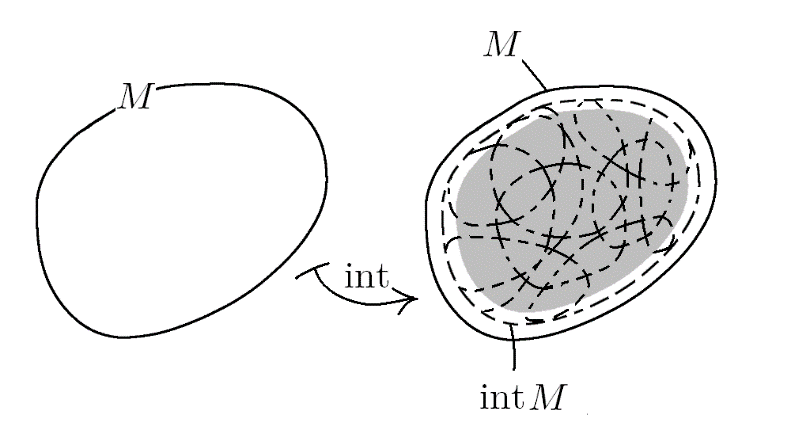
\includegraphics[width=93mm]{8.1.1.a.png}
\end{center}
\begin{thm}\label{8.1.1.2}
位相空間$\left( S,\mathfrak{O} \right)$において、$\forall M \in \mathfrak{P}(S)$に対し、その集合$M$の開核${\mathrm{int}}M$が集合$S'$であるならそのときに限り、次のこといずれも成り立つ、
\begin{itemize}
\item
  $S' \subseteq M$が成り立つ。
\item
  $S'\in \mathfrak{O}$が成り立つ。
\item
  $O \subseteq M$かつ$O \in \mathfrak{O}$が成り立つなら、$O \subseteq S'$が成り立つ。
\end{itemize}
さらに、順序集合$\left( \mathfrak{P}(S), \subseteq \right)$が与えられたとき、次式が成り立つ。
\begin{align*}
{\mathrm{int}}M = \max\left\{ O \in \mathfrak{O} \middle| O \subseteq M \right\}
\end{align*}
\end{thm}
\begin{proof}
位相空間$\left( S,\mathfrak{O} \right)$において、その集合$S$の任意の部分集合$M$の開核${\mathrm{int}}M$が集合$S'$であるなら、その集合$S'$はその集合$S$の部分集合で和集合$\bigcup_{\scriptsize \begin{matrix}
O \in \mathfrak{O} \\
O \subseteq M \\
\end{matrix}} O$に等しい。ここで、$O \subseteq M$が成り立つので、$\bigcup_{\scriptsize \begin{matrix}
O \in \mathfrak{O} \\
O \subseteq M \\
\end{matrix}} O \subseteq M$が成り立つかつ、$O \in \mathfrak{O}$と位相の定義より$\bigcup_{\scriptsize \begin{matrix}
O \in \mathfrak{O} \\
O \subseteq M \\
\end{matrix}} O\in \mathfrak{O}$が成り立つかつ、$O \subseteq M$なる任意のその位相$\mathfrak{O}$の元$O$に対し、$O \subseteq \bigcup_{\scriptsize \begin{matrix}
O \in \mathfrak{O} \\
O \subseteq M \\
\end{matrix}} O$が成り立つので、全称除去より$O \subseteq M \land O \in \mathfrak{O \Rightarrow}O \subseteq \bigcup_{\scriptsize \begin{matrix}
O \in \mathfrak{O} \\
O \subseteq M \\
\end{matrix}} O$が成り立つ。したがって、その集合$M$の開核${\mathrm{int}}M$が集合$S'$であるならそのときに限り、次のこといずれも成り立つ。
\begin{itemize}
\item
  $S' \subseteq M$が成り立つ。
\item
  $S'\in \mathfrak{O}$が成り立つ。
\item
  $O \subseteq M$かつ$O \in \mathfrak{O}$が成り立つなら、$O \subseteq S'$が成り立つ。
\end{itemize}\par
逆に、これらが成り立つなら、その和集合$\bigcup_{\scriptsize \begin{matrix}
O \in \mathfrak{O} \\
O \subseteq M \\
\end{matrix}} O$は上記の議論によりこれらを満たすので、その集合$S'$はその和集合$\bigcup_{\scriptsize \begin{matrix}
O \in \mathfrak{O} \\
O \subseteq M \\
\end{matrix}} O$とおくことができる。ここで、これらを満たすその和集合$\bigcup_{\scriptsize \begin{matrix}
O \in \mathfrak{O} \\
O \subseteq M \\
\end{matrix}} O$ではない集合$S''$が存在すると仮定すると、$S'' \subseteq M$かつ$S''\in \mathfrak{O}$が成り立つので、$S'' \subseteq \bigcup_{\scriptsize \begin{matrix}
O \in \mathfrak{O} \\
O \subseteq M \\
\end{matrix}} O$が成り立つが、これは$\bigcup_{\scriptsize \begin{matrix}
O \in \mathfrak{O} \\
O \subseteq M \\
\end{matrix}} O \subseteq M$かつ$\bigcup_{\scriptsize \begin{matrix}
O \in \mathfrak{O} \\
O \subseteq M \\
\end{matrix}} O\in \mathfrak{O}$が成り立つなら、$\bigcup_{\scriptsize \begin{matrix}
O \in \mathfrak{O} \\
O \subseteq M \\
\end{matrix}} O \subseteq S''$が成り立つことに矛盾する。したがって、その集合$S'$はその和集合$\bigcup_{\scriptsize \begin{matrix}
O \in \mathfrak{O} \\
O \subseteq M \\
\end{matrix}} O$である必要がありその集合$M$の開核${\mathrm{int}}M$が集合$S'$である。\par
さらに、順序集合$\left( \mathfrak{P}(S), \subseteq \right)$が与えられたとき、次のことが成り立つなら、
\begin{itemize}
\item
  ${\mathrm{int}}M \subseteq M$が成り立つ。
\item
  ${\mathrm{int}}M\in \mathfrak{O}$が成り立つ。
\item
  $O \subseteq M$かつ$O \in \mathfrak{O}$が成り立つなら、$O \subseteq {\mathrm{int}}M$が成り立つ。
\end{itemize}
これは次のように書き換えられることができる。
\begin{align*}
\forall O \in \left\{ O \in \mathfrak{O} \middle| O \subseteq M \right\}\left[ O \subseteq {\mathrm{int}}M \right]
\end{align*}
したがって、最大元の定義より次式が成り立つ。
\begin{align*}
{\mathrm{int}}M = \max\left\{ O \in \mathfrak{O} \middle| O \subseteq M \right\}
\end{align*}
\end{proof}
\begin{thm}\label{8.1.1.3}
位相空間$\left( S,\mathfrak{O} \right)$の開核について、次のことが成り立つ。
\begin{itemize}
\item
  $\forall M \in \mathfrak{P}(S)$に対し、$M \in \mathfrak{O}$が成り立つならそのときに限り、${\mathrm{int}}M = M$が成り立つ。
\item
  $\forall M,N \in \mathfrak{P}(S)$に対し、$M \subseteq N$が成り立つなら、${\mathrm{int}}M \subseteq {\mathrm{int}}N$が成り立つ。
\end{itemize}
\end{thm}
\begin{proof}
位相空間$\left( S,\mathfrak{O} \right)$が与えられたとき、$\forall M \in \mathfrak{P}(S)$に対し、$M \in \mathfrak{O}$が成り立つなら、$M \subseteq M$が成り立つかつ、$M \in \mathfrak{O}$が成り立つかつ、$O \subseteq M$かつ$O \in \mathfrak{O}$が成り立つなら、$O \subseteq M$が成り立つので、${\mathrm{int}}M = M$が成り立つ。逆に、${\mathrm{int}}M = M$が成り立つなら、$M \in \mathfrak{O}$が成り立つ。\par
$\forall M,N \in \mathfrak{P}(S)$に対し、$M \subseteq N$が成り立つときを考える。開核${\mathrm{int}}M$について、${\mathrm{int}}M \subseteq M$が成り立つかつ、${\mathrm{int}}M\in \mathfrak{O}$が成り立つかつ、$O \subseteq M$かつ$O \in \mathfrak{O}$が成り立つなら、$O \subseteq {\mathrm{int}}M$が成り立つ。開核${\mathrm{int}}N$についても同様である。以上より、${\mathrm{int}}M \subseteq M \subseteq N$が成り立つかつ、${\mathrm{int}}M\in \mathfrak{O}$が成り立つので、${\mathrm{int}}M \subseteq {\mathrm{int}}N$が成り立つ。
\end{proof}
%\hypertarget{ux9589ux96c6ux5408}{%
\subsubsection{閉集合}%\label{ux9589ux96c6ux5408}}
\begin{dfn}
位相空間$(S,\mathfrak{O})$において開集合のその集合$S$に対する補集合となるその集合$S$の部分集合をこの位相空間$\left( S,\mathfrak{O} \right)$の閉集合という。即ち、$S \setminus A \in \mathfrak{O}$なる集合$A$がその位相空間$\left( S,\mathfrak{O} \right)$の閉集合である。位相空間$(S,\ \mathfrak{O})$の閉集合全体の集合$\left\{ A \in \mathfrak{P}(S) \middle| S \setminus A \in \mathfrak{O} \right\}$をその位相空間$(S,\mathfrak{O})$の閉集合系という。
\end{dfn}
\begin{thm}\label{8.1.1.4}
位相空間$\left( S,\mathfrak{O} \right)$において、次のことが成り立つ。
\begin{itemize}
\item
  $S,\emptyset \in \mathfrak{A}$が成り立つ。
\item
  $\forall A,B \in \mathfrak{A}$に対し、$A \cup B \in \mathfrak{A}$が成り立つ。
\item
  任意の添数集合$\varLambda$によって添数づけられたその集合$\mathfrak{A}$の元の族$\left\{ A_{\lambda} \right\}_{\lambda \in \varLambda}$において$\bigcap_{\lambda \in \varLambda} A_{\lambda}\in \mathfrak{A}$が成り立つ。
\end{itemize}
\end{thm}
\begin{proof}
位相空間$(S,\mathfrak{O})$において、その位相空間$(S,\mathfrak{O})$の閉集合系を$\mathfrak{A}$と添数集合$\varLambda$によって添数づけられたそれらの集合$\mathfrak{O}$の元の族を$\left\{ O_{\lambda} \right\}_{\lambda \in \varLambda}$とし$A_{\lambda} = S \setminus O_{\lambda}$とおくと、添数集合$\varLambda$によって添数づけられたそれらの集合$\mathfrak{A}$の元の族$\left\{ A_{\lambda} \right\}_{\lambda \in \varLambda}$が得られる。したがって、次のようになる。
\begin{align*}
S,\emptyset \in \mathfrak{O \Leftrightarrow}S \setminus S,S \setminus \emptyset \in \mathfrak{O \Leftrightarrow}S,\emptyset \in \mathfrak{A}
\end{align*}
$\forall A,B \in \mathfrak{A}$に対し、次のようになる。
\begin{align*}
A,B \in \mathfrak{A} &\Leftrightarrow S \setminus A,S \setminus B \in \mathfrak{O}\\
&\Rightarrow S \setminus A \cap S \setminus B \in \mathfrak{O}\\
&\Leftrightarrow S \setminus (A \cup B)\in \mathfrak{O}\\
&\Leftrightarrow A \cup B \in \mathfrak{A}
\end{align*}
任意の添数集合$\varLambda$に対し、次のようになる。
\begin{align*}
\bigcup_{\lambda \in \varLambda} O_{\lambda}\in \mathfrak{O} &\Leftrightarrow S \setminus \bigcup_{\lambda \in \varLambda} O_{\lambda}\in \mathfrak{A}\\
&\Leftrightarrow \bigcap_{\lambda \in \varLambda} \left( S \setminus O_{\lambda} \right)\in \mathfrak{A}\\
&\Leftrightarrow \bigcap_{\lambda \in \varLambda} A_{\lambda}\in \mathfrak{A}
\end{align*}
\end{proof}
\begin{thm}\label{8.1.1.5}
その集合$S$の部分集合系$\mathfrak{A}$で上の3つの条件たちが満たされれば、その集合$\mathfrak{A}$が位相空間$\left( S,\mathfrak{O} \right)$の閉集合系と一致できるその位相$\mathfrak{O}$がただ1つに決まる。しかも、その位相$\mathfrak{O}$は次式を満たす。
\begin{align*}
\mathfrak{O}=\left\{ S \setminus A \in \mathfrak{P}(S) \middle| A \in \mathfrak{A} \right\}
\end{align*}
\end{thm}
\begin{proof}
その集合$S$の部分集合系$\mathfrak{A}$が次の3つの条件たちを満たすとしよう。
\begin{itemize}
\item
  $S,\emptyset \in \mathfrak{A}$が成り立つ。
\item
  $\forall A,B \in \mathfrak{A}$に対し、$A \cup B \in \mathfrak{A}$が成り立つ。
\item
  任意の添数集合$\varLambda$によって添数づけられたその集合$\mathfrak{A}$の元の族$\left\{ A_{\lambda} \right\}_{\lambda \in \varLambda}$において$\bigcap_{\lambda \in \varLambda} A_{\lambda}\in \mathfrak{A}$が成り立つ。
\end{itemize}
集合$\left\{ S \setminus A \in \mathfrak{P}(S) \middle| A \in \mathfrak{A} \right\}$を$\mathfrak{O}$とおくと、$S,\emptyset \in \mathfrak{A}$が成り立つなら、次のようになる。
\begin{align*}
S,\emptyset \in \mathfrak{A} &\Leftrightarrow S \setminus S,S \setminus \emptyset \in \mathfrak{O}\\
&\Leftrightarrow S,\emptyset \in \mathfrak{O}
\end{align*}
$\forall S \setminus A,S \setminus B \in \mathfrak{O}$に対し、$A \cup B \in \mathfrak{A}$が成り立つので、次のようになる。
\begin{align*}
S \setminus A \cap S \setminus B = S \setminus (A \cup B)\in \mathfrak{O}
\end{align*}
任意の添数集合$\varLambda$によって添数づけられたその集合$\mathfrak{O}$の元の族$\left\{ S \setminus A_{\lambda} \right\}_{\lambda \in \varLambda}$において、$\bigcap_{\lambda \in \varLambda} A_{\lambda}\in \mathfrak{A}$が成り立つので、次のようになる。
\begin{align*}
\bigcup_{\scriptsize \begin{matrix}
\lambda \in \varLambda \\
\end{matrix}} \left( S \setminus A_{\lambda} \right) = S \setminus \bigcap_{\lambda \in \varLambda} A_{\lambda}\in \mathfrak{O}
\end{align*}
以上より、その集合$\mathfrak{O}$は位相になる。\par
逆に、その位相$\mathfrak{O}$が与えられたとき、$\forall O \in \mathfrak{O}$に対し、次のようになる。
\begin{align*}
O \in \mathfrak{O} &\Leftrightarrow O \in \mathfrak{P}(S) \land S \setminus O \in \mathfrak{A}\\
&\Leftrightarrow S \setminus (S \setminus O)\in \mathfrak{P}(S) \land S \setminus O \in \mathfrak{A}
\end{align*}
したがって、その位相$\mathfrak{O}$がその集合$\mathfrak{A}$がその位相空間$\left( S,\mathfrak{O} \right)$の閉集合系と一致できる1つの位相$\mathfrak{O}$となっている。
\end{proof}
%\hypertarget{ux9589ux5305}{%
\subsubsection{閉包}%\label{ux9589ux5305}}
\begin{dfn}
位相空間$\left( S,\mathfrak{O} \right)$が与えられたとき、その位相空間$\left( S,\mathfrak{O} \right)$の閉集合系$\mathfrak{A}$を用いて$A \in \mathfrak{A}$かつ$M \subseteq A$なる集合$A$全体の積集合$\bigcap_{\scriptsize \begin{matrix}
A \in \mathfrak{A} \\
M \subseteq A \\
\end{matrix}} A$において、上記の閉集合についての定理より$\bigcap_{\scriptsize \begin{matrix}
A \in \mathfrak{A} \\
M \subseteq A \\
\end{matrix}} A\in \mathfrak{A}$が成り立つかつ、$\forall A \in \mathfrak{A}$に対し、$M \subseteq A$が成り立つなら、$\bigcap_{\scriptsize \begin{matrix}
A \in \mathfrak{A} \\
M \subseteq A \\
\end{matrix}} A \subseteq A$が成り立つ、即ち、その集合$\bigcap_{\scriptsize \begin{matrix}
A \in \mathfrak{A} \\
M \subseteq A \\
\end{matrix}} A$の大きさはいかなる、$M \subseteq A$が成り立つかつ、その閉集合系$\mathfrak{A}$に属するような集合$A$の大きさ以下になる。これは後述する定理\ref{8.1.1.6}で改めて述べられるが、このような集合$\bigcap_{\scriptsize \begin{matrix}
A \in \mathfrak{A} \\
M \subseteq A \\
\end{matrix}} A$をその集合$M$の閉包、触集合といい${\mathrm{cl}}M$、$Cl(M)$、$\overline{M}$、$M^{a}$などと書く、即ち、次式のように定義される。この閉包${\mathrm{cl}}M$の元を触点という。もちろん、その集合$M$の任意の元はその閉包${\mathrm{cl}}M$の触点である。
\begin{align*}
{\mathrm{cl}}M = \bigcap_{\scriptsize \begin{matrix}
A \in \mathfrak{A} \\
M \subseteq A \\
\end{matrix}} A
\end{align*}
\end{dfn}\par
これは次の図のように考えると、分かりやすかろう。
\begin{center}
  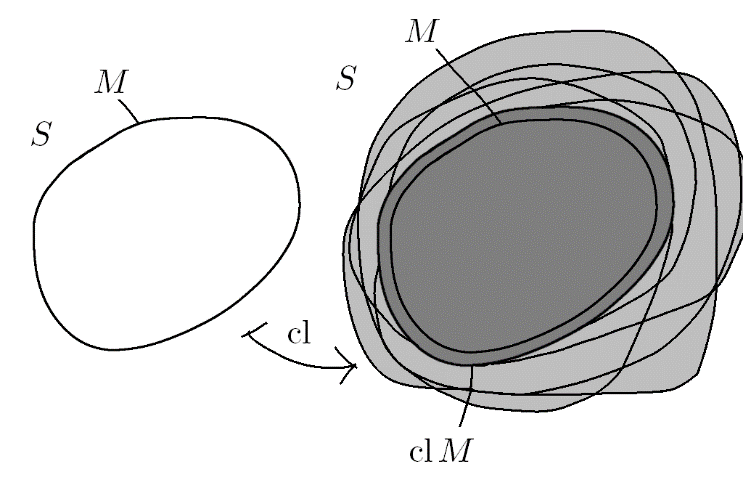
\includegraphics[width=86mm]{8.1.1.b.png}
\end{center}
\begin{thm}\label{8.1.1.6}
位相空間$\left( S,\mathfrak{O} \right)$において、$\forall M \in \mathfrak{P}(S)$に対し、その集合$M$の閉包${\mathrm{cl}}M$が集合$S'$であるならそのときに限り、次のこといずれも成り立つ。
\begin{itemize}
\item
  $M \subseteq S'$が成り立つ。
\item
  $S'\in \mathfrak{A}$が成り立つ。
\item
  $M \subseteq A$かつ$A \in \mathfrak{A}$が成り立つなら、$S' \subseteq A$が成り立つ。
\end{itemize}
さらに、順序集合$\left( \mathfrak{P}(S), \subseteq \right)$が与えられたとき、次式が成り立つ。
\begin{align*}
{\mathrm{cl}}M = \min\left\{ A \in \mathfrak{A} \middle| M \subseteq A \right\}
\end{align*}
\end{thm}
\begin{proof}
位相空間$\left( S,\mathfrak{O} \right)$において、その位相空間$\left( S,\mathfrak{O} \right)$の閉集合系$\mathfrak{A}$を用いてその集合$S$の任意の部分集合$M$の閉包${\mathrm{cl}}M$が集合$S'$であるなら、その集合$S'$はその集合$S$の部分集合で積集合$\bigcap_{\scriptsize \begin{matrix}
A \in \mathfrak{A} \\
M \subseteq A \\
\end{matrix}} A$に等しい。ここで、$M \subseteq A$が成り立つので、$M \subseteq \bigcap_{\scriptsize \begin{matrix}
A \in \mathfrak{A} \\
M \subseteq A \\
\end{matrix}} A$が成り立つかつ、$A \in \mathfrak{A}$と閉集合についての定理より$\bigcap_{\scriptsize \begin{matrix}
A \in \mathfrak{A} \\
M \subseteq A \\
\end{matrix}} A\in \mathfrak{A}$が成り立つかつ、$M \subseteq A$なる任意のその閉集合系$\mathfrak{A}$の元$A$に対し、$\bigcap_{\scriptsize \begin{matrix}
A \in \mathfrak{A} \\
M \subseteq A \\
\end{matrix}} A \subseteq A$が成り立つので、全称除去より$M \subseteq A \land A \in \mathfrak{A \Rightarrow}\bigcap_{\scriptsize \begin{matrix}
A \in \mathfrak{A} \\
M \subseteq A \\
\end{matrix}} A \subseteq A$が成り立つ。したがって、その集合$M$の閉包${\mathrm{cl}}M$が集合$S'$であるならそのときに限り、次のこといずれも成り立つ。
\begin{itemize}
\item
  $M \subseteq S'$が成り立つ。
\item
  $S'\in \mathfrak{A}$が成り立つ。
\item
  $M \subseteq A$かつ$A \in \mathfrak{A}$が成り立つなら、$S' \subseteq A$が成り立つ。
\end{itemize}\par
逆に、これらが成り立つなら、その積集合$\bigcap_{\scriptsize \begin{matrix}
A \in \mathfrak{A} \\
M \subseteq A \\
\end{matrix}} A$は上記の議論によりこれらを満たすので、その集合$S'$はその積集合$\bigcap_{\scriptsize \begin{matrix}
A \in \mathfrak{A} \\
M \subseteq A \\
\end{matrix}} A$とおくことができる。ここで、これらを満たすその積集合$\bigcap_{\scriptsize \begin{matrix}
A \in \mathfrak{A} \\
M \subseteq A \\
\end{matrix}} A$ではない集合$S''$が存在すると仮定すると、$M \subseteq S''$かつ$S''\in \mathfrak{A}$が成り立つので、$\bigcap_{\scriptsize \begin{matrix}
A \in \mathfrak{A} \\
M \subseteq A \\
\end{matrix}} A \subseteq S''$が成り立つが、これは$M \subseteq \bigcap_{\scriptsize \begin{matrix}
A \in \mathfrak{A} \\
M \subseteq A \\
\end{matrix}} A$かつ$\bigcap_{\scriptsize \begin{matrix}
A \in \mathfrak{A} \\
M \subseteq A \\
\end{matrix}} A\in \mathfrak{A}$が成り立つなら、$S'' \subseteq \bigcap_{\scriptsize \begin{matrix}
A \in \mathfrak{A} \\
M \subseteq A \\
\end{matrix}} A$が成り立つことに矛盾する。したがって、その集合$S'$はその積集合$\bigcap_{\scriptsize \begin{matrix}
A \in \mathfrak{A} \\
M \subseteq A \\
\end{matrix}} A$である必要がありその集合$M$の閉包${\mathrm{cl}}M$が集合$S'$である。\par
さらに、順序集合$\left( \mathfrak{P}(S), \subseteq \right)$が与えられたとき、次のことが成り立つなら、
\begin{itemize}
\item
  $M \subseteq {\mathrm{cl}}M$が成り立つ。
\item
  ${\mathrm{cl}}M\in \mathfrak{A}$が成り立つ。
\item
  $M \subseteq A$かつ$A \in \mathfrak{A}$が成り立つなら、${\mathrm{cl}}M \subseteq A$が成り立つ。
\end{itemize}
これは次のように書き換えられることができる。
\begin{align*}
\forall A \in \left\{ A \in \mathfrak{A} \middle| M \subseteq A \right\}\left[ {\mathrm{cl}}M \subseteq A \right]
\end{align*}
したがって、最小元の定義より次式が成り立つ。
\begin{align*}
{\mathrm{cl}}M = \min\left\{ A \in \mathfrak{A} \middle| M \subseteq A \right\}
\end{align*}
\end{proof}
\begin{thm}\label{8.1.1.7}
位相空間$\left( S,\mathfrak{O} \right)$の閉包について次のことが成り立つ。
\begin{itemize}
\item
  $\forall M \in \mathfrak{P}(S)$に対し、$M \in \mathfrak{A}$が成り立つならそのときに限り、${\mathrm{cl}}M = M$が成り立つ。
\item
  $\forall M,N \in \mathfrak{P}(S)$に対し、$M \subseteq N$が成り立つなら、${\mathrm{cl}}M \subseteq {\mathrm{cl}}N$が成り立つ。
\end{itemize}
\end{thm}
\begin{proof}
位相空間$\left( S,\mathfrak{O} \right)$が与えられたとき、その位相空間$\left( S,\mathfrak{O} \right)$の閉集合系$\mathfrak{A}$を用いて$\forall M \in \mathfrak{P}(S)$に対し、$M \in \mathfrak{A}$が成り立つなら、$M \subseteq M$が成り立つかつ、$M \in \mathfrak{A}$が成り立つかつ、$M \subseteq A$かつ$A \in \mathfrak{A}$が成り立つなら、$M \subseteq A$が成り立つので、${\mathrm{cl}}M = M$が成り立つ。逆に、${\mathrm{cl}}M = M$が成り立つなら、$M \in \mathfrak{A}$が成り立つ。\par
$\forall M,N \in \mathfrak{P}(S)$に対し、$M \subseteq N$が成り立つときを考える。閉包${\mathrm{cl}}M$について、${\mathrm{cl}}M \supseteq M$が成り立つかつ、${\mathrm{cl}}M\in \mathfrak{A}$が成り立つかつ、$M \subseteq A$かつ$A \in \mathfrak{A}$が成り立つなら、${\mathrm{cl}}M \subseteq A$が成り立つ。閉包${\mathrm{cl}}N$についても同様である。以上より、$M \subseteq N \subseteq {\mathrm{cl}}N$が成り立つかつ、${\mathrm{cl}}N\in \mathfrak{A}$が成り立つので、${\mathrm{cl}}M \subseteq {\mathrm{cl}}N$が成り立つ。
\end{proof}
%\hypertarget{ux958bux6838ux3068ux9589ux5305ux3068ux306eux95a2ux4fc2}{%
\subsubsection{開核と閉包との関係}%\label{ux958bux6838ux3068ux9589ux5305ux3068ux306eux95a2ux4fc2}}
\begin{thm}\label{8.1.1.8}
位相空間$\left( S,\mathfrak{O} \right)$と$M \in \mathfrak{P}(S)$なる集合$M$において、次式たちが成り立つ。このことをここでは開核と閉包との関係と呼ぶことにする\footnote{別の表記を用いれば、次のようになる。
\begin{align*}
  M^{ca} &= M^{ic}\\
  M^{cac} &= M^{i}\\
  M^{ci} &= M^{ac}\\
  M^{cic} &= M^{a}
\end{align*}}。
\begin{align*}
{\mathrm{cl}}(S \setminus M) &= S \setminus {\mathrm{int}}M\\
S \setminus {\mathrm{cl}}(S \setminus M) &= {\mathrm{int}}M\\
{\mathrm{int}}(S \setminus M) &= S \setminus {\mathrm{cl}}M\\
S \setminus {\mathrm{int}}(S \setminus M) &= {\mathrm{cl}}M
\end{align*}
\end{thm}\par
これは次の図のように考えると、分かりやすかろう。
\begin{center}
  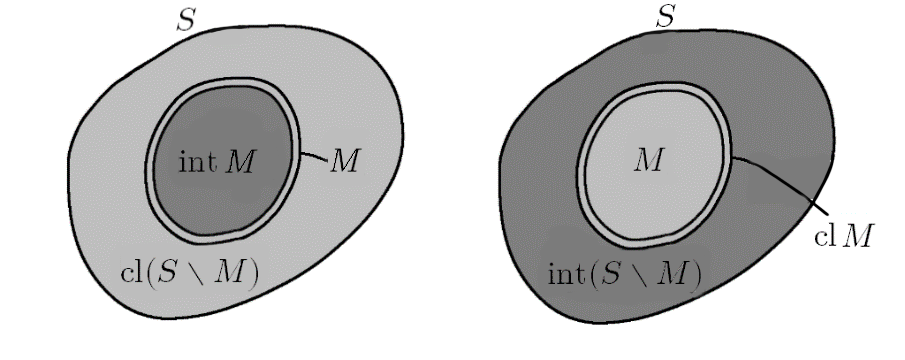
\includegraphics[width=104mm]{8.1.1.c.png}
\end{center}
ちなみに、1つの位相空間$\left( S,\mathfrak{O} \right)$において$S$対$\emptyset$、$\mathrm{int}$対$\mathrm{cl}$、$\cup$対$\cap$、$\subseteq$対$\supseteq$を交互に入れ替えたものも成り立つことが知られており、この性質を位相的双対律という。
\begin{proof}
位相空間$\left( S,\mathfrak{O} \right)$と$\forall M \in \mathfrak{P}(S)$なる集合$M$において、その位相空間$\left( S,\mathfrak{O} \right)$の閉集合系を$\mathfrak{A}$とおけば、$\forall A \in \mathfrak{A}$に対し${\mathrm{int}}M \subseteq M$より$S \setminus M \subseteq S \setminus {\mathrm{int}}M$が得られ、${\mathrm{int}}M = S \setminus S \setminus {\mathrm{int}}M\in \mathfrak{O}$と閉集合の定義より$S \setminus {\mathrm{int}}M\in \mathfrak{A}$が得られる。ここで、$S \setminus M \subseteq A$なる任意の閉集合$A$を考えると、$S \setminus A \subseteq S \setminus S \setminus M = M$と閉集合の定義より$S \setminus A \in \mathfrak{O}$かつ$S \setminus A \subseteq M$が得られる。ここで、その集合${\mathrm{int}}M$は$O \in \mathfrak{O}$かつ$O \subseteq M$なる開集合$O$全体の和集合$\bigcup_{\scriptsize \begin{matrix}
O \in \mathfrak{O} \\
O \subseteq M \\
\end{matrix}} O$でありその集合${\mathrm{int}}M$の大きさはいかなる、$O \subseteq M$が成り立つかつ、その位相$\mathfrak{O}$に属するような集合$O$の大きさ以上になるのであったので、$S \setminus A \subseteq {\mathrm{int}}M$が成り立つ。したがって、$S \setminus {\mathrm{int}}M\in \mathfrak{A}$かつ$S \setminus {\mathrm{int}}M \subseteq S \setminus S \setminus A = A$が得られる。ここで、その集合${\mathrm{cl}}(S \setminus M)$は$A \in \mathfrak{A}$かつ$S \setminus M \subseteq A$なる閉集合$A$全体の積集合$\bigcap_{\scriptsize \begin{matrix}
A \in \mathfrak{A} \\
M \subseteq A \\
\end{matrix}} A$でありその集合${\mathrm{cl}}(S \setminus M)$の大きさはいかなる、$M \subseteq A$が成り立つかつ、その閉集合系$\mathfrak{A}$に属するような集合$A$の大きさ以下になるのであったので、${\mathrm{cl}}(S \setminus M) = S \setminus {\mathrm{int}}M$が成り立つ。\par
これが用いられると、次のようになる。
\begin{align*}
S \setminus {\mathrm{cl}}(S \setminus M) &= S \setminus S \setminus {\mathrm{int}}M\\
&= {\mathrm{int}}M\\
{\mathrm{int}}(S \setminus M) &= S \setminus S \setminus {\mathrm{int}}(S \setminus M)\\
&= S \setminus {\mathrm{cl}}(S \setminus S \setminus M)\\
&= S \setminus {\mathrm{cl}}M\\
S \setminus {\mathrm{int}}(S \setminus M) &= {\mathrm{cl}}(S \setminus S \setminus M)\\
&= {\mathrm{cl}}M
\end{align*}
\end{proof}
\begin{thm}\label{8.1.1.9}
位相空間$\left( S,\mathfrak{O} \right)$が与えられたとする。$\forall a \in S$に対し、$a \in {\mathrm{cl}}M$が成り立つならそのときに限り、$\forall O \in \mathfrak{O}$に対し、$a \in O$が成り立つなら、$O \cap M \neq \emptyset$が成り立つ。
\end{thm}
\begin{proof}
位相空間$\left( S,\mathfrak{O} \right)$が与えられたとする。$\forall a \in S$に対し、$a \in {\mathrm{cl}}M$が成り立たないなら、$a \in S \setminus {\mathrm{cl}}M$が成り立つ。したがって、$a \in {\mathrm{int}}(S \setminus M)$が成り立つことになりその集合${\mathrm{int}}(S \setminus M)$はその位相$\mathfrak{O}$の開集合で${\mathrm{int}}(S \setminus M) \subseteq S \setminus M$が成り立つことから、次のようになるので、
\begin{align*}
{\mathrm{int}}(S \setminus M) \cap M \subseteq S \setminus M \cap M = \emptyset
\end{align*}
${\mathrm{int}}(S \setminus M) = \emptyset$が成り立つ。\par
逆に、$\exists O \in \mathfrak{O}$に対し、$O \cap M = \emptyset$が成り立つなら、$\forall a \in O$に対し、$a \in O$かつ$a \notin O \cap P$が成り立つことになり、したがって、$a \in O$かつ$a \notin M$が成り立つので、$O \subseteq S \setminus M$が成り立つ。ここで、その集合$O$が開集合で$O = {\mathrm{int}}O$が成り立つことに注意すれば、$O \subseteq {\mathrm{int}}(S \setminus M)$が成り立ち、${\mathrm{int}}(S \setminus M) = S \setminus {\mathrm{cl}}M$が成り立つので、その元$a$はその閉包${\mathrm{cl}}M$に属さない。\par
以上対偶律により、$\forall a \in S$に対し、$a \in {\mathrm{cl}}M$が成り立つならそのときに限り、$\forall O \in \mathfrak{O}$に対し、$a \in O$が成り立つなら、$O \cap M \neq \emptyset$が成り立つ。
\end{proof}
\begin{thm}\label{8.1.1.10}
位相空間$\left( S,\mathfrak{O} \right)$が与えられたとする。このとき、次のことが成り立つ。
\begin{itemize}
\item
  $\forall O \in \mathfrak{O\forall}M \in \mathfrak{P}(S)$に対し、$O \cap {\mathrm{cl}}M \subseteq {\mathrm{cl}}(O \cap M)$が成り立つ。
\item
  $\forall O \in \mathfrak{O\forall}M \in \mathfrak{P}(S)$に対し、$O \cap M = \emptyset$が成り立つなら、$O \cap {\mathrm{cl}}M = \emptyset$が成り立つ。
\end{itemize}
\end{thm}
\begin{proof} 位相空間$\left( S,\mathfrak{O} \right)$が与えられたとする。\par
$\forall O \in \mathfrak{O\forall}M \in \mathfrak{P}(S)\forall a \in O \cap {\mathrm{cl}}M$に対し、明らかに$a \in {\mathrm{cl}}M$が成り立ち、$a \in O'$なるその位相$\mathfrak{O}$の任意の開集合$O'$が与えられると、位相の定義よりその集合$O \cap O'$も開集合で$O \cap O' \cap M \neq \emptyset$が成り立つ。したがって、$a \in O'$なるその位相$\mathfrak{O}$の任意の開集合たち$O'$に対し、$O' \cap (O \cap M) \neq \emptyset$が成り立つので、$a \in {\mathrm{cl}}(O \cap M)$が成り立つ。以上より、$O \cap {\mathrm{cl}}M \subseteq {\mathrm{cl}}(O \cap M)$が成り立つ。\par
特に、$O \cap M = \emptyset$が成り立つなら、上記の議論により$O \cap {\mathrm{cl}}M \subseteq {\mathrm{cl}}\emptyset$が成り立つかつ、空集合$\emptyset$はその位相空間$\left( S,\mathfrak{O} \right)$での閉集合でもあるので、${\mathrm{cl}}\emptyset = \emptyset$が成り立つことになり、したがって、$O \cap {\mathrm{cl}}M = \emptyset$が成り立つ。
\end{proof}
%\hypertarget{ux958bux6838ux4f5cux7528ux5b50ux3068ux9589ux5305ux4f5cux7528ux5b50}{%
\subsubsection{開核作用子と閉包作用子}%\label{ux958bux6838ux4f5cux7528ux5b50ux3068ux9589ux5305ux4f5cux7528ux5b50}}
\begin{dfn}
位相空間$\left( S,\mathfrak{O} \right)$において、写像$int\mathfrak{:P}(S)\mathfrak{\rightarrow P}(S);M \mapsto int(M)$をその位相空間$\left( S,\mathfrak{O} \right)$における開核作用子という。
\end{dfn}
\begin{thm}\label{8.1.1.11}
位相空間$\left( S,\mathfrak{O} \right)$が与えられたとき、次のことが成り立つ。
\begin{itemize}
\item
  ${\mathrm{int}}S = S$が成り立つ。
\item
  $\forall M\in \mathfrak{P}(S)$に対し、${\mathrm{int}}M \subseteq M$が成り立つ。
\item
  $\forall M,N\in \mathfrak{P}(S)$に対し、${\mathrm{int}}(M \cap N) = {\mathrm{int}}M \cap {\mathrm{int}}N$が成り立つ。
\item
  $\forall M\in \mathfrak{P}(S)$に対し、${\mathrm{int}}{{\mathrm{int}}M} = {\mathrm{int}}M$が成り立つ。
\end{itemize}
\end{thm}\par
これは次の図のように考えると、分かりやすかろう。
\begin{center}
  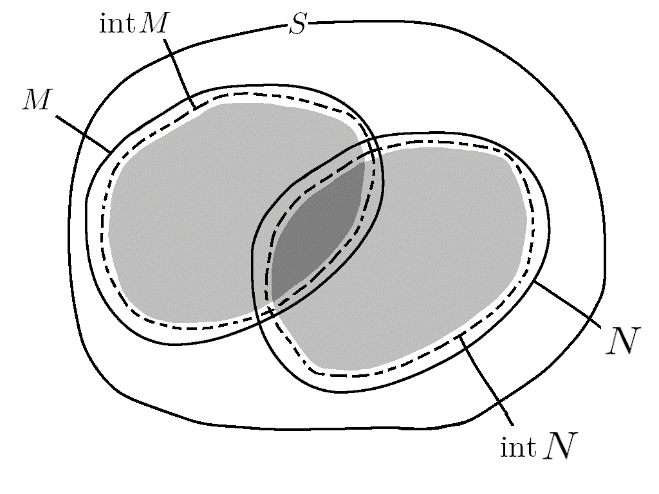
\includegraphics[width=80mm]{8.1.1.d.png}
\end{center}
\begin{proof} 位相空間$\left( S,\mathfrak{O} \right)$において、定理\ref{8.1.1.2}より$S \subseteq S$かつ$S \in \mathfrak{O}$かつ$O \subseteq S \land O \in \mathfrak{O} \Rightarrow O \subseteq S$が成り立つので、${\mathrm{int}}S = S$が得られる。\par
$\forall M \in \mathfrak{P}(S)$に対し、定義より明らかに${\mathrm{int}}M \subseteq M$が成り立つ。\par
これにより、$\forall M,N \in \mathfrak{P}(S)$に対し、${\mathrm{int}}M \cap {\mathrm{int}}N \subseteq M \cap N$が成り立つ。ここで、位相の定義と${\mathrm{int}}M,{\mathrm{int}}N\in \mathfrak{O}$より${\mathrm{int}}M \cap {\mathrm{int}}N\in \mathfrak{O}$が成り立つかつ、$O \subseteq M \cap N$なる任意の開集合$O$を考えると、$O \subseteq M$かつ$O \in \mathfrak{O}$が成り立つなら、$O \subseteq {\mathrm{int}}M$が成り立つことと$O \subseteq N$かつ$O \in \mathfrak{O}$が成り立つなら、$O \subseteq {\mathrm{int}}N$が成り立つことより$O \subseteq {\mathrm{int}}M \cap {\mathrm{int}}N$が得られる。したがって、定理\ref{8.1.1.2}より${\mathrm{int}}(M \cap N) = {\mathrm{int}}M \cap {\mathrm{int}}N$が成り立つ。\par
$\forall M\in \mathfrak{P}(S)$に対し、${\mathrm{int}}M \subseteq {\mathrm{int}}M$かつ${\mathrm{int}}M\in \mathfrak{O}$が成り立つかつ、$O \subseteq {\mathrm{int}}M$かつ$O \in \mathfrak{O}$が成り立つなら、$O \subseteq {\mathrm{int}}M$が成り立つことより${\mathrm{int}}{{\mathrm{int}}M} = {\mathrm{int}}M$が得られる。
\end{proof}
\begin{thm}\label{8.1.1.12}
空集合$\emptyset$でない集合$S$の各部分集合たちにその集合$S$の部分集合たちを対応させる写像$i:\mathfrak{P}(S)\mathfrak{\rightarrow P}(S)$で次のことが成り立つとする。
\begin{itemize}
\item
  $i(S) = S$が成り立つ。
\item
  $\forall M\in \mathfrak{P}(S)$に対し、$i(M) \subseteq M$が成り立つ。
\item
  $\forall M,N\in \mathfrak{P}(S)$に対し、$i(M \cap N) = i(M) \cap i(N)$が成り立つ。
\item
  $i \circ i = i$が成り立つ。
\end{itemize}
このとき、その写像$i$がその位相空間$\left( S,\mathfrak{O} \right)$における開核作用子と一致できる1つの位相$\mathfrak{O}$がただ1つに決まり、次式のように与えられる。
\begin{align*}
\mathfrak{O}=\left\{ M \in \mathfrak{P}(S) \middle| i(M) = M \right\}
\end{align*}
\end{thm}
\begin{proof}
空集合$\emptyset$でない集合$S$の各部分集合たちにその集合$S$の部分集合たちを対応させる写像$i:\mathfrak{P}(S)\mathfrak{\rightarrow P}(S)$で次のことが成り立つとする。
\begin{itemize}
\item
  $i(S) = S$が成り立つ。
\item
  $\forall M\in \mathfrak{P}(S)$に対し、$i(M) \subseteq M$が成り立つ。
\item
  $\forall M,N\in \mathfrak{P}(S)$に対し、$i(M \cap N) = i(M) \cap i(N)$が成り立つ。
\item
  $i \circ i = i$が成り立つ。
\end{itemize}
ここで、$\mathfrak{O}=\left\{ M \in \mathfrak{P}(S) \middle| i(M) = M \right\}$なる集合$\mathfrak{O}$が位相空間$\left( S,\mathfrak{O} \right)$における位相に一致しその写像$i$がその位相空間$\left( S,\mathfrak{O} \right)$の開核作用子と一致することを示そう。\par
仮定と空集合はどの集合にも含まれることより次のようになる。
\begin{align*}
i(S) = S \land i(\emptyset) \subseteq \emptyset \land \emptyset \subseteq i(\emptyset) &\Leftrightarrow i(S) = S \land i(\emptyset) = \emptyset\\
&\Leftrightarrow S,\emptyset \in \mathfrak{O}
\end{align*}
$\forall O,P \in \mathfrak{O}$に対し、仮定とこれの数学的帰納法より次のようになる。
\begin{align*}
O,P \in \mathfrak{O} &\Leftrightarrow i(O) = O \land i(P) = P\\
&\Rightarrow i(O \cap P) = i(O) \cap i(P) = O \cap P\\
&\Leftrightarrow O \cap P \in \mathfrak{O}
\end{align*}
任意の添数集合$\varLambda$によって添数づけられたその集合$\mathfrak{O}$の元の族$\left\{ O_{\lambda} \right\}_{\lambda \in \varLambda}$が与えられると、$\forall\lambda \in \varLambda$に対し、仮定より次のようになる。
\begin{align*}
O_{\lambda}\in \mathfrak{O} &\Leftrightarrow O_{\lambda}\in \mathfrak{O \land}O_{\lambda} \subseteq \bigcup_{\lambda \in \varLambda} O_{\lambda} \land i\left( \bigcup_{\lambda \in \varLambda} O_{\lambda} \right) \subseteq \bigcup_{\lambda \in \varLambda} O_{\lambda}\\
&\Leftrightarrow i\left( O_{\lambda} \right) = O_{\lambda} \land O_{\lambda} \subseteq \bigcup_{\lambda \in \varLambda} O_{\lambda} \land i\left( \bigcup_{\lambda \in \varLambda} O_{\lambda} \right) \subseteq \bigcup_{\lambda \in \varLambda} O_{\lambda}\\
&\Leftrightarrow i\left( O_{\lambda} \right) = O_{\lambda} \subseteq i\left( \bigcup_{\lambda \in \varLambda} O_{\lambda} \right) \land i\left( \bigcup_{\lambda \in \varLambda} O_{\lambda} \right) \subseteq \bigcup_{\lambda \in \varLambda} O_{\lambda}\\
&\Rightarrow \bigcup_{\lambda \in \varLambda} O_{\lambda} \subseteq i\left( \bigcup_{\lambda \in \varLambda} O_{\lambda} \right) \land i\left( \bigcup_{\lambda \in \varLambda} O_{\lambda} \right) \subseteq \bigcup_{\lambda \in \varLambda} O_{\lambda}\\
&\Leftrightarrow i\left( \bigcup_{\lambda \in \varLambda} O_{\lambda} \right) = \bigcup_{\lambda \in \varLambda} O_{\lambda}\\
&\Leftrightarrow \bigcup_{\lambda \in \varLambda} O_{\lambda}\in \mathfrak{O}
\end{align*}
以上より次の条件たちが満たされその集合$\mathfrak{O}$は位相に相当する。
\begin{itemize}
\item
  $S,\emptyset \in \mathfrak{O}$が成り立つ。
\item
  $\forall O,P \in \mathfrak{O}$に対し、$O \cap P \in \mathfrak{O}$が成り立つ。
\item
  任意の添数集合$\varLambda$によって添数づけられたその集合$\mathfrak{O}$の元の族$\left\{ O_{\lambda} \right\}_{\lambda \in \varLambda}$において$\bigcup_{\lambda \in \varLambda} O_{\lambda}\in \mathfrak{O}$が成り立つ。
\end{itemize}\par
また、次のようになることから、
\begin{itemize}
\item
  $i(M) \subseteq M$が成り立つ。
\item
  $i \circ i(M) = i\left( i(M) \right) = i(M)$より$i(M)\in \mathfrak{O}$が成り立つ。
\item
  $O \subseteq M$かつ$O \in \mathfrak{O}$が成り立つなら、$i(O) \subseteq i(M)$かつ$i(O) = O$が成り立つことにより、$O \subseteq i(M)$が成り立つ。
\end{itemize}
定理\ref{8.1.1.2}よりその集合$i(M)$はその集合$M$の開核である。
\end{proof}
\begin{thm}\label{8.1.1.13}
位相空間$\left( S,\mathfrak{O} \right)$において、写像$cl\mathfrak{:P}(S)\mathfrak{\rightarrow P}(S);M \mapsto {\mathrm{cl}}M$をその位相空間$\left( S,\mathfrak{O} \right)$における閉包作用子という。これについて次式たちが成り立つ。
\begin{itemize}
\item
  ${\mathrm{cl}}\emptyset = \emptyset$が成り立つ。
\item
  $\forall M\in \mathfrak{P}(S)$に対し、$M \subseteq {\mathrm{cl}}M$が成り立つ。
\item
  $\forall M,N\in \mathfrak{P}(S)$に対し、${\mathrm{cl}}(M \cup N) = {\mathrm{cl}}M \cup {\mathrm{cl}}N$が成り立つ。
\item
  $\forall M\in \mathfrak{P}(S)$に対し、${\mathrm{cl}}{{\mathrm{cl}}M} = {\mathrm{cl}}M$が成り立つ。
\end{itemize}
\end{thm}\par
これは次の図のように考えると、分かりやすかろう。
\begin{center}
  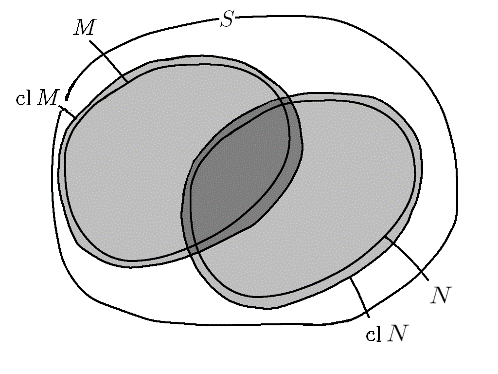
\includegraphics[width=80mm]{8.1.1.e.png}
\end{center}
\begin{proof}
位相空間$\left( S,\mathfrak{O} \right)$において、これの閉集合系$\mathfrak{A}$が与えられたとき、定理\ref{8.1.1.6}より$\emptyset \subseteq \emptyset$かつ$\mathfrak{\emptyset \in A}$かつ$\emptyset \subseteq A \land A \in \mathfrak{A} \Rightarrow \emptyset \subseteq A$が成り立つので、${\mathrm{cl}}\emptyset = \emptyset$が得られる。\par
$\forall M \in \mathfrak{P}(S)$に対し、定義より明らかに$M \subseteq {\mathrm{cl}}M$が成り立つ。\par
これにより、$\forall M,N \in \mathfrak{P}(S)$に対し、$M \cup N \subseteq {\mathrm{cl}}M \cup {\mathrm{cl}}N$が成り立つ。ここで、${\mathrm{cl}}M,{\mathrm{cl}}N\in \mathfrak{A}$より${\mathrm{cl}}M \cup {\mathrm{cl}}N\in \mathfrak{A}$かつ$M \cup N \subseteq A$なる任意の閉集合$A$を考えると、$M \subseteq A$かつ$A \in \mathfrak{A}$が成り立つなら、${\mathrm{cl}}M \subseteq A$が成り立つことと$N \subseteq A$かつ$A \in \mathfrak{A}$が成り立つなら、${\mathrm{cl}}N \subseteq A$が成り立つことより${\mathrm{int}}M \cup {\mathrm{int}}N \subseteq A$が得られる。したがって、定理\ref{8.1.1.6}より${\mathrm{cl}}(M \cup N) = {\mathrm{cl}}M \cup {\mathrm{cl}}N$が成り立つ。\par
$\forall M\in \mathfrak{P}(S)$に対し、${\mathrm{cl}}M \subseteq {\mathrm{cl}}M$かつ${\mathrm{cl}}M\in \mathfrak{A}$が成り立つかつ、${\mathrm{cl}}M \subseteq A$かつ$A \in \mathfrak{A}$が成り立つなら、${\mathrm{cl}}M \subseteq A$が成り立つことより${\mathrm{cl}}{{\mathrm{cl}}M} = {\mathrm{cl}}M$が得られる。
\end{proof}
\begin{thm}\label{8.1.1.14}
空集合$\emptyset$でない集合$S$の各部分集合たちにその集合$S$の部分集合たちを対応させる写像$a:\mathfrak{P}(S)\mathfrak{\rightarrow P}(S)$で次のことが成り立つとする。
\begin{itemize}
\item
  $a(\emptyset) = \emptyset$が成り立つ。
\item
  $\forall M \in \mathfrak{P}(S)$に対し、$M \subseteq a(M)$が成り立つ。
\item
  $\forall M,N \in \mathfrak{P}(S)$に対し、$a(M \cup N) = a(M) \cup a(N)$が成り立つ。
\item
  $a \circ a = a$が成り立つ。
\end{itemize}
このとき、その写像$aがその位相空間\left( S,\mathfrak{O} \right)$における閉包作用子と一致できる1つの位相$\mathfrak{O}$がただ1つに決まり、次式のように与えられる。
\begin{align*}
\mathfrak{O}=\left\{ S \setminus M \in \mathfrak{P}(S) \middle| a(M) = M \right\}
\end{align*}
\end{thm}\par
これを位相$\mathfrak{O}$の公理系とする場合があり、このときの公理系をKuratowskiの公理系という。
\begin{proof}
空集合$\emptyset$でない集合$S$の各部分集合たちにその集合$S$の部分集合たちを対応させる写像$a:\mathfrak{P}(S)\mathfrak{\rightarrow P}(S)$で次のことが成り立つとする。
\begin{itemize}
\item
  $a(\emptyset) = \emptyset$が成り立つ。
\item
  $\forall M \in \mathfrak{P}(S)$に対し、$M \subseteq a(M)$が成り立つ。
\item
  $\forall M,N \in \mathfrak{P}(S)$に対し、$a(M \cup N) = a(M) \cup a(N)$が成り立つ。
\item
  $a \circ a = a$が成り立つ。
\end{itemize}\par
ここで、$\mathfrak{O}=\left\{ S \setminus M \in \mathfrak{P}(S) \middle| a(M) = M \right\}$なる集合$\mathfrak{O}$が位相空間$\left( S,\mathfrak{O} \right)$における位相に、$\mathfrak{A} =\left\{ M \in \mathfrak{P}(S) \middle| a(M) = M \right\}$、即ち、$\mathfrak{A }=\left\{ M \in \mathfrak{P}(S) \middle| S \setminus M \in \mathfrak{O} \right\}$なる集合$\mathfrak{A}$がその位相空間$\left( S,\mathfrak{O} \right)$における閉集合系に一致しその写像$a$がその位相空間$\left( S,\mathfrak{O} \right)$の閉包作用子と一致することを示そう。\par
仮定とその集合$S$はその位相空間$\left( S,\mathfrak{O} \right)$でのどの集合にも含まれることより次のようになる。
\begin{align*}
a(\emptyset) = \emptyset \land S \subseteq a(S) \land a(S) \subseteq S &\Leftrightarrow a(S) = S \land a(\emptyset) = \emptyset\\
&\Leftrightarrow S,\emptyset \in \mathfrak{A}\\
&\Leftrightarrow S \setminus S,S \setminus \emptyset \in \mathfrak{O}\\
&\Leftrightarrow S,\emptyset \in \mathfrak{O}
\end{align*}
$\forall O,P \in \mathfrak{O}$に対し、仮定とこれの数学的帰納法より次のようになる。
\begin{align*}
O,P \in \mathfrak{O} &\Leftrightarrow a(S \setminus O) = S \setminus O \land a(S \setminus P) = S \setminus P\\
&\Rightarrow a(S \setminus O \cup S \setminus P) = a(S \setminus O) \cup a\left( S\setminus P \right) = S \setminus O \cup S \setminus P\\
&\Leftrightarrow S \setminus O \cup S \setminus P = S \setminus (O \cap P)\in \mathfrak{A}\\
&\Leftrightarrow O \cap P \in \mathfrak{O}
\end{align*}\par
任意の添数集合$\varLambda$によって添数づけられたその集合$\mathfrak{O}$の元の族$\left\{ O_{\lambda} \right\}_{\lambda \in \varLambda}$が与えられると、$\forall\lambda \in \varLambda$に対し、仮定より次のようになる。
\begin{align*}
O_{\lambda}\in \mathfrak{O} &\Leftrightarrow O_{\lambda}\in \mathfrak{O \land}O_{\lambda} \subseteq \bigcup_{\lambda \in \varLambda} O_{\lambda} \land S \setminus \bigcup_{\lambda \in \varLambda} O_{\lambda} \subseteq a\left( S \setminus \bigcup_{\lambda \in \varLambda} O_{\lambda} \right)\\
&\Leftrightarrow a\left( S \setminus O_{\lambda} \right) = S \setminus O_{\lambda} \land S \setminus \bigcup_{\lambda \in \varLambda} O_{\lambda} \subseteq S \setminus O_{\lambda} \land S \setminus \bigcup_{\lambda \in \varLambda} O_{\lambda} \subseteq a\left( S \setminus \bigcup_{\lambda \in \varLambda} O_{\lambda} \right)\\
&\Leftrightarrow a\left( S \setminus O_{\lambda} \right) = S \setminus O_{\lambda} \land S \setminus \bigcup_{\lambda \in \varLambda} O_{\lambda} \subseteq S \setminus O_{\lambda} \land S \setminus \bigcup_{\lambda \in \varLambda} O_{\lambda} \subseteq a\left( S \setminus \bigcup_{\lambda \in \varLambda} O_{\lambda} \right)\\
&\Rightarrow a\left( S \setminus O_{\lambda} \right) = S \setminus O_{\lambda} \land a\left( S \setminus \bigcup_{\lambda \in \varLambda} O_{\lambda} \right) \subseteq {\mathrm{cl}}\left( S \setminus O_{\lambda} \right) \land S \setminus \bigcup_{\lambda \in \varLambda} O_{\lambda} \subseteq a\left( S \setminus \bigcup_{\lambda \in \varLambda} O_{\lambda} \right)\\
&\Rightarrow a\left( S \setminus \bigcup_{\lambda \in \varLambda} O_{\lambda} \right) \subseteq S \setminus O_{\lambda} \land S \setminus \bigcup_{\lambda \in \varLambda} O_{\lambda} \subseteq a\left( S \setminus \bigcup_{\lambda \in \varLambda} O_{\lambda} \right)\\
&\Rightarrow a\left( S \setminus \bigcup_{\lambda \in \varLambda} O_{\lambda} \right) \subseteq \bigcap_{\lambda \in \varLambda} \left( S \setminus O_{\lambda} \right) \land S \setminus \bigcup_{\lambda \in \varLambda} O_{\lambda} \subseteq a\left( S \setminus \bigcup_{\lambda \in \varLambda} O_{\lambda} \right)\\
&\Leftrightarrow a\left( S \setminus \bigcup_{\lambda \in \varLambda} O_{\lambda} \right) \subseteq S \setminus \bigcup_{\lambda \in \varLambda} O_{\lambda} \land S \setminus \bigcup_{\lambda \in \varLambda} O_{\lambda} \subseteq a\left( S \setminus \bigcup_{\lambda \in \varLambda} O_{\lambda} \right)\\
&\Leftrightarrow a\left( S \setminus \bigcup_{\lambda \in \varLambda} O_{\lambda} \right) = S \setminus \bigcup_{\lambda \in \varLambda} O_{\lambda}\\
&\Leftrightarrow \bigcup_{\lambda \in \varLambda} O_{\lambda}\in \mathfrak{O}
\end{align*}\par
以上より次の条件たちが満たされその集合$\mathfrak{O}$は位相に相当する。
\begin{itemize}
\item
  $S,\emptyset \in \mathfrak{O}$が成り立つ。
\item
  $\forall O,P \in \mathfrak{O}$に対し、$O \cap P \in \mathfrak{O}$が成り立つ。
\item
  任意の添数集合$\varLambda$によって添数づけられたその集合$\mathfrak{O}$の元の族$\left\{ O_{\lambda} \right\}_{\lambda \in \varLambda}$において$\bigcup_{\lambda \in \varLambda} O_{\lambda}\in \mathfrak{O}$が成り立つ。
\end{itemize}\par
また、$\forall M \in \mathfrak{P}(S)$に対し、次のようになることから、
\begin{itemize}
\item
  $M \subseteq a(M)$が成り立つ。
\item
  $a \circ a(M) = a\left( a(M) \right) = a(M)$より$a(M)\in \mathfrak{A}$が成り立つ。
\item
  $M \subseteq A$かつ$A \in \mathfrak{A}$が成り立つなら、$a(M) \subseteq a(A) = A$が成り立つことにより、$a(M) \subseteq A$が成り立つ。
\end{itemize}
\ref{8.1.1.6}よりその集合$a(M)$はその集合$M$の閉包である。
\end{proof}
%\hypertarget{ux5916ux90e8ux3068ux5883ux754c}{%
\subsubsection{外部と境界}%\label{ux5916ux90e8ux3068ux5883ux754c}}
\begin{dfn}
位相空間$\left( S,\mathfrak{O} \right)$において、$M \in \mathfrak{P}(S)$なる集合$M$の補集合$S \setminus M$の開核${\mathrm{int}}(S \setminus M)$をその集合$M$の外部といい、${\mathrm{ext}}M$、$M^{e}$などと書く、即ち、次式のようになる。この外部$M^{e}$の元を外点という。
\begin{align*}
{\mathrm{ext}}M = {\mathrm{int}}(S \setminus M)
\end{align*}
\end{dfn}
これは次の図のように考えると、分かりやすかろう。
\begin{center}
  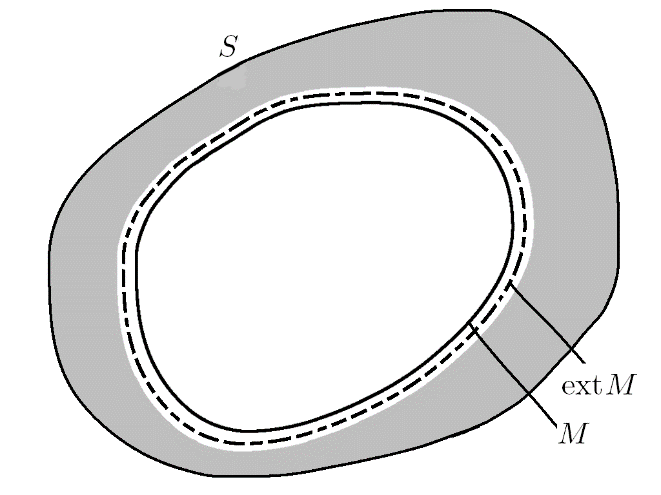
\includegraphics[width=76mm]{8.1.1.f.png}
\end{center}
\begin{thm}\label{8.1.1.15}
位相空間$\left( S,\mathfrak{O} \right)$において、$\forall M \in \mathfrak{P}(S)$に対し、次式が成り立つ\footnote{別の表記を用いれば、次のようになる。
\begin{align*}
  M^{e}&\in \mathfrak{O}\\
  M^{e} &= M^{ac}\\
  S &= M^{a} \sqcup M^{e}
  \end{align*}}。
\begin{align*}
{\mathrm{ext}}M&\in \mathfrak{O}\\
{\mathrm{ext}}M &= S \setminus {\mathrm{cl}}M\\
S &= {\mathrm{cl}}M \sqcup {\mathrm{ext}}M
\end{align*}
\end{thm}
\begin{proof}
これらは定義と開核と閉包との関係より明らかである。実際、位相空間$\left( S,\mathfrak{O} \right)$が与えられ$M \in \mathfrak{P}(S)$なる集合$M$において、開核は定義より位相$\mathfrak{O}$に属するので、${\mathrm{ext}}M = {\mathrm{int}}(S \setminus M)\in \mathfrak{O}$が成り立ち、開核と閉包との関係より${\mathrm{int}}(S \setminus M) = S \setminus {\mathrm{cl}}M$が成り立つので、${\mathrm{ext}}M = S \setminus {\mathrm{cl}}M$が成り立ち、これと差集合の性質より$S = {\mathrm{cl}}M \sqcup S \setminus {\mathrm{cl}}M = {\mathrm{cl}}M \sqcup {\mathrm{ext}}M$が成り立つ。
\end{proof}
\begin{dfn}
位相空間$\left( S,\mathfrak{O} \right)$において、$M \in \mathfrak{P}(S)$なる集合$M$の閉包${\mathrm{cl}}M$から開核${\mathrm{int}}M$への差集合${\mathrm{cl}}M \setminus {\mathrm{int}}M$をその集合$M$の境界といい、$\partial M$、$\partial(M)$、${bd}M$、$M^{f}$などと書く、即ち、次式のようになる。この境界$\partial M$の元を境界点という。
\begin{align*}
\partial M = {\mathrm{cl}}M \setminus {\mathrm{int}}M
\end{align*}
\end{dfn}\par
これは次の図のように考えると、分かりやすかろう。
\begin{center}
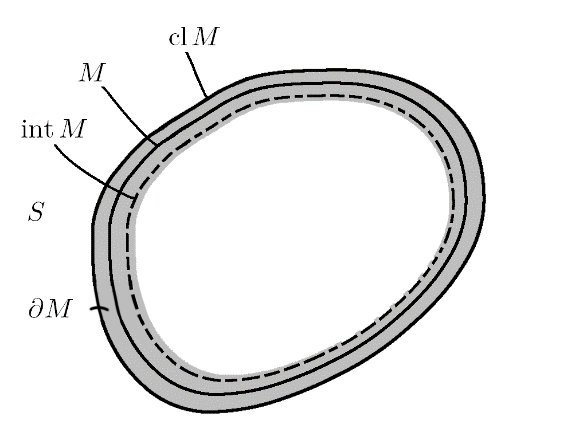
\includegraphics[width=76mm]{8.1.1.g.png}
\end{center}
\begin{thm}\label{8.1.1.16}
位相空間$\left( S,\mathfrak{O} \right)$において、$\forall M \in \mathfrak{P}(S)$に対し、次式が成り立つ\footnote{別の表記を用いれば、次のようになる。
\begin{align*}
  M^{a} &= M^{i} \sqcup M^{f}\\
  S &= M^{i} \sqcup M^{f} \sqcup M^{e}
\end{align*}}。
\begin{align*}
{\mathrm{cl}}M &= {\mathrm{int}}M \sqcup \partial M\\
S &= {\mathrm{int}}M \sqcup \partial M \sqcup {\mathrm{ext}}M
\end{align*}
\end{thm}
\begin{proof}
これらは定義より明らかである。実際、位相空間$\left( S,\mathfrak{O} \right)$が与えられ$M \in \mathfrak{P}(S)$なる集合$M$において、差集合の性質より${\mathrm{cl}}M = {\mathrm{int}}M \sqcup {\mathrm{cl}}M \setminus {\mathrm{int}}M = {\mathrm{int}}M \sqcup \partial M$が成り立ち、これと$S = {\mathrm{cl}}M \sqcup {\mathrm{ext}}M$が成り立つことにより、$S = {\mathrm{int}}M \sqcup \partial M \sqcup {\mathrm{ext}}M$が得られる。
\end{proof}
\begin{thm}\label{8.1.1.17}
位相空間$\left( S,\mathfrak{O} \right)$において、$\forall M \in \mathfrak{P}(S)$に対し、その集合$M$の境界$\partial(M)$は閉集合である。
\end{thm}
\begin{proof}
位相空間$\left( S,\mathfrak{O} \right)$とこれの閉集合系$\mathfrak{A}$、$M \in \mathfrak{P}(S)$なる集合$M$が与えられたとき、境界の定義より次のようになる。
\begin{align*}
S \setminus \partial M &= S \setminus \left( {\mathrm{cl}}M \setminus {\mathrm{int}}M \right)\\
&= S \setminus \left( {\mathrm{cl}}M \cap \left( S \setminus {\mathrm{int}}M \right) \right)\\
&= S \setminus {\mathrm{cl}}M \cup S \setminus S \setminus {\mathrm{int}}M\\
&= S \setminus {\mathrm{cl}}M \cup {\mathrm{int}}M
\end{align*}
ここで、${\mathrm{cl}}M\in \mathfrak{A}$が成り立つのであったので、閉集合の定義より$S \setminus {\mathrm{cl}}M\in \mathfrak{O}$が成り立つかつ、${\mathrm{int}}M\in \mathfrak{O}$が成り立つので、位相の定義より$S \setminus {\mathrm{cl}}M \cap {\mathrm{int}}M\in \mathfrak{O}$が成り立つ。したがって、$S \setminus \partial M \in \mathfrak{O}$が成り立ち閉集合の定義より$S \setminus \partial M$が成り立つ。
\end{proof}
\begin{thm}\label{8.1.1.18}
位相空間$\left( S,\mathfrak{O} \right)$において、$\forall M \in \mathfrak{P}(S)$に対し、その集合$M$が開集合であるならそのときに限り、積集合$M \cap \partial M$は空集合である、即ち、$M \in \mathfrak{O}$が成り立つならそのときに限り、$M \cap \partial M = \emptyset$が成り立つ。\par
これにより、開集合とはその集合自身の境界と交わらないような集合であることが分かる。
\end{thm}
\begin{proof}
位相空間$\left( S,\mathfrak{O} \right)$と$M \in \mathfrak{O}$なる集合$M$を考える。このとき、その集合$M$が開集合で$M = {\mathrm{int}}M$が成り立つので、したがって、$M \cap \partial M = \emptyset$が成り立つとすれば、
\begin{align*}
M \cap \partial M = \emptyset &\Leftrightarrow M \cap \left( {\mathrm{cl}}M \setminus {\mathrm{int}}M \right) = \emptyset\\
&\Leftrightarrow M \cap {\mathrm{cl}}M \cap S \setminus {\mathrm{int}}M = \emptyset\\
&\Leftrightarrow {\mathrm{cl}}M \cap M \cap S \setminus {\mathrm{int}}M = \emptyset\\
&\Leftrightarrow {\mathrm{cl}}M \cap M \cap S \setminus M = \emptyset\\
&\Leftrightarrow {\mathrm{cl}}M \cap \emptyset = \emptyset
\end{align*}
これは恒真式であるから、これより$M \in \mathfrak{O}$かつ$M \cap \partial M = \emptyset$は常に真であり、$M \in \mathfrak{O}$かつ$M \cap \partial M = \emptyset$が成り立つまたは$M \in \mathfrak{O}$、$M \cap \partial M = \emptyset$どちらも成り立たないということも真となりこれが同値にあたるので、$M \in \mathfrak{O}$が成り立つならそのときに限り、$M \cap \partial M = \emptyset$が成り立つことも真である。
\end{proof}
\begin{thm}\label{8.1.1.19}
位相空間$\left( S,\mathfrak{O} \right)$において、$\forall M \in \mathfrak{P}(S)$に対し、その集合$M$が閉集合であるならそのときに限り、その集合$M$はその境界$\partial M$を含む、即ち、その位相空間$\left( S,\mathfrak{O} \right)$の閉集合系を$\mathfrak{A}$として$M \in \mathfrak{A}$が成り立つならそのときに限り、$\partial M \subseteq M$が成り立つ。
\end{thm}
\begin{proof}
位相空間$\left( S,\mathfrak{O} \right)$とこれの閉集合系$\mathfrak{A}$、$M \in \mathfrak{A}$なる集合$M$を考える。このとき、閉集合の定義より$S \setminus M \in \mathfrak{O}$が成り立つので、${\mathrm{int}}(S \setminus M) = S \setminus M$が成り立ち$S \setminus {\mathrm{int}}(S \setminus M) = {\mathrm{cl}}M$より${\mathrm{cl}}M = M$が成り立つ。したがって、$\partial M \subseteq M$が成り立つとすれば、次式が成り立つ。
\begin{align*}
\partial M \subseteq M &\Leftrightarrow {\mathrm{cl}}M \setminus {\mathrm{int}}M \subseteq M\\
&\Leftrightarrow M \setminus {\mathrm{int}}M \subseteq M
\end{align*}
これは恒真式であるから、これより$M \in \mathfrak{A}$かつ$\partial M \subseteq M$は常に真であり、$M \in \mathfrak{A}$かつ$\partial M \subseteq M$が成り立つまたは$M \in \mathfrak{A}$、$\partial M \subseteq M$どちらも成り立たないということも真となりこれが同値にあたるので、$M \in \mathfrak{A}$が成り立つならそのときに限り、$\partial M \subseteq M$が成り立つことも真である。
\end{proof}
\begin{thm}\label{8.1.1.20}
位相空間$\left( S,\mathfrak{O} \right)$において、$\forall M \in \mathfrak{P}(S)$に対し、その集合$M$の境界点はその集合$M$の触点であるかつ、集合$S \setminus M$の触点でもある。
\end{thm}
\begin{proof}
位相空間$\left( S,\mathfrak{O} \right)$と$M \in \mathfrak{P}(S)$なる集合$M$が考えられれば、その集合$M$の位相的境界の定義より次のようになる。
\begin{align*}
a \in \partial M &= {\mathrm{cl}}M \setminus {\mathrm{int}}M\\
&= {\mathrm{cl}}M \cap \left( S \setminus {\mathrm{int}}M \right)\\
&= {\mathrm{cl}}M \cap {\mathrm{cl}}(S \setminus M)
\end{align*}
これが成り立つならそのときに限り、その元$a$はその集合$M$の触点であるかつ、集合$S \setminus M$の触点でもある。
\end{proof}
\begin{dfn}
位相空間$\left( S,\mathfrak{O} \right)$において、$\forall M \in \mathfrak{P}(S)$に対し、$a \in S$なる元$a$が集合$M \setminus \left\{ a \right\}$の触点であるとき、即ち、$a \in {\mathrm{cl}}\left( M \setminus \left\{ a \right\} \right)$が成り立つとき、その元$a$はその集合$M$の集積点という。
\end{dfn}
\begin{thm}\label{8.1.1.21}
位相空間$\left( S,\mathfrak{O} \right)$において、$\forall M \in \mathfrak{P}(S)$に対し、その集合$M$の集積点$a$はその集合$M$の触点の1つでもある。特に、$a \notin M$なるその集合$M$の全ての触点たち$a$はその集合$M$の集積点でもある。
\end{thm}
\begin{proof}
位相空間$\left( S,\mathfrak{O} \right)$が与えられ$M \in \mathfrak{P}(S)$なる任意の集合$M$とその集合$M$の集積点$a$において、$M \setminus \left\{ a \right\} \subseteq M$が成り立つので、${\mathrm{cl}}\left( M \setminus \left\{ a \right\} \right) \subseteq {\mathrm{cl}}M$が成り立つことにより、$a \in {\mathrm{cl}}M$が得られ、したがって、その集積点$a$はその集合$M$の触点の1つでもある。特に、$a \notin M$なるその集合$M$の任意の触点$a$について、$a \in {\mathrm{cl}}M$が成り立つかつ、$M \setminus \left\{ a \right\} = M$が成り立つので、$a \in {\mathrm{cl}}\left( M \setminus \left\{ a \right\} \right)$が成り立つ。
\end{proof}
\begin{dfn}
位相空間$\left( S,\mathfrak{O} \right)$において、$\forall M \in \mathfrak{P}(S)$に対し、$a \in M$なる元$a$でその集合$M$の集積点でないとき、その元$a$はその集合$M$の孤立点という。
\end{dfn}
%\hypertarget{ux8fd1ux508d}{%
\subsubsection{近傍}%\label{ux8fd1ux508d}}
\begin{dfn}
位相空間$\left( S,\mathfrak{O} \right)$において、$a \in S$なる元$a$が$V \in \mathfrak{P}(S)$なる集合$V$の内点である、即ち、$a \in {\mathrm{int}}V$が成り立つとき、その集合$V$がその元$a$の近傍であるという。
\end{dfn}\par
これは次の図のように考えると、分かりやすかろう。
\begin{center}
  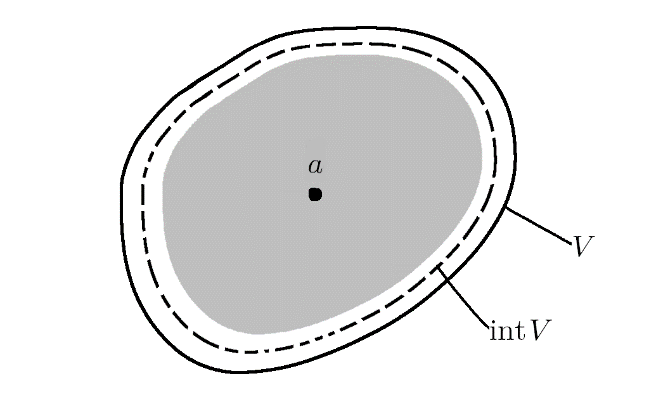
\includegraphics[width=74mm]{8.1.1.h.png}
\end{center}
\begin{dfn}
位相空間$\left( S,\mathfrak{O} \right)$において、$a \in S$なる元$a$の近傍全体の集合をその位相$\mathfrak{O}$におけるその元$a$の全近傍系といい、$\mathbf{V}(a)$などと書く、即ち、次式のように定義する。
\begin{align*}
\mathbf{V}(a) = \left\{ V \in \mathfrak{P}(S) \middle| a \in {\mathrm{int}}V \right\}
\end{align*}
\end{dfn}
\begin{thm}\label{8.1.1.22}
位相空間$\left( S,\mathfrak{O} \right)$において、$\forall a \in S$に対し、$V \in \mathbf{V}(a)$が成り立つならそのときに限り、$\exists O \in \mathfrak{O}$に対し、$a \in O \subseteq V$が成り立つ。
\end{thm}\par
これは次の図のように考えると、分かりやすかろう。
\begin{center}
  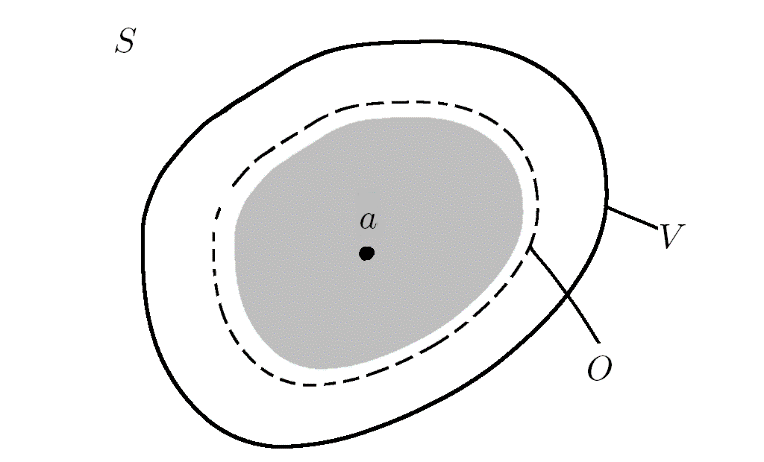
\includegraphics[width=88mm]{8.1.1.i.PNG}
\end{center}
\begin{proof}
位相空間$\left( S,\mathfrak{O} \right)$において、$\forall a \in S$に対し、$V \in \mathbf{V}(a)$が成り立つなら、開核と近傍の定義より$a \in {\mathrm{int}}V \subseteq V$が成り立つ。逆に、$a \in {\mathrm{int}}V$が成り立たないとき、$\exists O \in \mathfrak{O}$に対し、$a \in O \subseteq V$が成り立つ仮定すると、$a \in O = {\mathrm{int}}O \subseteq {\mathrm{int}}V$が得られるが、これは矛盾している。ゆえに、$a \in {\mathrm{int}}V$が成り立たないなら、$\forall O \in \mathfrak{O}$に対し、$a \notin O$が成り立つ、または、$O \subseteq V$が成り立たない。したがって、対偶律より$\exists O \in \mathfrak{O}$に対し、$a \in O \subseteq V$が成り立つなら、$V \in \mathbf{V}(a)$が成り立つ。
\end{proof}
\begin{thm}\label{8.1.1.23}
位相空間$\left( S,\mathfrak{O} \right)$において、$O \in \mathfrak{O}$が成り立つならそのときに限り、$\forall a \in O$に対し、$O \in \mathbf{V}(a)$が成り立つ。
これは次の図のように考えると、分かりやすかろう。
\begin{center}
  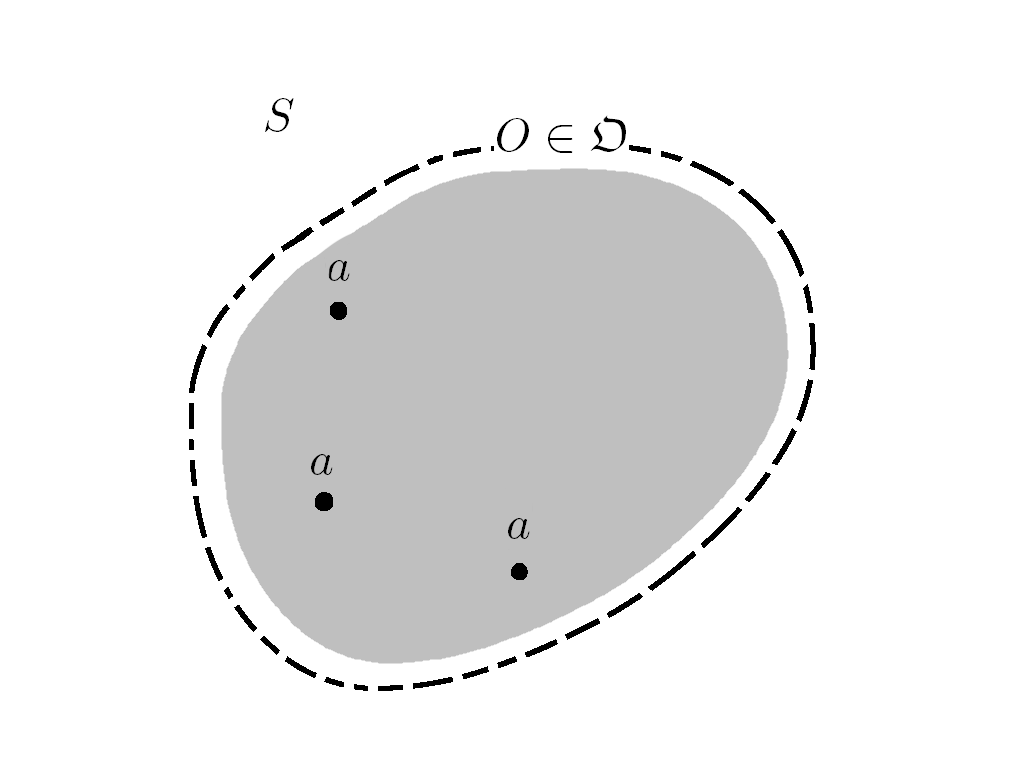
\includegraphics[width=92mm]{8.1.1.j.PNG}
\end{center}
\end{thm}
\begin{proof}
位相空間$\left( S,\mathfrak{O} \right)$において、$O \in \mathfrak{O}$が成り立つなら、$O = {\mathrm{int}}O$が成り立つので、$\forall a \in O$に対し、$a \in O = {\mathrm{int}}O$が成り立つ、即ち、$O \in \mathbf{V}(a)$が成り立つ。逆に、$\forall a \in O$に対し、$O \in \mathbf{V}(a)$が成り立つ、即ち、$a \in {\mathrm{int}}O$が成り立つなら、$O \subseteq {\mathrm{int}}O$が得られることになり、${\mathrm{int}}O \subseteq O$が成り立つので、$O = {\mathrm{int}}O$が成り立つ。これが成り立つならそのときに限り、その集合$O$は開集合である、即ち、$O \in \mathfrak{O}$が成り立つ。
\end{proof}
\begin{thm}\label{8.1.1.24}
位相空間$\left( S,\mathfrak{O} \right)$が与えられたとき、$\forall a \in S$に対し、その元$a$の全近傍系$\mathbf{V}(a)$について、次のことが成り立つ。
\begin{itemize}
\item
  $\forall V \in \mathbf{V}(a)$に対し、$a \in V$が成り立つ。
\item
  $\forall V \in \mathbf{V}(a)\forall W \in \mathfrak{P}(S)$に対し、$V \subseteq W$が成り立つなら、$W \in \mathbf{V}(a)$が成り立つ。
\item
  $\forall V,W \in \mathbf{V}(a)$に対し、$V \cap W \in \mathbf{V}(a)$が成り立つ。
\item
  $\forall V \in \mathbf{V}(a)\exists W \in \mathbf{V}(a)\forall b \in W$に対し、$V \in \mathbf{V}(b)$が成り立つ\footnote{例えば、$W = {\mathrm{int}}(V)$が挙げられる。}。
\end{itemize}
\end{thm}
これらの主張は次の図のように考えると、分かりやすかろう。
\begin{center}
  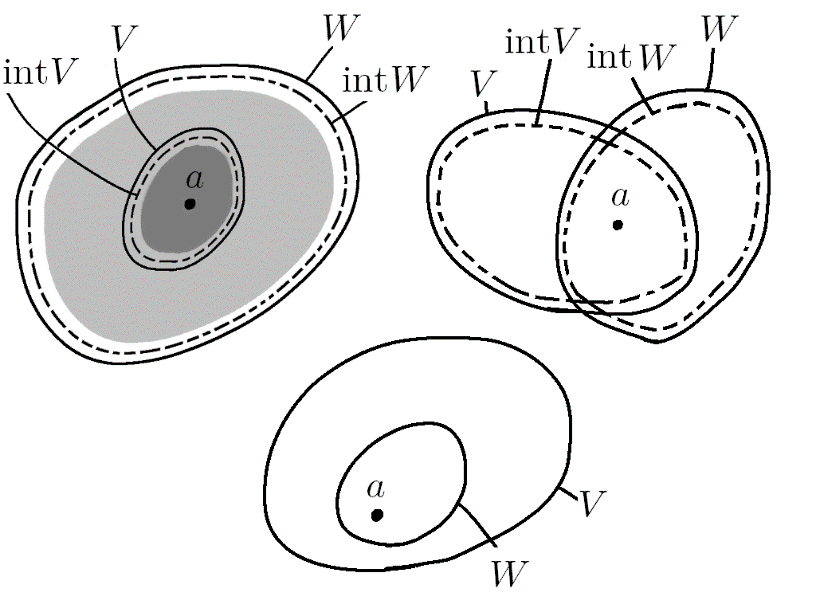
\includegraphics[width=94mm]{8.1.1.k.png}
\end{center}
\begin{proof}
位相空間$\left( S,\mathfrak{O} \right)$と$a \in S$なる元$a$の全近傍系$\mathbf{V}(a)$において、$\forall V \in \mathbf{V}(a)$に対し、定義より$a \in {\mathrm{int}}V$が成り立ち、${\mathrm{int}}V \subseteq V$が成り立つので、$a \in {\mathrm{int}}V \subseteq V$が得られる。よって、$a \in V$が成り立つ。\par
また、$\forall V \in \mathbf{V}(a)\forall W \in \mathfrak{P}(S)$に対し$V \subseteq W$が成り立つなら、定義より$a \in {\mathrm{int}}V$が成り立ち、${\mathrm{int}}V \subseteq V$が成り立つかつ、仮定より$V \subseteq W$が成り立つことより${\mathrm{int}}V \subseteq {\mathrm{int}}W$が成り立つので、$a \in {\mathrm{int}}V \subseteq {\mathrm{int}}W$が得られる。よって、$W \in \mathbf{V}(a)$が成り立つ。\par
$\forall V,W \in \mathbf{V}(a)$に対し、定義より$a \in {\mathrm{int}}V$かつ$a \in {\mathrm{int}}W$が成り立ち、したがって、$a \in {\mathrm{int}}V \cap {\mathrm{int}}W = {\mathrm{int}}(V \cap W)$が成り立つ。よって、$V \cap W \in \mathbf{V}(a)$が成り立つ。\par
$\forall V \in \mathbf{V}(a)$に対し、$W = {\mathrm{int}}V$とおけば、$\forall b \in W$に対し、$b \in W = {\mathrm{int}}V$が成り立つので、定義より$V \in \mathbf{V}(b)$が得られるかつ、$\forall a \in {\mathrm{int}}V$に対し、$a \in {\mathrm{int}}V = {\mathrm{int}}{{\mathrm{int}}V}$が成り立つので、定義より$W = {\mathrm{int}}V \in \mathbf{V}(a)$が成り立つ。よって、$\forall V \in \mathbf{V}(a)\exists W \in \mathbf{V}(a)\forall b \in W$に対し、$V \in \mathbf{V}(b)$が成り立つ。
\end{proof}
\begin{thm}\label{8.1.1.25}
空集合$\emptyset$でない集合$S$を用いて$a \in S$なる元々$a$に対するそれぞれ1つづつの空集合$\emptyset$でない集合$\mathfrak{P}(S)$の部分集合たち$\mathbf{V}(a)$が次のことが成り立つとする。
\begin{itemize}
\item
  $\forall V \in \mathbf{V}(a)$に対し、$a \in V$が成り立つ。
\item
  $\forall V \in \mathbf{V}(a)\forall W \in \mathfrak{P}(S)$に対し、$V \subseteq W$が成り立つなら、$W \in \mathbf{V}(a)$が成り立つ。
\item
  $\forall V,W \in \mathbf{V}(a)$に対し、$V \cap W \in \mathbf{V}(a)$が成り立つ。
\item
  $\forall V \in \mathbf{V}(a)\exists W \in \mathbf{V}(a)\forall b \in W$に対し、$V \in \mathbf{V}(b)$が成り立つ。
\end{itemize}
このとき、その集合$\mathbf{V}(a)$が位相空間$\left( S,\mathfrak{O} \right)$における$a \in S$なる元々$a$の全近傍系と一致できる1つの位相$\mathfrak{O}$がただ1つに決まり、次式のように与えられる。
\begin{align*}
\mathfrak{O}=\left\{ M \in \mathfrak{P}(S) \middle| a \in M \Rightarrow M \in \mathbf{V}(a) \right\}
\end{align*}
\end{thm}\par
これを位相の公理とするときがありこのような公理を全近傍系の公理という\footnote{もしかしたらぼくが一番好きな位相空間の公理かもしれません…。}。
\begin{proof}
空集合$\emptyset$でない集合$S$を用いて$a \in S$なる元々$a$に対するそれぞれ1つづつの空集合$\emptyset$でない集合$\mathfrak{P}(S)$の部分集合たち$\mathbf{V}(a)$が次のことが成り立つとする。
\begin{itemize}
\item
  $\forall V \in \mathbf{V}(a)$に対し、$a \in V$が成り立つ。
\item
  $\forall V \in \mathbf{V}(a)\forall W \in \mathfrak{P}(S)$に対し、$V \subseteq W$が成り立つなら、$W \in \mathbf{V}(a)$が成り立つ。
\item
  $\forall V,W \in \mathbf{V}(a)$に対し、$V \cap W \in \mathbf{V}(a)$が成り立つ。
\item
  $\forall V \in \mathbf{V}(a)\exists W \in \mathbf{V}(a)\forall b \in W$に対し、$V \in \mathbf{V}(b)$が成り立つ。
\end{itemize}
ここで、$\mathfrak{O}=\left\{ M \in \mathfrak{P}(S) \middle| a \in M \Rightarrow M \in \mathbf{V}(a) \right\}$なる集合$\mathfrak{O}$が位相空間$\left( S,\mathfrak{O} \right)$における位相に、その集合$\mathbf{V}(a)$が$a \in S$なる元$a$の全近傍系に一致することを示そう。\par
$\forall a \in S$に対し、仮定より$\exists V \in \mathbf{V}(a)$が成り立ち、その集合$\mathbf{V}(a)$がその集合$\mathfrak{P}(S)$の部分集合であるから、$V \subseteq S$が成り立つ。これにより、$S \in \mathbf{V}(a)$が成り立つ。また、明らかに$\mathfrak{\emptyset \in O}$が成り立つ。\par
$\forall O,P \in \mathfrak{O}$に対し、$O \cap P = \emptyset$が成り立つなら、上記より$O \cap P \in \mathfrak{O}$が成り立つ。$O \cap P \neq \emptyset$が成り立つなら、$\forall a \in S$に対し、$a \in O \cap P$が成り立つとき、その集合$\mathfrak{O}$の定義より$a \in O$が成り立つなら、$O \in \mathbf{V}(a)$が成り立つかつ、$a \in P$が成り立つなら、$P \in \mathbf{V}(a)$が成り立つので、$O,P \in \mathbf{V}(a)$が成り立つなら、$O \cap P \in \mathbf{V}(a)$が成り立ち、よって、$O \cap P \in \mathfrak{O}$が成り立つ。\par
任意の添数集合$\varLambda$によって添数づけられたその集合$\mathfrak{O}$の元の族$\left\{ O_{\lambda} \right\}_{\lambda \in \varLambda}$において、$\bigcup_{\lambda \in \varLambda} O_{\lambda} = \emptyset$が成り立つなら、上記より$\bigcup_{\lambda \in \varLambda} O_{\lambda}\in \mathfrak{O}$が成り立つ。$\bigcup_{\lambda \in \varLambda} O_{\lambda} \neq \emptyset$が成り立つなら、$\forall a \in S$に対し、$a \in \bigcup_{\lambda \in \varLambda} O_{\lambda}$が成り立つとき、$a \in O_{\lambda'}$なるその添数集合$\varLambda$の元$\lambda'$が存在して、$O_{\lambda'} \in \mathbf{V}(a)$が成り立つ。$O_{\lambda'} \subseteq \bigcup_{\lambda \in \varLambda} O_{\lambda}$が成り立つので、$\bigcup_{\lambda \in \varLambda} O_{\lambda} \in \mathbf{V}(a)$が成り立つ。よって、$\bigcup_{\lambda \in \varLambda} O_{\lambda}\in \mathfrak{O}$が成り立つ。\par
以上より次の条件たちが満たされその集合$\mathfrak{O}$は位相に相当する。
\begin{itemize}
\item
  $S,\emptyset \in \mathfrak{O}$が成り立つ。
\item
  $\forall O,P \in \mathfrak{O}$に対し、$O \cap P \in \mathfrak{O}$が成り立つ。
\item
  任意の添数集合$\varLambda$によって添数づけられたその集合$\mathfrak{O}$の元の族$\left\{ O_{\lambda} \right\}_{\lambda \in \varLambda}$において$\bigcup_{\lambda \in \varLambda} O_{\lambda}\in \mathfrak{O}$が成り立つ。
\end{itemize}\par
また、$S' = {\mathrm{int}}M$が成り立つことを次のこといづれも成り立つことと定め
\begin{itemize}
\item
  $S' \subseteq M$が成り立つ。
\item
  $S'\in \mathfrak{O}$が成り立つ。
\item
  $O \subseteq M$かつ$O \in \mathfrak{O}$が成り立つなら、$O \subseteq S'$が成り立つ。
\end{itemize}
$a \in {\mathrm{int}}V \Leftrightarrow V \in \mathbf{V}(a)$が成り立つことを示そう。\par
このとき、${\mathrm{int}}V\in \mathfrak{O}$が成り立つので、$a \in {\mathrm{int}}V \Rightarrow {\mathrm{int}}V \in \mathbf{V}(a)$が成り立ち、${\mathrm{int}}V \subseteq V$が成り立つので、以上より、$a \in {\mathrm{int}}V \Rightarrow V \in \mathbf{V}(a)$が成り立つ。\par
逆に、$\forall a \in S\forall V \in \mathbf{V}(a)$に対し、$U = \left\{ b \in S \middle| V \in \mathbf{V}(b) \right\}$なる集合$U$を考えよう。$b \in U$が成り立つなら、$V \in \mathbf{V}(b)$が得られ、したがって、$b \in V$が成り立つので、$U \subseteq V$が得られる。$\forall b \in U$に対し、$V \in \mathbf{V}(b)$が成り立ち、$\exists W \in \mathbf{V}(b)\forall c \in W$に対し、$V \in \mathbf{V}(c)$が成り立つのであったので、定義より$c \in U$が成り立ち$W \subseteq U$が得られ、$W \in \mathbf{V}(b)$より$W \subseteq U$が成り立つなら、$U \in \mathbf{V}(b)$が成り立つので、$b \in U \Rightarrow U \in \mathbf{V}(b)$が得られ、したがって、$U \in \mathfrak{O}$が成り立つ。$O \subseteq V$かつ$O \in \mathfrak{O}$が成り立つなら、$\forall d \in O$に対し、$O \in \mathbf{V}(d)$が成り立ち、したがって、$V \in \mathbf{V}(d)$が成り立つので、$d \in U$が成り立つ。したがって、$d \in O \Rightarrow d \in U$が得られ$O \subseteq U$が成り立つ。以上より、$U \subseteq V$かつ$U \in \mathfrak{O}$が成り立つかつ、$O \subseteq V$かつ$O \in \mathfrak{O}$が成り立つなら、$O \subseteq U$が成り立つので、$U = {\mathrm{int}}V$が成り立ち$V \in \mathbf{V}(a)$が成り立つなら、$a \in \left\{ b \in S \middle| V \in \mathbf{V}(b) \right\} = {\mathrm{int}}V$が得られ、したがって、$V \in \mathbf{V}(a) \Rightarrow a \in {\mathrm{int}}V$が成り立つ。\par
以上より、$a \in {\mathrm{int}}V \Leftrightarrow V \in \mathbf{V}(a)$が成り立つことが示された。
\end{proof}
\begin{thm}\label{8.1.1.26}
位相空間$\left( S,\mathfrak{O} \right)$において$\forall a \in S$に対し、その元$a$の1つの全近傍系$\mathbf{V}(a)$が与えられたとき、$\forall M \in \mathfrak{P}(S)$に対し、次のことが成り立つ。
\begin{itemize}
\item
  $a \in {\mathrm{int}}M$が成り立つならそのときに限り、$\exists V \in \mathbf{V}(a)$に対し、$V \subseteq M$が成り立つ。
\item
  $a \in {\mathrm{ext}}M$が成り立つならそのときに限り、$\exists V \in \mathbf{V}(a)$に対し、$V \cap M = \emptyset$が成り立つ。
\item
  $a \in {\mathrm{cl}}M$が成り立つならそのときに限り、$\forall V \in \mathbf{V}(a)$に対し、$V \cap M \neq \emptyset$が成り立つ。
\item
  $a \in \partial M$が成り立つならそのときに限り、$\forall V \in \mathbf{V}(a)$に対し、$V \cap M \neq \emptyset$かつ$V \cap S \setminus M \neq \emptyset$が成り立つ。
\end{itemize}
\end{thm}
\begin{proof}
位相空間$\left( S,\mathfrak{O} \right)$において$\forall a \in S$に対し、その元$a$の1つの全近傍系$\mathbf{V}(a)$が与えられたとき、$\forall M \in \mathfrak{P}(S)$に対し、$a \in {\mathrm{int}}M$が成り立つなら、$M \in \mathbf{V}(a)$より明らかに$\exists V \in \mathbf{V}(a)$に対し、$V \subseteq M$が成り立つ。逆に、$\exists V \in \mathbf{V}(a)$に対し、$V \subseteq M$が成り立つなら、$a \in {\mathrm{int}}V$が成り立つかつ${\mathrm{int}}V \subseteq {\mathrm{int}}M$が成り立つので、$a \in {\mathrm{int}}M$が得られる。\par
$a \in {\mathrm{ext}}M = {\mathrm{int}}(S \setminus M)$が成り立つならそのときに限り、上記の議論により$\exists V \in \mathbf{V}(a)$に対し、$V \subseteq S \setminus M$が成り立つ。このとき、次のようになることから、
\begin{align*}
V \subseteq S \setminus M &\Leftrightarrow \forall a \in S[ a \in V \Rightarrow a \in S \setminus M]\\
&\Leftrightarrow \forall a \in S\left[ a \notin V \vee (a \in S \land a \notin M) \right]\\
&\Leftrightarrow \forall a \in S\left[ (a \notin V \vee a \in S) \land (a \notin V \vee a \notin M) \right]\\
&\Leftrightarrow \forall a \in S[ a \notin V \vee a \in S] \land \forall a \in S\left[ \neg(a \in V \land a \in M) \right]\\
&\Leftrightarrow \forall a \in S[ a \in V \Rightarrow a \in S] \land \neg\exists a \in S[ a \in V \cap M]\\
&\Leftrightarrow V \subseteq S \land V \cap M = \emptyset\\
&\Leftrightarrow V \cap M = \emptyset
\end{align*}
これが成り立つならそのときに限り、$\exists V \in \mathbf{V}(a)$に対し、$V \cap M = \emptyset$が成り立つ。\par
$a \in {\mathrm{cl}}M$が成り立つならそのときに限り、$a \in S \setminus {\mathrm{int}}(S \setminus M)$が成り立つ、即ち、$a \notin {\mathrm{int}}(S \setminus M)$が成り立つ。そこで、上記の議論によりこれが成り立つならそのときに限り、$\forall V \in \mathbf{V}(a)$に対し、$V \cap M \neq \emptyset$が成り立つ。\par
$a \in \partial M$が成り立つならそのときに限り、$a \in {\mathrm{cl}}M$が成り立つかつ、$a \notin {\mathrm{int}}M$が成り立つ。これが成り立つならそのときに限り、上記の議論により、$\forall V \in \mathbf{V}(a)$に対し、$V \cap M \neq \emptyset$が成り立つかつ、$\forall V \in \mathbf{V}(a)$に対し、$V \subseteq M$が成り立たない。このとき、次のようになることから、
\begin{align*}
\neg V \subseteq M &\Leftrightarrow \neg\forall a \in S[ a \in V \Rightarrow a \in M]\\
&\Leftrightarrow \exists a \in S\left[ \neg(a \notin V \vee a \in M) \right]\\
&\Leftrightarrow \exists a \in S[ a \in V \land a \notin M]\\
&\Leftrightarrow \exists a \in S[ a \in V \land a \in S \setminus M]\\
&\Leftrightarrow \exists a \in S[ a \in V \cap S \setminus M]\\
&\Leftrightarrow V \cap S \setminus M \neq \emptyset
\end{align*}
これが成り立つならそのときに限り、$\forall V \in \mathbf{V}(a)$に対し、$V \cap M \neq \emptyset$が成り立つかつ、$\forall V \in \mathbf{V}(a)$に対し、$V \cap S \setminus M \neq \emptyset$が成り立つ、即ち、$\forall V \in \mathbf{V}(a)$に対し、$V \cap M \neq \emptyset$かつ$V \cap S \setminus M \neq \emptyset$が成り立つ。
\end{proof}
\begin{thebibliography}{50}
\bibitem{1}
  松坂和夫, 集合・位相入門, 岩波書店, 1968. 新装版第2刷 p152-165 ISBN978-4-00-029871-1
\bibitem{2}
  川平友規. "第3章 位相空間の基礎のキソ". 一橋大学. \url{http://www.math.titech.ac.jp/~kawahira/courses/kiso/03-isou.pdf} (2021-1-10 取得)
\bibitem{3}
  きいねく. "大学数学の難関分野:【位相空間論】とは一体何なのか?". note. \url{https://note.com/keyneqq/n/na8d370a26bff} (2022-3-26 18:04 閲覧)
\bibitem{4}
  桂田祐史. "数学解析 第11回~開集合と閉集合(1)~". 明治大学. \url{http://nalab.mind.meiji.ac.jp/~mk/lecture/kaiseki-2021/K11_0628_handout.pdf} (2022-3-26 18:12 取得)
\end{thebibliography}
\end{document}

\clearpage
\documentclass[dvipdfmx]{jsarticle}
\setcounter{section}{1}
\setcounter{subsection}{1}
\usepackage{xr}
\externaldocument{8.1.1}
\usepackage{amsmath,amsfonts,amssymb,array,comment,mathtools,url,docmute}
\usepackage{longtable,booktabs,dcolumn,tabularx,mathtools,multirow,colortbl,xcolor}
\usepackage[dvipdfmx]{graphics}
\usepackage{bmpsize}
\usepackage{amsthm}
\usepackage{enumitem}
\setlistdepth{20}
\renewlist{itemize}{itemize}{20}
\setlist[itemize]{label=•}
\renewlist{enumerate}{enumerate}{20}
\setlist[enumerate]{label=\arabic*.}
\setcounter{MaxMatrixCols}{20}
\setcounter{tocdepth}{3}
\newcommand{\rotin}{\text{\rotatebox[origin=c]{90}{$\in $}}}
\newcommand{\amap}[6]{\text{\raisebox{-0.7cm}{\begin{tikzpicture} 
  \node (a) at (0, 1) {$\textstyle{#2}$};
  \node (b) at (#6, 1) {$\textstyle{#3}$};
  \node (c) at (0, 0) {$\textstyle{#4}$};
  \node (d) at (#6, 0) {$\textstyle{#5}$};
  \node (x) at (0, 0.5) {$\rotin $};
  \node (x) at (#6, 0.5) {$\rotin $};
  \draw[->] (a) to node[xshift=0pt, yshift=7pt] {$\textstyle{\scriptstyle{#1}}$} (b);
  \draw[|->] (c) to node[xshift=0pt, yshift=7pt] {$\textstyle{\scriptstyle{#1}}$} (d);
\end{tikzpicture}}}}
\newcommand{\twomaps}[9]{\text{\raisebox{-0.7cm}{\begin{tikzpicture} 
  \node (a) at (0, 1) {$\textstyle{#3}$};
  \node (b) at (#9, 1) {$\textstyle{#4}$};
  \node (c) at (#9+#9, 1) {$\textstyle{#5}$};
  \node (d) at (0, 0) {$\textstyle{#6}$};
  \node (e) at (#9, 0) {$\textstyle{#7}$};
  \node (f) at (#9+#9, 0) {$\textstyle{#8}$};
  \node (x) at (0, 0.5) {$\rotin $};
  \node (x) at (#9, 0.5) {$\rotin $};
  \node (x) at (#9+#9, 0.5) {$\rotin $};
  \draw[->] (a) to node[xshift=0pt, yshift=7pt] {$\textstyle{\scriptstyle{#1}}$} (b);
  \draw[|->] (d) to node[xshift=0pt, yshift=7pt] {$\textstyle{\scriptstyle{#2}}$} (e);
  \draw[->] (b) to node[xshift=0pt, yshift=7pt] {$\textstyle{\scriptstyle{#1}}$} (c);
  \draw[|->] (e) to node[xshift=0pt, yshift=7pt] {$\textstyle{\scriptstyle{#2}}$} (f);
\end{tikzpicture}}}}
\renewcommand{\thesection}{第\arabic{section}部}
\renewcommand{\thesubsection}{\arabic{section}.\arabic{subsection}}
\renewcommand{\thesubsubsection}{\arabic{section}.\arabic{subsection}.\arabic{subsubsection}}
\everymath{\displaystyle}
\allowdisplaybreaks[4]
\usepackage{vtable}
\theoremstyle{definition}
\newtheorem{thm}{定理}[subsection]
\newtheorem*{thm*}{定理}
\newtheorem{dfn}{定義}[subsection]
\newtheorem*{dfn*}{定義}
\newtheorem{axs}[dfn]{公理}
\newtheorem*{axs*}{公理}
\renewcommand{\headfont}{\bfseries}
\makeatletter
  \renewcommand{\section}{%
    \@startsection{section}{1}{\z@}%
    {\Cvs}{\Cvs}%
    {\normalfont\huge\headfont\raggedright}}
\makeatother
\makeatletter
  \renewcommand{\subsection}{%
    \@startsection{subsection}{2}{\z@}%
    {0.5\Cvs}{0.5\Cvs}%
    {\normalfont\LARGE\headfont\raggedright}}
\makeatother
\makeatletter
  \renewcommand{\subsubsection}{%
    \@startsection{subsubsection}{3}{\z@}%
    {0.4\Cvs}{0.4\Cvs}%
    {\normalfont\Large\headfont\raggedright}}
\makeatother
\makeatletter
\renewenvironment{proof}[1][\proofname]{\par
  \pushQED{\qed}%
  \normalfont \topsep6\p@\@plus6\p@\relax
  \trivlist
  \item\relax
  {
  #1\@addpunct{.}}\hspace\labelsep\ignorespaces
}{%
  \popQED\endtrivlist\@endpefalse
}
\makeatother
\renewcommand{\proofname}{\textbf{証明}}
\usepackage{tikz,graphics}
\usepackage[dvipdfmx]{hyperref}
\usepackage{pxjahyper}
\hypersetup{
 setpagesize=false,
 bookmarks=true,
 bookmarksdepth=tocdepth,
 bookmarksnumbered=true,
 colorlinks=false,
 pdftitle={},
 pdfsubject={},
 pdfauthor={},
 pdfkeywords={}}
\begin{document}
%\hypertarget{ux958bux57fa}{%
\subsection{開基}%\label{ux958bux57fa}}
%\hypertarget{ux4f4dux76f8ux306eux5f37ux5f31}{%
\subsubsection{位相の強弱}%\label{ux4f4dux76f8ux306eux5f37ux5f31}}
\begin{dfn}
1つの空集合でない集合$S$における2つの位相たち$\mathfrak{O}$、$\mathfrak{P}$が$\mathfrak{O \subseteq P}$を満たすとき、その位相$\mathfrak{O}$はその位相$\mathfrak{P}$より弱い、その位相$\mathfrak{P}$はその位相$\mathfrak{O}$より強いなどという。以上のように定義されることができるその集合$S$における位相たち全体の集合を$\mathcal{T}(S)$としよう。
\end{dfn}
\begin{thm}\label{8.1.2.1}
この組$\left( \mathcal{T}(S), \subseteq \right)$は明らかに順序集合をなす。
\end{thm}\par
ただし、全順序集合ではないことを注意されたい。
\begin{proof} 順序集合の公理にあてはめれば、直ちに示される。
\end{proof}
\begin{thm}\label{8.1.2.2} また、明らかに次式が成り立つ。
\begin{align*}
\min{\mathcal{T}(S)} &= \mathfrak{O}_{*} = \left\{ \emptyset,S \right\}\\
\max{\mathcal{T}(S)} &= \mathfrak{O}^{*} = \mathfrak{P}(S)
\end{align*}
\end{thm}
\begin{proof}
位相の公理より任意の位相$\mathfrak{O}$はその集合$\mathfrak{P}(S)$の部分集合であるかつ、$\mathfrak{O \subset}\left\{ \emptyset,S \right\}$なる位相$\mathfrak{O}$が存在すれば、これは位相の公理を満たさない。背理法により任意の位相$\mathfrak{O}$に対し、$\left\{ \emptyset,S \right\}\subseteq \mathfrak{O}$が成り立つ。これにより、示すべきことが示される。
\end{proof}
\begin{thm}\label{8.1.2.3}
それらの位相たち$\mathfrak{O}$、$\mathfrak{P}$から定まる閉集合系たちをそれぞれ$\mathfrak{A}$、$\mathfrak{B}$、全近傍系をそれぞれ$\mathbf{V}(a)$、$\mathbf{W}(a)$とおくと、次のことは同値である。
\begin{itemize}
\item
  $\mathfrak{O \subseteq P}$が成り立つ。
\item
  $\mathfrak{A \subseteq B}$が成り立つ。
\item
  $\forall a \in S$に対し、$\mathbf{V}(a) \subseteq \mathbf{W}(a)$が成り立つ。
\end{itemize}
\end{thm}
\begin{proof}
1つの空集合でない集合$S$における2つの位相たち$\mathfrak{O}$、$\mathfrak{P}$が$\mathfrak{O \subseteq P}$を満たすならそのときに限り、$\forall O \in \mathfrak{O}$に対し、$O \in \mathfrak{O}$が成り立つなら、$O \in \mathfrak{P}$が成り立つ。ここで、その集合$O$が$S \setminus A$と書き換えられると、それらの位相たち$\mathfrak{O}$、$\mathfrak{P}$から定まる閉集合系たちをそれぞれ$\mathfrak{A}$、$\mathfrak{B}$とおいて、$\forall A \in \mathfrak{A}$に対し、$A \in \mathfrak{A}$が成り立つなら、$A \in \mathfrak{B}$が成り立つので、これが成り立つならそのときに限り、$\mathfrak{A \subseteq B}$が成り立つ。以上より、次のことは同値であることが示された。
\begin{itemize}
\item
  $\mathfrak{O \subseteq P}$が成り立つ。
\item
  $\mathfrak{A \subseteq B}$が成り立つ。
\end{itemize}\par
また、それらの位相たち$\mathfrak{O}$、$\mathfrak{P}$が$\mathfrak{O \subseteq P}$を満たすとき、$\forall a \in S$に対し、全近傍系をそれぞれ$\mathbf{V}(a)$、$\mathbf{W}(a)$とおくと、$V \in \mathbf{V}(a)$が成り立つなら、定義より明らかに$\exists O \in \mathfrak{O}$に対し、$a \in O$かつ$O \subseteq V$が成り立ち、$\mathfrak{O \subseteq P}$が成り立つことに注意すれば、$O \in \mathfrak{P}$が成り立ち、これにより、$V \in \mathbf{W}(a)$が成り立つ。ゆえに、$\mathbf{V}(a) \subseteq \mathbf{W}(a)$が得られる。逆に、$\forall a \in S$に対し、$\mathbf{V}(a) \subseteq \mathbf{W}(a)$が成り立つとき、$\forall O \in \mathfrak{O}$に対し、$O \in \mathfrak{O}$が成り立つならそのときに限り、$\forall a \in O$に対し、$a \in {\mathrm{int}}O$が成り立つので、$a \in O$が成り立つなら、$O \in \mathbf{V}(a)$が成り立ち、したがって、$O \in \mathbf{W}(a)$が成り立つ。これにより、$O \in \mathfrak{P}$が成り立つ。以上より、$\mathfrak{O \subseteq P}$が得られた。以上の議論により、次のことは同値であることが示された。
\begin{itemize}
\item
  $\mathfrak{O \subseteq P}$が成り立つ。
\item
  $\forall a \in S$に対し、$\mathbf{V}(a) \subseteq \mathbf{W}(a)$が成り立つ。
\end{itemize}
\end{proof}
\begin{thm}\label{8.1.2.4}
その集合$\mathcal{T}(S)$の任意の元の族$\left\{ \mathfrak{O}_{\lambda} \right\}_{\lambda \in \varLambda}$が与えられたとき、その集合$\left\{ \mathfrak{O}_{\lambda} \right\}_{\lambda \in \varLambda}$の上限$\sup\left\{ \mathfrak{O}_{\lambda} \right\}_{\lambda \in \varLambda}と下限\inf\left\{ \mathfrak{O}_{\lambda} \right\}_{\lambda \in \varLambda}がその集合\mathcal{T}(S)$に存在する。しかも、次式が成り立つ。
\begin{align*}
\sup\left\{ \mathfrak{O}_{\lambda} \right\}_{\lambda \in \varLambda} &= \bigcap_{\scriptsize \begin{matrix}
\mathfrak{O \in}\mathcal{T}(S) \\
\bigcup_{\lambda \in \varLambda} \mathfrak{O}_{\lambda}\subseteq \mathfrak{O} \\
\end{matrix}} \mathfrak{O}\\
\inf\left\{ \mathfrak{O}_{\lambda} \right\}_{\lambda \in \varLambda} &= \bigcap_{\lambda \in \varLambda} \mathfrak{O}_{\lambda}
\end{align*}
\end{thm}\par
ここで、その集合$\bigcup_{\lambda \in \varLambda} \mathfrak{O}_{\lambda}$は必ずしもその集合$S$における位相となるとは限らないことに注意されたい。例えば、$S = \left\{ a,b,c \right\}$、$\mathfrak{O} = \left\{ \emptyset,\left\{ a \right\},S \right\}$、$\mathfrak{P} = \left\{ \emptyset,\left\{ b \right\},S \right\}$が与えられたとき、それらの集合たち$\mathfrak{O}$、$\mathfrak{P}$は位相となるが、$\left\{ a \right\} \cup \left\{ b \right\} \notin \mathfrak{O} \cup \mathfrak{P}$が成り立つので、その集合$\mathfrak{O \cup P}$は位相ではない。
\begin{proof}
その集合$S$における位相たち全体の集合$\mathcal{T}(S)$の任意の元の族$\left\{ \mathfrak{O}_{\lambda} \right\}_{\lambda \in \varLambda}$が与えられたとき、明らかに$\forall\lambda \in \varLambda$に対し、$\mathfrak{O}_{\lambda}\subseteq \mathfrak{P}(S)$が成り立つので、順序集合$\left( \left\{ \mathfrak{O}_{\lambda} \right\}_{\lambda \in \varLambda}, \subseteq \right)$は上に有界であり、その順序集合$\left( \left\{ \mathfrak{O}_{\lambda} \right\}_{\lambda \in \varLambda}, \subseteq \right)$の上界全体の集合を$U\left( \left\{ \mathfrak{O}_{\lambda} \right\}_{\lambda \in \varLambda} \right)$とおくと、$\mathfrak{\forall O \in}U\left( \left\{ \mathfrak{O}_{\lambda} \right\}_{\lambda \in \varLambda} \right)\forall\lambda \in \varLambda$に対し、$\mathfrak{O}_{\lambda}\subseteq \mathfrak{O}$が成り立つことになり、これが成り立つならそのときに限り、$\mathfrak{O \in}\mathcal{T}(S)$かつ$\bigcup_{\lambda \in \varLambda} \mathfrak{O}_{\lambda}\subseteq \mathfrak{O}$が成り立つ。ここで、$\mathfrak{\forall O \in}U\left( \left\{ \mathfrak{O}_{\lambda} \right\}_{\lambda \in \varLambda} \right)$に対し、$\bigcap_{\scriptsize \begin{matrix}
\mathfrak{O \in}U\left( \left\{ \mathfrak{O}_{\lambda} \right\}_{\lambda \in \varLambda} \right) \\
\end{matrix}} \mathfrak{O}\subseteq \mathfrak{O}$が成り立つので、上限の定義と上記の議論により$\sup\left\{ \mathfrak{O}_{\lambda} \right\}_{\lambda \in \varLambda} = \bigcap_{\scriptsize \begin{matrix}
\mathfrak{O \in}\mathcal{T}(S) \\
\bigcup_{\lambda \in \varLambda} \mathfrak{O}_{\lambda}\subseteq \mathfrak{O} \\
\end{matrix}} \mathfrak{O}$が成り立つ。さらに、$\mathfrak{\forall O \in}U\left( \left\{ \mathfrak{O}_{\lambda} \right\}_{\lambda \in \varLambda} \right)$に対し、$S,\emptyset \in \mathfrak{O}$が成り立つので、$S,\emptyset \in \bigcap_{\scriptsize \begin{matrix}
\mathfrak{O \in}U\left( \left\{ \mathfrak{O}_{\lambda} \right\}_{\lambda \in \varLambda} \right) \\
\end{matrix}} \mathfrak{O}$が成り立つかつ、任意の添数集合$M$に対し、$\forall\mu \in M$に対し、$O_{\mu} \in \bigcap_{\scriptsize \begin{matrix}
\mathfrak{O \in}U\left( \left\{ \mathfrak{O}_{\lambda} \right\}_{\lambda \in \varLambda} \right) \\
\end{matrix}} \mathfrak{O}$が成り立つなら、$\mathfrak{\forall O \in}U\left( \left\{ \mathfrak{O}_{\lambda} \right\}_{\lambda \in \varLambda} \right)$に対し、$O_{\mu}\in \mathfrak{O}$が成り立ち$\bigcup_{\mu \in M} O_{\mu}\in \mathfrak{O}$が成り立つので、$\bigcup_{\mu \in M} O_{\mu} \in \bigcap_{\scriptsize \begin{matrix}
\mathfrak{O \in}U\left( \left\{ \mathfrak{O}_{\lambda} \right\}_{\lambda \in \varLambda} \right) \\
\end{matrix}} \mathfrak{O}$が成り立つかつ、$\forall O,P \in \bigcap_{\scriptsize \begin{matrix}
\mathfrak{O \in}U\left( \left\{ \mathfrak{O}_{\lambda} \right\}_{\lambda \in \varLambda} \right) \\
\end{matrix}} \mathfrak{O}$に対し、$\mathfrak{\forall O \in}U\left( \left\{ \mathfrak{O}_{\lambda} \right\}_{\lambda \in \varLambda} \right)$に対し、$O,P \in \mathfrak{O}$が成り立ち$O \cap P \in \mathfrak{O}$が成り立つので、$O \cap P \in \bigcap_{\scriptsize \begin{matrix}
\mathfrak{O \in}U\left( \left\{ \mathfrak{O}_{\lambda} \right\}_{\lambda \in \varLambda} \right) \\
\end{matrix}} \mathfrak{O}$が成り立つ。以上より、その集合$\bigcap_{\scriptsize \begin{matrix}
\mathfrak{O \in}U\left( \left\{ \mathfrak{O}_{\lambda} \right\}_{\lambda \in \varLambda} \right) \\
\end{matrix}} \mathfrak{O}$は位相であり、したがって、$\bigcap_{\scriptsize \begin{matrix}
\mathfrak{O \in}\mathcal{T}(S) \\
\bigcup_{\lambda \in \varLambda} \mathfrak{O}_{\lambda}\subseteq \mathfrak{O} \\
\end{matrix}} \mathfrak{O}\in \mathcal{T}(S)$が成り立つ。\par
また、明らかに$\forall\lambda \in \varLambda$に対し、$\bigcap_{\lambda \in \varLambda} \mathfrak{O}_{\lambda} \subseteq \mathfrak{O}_{\lambda}$が成り立つので、その順序集合$\left( \left\{ \mathfrak{O}_{\lambda} \right\}_{\lambda \in \varLambda}, \subseteq \right)$は下に有界であり、その順序集合$\left( \left\{ \mathfrak{O}_{\lambda} \right\}_{\lambda \in \varLambda}, \subseteq \right)$の下界全体の集合を$L\left( \left\{ \mathfrak{O}_{\lambda} \right\}_{\lambda \in \varLambda} \right)$とおくと、$\mathfrak{\forall O \in}L\left( \left\{ \mathfrak{O}_{\lambda} \right\}_{\lambda \in \varLambda} \right)$に対し、$\mathfrak{O \subseteq}\bigcap_{\lambda \in \varLambda} \mathfrak{O}_{\lambda}$が成り立つので、下限の定義より$\inf\left\{ \mathfrak{O}_{\lambda} \right\}_{\lambda \in \varLambda} = \bigcap_{\lambda \in \varLambda} \mathfrak{O}_{\lambda}$が成り立つ。さらに、$\forall\lambda \in \varLambda$に対し、$S,\emptyset \in \mathfrak{O}_{\lambda}$が成り立つので、$S,\emptyset \in \bigcap_{\scriptsize \begin{matrix}
\mathfrak{O \in}U\left( \left\{ \mathfrak{O}_{\lambda} \right\}_{\lambda \in \varLambda} \right) \\
\end{matrix}} \mathfrak{O}$が成り立つかつ、任意の添数集合$M$に対し、$\forall\mu \in M$に対し、$O_{\mu} \in \bigcap_{\lambda \in \varLambda} \mathfrak{O}_{\lambda}$が成り立つなら、$\forall\lambda \in \varLambda$に対し、$O_{\mu} \in \mathfrak{O}_{\lambda}$が成り立ち$\bigcup_{\mu \in M} O_{\mu} \in \mathfrak{O}_{\lambda}$が成り立つので、$\bigcup_{\mu \in M} O_{\mu} \in \bigcap_{\lambda \in \varLambda} \mathfrak{O}_{\lambda}$が成り立つかつ、$\forall O,P \in \bigcap_{\lambda \in \varLambda} \mathfrak{O}_{\lambda}$に対し、$\forall\lambda \in \varLambda$に対し、$O,P \in \mathfrak{O}_{\lambda}$が成り立ち$O \cap P \in \mathfrak{O}_{\lambda}$が成り立つので、$O \cap P \in \bigcap_{\lambda \in \varLambda} \mathfrak{O}_{\lambda}$が成り立つ。以上より、その集合$\bigcap_{\lambda \in \varLambda} \mathfrak{O}_{\lambda}$は位相であり、したがって、$\bigcap_{\lambda \in \varLambda} \mathfrak{O}_{\lambda}\in \mathcal{T}(S)$が成り立つ。
\end{proof}
%\hypertarget{ux4f4dux76f8ux306eux751fux6210}{%
\subsubsection{位相の生成}%\label{ux4f4dux76f8ux306eux751fux6210}}
\begin{dfn}
$\mathfrak{M \in P}\left( \mathfrak{P}(S) \right)$なる集合$\mathfrak{M}$が与えられたとき、上記の議論によりその集合$S$における位相全体の集合を$\mathcal{T}(S)$とおいて、$\mathfrak{M \subseteq O}$なるその集合$S$における位相$\mathfrak{O}$全体の集合$\mathcal{T}'$の下限$\inf\mathcal{T}'$が存在するのであった。これを$\mathfrak{O}\left( \mathfrak{M} \right)$とおくと、下限の定義より、$\mathfrak{M \subseteq O}$なる位相の中でその位相$\mathfrak{O}\left( \mathfrak{M} \right)$が最も弱い。この位相$\mathfrak{O}\left( \mathfrak{M} \right)$をその集合$\mathfrak{M}$で生成される位相という。明らかに、$\mathfrak{O}\left( \mathfrak{O}\left( \mathfrak{M} \right) \right) = \mathfrak{O}\left( \mathfrak{M} \right)$が成り立つし、$\mathfrak{M}\in \mathcal{T}(S)$が成り立つなら、$\mathfrak{O}\left( \mathfrak{M} \right) = \mathfrak{M}$が成り立つ。
\end{dfn}
\begin{thm}\label{8.1.2.5}
$\mathfrak{\forall M \in P}\left( \mathfrak{P}(S) \right)$に対し、その位相$\mathfrak{O}\left( \mathfrak{M} \right)$は、有限集合である添数集合$\varLambda$によって添数づけられたその集合$\mathfrak{M}$の元の族$\left\{ A_{\lambda} \right\}_{\lambda \in \varLambda}$の積集合全体の集合を$\mathfrak{M}_{0}$として、任意の添数集合$M$によって添数づけられたその集合$\mathfrak{M}_{0}$の元の族$\left\{ B_{\mu} \right\}_{\mu \in M}$の和集合全体の集合に等しい、即ち、集合$\mathfrak{M}_{0}$が次式のように定義されると、
\begin{align*}
\mathfrak{M}_{0} = \left\{ \bigcap_{\scriptsize \begin{matrix}
\lambda \in \varLambda \\
\end{matrix}} A_{\lambda}\in \mathfrak{P}(S) \middle| {\#}\varLambda < \aleph_{0},\ \ \forall\lambda \in \varLambda\left[ A_{\lambda}\in \mathfrak{M} \right] \right\}
\end{align*}
次式が成り立つ。
\begin{align*}
\mathfrak{O}\left( \mathfrak{M} \right) = \left\{ \bigcup_{\mu \in M} B_{\mu}\in \mathfrak{P}(S) \middle| \forall\mu \in M\left[ B_{\mu} \in \mathfrak{M}_{0} \right] \right\}
\end{align*}
\end{thm}
\begin{proof}
$\mathfrak{\forall M \in P}\left( \mathfrak{P}(S) \right)$に対し、次式のように有限集合である添数集合$\varLambda$によって添数づけられたその集合$\mathfrak{M}$の元の族$\left\{ A_{\lambda} \right\}_{\lambda \in \varLambda}$の積集合全体の集合を$\mathfrak{M}_{0}$として、
\begin{align*}
\mathfrak{M}_{0} = \left\{ \bigcap_{\scriptsize \begin{matrix}
\lambda \in \varLambda \\
\end{matrix}} A_{\lambda}\in \mathfrak{P}(S) \middle| {\#}\varLambda < \aleph_{0},\ \ \forall\lambda \in \varLambda\left[ A_{\lambda}\in \mathfrak{M} \right] \right\}
\end{align*}
$\varLambda = \emptyset$のとき、$\bigcap_{\scriptsize \begin{matrix}
\lambda \in \varLambda \\
\end{matrix}} A_{\lambda} = S$が成り立つとする。次に、任意の添数集合$M$によって添数づけられたその集合$\mathfrak{M}_{0}$の元の族$\left\{ B_{\mu} \right\}_{\mu \in M}$の和集合全体の集合を$\widetilde{\mathfrak{M}}$として、
\begin{align*}
\widetilde{\mathfrak{M}} = \left\{ \bigcup_{\mu \in M} B_{\mu}\in \mathfrak{P}(S) \middle| \forall\mu \in M\left[ B_{\mu} \in \mathfrak{M}_{0} \right] \right\}
\end{align*}
$M = \emptyset$のとき、$\bigcup_{\mu \in M} B_{\mu} = \emptyset$が成り立つとする。\par
このとき、$\forall A \in \mathfrak{M}$に対し、$A \in \mathfrak{M}$が成り立つなら、$\bigcap_{} \left\{ A \right\} = A \in \mathfrak{M}$が成り立つので、$\mathfrak{M \subseteq}\mathfrak{M}_{0}$が成り立つかつ、$\forall\mu \in M$に対し、$B_{\mu} \in \mathfrak{M}_{0}$が成り立つことにより$\bigcup_{\mu \in M} B_{\mu} \in \mathfrak{M}_{0}$が成り立ち、$\mathfrak{M}_{0} \subseteq \widetilde{\mathfrak{M}}$が成り立つので、$\mathfrak{M \subseteq}\mathfrak{M}_{0} \subseteq \widetilde{\mathfrak{M}}$が成り立つ。\par
これにより、$\emptyset \in \widetilde{\mathfrak{M}}$が成り立つかつ、$S \in \mathfrak{M}_{0}$が成り立つので、$\emptyset,S \in \widetilde{\mathfrak{M}}$が成り立つ。また、任意の添数集合$N$によって添数づけられたその集合$\widetilde{\mathfrak{M}}$の任意の元の族$\left\{ O_{\nu} \right\}_{\nu \in N}$が与えられたとき、その集合$\widetilde{\mathfrak{M}}$の定義より任意の添数集合たち$M_{\nu}$を用いて、$\forall\nu \in N$に対し、$B_{\mu_{\nu}} \in \mathfrak{M}_{0}$なる集合たち$B_{\mu_{\nu}}$を用いて、$O_{\nu} = \bigcup_{\mu_{\nu} \in M_{\nu}} B_{\mu_{\nu}}$と書かれることができる。したがって、次のようになり、
\begin{align*}
\bigcup_{\nu \in N} O_{\nu} = \bigcup_{\nu \in N} {\bigcup_{\mu_{\nu} \in M_{\nu}} B_{\mu_{\nu}}} = \bigcup_{\forall\nu \in N\left[ \mu_{\nu} \in M_{\nu} \right]} B_{\mu_{\nu}}
\end{align*}
$\forall\nu \in N\forall\mu_{\nu} \in M_{\nu}$に対し、${B_{\nu}}_{\mu_{\nu}} \in \mathfrak{M}_{0}$が成り立つので、$\bigcup_{\forall\nu \in N\left[ \mu_{\nu} \in M_{\nu} \right]} B_{\mu_{\nu}} \in \widetilde{\mathfrak{M}}$が成り立ち$\bigcup_{\nu \in N} O_{\nu} \in \widetilde{\mathfrak{M}}$が成り立つ。$\forall O,P \in \widetilde{\mathfrak{M}}$に対し、その集合$\widetilde{\mathfrak{M}}$の定義より任意の添数集合たち$M_{O}$、$M_{P}$を用いて、$B_{\mu} \in \mathfrak{M}_{0}$なる集合たち$B_{\mu}$を用いて、$O = \bigcup_{\mu \in M_{O}} B_{\mu}$、$P = \bigcup_{\mu \in M_{P}} B_{\mu}$と書かれることができる。したがって、次のようになり、
\begin{align*}
O \cap P &= \bigcup_{\mu \in M_{O}} B_{\mu} \cap \bigcup_{\mu \in M_{P}} B_{\mu}\\
&= \bigcup_{\scriptsize \begin{matrix}
\mu_{O} \in M_{O},\mu_{P} \in M_{P} \\
\end{matrix}} \left( B_{\mu_{O}} \cap B_{\mu_{P}} \right)
\end{align*}
その集合$\mathfrak{M}_{0}$の定義より有限集合である添数集合たち$\varLambda_{\mu_{O}}$、$\varLambda_{\mu_{P}}$を用いて、$A_{\lambda\mu_{O}},A_{\lambda\mu_{P}}\in \mathfrak{M}$なる集合たち$A_{\lambda\mu_{O}}$、$A_{\lambda\mu_{P}}$を用いて、$B_{\mu_{O}} = \bigcap_{\scriptsize \begin{matrix}
\lambda\mu_{O} \in \varLambda_{\mu_{O}} \\
\end{matrix}} A_{\lambda\mu_{O}}$、$B_{\mu_{P}} = \bigcap_{\scriptsize \begin{matrix}
\lambda\mu_{P} \in \varLambda_{\mu_{P}} \\
\end{matrix}} A_{\lambda\mu_{P}}$と書かれることができる。したがって、次のようになる。
\begin{align*}
B_{\mu_{O}} \cap B_{\mu_{P}} = \bigcap_{\scriptsize \begin{matrix}
\lambda\mu_{O} \in \varLambda_{\mu_{O}} \\
\end{matrix}} A_{\lambda\mu_{O}} \cap \bigcap_{\scriptsize \begin{matrix}
\lambda\mu_{P} \in \varLambda_{\mu_{P}} \\
\end{matrix}} A_{\lambda\mu_{P}}
\end{align*}
これにより、$B_{\mu_{O}} \cap B_{\mu_{P}} \in \mathfrak{M}_{0}$が成り立つので、$O \cap P \in \widetilde{\mathfrak{M}}$が成り立つ。以上より、その集合$\widetilde{\mathfrak{M}}$はその集合$S$における位相となる。\par
一方で、$\mathfrak{\forall O \in}\mathcal{T}(S)$に対し、$\mathfrak{M \subseteq O}$が成り立つとき、$\forall A \in \mathfrak{M}_{0}$に対し、$A \in \mathfrak{M}_{0}$が成り立つなら、有限集合である添数集合$\varLambda$によって添数づけられたその集合$\mathfrak{M}$の元の族$\left\{ A_{\lambda} \right\}_{\lambda \in \varLambda}$の積集合$\bigcap_{\scriptsize \begin{matrix}
\lambda \in \varLambda \\
\end{matrix}} A_{\lambda}$を用いて$A = \bigcap_{\scriptsize \begin{matrix}
\lambda \in \varLambda \\
\end{matrix}} A_{\lambda}$と書かれることができる。ここで、$\forall\lambda \in \varLambda$に対し、$A_{\lambda}\in \mathfrak{M \subseteq}\mathfrak{O}$が成り立つかつ、位相の定義より$\bigcap_{\scriptsize \begin{matrix}
\lambda \in \varLambda \\
\end{matrix}} A_{\lambda}\in \mathfrak{O}$が成り立つ。したがって、$A \in \mathfrak{O}$が成り立ち$\mathfrak{M}_{0}\subseteq \mathfrak{O}$が成り立つ。さらに、$\forall B \in \widetilde{\mathfrak{M}}$に対し、$B \in \widetilde{\mathfrak{M}}$が成り立つなら、任意の添数集合$M$によって添数づけられたその集合$\mathfrak{M}_{0}$の元の族$\left\{ B_{\mu} \right\}_{\mu \in M}$の和集合$\bigcup_{\mu \in M} B_{\mu}$を用いて$B = \bigcup_{\mu \in M} B_{\mu}$と書かれることができる。ここで、$\forall\mu \in M$に対し、$B_{\mu} \in \mathfrak{M}_{0}\subseteq \mathfrak{O}$が成り立つかつ、位相の定義より$\bigcup_{\mu \in M} B_{\mu}\in \mathfrak{O}$が成り立つ。したがって、$B \in \mathfrak{O}$が成り立ち$\widetilde{\mathfrak{M}}\subseteq \mathfrak{O}$が成り立つ。これにより、$\mathfrak{M \subseteq O}$なる位相の中でその位相$\widetilde{\mathfrak{M}}$が最も弱いことになり$\widetilde{\mathfrak{M}} = \mathfrak{O}\left( \mathfrak{M} \right)$が成り立つ。
\end{proof}
%\hypertarget{ux958bux57fa-1}{%
\subsubsection{開基}%\label{ux958bux57fa-1}}
\begin{dfn}
その集合$S$における1つの位相$\mathfrak{O}$が与えられたとき、$\mathfrak{\exists M \in P}\left( \mathfrak{O} \right)$に対し、$\mathfrak{O} = \mathfrak{O}\left( \mathfrak{M} \right)$となるようなその集合$\mathfrak{M}$をその位相空間$\left( S,\mathfrak{O} \right)$の準開基、準基底という。\par
さらに、$\mathfrak{\exists B \in P}\left( \mathfrak{O} \right)\forall O \in \mathfrak{O}$に対し、その集合$O$は添数集合$\varLambda$によって添数づけられたその集合$\mathfrak{B}$の元の族$\left\{ W_{\lambda} \right\}_{\lambda \in \varLambda}$の和集合であるようなその集合$\mathfrak{B}$をその位相空間$\left( S,\mathfrak{O} \right)$の開基、基底という。
\end{dfn}\par
もちろん、その位相空間$\left( S,\mathfrak{O} \right)$の準開基、開基は一意的に存在するというわけではない。
\begin{thm}\label{8.1.2.6}
位相空間$\left( S,\mathfrak{O} \right)$の任意の開基$\mathfrak{B}$はその位相空間$\left( S,\mathfrak{O} \right)$の準開基でもあり$\mathfrak{O} = \mathfrak{O}\left( \mathfrak{B} \right)$が成り立つ。
\end{thm}
\begin{proof}
位相空間$\left( S,\mathfrak{O} \right)$が与えられたとき、その位相空間$\left( S,\mathfrak{O} \right)$の任意の開基$\mathfrak{B}$は、$\forall O \in \mathfrak{O}$に対し、その集合$O$は添数集合$\varLambda$によって添数づけられたその集合$\mathfrak{B}$の元の族$\left\{ W_{\lambda} \right\}_{\lambda \in \varLambda}$の和集合となることを満たす。これにより、$O = \bigcup_{\lambda \in \varLambda} W_{\lambda}$が成り立つかつ、$\forall\lambda \in \varLambda$に対し、$W_{\lambda}\in \mathfrak{B}$が成り立つ。ここで、有限集合である添数集合によって添数づけられたその集合$\mathfrak{B}$の元の族の積集合全体の集合が$\mathfrak{B}_{0}$とおかれると、$\forall\lambda \in \varLambda$に対し、$W_{\lambda} \in \mathfrak{B}_{0}$が成り立つので、$O = \bigcup_{\lambda \in \varLambda} W_{\lambda}$が成り立つかつ、$\forall\lambda \in \varLambda$に対し、$W_{\lambda} \in \mathfrak{B}_{0}$が成り立つ。全称除去に注意すれば、$O \in \mathfrak{P}(S)$かつ$O = \bigcup_{\lambda \in \varLambda} W_{\lambda}$が成り立つかつ、$\forall\lambda \in \varLambda$に対し、$W_{\lambda} \in \mathfrak{B}_{0}$が成り立つ。これにより、次式が成り立つ。
\begin{align*}
O \in \left\{ \bigcup_{\lambda \in \varLambda} W_{\lambda}\in \mathfrak{P}(S) \middle| \forall\lambda \in \varLambda\left[ W_{\lambda} \in \mathfrak{B}_{0} \right] \right\}
\end{align*}
ここで、その集合$\mathfrak{B}$で生成される位相$\mathfrak{O}\left( \mathfrak{B} \right)$について、次式が成り立つのであったので、
\begin{align*}
\mathfrak{O}\left( \mathfrak{B} \right) = \left\{ \bigcup_{\lambda \in \varLambda} W_{\lambda}\in \mathfrak{P}(S) \middle| \forall\lambda \in \varLambda\left[ W_{\lambda} \in \mathfrak{B}_{0} \right] \right\}
\end{align*}
$O \in \mathfrak{O}\left( \mathfrak{B} \right)$が成り立ち、したがって、$\mathfrak{O \subseteq O}\left( \mathfrak{B} \right)$が成り立つ。\par
逆に、$\forall O \in \mathfrak{O}\left( \mathfrak{B} \right)$に対し、$O \in \mathfrak{O}\left( \mathfrak{B} \right)$が成り立つなら、上記と同様にして、$O \in \mathfrak{P}(S)$かつ$O = \bigcup_{\lambda \in \varLambda} W_{\lambda}$が成り立つかつ、$\forall\lambda \in \varLambda$に対し、$W_{\lambda} \in \mathfrak{B}_{0}$が成り立つ。したがって、$O \in \mathfrak{P}(S)$かつ$O = \bigcup_{\lambda \in \varLambda} W_{\lambda}$が成り立つかつ、$\forall\lambda \in \varLambda$に対し、$W_{\lambda}\in \mathfrak{B}$が成り立つ。その集合$\mathfrak{B}$がその位相空間$\left( S,\mathfrak{O} \right)$の開基となすのであったので、開基の定義より$O \in \mathfrak{O}$が成り立ち、したがって、$\mathfrak{O}\left( \mathfrak{B} \right)\subseteq \mathfrak{O}$が成り立つ。\par
以上より、$\mathfrak{O} = \mathfrak{O}\left( \mathfrak{B} \right)$が得られその集合$\mathfrak{B}$はその位相空間$\left( S,\mathfrak{O} \right)$の準開基となる。
\end{proof}
\begin{thm}\label{8.1.2.7}
$\mathfrak{\forall M \in P}\left( \mathfrak{P}(S) \right)$に対し、次式のように有限集合である添数集合$\varLambda$によって添数づけられたその集合$\mathfrak{M}の元の族\left\{ A_{\lambda} \right\}_{\lambda \in \varLambda}$の積集合全体の集合が$\mathfrak{M}_{0}$とおかれると、
\begin{align*}
\mathfrak{M}_{0} = \left\{ \bigcap_{\scriptsize \begin{matrix}
\lambda \in \varLambda \\
\end{matrix}} A_{\lambda}\in \mathfrak{P}(S) \middle| {\#}\varLambda < \aleph_{0},\ \ \forall\lambda \in \varLambda\left[ A_{\lambda}\in \mathfrak{M} \right] \right\}
\end{align*}
その集合$\mathfrak{M}_{0}$はその集合$\mathfrak{M}$で生成される位相$\mathfrak{O}\left( \mathfrak{M} \right)$を用いた位相空間$\left( S,\mathfrak{O}\left( \mathfrak{M} \right) \right)$の開基となる。
\end{thm}
\begin{proof}
$\mathfrak{\forall M \in P}\left( \mathfrak{P}(S) \right)$に対し、その集合$\mathfrak{M}$で生成される位相$\mathfrak{O}\left( \mathfrak{M} \right)$を用いた位相空間$\left( S,\mathfrak{O}\left( \mathfrak{M} \right) \right)$が与えられたとする。次式のように有限集合である添数集合$\varLambda$によって添数づけられたその集合$\mathfrak{M}$の元の族$\left\{ A_{\lambda} \right\}_{\lambda \in \varLambda}$の積集合全体の集合が$\mathfrak{M}_{0}$とおかれると、
\begin{align*}
\mathfrak{M}_{0} = \left\{ \bigcap_{\scriptsize \begin{matrix}
\lambda \in \varLambda \\
\end{matrix}} A_{\lambda}\in \mathfrak{P}(S) \middle| {\#}\varLambda < \aleph_{0},\ \ \forall\lambda \in \varLambda\left[ A_{\lambda}\in \mathfrak{M} \right] \right\}
\end{align*}
その集合$\mathfrak{M}$で生成される位相$\mathfrak{O}\left( \mathfrak{M} \right)$について、次式が成り立つのであったので、
\begin{align*}
\mathfrak{O}\left( \mathfrak{M} \right) = \left\{ \bigcup_{\lambda \in \varLambda} B_{\lambda}\in \mathfrak{P}(S) \middle| \forall\lambda \in \varLambda\left[ B_{\lambda} \in \mathfrak{M}_{0} \right] \right\}
\end{align*}
$\forall O \in \mathfrak{O}\left( \mathfrak{M} \right)$に対し、その集合$O$は添数集合$\varLambda$によって添数づけられたその集合$\mathfrak{M}_{0}$の元の族$\left\{ B_{\lambda} \right\}_{\lambda \in \varLambda}$の和集合である。定義よりしたがって、その集合$\mathfrak{M}_{0}$はその集合$\mathfrak{M}$で生成される位相$\mathfrak{O}\left( \mathfrak{M} \right)$を用いた位相空間$\left( S,\mathfrak{O}\left( \mathfrak{M} \right) \right)$の開基となる。
\end{proof}
\begin{thm}\label{8.1.2.8}
位相空間$\left( S,\mathfrak{O} \right)$において、$\mathfrak{B \in P}\left( \mathfrak{O} \right)$なる集合$\mathfrak{B}$がその位相空間$\left( S,\mathfrak{O} \right)$の開基となるならそのときに限り、$\forall O \in \mathfrak{O\forall}a \in O\exists W \in \mathfrak{B}$に対し、$a \in W \subseteq O$が成り立つ。
\end{thm}
\begin{proof}
位相空間$\left( S,\mathfrak{O} \right)$が与えられたとき、$\mathfrak{B \in P}\left( \mathfrak{O} \right)$なる集合$\mathfrak{B}$がその位相空間$\left( S,\mathfrak{O} \right)$の開基となるならそのときに限り、添数集合$\varLambda$によって添数づけられたその集合$\mathfrak{B}$の元の族$\left\{ W_{\lambda} \right\}_{\lambda \in \varLambda}$を用いて、$\forall O \in \mathfrak{O}$に対し、$O = \bigcup_{\lambda \in \varLambda} W_{\lambda}$が成り立つ。ここで、$\forall a \in O$に対し、$a \in \bigcup_{\lambda \in \varLambda} W_{\lambda}$が成り立つので、$a \in W_{\lambda} \subseteq O$なる添数$\lambda$がその添数集合$\varLambda$に存在し、したがって、$\forall O \in \mathfrak{O\forall}a \in O\exists W \in \mathfrak{B}$に対し、$a \in W \subseteq O$が成り立つ。\par
逆に、これが成り立つなら、$\forall O \in \mathfrak{O\forall}a \in O$に対し、$a \in \bigcup_{W \in \mathfrak{B}} W$が成り立つので、$O \subseteq \bigcup_{W \in \mathfrak{B}} W$が成り立つかつ、$W \subseteq O$が成り立つので、$\bigcup_{W \in \mathfrak{B}} W \subseteq O$が成り立つ。したがって、$\bigcup_{W \in \mathfrak{B}} W = O$が成り立ち、その集合$\mathfrak{B}$の元の族$\left\{ W \right\}_{W \in \mathfrak{B}}$を用いて、$\forall O \in \mathfrak{O}$に対し、$O = \bigcup_{\lambda \in \varLambda} W_{\lambda}$が成り立つので、その集合$\mathfrak{B}$がその位相空間$(S,\mathfrak{O})$の開基となる。
\end{proof}
\begin{thm}\label{8.1.2.9}
空集合でない集合$S$の部分集合全体の集合$\mathfrak{P}(S)$の部分集合$\mathfrak{B}$がこの集合$\mathfrak{B}$で生成される位相$\mathfrak{O}\left( \mathfrak{B} \right)$を用いた位相空間$\left( S,\mathfrak{O}\left( \mathfrak{B} \right) \right)$の1つの開基であるならそのときに限り、その集合$\mathfrak{B}$が次のこといづれも満たす。
\begin{itemize}
\item
  $\forall a \in S\exists W \in \mathfrak{B}$に対し、$a \in W$が成り立つ。
\item
  $\forall V,W \in \mathfrak{B}$に対し、$V \cap W \neq \emptyset$が成り立つなら、$\forall a \in V \cap W\exists U \in \mathfrak{B}$に対し、$a \in U \subseteq V \cap W$が成り立つ。
\end{itemize}
\end{thm}
\begin{proof}
空集合でない集合$S$の部分集合全体の集合$\mathfrak{P}(S)$の部分集合$\mathfrak{B}$がこの集合$\mathfrak{B}$で生成される位相$\mathfrak{O}\left( \mathfrak{B} \right)$を用いた位相空間$\left( S,\mathfrak{O}\left( \mathfrak{B} \right) \right)$の1つの開基であるとする。\par
その集合$S$はその位相空間$\left( S,\mathfrak{O}\left( \mathfrak{B} \right) \right)$における開集合であるから、これは添数集合$\varLambda$によって添数づけられたその集合$\mathfrak{B}$の元の族$\left\{ W_{\lambda} \right\}_{\lambda \in \varLambda}$の和集合である、即ち、$S = \bigcup_{\lambda \in \varLambda} W_{\lambda}$が成り立つ。$\forall a \in S$に対し、$a \in \bigcup_{\lambda \in \varLambda} W_{\lambda}$が成り立つので、添数集合$\varLambda$のある添数$\lambda$を用いて$a \in W_{\lambda}$が成り立つ。これにより、$\forall a \in S$に対し、$a \in W$なる集合$W$がその集合$\mathfrak{B}$に存在する。\par
$\forall V,W \in \mathfrak{B}$に対し、$V \cap W \neq \emptyset$が成り立つなら、$\forall a \in V \cap W$に対し、開基の定義より$\mathfrak{B \subseteq O}\left( \mathfrak{B} \right)$が成り立つことに注意すれば、$V,W \in \mathfrak{O}\left( \mathfrak{B} \right)$が成り立つので、位相の定義より$V \cap W \in \mathfrak{O}\left( \mathfrak{B} \right)$が成り立つ。したがって、定理\ref{8.1.2.6}、定理\ref{8.1.2.8}より$\exists U \in \mathfrak{B}$に対し、$a \in U \subseteq V \cap W$が成り立つことになる。\par
逆に、その集合$\mathfrak{B}$が次のこといずれも満たすなら、
\begin{itemize}
\item
  $\forall a \in S\exists W \in \mathfrak{B}$に対し、$a \in W$が成り立つ。
\item
  $\forall V,W \in \mathfrak{B}$に対し、$V \cap W \neq \emptyset$が成り立つなら、$\forall a \in V \cap W\exists U \in \mathfrak{B}$に対し、$a \in U \subseteq V \cap W$が成り立つ。
\end{itemize}
次式のように集合$\mathfrak{O}$が定義されると、
\begin{align*}
\mathfrak{O} =\left\{ \bigcup_{\lambda \in \varLambda} W_{\lambda}\in \mathfrak{P}(S) \middle| \forall\lambda \in \varLambda\left[ W_{\lambda} \in \mathfrak{B} \right] \right\}
\end{align*}
$\forall a \in S\exists W_{\lambda}\in \mathfrak{B}$に対し、$a \in W_{\lambda}$が成り立つ。このような添数$\lambda$が属するように添数集合$\varLambda$が定められれば、$a \in \bigcup_{\lambda \in \varLambda} W_{\lambda}$が成り立つので、$\bigcup_{\lambda \in \varLambda} W_{\lambda} \subseteq S$が成り立つことに注意すれば、$S = \bigcup_{\lambda \in \varLambda} W_{\lambda}$が成り立つ。したがって、$S \in \mathfrak{O}$が成り立つ。さらに、$\bigcup_{\lambda \in \emptyset} W_{\lambda} = \emptyset$が成り立つので、$\mathfrak{\emptyset \in O}$が成り立つ。また、$\forall O,P \in \mathfrak{O}$に対し、$O \cap P = \emptyset$が成り立つなら、上記の議論により$O \cap P\in \mathfrak{O}$が成り立つ。一方で、$O \cap P \neq \emptyset$のとき、定義より$\forall a \in O \cap P\exists W \in \mathfrak{B}$に対し、$a \in W \subseteq O \cap P$が成り立つ。このような集合$W$全体の集合を$\mathfrak{W}$とおくと、$a \in \bigcup_{W \in \mathfrak{W}} W$が成り立つので、$O \cap P \subseteq \bigcup_{W \in \mathfrak{W}} W$が成り立つ。$W \subseteq O \cap P$が成り立つことにより$\bigcup_{W \in \mathfrak{W}} W \subseteq O \cap P$が成り立つことに注意すれば、$\bigcup_{W \in \mathfrak{W}} W = O \cap P$が成り立つので、$O \cap P \in \mathfrak{O}$が成り立つ。添数集合$M$によって添数づけられたその集合$\mathfrak{O}$の元の族$\left\{ O_{\mu} \right\}_{\scriptsize \begin{matrix}
\mu \in M \\
\end{matrix}}$の和集合$\bigcup_{\scriptsize \begin{matrix}
\mu \in M \\
\end{matrix}} O_{\mu}$において、$O_{\mu}\in \mathfrak{O}$が成り立つので、ある添数集合$\varLambda_{\mu}$によって添数づけられたその集合$\mathfrak{B}$の元の族$\left\{ W_{\lambda_{\mu}} \right\}_{\lambda_{\mu} \in \varLambda_{\mu}}$を用いて$O_{\mu} = \bigcup_{\lambda_{\mu} \in \varLambda_{\mu}} W_{\lambda_{\mu}}$が成り立つ。したがって、次のようになるので、
\begin{align*}
\bigcup_{\scriptsize \begin{matrix}
\mu \in M \\
\end{matrix}} O_{\mu} = \bigcup_{\scriptsize \begin{matrix}
\mu \in M \\
\end{matrix}} {\bigcup_{\lambda_{\mu} \in \varLambda_{\mu}} W_{\lambda_{\mu}}} = \bigcup_{\forall\mu \in M\left[ \lambda_{\mu} \in \varLambda_{\mu} \right]} W_{\lambda_{\mu}}
\end{align*}
$\bigcup_{\scriptsize \begin{matrix}
\mu \in M \\
\end{matrix}} O_{\mu}\in \mathfrak{O}$が成り立つ。以上より、その集合$\mathfrak{O}$はその集合$S$を台集合とする位相である。\par
さらに、$\forall O \in \mathfrak{O}$に対し、その集合$O$は添数集合$\varLambda$によって添数づけられたその集合$\mathfrak{B}$の元の族$\left\{ W_{\lambda} \right\}_{\lambda \in \varLambda}$の和集合である。定義よりしたがって、その集合$\mathfrak{B}$はその位相$\mathfrak{O}$を用いた位相空間$\left( S,\mathfrak{O} \right)$の開基となる。ここで、定理\ref{8.1.2.6}よりその位相空間$\left( S,\mathfrak{O} \right)$の開基はその位相空間$\left( S,\mathfrak{O} \right)$の準開基でもあったので、この集合$\mathfrak{B}$で生成される位相$\mathfrak{O}\left( \mathfrak{B} \right)$を用いた$\mathfrak{O} = \mathfrak{O}\left( \mathfrak{B} \right)$が成り立つ。したがって、その集合$\mathfrak{B}$はその位相空間$\left( S,\mathfrak{O}\left( \mathfrak{B} \right) \right)$の1つの開基である。
\end{proof}
\begin{thm}\label{8.1.2.10}
空集合でない集合$S$の部分集合全体の集合$\mathfrak{P}(S)$の部分集合たち$\mathfrak{B}$、$\mathfrak{C}$で生成される位相たちそれぞれ$\mathfrak{O}\left( \mathfrak{B} \right)$、$\mathfrak{O}\left( \mathfrak{C} \right)$の開基たちそれぞれがそれらの集合たち$\mathfrak{B}$、$\mathfrak{C}$であるとき、$\mathfrak{O}\left( \mathfrak{B} \right)\subseteq \mathfrak{O}\left( \mathfrak{C} \right)$が成り立つならそのときに限り、$\forall V \in \mathfrak{B\forall}a \in V\exists W\in \mathfrak{C}$に対し、$a \in W \subseteq V$が成り立つ。
\end{thm}
\begin{proof}
空集合でない集合$S$の部分集合全体の集合$\mathfrak{P}(S)$の部分集合たち$\mathfrak{B}$、$\mathfrak{C}$で生成される位相たちそれぞれ$\mathfrak{O}\left( \mathfrak{B} \right)$、$\mathfrak{O}\left( \mathfrak{C} \right)$の開基たちそれぞれがそれらの集合たち$\mathfrak{B}$、$\mathfrak{C}$であるとき、$\mathfrak{O}\left( \mathfrak{B} \right)\subseteq \mathfrak{O}\left( \mathfrak{C} \right)$が成り立つなら、$\forall V \in \mathfrak{B}$に対し、定義より$V \in \mathfrak{O}\left( \mathfrak{B} \right)\subseteq \mathfrak{O}\left( \mathfrak{C} \right)$が成り立つので、添数集合$\varLambda$によって添数づけられたその集合$\mathfrak{C}$の元の族$\left\{ W_{\lambda} \right\}_{\lambda \in \varLambda}$を用いて$V = \bigcup_{\lambda \in \varLambda} W_{\lambda}$が成り立つ。これにより、$\forall a \in V\exists\lambda \in \varLambda$に対し、$a \in W_{\lambda} \subseteq V = \bigcup_{\lambda \in \varLambda} W_{\lambda}$が成り立つ。\par
逆に、$\forall V \in \mathfrak{B\forall}a \in V\exists W\in \mathfrak{C}$に対し、$a \in W \subseteq V$が成り立つなら、$\forall O \in \mathfrak{O}\left( \mathfrak{B} \right)$に対し、添数集合$\varLambda$によって添数づけられたその集合$\mathfrak{B}$の元の族$\left\{ V_{\lambda} \right\}_{\lambda \in \varLambda}$を用いて$O = \bigcup_{\lambda \in \varLambda} V_{\lambda}$が成り立つ。ここで、$\forall a \in V_{\lambda}\exists W_{\lambda}\in \mathfrak{C}$に対し、$a \in W_{\lambda} \subseteq V_{\lambda}$が成り立つので、このような集合$W_{\lambda}$全体の集合を$\mathfrak{W}_{\lambda}$とおくと、$a \in \bigcup_{W_{\lambda} \in \mathfrak{W}_{\lambda}} W_{\lambda}$が成り立つので、$V_{\lambda} \subseteq \bigcup_{W_{\lambda} \in \mathfrak{W}_{\lambda}} W_{\lambda}$が成り立つ。さらに、$\bigcup_{W_{\lambda} \in \mathfrak{W}_{\lambda}} W_{\lambda} \subseteq V_{\lambda}$が成り立つので、$V_{\lambda} = \bigcup_{W_{\lambda} \in \mathfrak{W}_{\lambda}} W_{\lambda}$が成り立つ。したがって、次のようになる。
\begin{align*}
O = \bigcup_{\lambda \in \varLambda} V_{\lambda} = \bigcup_{\lambda \in \varLambda} {\bigcup_{W_{\lambda} \in \mathfrak{W}_{\lambda}} W_{\lambda}} = \bigcup_{\forall\lambda \in \varLambda\left[ W_{\lambda} \in \mathfrak{W}_{\lambda} \right]} W_{\lambda}
\end{align*}
これにより、$O \in \mathfrak{O}\left( \mathfrak{C} \right)$が成り立つので、$\mathfrak{O}\left( \mathfrak{B} \right)\subseteq \mathfrak{O}\left( \mathfrak{C} \right)$が得られた。
\end{proof}
%\hypertarget{ux57faux672cux8fd1ux508dux7cfb}{%
\subsubsection{基本近傍系}%\label{ux57faux672cux8fd1ux508dux7cfb}}
\begin{dfn}
1つの位相空間$\left( S,\mathfrak{O} \right)$が与えられたとし、$a \in S$なる元$a$の全近傍系を$\mathbf{V}(a)$とおく。これの部分集合$\mathbf{V}^{*}(a)$が、$\forall V \in \mathbf{V}(a)\exists U \in \mathbf{V}^{*}(a)$に対し、$U \subseteq V$を満たすとき、この集合$\mathbf{V}^{*}(a)$をその元$a$の基本近傍系という。
\end{dfn}\par
例えば、その集合$V$がその元$a$の近傍であるならそのときに限り、$a \in O$かつ$O \subseteq V$なる開集合$O$がその位相$\mathfrak{O}$に存在するのであったので、その全近傍系$\mathbf{V}(a)$とその位相$\mathfrak{O}$との共通部分もその元$a$の基本近傍系である。
\begin{thm}\label{8.1.2.11}
位相空間$\left( S,\mathfrak{O} \right)$において、$\forall a \in S$に対し、1つの開基$\mathfrak{B}$の元々$W$のうち$a \in W$を満たすようなもの全体の集合$\mathbf{V}_{\mathfrak{B}}^{*}(a)$はその元$a$の1つの基本近傍系となる。
\end{thm}
\begin{proof}
位相空間$\left( S,\mathfrak{O} \right)$において、$\forall a \in S$に対し、1つの開基$\mathfrak{B}$の元々$W$のうち$a \in W$を満たすようなもの全体の集合$\mathbf{V}_{\mathfrak{B}}^{*}(a)$が与えられたとする。その元$a$の全近傍系$\mathbf{V}(a)$の任意の元$V$は定義より$a \in {\mathrm{int}}V$を満たし、その集合${\mathrm{int}}V$は開集合であるから、定理\ref{8.1.2.8}より$\exists W \in \mathfrak{B}$に対し、$a \in W \subseteq {\mathrm{int}}V$が成り立つ。ここで、$W \in \mathbf{V}_{\mathfrak{B}}^{*}(a)$が成り立つことによりしたがって、$\exists W \in \mathbf{V}_{\mathfrak{B}}^{*}(a)$に対し、$W \subseteq V$が成り立つので、定義よりその集合$\mathbf{V}_{\mathfrak{B}}^{*}(a)$はその元$a$の1つの基本近傍系となる。
\end{proof}
\begin{thm}\label{8.1.2.12}
位相空間$\left( S,\mathfrak{O} \right)$において、$\forall a \in S$に対し、その元$a$の基本近傍系$\mathbf{V}^{*}(a)$について次のことが成り立つ。
\begin{itemize}
\item
  $\forall U \in \mathbf{V}^{*}(a)$に対し、$a \in U$が成り立つ。
\item
  $\forall U,V \in \mathbf{V}^{*}(a)\exists W \in \mathbf{V}^{*}(a)$に対し、$W \subseteq U \cap V$が成り立つ。
\item
  $\forall U \in \mathbf{V}^{*}(a)\exists V \in \mathbf{V}^{*}(a)\forall b \in V\exists W \in \mathbf{V}^{*}(b)$に対し、$W \subseteq U$が成り立つ。
\end{itemize}
\end{thm}
\begin{proof}
位相空間$\left( S,\mathfrak{O} \right)$において、$\forall a \in S$に対し、その元$a$の基本近傍系$\mathbf{V}^{*}(a)$が与えられたとする。$\forall U \in \mathbf{V}^{*}(a)$に対し、定義より明らかその集合$U$はその元$a$の近傍でもあるので、$a \in {\mathrm{int}}U \subseteq U$が成り立つ。$\forall U,V \in \mathbf{V}^{*}(a)$に対し、定義より明らかそれらの集合たち$U$、$V$はその元$a$の近傍でもあるので、その元$a$の全近傍系$\mathbf{V}(a)$を用いて$U \cap V \in \mathbf{V}(a)$が成り立つ。このとき、基本近傍系の定義より明らかに$\exists W \in \mathbf{V}^{*}(a)$に対し、$W \subseteq U \cap V$が成り立つ。$\forall U \in \mathbf{V}^{*}(a)$に対し、定義より明らかその集合$U$はその元$a$の近傍でもあるので、$a \in {\mathrm{int}}U \subseteq U$が成り立つ。ここで、その集合${\mathrm{int}}U$が開集合であるので、${\mathrm{int}}U \in \mathbf{V}(a)$が成り立ち、$\exists V \in \mathbf{V}^{*}(a)$に対し、$V \subseteq {\mathrm{int}}U$が成り立つ。そこで、$\forall b \in V$に対し、$b \in V \subseteq {\mathrm{int}}U$が成り立つので、上記と同様に${\mathrm{int}}U \in \mathbf{V}(b)$が成り立ち、$\exists W \in \mathbf{V}^{*}(b)$に対し、$W \subseteq {\mathrm{int}}U \subseteq U$が成り立つ。
\end{proof}
\begin{thm}\label{8.1.2.13}
位相空間$\left( S,\mathfrak{O} \right)$において、$a \in S$なる元$a$の基本近傍系$\mathbf{V}^{*}(a)$が与えられたとき、その元$a$の全近傍系$\mathbf{V}(a)$は次式のように与えられる。
\begin{align*}
\mathbf{V}(a) = \left\{ V \in \mathfrak{P}(S) \middle| \exists U \in \mathbf{V}^{*}(a)[ U \subseteq V] \right\}
\end{align*}
\end{thm}
\begin{proof}
位相空間$\left( S,\mathfrak{O} \right)$において、$a \in S$なる元$a$の基本近傍系$\mathbf{V}^{*}(a)$が与えられたとき、定義よりあるその元$a$の全近傍系$\mathbf{V}(a)$を用いて$\forall V \in \mathbf{V}(a)\exists U \in \mathbf{V}^{*}(a)$に対し、$U \subseteq V$が成り立つ。これにより、次式が成り立つ。
\begin{align*}
\mathbf{V}(a) \subseteq \left\{ V \in \mathfrak{P}(S) \middle| \exists U \in \mathbf{V}^{*}(a)[ U \subseteq V] \right\}
\end{align*}
逆に、$\forall V \in \mathfrak{P}(S)$に対し、$\exists U \in \mathbf{V}^{*}(a)$に対し、$U \subseteq V$が成り立つなら、$a \in {\mathrm{int}}U \subseteq {\mathrm{int}}V$が成り立つので、$V \in \mathbf{V}(a)$が成り立つので、次式が成り立つ。
\begin{align*}
\mathbf{V}(a) \supseteq \left\{ V \in \mathfrak{P}(S) \middle| \exists U \in \mathbf{V}^{*}(a)[ U \subseteq V] \right\}
\end{align*}
よって、次式が成り立つ。
\begin{align*}
\mathbf{V}(a) = \left\{ V \in \mathfrak{P}(S) \middle| \exists U \in \mathbf{V}^{*}(a)[ U \subseteq V] \right\}
\end{align*}
\end{proof}
\begin{thm}\label{8.1.2.14}
空集合$\emptyset$でない集合$S$を用いて$\forall a \in S$に対し、その元$a$に対する空集合$\emptyset$でない集合$\mathfrak{P}(S)$の部分集合$\mathbf{V}^{*}(a)$が次のことが成り立つとする。
\begin{itemize}
\item
  $\forall U \in \mathbf{V}^{*}(a)$に対し、$a \in U$が成り立つ。
\item
  $\forall U,V \in \mathbf{V}^{*}(a)\exists W \in \mathbf{V}^{*}(a)$に対し、$W \subseteq U \cap V$が成り立つ。
\item
  $\forall U \in \mathbf{V}^{*}(a)\exists V \in \mathbf{V}^{*}(a)\forall b \in V\exists W \in \mathbf{V}^{*}(b)$に対し、$W \subseteq U$が成り立つ。
\end{itemize}
このとき、その集合$\mathbf{V}^{\mathbf{*}}(a)$が位相空間$\left( S,\mathfrak{O} \right)$における$a \in S$なる元々$a$の基本近傍系と一致できる1つの位相$\mathfrak{O}$がただ1つに決まる。\par
これを位相の公理とするときがありこのような公理を基本近傍系の公理という。
\end{thm}
\begin{proof}
空集合$\emptyset$でない集合$S$を用いて$a \in S$なる元々$a$に対するそれぞれ1つづつの空集合$\emptyset$でない集合$\mathfrak{P}(S)$の部分集合たち$\mathbf{V}^{*}(a)$が次のことが成り立つとする。
\begin{itemize}
\item
  $\forall U \in \mathbf{V}^{*}(a)$に対し、$a \in U$が成り立つ。
\item
  $\forall U,V \in \mathbf{V}^{*}(a)\exists W \in \mathbf{V}^{*}(a)$に対し、$W \subseteq U \cap V$が成り立つ。
\item
  $\forall U \in \mathbf{V}^{*}(a)\exists V \in \mathbf{V}^{*}(a)\forall b \in V\exists W \in \mathbf{V}^{*}(b)$に対し、$W \subseteq U$が成り立つ。
\end{itemize}\par
ここで、次式のように集合$\mathbf{V}(a)$が定義されると、
\begin{align*}
\mathbf{V}(a) = \left\{ V \in \mathfrak{P}(S) \middle| \exists U \in \mathbf{V}^{*}(a)[ U \subseteq V] \right\}
\end{align*}
$\forall V \in \mathbf{V}(a)$に対し、その集合$\mathbf{V}(a)$の定義より$\exists U \in \mathbf{V}^{*}(a)$に対し、$U \subseteq V$が成り立ち、仮定より$a \in U$が成り立つので、$a \in V$が成り立つ。$\forall V \in \mathbf{V}(a)\forall W \in \mathfrak{P}(S)$に対し、$V \subseteq W$が成り立つなら、その集合$\mathbf{V}(a)$の定義より$\exists U \in \mathbf{V}^{*}(a)$に対し、$U \subseteq V \subseteq W$が成り立つので、$W \in \mathbf{V}(a)$が成り立つ。$\forall V,W \in \mathbf{V}(a)$に対し、その集合$\mathbf{V}(a)$の定義より$\exists U_{V},U_{W} \in \mathbf{V}^{*}(a)$に対し、$U_{V} \subseteq V$かつ$U_{W} \subseteq W$が成り立ち、仮定より$\exists U \in \mathbf{V}^{*}(a)$に対し、$U \subseteq U_{V} \cap U_{W}$が成り立つかつ、$U_{V} \cap U_{W} \subseteq V \cap W$が成り立つので、$U \subseteq V \cap W$が成り立ち$V \cap W \in \mathbf{V}(a)$が成り立つ。$\forall V \in \mathbf{V}(a)$に対し、その集合$\mathbf{V}(a)$の定義より$\exists W \in \mathbf{V}^{*}(a)$に対し、$W \subseteq V$が成り立ち、もちろん、$W \in \mathbf{V}(a)$が成り立つかつ、$\forall b \in W\exists U \in \mathbf{V}^{*}(b)$に対し、$U \subseteq V$が成り立つ。したがって、$V \in \mathbf{V}(b)$も成り立つ。\par
以上の議論により、その集合$\mathbf{V}(a)$について、次のことが成り立つので、
\begin{itemize}
\item
  $\forall V \in \mathbf{V}(a)$に対し、$a \in V$が成り立つ。
\item
  $\forall V \in \mathbf{V}(a)\forall W \in \mathfrak{P}(S)$に対し、$V \subseteq W$が成り立つなら、$W \in \mathbf{V}(a)$が成り立つ。
\item
  $\forall V,W \in \mathbf{V}(a)$に対し、$V \cap W \in \mathbf{V}(a)$が成り立つ。
\item
  $\forall V \in \mathbf{V}(a)\exists W \in \mathbf{V}(a)\forall b \in W$に対し、$V \in \mathbf{V}(b)$が成り立つ。
\end{itemize}
全近傍系の公理よりその集合$\mathbf{V}(a)$が位相空間$\left( S,\mathfrak{O} \right)$における$a \in S$なる元々$a$の全近傍系と一致できる1つの位相$\mathfrak{O}$がただ1つに決まる。さらに、基本近傍系の定義よりその集合$\mathbf{V}^{*}(a)$がその位相空間$\left( S,\mathfrak{O} \right)$の基本近傍系となる。
\end{proof}
\begin{thm}\label{8.1.2.15}
位相空間$\left( S,\mathfrak{O} \right)$において$\forall a \in S$に対し、その元$a$の1つの基本近傍系$\mathbf{V}^{*}(a)$が与えられたとき、$\forall M \in \mathfrak{P}(S)$に対し、次のことが成り立つ。
\begin{itemize}
\item
  $a \in {\mathrm{int}}M$が成り立つならそのときに限り、$\exists U \in \mathbf{V}^{*}(a)$に対し、$U \subseteq M$が成り立つ。
\item
  $a \in {\mathrm{ext}}M$が成り立つならそのときに限り、$\exists U \in \mathbf{V}^{*}(a)$に対し、$U \cap M = \emptyset$が成り立つ。
\item
  $a \in {\mathrm{cl}}M$が成り立つならそのときに限り、$\forall U \in \mathbf{V}^{*}(a)$に対し、$U \cap M \neq \emptyset$が成り立つ。
\item
  $a \in \partial M$が成り立つならそのときに限り、$\forall U \in \mathbf{V}^{*}(a)$に対し、$U \cap M \neq \emptyset$かつ$U \cap S \setminus M \neq \emptyset$が成り立つ。
\end{itemize}
\end{thm}
\begin{proof}
位相空間$\left( S,\mathfrak{O} \right)$において$\forall a \in S$に対し、その元$a$の1つの全近傍系$\mathbf{V}(a)$と基本近傍系$\mathbf{V}^{*}(a)$が与えられたとき、$\forall M \in \mathfrak{P}(S)$に対し、$a \in {\mathrm{int}}M$が成り立つならそのときに限り、$M \in \mathbf{V}(a)$が成り立つ。これが成り立つならそのときに限り、基本近傍系の定義より明らかに$\exists U \in \mathbf{V}^{*}(a)$に対し、$U \subseteq M$が成り立つ。\par
$a \in {\mathrm{ext}}M = {\mathrm{int}}(S \setminus M)$が成り立つならそのときに限り、$S \setminus M \in \mathbf{V}(a)$が成り立つ。これが成り立つならそのときに限り、基本近傍系の定義より明らかに$\exists U \in \mathbf{V}^{*}(a)$に対し、$U \subseteq S \setminus M$が成り立ち、集合算によりこれが成り立つならそのときに限り、$U \cap M = \emptyset$が成り立つ。\par
$a \in {\mathrm{cl}}M$が成り立つならそのときに限り、$a \in S \setminus {\mathrm{int}}(S \setminus M)$が成り立つことになり、これは$a \notin {\mathrm{int}}(S \setminus M)$が成り立つことになり、上記の議論が対偶律を適用されれば、これが成り立つならそのときに限り、$\forall U \in \mathbf{V}^{*}(a)$に対し、$U \cap M \neq \emptyset$が成り立つ。\par
$a \in \partial M$が成り立つならそのときに限り、$a \in {\mathrm{cl}}M \setminus {\mathrm{int}}M$が成り立ち、これは$a \in {\mathrm{cl}}M$が成り立つかつ、$a \in {\mathrm{int}}M$が成り立たないことになり、上記の議論と対偶律より$\forall U \in \mathbf{V}^{*}(a)$に対し、$U \cap M \neq \emptyset$が成り立つかつ、$U \subseteq M$が成り立たない。このとき、$\exists a' \in U$に対し、$a' \in U$かつ$a' \notin M$が成り立ち、$a' \in U \cap S \setminus M$が成り立つので、$a \in \partial M$が成り立つならそのときに限り、$\forall U \in \mathbf{V}^{*}(a)$に対し、$U \cap M \neq \emptyset$かつ$U \cap S \setminus M \neq \emptyset$が成り立つ。
\end{proof}
%\hypertarget{ux53efux7b97ux516cux7406}{%
\subsubsection{可算公理}%\label{ux53efux7b97ux516cux7406}}
\begin{dfn}\label{第1可算公理}
位相空間$\left( S,\mathfrak{O} \right)$が与えられたとき、$\forall a \in S$に対し、たかだか可算集合である、即ち、${\#}{\mathbf{V}^{*}(a)} \leq \aleph_{0}$が成り立つようなその元$a$の基本近傍系$\mathbf{V}^{*}(a)$が存在することを第1可算公理という。
\end{dfn}
\begin{dfn}\label{第2可算公理}
位相空間$\left( S,\mathfrak{O} \right)$の開基$\mathfrak{B}$がたかだか可算集合であること、即ち、${\#}\mathfrak{B} \leq \aleph_{0}$が成り立つことを第2可算公理という。
\end{dfn}
\begin{thm}\label{8.1.2.16}
位相空間$\left( S,\mathfrak{O} \right)$が第2可算公理を満たすなら、第1可算公理も満たす。
\end{thm}
\begin{proof}
位相空間$\left( S,\mathfrak{O} \right)$が与えられたとき、これが第2可算公理を満たすなら、位相空間$\left( S,\mathfrak{O} \right)$の開基$\mathfrak{B}$がたかだか可算集合であることになる。ここで、$a \in S$なる元$a$の全近傍系を$\mathbf{V}(a)$とおくと、$\forall V \in \mathbf{V}(a)$に対し、定義より明らかに$a \in {\mathrm{int}}V$が成り立ち、その開核${\mathrm{int}}V$は開集合であったので、定理\ref{8.1.2.8}より$\exists W \in \mathfrak{B}$に対し、$a \in W \subseteq {\mathrm{int}}V$が成り立つ。さらに、$\mathfrak{B \subseteq O}$が成り立つので、その集合$W$は開集合となり$W = {\mathrm{int}}W$が成り立つので、$a \in {\mathrm{int}}W$が成り立ち$W \in \mathbf{V}(a)$が成り立つ。このとき、このような集合$W$全体の集合を$\mathbf{V}_{\mathfrak{B}}^{*}(a)$とおくと、次式を満たすので、
\begin{align*}
\mathbf{V}_{\mathfrak{B}}^{*}(a)\in \mathfrak{P}\left( \mathbf{V}(a) \right) \land \forall V \in \mathbf{V}(a)\exists W \in \mathbf{V}_{\mathfrak{B}}^{*}(a)[ W \subseteq V]
\end{align*}
その集合$\mathbf{V}_{\mathfrak{B}}^{*}(a)$はその元$a$の基本近傍系となる。ここで、$\mathbf{V}_{\mathfrak{B}}^{*}(a)\subseteq \mathfrak{B}$が成り立つので、${\#}{\mathbf{V}_{\mathfrak{B}}^{*}(a)} \leq {\#}\mathfrak{B}$が成り立ち、その開基$\mathfrak{B}$がたかだか可算集合であるので、その基本近傍系$\mathbf{V}_{\mathfrak{B}}^{*}(a)$もたかだか可算集合となる。\par
よって、その位相空間$\left( S,\mathfrak{O} \right)$は第1可算公理も満たす。
\end{proof}
\begin{thm}{第1可算公理の基本補題}\label{8.1.2.17}
位相空間$\left( S,\mathfrak{O} \right)$が第1可算公理を満たすとき、$\forall a \in S$に対し、その全近傍系$\mathbf{V}(a)$のある元の列$\left( U_{n} \right)_{n \in \mathbb{N}}$が存在して、次のことが成り立つ。
\begin{itemize}
\item
  $\forall V \in \mathbf{V}(a)\exists n \in \mathbb{N}$に対し、$U_{n} \subseteq V$が成り立つ。
\item
  $\forall n \in \mathbb{N}$に対し、$U_{n + 1} \subseteq U_{n}$が成り立つ。
\end{itemize}
この定理を第1可算公理の基本補題という。
\end{thm}
\begin{proof}
位相空間$\left( S,\mathfrak{O} \right)$が第1可算公理を満たすとき、$\forall a \in S$に対し、たかだか可算集合であるようなその元$a$の基本近傍系$\mathbf{V}^{*}(a)$が存在するので、$\mathbf{V}^{*}(a) = \left\{ U_{i}' \right\}_{i \in \varLambda_{n'}}$または$\mathbf{V}^{*}(a) = \left\{ U_{n}' \right\}_{n \in \mathbb{N}}$とおかれることができる。\par
$\mathbf{V}^{*}(a) = \left\{ U_{i}' \right\}_{i \in \varLambda_{n'}}$のとき、$\forall n \in \mathbb{N}$に対し、$n \leq n'$なら$U_{n} = \bigcap_{i \in \varLambda_{n}} U_{i}'$、$n' < n$なら$U_{n} = \bigcap_{i \in \varLambda_{n'}} U_{i}'$となるようなその全近傍系$\mathbf{V}(a)$の元の列$\left( U_{n} \right)_{n \in \mathbb{N}}$が考えられれば、$\forall V \in \mathbf{V}(a)\exists n'' \in \varLambda_{n'}$に対し、$U_{n''}' \subseteq V$が成り立つので、次のようになる。
\begin{align*}
U_{n''} = \bigcap_{i \in \varLambda_{n''}} U_{i}' \subseteq U_{n''}' \subseteq V
\end{align*}
また、もちろん、$\forall n \in \mathbb{N}$に対し、$U_{n + 1} \subseteq U_{n}$が成り立つ。\par
$\mathbf{V}^{*}(a) = \left\{ U_{n}' \right\}_{n \in \mathbb{N}}$のとき、$\forall n \in \mathbb{N}$に対し、$U_{n} = \bigcap_{i \in \varLambda_{n}} U_{i}'$となるようなその全近傍系$\mathbf{V}(a)$の元の列$\left( U_{n} \right)_{n \in \mathbb{N}}$が考えられれば、$\forall V \in \mathbf{V}(a)\exists n' \in \mathbb{N}$に対し、$U_{n'}' \subseteq V$が成り立つので、次のようになる。
\begin{align*}
U_{n'} = \bigcap_{i \in \varLambda_{n'}} U_{i}' \subseteq U_{n'}' \subseteq V
\end{align*}
また、もちろん、$\forall n \in \mathbb{N}$に対し、$U_{n + 1} \subseteq U_{n}$が成り立つ。
\end{proof}
%\hypertarget{ux53efux5206ux306aux4f4dux76f8ux7a7aux9593}{%
\subsubsection{可分な位相空間}%\label{ux53efux5206ux306aux4f4dux76f8ux7a7aux9593}}
\begin{dfn}
位相空間$\left( S,\mathfrak{O} \right)$が与えられたとき、${\mathrm{cl}}M = S$を満たすようなその集合$S$の部分集合$M$が与えられたとき、その集合$M$はその集合$S$において稠密である、または、密であるという。
\end{dfn}
\begin{thm}\label{8.1.2.18}
位相空間$\left( S,\mathfrak{O} \right)$において、その集合$S$はその集合$S$自身において稠密である。
\end{thm}
\begin{proof}
位相空間$\left( S,\mathfrak{O} \right)$において、その集合$S$は閉集合でもあったので、${\mathrm{cl}}S = S$が成り立つ。よって、その集合$S$はその集合$S$自身において稠密である。
\end{proof}
\begin{thm}\label{8.1.2.19}
位相空間$\left( S,\mathfrak{O} \right)$において、次のことは同値である。
\begin{itemize}
\item
  その集合$M$がその集合$S$において稠密である。
\item
  ${\mathrm{int}}(S \setminus M) = \emptyset$が成り立つ。
\item
  $\forall O \in \mathfrak{O \setminus}\left\{ \emptyset \right\}$に対し、$O \cap M \neq \emptyset$が成り立つ。
\end{itemize}
\end{thm}\par
これらは次の図のように考えられれば、分かりやすかろう。
\begin{center}
  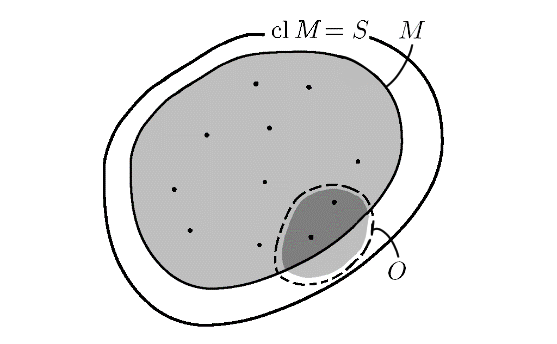
\includegraphics[width=94mm]{8.1.2.a.PNG}
\end{center}
\begin{proof}
位相空間$\left( S,\mathfrak{O} \right)$が与えられたとき、その集合$M$がその集合$S$において稠密であるなら、${\mathrm{cl}}M = S$が成り立つ。したがって、次のようになる。
\begin{align*}
\emptyset = S \setminus S = S \setminus {\mathrm{cl}}M = {\mathrm{int}}(S \setminus M)
\end{align*}
逆に、${\mathrm{int}}(S \setminus M) = \emptyset$が成り立つなら、開核と閉包の関係より${\mathrm{int}}(S \setminus M) = S \setminus {\mathrm{cl}}M$が成り立ち、したがって、${\mathrm{cl}}M = S$が成り立つ。\par
${\mathrm{cl}}M = S$が成り立つかつ、$\exists O \in \mathfrak{O \setminus}\left\{ \emptyset \right\}$に対し、$O \cap M = \emptyset$が成り立つと仮定すると、その集合$O$は空集合ではないので、その集合$M$は空集合であり、空集合は閉集合でもあるので、${\mathrm{cl}}M = {\mathrm{cl}}\emptyset = \emptyset$が成り立つが、これは$S = \emptyset$が成り立つことになり位相の定義に矛盾している。したがって、${\mathrm{cl}}M = S$が成り立つなら、$\forall O \in \mathfrak{O \setminus}\left\{ \emptyset \right\}$に対し、$O \cap M \neq \emptyset$が成り立つ。\par
逆に、${\mathrm{cl}}M \neq S$が成り立つなら、集合$S \setminus {\mathrm{cl}}M$は空集合ではないかつ、開集合となる。したがって、$S \setminus {\mathrm{cl}}M \cap {\mathrm{cl}}M = \emptyset$が成り立つ。ここで、$M \subseteq {\mathrm{cl}}M$が成り立つことに注意すれば、$S \setminus {\mathrm{cl}}M \cap M = \emptyset$も成り立つ。これにより、その集合$M$がその集合$S$において稠密でないなら、$\exists O \in \mathfrak{O \setminus}\left\{ \emptyset \right\}$に対し、$O \cap M = \emptyset$が成り立つことになる。対偶律より、$\forall O \in \mathfrak{O \setminus}\left\{ \emptyset \right\}$に対し、$O \cap M \neq \emptyset$が成り立つなら、その集合$M$はその集合$S$において稠密であることになる。
\end{proof}
\begin{dfn}
位相空間$\left( S,\mathfrak{O} \right)$において、その集合$S$において稠密であるかつ、たかだか可算集合である集合$M$が存在するとき、即ち、$\exists M \in \mathfrak{P}(S)$に対し、${\mathrm{cl}}M = S$が成り立つかつ、${\#}M \leq \aleph_{0}$が成り立つとき、その位相空間$\left( S,\mathfrak{O} \right)$は可分であるなどという。
\end{dfn}
\begin{thm}\label{8.1.2.20}
第2可算公理を満たす位相空間$\left( S,\mathfrak{O} \right)$は可分である。
\end{thm}
\begin{proof}
第2可算公理を満たす位相空間$\left( S,\mathfrak{O} \right)$が与えられたとき、たかだか可算集合であるその位相空間$\left( S,\mathfrak{O} \right)$の開基$\mathfrak{B}$が存在することになる。ここで、その集合$\mathfrak{B}$の元の族$\left\{ W_{\lambda} \right\}_{\lambda \in \varLambda}$が与えられたとき、その添数集合$\varLambda$を空集合とすれば、その和集合$\bigcup_{\lambda \in \varLambda} W_{\lambda}$は空集合となるので、集合$\mathfrak{B \setminus}\left\{ \emptyset \right\}$もその位相空間$\left( S,\mathfrak{O} \right)$の開基となる。ここで、$\forall\lambda \in \varLambda$に対し、選択の公理より$a_{\lambda} \in W_{\lambda}$なる元々$a_{\lambda}$を取り出し次式のように集合$M$が与えられれば、
\begin{align*}
M = \left\{ a_{\lambda} \in S \middle| \forall\lambda \in \varLambda\left[ a_{\lambda} \in W_{\lambda} \right] \right\}
\end{align*}
これはその集合$S$の部分集合となる。ここで、$\forall O \in \mathfrak{O}$に対し、開基の定義より$\exists\lambda \in \varLambda$に対し、$W_{\lambda} \subseteq O$が成り立つので、$a_{\lambda} \in O$が成り立つ。したがって、$a_{\lambda} \in O$かつ$a_{\lambda} \in M$が成り立つので、$O \cap M \neq \emptyset$が成り立つ。これが成り立つならそのときに限り、その集合$M$はその集合$S$において稠密となる。\par
ここで、その開基$\mathfrak{B}$はたかだか可算集合であるので、${\#}\mathfrak{B} \leq \aleph_{0}$が成り立つ。さらに、その集合$\mathfrak{B}$の元の族$\left\{ W_{\lambda} \right\}_{\lambda \in \varLambda}$が与えられているので、${\#}\varLambda \leq {\#}\mathfrak{B}$が成り立つかつ、次式のような写像$f$は明らかに全射であるので、
\begin{align*}
f:\varLambda \rightarrow M;\lambda \mapsto a_{\lambda}
\end{align*}
Bernsteinの定理よりその集合$M$からその集合$\varLambda$への単射が存在し${\#}M \leq {\#}\varLambda$が成り立つ。\par
以上より、${\#}M \leq {\#}\varLambda \leq {\#}\mathfrak{B} \leq \aleph_{0}$が成り立つので、その集合$M$もたかだか可算集合である。これにより、その位相空間$\left( S,\mathfrak{O} \right)$は可分である。
\end{proof}
\begin{thebibliography}{50}
\bibitem{1}
  松坂和夫, 集合・位相入門, 岩波書店, 1968. 新装版第2刷 p165-175 ISBN978-4-00-029871-1
\bibitem{2}
  加塩朋和. "一般位相A(2組)". 東京理科大学. \url{https://www.rs.tus.ac.jp/a25594/2018-2019_General_Topology.pdf} (2021-3-11 取得)
\bibitem{3}
  佃修一. "位相空間問題集". 琉球大学. \url{http://www.math.u-ryukyu.ac.jp/~tsukuda/lecturenotes/exercise-1104.pdf} (2021-3-29 取得)
\end{thebibliography}
\end{document}

\clearpage
\documentclass[dvipdfmx]{jsarticle}
\setcounter{section}{1}
\setcounter{subsection}{2}
\usepackage{xr}
\externaldocument{8.1.1}
\usepackage{amsmath,amsfonts,amssymb,array,comment,mathtools,url,docmute}
\usepackage{longtable,booktabs,dcolumn,tabularx,mathtools,multirow,colortbl,xcolor}
\usepackage[dvipdfmx]{graphics}
\usepackage{bmpsize}
\usepackage{amsthm}
\usepackage{enumitem}
\setlistdepth{20}
\renewlist{itemize}{itemize}{20}
\setlist[itemize]{label=•}
\renewlist{enumerate}{enumerate}{20}
\setlist[enumerate]{label=\arabic*.}
\setcounter{MaxMatrixCols}{20}
\setcounter{tocdepth}{3}
\newcommand{\rotin}{\text{\rotatebox[origin=c]{90}{$\in $}}}
\newcommand{\amap}[6]{\text{\raisebox{-0.7cm}{\begin{tikzpicture} 
  \node (a) at (0, 1) {$\textstyle{#2}$};
  \node (b) at (#6, 1) {$\textstyle{#3}$};
  \node (c) at (0, 0) {$\textstyle{#4}$};
  \node (d) at (#6, 0) {$\textstyle{#5}$};
  \node (x) at (0, 0.5) {$\rotin $};
  \node (x) at (#6, 0.5) {$\rotin $};
  \draw[->] (a) to node[xshift=0pt, yshift=7pt] {$\textstyle{\scriptstyle{#1}}$} (b);
  \draw[|->] (c) to node[xshift=0pt, yshift=7pt] {$\textstyle{\scriptstyle{#1}}$} (d);
\end{tikzpicture}}}}
\newcommand{\twomaps}[9]{\text{\raisebox{-0.7cm}{\begin{tikzpicture} 
  \node (a) at (0, 1) {$\textstyle{#3}$};
  \node (b) at (#9, 1) {$\textstyle{#4}$};
  \node (c) at (#9+#9, 1) {$\textstyle{#5}$};
  \node (d) at (0, 0) {$\textstyle{#6}$};
  \node (e) at (#9, 0) {$\textstyle{#7}$};
  \node (f) at (#9+#9, 0) {$\textstyle{#8}$};
  \node (x) at (0, 0.5) {$\rotin $};
  \node (x) at (#9, 0.5) {$\rotin $};
  \node (x) at (#9+#9, 0.5) {$\rotin $};
  \draw[->] (a) to node[xshift=0pt, yshift=7pt] {$\textstyle{\scriptstyle{#1}}$} (b);
  \draw[|->] (d) to node[xshift=0pt, yshift=7pt] {$\textstyle{\scriptstyle{#2}}$} (e);
  \draw[->] (b) to node[xshift=0pt, yshift=7pt] {$\textstyle{\scriptstyle{#1}}$} (c);
  \draw[|->] (e) to node[xshift=0pt, yshift=7pt] {$\textstyle{\scriptstyle{#2}}$} (f);
\end{tikzpicture}}}}
\renewcommand{\thesection}{第\arabic{section}部}
\renewcommand{\thesubsection}{\arabic{section}.\arabic{subsection}}
\renewcommand{\thesubsubsection}{\arabic{section}.\arabic{subsection}.\arabic{subsubsection}}
\everymath{\displaystyle}
\allowdisplaybreaks[4]
\usepackage{vtable}
\theoremstyle{definition}
\newtheorem{thm}{定理}[subsection]
\newtheorem*{thm*}{定理}
\newtheorem{dfn}{定義}[subsection]
\newtheorem*{dfn*}{定義}
\newtheorem{axs}[dfn]{公理}
\newtheorem*{axs*}{公理}
\renewcommand{\headfont}{\bfseries}
\makeatletter
  \renewcommand{\section}{%
    \@startsection{section}{1}{\z@}%
    {\Cvs}{\Cvs}%
    {\normalfont\huge\headfont\raggedright}}
\makeatother
\makeatletter
  \renewcommand{\subsection}{%
    \@startsection{subsection}{2}{\z@}%
    {0.5\Cvs}{0.5\Cvs}%
    {\normalfont\LARGE\headfont\raggedright}}
\makeatother
\makeatletter
  \renewcommand{\subsubsection}{%
    \@startsection{subsubsection}{3}{\z@}%
    {0.4\Cvs}{0.4\Cvs}%
    {\normalfont\Large\headfont\raggedright}}
\makeatother
\makeatletter
\renewenvironment{proof}[1][\proofname]{\par
  \pushQED{\qed}%
  \normalfont \topsep6\p@\@plus6\p@\relax
  \trivlist
  \item\relax
  {
  #1\@addpunct{.}}\hspace\labelsep\ignorespaces
}{%
  \popQED\endtrivlist\@endpefalse
}
\makeatother
\renewcommand{\proofname}{\textbf{証明}}
\usepackage{tikz,graphics}
\usepackage[dvipdfmx]{hyperref}
\usepackage{pxjahyper}
\hypersetup{
 setpagesize=false,
 bookmarks=true,
 bookmarksdepth=tocdepth,
 bookmarksnumbered=true,
 colorlinks=false,
 pdftitle={},
 pdfsubject={},
 pdfauthor={},
 pdfkeywords={}}
\begin{document}
%\hypertarget{ux9023ux7d9aux5199ux50cf}{%
\subsection{連続写像}%\label{ux9023ux7d9aux5199ux50cf}}
%\hypertarget{ux9023ux7d9aux5199ux50cf-1}{%
\subsubsection{連続写像}%\label{ux9023ux7d9aux5199ux50cf-1}}
\begin{thm}\label{8.1.3.1}
2つの空集合でない集合$S$、$T$における2つのそれぞれの位相たち$\mathfrak{O}$、$\mathfrak{P}$とこれらの閉集合系それぞれ$\mathfrak{A}$、$\mathfrak{B}$、$a \in S$、$b \in T$における全近傍系それぞれ$\mathbf{V}(a)$、$\mathbf{W}(b)$において、写像$f:S \rightarrow T$を考える。このとき、次のことは同値である。
\begin{itemize}
\item
  $\forall P \in \mathfrak{P}$に対し、$V\left( f^{- 1}|P \right) \in \mathfrak{O}$が成り立つ。
\item
  $\forall B \in \mathfrak{B}$に対し、$V\left( f^{- 1}|B \right) \in \mathfrak{A}$が成り立つ。
\item
  $\forall a \in S\forall W \in \mathbf{W}\left( f(a) \right)$に対し、$V\left( f^{- 1}|W \right) \in \mathbf{V}(a)$が成り立つ。
\end{itemize}
\end{thm}
\begin{proof}
2つの空集合でない集合$S$、$T$における2つのそれぞれの位相たち$\mathfrak{O}$、$\mathfrak{P}$とこれらの閉集合系それぞれ$\mathfrak{A}$、$\mathfrak{B}$、$a \in S$、$b \in T$における全近傍系それぞれ$\mathbf{V}(a)$、$\mathbf{W}(b)$において、写像$f:S \rightarrow T$を考える。\par
$\forall P \in \mathfrak{P}$に対し、$V\left( f^{- 1}|P \right)\in \mathfrak{O}$が成り立つなら、$\forall B \in \mathfrak{B}$に対し、$T \setminus B = P$とおけば、定義より明らかに$P \in \mathfrak{P}$が成り立つので、$V\left( f^{- 1}|P \right) \in \mathfrak{P}$が成り立つことと閉集合の定義より次式が成り立つ。
\begin{align*}
V\left( f^{- 1}|B \right) &= V\left( f^{- 1}|T \setminus P \right)\\
&= S \setminus V\left( f^{- 1}|P \right) \in \mathfrak{A}
\end{align*}
逆に、$\forall B \in \mathfrak{B}$に対し、$V\left( f^{- 1}|B \right)\in \mathfrak{A}$が成り立つなら、$\forall P \in \mathfrak{P}$に対し、$T \setminus P = B$とおけば$B \in \mathfrak{B}$が成り立つので、$V\left( f^{- 1}|B \right) \in \mathfrak{B}$より、次式が成り立つ。
\begin{align*}
V\left( f^{- 1}|P \right) &= f^{- 1}(T \setminus B)\\
&= S \setminus V\left( f^{- 1}|B \right) \in \mathfrak{O}
\end{align*}
以上より、次のことは同値である。
\begin{itemize}
\item
  $\forall P \in \mathfrak{P}$に対し、$V\left( f^{- 1}|P \right)\in \mathfrak{O}$が成り立つ。
\item
  $\forall B \in \mathfrak{B}$に対し、$V\left( f^{- 1}|B \right)\in \mathfrak{A}$が成り立つ。
\end{itemize}\par
$\forall P \in \mathfrak{P}$に対し、$V\left( f^{- 1}|P \right)\in \mathfrak{O}$が成り立つなら、$\forall a \in S\forall W \in \mathbf{W}\left( f(a) \right)$に対し、定理\ref{8.1.1.22}より$\exists P \in \mathfrak{P}$に対し、$f(a) \in P \subseteq W$が成り立ち$a \in V\left( f^{- 1}|P \right) \subseteq V\left( f^{- 1}|W \right)$が成り立つ。仮定より$V\left( f^{- 1}|P \right) \in \mathfrak{O}$が成り立ち$a \in V\left( f^{- 1}|P \right) = {\mathrm{int}}{V\left( f^{- 1}|P \right)}$が成り立つので、$V\left( f^{- 1}|P \right) \in \mathbf{W}(a)$が成り立ち、したがって、$V\left( f^{- 1}|W \right) \in \mathbf{V}(a)$が成り立つ。逆に、$\forall a \in S\forall W \in \mathbf{W}\left( f(a) \right)$に対し、$V\left( f^{- 1}|W \right) \in \mathbf{V}(a)$が成り立つなら、$\forall P\in \mathfrak{P}$に対し、$O = V\left( f^{- 1}|P \right)$とすれば、$\forall b \in O$に対し、$f(b) \in V\left( f|V\left( f^{- 1}|P \right) \right) = P$が成り立つかつ、$P \in \mathfrak{P}$より$f(b) \in P = {\mathrm{int}}P$が成り立つので、$P \in \mathbf{V}\left( f(b) \right)$が成り立つ。したがって、仮定より$V\left( f^{- 1}|P \right) = O \in \mathbf{V}(b)$が成り立つ、即ち、$b \in {\mathrm{int}}O$が成り立つので、$O \in \mathfrak{O}$が成り立つ。\par
以上より、次のことは同値である。
\begin{itemize}
\item
  $\forall P \in \mathfrak{P}$に対し、$V\left( f^{- 1}|P \right)\in \mathfrak{O}$が成り立つ。
\item
  $\forall a \in S\forall W \in \mathbf{W}\left( f(a) \right)$に対し、$V\left( f^{- 1}|W \right) \in \mathbf{V}(a)$が成り立つ。
\end{itemize}
\end{proof}
\begin{dfn}
上記のことのいづれかを満たす写像$f:S \rightarrow T$はその定理によって上記の性質たち全て満たすことになり上記の性質たちを満たす写像$f$をその位相空間$\left( S,\mathfrak{O} \right)$からその位相空間$\left( T,\mathfrak{P} \right)$へ連続であるなどといいこのような写像$f$をその位相空間$\left( S,\mathfrak{O} \right)$からその位相空間$\left( T,\mathfrak{P} \right)$への連続写像という。
\end{dfn}\par
例えば、始集合が離散位相$\mathfrak{P}(S)$の台集合である、または、密着位相$\left\{ \emptyset,S \right\}$の台集合であるときは任意の写像$f:S \rightarrow T$は位相的に連続になる。また、2つの空集合でない集合$S$、$T$における2つのそれぞれの位相たち$\mathfrak{O}$、$\mathfrak{P}$においての写像$f:S \rightarrow T$が定値写像であったり、$S = S$かつ$\mathfrak{P} \subseteq \mathfrak{O}$が成り立つときの恒等写像であったりするとき、それらの写像も位相的に連続である。
\begin{thm}\label{8.1.3.2}
2つの位相空間たち$\left( S,\mathfrak{O} \right)$、$\left( T,\mathfrak{P} \right)$が与えられたとする。写像$f:S \rightarrow T$が連続であるならそのときに限り、その位相空間$\left( T,\mathfrak{P} \right)$の準開基$\mathfrak{N}$が与えられたとき、$\forall N \in \mathfrak{N}$に対し、$V\left( f^{- 1}|N \right) \in \mathfrak{O}$が成り立つ。
\end{thm}
\begin{proof}
2つの位相空間たち$\left( S,\mathfrak{O} \right)$、$\left( T,\mathfrak{P} \right)$が与えられたとしその位相空間$\left( T,\mathfrak{P} \right)$の準開基$\mathfrak{N}$が与えられたとき、$\mathfrak{N} \subseteq \mathfrak{P}$が成り立つので、$\forall N \in \mathfrak{N}$に対し、その集合$N$は開集合となる。したがって、写像$f:S \rightarrow T$が連続であるなら、$V\left( f^{- 1}|N \right)\in \mathfrak{O}$が成り立つ。\par
逆に、写像$f:S \rightarrow T$が与えられ、$\forall N\in \mathfrak{N}$に対し、$V\left( f^{- 1}|N \right) \in \mathfrak{O}$が成り立つとき、次式のように集合$\mathfrak{S}$が考えられると、
\begin{align*}
\mathfrak{S} =\left\{ N\in \mathfrak{P}(T) \middle| V\left( f^{- 1}|N \right) \in \mathfrak{O} \right\}
\end{align*}
仮定より、$\forall N\in \mathfrak{N}$に対し、$N\in \mathfrak{S}$が成り立つので、$\mathfrak{N}\subseteq \mathfrak{S}$が成り立つ。また、$V\left( f^{- 1}|T \right) = S$かつ$V\left( f^{- 1}|\emptyset \right) = \emptyset$が明らかに成り立つので、$T,\mathfrak{\emptyset \in S}$が成り立つ。$\forall M,N \in \mathfrak{S}$に対し、次のようになる。
\begin{align*}
M,N \in \mathfrak{S} &\Leftrightarrow V\left( f^{- 1}|M \right),V\left( f^{- 1}|N \right)\in \mathfrak{O}\\
&\Rightarrow V\left( f^{- 1}|M \right) \cap V\left( f^{- 1}|N \right) = V\left( f^{- 1}|M \cap N \right) \in \mathfrak{O}
\end{align*}
これにより、$M \cap N\in \mathfrak{S}$が成り立つ。任意の添数集合$\varLambda$によって添数づけられたその集合$\mathfrak{S}$の元の族$\left\{ M_{\lambda} \right\}_{\scriptsize \begin{matrix}
\lambda \in \varLambda \\
\end{matrix}}$が与えられたとき、次のようになる。
\begin{align*}
\forall\lambda \in \varLambda\left[ M_{\lambda} \in \mathfrak{S} \right] &\Leftrightarrow \forall\lambda \in \varLambda\left[ V\left( f^{- 1} \middle| M_{\lambda} \right) \in \mathfrak{O} \right]\\
&\Rightarrow \bigcup_{\scriptsize \begin{matrix}
\lambda \in \varLambda \\
\end{matrix}} {V\left( f^{- 1} \middle| M_{\lambda} \right)} = V\left( f^{- 1}|\bigcup_{\scriptsize \begin{matrix}
\lambda \in \varLambda \\
\end{matrix}} M_{\lambda} \right) \in \mathfrak{O}
\end{align*}
これにより、$\bigcap_{\scriptsize \begin{matrix}
\lambda \in \varLambda \\
\end{matrix}} M_{\lambda}\in \mathfrak{S}$が成り立つ。以上より、その集合$\mathfrak{S}$は位相である。\par
ここで、その集合$\mathfrak{N}$はその位相空間$\left( T,\mathfrak{P} \right)$の準開基であるので、その集合$\mathfrak{N}$で生成される位相がその位相$\mathfrak{P}$である。したがって、$\mathfrak{N} \subseteq \mathfrak{P}\subseteq \mathfrak{S}$が成り立つので、$\forall P \in \mathfrak{P}$に対し、$V\left( f^{- 1}|P \right) \in \mathfrak{O}$が成り立ちその写像$f$は連続である。
\end{proof}
\begin{dfn}
2つの位相空間たち$\left( S,\mathfrak{O} \right)$、$\left( T,\mathfrak{P} \right)$が与えられたとする。写像$f:S \rightarrow T$において、$a \in S$かつ$b \in T$なる元々$a$、$b$のその位相空間たち$\left( S,\mathfrak{O} \right)$、$\left( T,\mathfrak{P} \right)$の全近傍系たちがそれぞれ$\mathbf{V}(a)$、$\mathbf{W}(b)$とおく。$\forall a \in S\forall W \in \mathbf{W}\left( f(a) \right)$に対し、$V\left( f^{- 1}|W \right) \in \mathbf{V}(a)$が成り立つとき、その写像$f$はその点$a$において連続であるという。
\end{dfn}
\begin{thm}\label{8.1.3.3}
$\forall a \in S$に対し、写像$f:S \rightarrow T$がその点$a$において連続であるならそのときに限り、その写像$f$はその位相空間$\left( S,\mathfrak{O} \right)$からその位相空間$\left( T,\mathfrak{P} \right)$へ連続である。
\end{thm}
\begin{proof}
2つの位相空間たち$\left( S,\mathfrak{O} \right)$、$\left( T,\mathfrak{P} \right)$が与えられたとする。$\forall a \in S$に対し、写像$f:S \rightarrow T$がその点$a$において連続であるならそのときに限り、$a \in S$かつ$b \in T$なる元々$a$、$b$のその位相空間たち$\left( S,\mathfrak{O} \right)$、$\left( T,\mathfrak{P} \right)$の全近傍系たちがそれぞれ$\mathbf{V}(a)$、$\mathbf{W}(b)$とおかれ、$\forall a \in S\forall W \in \mathbf{W}\left( f(a) \right)$に対し、$V\left( f^{- 1}|W \right) \in \mathbf{V}(a)$が成り立つ。これが成り立つならそのときに限り、その写像$f$はその位相空間$\left( S,\mathfrak{O} \right)$からその位相空間$\left( T,\mathfrak{P} \right)$へ連続である。
\end{proof}
\begin{thm}\label{8.1.3.4}
2つの位相空間たち$\left( S,\mathfrak{O} \right)$、$\left( T,\mathfrak{P} \right)$が与えられたとする。写像$f:S \rightarrow T$が$a \in S$なる点$a$において連続であるならそのときに限り、$\forall M \in \mathfrak{P}(S)$に対し、$a \in {\mathrm{cl}}M$が成り立つなら、$f(a) \in {\mathrm{cl}}{V\left( f|M \right)}$も成り立つ。
\end{thm}
\begin{proof}
2つの位相空間たち$\left( S,\mathfrak{O} \right)$、$\left( T,\mathfrak{P} \right)$が与えられたとする。写像$f:S \rightarrow T$が$a \in S$なる点$a$において連続であるとき、$a \in S$かつ$b \in T$なる元々$a$、$b$のその位相空間たち$\left( S,\mathfrak{O} \right)$、$\left( T,\mathfrak{P} \right)$の全近傍系たちがそれぞれ$\mathbf{V}(a)$、$\mathbf{W}(b)$とおかれると、$\forall W \in \mathbf{W}\left( f(a) \right)$に対し、$V\left( f^{- 1}|W \right) \in \mathbf{V}(a)$が成り立つので、$a \in {\mathrm{int}}{V\left( f^{- 1}|W \right)} \subseteq V\left( f^{- 1}|W \right)$が成り立つ。$\forall M \in \mathfrak{P}(S)$に対し、$a \in {\mathrm{cl}}M$が成り立つなら、$V\left( f^{- 1}|W \right) \cap {\mathrm{cl}}M \neq \emptyset$が成り立つことになるので、$V\left( f^{- 1}|W \right) \cap M \neq \emptyset$も成り立つ。また、次のようになり
\begin{align*}
V\left( f|V\left( f^{- 1}|W \right) \cap M \right) &\subseteq V\left( f|V\left( f^{- 1}|W \right) \right) \cap V\left( f|M \right)\\
&\subseteq W \cap V\left( f|M \right)
\end{align*}
その値域$V\left( f|V\left( f^{- 1}|W \right) \cap M \right)$が空集合ではないので、その集合$W \cap V\left( f|M \right)$も空集合ではない。ゆえに、定理\ref{8.1.1.26}より$f(a) \in {\mathrm{cl}}{V\left( f|M \right)}$が成り立つ。\par
逆に、$\forall M \in \mathfrak{P}(S)$に対し、$a \in {\mathrm{cl}}M$が成り立つなら、$f(a) \in {\mathrm{cl}}{V\left( f|M \right)}$も成り立つとき、$\exists W \in \mathbf{W}\left( f(a) \right)$に対し、$V\left( f^{- 1}|W \right) \notin \mathbf{V}(a)$が成り立つと仮定すると、$a \notin {\mathrm{int}}{V\left( f^{- 1}|W \right)}$が成り立つことになるので、次のようになる。
\begin{align*}
a \in S \setminus {\mathrm{int}}{V\left( f^{- 1}|W \right)} &= {\mathrm{cl}}\left( S \setminus V\left( f^{- 1}|W \right) \right)\\
&= {\mathrm{cl}}\left( V\left( f^{- 1} \right) \setminus V\left( f^{- 1}|W \right) \right)\\
&= {\mathrm{cl}}\left( V\left( f^{- 1}|T \right) \setminus V\left( f^{- 1}|W \right) \right)\\
&= {\mathrm{cl}}{V\left( f^{- 1}|T \setminus W \right)}
\end{align*}
したがって、仮定より次のようになる。
\begin{align*}
f(a) \in {\mathrm{cl}}{V\left( f|V\left( f^{- 1}|T \setminus W \right) \right)} &\subseteq {\mathrm{cl}}(T \setminus W)\\
&= T \setminus {\mathrm{int}}W
\end{align*}
これにより、$f(a) \notin {\mathrm{int}}W$が成り立ち、定義より$W \notin \mathbf{W}\left( f(a) \right)$が成り立つことになるが、これは仮定に矛盾する。したがって、$\forall W \in \mathbf{W}\left( f(a) \right)$に対し、$V\left( f^{- 1}|W \right) \in \mathbf{V}(a)$が成り立ち、定義よりその写像$f$はその点$a$において連続である。
\end{proof}
%\hypertarget{ux958bux5199ux50cfux3068ux9589ux5199ux50cf}{%
\subsubsection{開写像と閉写像}%\label{ux958bux5199ux50cfux3068ux9589ux5199ux50cf}}
\begin{dfn}
2つの位相空間たち$\left( S,\mathfrak{O} \right)$、$\left( T,\mathfrak{P} \right)$が与えられたとする。写像$f:S \rightarrow T$において、$\forall O \in \mathfrak{O}$に対し、$V\left( f|O \right) \in \mathfrak{P}$が成り立つ、即ち、その位相$\mathfrak{O}$に属する任意の開集合$O$に制限されたその写像$f$の値域もまたその位相$\mathfrak{P}$に属するとき、その写像$f$は開写像であるという。
\end{dfn}
\begin{dfn}
2つの位相空間たち$\left( S,\mathfrak{O} \right)$、$\left( T,\mathfrak{P} \right)$が与えられたとし写像$f:S \rightarrow T$において、それらの位相たち$\mathfrak{O}$、$\mathfrak{P}$の閉集合系をそれぞれ$\mathfrak{A}$、$\mathfrak{B}$とおくとき、$\forall A \in \mathfrak{A}$に対し、$V\left( f|A \right) \in \mathfrak{B}$が成り立つ、即ち、その閉集合系$\mathfrak{A}$に属する任意の開集合$A$に制限されたその写像$f$の値域もまたその閉集合系$\mathfrak{B}$に属するとき、その写像$f$は閉写像であるという。
\end{dfn}\par
例えば、$\mathfrak{P} = \mathfrak{P}(T)$が成り立つなら、任意の写像$f:S \rightarrow T$は開写像であるかつ、閉写像でもある。$S = T$が成り立つとき、恒等写像$I_{S}:S \rightarrow S$が開写像であるならそのときに限り、$\mathfrak{O} \subseteq \mathfrak{P}$が成り立つ。また、同じくその恒等写像$I_{S}$が閉写像であるならそのときに限り、$\mathfrak{A} \subseteq \mathfrak{B}$が成り立つ。\par
その写像$f$が連続写像であることと、開写像であることと、閉写像であることとは一般に同値ではないことに注意されたい。しかしながら、その写像$f$が全単射であるときでは、連続な写像であることと、開写像であることと、閉写像であることとの間に次に述べる関係がある。
\begin{thm}\label{8.1.3.5}
2つの位相空間たち$\left( S,\mathfrak{O} \right)$、$\left( T,\mathfrak{P} \right)$が与えられたとする。全単射な写像$f:S\overset{\sim}{\rightarrow}T$において、次のことは同値である。
\begin{itemize}
\item
  その写像$f$は開写像である。
\item
  その写像$f$は閉写像である。
\item
  その逆写像$f^{- 1}$は連続写像である。
\end{itemize}
\end{thm}
\begin{proof}
2つの位相空間たち$\left( S,\mathfrak{O} \right)$、$\left( T,\mathfrak{P} \right)$が与えられたとする。それらの位相たち$\mathfrak{O}$、$\mathfrak{P}$の閉集合系をそれぞれ$\mathfrak{A}$、$\mathfrak{B}$とおくとき、全単射な写像$f:S\overset{\sim}{\rightarrow}T$が開写像であるなら、定義より$\forall O \in \mathfrak{O}$に対し、$V\left( f|O \right) \in \mathfrak{P}$が成り立つ。ここで、その写像$f$が単射でもあるので、$V\left( f|S \setminus O \right) = V\left( f|S \right) \setminus V\left( f|O \right)$が成り立つかつ、その写像は全射でもあるので、$V\left( f|S \right) = T$が成り立つことに注意すれば、$\forall A \in \mathfrak{A}$に対し、$A = S \setminus O$なる開集合$O$がその位相$\mathfrak{O}$に存在して次式が成り立つので、
\begin{align*}
V\left( f|A \right) &= V\left( f|S \setminus O \right)\\
&= V\left( f|S \right) \setminus V\left( f|O \right)\\
&= T \setminus V\left( f|O \right) \in \mathfrak{B}
\end{align*}
その写像は閉写像でもある。同様に、その写像が閉写像であるなら、定義より$\forall A \in \mathfrak{A}$に対し、$V\left( f|A \right) \in \mathfrak{B}$が成り立つ。ここで、$\forall O \in \mathfrak{O}$に対し、集合$S \setminus O$が閉集合となり$V\left( f|S \setminus O \right) \in \mathfrak{B}$が成り立ち$V\left( f|S \setminus O \right) = T \setminus P$なる開集合$P$がその位相$\mathfrak{P}$に存在する。その写像$f$が単射でもあるので、$V\left( f|S \setminus (S \setminus O) \right) = V\left( f|S \right) \setminus V\left( f|S \setminus O \right)$が成り立つかつ、その写像は全射でもあるので、$V\left( f|S \right) = T$が成り立つことに注意すれば、次式が成り立つので、
\begin{align*}
V\left( f|O \right) &= V\left( f|S \setminus (S \setminus O) \right)\\
&= V\left( f|S \right) \setminus V\left( f|S \setminus O \right)\\
&= T \setminus V\left( f|S \setminus O \right)\\
&= T \setminus (T \setminus P)\\
&= P \in \mathfrak{P}
\end{align*}
その写像$f$は開写像でもある。以上の議論により、次のことは同値である。
\begin{itemize}
\item
  その写像$f$は開写像である。
\item
  その写像$f$は閉写像である。
\end{itemize}\par
さらに、その写像$f$が開写像であるなら、定義より$\forall O \in \mathfrak{O}$に対し、$V\left( f|O \right) \in \mathfrak{P}$が成り立つことになる。ここで、その写像$f$は全単射なので、これの逆写像$f^{- 1}$が存在し、$f = \left( f^{- 1} \right)^{- 1}$が成り立つので、$V\left( \left( f^{- 1} \right)^{- 1}|O \right) \in \mathfrak{P}$が成り立つ。これにより、その逆写像$f^{- 1}$は連続写像である。逆に、その逆写像$f^{- 1}$が連続写像であるなら、$\forall O \in \mathfrak{O}$に対し、$V\left( \left( f^{- 1} \right)^{- 1}|O \right) \in \mathfrak{P}$が成り立つことになり、$\left( f^{- 1} \right)^{- 1} = f$が成り立つので、$V\left( f|O \right) \in \mathfrak{P}$が成り立つ。これにより、その写像$f$は開写像である。以上の議論により、次のことは同値である。
\begin{itemize}
\item
  その写像$f$は開写像である。
\item
  その逆写像$f^{- 1}$は連続写像である。
\end{itemize}
\end{proof}
\begin{thm}\label{8.1.3.6}
2つの位相空間たち$\left( S,\mathfrak{O} \right)$、$\left( T,\mathfrak{P} \right)$が与えられたとする。$a \in S$かつ$b \in T$なる元々$a$、$b$のその位相空間たち$\left( S,\mathfrak{O} \right)$、$\left( T,\mathfrak{P} \right)$の全近傍系たちがそれぞれ$\mathbf{V}(a)$、$\mathbf{W}(b)$とおかれるとき、写像$f:S \rightarrow T$について、次のことは同値である。
\begin{itemize}
\item
  その写像$f$は開写像である。
\item
  $\forall a \in S\forall V \in \mathbf{V}(a)$に対し、$V\left( f|V \right) \in \mathbf{W}\left( f(a) \right)$が成り立つ。
\item
  その位相空間$\left( S,\mathfrak{O} \right)$の1つの開基$\mathfrak{B}$について、$\forall W \in \mathfrak{B}$に対し、$V\left( f|W \right) \in \mathfrak{P}$が成り立つ。
\end{itemize}
\end{thm}
\begin{proof}
2つの位相空間たち$\left( S,\mathfrak{O} \right)$、$\left( T,\mathfrak{P} \right)$が与えられたとする。$a \in S$かつ$b \in T$なる元々$a$、$b$のその位相空間たち$\left( S,\mathfrak{O} \right)$、$\left( T,\mathfrak{P} \right)$の全近傍系たちがそれぞれ$\mathbf{V}(a)$、$\mathbf{W}(b)$とおかれるとする。写像$f:S \rightarrow T$が開写像であるとき、$\forall a \in S\forall V \in \mathbf{V}(a)$に対し、$a \in {\mathrm{int}}V$が成り立つことになり、したがって、$f(a) \in V\left( f|{\mathrm{int}}V \right)$が成り立つ。ここで、その写像$f$は開写像でその集合${\mathrm{int}}V$はその位相空間$\left( S,\mathfrak{O} \right)$における開集合であるから、その値域$V\left( f|{\mathrm{int}}V \right)$はその位相空間$\left( T,\mathfrak{P} \right)$における開集合となる。したがって、${\mathrm{int}}{V\left( f|{\mathrm{int}}V \right)} = V\left( f|{\mathrm{int}}V \right)$が成り立つ。また、${\mathrm{int}}V \subseteq V$が成り立つので、$V\left( f|{\mathrm{int}}V \right) \subseteq V\left( f|V \right)$が成り立ち、したがって、$V\left( f|{\mathrm{int}}V \right) \subseteq {\mathrm{int}}{V\left( f|V \right)}$が成り立つ。これにより、$f(a) \in {\mathrm{int}}{V\left( f|V \right)}$が成り立ち、定義より$V\left( f|V \right) \in \mathbf{W}\left( f(a) \right)$が得られる。逆に、$\forall a \in S\forall V \in \mathbf{V}(a)$に対し、$V\left( f|V \right) \in \mathbf{W}\left( f(a) \right)$が成り立つなら、$\forall O \in \mathfrak{O}$に対し、$O = \emptyset$のときは明らかなので、空集合でないとすると、$\forall b \in V\left( f|O \right)$に対し、値域の定義より$\exists a \in O$に対し、$f(a) = b$が成り立つことになる。その集合$O$は${\mathrm{int}}O = O$を満たすので、$O \in \mathbf{V}(a)$が成り立ち、$a \in S$が成り立つので、仮定より$V\left( f|O \right) \in \mathbf{W}\left( f(a) \right)$が成り立ち、定義より明らかに、$f(a) = b \in {\mathrm{int}}{V\left( f|O \right)}$が成り立ち、したがって、$V\left( f|O \right) \subseteq {\mathrm{int}}{V\left( f|O \right)}$が成り立つ。${\mathrm{int}}{V\left( f|O \right)} \subseteq V\left( f|O \right)$が成り立つので、${\mathrm{int}}{V\left( f|O \right)} = V\left( f|O \right)$が成り立ちその値域$V\left( f|O \right)$はその位相空間$\left( T,\mathfrak{P} \right)$の開集合となる。これにより、その写像$f$は開写像となる。以上の議論により、次のことは同値である。
\begin{itemize}
\item
  その写像$f$は開写像である。
\item
  $\forall a \in S\forall V \in \mathbf{V}(a)$に対し、$V\left( f|V \right) \in \mathbf{W}\left( f(a) \right)$が成り立つ。
\end{itemize}\par
写像$f:S \rightarrow T$が開写像であるなら、その位相空間$\left( S,\mathfrak{O} \right)$の1つの開基$\mathfrak{B}$について、$\forall W \in \mathfrak{B}$に対し、開基の定義よりその集合$W$はその位相空間$\left( S,\mathfrak{O} \right)$の開集合となりその写像$f$は開写像であるから、定義より明らかに$V\left( f|W \right) \in \mathfrak{P}$が成り立つ。逆に、$\forall W \in \mathfrak{B}$に対し、$V\left( f|W \right) \in \mathfrak{P}$が成り立つなら、開基の定義より$\forall O \in \mathfrak{O}$に対し、添数集合$\varLambda$によって添数づけられたその集合$\mathfrak{B}$の元の族$\left\{ W_{\lambda} \right\}_{\lambda \in \varLambda}$を用いて$O = \bigcup_{\lambda \in \varLambda} W_{\lambda}$が成り立つ。したがって、次のようになり
\begin{align*}
V\left( f|O \right) = V\left( f|\bigcup_{\lambda \in \varLambda} W_{\lambda} \right) = \bigcup_{\lambda \in \varLambda} {V\left( f|W_{\lambda} \right)}
\end{align*}
開基の定義より、$\forall\lambda \in \varLambda$に対し、それらの集合たち$W_{\lambda}$はその位相空間$\left( S,\mathfrak{O} \right)$における開集合たちであるので、仮定より$V\left( f|W_{\lambda} \right) \in \mathfrak{P}$が成り立ち、位相の定義より、$\bigcup_{\lambda \in \varLambda} {V\left( f|W_{\lambda} \right)} \in \mathfrak{P}$が成り立つ。したがって、$V\left( f|O \right) \in \mathfrak{P}$が成り立ちその写像$f$は開写像となる。以上の議論により、次のことは同値である。
\begin{itemize}
\item
  その写像$f$は開写像である。
\item
  $\forall W \in \mathfrak{B}$に対し、$V\left( f|W \right)\in \mathfrak{P}$が成り立つ。
\end{itemize}
\end{proof}
\begin{thm}\label{8.1.3.7}
3つの位相空間たち$\left( S,\mathfrak{O} \right)$、$\left( T,\mathfrak{P} \right)$、$\left( U,\mathfrak{Q} \right)$と写像たち$f:S \rightarrow T$、$g:T \rightarrow U$が与えられたとき、次のことが成り立つ。
\begin{itemize}
\item
  それらの写像たち$f:S \rightarrow T$、$g:S \rightarrow T$がどちらも連続写像であるなら、その合成写像$g \circ f$も連続写像である。
\item
  それらの写像たち$f:S \rightarrow T$、$g:S \rightarrow T$がどちらも開写像であるなら、その合成写像$g \circ f$も開写像である。
\item
  それらの写像たち$f:S \rightarrow T$、$g:S \rightarrow T$がどちらも閉写像であるなら、その合成写像$g \circ f$も閉写像である。
\end{itemize}
\end{thm}
\begin{proof}
3つの位相空間たち$\left( S,\mathfrak{O} \right)$、$\left( T,\mathfrak{P} \right)$、$\left( U,\mathfrak{Q} \right)$と写像たち$f:S \rightarrow T$、$g:T \rightarrow U$が与えられたとする。それらの写像たち$f:S \rightarrow T$、$g:S \rightarrow T$がどちらも連続写像であるなら、定義より$\forall Q \in \mathfrak{Q}$に対し、$V\left( g^{- 1}|Q \right)\in \mathfrak{P}$が成り立ち、さらに、$V\left( f^{- 1}|V\left( g^{- 1}|Q \right) \right) \in \mathfrak{O}$が成り立つ。ここで、値域の定義より$a \in V\left( f^{- 1}|V\left( g^{- 1}|Q \right) \right)$が成り立つならそのときに限り、$\exists b \in V\left( g^{- 1}|Q \right)$に対し、$f(a) = b$が成り立ち、さらに、$\exists c \in Q$に対し、$g(b) = c$が成り立つことになるので、$g\left( f(a) \right) = g \circ f(a) = c$が成り立つ。ゆえに、次式が成り立つ。
\begin{align*}
V\left( f^{- 1}|V\left( g^{- 1}|Q \right) \right) = V\left( (g \circ f)^{- 1}|Q \right) \in \mathfrak{O}
\end{align*}
これにより、その合成写像$g \circ f$は連続写像である。\par
それらの写像たち$f:S \rightarrow T$、$g:S \rightarrow T$がどちらも開写像であるなら、定義より$\forall O \in \mathfrak{O}$に対し、$V\left( f|O \right) \in \mathfrak{P}$が成り立ち、さらに、$V\left( g|V\left( f|O \right) \right) \in \mathfrak{Q}$が成り立つ。ここで、値域の定義より$c \in V\left( g|V\left( f|O \right) \right)$が成り立つならそのときに限り、$\exists b \in V\left( f|O \right)$に対し、$g(b) = c$が成り立ち、さらに、$\exists a \in O$に対し、$f(a) = b$が成り立つことになるので、次式が成り立つ。
\begin{align*}
V\left( g|V\left( f|O \right) \right) = V\left( g \circ f|O \right) \in \mathfrak{Q}
\end{align*}
これにより、その合成写像$g \circ f$は開写像である。\par
それらの写像たち$f:S \rightarrow T$、$g:S \rightarrow T$がどちらも閉写像であるなら、それらの位相空間たち$\left( S,\mathfrak{O} \right)$、$\left( T,\mathfrak{P} \right)$、$\left( U,\mathfrak{Q} \right)$における閉集合系たちをそれぞれ$\mathfrak{A}$、$\mathfrak{B}$、$\mathfrak{C}$とおくと、定義より$\forall A \in \mathfrak{A}$に対し、$V\left( f|A \right) \in \mathfrak{B}$が成り立ち、さらに、$V\left( g|V\left( f|A \right) \right) \in \mathfrak{C}$が成り立つことになる。ここで、上記と同様にして、次式が成り立つことが示される。
\begin{align*}
V\left( g|V\left( f|A \right) \right) = V\left( g \circ f|A \right) \in \mathfrak{C}
\end{align*}
これにより、その合成写像$g \circ f$は閉写像である。
\end{proof}
%\hypertarget{ux540cux76f8ux5199ux50cf}{%
\subsubsection{同相写像}%\label{ux540cux76f8ux5199ux50cf}}
\begin{dfn}
2つの位相空間たち$\left( S,\mathfrak{O} \right)$、$\left( T,\mathfrak{P} \right)$が与えられたとする。写像$f:S \rightarrow T$が全単射であるかつ、連続であるかつ、これの逆写像$f^{- 1}$も連続であるとき、その写像$f$をその位相空間$\left( S,\mathfrak{O} \right)$からその位相空間$\left( T,\mathfrak{P} \right)$への同相写像、位相写像、同位相写像、位相同型写像などという。
\end{dfn}
\begin{thm}\label{8.1.3.8}
3つの位相空間たち$\left( S,\mathfrak{O} \right)$、$\left( T,\mathfrak{P} \right)$、$\left( U,\mathfrak{Q} \right)$と写像たち$f:S \rightarrow T$、$g:T \rightarrow U$が与えられたとき、それらの写像たち$f$、$g$が同相写像であるなら、その合成写像$g \circ f$も同相写像である。
\end{thm}
\begin{proof}
3つの位相空間たち$\left( S,\mathfrak{O} \right)$、$\left( T,\mathfrak{P} \right)$、$\left( U,\mathfrak{Q} \right)$と写像たち$f:S \rightarrow T$、$g:T \rightarrow U$が与えられたとき、それらの写像たち$f$、$g$が同相写像であるなら、これらは全単射でもあるので、もちろん、その合成写像$g \circ f$は全単射である。さらに、それらの写像たち$f$、$g$は連続でもあり定理\ref{8.1.3.7}よりその合成写像$g \circ f$も連続である。ここで、定義よりそれらの逆写像たち$f^{- 1}$、$g^{- 1}$も連続であるので、定理\ref{8.1.3.7}よりその合成写像$f^{- 1} \circ g^{- 1}$も連続である。ここで、$f^{- 1} \circ g^{- 1} = (g \circ f)^{- 1}$が成り立つので、その逆写像$(g \circ f)^{- 1}$も連続である。以上の議論により、その合成写像$g \circ f$も全単射であるかつ、連続であるかつ、開写像であるので、その合成写像$g \circ f$も同相写像である。
\end{proof}
\begin{dfn}
2つの位相空間たち$\left( S,\mathfrak{O} \right)$、$\left( T,\mathfrak{P} \right)$が与えられたとする。これらの間に同相写像が存在するとき、これらは同相である、同位相である、位相同型であるなどといいこのことを$\left( S,\mathfrak{O} \right) \approx \left( T,\mathfrak{P} \right)$などと書きこの関係$\approx$を同相関係という。
\end{dfn}
\begin{thm}\label{8.1.3.9}
同相関係$\approx$は同値関係である、即ち、次のことが成り立つ。
\begin{itemize}
\item
  その関係$\approx$は反射的である、即ち、$\left( S,\mathfrak{O} \right) \approx \left( S,\mathfrak{O} \right)$が成り立つ。
\item
  その関係$\approx$は対称的である、即ち、$\left( S,\mathfrak{O} \right) \approx \left( T,\mathfrak{P} \right)$が成り立つなら、$\left( T,\mathfrak{P} \right) \approx \left( S,\mathfrak{O} \right)$が成り立つ。
\item
  その関係$\approx$は推移的である、即ち、$\left( S,\mathfrak{O} \right) \approx \left( T,\mathfrak{P} \right)$かつ$\left( T,\mathfrak{P} \right) \approx \left( U,\mathfrak{Q} \right)$が成り立つなら、$\left( S,\mathfrak{O} \right) \approx \left( U,\mathfrak{Q} \right)$が成り立つ。
\end{itemize}
\end{thm}
\begin{proof}
1つの位相空間$\left( S,\mathfrak{O} \right)$が与えられたとする。このとき、恒等写像$I_{S}:S \rightarrow S$は明らかに同相写像であるので、$\left( S,\mathfrak{O} \right) \approx \left( S,\mathfrak{O} \right)$が成り立つ。\par
2つの位相空間たち$\left( S,\mathfrak{O} \right)$、$\left( T,\mathfrak{P} \right)$が与えられたとする。$\left( S,\mathfrak{O} \right) \approx \left( T,\mathfrak{P} \right)$が成り立つなら、これらの間に同相写像$f:S \rightarrow T$が存在することになる。ここで、定義よりその写像$f$の逆写像$f^{- 1}:T \rightarrow S$もまた同相写像となるのであったので、$\left( T,\mathfrak{P} \right) \approx \left( S,\mathfrak{O} \right)$が成り立つ。\par
3つの位相空間たち$\left( S,\mathfrak{O} \right)$、$\left( T,\mathfrak{P} \right)$、$\left( U,\mathfrak{Q} \right)$が与えられたとする。$\left( S,\mathfrak{O} \right) \approx \left( T,\mathfrak{P} \right)$かつ$\left( T,\mathfrak{P} \right) \approx \left( U,\mathfrak{Q} \right)$が成り立つなら、同相写像たち$f:S \rightarrow T$、$g:T \rightarrow U$が存在することになる。ここで、定理\ref{8.1.3.8}よりその合成写像$g \circ f:S \rightarrow U$もまた同相写像となるのであったので、$\left( S,\mathfrak{O} \right) \approx \left( U,\mathfrak{Q} \right)$が成り立つ。
\end{proof}
\begin{thm}\label{8.1.3.10}
2つの位相空間たち$\left( S,\mathfrak{O} \right)$、$\left( T,\mathfrak{P} \right)$が与えられたとき、それらの位相空間たち$\left( S,\mathfrak{O} \right)$、$\left( T,\mathfrak{P} \right)$における閉集合系たちをそれぞれ$\mathfrak{A}$、$\mathfrak{B}$、$a \in S$かつ$b \in T$なる元々$a$、$b$のその位相空間たち$\left( S,\mathfrak{O} \right)$、$\left( T,\mathfrak{P} \right)$の全近傍系たちがそれぞれ$\mathbf{V}(a)$、$\mathbf{W}(b)$とおかれると、写像$f:S \rightarrow T$について、次のことは同値である。
\begin{itemize}
\item
  その写像$f$は同相写像である。
\item
  その写像$f$は全単射であるかつ、連続であるかつ、これの逆写像$f^{- 1}$も連続である。
\item
  その写像$f$は全単射であるかつ、連続であるかつ、開写像である。
\item
  その写像$f$は全単射であるかつ、連続であるかつ、閉写像である。
\item
  その逆写像$f^{- 1}$は同相写像である。
\item
  その写像$f$は全単射で、$\forall O \in \mathfrak{O}$に対し、$O \in \mathfrak{O \Leftrightarrow}V\left( f|O \right)\in \mathfrak{P}$が成り立つ。
\item
  その写像$f$は全単射で、$\forall A \in \mathfrak{A}$に対し、$A \in \mathfrak{A \Leftrightarrow}V\left( f|A \right)\in \mathfrak{B}$が成り立つ。
\item
  その写像$f$は全単射で、$\forall a \in S\forall V \in \mathbf{V}(a)$に対し、$V \in \mathbf{V}(a) \Leftrightarrow V\left( f|V \right) \in \mathbf{W}\left( f(a) \right)$が成り立つ。
\item
  その写像$f$は全単射で、$\forall M \in \mathfrak{P}(S)$に対し、$V\left( f|{\mathrm{int}}M \right) = {\mathrm{int}}{V\left( f|M \right)}$が成り立つ。
\item
  その写像$f$は全単射で、$\forall M \in \mathfrak{P}(S)$に対し、$V\left( f|{\mathrm{cl}}M \right) = {\mathrm{cl}}{V\left( f|M \right)}$が成り立つ。
\end{itemize}
\end{thm}
\begin{proof}
2つの位相空間たち$\left( S,\mathfrak{O} \right)$、$\left( T,\mathfrak{P} \right)$が与えられたとき、写像$f:S \rightarrow T$について、それらの位相空間たち$\left( S,\mathfrak{O} \right)$、$\left( T,\mathfrak{P} \right)$における閉集合系たちをそれぞれ$\mathfrak{A}$、$\mathfrak{B}$、$a \in S$かつ$b \in T$なる元々$a$、$b$のその位相空間たち$\left( S,\mathfrak{O} \right)$、$\left( T,\mathfrak{P} \right)$の全近傍系たちがそれぞれ$\mathbf{V}(a)$、$\mathbf{W}(b)$とおかれよう。定義より明らかに次のことは同値である。
\begin{itemize}
\item
  その写像$f$は同相写像である。
\item
  その写像$f$は全単射であるかつ、連続であるかつ、これの逆写像$f^{- 1}$も連続である。
\end{itemize}
定理\ref{8.1.3.5}より明らかに次のことは同値である。
\begin{itemize}
\item
  その写像$f$は全単射であるかつ、連続であるかつ、これの逆写像$f^{- 1}$も連続である。
\item
  その写像$f$は全単射であるかつ、連続であるかつ、開写像である。
\item
  その写像$f$は全単射であるかつ、連続であるかつ、閉写像である。
\end{itemize}
また、その逆写像$f^{- 1}$も全単射で、$\left( f^{- 1} \right)^{- 1} = f$が成り立つことから、次のことは同値である。
\begin{itemize}
\item
  その写像$f$は同相写像である。
\item
  その写像$f$は全単射であるかつ、連続であるかつ、これの逆写像$f^{- 1}$も連続である。
\item
  その逆写像$f^{- 1}$は同相写像である。
\end{itemize}\par
その写像$f$が同相写像であるなら、上記の議論により、その写像$f$は開写像でもあるので、$\forall O \in \mathfrak{O}$に対し、$V\left( f|O \right)\in \mathfrak{P}$が成り立つ。また、上記の議論により、その逆写像$f^{- 1}$も同相写像で開写像でもあり、$V\left( f|O \right)\in \mathfrak{P}$が成り立つなら、$V\left( f^{- 1}|V\left( f|O \right) \right) = O$より$O\in \mathfrak{O}$が成り立つ。これにより、その写像$f$は全単射で$O \in \mathfrak{O \Leftrightarrow}V\left( f|O \right)\in \mathfrak{P}$が成り立つことが示された。逆に、その写像$f$は全単射で、$\forall O \in \mathfrak{O}$に対し、$O \in \mathfrak{O \Leftrightarrow}V\left( f|O \right)\in \mathfrak{P}$が成り立つなら、$\forall P \in \mathfrak{P}$に対し、$O = V\left( f^{- 1}|P \right)$とすれば、その写像$f$は全単射であるので、$P = V\left( f|V\left( f^{- 1}|P \right) \right)$が成り立ち$V\left( f^{- 1}|P \right) \in \mathfrak{O}$が成り立つ。したがって、その写像$f$は連続である。また、その写像$f$は明らかに開写像でもあるので、上記の議論によりしたがって、その写像$f$は同相写像である。以上の議論により、次のことは同値である。
\begin{itemize}
\item
  その写像$f$は同相写像である。
\item
  その写像$f$は全単射で、$\forall O \in \mathfrak{O}$に対し、$O \in \mathfrak{O \Leftrightarrow}V\left( f|O \right)\in \mathfrak{P}$が成り立つ。
\end{itemize}\par
その写像$f$が同相写像であるなら、上記の議論により、その写像$f$は閉写像でもあるので、$\forall A \in \mathfrak{A}$に対し、$V\left( f|A \right) \in \mathfrak{B}$が成り立つ。また、上記の議論により、その逆写像$f^{- 1}$も同相写像で閉写像でもあり、$V\left( f|A \right)\in \mathfrak{B}$が成り立つなら、$V\left( f^{- 1}|V\left( f|A \right) \right) = A$より$A \in \mathfrak{A}$が成り立つ。これにより、その写像$f$は全単射で$A \in \mathfrak{A} \Leftrightarrow V\left( f|A \right) \in \mathfrak{B}$が成り立つことが示された。逆に、その写像$f$は全単射で、$\forall A \in \mathfrak{A}$に対し、$A \in \mathfrak{A} \Leftrightarrow V\left( f|A \right) \in \mathfrak{B}$が成り立つなら、$\forall P \in \mathfrak{P}$に対し、$A = V\left( f^{- 1}|T \setminus P \right)$とすれば、その写像$f$は全単射であるので、$T \setminus P = V\left( f|V\left( f^{- 1}|T \setminus P \right) \right)$が成り立ち$V\left( f^{- 1}|T \setminus P \right) = S \setminus V\left( f^{- 1}|P \right) \in \mathfrak{A}$が成り立つ。したがって、$V\left( f^{- 1}|P \right)\in \mathfrak{O}$が得られその写像$f$は連続である。また、その写像$f$は明らかに閉写像でもあるので、上記の議論によりしたがって、その写像$f$は同相写像である。以上の議論により、次のことは同値である。
\begin{itemize}
\item
  その写像$f$は同相写像である。
\item
  その写像$f$は全単射で、$\forall A \in \mathfrak{A}$に対し、$A \in \mathfrak{A \Leftrightarrow}V\left( f|A \right)\in \mathfrak{B}$が成り立つ。
\end{itemize}\par
写像$f:S \rightarrow T$が同相写像であるなら、定義より明らかにその写像$f$は全単射である。また、その写像$f$の逆写像$f^{- 1}$は連続であるので、$\forall a \in S\forall V \in \mathbf{V}(a)$に対し、$V\left( f|V \right) \in \mathbf{W}\left( f(a) \right)$が成り立つ。また、その写像$f$は連続であるので、$V\left( f|V \right) \in \mathbf{W}\left( f(a) \right)$が成り立つなら、$V\left( f^{- 1}|V\left( f|V \right) \right) \in \mathbf{V}\left( f^{- 1}\left( f(a) \right) \right)$が成り立つ。そこで、その写像$f$は全単射であるので、$V\left( f^{- 1}|V\left( f|V \right) \right) = V$が成り立つかつ、$f^{- 1}\left( f(a) \right) = a$も成り立つので、$V\left( f|V \right) \in \mathbf{W}\left( f(a) \right)$が成り立つなら、$V \in \mathbf{V}(a)$が成り立つ。これにより、その写像$f$は全単射で、$\forall a \in S\forall V \in \mathbf{V}(a)$に対し、$V \in \mathbf{V}(a) \Leftrightarrow V\left( f|V \right) \in \mathbf{W}\left( f(a) \right)$が成り立つことが示された。逆に、その写像$f$は全単射で、$\forall a \in S\forall V \in \mathbf{V}(a)$に対し、$V \in \mathbf{V}(a) \Leftrightarrow V\left( f|V \right) \in \mathbf{W}\left( f(a) \right)$が成り立つなら、$\forall W \in \mathbf{W}\left( f(a) \right)$に対し、その写像$f$が全単射なので、$W = V\left( f|V\left( f^{- 1}|W \right) \right)$が成り立つことにより$V\left( f|V\left( f^{- 1}|W \right) \right) \in \mathbf{W}\left( f(a) \right)$が成り立ち、したがって、$V\left( f^{- 1}|W \right) \in \mathbf{V}(a)$が成り立つ。したがって、その写像$f$は連続である。また、$\forall b \in T$に対し、その写像$f$は全単射なので、$\exists a \in S$に対し、$f(a) = b$が成り立つ。そこで、$\forall V \in \mathbf{V}\left( f^{- 1}(b) \right)$に対し、$V \in \mathbf{V}\left( f^{- 1}(b) \right)$が成り立つなら、$a = f^{- 1}(b)$より$V \in \mathbf{V}(a)$で$V\left( f|V \right) \in \mathbf{W}\left( f(a) \right) = \mathbf{W}(b)$が成り立つ。したがって、その写像$f^{- 1}$は連続である。定義よりしたがって、その写像$f$は同相写像である。以上の議論により、次のことは同値である。
\begin{itemize}
\item
  その写像$f$は同相写像である。
\item
  その写像$f$は全単射で、$\forall a \in S\forall V \in \mathbf{V}(a)$に対し、$V \in \mathbf{V}(a) \Leftrightarrow V\left( f|V \right) \in \mathbf{W}\left( f(a) \right)$が成り立つ。
\end{itemize}\par
その写像$f:S \rightarrow T$が同相写像であるなら、定義より明らかにその写像$f$は全単射である。また、その写像$f$の逆写像$f^{- 1}$が存在し連続であるので、$\forall M\in \mathfrak{P}(S)$に対し、その集合${\mathrm{int}}M$は開集合で$V\left( f|{\mathrm{int}}M \right) \in \mathfrak{P}$が成り立つ。これにより、${\mathrm{int}}M \subseteq M$が成り立つので、$V\left( f|{\mathrm{int}}M \right) \subseteq V\left( f|M \right)$が成り立ち、したがって、$V\left( f|{\mathrm{int}}M \right) \subseteq {\mathrm{int}}{V\left( f|M \right)}$が成り立つ。また、$\exists b \in {\mathrm{int}}{V\left( f|M \right)}$に対し、$b \in {\mathrm{int}}{V\left( f|M \right)}$かつ$b \notin V\left( f|{\mathrm{int}}M \right)$が成り立つと仮定すると、${\mathrm{int}}{V\left( f|M \right)} \subseteq V\left( f|M \right)$が成り立つので、$b \in V\left( f|M \right) \setminus V\left( f|{\mathrm{int}}M \right)$が成り立つ。その写像$f$は全単射なので、次のようになり、
\begin{align*}
b \in V\left( f|M \right) \setminus V\left( f|{\mathrm{int}}M \right) = V\left( f|M \setminus {\mathrm{int}}M \right)
\end{align*}
値域の定義より$\exists a \in M \setminus {\mathrm{int}}M$に対し、$f(a) = b$が成り立ち$a \notin {\mathrm{int}}M$が成り立つ。また、${\mathrm{int}}{V\left( f|M \right)} \in \mathfrak{P}$が成り立ちその写像$f$は連続であるので、$V\left( f^{- 1}|{\mathrm{int}}{V\left( f|M \right)} \right) \in \mathfrak{O}$が成り立つ。したがって、次のようになり
\begin{align*}
V\left( f^{- 1}|{\mathrm{int}}{V\left( f|M \right)} \right) &= {\mathrm{int}}{V\left( f^{- 1}|{\mathrm{int}}{V\left( f|M \right)} \right)}\\
&\subseteq {\mathrm{int}}{V\left( f^{- 1}|V\left( f|M \right) \right)}\\
&= {\mathrm{int}}M
\end{align*}
ここで、$a \notin {\mathrm{int}}M$が成り立つので、$a \notin V\left( f^{- 1}|{\mathrm{int}}{V\left( f|M \right)} \right)$となり、その写像$f$が全単射であることに注意すれば、値域の定義よりしたがって、$f(a) = b \notin {\mathrm{int}}{V\left( f|M \right)}$が成り立つことになるが、これは仮定の$b \in {\mathrm{int}}{V\left( f|M \right)}$が成り立つことに矛盾している。したがって、$\forall b \in {\mathrm{int}}{V\left( f|M \right)}$に対し、$b \in {\mathrm{int}}{V\left( f|M \right)}$が成り立つなら、$b \in V\left( f|{\mathrm{int}}M \right)$が成り立つことになり$V\left( f|{\mathrm{int}}M \right) \supseteq {\mathrm{int}}{V\left( f|M \right)}$が得られる。よって、その写像$f$は全単射で、$\forall M\in \mathfrak{P}(S)$に対し、$V\left( f|{\mathrm{int}}M \right) = {\mathrm{int}}{V\left( f|M \right)}$が成り立つ。逆に、その写像$f:S \rightarrow T$が全単射で、$\forall M\in \mathfrak{P}(S)$に対し、$V\left( f|{\mathrm{int}}M \right) = {\mathrm{int}}{V\left( f|M \right)}$が成り立つなら、$\forall O \in \mathfrak{O}$に対し、次のようになるので、
\begin{align*}
V\left( f|O \right) &= V\left( f|{\mathrm{int}}O \right)\\
&= {\mathrm{int}}{V\left( f|O \right)} \in \mathfrak{P}
\end{align*}
その逆写像$f^{- 1}$は連続である。また、$\forall P \in \mathfrak{P}$に対し、その写像$f$は全単射で次のようになるので、
\begin{align*}
V\left( f^{- 1}|P \right) &= V\left( f^{- 1}|{\mathrm{int}}P \right)\\
&= V\left( f^{- 1}|{\mathrm{int}}{V\left( f|V\left( f^{- 1}|P \right) \right)} \right)\\
&= V\left( f^{- 1}|V\left( f|{\mathrm{int}}{V\left( f^{- 1}|P \right)} \right) \right)\\
&= {\mathrm{int}}{V\left( f^{- 1}|P \right)} \in \mathfrak{O}
\end{align*}
その写像$f$は連続である。よって、その写像$f$は同相写像である。以上の議論により、次のことは同値である。
\begin{itemize}
\item
  その写像$f$は同相写像である。
\item
  その写像$f$は全単射で、$\forall M \in \mathfrak{P}(S)$に対し、$V\left( f|{\mathrm{int}}M \right) = {\mathrm{int}}{V\left( f|M \right)}$が成り立つ。
\end{itemize}\par
その写像$f:S \rightarrow T$が同相写像であるなら、定義より明らかにその写像$f$は全単射である。また、その写像$f$は閉写像でもあるので、$\forall M\in \mathfrak{P}(S)$に対し、その集合${\mathrm{cl}}M$は閉集合で$V\left( f|{\mathrm{cl}}M \right) \in \mathfrak{B}$が成り立つ。これにより、$M \subseteq {\mathrm{cl}}M$が成り立つので、$V\left( f|M \right) \subseteq V\left( f|{\mathrm{cl}}M \right)$が成り立ち、したがって、${\mathrm{cl}}{V\left( f|M \right)} \subseteq V\left( f|{\mathrm{cl}}M \right)$が成り立つ。また、$\exists b \in V\left( f|{\mathrm{cl}}M \right)$に対し、$b \in V\left( f|{\mathrm{cl}}M \right)$かつ$b \notin {\mathrm{cl}}{V\left( f|M \right)}$が成り立つと仮定すると、$V\left( f|M \right) \subseteq {\mathrm{cl}}{V\left( f|M \right)}$が成り立つので、$b \in V\left( f|{\mathrm{cl}}M \right) \setminus V\left( f|M \right)$が成り立つ。その写像$f$は全単射なので、次のようになり、
\begin{align*}
b \in V\left( f|{\mathrm{cl}}M \right) \setminus V\left( f|M \right) = V\left( f|{\mathrm{cl}}M \setminus M \right)
\end{align*}
値域の定義より$\forall a \in {\mathrm{cl}}M \setminus M$に対し、$f(a) = b$が成り立ち$a \in {\mathrm{cl}}M$が成り立つ。また、${\mathrm{cl}}{V\left( f|M \right)} \in \mathfrak{B}$が成り立ちその写像$f$は連続であるので、$V\left( f^{- 1}|{\mathrm{cl}}{V\left( f|M \right)} \right) \in \mathfrak{A}$が成り立つ。したがって、次のようになり
\begin{align*}
{\mathrm{cl}}M &= {\mathrm{cl}}{V\left( f^{- 1}|V\left( f|M \right) \right)}\\
&\subseteq {\mathrm{cl}}{V\left( f^{- 1}|{\mathrm{cl}}{V\left( f|M \right)} \right)}\\
&= V\left( f^{- 1}|{\mathrm{cl}}{V\left( f|M \right)} \right)
\end{align*}
ここで、$a \in {\mathrm{cl}}M$が成り立つので、$a \in V\left( f^{- 1}|{\mathrm{cl}}{V\left( f|M \right)} \right)$となり、その写像$f$が全単射であることに注意すれば、値域の定義よりしたがって、$f(a) = b \in {\mathrm{cl}}{V\left( f|M \right)}$に属することになるが、これは仮定の$b \notin {\mathrm{cl}}{V\left( f|M \right)}$が成り立つことに矛盾している。したがって、$\forall b \in {\mathrm{int}}{V\left( f|M \right)}$に対し、$b \in V\left( f|{\mathrm{cl}}M \right)$が成り立つなら、$b \in {\mathrm{cl}}{V\left( f|M \right)}$が成り立つことになり${\mathrm{cl}}{V\left( f|M \right)} \supseteq V\left( f|{\mathrm{cl}}M \right)$が得られる。よって、その写像$f$は全単射で、$\forall M\in \mathfrak{P}(S)$に対し、${\mathrm{cl}}{V\left( f|M \right)} = V\left( f|{\mathrm{cl}}M \right)$が成り立つ。逆に、その写像$f:S \rightarrow T$が全単射で、$\forall M\in \mathfrak{P}(S)$に対し、${\mathrm{cl}}{V\left( f|M \right)} = V\left( f|{\mathrm{cl}}M \right)$が成り立つなら、$\forall A \in \mathfrak{A}$に対し、次のようになるので、
\begin{align*}
V\left( f|A \right) &= V\left( f|{\mathrm{cl}}A \right)\\
&= {\mathrm{cl}}{V\left( f|A \right)} \in \mathfrak{B}
\end{align*}
その写像$f$は閉写像であり定理\ref{8.1.3.5}よりその逆写像$f^{- 1}$は連続である。また、$\forall B \in \mathfrak{B}$に対し、その写像$f$は全単射で次のようになるので、
\begin{align*}
V\left( f^{- 1}|B \right) &= V\left( f^{- 1}|{\mathrm{cl}}B \right)\\
&= V\left( f^{- 1}|{\mathrm{cl}}{V\left( f|V\left( f^{- 1}|B \right) \right)} \right)\\
&= V\left( f^{- 1}|V\left( f|{\mathrm{cl}}{V\left( f^{- 1}|B \right)} \right) \right)\\
&= {\mathrm{cl}}{V\left( f^{- 1}|B \right)} \in \mathfrak{A}
\end{align*}
その写像$f$は連続である。よって、その写像$f$は同相写像である。以上の議論により、次のことは同値である。
\begin{itemize}
\item
  その写像$f$は同相写像である。
\item
  その写像$f$は全単射で、$\forall M \in \mathfrak{P}(S)$に対し、$V\left( f|{\mathrm{cl}}M \right) = {\mathrm{cl}}{V\left( f|M \right)}$が成り立つ。
\end{itemize}
\end{proof}
\begin{thebibliography}{50}
\bibitem{1}
  松坂和夫, 集合・位相入門, 岩波書店, 1968. 新装版第2刷 p175-186 ISBN978-4-00-029871-1
\end{thebibliography}
\end{document}

\clearpage
\documentclass[dvipdfmx]{jsarticle}
\setcounter{section}{1}
\setcounter{subsection}{3}
\usepackage{xr}
\externaldocument{8.1.1}
\usepackage{amsmath,amsfonts,amssymb,array,comment,mathtools,url,docmute}
\usepackage{longtable,booktabs,dcolumn,tabularx,mathtools,multirow,colortbl,xcolor}
\usepackage[dvipdfmx]{graphics}
\usepackage{bmpsize}
\usepackage{amsthm}
\usepackage{enumitem}
\setlistdepth{20}
\renewlist{itemize}{itemize}{20}
\setlist[itemize]{label=•}
\renewlist{enumerate}{enumerate}{20}
\setlist[enumerate]{label=\arabic*.}
\setcounter{MaxMatrixCols}{20}
\setcounter{tocdepth}{3}
\newcommand{\rotin}{\text{\rotatebox[origin=c]{90}{$\in $}}}
\newcommand{\amap}[6]{\text{\raisebox{-0.7cm}{\begin{tikzpicture} 
  \node (a) at (0, 1) {$\textstyle{#2}$};
  \node (b) at (#6, 1) {$\textstyle{#3}$};
  \node (c) at (0, 0) {$\textstyle{#4}$};
  \node (d) at (#6, 0) {$\textstyle{#5}$};
  \node (x) at (0, 0.5) {$\rotin $};
  \node (x) at (#6, 0.5) {$\rotin $};
  \draw[->] (a) to node[xshift=0pt, yshift=7pt] {$\textstyle{\scriptstyle{#1}}$} (b);
  \draw[|->] (c) to node[xshift=0pt, yshift=7pt] {$\textstyle{\scriptstyle{#1}}$} (d);
\end{tikzpicture}}}}
\newcommand{\twomaps}[9]{\text{\raisebox{-0.7cm}{\begin{tikzpicture} 
  \node (a) at (0, 1) {$\textstyle{#3}$};
  \node (b) at (#9, 1) {$\textstyle{#4}$};
  \node (c) at (#9+#9, 1) {$\textstyle{#5}$};
  \node (d) at (0, 0) {$\textstyle{#6}$};
  \node (e) at (#9, 0) {$\textstyle{#7}$};
  \node (f) at (#9+#9, 0) {$\textstyle{#8}$};
  \node (x) at (0, 0.5) {$\rotin $};
  \node (x) at (#9, 0.5) {$\rotin $};
  \node (x) at (#9+#9, 0.5) {$\rotin $};
  \draw[->] (a) to node[xshift=0pt, yshift=7pt] {$\textstyle{\scriptstyle{#1}}$} (b);
  \draw[|->] (d) to node[xshift=0pt, yshift=7pt] {$\textstyle{\scriptstyle{#2}}$} (e);
  \draw[->] (b) to node[xshift=0pt, yshift=7pt] {$\textstyle{\scriptstyle{#1}}$} (c);
  \draw[|->] (e) to node[xshift=0pt, yshift=7pt] {$\textstyle{\scriptstyle{#2}}$} (f);
\end{tikzpicture}}}}
\renewcommand{\thesection}{第\arabic{section}部}
\renewcommand{\thesubsection}{\arabic{section}.\arabic{subsection}}
\renewcommand{\thesubsubsection}{\arabic{section}.\arabic{subsection}.\arabic{subsubsection}}
\everymath{\displaystyle}
\allowdisplaybreaks[4]
\usepackage{vtable}
\theoremstyle{definition}
\newtheorem{thm}{定理}[subsection]
\newtheorem*{thm*}{定理}
\newtheorem{dfn}{定義}[subsection]
\newtheorem*{dfn*}{定義}
\newtheorem{axs}[dfn]{公理}
\newtheorem*{axs*}{公理}
\renewcommand{\headfont}{\bfseries}
\makeatletter
  \renewcommand{\section}{%
    \@startsection{section}{1}{\z@}%
    {\Cvs}{\Cvs}%
    {\normalfont\huge\headfont\raggedright}}
\makeatother
\makeatletter
  \renewcommand{\subsection}{%
    \@startsection{subsection}{2}{\z@}%
    {0.5\Cvs}{0.5\Cvs}%
    {\normalfont\LARGE\headfont\raggedright}}
\makeatother
\makeatletter
  \renewcommand{\subsubsection}{%
    \@startsection{subsubsection}{3}{\z@}%
    {0.4\Cvs}{0.4\Cvs}%
    {\normalfont\Large\headfont\raggedright}}
\makeatother
\makeatletter
\renewenvironment{proof}[1][\proofname]{\par
  \pushQED{\qed}%
  \normalfont \topsep6\p@\@plus6\p@\relax
  \trivlist
  \item\relax
  {
  #1\@addpunct{.}}\hspace\labelsep\ignorespaces
}{%
  \popQED\endtrivlist\@endpefalse
}
\makeatother
\renewcommand{\proofname}{\textbf{証明}}
\usepackage{tikz,graphics}
\usepackage[dvipdfmx]{hyperref}
\usepackage{pxjahyper}
\hypersetup{
 setpagesize=false,
 bookmarks=true,
 bookmarksdepth=tocdepth,
 bookmarksnumbered=true,
 colorlinks=false,
 pdftitle={},
 pdfsubject={},
 pdfauthor={},
 pdfkeywords={}}
\begin{document}
%\hypertarget{ux8a98ux5c0eux4f4dux76f8ux7a7aux9593}{%
\subsection{誘導位相空間}%\label{ux8a98ux5c0eux4f4dux76f8ux7a7aux9593}}
%\hypertarget{ux8a98ux5c0eux4f4dux76f8ux7a7aux9593-1}{%
\subsubsection{誘導位相空間}%\label{ux8a98ux5c0eux4f4dux76f8ux7a7aux9593-1}}\par
1つの集合$S$と1つの位相空間$\left( T,\mathfrak{P} \right)$、1つの写像$f:S \rightarrow T$が与えられたとき、その写像$f$がある位相空間$\left( S,\mathfrak{O} \right)$からその位相空間$\left( T,\mathfrak{P} \right)$への連続写像となるようなその位相$\mathfrak{O}$を求めたい。しかしながら、このような位相$\mathfrak{O}$が存在したとすれば、これより強い位相$\mathfrak{O}'$を用いて$\forall P \in \mathfrak{P}$に対し、$V\left( f^{- 1}|P \right)\in \mathfrak{O \subseteq}\mathfrak{O}'$が成り立ちその写像$f$はその位相空間$\left( S,\mathfrak{O}' \right)$からその位相空間$\left( T,\mathfrak{P} \right)$への連続写像となるので、その位相$\mathfrak{O}$は必ずしも一意的に決まるとは限らない。
\begin{thm}\label{8.1.4.1}
1つの集合$S$と1つの位相空間$\left( T,\mathfrak{P} \right)$、1つの写像$f:S \rightarrow T$が与えられたとき、その写像$f$がある位相空間$\left( S,\mathfrak{O} \right)$からその位相空間$\left( T,\mathfrak{P} \right)$への連続写像となるような位相たち$\mathfrak{O}$のうち、最も強いものは離散位相$\mathfrak{P}(S)$である。
\end{thm}
\begin{proof}
1つの集合$S$と1つの位相空間$\left( T,\mathfrak{P} \right)$、1つの写像$f:S \rightarrow T$が与えられたとき、その集合$S$を台集合とする離散位相$\mathfrak{P}(S)$について、$\forall P \in \mathfrak{P}$に対し、値域の定義より$V\left( f^{- 1}|P \right)\in \mathfrak{P}(S)$が必ず成り立つ。さらに、その離散位相$\mathfrak{P}(S)$はその集合$S$を台集合とするその写像$f$がある位相空間$\left( S,\mathfrak{O} \right)$からその位相空間$\left( T,\mathfrak{P} \right)$への連続写像となるような任意の位相$\mathfrak{O}$に対し、$\mathfrak{O \subseteq P}(S)$を満たすので、このような位相たち$\mathfrak{O}$のうち、最も強いものはその離散位相$\mathfrak{P}(S)$となる。
\end{proof}
\begin{thm}\label{8.1.4.2}
1つの集合$S$と1つの位相空間$\left( T,\mathfrak{P} \right)$、1つの写像$f:S \rightarrow T$が与えられたとき、その写像$f$がある位相空間$\left( S,\mathfrak{O} \right)$からその位相空間$\left( T,\mathfrak{P} \right)$への連続写像となるような位相たち$\mathfrak{O}$のうち、最も弱いものは次式のように定義されるその位相$\mathfrak{P}$の元$P$のその逆対応$f^{- 1}$による値域$V\left( f^{- 1}|P \right)$全体の集合$\mathfrak{O}_{0}$である。
\begin{align*}
\mathfrak{O}_{0} = \left\{ O'\in \mathfrak{P}(S) \middle| \exists P \in \mathfrak{P}\left[ O' = V\left( f^{- 1}|P \right) \right] \right\}
\end{align*}
\end{thm}
\begin{dfn}
この位相$\mathfrak{O}_{0}$をその写像$f$によってその位相空間$\left( T,\mathfrak{P} \right)$から誘導される位相、その写像$f$によるその位相空間$\left( T,\mathfrak{P} \right)$からの誘導位相、始位相などといいその位相空間$\left( S,\mathfrak{O}_{0} \right)$をその写像$f$によるその位相空間$\left( T,\mathfrak{P} \right)$からの誘導位相空間、始位相空間などという。
\end{dfn}
\begin{proof}
1つの集合$S$と1つの位相空間$\left( T,\mathfrak{P} \right)$、1つの写像$f:S \rightarrow T$が与えられたとし、次式のようにその位相$\mathfrak{P}$の元$P$のその逆対応$f^{- 1}$による値域$V\left( f^{- 1}|P \right)$全体の集合$\mathfrak{O}_{0}$が定義される。
\begin{align*}
\mathfrak{O}_{0} = \left\{ O'\in \mathfrak{P}(S) \middle| \exists P \in \mathfrak{P}\left[ O' = V\left( f^{- 1}|P \right) \right] \right\}
\end{align*}
このとき、位相の定義より$T \in \mathfrak{P}$が成り立つかつ、$D(f) = V\left( f^{- 1} \right)$が成り立つかつ、その対応$f$が写像であるので、$D(f) = S$が成り立つことに注意すれば、$V\left( f^{- 1}|T \right) = S$が成り立つ。さらに、位相の定義より$\mathfrak{\emptyset \in P}$が成り立つので、$V\left( f^{- 1}|\emptyset \right) = \emptyset$が成り立つ。以上より、$S,\emptyset \in \mathfrak{O}_{0}$が成り立つ。任意の添数集合$\varLambda$によって添数づけられたその集合$\mathfrak{O}_{0}$の元の族$\left\{ O_{\lambda} \right\}_{\lambda \in \varLambda}$が与えられたとき、その集合$\mathfrak{O}_{0}$の定義より$\forall\lambda \in \varLambda\exists P_{\lambda}\in \mathfrak{P}$に対し、$O_{\lambda} = V\left( f^{- 1}|P_{\lambda} \right)$が成り立つ。ここで、位相の定義より$\bigcup_{\lambda \in \varLambda} P_{\lambda}\in \mathfrak{P}$が成り立つかつ、次式が成り立つ。
\begin{align*}
V\left( f^{- 1}|\bigcup_{\lambda \in \varLambda} P_{\lambda} \right) &= \bigcup_{\lambda \in \varLambda} {V\left( f^{- 1}|P_{\lambda} \right)}\\
&= \bigcup_{\lambda \in \varLambda} O_{\lambda} \in \mathfrak{O}_{0}
\end{align*}
$\forall O,P \in \mathfrak{O}_{0}$に対し、その集合$\mathfrak{O}_{0}$の定義より$\exists Q,R \in \mathfrak{P}$に対し、$O = V\left( f^{- 1}|Q \right)$かつ$P = V\left( f^{- 1}|R \right)$が成り立つ。ここで、位相の定義より$Q \cap R \in \mathfrak{P}$が成り立つかつ、その対応$f$は写像であり次式が成り立つ。
\begin{align*}
V\left( f^{- 1}|Q \cap R \right) &= V\left( f^{- 1}|Q \right) \cap V\left( f^{- 1}|R \right)\\
&= O \cap P \in \mathfrak{O}_{0}
\end{align*}
以上より、その集合$\mathfrak{O}_{0}$はその集合$S$を台集合とする位相である。また、その位相$\mathfrak{O}_{0}$の定義より$\forall P \in \mathfrak{P}$に対し、$V\left( f^{- 1}|P \right) \in \mathfrak{O}_{0}$が成り立つので、その写像$f$は連続写像である。\par
さらに、その写像$f$がある位相空間$\left( S,\mathfrak{O} \right)$からその位相空間$\left( T,\mathfrak{P} \right)$への連続写像となるとき、$\forall O \in \mathfrak{O}_{0}\exists P \in \mathfrak{P}$に対し、$O = V\left( f^{- 1}|P \right)$が成り立つので、$O = V\left( f^{- 1}|P \right)\in \mathfrak{O}$が成り立つ。したがって、このような位相$\mathfrak{O}$すべて$\mathfrak{O}_{0}\subseteq \mathfrak{O}$を満たす。\par
以上より、このような位相たち$\mathfrak{O}$のうち、最も弱いものはその位相$\mathfrak{O}_{0}$となる。
\end{proof}\par
さらに、1つの集合$S$と添数集合$\varLambda$によって添数づけられた位相空間の族$\left\{ \left( S_{\lambda},\mathfrak{O}_{\lambda} \right) \right\}_{\lambda \in \varLambda}$、その添数集合$\varLambda$によって添数づけられた写像の族$\left\{ f_{\lambda}:S \rightarrow S_{\lambda} \right\}_{\lambda \in \varLambda}$が与えられたとき、$\forall\lambda \in \varLambda$に対し、それらの写像たち$f_{\lambda}$がある位相空間$\left( S,\mathfrak{O} \right)$からその位相空間$\left( S_{\lambda},\mathfrak{O}_{\lambda} \right)$への連続写像となるようなその位相$\mathfrak{O}$を求めたい。
\begin{thm}\label{8.1.4.3}
このような位相$\mathfrak{O}$のうち最も強いものはやはり離散位相$\mathfrak{P}\left( \mathfrak{O} \right)$となる。
\end{thm}
\begin{proof}
1つの集合$S$と添数集合$\varLambda$によって添数づけられた位相空間の族$\left\{ \left( S_{\lambda},\mathfrak{O}_{\lambda} \right) \right\}_{\lambda \in \varLambda}$、その添数集合$\varLambda$によって添数づけられた写像の族$\left\{ f_{\lambda}:S \rightarrow S_{\lambda} \right\}_{\lambda \in \varLambda}$が与えられたとき、その集合$S$を台集合とする離散位相$\mathfrak{P}(S)$について、$\forall\lambda \in \varLambda\forall O_{\lambda} \in \mathfrak{O}_{\lambda}$に対し、値域の定義より$V\left( f^{- 1}|O_{\lambda} \right)\in \mathfrak{P}(S)$が必ず成り立つ。さらに、その離散位相$\mathfrak{P}(S)$はその集合$S$を台集合とする任意の位相たち$\mathfrak{O}$を用いて$\mathfrak{O \subseteq P}(S)$を満たすので、$\forall\lambda \in \varLambda$に対し、それらの写像たち$f_{\lambda}$がある位相空間$\left( S,\mathfrak{O} \right)$からその位相空間$\left( S_{\lambda},\mathfrak{O}_{\lambda} \right)$への連続写像となるような位相たち$\mathfrak{O}$のうち、最も強いものはその離散位相$\mathfrak{P}(S)$となる。
\end{proof}
\begin{thm}\label{8.1.4.4}
このような位相$\mathfrak{O}$のうち最も弱いのは次式のように定義されるその集合$S$を台集合とする位相全体の集合$\mathcal{T}(S)$を用いた順序集合$\left( \mathcal{T}(S), \subseteq \right)$におけるその写像$f_{\lambda}$によるその位相空間$\left( S_{\lambda},\mathfrak{O}_{\lambda} \right)$からの誘導位相$\mathfrak{O}_{\lambda}'$全体の集合の上限$\mathfrak{O}_{0}$である。
\begin{align*}
\mathfrak{O}_{0} = \sup\left\{ \mathfrak{O}_{\lambda}'\in \mathcal{T}(S) \middle| \lambda \in \varLambda \right\}
\end{align*}
\end{thm}
\begin{dfn}
この位相$\mathfrak{O}_{0}$をその写像の族$\left\{ f_{\lambda}:S \rightarrow S_{\lambda} \right\}_{\lambda \in \varLambda}$によってその位相空間の族$\left\{ \left( S_{\lambda},\mathfrak{O}_{\lambda} \right) \right\}_{\lambda \in \varLambda}$から誘導される位相、その写像の族$\left\{ f_{\lambda}:S \rightarrow S_{\lambda} \right\}_{\lambda \in \varLambda}$によるその位相空間の族$\left\{ \left( S_{\lambda},\mathfrak{O}_{\lambda} \right) \right\}_{\lambda \in \varLambda}$からの誘導位相、始位相などといいその位相空間$\left( S,\mathfrak{O}_{0} \right)$をその写像の族$\left\{ f_{\lambda}:S \rightarrow S_{\lambda} \right\}_{\lambda \in \varLambda}$によるその位相空間の族$\left\{ \left( S_{\lambda},\mathfrak{O}_{\lambda} \right) \right\}_{\lambda \in \varLambda}$からの誘導位相空間、始位相空間などという。
\end{dfn}
\begin{proof}
1つの集合$S$と添数集合$\varLambda$によって添数づけられた位相空間の族$\left\{ \left( S_{\lambda},\mathfrak{O}_{\lambda} \right) \right\}_{\lambda \in \varLambda}$、その添数集合$\varLambda$によって添数づけられた写像の族$\left\{ f_{\lambda}:S \rightarrow S_{\lambda} \right\}_{\lambda \in \varLambda}$が与えられたとき、$\forall\lambda \in \varLambda$に対し、その写像$f_{\lambda}$によるその位相空間$\left( S_{\lambda},\mathfrak{O}_{\lambda} \right)$からの誘導位相を$\mathfrak{O}_{\lambda}'$とおくと、それらの写像たち$f_{\lambda}$がその位相空間$\left( S,\mathfrak{O}_{\lambda}' \right)$からその位相空間$\left( S_{\lambda},\mathfrak{O}_{\lambda} \right)$への連続写像となり、$\forall\lambda \in \varLambda\forall O_{\lambda} \in \mathfrak{O}_{\lambda}$に対し、$V\left( f^{- 1}|O_{\lambda} \right) \in \mathfrak{O}_{\lambda}'$が成り立つ。その集合$S$を台集合とする位相全体の集合$\mathcal{T}$を用いた順序集合$\left( \mathcal{T}(S), \subseteq \right)$を考え、それらの誘導位相$\mathfrak{O}_{\lambda}'$全体の集合$\left\{ \mathfrak{O}_{\lambda}'\in \mathcal{T}(S) \middle| \lambda \in \varLambda \right\}$の任意の上界$\mathfrak{O}'$、即ち、$\forall\lambda \in \varLambda$に対し、$\mathfrak{O}_{\lambda}' \subseteq \mathfrak{O}'$が成り立つような任意の位相$\mathfrak{O}'$は、$\forall\lambda \in \varLambda\forall O_{\lambda} \in \mathfrak{O}_{\lambda}$に対し、$V\left( f^{- 1}|O_{\lambda} \right) \in \mathfrak{O}'$を満たすので、その位相$\mathfrak{O}'$は、$\forall\lambda \in \varLambda$に対し、それらの写像たち$f_{\lambda}$がある位相空間$\left( S,\mathfrak{O} \right)$からその位相空間$\left( S_{\lambda},\mathfrak{O}_{\lambda} \right)$への連続写像となる。ここで、それらの誘導位相$\mathfrak{O}_{\lambda}'$全体の集合$\left\{ \mathfrak{O}_{\lambda}'\in \mathcal{T}(S) \middle| \lambda \in \varLambda \right\}$はその集合$\mathcal{T}(S)$の元の族でありこの集合$\left\{ \mathfrak{O}_{\lambda}'\in \mathcal{T}(S) \middle| \lambda \in \varLambda \right\}$の上限がその集合$\mathcal{T}(S)$に存在するのであったので、$\forall\lambda \in \varLambda$に対し、それらの写像たち$f_{\lambda}$がある位相空間$\left( S,\mathfrak{O} \right)$からその位相空間$\left( S_{\lambda},\mathfrak{O}_{\lambda} \right)$への連続写像となるような位相$\mathfrak{O}'$全体の集合のうち最も弱いものがその順序集合$\left( \mathcal{T, \subseteq} \right)$における上限$\sup\left\{ \mathfrak{O}_{\lambda}'\in \mathcal{T}(S) \middle| \lambda \in \varLambda \right\}$となる。
\end{proof}
\begin{thm}\label{8.1.4.5}
写像の族$\left\{ f_{\lambda}:S \rightarrow S_{\lambda} \right\}_{\lambda \in \varLambda}$によるその位相空間の族$\left\{ \left( S_{\lambda},\mathfrak{O}_{\lambda} \right) \right\}_{\lambda \in \varLambda}$からの誘導位相$\mathfrak{O}_{0}$は次式を満たす、即ち、その和集合$\bigcup_{\lambda \in \varLambda} \mathfrak{O}_{\lambda}$で生成される位相$\mathfrak{O}\left( \bigcup_{\lambda \in \varLambda} \mathfrak{O}_{\lambda}' \right)$に等しい。
\begin{align*}
\mathfrak{O}_{0} = \mathfrak{O}\left( \bigcup_{\lambda \in \varLambda} \mathfrak{O}_{\lambda}' \right)
\end{align*}
さらに、集合$\mathfrak{B}$が次式のように定義されると、
\begin{align*}
\mathfrak{B} = \left\{ \bigcap_{\scriptsize \begin{matrix}
\mu \in M \\
\end{matrix}} A_{\mu}\in \mathfrak{P}(S) \middle| {\#}M < \aleph_{0},\ \ \forall\mu \in M\left[ A_{\mu} \in \bigcup_{\lambda \in \varLambda} \mathfrak{O}_{\lambda}' \right] \right\}
\end{align*}
次式が成り立つ、
\begin{align*}
\mathfrak{O}_{0} = \left\{ \bigcup_{\nu \in N} B_{\nu}\in \mathfrak{P}(S) \middle| \forall\nu \in N\left[ B_{\nu}\in \mathfrak{B} \right] \right\}
\end{align*}
即ち、その誘導位相$\mathfrak{O}_{0}$はその和集合$\bigcup_{\lambda \in \varLambda} \mathfrak{O}_{\lambda}$を用いて$A_{\mu} \in \bigcup_{\lambda \in \varLambda} \mathfrak{O}_{\lambda}$なる有限個の集合たち$A_{\mu}$の共通部分$\bigcap_{\scriptsize \begin{matrix}
\mu \in M \\
\end{matrix}} A_{\mu}$全体の集合$\mathfrak{B}$を用いて$B_{\nu} \in \mathfrak{B}$なる集合$B_{\nu}$の和集合$\bigcup_{\nu \in N} B_{\nu}$で表される集合全体の集合である。
\end{thm}
\begin{proof}
1つの集合$S$と添数集合$\varLambda$によって添数づけられた位相空間の族$\left\{ \left( S_{\lambda},\mathfrak{O}_{\lambda} \right) \right\}_{\lambda \in \varLambda}$、その添数集合$\varLambda$によって添数づけられた写像の族$\left\{ f_{\lambda}:S \rightarrow S_{\lambda} \right\}_{\lambda \in \varLambda}$が与えられたとき、写像の族$\left\{ f_{\lambda}:S \rightarrow S_{\lambda} \right\}_{\lambda \in \varLambda}$によるその位相空間の族$\left\{ \left( S_{\lambda},\mathfrak{O}_{\lambda} \right) \right\}_{\lambda \in \varLambda}$からの誘導位相$\mathfrak{O}_{0}$は次式のようにその集合$S$を台集合とする位相全体の集合$\mathcal{T}(S)$を用いた順序集合$\left( \mathcal{T}(S), \subseteq \right)$におけるその写像$f_{\lambda}$によるその位相空間$\left( S_{\lambda},\mathfrak{O}_{\lambda} \right)$からの誘導位相$\mathfrak{O}_{\lambda}'$全体の集合の上限$\mathfrak{O}_{0}$であるのであった。
\begin{align*}
\mathfrak{O}_{0} = \sup\left\{ \mathfrak{O}_{\lambda}'\in \mathcal{T}(S) \middle| \lambda \in \varLambda \right\}
\end{align*}
ここで、$\forall\lambda \in \varLambda$に対し、$\mathfrak{O}_{\lambda}' \subseteq \bigcup_{\lambda \in \varLambda} \mathfrak{O}_{\lambda}'$が成り立ち、$\forall\lambda \in \varLambda$に対し、$\mathfrak{O}_{\lambda}' \subseteq \mathfrak{O}'$が成り立つならそのときに限り、$\bigcup_{\lambda \in \varLambda} \mathfrak{O}_{\lambda}' \subseteq \mathfrak{O}'$が成り立つので、集合$\mathfrak{O}'$がその集合$\left\{ \mathfrak{O}_{\lambda}'\in \mathcal{T}(S) \middle| \lambda \in \varLambda \right\}$の上界であるならそのときに限り、$\bigcup_{\lambda \in \varLambda} \mathfrak{O}_{\lambda}' \subseteq \mathfrak{O}'$が成り立つことになる。したがって、その集合$\left\{ \mathfrak{O}_{\lambda}'\in \mathcal{T}(S) \middle| \lambda \in \varLambda \right\}$の上限$\sup\left\{ \mathfrak{O}_{\lambda}'\in \mathcal{T} \middle| \lambda \in \varLambda \right\}$は$\bigcup_{\lambda \in \varLambda} \mathfrak{O}_{\lambda}' \subseteq \mathfrak{O}'$が成り立つような位相$\mathfrak{O}'$のうち最も弱いので、定義より$\mathfrak{O}_{0} = \mathfrak{O}\left( \bigcup_{\lambda \in \varLambda} \mathfrak{O}_{\lambda}' \right)$のようにその位相$\mathfrak{O}_{0}$はその集合$\bigcup_{\lambda \in \varLambda} \mathfrak{O}_{\lambda}'$で生成される位相$\mathfrak{O}\left( \bigcup_{\lambda \in \varLambda} \mathfrak{O}_{\lambda}' \right)$である。\par
このとき、その位相$\mathfrak{O}_{0}$は、有限集合である添数集合$M$によって添数づけられたその集合$\bigcup_{\lambda \in \varLambda} \mathfrak{O}_{\lambda}'$の元の族$\left\{ A_{\mu} \right\}_{\mu \in M}$の積集合全体の集合を$\mathfrak{B}$として、任意の添数集合$N$によって添数づけられたその集合$\mathfrak{B}$の元の族$\left\{ B_{\nu} \right\}_{\nu \in N}$の和集合全体の集合に等しいのであったので、集合$\mathfrak{B}$が次式のように定義されると、
\begin{align*}
\mathfrak{B} =\left\{ \bigcap_{\scriptsize \begin{matrix}
\mu \in M \\
\end{matrix}} A_{\mu}\in \mathfrak{P}(S) \middle| {\#}M < \aleph_{0},\ \ \forall\mu \in M\left[ A_{\mu} \in \bigcup_{\lambda \in \varLambda} \mathfrak{O}_{\lambda}' \right] \right\}
\end{align*}
次式が成り立つ。
\begin{align*}
\mathfrak{O}_{0} = \left\{ \bigcup_{\nu \in N} B_{\nu}\in \mathfrak{P}(S) \middle| \forall\nu \in N\left[ B_{\nu}\in \mathfrak{B} \right] \right\}
\end{align*}
\end{proof}
\begin{thm}\label{8.1.4.6}
写像の族$\left\{ f_{\lambda}:S \rightarrow S_{\lambda} \right\}_{\lambda \in \varLambda}$によるその位相空間の族$\left\{ \left( S_{\lambda},\mathfrak{O}_{\lambda} \right) \right\}_{\lambda \in \varLambda}$からの誘導位相$\mathfrak{O}_{0}$において、その写像$f_{\lambda}$によるその位相空間$\left( S_{\lambda},\mathfrak{O}_{\lambda} \right)$からの誘導位相$\mathfrak{O}_{\lambda}'$を用いて集合$\mathfrak{B}$が次式のように定義されると、
\begin{align*}
\mathfrak{B} = \left\{ \bigcap_{\scriptsize \begin{matrix}
\mu \in M \\
\end{matrix}} A_{\mu}\in \mathfrak{P}(S) \middle| {\#}M < \aleph_{0},\ \ \forall\mu \in M\left[ A_{\mu} \in \bigcup_{\lambda \in \varLambda} \mathfrak{O}_{\lambda}' \right] \right\}
\end{align*}
その集合$\mathfrak{B}$はその位相空間$\left( S,\mathfrak{O}_{0} \right)$の1つの開基となる。さらに、$\forall W \in \mathfrak{B}$に対し、その添数集合$\varLambda$の有限集合である添数集合$N$の添数$\nu$につき$O_{\nu} \in \mathfrak{O}_{\nu}$なる開集合たち$O_{\nu}$を用いて次式のように書かれることができる。
\begin{align*}
W = \bigcap_{\scriptsize \begin{matrix}
\nu \in N \\
\end{matrix}} {V\left( f_{\nu}^{- 1}|O_{\nu} \right)}
\end{align*}
\end{thm}
\begin{proof}
写像の族$\left\{ f_{\lambda}:S \rightarrow S_{\lambda} \right\}_{\lambda \in \varLambda}$によるその位相空間の族$\left\{ \left( S_{\lambda},\mathfrak{O}_{\lambda} \right) \right\}_{\lambda \in \varLambda}$からの誘導位相$\mathfrak{O}_{0}$において、その写像$f_{\lambda}$によるその位相空間$\left( S_{\lambda},\mathfrak{O}_{\lambda} \right)$からの誘導位相$\mathfrak{O}_{\lambda}'$を用いて集合$\mathfrak{B}$が次式のように定義されると、
\begin{align*}
\mathfrak{B} =\left\{ \bigcap_{\scriptsize \begin{matrix}
\mu \in M \\
\end{matrix}} A_{\mu}\in \mathfrak{P}(S) \middle| {\#}M < \aleph_{0},\ \ \forall\mu \in M\left[ A_{\mu} \in \bigcup_{\lambda \in \varLambda} \mathfrak{O}_{\lambda}' \right] \right\}
\end{align*}
次式が成り立つので、
\begin{align*}
\mathfrak{O}_{0} = \left\{ \bigcup_{\nu \in N} B_{\nu}\in \mathfrak{P}(S) \middle| \forall\nu \in N\left[ B_{\nu}\in \mathfrak{B} \right] \right\}
\end{align*}
その位相$\mathfrak{O}_{0}$に属する任意の開集合$O$は添数集合$N$によって添数づけられたその集合$\mathfrak{B}$の元の族$\left\{ B_{\nu} \right\}_{\nu \in N}$の和集合$\bigcup_{\nu \in N} B_{\nu}$であるので、定義よりその集合$\mathfrak{B}$はその位相空間$\left( S,\mathfrak{O}_{0} \right)$の1つの開基である。\par
さらに、その開基$\mathfrak{B}$の任意の元$W$は、有限集合である添数集合$M$の添数$\mu$に対し、$O_{\mu} \in \bigcup_{\lambda \in \varLambda} \mathfrak{O}_{\lambda}'$なる開集合たち$O_{\mu}$を用いて$W = \bigcap_{\scriptsize \begin{matrix}
\mu \in M \\
\end{matrix}} O_{\mu}$を満たす。ここで、${\#}M = 1$のとき、$\mu \in M$なる添数$\mu$を用いて$O_{\mu} \in \bigcup_{\lambda \in \varLambda} \mathfrak{O}_{\lambda}'$が成り立つので、$O_{\mu} \in \mathfrak{O}_{\lambda}'$が成り立つような添数$\lambda$がその添数集合$\varLambda$に存在する。次式が成り立つのであったので、
\begin{align*}
\mathfrak{O}_{\lambda}' = \left\{ O'\in \mathfrak{P}(S) \middle| \exists O_{\lambda} \in \mathfrak{O}_{\lambda}\left[ O' = V\left( f_{\lambda}^{- 1}|O_{\lambda} \right) \right] \right\}
\end{align*}
その位相$\mathfrak{O}_{\lambda}'$のある開集合$O_{\lambda}$を用いて$O_{\mu} = V\left( f_{\lambda}^{- 1}|O_{\lambda} \right)$が成り立つ。\par
${\#}M = k$のときに示すべきことが成り立つと仮定しよう。${\#}M = k + 1$のとき、その添数集合$M$の1つの添数$\mu'$を用いれば、仮定よりその添数集合$\varLambda$の有限集合であるある部分集合$\varLambda'$が存在して、次のようになる。
\begin{align*}
\bigcap_{\scriptsize \begin{matrix}
\mu \in M \\
\end{matrix}} O_{\mu} &= \bigcap_{\scriptsize \begin{matrix}
\mu \in M \setminus \left\{ \mu' \right\} \\
\end{matrix}} O_{\mu} \cap O_{\mu'}\\
&= \bigcap_{\scriptsize \begin{matrix}
\lambda \in \varLambda' \\
\end{matrix}} {V\left( f_{\lambda}^{- 1}|O_{\lambda} \right)} \cap O_{\mu'}
\end{align*}
$O_{\mu'} \in \bigcup_{\lambda \in \varLambda} \mathfrak{O}_{\lambda}'$が成り立つので、$O_{\mu'} \in \mathfrak{O}_{\lambda'}'$が成り立つような添数$\lambda'$がその添数集合$\varLambda$に存在する。次式が成り立つのであったので、
\begin{align*}
\mathfrak{O}_{\lambda'}' = \left\{ O'\in \mathfrak{P}(S) \middle| \exists O_{\lambda'} \in \mathfrak{O}_{\lambda'}\left[ O' = V\left( f_{\lambda'}^{- 1}|O_{\lambda'} \right) \right] \right\}
\end{align*}
$\exists O_{\lambda'} \in \mathfrak{O}_{\lambda'}'$に対し、$O_{\mu'} = V\left( f_{\lambda'}^{- 1}|O_{\lambda'} \right)$が成り立つ。ここで、${\#}\left( \varLambda' \cup \left\{ \lambda' \right\} \right) < \aleph_{0}$が成り立つことに注意すれば、次のようになる。
\begin{align*}
\bigcap_{\scriptsize \begin{matrix}
\mu \in M \\
\end{matrix}} O_{\mu} &= \bigcap_{\scriptsize \begin{matrix}
\lambda \in \varLambda' \\
\end{matrix}} {V\left( f_{\lambda}^{- 1}|O_{\lambda} \right)} \cap V\left( f_{\lambda'}^{- 1}|O_{\lambda'} \right)\\
&= \bigcap_{\scriptsize \begin{matrix}
\lambda \in \varLambda' \cup \left\{ \lambda' \right\} \\
\end{matrix}} {V\left( f_{\lambda}^{- 1}|O_{\lambda} \right)}
\end{align*}\par
以上より数学的帰納法によって、その添数集合$\varLambda$の有限集合であるある部分集合$\varLambda'$の添数$\lambda$に対し、$O_{\lambda} \in \mathfrak{O}_{\lambda}$なる開集合たち$O_{\lambda}$を用いて次式が成り立つ。
\begin{align*}
W &= \bigcap_{\scriptsize \begin{matrix}
\mu \in M \\
\end{matrix}} O_{\mu}\\
&= \bigcap_{\scriptsize \begin{matrix}
\lambda \in \varLambda' \\
\end{matrix}} {V\left( f_{\lambda}^{- 1}|O_{\lambda} \right)}
\end{align*}
\end{proof}
%\hypertarget{ux76f8ux5bfeux4f4dux76f8ux7a7aux9593}{%
\subsubsection{相対位相空間}%\label{ux76f8ux5bfeux4f4dux76f8ux7a7aux9593}}
\begin{dfn}
1つの位相空間$\left( S,\mathfrak{O} \right)$において、その集合$S$の空でない部分集合$M$からその集合$S$への包含写像$M \hookrightarrow S;a \mapsto a$が与えられたとする。このとき、その集合$M$を台集合とするその写像$M \hookrightarrow S$によるその位相空間$\left( S,\mathfrak{O} \right)$からの誘導位相$\mathfrak{O}_{M}$をその集合$M$におけるその位相空間$\left( S,\mathfrak{O} \right)$の相対位相といいその位相空間$\left( M,\mathfrak{O}_{M} \right)$をその集合$M$におけるその位相空間$\left( S,\mathfrak{O} \right)$の部分位相空間、部分空間などという。
\end{dfn}\par
定義より明らかに、その写像$M \hookrightarrow S$がその部分位相空間$\left( M,\mathfrak{O}' \right)$からその位相空間$\left( S,\mathfrak{O} \right)$への連続写像となるような位相たち$\mathfrak{O}'$のうち、その相対位相$\mathfrak{O}_{M}$が最も弱い。
\begin{thm}\label{8.1.4.7}
位相空間$\left( S,\mathfrak{O} \right)$の台集合$S$の空でない部分集合$M$が与えられたとする。集合$M$における位相空間$\left( S,\mathfrak{O} \right)$の相対位相$\mathfrak{O}_{M}$について、その位相空間$\left( S,\mathfrak{O} \right)$の閉集合系を$\mathfrak{A}$、$a \in M$なる元$a$における全近傍系を$\mathbf{V}(a)$、その部分位相空間$\left( M,\mathfrak{O}_{M} \right)$の閉集合系を$\mathfrak{A}_{M}$、その元$a$における全近傍系を$\mathbf{V}_{M}(a)$とおくと、$\forall a \in M$に対し、次式が成り立つ。
\begin{align*}
\mathfrak{O}_{M} &= \left\{ O'\in \mathfrak{P}(M) \middle| \exists O \in \mathfrak{O}\left[ O' = O \cap M \right] \right\}\\
\mathfrak{A}_{M} &= \left\{ A'\in \mathfrak{P}(M) \middle| \exists A \in \mathfrak{A}\left[ A' = A \cap M \right] \right\}\\
\mathbf{V}_{M}(a) &= \left\{ V'\in \mathfrak{P}(M) \middle| \exists V \in \mathbf{V}(a)\left[ V' = V \cap M \right] \right\}
\end{align*}
\end{thm}
\begin{proof}
1つの位相空間$\left( S,\mathfrak{O} \right)$において、その集合$S$の空でない部分集合$M$が与えられたとする。集合$M$における位相空間$\left( S,\mathfrak{O} \right)$の相対位相$\mathfrak{O}_{M}$について、その位相空間$\left( S,\mathfrak{O} \right)$の閉集合系を$\mathfrak{A}$、$a \in M$なる元$a$における全近傍系を$\mathbf{V}(a)$、その部分位相空間$\left( M,\mathfrak{O}_{M} \right)$の閉集合系を$\mathfrak{A}_{M}$、その元$a$における全近傍系を$\mathbf{V}_{M}(a)$とおくと、その集合$M$における位相空間$\left( S,\mathfrak{O} \right)$の相対位相$\mathfrak{O}_{M}$は定義より明らかに包含写像$M \hookrightarrow S$によるその位相空間$\left( S,\mathfrak{O} \right)$からの誘導位相であり、これについて、次式が成り立つのであった。
\begin{align*}
\mathfrak{O}_{M} = \left\{ O'\in \mathfrak{P}(M) \middle| \exists O \in \mathfrak{O}\left[ O' = V\left( (M \hookrightarrow S)^{- 1}|O \right) \right] \right\}
\end{align*}
ここで、$\forall a \in V\left( (M \hookrightarrow S)^{- 1}|O \right)$に対し、値域の定義より$(M \hookrightarrow S)(a) = b$となるような元$b$がその集合$O$に存在し、その写像$M \hookrightarrow S$の定義より、$a = b$が成り立つので、$a \in O \cap M$が成り立ち$V\left( (M \hookrightarrow S)^{- 1}|O \right) = O \cap M$が成り立つ。これにより、次式が成り立つ。
\begin{align*}
\mathfrak{O}_{M} = \left\{ O'\in \mathfrak{P}(M) \middle| \exists O \in \mathfrak{O}\left[ O' = O \cap M \right] \right\}
\end{align*}\par
$\forall A' \in \mathfrak{A}_{M}$に対し、$\exists O' \in \mathfrak{O}_{M}$に対し、$A' = M \setminus O'$が成り立ち、したがって、$O' = M \setminus A'$が成り立つ。ここで、$\mathfrak{O}_{M} = \left\{ O'\in \mathfrak{P}(M) \middle| \exists O \in \mathfrak{O}\left[ O' = O \cap M \right] \right\}$が成り立つので、$\exists A \in \mathfrak{A}$に対し、$M \setminus A' = O' = (S \setminus A) \cap M$が成り立つ。したがって、次のようになり、
\begin{align*}
A' &= M \setminus \left( M \setminus A' \right)\\
&= M \setminus \left( (S \setminus A) \cap M \right)\\
&= M \setminus (S \setminus A) \cup M \setminus M\\
&= M \setminus (S \setminus A)\\
&= M \setminus S \cup (M \cap A)\\
&= A \cap M
\end{align*}
以上の議論が必要十分条件であることに注意すれば、よって、次式が成り立つ。
\begin{align*}
\mathfrak{A}_{M} = \left\{ A'\in \mathfrak{P}(M) \middle| \exists A \in \mathfrak{A}\left[ A' = A \cap M \right] \right\}
\end{align*}\par
また、$\forall a \in M\forall V' \in \mathbf{V}_{M}(a)$に対し、$a \in {\mathrm{int}}V'$が成り立つかつ、$V' \subseteq M$が成り立つ。ここで、$V' \subseteq M$が成り立つならそのときに限り、$V' \cap M = V'$が成り立つので、$a \in {\mathrm{int}}\left( V' \cap M \right)$が成り立つ。さらに、$V' \subseteq S$も成り立つので、$V' \in \mathbf{V}(a)$も成り立つことに注意すれば、$\exists V \in \mathbf{V}(a)$に対し、$V' = V \cap M$が成り立ち、以上の議論が必要十分条件であることに注意すれば、よって、次式が成り立つ。
\begin{align*}
\mathbf{V}_{M}(a) = \left\{ V'\in \mathfrak{P}(M) \middle| \exists V \in \mathbf{V}(a)\left[ V' = V \cap M \right] \right\}
\end{align*}
\end{proof}
\begin{thm}\label{8.1.4.8}
位相空間$\left( S,\mathfrak{O} \right)$の台集合$S$の空でない部分集合$M$が与えられたとする。集合$M$における位相空間$\left( S,\mathfrak{O} \right)$の相対位相$\mathfrak{O}_{M}$について、その位相空間$\left( S,\mathfrak{O} \right)$の閉集合系を$\mathfrak{A}$、$a \in M$なる元$a$における全近傍系を$\mathbf{V}(a)$、その部分位相空間$\left( M,\mathfrak{O}_{M} \right)$の閉集合系を$\mathfrak{A}_{M}$、その元$a$における全近傍系を$\mathbf{V}_{M}(a)$とおくと、次のことが成り立つ。
\begin{itemize}
\item
  $\forall O'\in \mathfrak{P}(M)$に対し、$O' \in \mathfrak{O}_{M}$が成り立つならそのときに限り、$\exists O \in \mathfrak{O}$に対し、$O' = O \cap M$が成り立つ。
\item
  $\forall A'\in \mathfrak{P}(M)$に対し、$A' \in \mathfrak{A}_{M}$が成り立つならそのときに限り、$\exists A \in \mathfrak{A}$に対し、$A' = A \cap M$が成り立つ。
\item
  $\forall a \in M\forall V' \in \mathbf{V}(a)$に対し、$V' \in \mathbf{V}_{M}(a)$が成り立つならそのときに限り、$\exists V \in \mathbf{V}(a)$に対し、$V' = V \cap M$が成り立つ。
\end{itemize}
\end{thm}
\begin{proof} 定理\ref{8.1.4.7}より明らかである。
\end{proof}
\begin{thm}\label{8.1.4.9}
位相空間$\left( S,\mathfrak{O} \right)$の台集合$S$の空でない部分集合$M$が与えられ、その位相空間$\left( S,\mathfrak{O} \right)$の閉包作用子、その部分位相空間$\left( M,\mathfrak{O}_{M} \right)$の閉包作用子をそれぞれ$cl$、${\mathrm{cl}}_{M}$とおくと、$\forall M'\in \mathfrak{P}(M)$に対し、${\mathrm{cl}}_{M}M' = {\mathrm{cl}}M' \cap M$が成り立つ。
\end{thm}
\begin{proof}
1つの位相空間$\left( S,\mathfrak{O} \right)$において、その集合$S$の空でない部分集合$M$が与えられ、その位相空間$\left( S,\mathfrak{O} \right)$の閉包作用子、その部分位相空間$\left( M,\mathfrak{O}_{M} \right)$の閉包作用子をそれぞれ$cl$、${\mathrm{cl}}_{M}$、その位相空間$\left( S,\mathfrak{O} \right)$の閉集合系、その部分位相空間$\left( M,\mathfrak{O}_{M} \right)$の閉集合系をそれぞれ$\mathfrak{A}$、$\mathfrak{A}_{M}$とおくと、$\forall M'\in \mathfrak{P}(M)$に対し、$\forall A' \in \mathfrak{A}_{M}$に対し、次式が成り立つので、
\begin{align*}
\mathfrak{A}_{M} = \left\{ A'\in \mathfrak{P}(M) \middle| \exists A \in \mathfrak{A}\left[ A' = A \cap M \right] \right\}
\end{align*}
$\exists A \in \mathfrak{A}$に対し、$M' \subseteq A' = A \cap M \subseteq A$が成り立ち、したがって、${\mathrm{cl}}M \subseteq {\mathrm{cl}}A = A$が成り立つ。\par
逆に、$\exists A \in \mathfrak{A}$に対し、$A' = A \cap M$が成り立って、${\mathrm{cl}}M' \subseteq A$が成り立つなら、$M' \subseteq {\mathrm{cl}}M' \subseteq A$が成り立つかつ、$M' \subseteq M$が成り立つので、次のようになる。
\begin{align*}
M' &= M' \cap M\\
&\subseteq A \cap M = A'
\end{align*}
これにより、$\forall A' \in \mathfrak{A}_{M}$に対し、$M' \subseteq A'$が成り立つならそのときに限り、$\exists A \in \mathfrak{A}$に対し、$A' = A \cap M$かつ${\mathrm{cl}}M' \subseteq A$が成り立つ。$M' \subseteq {\mathrm{cl}}M'$かつ$M' \subseteq M$が成り立つので、次のようになる。
\begin{align*}
M' &= M' \cap M\\
&\subseteq {\mathrm{cl}}M' \cap M\\
&\subseteq A \cap M = A'
\end{align*}
定義よりしたがって、${\mathrm{cl}}_{M}M' = {\mathrm{cl}}M' \cap M$が成り立つ。
\end{proof}
\begin{thm}\label{8.1.4.10}
位相空間$\left( S,\mathfrak{O} \right)$の台集合$S$の空でない部分集合$M$におけるその位相空間$\left( S,\mathfrak{O} \right)$の部分位相空間$\left( M,\mathfrak{O}_{M} \right)$が与えられたとする。このとき、次のことが成り立つ。
\begin{itemize}
\item
  集合$\mathfrak{M}$がその位相空間$\left( S,\mathfrak{O} \right)$の準開基であるとき、次式のような集合$\mathfrak{M}_{M}$はその部分位相空間$\left( M,\mathfrak{O}_{M} \right)$の準開基となる。
\begin{align*}
\mathfrak{M}_{M} = \left\{ O'\in \mathfrak{P}(M) \middle| \exists O \in \mathfrak{M}\left[ O' = O \cap M \right] \right\}
\end{align*}
\item
  集合$\mathfrak{B}$がその位相空間$\left( S,\mathfrak{O} \right)$の開基であるとき、次式のような集合$\mathfrak{B}_{M}$はその部分位相空間$\left( M,\mathfrak{O}_{M} \right)$の開基となる。
\begin{align*}
\mathfrak{B}_{M} = \left\{ W'\in \mathfrak{P}(M) \middle| \exists W \in \mathfrak{B}\left[ W' = W \cap M \right] \right\}
\end{align*}
\end{itemize}
\end{thm}
\begin{proof}
1つの位相空間$\left( S,\mathfrak{O} \right)$において、その集合$S$の空でない部分集合$M$におけるその位相空間$\left( S,\mathfrak{O} \right)$の部分位相空間$\left( M,\mathfrak{O}_{M} \right)$が与えられたとする。\par
集合$\mathfrak{M}$がその位相空間$\left( S,\mathfrak{O} \right)$の準開基であるとき、定義よりその集合$\mathfrak{M}$で生成される位相$\mathfrak{O}\left( \mathfrak{M} \right)$がその位相$\mathfrak{O}$に等しい。ここで、次式のように集合$\mathfrak{M}_{M}$が定義されると、
\begin{align*}
\mathfrak{M}_{M} = \left\{ O'\in \mathfrak{P}(M) \middle| \exists O \in \mathfrak{M}\left[ O' = O \cap M \right] \right\}
\end{align*}
その集合$\mathfrak{M}_{M}$で生成される位相$\mathfrak{O}\left( \mathfrak{M}_{M} \right)$は、有限集合である添数集合$\varLambda$によって添数づけられたその集合$\mathfrak{M}_{M}$の元の族$\left\{ A_{\lambda} \right\}_{\scriptsize \begin{matrix}
\lambda \in \varLambda \\
\end{matrix}}$の積集合$\bigcap_{\scriptsize \begin{matrix}
\lambda \in \varLambda \\
\end{matrix}} A_{\lambda}$の形に表される集合全体の集合を$\mathfrak{M}_{0}$とおくと、任意の添数集合$M$によって添数づけられたその集合$\mathfrak{M}_{0}$の元の族$\left\{ B_{\mu} \right\}_{\mu \in M}$の和集合$\bigcup_{\mu \in M} B_{\mu}$の形に表される集合全体の集合に等しくなるのであったので、$\forall O'\in \mathfrak{O}\left( \mathfrak{M}_{M} \right)$に対し、任意の添数集合$M$を用いて$\forall\mu \in M$に対し、有限集合である添数集合$\varLambda_{\mu}$によって添数づけられたその集合$\mathfrak{M}_{M}$の元の族$\left\{ A_{\lambda_{\mu}}' \right\}_{\scriptsize \begin{matrix}
\lambda_{\mu} \in \varLambda \\
\end{matrix}}$が与えられて$O' = \bigcup_{\mu \in M} {\bigcap_{\scriptsize \begin{matrix}
\lambda_{\mu} \in \varLambda_{\mu} \\
\end{matrix}} A_{\lambda_{\mu}}'}$が成り立つ。ここで、$\forall\lambda_{\mu} \in \varLambda_{\mu}$に対し、$A_{\lambda_{\mu}}' = A_{\lambda_{\mu}} \cap M$となるような集合$A_{\lambda_{\mu}}$がその集合$\mathfrak{M}$に存在するので、次のようになる。
\begin{align*}
O' &= \bigcup_{\mu \in M} {\bigcap_{\scriptsize \begin{matrix}
\lambda_{\mu} \in \varLambda_{\mu} \\
\end{matrix}} \left( A_{\lambda_{\mu}} \cap M \right)}\\
&= \bigcup_{\mu \in M} \left( \bigcap_{\scriptsize \begin{matrix}
\lambda_{\mu} \in \varLambda_{\mu} \\
\end{matrix}} A_{\lambda_{\mu}} \cap M \right)\\
&= \bigcup_{\mu \in M} {\bigcap_{\scriptsize \begin{matrix}
\lambda_{\mu} \in \varLambda_{\mu} \\
\end{matrix}} A_{\lambda_{\mu}}} \cap M
\end{align*}
ここで、定理よりこのような集合$\bigcup_{\mu \in M} {\bigcap_{\scriptsize \begin{matrix}
\lambda_{\mu} \in \varLambda_{\mu} \\
\end{matrix}} A_{\lambda_{\mu}}}$はその位相$\mathfrak{O}\left( \mathfrak{M} \right)$に属するので、仮定の$\mathfrak{O}\left( \mathfrak{M} \right) = \mathfrak{O}$が成り立つことにより$\exists O \in \mathfrak{O}$に対し、$O' = O \cap M$が成り立つ。以上の議論は必要十分であることに注意すれば、$\forall O'\in \mathfrak{O}\left( \mathfrak{M}_{M} \right)$に対し、$O'\in \mathfrak{O}\left( \mathfrak{M}_{M} \right)$が成り立つならそのときに限り、次式が成り立つ。
\begin{align*}
O' \in \left\{ O'\in \mathfrak{P}(M) \middle| \exists O \in \mathfrak{O}\left[ O' = O \cap M \right] \right\}
\end{align*}
ここで、次式が成り立つのであったので、
\begin{align*}
\mathfrak{O}_{M} = \left\{ O'\in \mathfrak{P}(M) \middle| \exists O \in \mathfrak{O}\left[ O' = O \cap M \right] \right\}
\end{align*}
$\mathfrak{O}\left( \mathfrak{M}_{M} \right) = \mathfrak{O}_{M}$が成り立つ。したがって、定義よりその集合$\mathfrak{M}_{M}$はその部分位相空間$\left( M,\mathfrak{O}_{M} \right)$の準開基となる。\par
集合$\mathfrak{B}$がその位相空間$\left( S,\mathfrak{O} \right)$の開基であるとき、次式のように集合$\mathfrak{B}_{M}$が定義されると、
\begin{align*}
\mathfrak{B}_{M} = \left\{ W'\in \mathfrak{P}(M) \middle| \exists W \in \mathfrak{B}\left[ W' = W \cap M \right] \right\}
\end{align*}
$\forall O' \in \mathfrak{O}_{M}$に対し、$O' = O \cap M$なる集合$O$がその位相$\mathfrak{O}$に存在する。ここで、開基の定義より添数集合$\varLambda$によって添数づけられたその開基$\mathfrak{B}$の元の族$\left\{ W_{\lambda} \right\}_{\lambda \in \varLambda}$を用いて次のようになる。
\begin{align*}
O' = \bigcup_{\lambda \in \varLambda} W_{\lambda} \cap M = \bigcup_{\lambda \in \varLambda} \left( W_{\lambda} \cap M \right)
\end{align*}
ここで、その集合$\mathfrak{B}_{M}$の定義より$W_{\lambda} \cap M$が成り立つことになり開基の定義よりその集合$\mathfrak{B}_{M}$がその部分位相空間$\left( M,\mathfrak{O}_{M} \right)$の1つの開基となる。
\end{proof}
\begin{thm}\label{8.1.4.11}
位相空間$\left( S,\mathfrak{O} \right)$の閉集合系$\mathfrak{A}$、その位相空間$\left( S,\mathfrak{O} \right)$の台集合$S$の部分集合$M$におけるその位相空間$\left( S,\mathfrak{O} \right)$の部分位相空間$\left( M,\mathfrak{O}_{M} \right)$、これにおける閉集合系$\mathfrak{A}_{M}$が与えられたとき、次のことが成り立つ。
\begin{itemize}
\item
  $\forall M \in \mathfrak{P}(S)$に対し、$\mathfrak{O \cap P}(M) \subseteq \mathfrak{O}_{M}$が成り立つ。
\item
  $\forall M \in \mathfrak{P}(S)$に対し、$\mathfrak{A \cap}\mathfrak{P}(M) \subseteq \mathfrak{A}_{M}$が成り立つ。
\item
  $\forall M \in \mathfrak{P}(S)$に対し、$M \in \mathfrak{O}$が成り立つなら、$\mathfrak{O}_{M}\subseteq \mathfrak{O}$が成り立つ。
\item
  $\forall M \in \mathfrak{P}(S)$に対し、$M \in \mathfrak{A}$が成り立つなら、$\mathfrak{A}_{M}\subseteq \mathfrak{A}$が成り立つ。
\end{itemize}
\end{thm}
ただし、一般に、その部分位相空間$\left( M,\mathfrak{O}_{M} \right)$の任意の開集合たちはその位相空間$\left( S,\mathfrak{O} \right)$の開集合たちでもあるとは限らないことに注意されたい。例えば、その集合$M$がその位相空間$\left( S,\mathfrak{O} \right)$の閉集合であるとき、その集合$M$は位相空間の定義よりその部分位相空間$\left( M,\mathfrak{O}_{M} \right)$の開集合であるが、仮定よりその集合$M$はその位相空間$\left( S,\mathfrak{O} \right)$の開集合でない。閉集合についても同様である。
\begin{proof}
1つの位相空間$\left( S,\mathfrak{O} \right)$の閉集合系$\mathfrak{A}$、その位相空間$\left( S,\mathfrak{O} \right)$の台集合$S$の部分集合$M$におけるその位相空間$\left( S,\mathfrak{O} \right)$の部分位相空間$\left( M,\mathfrak{O}_{M} \right)$、これにおける閉集合系$\mathfrak{A}_{M}$が与えられたとする。\par
$\forall M \in \mathfrak{P}(S)\forall M'\in \mathfrak{P}(M)$に対し、$M'\in \mathfrak{O \cap P}(M)$が成り立つなら、定理\ref{8.1.4.7}より次式が成り立つのであった。
\begin{align*}
\mathfrak{O}_{M} = \left\{ O'\in \mathfrak{P}(M) \middle| \exists O \in \mathfrak{O}\left[ O' = O \cap M \right] \right\}
\end{align*}
これにより、$M' = M' \cap M$が成り立つので、$M' \in \mathfrak{O}_{M}$が成り立ち、よって、$\mathfrak{O \cap P}(M) \subseteq \mathfrak{O}_{M}$が成り立つ。\par
$\forall M \in \mathfrak{P}(S)$に対し、$M \in \mathfrak{O}$が成り立つとき、$\forall O'\in \mathfrak{P}(M)$に対し、$O' \in \mathfrak{O}_{M}$が成り立つなら、$\exists O \in \mathfrak{O}$に対し、$O' = O \cap M$が成り立つことになる。その集合$M$がその位相空間$\left( S,\mathfrak{O} \right)$の開集合であるので、位相の定義よりその集合$O'$はその位相空間$\left( S,\mathfrak{O} \right)$の開集合でもある。\par
閉集合の場合も同様にして示される。
\end{proof}
\begin{thm}\label{8.1.4.12}
1つの位相空間$\left( S,\mathfrak{O} \right)$において、その集合$S$の空でない部分集合$M$が与えられ、その位相空間$\left( S,\mathfrak{O} \right)$の開核作用子、その部分位相空間$\left( M,\mathfrak{O}_{M} \right)$の開核作用子をそれぞれ$int$、${\mathrm{int}}_{M}$とおくと、次のことが成り立つ。
\begin{itemize}
\item
  $\forall M'\in \mathfrak{P}(M)$に対し、${\mathrm{int}}M' \subseteq {\mathrm{int}}_{M}M'$が成り立つ。
\item
  $M \in \mathfrak{O}$が成り立つならそのときに限り、$\forall M'\in \mathfrak{P}(M)$に対し、${\mathrm{int}}M' = {\mathrm{int}}_{M}M'$が成り立つ。
\end{itemize}
\end{thm}
\begin{proof}
1つの位相空間$\left( S,\mathfrak{O} \right)$において、その集合$S$の空でない部分集合$M$が与えられ、その位相空間$\left( S,\mathfrak{O} \right)$の開核作用子、その部分位相空間$\left( M,\mathfrak{O}_{M} \right)$の開核作用子をそれぞれ$int$、${\mathrm{int}}_{M}$とおくと、$\forall M'\in \mathfrak{P}(M)$に対し、その集合${\mathrm{int}}M'$はその位相空間$\left( S,\mathfrak{O} \right)$の開集合で、定理\ref{8.1.4.11}よりその部分位相空間$\left( M,\mathfrak{O}_{M} \right)$の開集合となる。ここで、${\mathrm{int}}M' \subseteq M'$が成り立つので、開核の定義より${\mathrm{int}}M' \subseteq {\mathrm{int}}_{M}M'$が成り立つ。\par
さらに、$\forall M'\in \mathfrak{P}(M)$に対し、${\mathrm{int}}M' = {\mathrm{int}}_{M}M'$が成り立つなら、位相の定義より$M = {\mathrm{int}}_{M}M = {\mathrm{int}}M$が成り立つので、その集合$M$がその位相空間$\left( S,\mathfrak{O} \right)$での開集合であり$M \in \mathfrak{O}$が成り立つ。逆に、$M \in \mathfrak{O}$が成り立つなら、$\forall M'\in \mathfrak{P}(M)$に対し、その集合${\mathrm{int}}_{M}M'$はその部分位相空間$\left( M,\mathfrak{O}_{M} \right)$の開集合で、その集合$M$がその位相空間$\left( S,\mathfrak{O} \right)$での開集合であることに注意すれば、定理\ref{8.1.4.11}よりその位相空間$\left( S,\mathfrak{O} \right)$の開集合となる。ここで、${\mathrm{int}}_{M}M' \subseteq M'$が成り立つので、開核の定義より${\mathrm{int}}_{M}M' \subseteq {\mathrm{int}}M'$が成り立つ。したがって、${\mathrm{int}}M' = {\mathrm{int}}_{M}M'$が成り立つ。
\end{proof}
\begin{thm}\label{8.1.4.13}
1つの位相空間$\left( S,\mathfrak{O} \right)$において、その集合$S$の部分集合$M$におけるその位相空間$\left( S,\mathfrak{O} \right)$の部分位相空間$\left( M,\mathfrak{O}_{M} \right)$とその集合$M$の部分集合$M'$におけるこれの部分位相空間$\left( M',\left( \mathfrak{O}_{M} \right)_{M'} \right)$が与えられたとする。このとき、その集合$M'$におけるその位相空間$\left( S,\mathfrak{O} \right)$の部分位相空間$\left( M',\mathfrak{O}_{M'} \right)$を用いて次式が成り立つ。
\begin{align*}
\left( M',\left( \mathfrak{O}_{M} \right)_{M'} \right) = \left( M',\mathfrak{O}_{M'} \right)
\end{align*}
\end{thm}
\begin{proof}
1つの位相空間$\left( S,\mathfrak{O} \right)$において、その集合$S$の部分集合$M$におけるその位相空間$\left( S,\mathfrak{O} \right)$の部分位相空間$\left( M,\mathfrak{O}_{M} \right)$とその集合$M$の部分集合$M'$におけるこれの部分位相空$\left( M',\left( \mathfrak{O}_{M} \right)_{M'} \right)$が与えられたとする。このとき、その位相$\left( \mathfrak{O}_{M} \right)_{M'}$は次式を満たすのであった。
\begin{align*}
\left( \mathfrak{O}_{M} \right)_{M'} = \left\{ O''\in \mathfrak{P}\left( M' \right) \middle| \exists O' \in \mathfrak{O}_{M}\left[ O'' = O' \cap M' \right] \right\}
\end{align*}
したがって、次のようになる。
\begin{align*}
\left( \mathfrak{O}_{M} \right)_{M'} &= \left\{ O''\in \mathfrak{P}\left( M' \right) \middle| \exists O' \in \mathfrak{O}_{M}\left[ O'' = O' \cap M' \right] \right\}\\
&= \left\{ O''\in \mathfrak{P}\left( M' \right) \middle| O' \in \mathfrak{O}_{M} \land O'' = O' \cap M' \right\}\\
&= \left\{ O''\in \mathfrak{P}\left( M' \right) \middle| O \in \mathfrak{O \land}O' = O \cap M \land O'' = O' \cap M' \right\}\\
&= \left\{ O''\in \mathfrak{P}\left( M' \right) \middle| \exists O \in \mathfrak{O}\left[ O' = O \cap M \land O'' = O \cap M \cap M' \right] \right\}\\
&= \left\{ O''\in \mathfrak{P}\left( M' \right) \middle| \exists O \in \mathfrak{O}\left[ O'' = O \cap M' \right] \right\} = \mathfrak{O}_{M'}
\end{align*}
以上より、次式が成り立つ。
\begin{align*}
\left( M',\left( \mathfrak{O}_{M} \right)_{M'} \right) = \left( M',\mathfrak{O}_{M'} \right)
\end{align*}
\end{proof}
\begin{thm}\label{8.1.4.14}
2つの位相空間たち$\left( S,\mathfrak{O} \right)$、$\left( T,\mathfrak{P} \right)$とその位相空間$\left( S,\mathfrak{O} \right)$からその位相空間$\left( T,\mathfrak{P} \right)$への連続写像$f$が与えられたとする。このとき、次のことが成り立つ。
\begin{itemize}
\item
  $\forall M \in \mathfrak{P}(S)$に対し、その写像$f|M$もその集合$M$におけるその位相空間$\left( S,\mathfrak{O} \right)$の部分位相空間$\left( M,\mathfrak{O}_{M} \right)$からその位相空間$\left( T,\mathfrak{P} \right)$への連続写像である。
\item
  $\forall N \in \mathfrak{P}(T)$に対し、$V(f) \subseteq N$が成り立つなら、写像$f':S \rightarrow N;a \mapsto f(a)$もその位相空間$\left( S,\mathfrak{O} \right)$からその集合$N$におけるその位相空間$\left( T,\mathfrak{P} \right)$の部分位相空間$\left( N,\mathfrak{P}_{N} \right)$への連続写像である。
\end{itemize}
しかしながら、開写像、閉写像についてはそういえないことに注意されたい。
\end{thm}
\begin{proof}
2つの位相空間たち$\left( S,\mathfrak{O} \right)$、$\left( T,\mathfrak{P} \right)$とその位相空間$\left( S,\mathfrak{O} \right)$からその位相空間$\left( T,\mathfrak{P} \right)$への連続写像$f$が与えられたとする。$\forall M \in \mathfrak{P}(S)$に対し、その部分集合$M$に制限された写像$f|M$において、$\forall P \in \mathfrak{P}$に対し、次のようになる。
\begin{align*}
V\left( \left( f \middle| M \right)^{- 1}|P \right) &= \left\{ a \in M \middle| \exists b \in P\left[ f|M(a) = b \right] \right\}\\
&= \left\{ a \in S \middle| a \in M \land \exists b \in P\left[ f|M(a) = b \right] \right\}\\
&= \left\{ a \in S \middle| a \in V\left( f^{- 1}|P \right) \land a \in M \right\}\\
&= V\left( f^{- 1}|P \right) \cap M
\end{align*}
ここで、その写像$f$は連続であるので、$V\left( f^{- 1}|P \right)\in \mathfrak{O}$が成り立つかつ、その集合$M$におけるその位相空間$\left( S,\mathfrak{O} \right)$の部分位相空間$\left( M,\mathfrak{O}_{M} \right)$について、次式が成り立つので、
\begin{align*}
\mathfrak{O}_{M} = \left\{ O'\in \mathfrak{P}(M) \middle| \exists O \in \mathfrak{O}\left[ O' = O \cap M \right] \right\}
\end{align*}
$V\left( \left( f \middle| M \right)^{- 1}|P \right) \in \mathfrak{O}_{M}$が成り立つ。これにより、その写像$f|M$もその部分位相空間$\left( M,\mathfrak{O}_{M} \right)$からその位相空間$\left( T,\mathfrak{P} \right)$への連続写像である。\par
$\forall N \in \mathfrak{P}(T)$に対し、$V(f) \subseteq N$が成り立つなら、写像$f':S \rightarrow N;a \mapsto f(a)$において、その集合$N$におけるその位相空間$\left( T,\mathfrak{P} \right)$の部分位相空間$\left( N,\mathfrak{P}_{N} \right)$で、$\forall P' \in \mathfrak{P}_{N}$に対し、次式が成り立つので、
\begin{align*}
\mathfrak{P}_{N} = \left\{ P'\in \mathfrak{P}(N) \middle| \exists P \in \mathfrak{P}\left[ P' = P \cap N \right] \right\}
\end{align*}
$\exists P \in \mathfrak{P}$に対し、$P' = P \cap N$が成り立ち次のようになる。
\begin{align*}
V\left( {f'}^{- 1}|P' \right) &= V\left( f^{- 1}|P' \right)\\
&= V\left( f^{- 1}|P \cap N \right)\\
&= V\left( f^{- 1}|P \right) \cap V\left( f^{- 1}|N \right)
\end{align*}
ここで、$V(f) \subseteq N$が成り立つので、$S = V\left( f^{- 1}|N \right)$が成り立つ。したがって、次のようになる。
\begin{align*}
V\left( {f'}^{- 1}|P' \right) &= V\left( f^{- 1}|P \right) \cap V\left( f^{- 1}|N \right)\\
&= V\left( f^{- 1}|P \right) \cap S\\
&= V\left( f^{- 1}|P \right)
\end{align*}
ここで、その写像$f$は連続であるので、$V\left( {f'}^{- 1}|P' \right) = V\left( f^{- 1}|P \right)\in \mathfrak{O}$が成り立つ。これにより、その写像$f'$はその位相空間$\left( T,\mathfrak{P} \right)$の部分位相空間$\left( N,\mathfrak{P}_{N} \right)$への連続写像である。
\end{proof}
\begin{thm}\label{8.1.4.15}
また、密着空間と離散空間の部分位相空間について次のことが成り立つ。
\begin{itemize}
\item
  密着空間$\left( S,\mathfrak{O}_{*} \right)$の任意の部分位相空間は密着空間$\left( M,\left\{ \emptyset,M \right\} \right)$である。
\item
  離散空間$\left( S,\mathfrak{O}^{*} \right)$の任意の部分位相空間は離散空間$\left( M,\mathfrak{P}(M) \right)$である。
\end{itemize}
\end{thm}
\begin{proof}
密着空間$\left( S,\mathfrak{O}_{*} \right)$の任意の部分位相空間$\left( M,\mathfrak{O}_{M} \right)$の相対位相$\mathfrak{O}_{M}$は次式のように与えられるのであった。
\begin{align*}
\mathfrak{O}_{M} = \left\{ O'\in \mathfrak{P}(M) \middle| \exists O \in \mathfrak{O}_{*}\left[ O' = O \cap M \right] \right\}
\end{align*}
このとき、$\forall O' \in \mathfrak{O}_{M}$に対し、次のようになるので、
\begin{align*}
\exists O \in \mathfrak{O}_{*}\left[ O' = O \cap M \right] &\Leftrightarrow O' = \emptyset \cap M \vee O' = S \cap M\\
&\Leftrightarrow O' = \emptyset \vee O' = M\\
&\Leftrightarrow O' \in \left\{ \emptyset,M \right\}
\end{align*}
$\left( M,\mathfrak{O}_{M} \right) = \left( M,\left\{ \emptyset,M \right\} \right)$が成り立つ。\par
同様にして、離散空間$\left( S,\mathfrak{O}^{*} \right)$の任意の部分位相空間$\left( M,\mathfrak{O}_{M} \right)$の相対位相$\mathfrak{O}_{M}$は次式のように与えられるのであった。
\begin{align*}
\mathfrak{O}_{M} = \left\{ O'\in \mathfrak{P}(M) \middle| \exists O \in \mathfrak{O}^{*}\left[ O' = O \cap M \right] \right\}
\end{align*}
このとき、$\forall O' \in \mathfrak{O}_{M}\exists O \in \mathfrak{O}_{*}$に対し、次のようになるので、
\begin{align*}
O' = O \cap M &\Leftrightarrow O' = O \cap M \land O \subseteq S\\
&\Leftrightarrow O' = O \cap M \subseteq M
\end{align*}
$\left( M,\mathfrak{O}_{M} \right) = \left( M,\mathfrak{P}(M) \right)$が成り立つ。
\end{proof}
%\hypertarget{ux76f4ux7a4dux4f4dux76f8ux7a7aux9593}{%
\subsubsection{直積位相空間}%\label{ux76f4ux7a4dux4f4dux76f8ux7a7aux9593}}
\begin{dfn}
添数集合$\varLambda$によって添数づけられた位相空間の族$\left\{ \left( S_{\lambda},\mathfrak{O}_{\lambda} \right) \right\}_{\lambda \in \varLambda}$が与えられたとする。その直積集合$\prod_{\lambda \in \varLambda} S_{\lambda}$からその集合$S_{\lambda}$への射影${\mathrm{pr}}_{\lambda}:\prod_{\lambda \in \varLambda} S_{\lambda} \rightarrow S_{\lambda};\left( a_{\lambda} \right)_{\lambda \in \varLambda} \mapsto a_{\lambda}$の族$\left( {\mathrm{pr}}_{\lambda} \right)_{\lambda \in \varLambda}$によるその族$\left\{ \left( S_{\lambda},\mathfrak{O}_{\lambda} \right) \right\}_{\lambda \in \varLambda}$からのその直積集合$\prod_{\lambda \in \varLambda} S_{\lambda}$の誘導位相$\mathfrak{O}_{0}$、即ち、$\forall\lambda \in \varLambda$に対し、それらの射影たち${\mathrm{pr}}_{\lambda}$が位相空間$\left( \prod_{\lambda \in \varLambda} S_{\lambda},\mathfrak{O} \right)$からその位相空間$\left( S_{\lambda},\mathfrak{O}_{\lambda} \right)$への連続写像となるようなその位相$\mathfrak{O}$のうち最も弱いもの$\mathfrak{O}_{0}$をその位相空間の族$\left\{ \left( S_{\lambda},\mathfrak{O}_{\lambda} \right) \right\}_{\lambda \in \varLambda}$の弱い直積位相、Tikhonov位相といい、単に、直積位相ともいう。その位相空間$\left( \prod_{\lambda \in \varLambda} S_{\lambda},\mathfrak{O}_{0} \right)$をその位相空間の族$\left\{ \left( S_{\lambda},\mathfrak{O}_{\lambda} \right) \right\}_{\lambda \in \varLambda}$の弱い直積位相空間といい、単に、直積位相空間、直積空間などという。
\end{dfn}\par
定義から明らかに$\forall\lambda \in \varLambda$に対し、それらの射影たち${\mathrm{pr}}_{\lambda}$は連続である。
\begin{thm}\label{8.1.4.16}
添数集合$\varLambda$によって添数づけられた位相空間の族$\left\{ \left( S_{\lambda},\mathfrak{O}_{\lambda} \right) \right\}_{\lambda \in \varLambda}$の直積位相空間$\left( \prod_{\lambda \in \varLambda} S_{\lambda},\mathfrak{O}_{0} \right)$において、その添数集合$\varLambda$の有限集合である部分集合$\varLambda'$に属する任意の添数$\lambda$に対し、$O_{\lambda} \in \mathfrak{O}_{\lambda}$なる開集合たち$O_{\lambda}$によって$\prod_{\lambda \in \varLambda \setminus \varLambda'} S_{\lambda} \times \prod_{\lambda \in \varLambda'} O_{\lambda}$の形に表されるその直積集合$\prod_{\lambda \in \varLambda} S_{\lambda}$の部分集合全体の集合$\mathfrak{B}$はその位相$\mathfrak{O}_{0}$の1つの開基となる。
\end{thm}\par
ここで、上記のように$\prod_{\lambda \in \varLambda \setminus \varLambda'} S_{\lambda} \times \prod_{\lambda \in \varLambda'} O_{\lambda}$の形に表されるその直積位相空間$\left( \prod_{\lambda \in \varLambda} S_{\lambda},\mathfrak{O}_{0} \right)$の開集合をその直積位相空間$\left( \prod_{\lambda \in \varLambda} S_{\lambda},\mathfrak{O}_{0} \right)$の初等開集合という。特に、有限集合である添数集合$\varLambda$によって添数づけられた位相空間の族$\left( S_{\lambda},\mathfrak{O}_{\lambda} \right)_{\lambda \in \varLambda}$の直積位相空間$\left( \prod_{\lambda \in \varLambda} S_{\lambda},\mathfrak{O}_{0} \right)$の初等開集合は$\prod_{\lambda \in \varLambda} O_{\lambda}$の形に表される。\par
なお、添数集合$\varLambda$によって添数づけられた位相空間の族$\left\{ \left( S_{\lambda},\mathfrak{O}_{\lambda} \right) \right\}_{\lambda \in \varLambda}$の$O_{\lambda} \in \mathfrak{O}_{\lambda}$なる開集合たち$O_{\lambda}$によって$\prod_{\lambda \in \varLambda} O_{\lambda}$の形に表されるその直積集合$\prod_{\lambda \in \varLambda} S_{\lambda}$の部分集合の和集合で表されるもの全体の集合$\mathfrak{O}$も実は位相となりその位相$\mathfrak{O}$を弱い直積位相、箱位相などといいその位相空間$\left( \prod_{\lambda \in \varLambda} S_{\lambda},\mathfrak{O} \right)$を強い直積位相空間などという。ここでは、あまり出てこないので、詳しく取り上げないことにする。
\begin{proof}
添数集合$\varLambda$によって添数づけられた位相空間の族$\left\{ \left( S_{\lambda},\mathfrak{O}_{\lambda} \right) \right\}_{\lambda \in \varLambda}$の直積位相空間$\left( \prod_{\lambda \in \varLambda} S_{\lambda},\mathfrak{O}_{0} \right)$において、射影${\mathrm{pr}}_{\lambda}$によるその位相空間$\left( S_{\lambda},\mathfrak{O}_{\lambda} \right)$からの誘導位相${\mathfrak{O}_{\lambda}}_{0}$を用いて集合$\mathfrak{B}$が次式のように定義されると、
\begin{align*}
\mathfrak{B} = \left\{ \bigcap_{\scriptsize \begin{matrix}
\mu \in M \\
\end{matrix}} A_{\mu}\in \mathfrak{P}\left( \prod_{\lambda \in \varLambda} S_{\lambda} \right) \middle| {\#}M < \aleph_{0},\ \ \forall\mu \in M\left[ A_{\mu} \in \bigcup_{\lambda \in \varLambda} {\mathfrak{O}_{\lambda}}_{0} \right] \right\}
\end{align*}
その集合$\mathfrak{B}$はその位相空間$\left( \prod_{\lambda \in \varLambda} S_{\lambda},\mathfrak{O}_{0} \right)$の1つの開基となるのであった。さらに、$\forall W \in \mathfrak{B}$に対し、その添数集合$\varLambda$の有限集合である部分集合$\varLambda'$に属する任意の添数$\lambda$に対し、$O_{\lambda} \in \mathfrak{O}_{\lambda}$なる開集合たち$O_{\lambda}$を用いて次式のように書かれることができる。
\begin{align*}
W = \bigcap_{\scriptsize \begin{matrix}
\lambda \in \varLambda' \\
\end{matrix}} {V\left( {\mathrm{pr}}_{\lambda}^{- 1}|O_{\lambda} \right)}
\end{align*}
ここで、$\forall\lambda \in \varLambda'$に対し、次のようになるので、
\begin{align*}
V\left( {\mathrm{pr}}_{\lambda}^{- 1}|O_{\lambda} \right) &= \left\{ a \in \prod_{\lambda' \in \varLambda} S_{\lambda'} \middle| \exists b \in O_{\lambda}\left[ {\mathrm{pr}}_{\lambda}a = b \right] \right\}\\
&= \left\{ \left( a_{\lambda'} \right)_{\lambda' \in \varLambda} \in \prod_{\lambda' \in \varLambda \setminus \left\{ \lambda \right\}} S_{\lambda'} \times S_{\lambda} \middle| \exists b \in O_{\lambda}\left[ {\mathrm{pr}}_{\lambda}\left( a_{\lambda'} \right)_{\lambda' \in \varLambda} = a_{\lambda} = b \right] \right\}\\
&= \left\{ \left( a_{\lambda'} \right)_{\lambda' \in \varLambda} \in \prod_{\lambda' \in \varLambda \setminus \left\{ \lambda \right\}} S_{\lambda'} \times S_{\lambda} \middle| \left( a_{\lambda'} \right)_{\lambda' \in \varLambda} \in \prod_{\lambda' \in \varLambda \setminus \left\{ \lambda \right\}} S_{\lambda'} \times O_{\lambda} \right\}\\
&= \prod_{\lambda' \in \varLambda \setminus \left\{ \lambda \right\}} S_{\lambda'} \times O_{\lambda}
\end{align*}
数学的帰納法によって明らかに次式が成り立つ。
\begin{align*}
W = \prod_{\lambda \in \varLambda \setminus \varLambda'} S_{\lambda} \times \prod_{\lambda \in \varLambda'} O_{\lambda}
\end{align*}\par
よって、その添数集合$\varLambda$の有限集合である部分集合$\varLambda'$に属する任意の添数$\lambda$に対し、$O_{\lambda} \in \mathfrak{O}_{\lambda}$なる開集合たち$O_{\lambda}$によって$\prod_{\lambda \in \varLambda \setminus \varLambda'} S_{\lambda} \times \prod_{\lambda \in \varLambda'} O_{\lambda}$の形に表されるその直積集合$\prod_{\lambda \in \varLambda} S_{\lambda}$の部分集合全体の集合$\mathfrak{B}$はその位相$\mathfrak{O}_{0}$の1つの開基となる。
\end{proof}
\begin{thm}\label{8.1.4.17}
添数集合$\varLambda$によって添数づけられた位相空間の族$\left\{ \left( S_{\lambda},\mathfrak{O}_{\lambda} \right) \right\}_{\lambda \in \varLambda}$の直積位相空間$\left( \prod_{\lambda \in \varLambda} S_{\lambda},\mathfrak{O}_{0} \right)$において、$\forall\lambda \in \varLambda$に対し、その直積$\prod_{\lambda \in \varLambda} S_{\lambda}$からその集合$S_{\lambda}$への射影${\mathrm{pr}}_{\lambda}$は開写像である。
\end{thm}\par
ただし、これは閉写像であるとは限らないことには注意されたい。
\begin{proof}
添数集合$\varLambda$によって添数づけられた位相空間の族$\left\{ \left( S_{\lambda},\mathfrak{O}_{\lambda} \right) \right\}_{\lambda \in \varLambda}$の直積位相空間$\left( \prod_{\lambda \in \varLambda} S_{\lambda},\mathfrak{O}_{0} \right)$の初等開集合全体の集合$\mathfrak{B}$はその直積位相空間$\left( \prod_{\lambda \in \varLambda} S_{\lambda},\mathfrak{O}_{0} \right)$の1つの開基である。ここで、$\forall\lambda' \in \varLambda$に対し、$W = \prod_{\lambda \in \varLambda \setminus \varLambda'} S_{\lambda} \times \prod_{\lambda \in \varLambda'} O_{\lambda}$で与えられる任意の初等開集合$W$に制限されたその直積$\prod_{\lambda \in \varLambda} S_{\lambda}$からその集合$S_{\lambda'}$への射影${\mathrm{pr}}_{\lambda'}$について、$\lambda' \in \varLambda'$のとき、初等開集合の定義より次式が成り立つ。
\begin{align*}
V\left( {\mathrm{pr}}_{\lambda'}|W \right) = V\left( {\mathrm{pr}}_{\lambda'}|\prod_{\lambda \in \varLambda \setminus \varLambda'} S_{\lambda} \times \prod_{\lambda \in \varLambda'} O_{\lambda} \right) = O_{\lambda'} \in \mathfrak{O}_{\lambda'}
\end{align*}
$\lambda' \notin \varLambda'$のとき、位相の定義より次式が成り立つ。
\begin{align*}
V\left( {\mathrm{pr}}_{\lambda'}|W \right) = V\left( {\mathrm{pr}}_{\lambda'}|\prod_{\lambda \in \varLambda \setminus \varLambda'} S_{\lambda} \times \prod_{\lambda \in \varLambda'} O_{\lambda} \right) = S_{\lambda'} \in \mathfrak{O}_{\lambda'}
\end{align*}
いずれの場合でも$V\left( {\mathrm{pr}}_{\lambda'}|W \right) \in \mathfrak{O}_{\lambda'}$が成り立つので、定理よりその射影${\mathrm{pr}}_{\lambda}$は開写像である。
\end{proof}
\begin{thm}\label{8.1.4.18}
添数集合$\varLambda$によって添数づけられた位相空間の族$\left\{ \left( S_{\lambda},\mathfrak{O}_{\lambda} \right) \right\}_{\lambda \in \varLambda}$の直積位相空間$\left( \prod_{\lambda \in \varLambda} S_{\lambda},\mathfrak{O}_{0} \right)$において、その射影${\mathrm{pr}}_{\lambda}$によるその位相空間$\left( S_{\lambda},\mathfrak{O}_{\lambda} \right)$からの誘導位相$\mathfrak{O}_{\lambda}'$を用いて$a \in \prod_{\lambda \in \varLambda} S_{\lambda}$なる元$a$における位相空間$\left( \prod_{\lambda \in \varLambda} S_{\lambda},\mathfrak{O}_{\lambda}' \right)$での全近傍系を$\mathbf{V}_{\lambda}'(a)$とおくと、その添数集合$\varLambda$の有限集合である部分集合$\varLambda'$に属する任意の添数$\lambda$に対し、$V_{\lambda} \in \mathbf{V}_{\lambda}'(a)$なる任意の近傍たち$V_{\lambda}$によって$\prod_{\lambda \in \varLambda \setminus \varLambda'} S_{\lambda} \times \prod_{\lambda \in \varLambda'} V_{\lambda}$の形に表されるその直積集合$\prod_{\lambda \in \varLambda} S_{\lambda}$の部分集合全体の集合$\mathbf{V}^{*}(a)$はその直積位相空間$\left( \prod_{\lambda \in \varLambda} S_{\lambda},\mathfrak{O}_{0} \right)$の1つの基本近傍系となる。
\end{thm}
\begin{proof}
添数集合$\varLambda$によって添数づけられた位相空間の族$\left\{ \left( S_{\lambda},\mathfrak{O}_{\lambda} \right) \right\}_{\lambda \in \varLambda}$の直積位相空間$\left( \prod_{\lambda \in \varLambda} S_{\lambda},\mathfrak{O}_{0} \right)$において、$a = \left( a_{\lambda} \right)_{\lambda \in \varLambda} \in \prod_{\lambda \in \varLambda} S_{\lambda}$なる元$a$におけるその直積位相空間$\left( \prod_{\lambda \in \varLambda} S_{\lambda},\mathfrak{O}_{0} \right)$での全近傍系を$\mathbf{V}(a)$、基本近傍系を$\mathbf{V}^{*}(a)$、その元$a$の各$\lambda$成分$a_{\lambda}$におけるその位相空間$\left( S_{\lambda},\mathfrak{O}_{\lambda} \right)$での全近傍系を$\mathbf{V}_{\lambda}\left( a_{\lambda} \right)$、基本近傍系を$\mathbf{V}_{\lambda}^{*}\left( a_{\lambda} \right)$、開核作用子を${\mathrm{int}}_{\lambda}$、その射影${\mathrm{pr}}_{\lambda}$によるその位相空間$\left( S_{\lambda},\mathfrak{O}_{\lambda} \right)$からの誘導位相$\mathfrak{O}_{\lambda}'$を用いてその元$a$における位相空間$\left( \prod_{\lambda \in \varLambda} S_{\lambda},\mathfrak{O}_{\lambda}' \right)$での全近傍系を$\mathbf{V}_{\lambda}'(a)$、基本近傍系を${\mathbf{V}'}_{\lambda}^{*}(a)$とおくと、$\forall V \in \mathbf{V}(a)$に対し、$a \in {\mathrm{int}}V$が成り立ち、その集合${\mathrm{int}}V$はその直積位相空間$\left( \prod_{\lambda \in \varLambda} S_{\lambda},\mathfrak{O}_{\lambda}' \right)$での開集合となり、集合$\mathfrak{B}$が次式のように定義されると、
\begin{align*}
\mathfrak{B} = \left\{ \bigcap_{\scriptsize \begin{matrix}
\mu \in M \\
\end{matrix}} A_{\mu}\in \mathfrak{P}\left( \prod_{\lambda \in \varLambda} S_{\lambda} \right) \middle| {\#}M < \aleph_{0},\ \ \forall\mu \in M\left[ A_{\mu} \in \bigcup_{\lambda \in \varLambda} \mathfrak{O}_{\lambda}' \right] \right\}
\end{align*}
その集合$\mathfrak{B}$はその位相空間$\left( \prod_{\lambda \in \varLambda} S_{\lambda},\mathfrak{O}_{0} \right)$の1つの開基となるのであったので、任意の添数集合$M$によって添数づけられたその集合$\mathfrak{B}$の元の族$\left\{ W_{\mu} \right\}_{\mu \in M}$を用いて$a \in {\mathrm{int}}V = \bigcup_{\mu \in M} W_{\mu}$が成り立つ。集合$\mathfrak{B}$の定義より、$\exists\mu \in M$に対し、$a \in W_{\mu} \in \mathfrak{O}_{\lambda'}'$なる位相$\mathfrak{O}_{\lambda'}'$が存在し、その射影${\mathrm{pr}}_{\lambda'}$は開写像でもあるので、$a_{\lambda'} \in V\left( {\mathrm{pr}}_{\lambda'}|W_{\mu} \right) = {\mathrm{int}}{V\left( {\mathrm{pr}}_{\lambda'}|W_{\mu} \right)} \in \mathfrak{O}_{\lambda'}$が成り立ち、したがって、$V\left( {\mathrm{pr}}_{\lambda'}|W_{\mu} \right) \in \mathbf{V}_{\lambda'}\left( a_{\lambda'} \right)$が成り立つ。基本近傍系の定義より$U_{\lambda'} \subseteq {\mathrm{pr}}_{\lambda'}W_{\mu}$なるその元$a$の近傍$U_{\lambda'}$が基本近傍系$\mathbf{V}_{\lambda'}^{*}\left( a_{\lambda'} \right)$に存在し、その射影${\mathrm{pr}}_{\lambda'}$は連続であるので、$V\left( {\mathrm{pr}}_{\lambda'}^{- 1}|U_{\lambda'} \right) \in \mathbf{V}(a)$が成り立つ、即ち、$a \in {\mathrm{int}}{V\left( {\mathrm{pr}}_{\lambda'}^{- 1}|U_{\lambda'} \right)}$が成り立つ。そのような添数$\lambda'$全体の有限集合を$\varLambda'$とおくと、やはり、$a \in \bigcap_{\scriptsize \begin{matrix}
\lambda' \in \varLambda' \\
\end{matrix}} {{\mathrm{int}}{V\left( {\mathrm{pr}}_{\lambda'}^{- 1}|U_{\lambda'} \right)}}$が成り立つ。開核作用子の性質より$a \in {\mathrm{int}}{\bigcap_{\scriptsize \begin{matrix}
\lambda' \in \varLambda' \\
\end{matrix}} {V\left( {\mathrm{pr}}_{\lambda'}^{- 1}|U_{\lambda'} \right)}}$が成り立つかつ、次式が成り立つので、
\begin{align*}
\bigcap_{\scriptsize \begin{matrix}
\lambda' \in \varLambda' \\
\end{matrix}} {V\left( {\mathrm{pr}}_{\lambda'}^{- 1}|U_{\lambda'} \right)} &= \bigcap_{\scriptsize \begin{matrix}
\lambda \in \varLambda' \\
\end{matrix}} {V\left( {\mathrm{pr}}_{\lambda}^{- 1}|U_{\lambda} \right)}\\
&\subseteq V\left( {\mathrm{pr}}_{\lambda'}^{- 1}|U_{\lambda'} \right)\\
&\subseteq W_{\mu} \subseteq {\mathrm{int}}V \subseteq V
\end{align*}
基本近傍系の定義より$\bigcap_{\scriptsize \begin{matrix}
\lambda \in \varLambda' \\
\end{matrix}} {V\left( {\mathrm{pr}}_{\lambda}^{- 1}|U_{\lambda} \right)} \in \mathbf{V}^{*}(a)$が成り立つ。ここで、$\forall\lambda \in \varLambda'$に対し、$V_{\lambda} \in \mathbf{V}_{\lambda}'(a)$なる近傍たち$V_{\lambda}$を用いて次のようになるので、
\begin{align*}
V\left( {\mathrm{pr}}_{\lambda}^{- 1}|U_{\lambda} \right) &= \left\{ a \in \prod_{\lambda' \in \varLambda} S_{\lambda'} \middle| \exists b \in U_{\lambda}\left[ {\mathrm{pr}}_{\lambda}(a) = b \right] \right\}\\
&= \left\{ \left( a_{\lambda'} \right)_{\lambda' \in \varLambda} \in \prod_{\lambda' \in \varLambda \setminus \left\{ \lambda \right\}} S_{\lambda'} \times S_{\lambda} \middle| \exists b \in U_{\lambda}\left[ {\mathrm{pr}}_{\lambda}\left( a_{\lambda'} \right)_{\lambda' \in \varLambda} = a_{\lambda} = b \right] \right\}\\
&= \left\{ \left( a_{\lambda'} \right)_{\lambda' \in \varLambda} \in \prod_{\lambda' \in \varLambda \setminus \left\{ \lambda \right\}} S_{\lambda'} \times S_{\lambda} \middle| \left( a_{\lambda'} \right)_{\lambda' \in \varLambda} \in \prod_{\lambda' \in \varLambda \setminus \left\{ \lambda \right\}} S_{\lambda'} \times V_{\lambda} \right\}\\
&= \prod_{\lambda' \in \varLambda \setminus \left\{ \lambda \right\}} S_{\lambda'} \times V_{\lambda}
\end{align*}
数学的帰納法によって明らかに次式が成り立つ。
\begin{align*}
\bigcap_{\scriptsize \begin{matrix}
\lambda \in \varLambda' \\
{\#}\varLambda' < \aleph_{0} \\
\end{matrix}} {V\left( {\mathrm{pr}}_{\lambda}^{- 1}|U_{\lambda} \right)} = \prod_{\lambda \in \varLambda \setminus \varLambda'} S_{\lambda} \times \prod_{\lambda \in \varLambda'} V_{\lambda}
\end{align*}\par
よって、その添数集合$\varLambda$の有限集合である部分集合$\varLambda'$に属する任意の添数$\lambda$に対し、$V_{\lambda} \in \mathbf{V}_{\lambda}'(a)$なる任意の近傍たち$V_{\lambda}$によって$\prod_{\lambda \in \varLambda \setminus \varLambda'} S_{\lambda} \times \prod_{\lambda \in \varLambda'} V_{\lambda}$の形に表されるその直積集合$\prod_{\lambda \in \varLambda} S_{\lambda}$の部分集合全体の集合$\mathbf{V}^{*}(a)$はその直積位相空間$\left( \prod_{\lambda \in \varLambda} S_{\lambda},\mathfrak{O}_{0} \right)$の1つの基本近傍系となる。
\end{proof}
\begin{thm}\label{8.1.4.19}
添数集合$\varLambda$によって添数づけられた位相空間の族$\left\{ \left( S_{\lambda},\mathfrak{O}_{\lambda} \right) \right\}_{\lambda \in \varLambda}$の直積位相空間$\left( \prod_{\lambda \in \varLambda} S_{\lambda},\mathfrak{O}_{0} \right)$において、$\forall\lambda \in \varLambda$に対し、それらの位相空間たち$\left( S_{\lambda},\mathfrak{O}_{\lambda} \right)$の開基$\mathfrak{B}_{\lambda}$が与えられれば、その添数集合$\varLambda$の有限集合である部分集合$\varLambda'$に属する任意の添数$\lambda$に対し、$W_{\lambda} \in \mathfrak{B}_{\lambda}$なる開集合たち$W_{\lambda}$によって$\prod_{\lambda \in \varLambda \setminus \varLambda'} S_{\lambda} \times \prod_{\lambda \in \varLambda'} W_{\lambda}$の形に表されるその直積集合$\prod_{\lambda \in \varLambda} S_{\lambda}$の部分集合全体の集合$\mathfrak{B}'$はその位相$\mathfrak{O}_{0}$の1つの開基となる。
\end{thm}
\begin{proof}
添数集合$\varLambda$によって添数づけられた位相空間の族$\left\{ \left( S_{\lambda},\mathfrak{O}_{\lambda} \right) \right\}_{\lambda \in \varLambda}$の直積位相空間$\left( \prod_{\lambda \in \varLambda} S_{\lambda},\mathfrak{O}_{0} \right)$において、$\forall\lambda \in \varLambda$に対し、その添数集合$\varLambda$の有限集合である部分集合$\varLambda'$に属する任意の添数$\lambda$に対し、$O_{\lambda} \in \mathfrak{O}_{\lambda}$なる開集合たち$O_{\lambda}$によって$\prod_{\lambda \in \varLambda \setminus \varLambda'} S_{\lambda} \times \prod_{\lambda \in \varLambda'} O_{\lambda}$の形に表されるその直積集合$\prod_{\lambda \in \varLambda} S_{\lambda}$の部分集合全体の集合$\mathfrak{B}$はその位相$\mathfrak{O}_{0}$の1つの開基となるのであった。これにより、$\forall O \in \mathfrak{O}_{0}$に対し、$\forall\lambda \in \varLambda$に対し、$O_{\lambda_{\mu}} \in \mathfrak{O}_{\lambda}$なる集合たち$O_{\lambda_{\mu}}$とある添数集合$M$を用いて次式のように書かれることができる。
\begin{align*}
O = \bigcup_{\mu \in M} \left( \prod_{\lambda_{\mu} \in \varLambda \setminus \varLambda_{\mu}'} S_{\lambda_{\mu}} \times \prod_{\lambda_{\mu} \in \varLambda_{\mu}'} O_{\lambda_{\mu}} \right)
\end{align*}
ここで、それらの位相空間たち$\left( S_{\lambda},\mathfrak{O}_{\lambda} \right)$の開基$\mathfrak{B}_{\lambda}$が与えられれば、$\forall\lambda \in \varLambda$に対し、$W_{\nu_{\lambda_{\mu}}} \in \mathfrak{B}_{\lambda}$なる集合たち$W_{\nu_{\lambda_{\mu}}}$とある添数集合$N_{\lambda_{\mu}}$を用いて次式のように書かれることができ、したがって、次のようになる。
\begin{align*}
O &= \bigcup_{\mu \in M} \left( \prod_{\lambda_{\mu} \in \varLambda \setminus \varLambda_{\mu}'} S_{\lambda_{\mu}} \times \prod_{\lambda_{\mu} \in \varLambda_{\mu}'} {\bigcup_{\nu_{\lambda_{\mu}} \in N_{\lambda_{\mu}}} W_{\nu_{\lambda_{\mu}}}} \right)\\
&= \bigcup_{\forall\mu \in M\left[ \nu_{\lambda_{\mu}} \in N_{\lambda_{\mu}} \right]} \left( \prod_{\lambda_{\mu} \in \varLambda \setminus \varLambda_{\mu}'} S_{\lambda_{\mu}} \times \prod_{\lambda_{\mu} \in \varLambda_{\mu}'} W_{\nu_{\lambda_{\mu}}} \right)
\end{align*}
ここで、開基の定義より明らかにその添数集合$\varLambda$の有限集合である部分集合$\varLambda'$に属する任意の添数$\lambda$に対し、$W_{\lambda} \in \mathfrak{B}_{\lambda}$なる開集合たち$W_{\lambda}$によって$\prod_{\lambda \in \varLambda \setminus \varLambda'} S_{\lambda} \times \prod_{\lambda \in \varLambda'} W_{\lambda}$の形に表されるその直積集合$\prod_{\lambda \in \varLambda} S_{\lambda}$の部分集合全体の集合$\mathfrak{B}'$はその位相$\mathfrak{O}_{0}$の1つの開基となる。
\end{proof}
\begin{thm}\label{8.1.4.20}
添数集合$\varLambda$によって添数づけられた位相空間の族$\left\{ \left( S_{\lambda},\mathfrak{O}_{\lambda} \right) \right\}_{\lambda \in \varLambda}$の直積位相空間$\left( \prod_{\lambda \in \varLambda} S_{\lambda},\mathfrak{O}_{0} \right)$において、$\forall\lambda \in \varLambda$に対し、$M_{\lambda}\in \mathfrak{P}\left( S_{\lambda} \right)$が成り立つとすれば、次式が成り立つ。
\begin{align*}
{\mathrm{cl}}{\prod_{\lambda \in \varLambda} M_{\lambda}} = \prod_{\lambda \in \varLambda} {{\mathrm{cl}}M_{\lambda}}
\end{align*}
\end{thm}
\begin{proof}
添数集合$\varLambda$によって添数づけられた位相空間の族$\left\{ \left( S_{\lambda},\mathfrak{O}_{\lambda} \right) \right\}_{\lambda \in \varLambda}$の直積位相空間$\left( \prod_{\lambda \in \varLambda} S_{\lambda},\mathfrak{O}_{0} \right)$において、$\forall\lambda \in \varLambda$に対し、$M_{\lambda}\in \mathfrak{P}\left( S_{\lambda} \right)$が成り立つとする。その射影${\mathrm{pr}}_{\lambda}$によるその位相空間$\left( S_{\lambda},\mathfrak{O}_{\lambda} \right)$からの誘導位相$\mathfrak{O}_{\lambda}'$を用いて$a \in \prod_{\lambda \in \varLambda} S_{\lambda}$なる元$a$における位相空間$\left( \prod_{\lambda \in \varLambda} S_{\lambda},\mathfrak{O}_{\lambda}' \right)$での全近傍系を$\mathbf{V}_{\lambda}'(a)$とおくと、その添数集合$\varLambda$の有限集合である部分集合$\varLambda'$に属する任意の添数$\lambda$に対し、$V_{\lambda} \in \mathbf{V}_{\lambda}'(a)$なる任意の近傍たち$V_{\lambda}$によって$\prod_{\lambda \in \varLambda \setminus \varLambda'} S_{\lambda} \times \prod_{\lambda \in \varLambda'} V_{\lambda}$の形に表されるその直積集合$\prod_{\lambda \in \varLambda} S_{\lambda}$の部分集合全体の集合$\mathbf{V}^{*}(a)$はその直積位相空間$\left( \prod_{\lambda \in \varLambda} S_{\lambda},\mathfrak{O}_{0} \right)$の1つの基本近傍系となるのであった。ここで、$\forall\left( a_{\lambda} \right)_{\lambda \in \varLambda} \in \prod_{\lambda \in \varLambda} S_{\lambda}$に対し、$\left( a_{\lambda} \right)_{\lambda \in \varLambda} \in {\mathrm{cl}}{\prod_{\lambda \in \varLambda} M_{\lambda}}$が成り立つならそのときに限り、$\forall\prod_{\lambda \in \varLambda} U_{\lambda} \in \mathbf{V}^{*}\left( a_{\lambda} \right)_{\lambda \in \varLambda}$に対し、これとその直積$\prod_{\lambda \in \varLambda} M_{\lambda}$との積集合が空集合とならなく、これが成り立つならそのときに限り、直積の定義より明らかに、$\forall\lambda \in \varLambda$に対し、$U_{\lambda} \cap M_{\lambda} \neq \emptyset$が成り立つことになる。したがって、これが成り立つならそのときに限り、$\forall\lambda \in \varLambda$に対し、$a_{\lambda} \in {\mathrm{cl}}M_{\lambda}$が成り立つことになり、したがって、$\left( a_{\lambda} \right)_{\lambda \in \varLambda} \in \prod_{\lambda \in \varLambda} {{\mathrm{cl}}M_{\lambda}}$が得られる。よって、次式が成り立つ。
\begin{align*}
{\mathrm{cl}}{\prod_{\lambda \in \varLambda} M_{\lambda}} = \prod_{\lambda \in \varLambda} {{\mathrm{cl}}M_{\lambda}}
\end{align*}
\end{proof}
\begin{thm}\label{8.1.4.21}
有限集合である添数集合$\varLambda$によって添数づけられた位相空間の族$\left\{ \left( S_{\lambda},\mathfrak{O}_{\lambda} \right) \right\}_{\scriptsize \begin{matrix}
\lambda \in \varLambda \\
\end{matrix}}$の直積位相空間$\left( \prod_{\scriptsize \begin{matrix}
\lambda \in \varLambda \\
\end{matrix}} S_{\lambda},\mathfrak{O}_{0} \right)$において、$\forall\lambda \in \varLambda$に対し、$M_{\lambda}\in \mathfrak{P}\left( S_{\lambda} \right)$が成り立つとすれば、次式が成り立つ。
\begin{align*}
{\mathrm{int}}{\prod_{\scriptsize \begin{matrix}
\lambda \in \varLambda \\
\end{matrix}} M_{\lambda}} = \prod_{\scriptsize \begin{matrix}
\lambda \in \varLambda \\
\end{matrix}} {{\mathrm{int}}M_{\lambda}}
\end{align*}
\end{thm}\par
なお、このことは任意の添数集合に対しては成り立つとは限らないことに注意されたい。例えば、$S_{\lambda} = \mathbb{R}$、$M_{\lambda} = (0,1)$、$\varLambda = \mathbb{N}$とおくと、直積$\prod_{\lambda \in \mathbb{N}} (0,1)$はその直積位相空間$\left( \prod_{\lambda \in \mathbb{N}} \mathbb{R},\mathfrak{O}_{0} \right)$の開集合ではないが、上の式が成り立つ。
\begin{proof}
有限集合である添数集合$\varLambda$によって添数づけられた位相空間の族$\left\{ \left( S_{\lambda},\mathfrak{O}_{\lambda} \right) \right\}_{\scriptsize \begin{matrix}
\lambda \in \varLambda \\
\end{matrix}}$の直積位相空間$\left( \prod_{\scriptsize \begin{matrix}
\lambda \in \varLambda \\
\end{matrix}} S_{\lambda},\mathfrak{O}_{0} \right)$において、$\forall\lambda \in \varLambda$に対し、$M_{\lambda}\in \mathfrak{P}\left( S_{\lambda} \right)$が成り立つとする。その射影${\mathrm{pr}}_{\lambda}$によるその位相空間$\left( S_{\lambda},\mathfrak{O}_{\lambda} \right)$からの誘導位相${\mathfrak{O}_{\lambda}}_{0}$を用いて$a \in \prod_{\scriptsize \begin{matrix}
\lambda \in \varLambda \\
\end{matrix}} S_{\lambda}$なる元$a$における位相空間$\left( \prod_{\scriptsize \begin{matrix}
\lambda \in \varLambda \\
\end{matrix}} S_{\lambda},\mathfrak{O}_{\lambda}' \right)$での全近傍系を$\mathbf{V}_{\lambda}'(a)$とおくと、$\forall\lambda \in \varLambda$に対し、$V_{\lambda} \in \mathbf{V}_{\lambda}'(a)$なる任意の近傍たち$V_{\lambda}$によって$\prod_{\lambda \in \varLambda} V_{\lambda}$の形に表されるその直積集合$\prod_{\lambda \in \varLambda} S_{\lambda}$の部分集合全体の集合$\mathbf{V}^{*}(a)$はその直積位相空間$\left( \prod_{\scriptsize \begin{matrix}
\lambda \in \varLambda \\
\end{matrix}} S_{\lambda},\mathfrak{O}_{0} \right)$の1つの基本近傍系となるのであった。ここで、$\forall\left( a_{\lambda} \right)_{\scriptsize \begin{matrix}
\lambda \in \varLambda \\
\end{matrix}} \in {\mathrm{int}}{\prod_{\scriptsize \begin{matrix}
\lambda \in \varLambda \\
\end{matrix}} M_{\lambda}}$に対し、$\left( a_{\lambda} \right)_{\scriptsize \begin{matrix}
\lambda \in \varLambda \\
\end{matrix}} \in {\mathrm{int}}{\prod_{\scriptsize \begin{matrix}
\lambda \in \varLambda \\
\end{matrix}} M_{\lambda}}$が成り立つならそのときに限り、$\exists\prod_{\scriptsize \begin{matrix}
\lambda \in \varLambda \\
\end{matrix}} V_{\lambda} \in \mathbf{V}^{*}\left( a_{\lambda} \right)_{\scriptsize \begin{matrix}
\lambda \in \varLambda \\
\end{matrix}}$に対し、これがその直積$\prod_{\scriptsize \begin{matrix}
\lambda \in \varLambda \\
\end{matrix}} M_{\lambda}$の部分集合となり、これが成り立つならそのときに限り、直積の定義より明らかに、$\forall\lambda \in \varLambda$に対し、$V_{\lambda} \subseteq M_{\lambda}$が成り立つことになる。したがって、これが成り立つならそのときに限り、$\forall\lambda \in \varLambda$に対し、$a_{\lambda} \in {\mathrm{int}}M_{\lambda}$が成り立つことになり、したがって、$\left( a_{\lambda} \right)_{\lambda \in \varLambda} \in \prod_{\lambda \in \varLambda} {{\mathrm{int}}M_{\lambda}}$が得られる。よって、次式が成り立つ。
\begin{align*}
{\mathrm{int}}{\prod_{\lambda \in \varLambda} M_{\lambda}} = \prod_{\lambda \in \varLambda} {{\mathrm{int}}M_{\lambda}}
\end{align*}
\end{proof}
\begin{thm}\label{8.1.4.22}
高々可算な添数集合$\varLambda$によって添数づけられた位相空間の族$\left\{ \left( S_{\lambda},\mathfrak{O}_{\lambda} \right) \right\}_{\scriptsize \begin{matrix}
\lambda \in \varLambda \\
\end{matrix}}$の直積位相空間$\left( \prod_{\scriptsize \begin{matrix}
\lambda \in \varLambda \\
\end{matrix}} S_{\lambda},\mathfrak{O}_{0} \right)$において、どの位相空間たち$\left( S_{\lambda},\mathfrak{O}_{\lambda} \right)$が第2可算公理を満たすなら、その直積位相空間$\left( \prod_{\scriptsize \begin{matrix}
\lambda \in \varLambda \\
\end{matrix}} S_{\lambda},\mathfrak{O}_{0} \right)$もまた第2可算公理を満たす。
\end{thm}
\begin{proof}
高々可算な添数集合$\varLambda$によって添数づけられた位相空間の族$\left\{ \left( S_{\lambda},\mathfrak{O}_{\lambda} \right) \right\}_{\scriptsize \begin{matrix}
\lambda \in \varLambda \\
\end{matrix}}$の直積位相空間$\left( \prod_{\scriptsize \begin{matrix}
\lambda \in \varLambda \\
\end{matrix}} S_{\lambda},\mathfrak{O}_{0} \right)$において、どの位相空間たち$\left( S_{\lambda},\mathfrak{O}_{\lambda} \right)$が第2可算公理を満たすなら、それらの位相空間たち$\left( S_{\lambda},\mathfrak{O}_{\lambda} \right)$に高々可算な開基$\mathfrak{B}_{\lambda}$をもつことになり、上記の定理\ref{8.1.4.19}よりその添数集合$\varLambda$の有限集合である部分集合$\varLambda'$に属する任意の添数$\lambda$に対し、$W_{\lambda} \in \mathfrak{B}_{\lambda}$なる開集合たち$W_{\lambda}$によって$\prod_{\lambda \in \varLambda \setminus \varLambda'} S_{\lambda} \times \prod_{\lambda \in \varLambda'} W_{\lambda}$の形に表されるその直積集合$\prod_{\lambda \in \varLambda} S_{\lambda}$の部分集合全体の集合$\mathfrak{B}'$はその位相$\mathfrak{O}_{0}$の1つの開基となることから、その集合$\mathfrak{B}'$の元として含まれる開集合たち$W_{\lambda}$全体の個数も高々可算となる。よって、その集合$\mathfrak{B}'$も高々可算であり、その直積位相空間$\left( \prod_{\scriptsize \begin{matrix}
\lambda \in \varLambda \\
\end{matrix}} S_{\lambda},\mathfrak{O}_{0} \right)$もまた第2可算公理を満たす。
\end{proof}
\begin{thm}\label{8.1.4.23}
1つの位相空間$\left( S,\mathfrak{O} \right)$から添数集合$\varLambda$によって添数づけられた位相空間の族$\left\{ \left( S_{\lambda},\mathfrak{O}_{\lambda} \right) \right\}_{\lambda \in \varLambda}$の直積位相空間$\left( \prod_{\lambda \in \varLambda} S_{\lambda},\mathfrak{O}_{0} \right)$への写像$f:S \rightarrow \prod_{\lambda \in \varLambda} S_{\lambda}$が連続であるならそのときに限り、$\forall\lambda \in \varLambda$に対し、合成写像${\mathrm{pr}}_{\lambda} \circ f:S \rightarrow S_{\lambda}$が連続である。
\end{thm}
\begin{proof}
1つの位相空間$\left( S,\mathfrak{O} \right)$から添数集合$\varLambda$によって添数づけられた位相空間の族$\left\{ \left( S_{\lambda},\mathfrak{O}_{\lambda} \right) \right\}_{\lambda \in \varLambda}$の直積位相空間$\left( \prod_{\lambda \in \varLambda} S_{\lambda},\mathfrak{O}_{0} \right)$への写像$f:S \rightarrow \prod_{\lambda \in \varLambda} S_{\lambda}$が連続であるなら、$\forall\lambda \in \varLambda$に対し、その射影たち${\mathrm{pr}}_{\lambda}$は明らかに連続であるから、その合成写像${\mathrm{pr}}_{\lambda} \circ f:S \rightarrow S_{\lambda}$も連続である。\par
逆に、$\forall\lambda \in \varLambda$に対し、その合成写像${\mathrm{pr}}_{\lambda} \circ f:S \rightarrow S_{\lambda}$が連続であるなら、射影${\mathrm{pr}}_{\lambda}$によるその位相空間$\left( S_{\lambda},\mathfrak{O}_{\lambda} \right)$からの誘導位相${\mathfrak{O}_{\lambda}}_{0}$を用いて集合$\mathfrak{B}$が次式のように定義されると、
\begin{align*}
\mathfrak{B} = \left\{ \bigcap_{\scriptsize \begin{matrix}
\mu \in M \\
\end{matrix}} A_{\mu}\in \mathfrak{P}\left( \prod_{\lambda \in \varLambda} S_{\lambda} \right) \middle| {\#}M < \aleph_{0},\ \ \forall\mu \in M\left[ A_{\mu} \in \bigcup_{\lambda \in \varLambda} {\mathfrak{O}_{\lambda}}_{0} \right] \right\}
\end{align*}
その集合$\mathfrak{B}$はその位相空間$\left( \prod_{\lambda \in \varLambda} S_{\lambda},\mathfrak{O}_{0} \right)$の1つの開基となり、もちろん、準開基となるのであった。さらに、その開基$\mathfrak{B}$の任意の元$W$はその添数集合$\varLambda$の有限集合である部分集合$\varLambda'$に属する任意の添数$\lambda$に対し、$O_{\lambda} \in \mathfrak{O}_{\lambda}$なる開集合たち$O_{\lambda}$を用いて次式のように書かれることができる。
\begin{align*}
W = \bigcap_{\scriptsize \begin{matrix}
\lambda \in \varLambda' \\
\end{matrix}} {V\left( {\mathrm{pr}}_{\lambda}^{- 1}|O_{\lambda} \right)}
\end{align*}
これに制限されたその写像$f$の逆対応$f^{- 1}$は$\left( {\mathrm{pr}}_{\lambda} \circ f \right)^{- 1} = f^{- 1} \circ {\mathrm{pr}}_{\lambda}^{- 1}$が成り立つことにより次のようになる。
\begin{align*}
V\left( f^{- 1}|W \right) &= V\left( f^{- 1}|\bigcap_{\scriptsize \begin{matrix}
\lambda \in \varLambda' \\
\end{matrix}} {V\left( {\mathrm{pr}}_{\lambda}^{- 1}|O_{\lambda} \right)} \right)\\
&= \bigcap_{\scriptsize \begin{matrix}
\lambda \in \varLambda' \\
\end{matrix}} {V\left( f^{- 1}|V\left( {\mathrm{pr}}_{\lambda}^{- 1}|O_{\lambda} \right) \right)}\\
&= \bigcap_{\scriptsize \begin{matrix}
\lambda \in \varLambda' \\
\end{matrix}} {V\left( \left( {\mathrm{pr}}_{\lambda} \circ f \right)^{- 1}|O_{\lambda} \right)}
\end{align*}
ここで、その合成写像${\mathrm{pr}}_{\lambda} \circ f:S \rightarrow S_{\lambda}$が連続であるので、$V\left( f^{- 1}|W \right)\in \mathfrak{O}$が成り立つ。\par
以上、その位相空間$\left( \prod_{\lambda \in \varLambda} S_{\lambda},\mathfrak{O}_{0} \right)$の1つの準開基$\mathfrak{B}$の任意の元$W$に制限されたその逆対応$f^{- 1}$の値域$V\left( f^{- 1}|W \right)$がその位相空間$\left( S,\mathfrak{O} \right)$の開集合となっているので、定理よりこれが成り立つならそのときに限り、その写像$f$は連続である。
\end{proof}
\begin{thm}\label{8.1.4.24}
添数集合$\varLambda$によって添数づけられた位相空間の族$\left\{ \left( S_{\lambda},\mathfrak{O}_{\lambda} \right) \right\}_{\lambda \in \varLambda}$において、その添数集合$\varLambda$の部分集合$\varLambda'$と、$\forall\lambda \in \varLambda \setminus \varLambda'$に対し、その集合$S_{\lambda}$の1つの元$a_{\lambda}'$が定められる。このとき、$a' = \left( a_{\lambda}' \right)_{\lambda \in \varLambda \setminus \varLambda'}$とおくと、次のような写像$*_{a'}$は
\begin{align*}
*_{a'}:\prod_{\lambda \in \varLambda'} S_{\lambda} \rightarrow \prod_{\lambda \in \varLambda'} S_{\lambda} \times \prod_{\lambda \in \varLambda \setminus \varLambda'} \left\{ a_{\lambda}' \right\},\ \ \left\{ \begin{matrix}
{\mathrm{pr}}_{\lambda}{*_{a'}\left( a_{\lambda} \right)_{\lambda \in \varLambda'}} = a_{\lambda} & \mathrm{if} & \lambda \in \varLambda' \\
{\mathrm{pr}}_{\lambda}{*_{a'}\left( a_{\lambda} \right)_{\lambda \in \varLambda'}} = a_{\lambda}' & \mathrm{if} & \lambda \in \varLambda \setminus \varLambda' \\
\end{matrix} \right.\ 
\end{align*}
直積位相空間$\left( \prod_{\lambda \in \varLambda'} S_{\lambda},\mathfrak{O}_{0}' \right)$から直積位相空間$\left( \prod_{\lambda \in \varLambda'} S_{\lambda} \times \prod_{\lambda \in \varLambda \setminus \varLambda'} \left\{ a_{\lambda}' \right\},\mathfrak{O}_{0}'' \right)$への同相写像である。
\end{thm}
\begin{proof}
添数集合$\varLambda$によって添数づけられた位相空間の族$\left\{ \left( S_{\lambda},\mathfrak{O}_{\lambda} \right) \right\}_{\lambda \in \varLambda}$において、その添数集合$\varLambda$の部分集合$\varLambda'$と、$\forall\lambda \in \varLambda \setminus \varLambda'$に対し、その集合$S_{\lambda}$の1つの元$a_{\lambda}'$が定められる。このとき、$a' = \left( a_{\lambda}' \right)_{\lambda \in \varLambda \setminus \varLambda'}$とおき次のような写像$*_{a'}$を考えよう。
\begin{align*}
*_{a'}:\prod_{\lambda \in \varLambda'} S_{\lambda} \rightarrow \prod_{\lambda \in \varLambda'} S_{\lambda} \times \prod_{\lambda \in \varLambda \setminus \varLambda'} \left\{ a_{\lambda}' \right\},\ \ \left\{ \begin{matrix}
{\mathrm{pr}}_{\lambda}{*_{a'}\left( a_{\lambda} \right)_{\lambda \in \varLambda'}} = a_{\lambda} & \mathrm{if} & \lambda \in \varLambda' \\
{\mathrm{pr}}_{\lambda}{*_{a'}\left( a_{\lambda} \right)_{\lambda \in \varLambda'}} = a_{\lambda}' & \mathrm{if} & \lambda \in \varLambda \setminus \varLambda' \\
\end{matrix} \right.\ 
\end{align*}
このとき、明らかに単射で$\forall a \in \prod_{\lambda \in \varLambda'} S_{\lambda} \times \prod_{\lambda \in \varLambda \setminus \varLambda'} \left\{ a_{\lambda}' \right\}$に対し、定義より明らかに$\exists\left( a_{\lambda} \right)_{\lambda \in \varLambda'} \in \prod_{\lambda \in \varLambda'} S_{\lambda}$に対し、次式のように書かれることができるので、
\begin{align*}
\left\{ \begin{matrix}
{\mathrm{pr}}_{\lambda}{*_{a'}(a)} = a_{\lambda} & \mathrm{if} & \lambda \in \varLambda' \\
{\mathrm{pr}}_{\lambda}{*_{a'}(a)} = a_{\lambda}' & \mathrm{if} & \lambda \in \varLambda \setminus \varLambda' \\
\end{matrix} \right.\ 
\end{align*}
その写像$*_{a'}$は全単射である。\par
ここで、直積位相空間たち$\left( \prod_{\lambda \in \varLambda'} S_{\lambda},\mathfrak{O}_{0}' \right)$、$\left( \prod_{\lambda \in \varLambda'} S_{\lambda} \times \prod_{\lambda \in \varLambda \setminus \varLambda'} \left\{ a_{\lambda}' \right\},\mathfrak{O}_{0}'' \right)$を用いて、$\forall\lambda \in \varLambda$に対し、射影${\mathrm{pr}}_{\lambda}$によるその位相空間$\left( S_{\lambda},\mathfrak{O}_{\lambda} \right)$からの誘導位相${\mathfrak{O}_{\lambda}}_{0}$を用いて集合たち$\mathfrak{B}'$、$\mathfrak{B}''$が次式のように定義されると、
\begin{align*}
\mathfrak{B}' &= \left\{ \bigcap_{\scriptsize \begin{matrix}
\mu \in M \\
\end{matrix}} A_{\mu}\in \mathfrak{P}\left( \prod_{\lambda \in \varLambda'} S_{\lambda} \right) \middle| {\#}M < \aleph_{0},\ \ \forall\mu \in M\left[ A_{\mu} \in \bigcup_{\lambda \in \varLambda} {\mathfrak{O}_{\lambda}}_{0} \right] \right\}\\
\mathfrak{B}'' &= \left\{ \bigcap_{\scriptsize \begin{matrix}
\mu \in M \\
\end{matrix}} A_{\mu}\in \mathfrak{P}\left( \prod_{\lambda \in \varLambda'} S_{\lambda} \times \prod_{\lambda \in \varLambda \setminus \varLambda'} \left\{ a_{\lambda}' \right\} \right) \middle| {\#}M < \aleph_{0},\ \ \forall\mu \in M\left[ A_{\mu} \in \bigcup_{\lambda \in \varLambda} {\mathfrak{O}_{\lambda}}_{0} \right] \right\}
\end{align*}
それらの集合たち$\mathfrak{B}'$、$\mathfrak{B}''$はそれぞれそれらの位相空間たち$\left( \prod_{\lambda \in \varLambda'} S_{\lambda},\mathfrak{O}_{0}' \right)$、$\left( \prod_{\lambda \in \varLambda'} S_{\lambda} \times \prod_{\lambda \in \varLambda \setminus \varLambda'} \left\{ a_{\lambda}' \right\},\mathfrak{O}_{0}'' \right)$の1つの開基となるのであった。したがって、$\forall O'' \in \mathfrak{O}_{0}''$に対し、添数集合$N$とその集合$\mathfrak{B}''$の元$\prod_{\lambda \in \varLambda'} W_{\lambda\nu} \times \prod_{\lambda \in \varLambda \setminus \varLambda'} \left\{ a_{\lambda}' \right\}$を用いて次式のように書かれることができ、
\begin{align*}
O'' = \bigcup_{\nu \in N} \left( \prod_{\lambda \in \varLambda'} W_{\lambda\nu} \times \prod_{\lambda \in \varLambda \setminus \varLambda'} \left\{ a_{\lambda}' \right\} \right)
\end{align*}
その写像$*_{a'}$の逆対応が写像となることに注意すれば、したがって、次のようになる。
\begin{align*}
*_{a'}^{- 1}\left( O'' \right) &= *_{a'}^{- 1}\left( \bigcup_{\nu \in N} \left( \prod_{\lambda \in \varLambda'} W_{\lambda\nu} \times \prod_{\lambda \in \varLambda \setminus \varLambda'} \left\{ a_{\lambda}' \right\} \right) \right)\\
&= *_{a'}^{- 1}\left( \bigcup_{\nu \in N} {\prod_{\lambda \in \varLambda'} W_{\lambda\nu}} \times \prod_{\lambda \in \varLambda \setminus \varLambda'} \left\{ a_{\lambda}' \right\} \right)\\
&= \bigcup_{\nu \in N} {\prod_{\lambda \in \varLambda'} W_{\lambda\nu}}
\end{align*}
ここで、$\forall\nu \in N$に対し、$\prod_{\lambda \in \varLambda'} W_{\lambda\nu} \in \mathfrak{B}'$が成り立つので、$*_{a'}^{- 1}\left( O'' \right) \in \mathfrak{O}_{0}'$が成り立つことになり、したがって、その写像$*_{a'}$は連続である。同様にして、その逆写像$*_{a'}^{- 1}$も連続であることが示される。よって、その写像$*_{a'}$は同相写像である。
\end{proof}
\begin{thm}\label{8.1.4.25}
添数集合$\varLambda$によって添数づけられた位相空間の族$\left\{ \left( S_{\lambda},\mathfrak{O}_{\lambda} \right) \right\}_{\lambda \in \varLambda}$の直積位相空間$\left( \prod_{\lambda \in \varLambda} S_{\lambda},\mathfrak{O}_{0} \right)$から位相空間$\left( S,\mathfrak{O} \right)$への連続写像$f$とその添数集合$\varLambda$の部分集合$\varLambda'$と、$\forall\lambda \in \varLambda \setminus \varLambda'$に対し、その集合$S_{\lambda}$の1つの元$a_{\lambda}'$が定められるとき、$a' = \left( a_{\lambda}' \right)_{\lambda \in \varLambda \setminus \varLambda'}$とおくと、次のような写像$*_{a'}$を用いた
\begin{align*}
*_{a'}:\prod_{\lambda \in \varLambda'} S_{\lambda} \rightarrow \prod_{\lambda \in \varLambda'} S_{\lambda} \times \prod_{\lambda \in \varLambda \setminus \varLambda'} \left\{ a_{\lambda}' \right\},\ \ \left\{ \begin{matrix}
{\mathrm{pr}}_{\lambda}{*_{a'}\left( a_{\lambda} \right)_{\lambda \in \varLambda'}} = a_{\lambda} & \mathrm{if} & \lambda \in \varLambda' \\
{\mathrm{pr}}_{\lambda}{*_{a'}\left( a_{\lambda} \right)_{\lambda \in \varLambda'}} = a_{\lambda}' & \mathrm{if} & \lambda \in \varLambda \setminus \varLambda' \\
\end{matrix} \right.\ 
\end{align*}
合成写像$f \circ *_{a'}$は直積位相空間$\left( \prod_{\lambda \in \varLambda'} S_{\lambda},\mathfrak{O}_{0}' \right)$から位相空間$\left( S,\mathfrak{O} \right)$への連続写像である。
\begin{center}
  \begin{tikzpicture}[auto]
    \node (a) at (0, 0) {$\prod_{\lambda \in \varLambda ' } S_{\lambda } $};
    \node (b) at (0, 4) {$\prod_{\lambda \in \varLambda } S_{\lambda } $};
    \node (c) at (4, 4) {$S$};
    \draw [->] (a) to node {$\scriptstyle *_{a'} $} (b);
    \draw [->] (b) to node {$\scriptstyle f$} (c);
    \draw [->] (a) to node {$\scriptstyle f\circ *_{a'} $} (c);
  \end{tikzpicture} 
\end{center}
\end{thm}\par
この定理より多変数の連続写像が与えられたとき、一部の変数たちが定数とみなされて固定されたとしても、残りの変数たちについてまたこの写像は連続写像となるということを主張している。ただ、逆として一部の変数たちが定数としてみなされて固定されたとき、残りの変数たちについてその写像が連続であるとしても、もとの多変数の写像は連続であるとは限らないことに注意されたい。例えば、次のような写像$f$が挙げられる。
\begin{align*}
f:\mathbb{R}^{2} \rightarrow \mathbb{R};\begin{pmatrix}
x \\
y \\
\end{pmatrix} \mapsto \left\{ \begin{matrix}
\frac{xy}{x^{2} + y^{2}} & \mathrm{if} & \begin{pmatrix}
x \\
y \\
\end{pmatrix} \neq \begin{pmatrix}
0 \\
0 \\
\end{pmatrix} \\
0 & \mathrm{if} & \begin{pmatrix}
x \\
y \\
\end{pmatrix} = \begin{pmatrix}
0 \\
0 \\
\end{pmatrix} \\
\end{matrix} \right.\ 
\end{align*}
実際、計算すれば、$x = r\cos\theta$、$y = r\sin\theta$とおくと、次のようになる。
\begin{align*}
\lim_{\scriptsize \begin{pmatrix}
x \\
y \\
\end{pmatrix} \rightarrow \begin{pmatrix}
0 \\
0 \\
\end{pmatrix}}{f\left( x_{1},x_{2} \right)} &= \lim_{\scriptsize \begin{pmatrix}
x \\
y \\
\end{pmatrix} \rightarrow \begin{pmatrix}
0 \\
0 \\
\end{pmatrix}}\frac{xy}{x^{2} + y^{2}}\\
&= \lim_{\sqrt{x^{2} + y^{2}} \rightarrow 0}\frac{xy}{x^{2} + y^{2}}\\
&= \lim_{r \rightarrow 0}\frac{r^{2}\cos\theta\sin\theta}{r^{2}}\\
&= \lim_{r \rightarrow 0}{\cos\theta\sin\theta}
\end{align*}
\begin{proof}
添数集合$\varLambda$によって添数づけられた位相空間の族$\left\{ \left( S_{\lambda},\mathfrak{O}_{\lambda} \right) \right\}_{\lambda \in \varLambda}$の直積位相空間$\left( \prod_{\lambda \in \varLambda} S_{\lambda},\mathfrak{O}_{0} \right)$から位相空間$\left( S,\mathfrak{O} \right)$への連続写像$f$とその添数集合$\varLambda$の部分集合$\varLambda'$と、$\forall\lambda \in \varLambda \setminus \varLambda'$に対し、その集合$S_{\lambda}$の1つの元$a_{\lambda}'$が定められるとき、$a' = \left( a_{\lambda}' \right)_{\lambda \in \varLambda \setminus \varLambda'}$とおき次のような写像$*_{a'}$を考えよう。
\begin{align*}
*_{a'}:\prod_{\lambda \in \varLambda'} S_{\lambda} \rightarrow \prod_{\lambda \in \varLambda'} S_{\lambda} \times \prod_{\lambda \in \varLambda \setminus \varLambda'} \left\{ a_{\lambda}' \right\},\ \ \left\{ \begin{matrix}
{\mathrm{pr}}_{\lambda}{*_{a'}\left( a_{\lambda} \right)_{\lambda \in \varLambda'}} = a_{\lambda} & \mathrm{if} & \lambda \in \varLambda' \\
{\mathrm{pr}}_{\lambda}{*_{a'}\left( a_{\lambda} \right)_{\lambda \in \varLambda'}} = a_{\lambda}' & \mathrm{if} & \lambda \in \varLambda \setminus \varLambda' \\
\end{matrix} \right.\ 
\end{align*}
このとき、明らかにその写像$*_{a'}$は単射で、それらの直積位相空間たち$\left( \prod_{\lambda \in \varLambda} S_{\lambda},\mathfrak{O}_{0} \right)$、$\left( \prod_{\lambda \in \varLambda'} S_{\lambda},\mathfrak{O}_{0}' \right)$を用いて、$\forall\lambda \in \varLambda$に対し、射影${\mathrm{pr}}_{\lambda}$によるその位相空間$\left( S_{\lambda},\mathfrak{O}_{\lambda} \right)$からの誘導位相${\mathfrak{O}_{\lambda}}_{0}$を用いて集合$\mathfrak{B}$が次式のように定義されると、
\begin{align*}
\mathfrak{B} &= \left\{ \bigcap_{\scriptsize \begin{matrix}
\mu \in M \\
\end{matrix}} A_{\mu}\in \mathfrak{P}\left( \prod_{\lambda \in \varLambda} S_{\lambda} \right) \middle| {\#}M < \aleph_{0},\ \ \forall\mu \in M\left[ A_{\mu} \in \bigcup_{\lambda \in \varLambda} {\mathfrak{O}_{\lambda}}_{0} \right] \right\}\\
\mathfrak{B}' &= \left\{ \bigcap_{\scriptsize \begin{matrix}
\mu \in M \\
\end{matrix}} A_{\mu}\in \mathfrak{P}\left( \prod_{\lambda \in \varLambda'} S_{\lambda} \right) \middle| {\#}M < \aleph_{0},\ \ \forall\mu \in M\left[ A_{\mu} \in \bigcup_{\lambda \in \varLambda} {\mathfrak{O}_{\lambda}}_{0} \right] \right\}
\end{align*}
それらの集合たち$\mathfrak{B}$、$\mathfrak{B}'$はそれぞれそれらの位相空間たち$\left( \prod_{\lambda \in \varLambda} S_{\lambda},\mathfrak{O}_{0} \right)$、$\left( \prod_{\lambda \in \varLambda'} S_{\lambda},\mathfrak{O}_{0}' \right)$の1つの開基となるのであった。したがって、$\forall O \in \mathfrak{O}_{0}$に対し、添数集合$N$とその集合$\mathfrak{B}$の元$\prod_{\lambda \in \varLambda'} W_{\lambda\nu} \times \prod_{\lambda \in \varLambda \setminus \varLambda'} \left\{ a_{\lambda}' \right\}$を用いて次式のように書かれることができるとき、
\begin{align*}
O = \bigcup_{\nu \in N} \left( \prod_{\lambda \in \varLambda'} W_{\lambda\nu} \times \prod_{\lambda \in \varLambda \setminus \varLambda'} \left\{ a_{\lambda}' \right\} \right)
\end{align*}
次のようになる。
\begin{align*}
V\left( *_{a'}^{- 1}|O \right) &= V\left( *_{a'}^{- 1}|\bigcup_{\nu \in N} \left( \prod_{\lambda \in \varLambda'} W_{\lambda\nu} \times \prod_{\lambda \in \varLambda \setminus \varLambda'} \left\{ a_{\lambda}' \right\} \right) \right)\\
&= V\left( *_{a'}^{- 1}|\bigcup_{\nu \in N} {\prod_{\lambda \in \varLambda'} W_{\lambda\nu}} \times \prod_{\lambda \in \varLambda \setminus \varLambda'} \left\{ a_{\lambda}' \right\} \right)\\
&= \bigcup_{\nu \in N} {\prod_{\lambda \in \varLambda'} W_{\lambda\nu}}
\end{align*}
ここで、$\forall\nu \in N$に対し、$\prod_{\lambda \in \varLambda'} W_{\lambda\nu} \in \mathfrak{B}'$が成り立つので、$*_{a'}^{- 1}(O) \in \mathfrak{O}_{0}'$が成り立つことになり、したがって、その写像$*_{a'}$は連続である。添数集合$N$とその集合$\mathfrak{B}$の元$\prod_{\lambda \in \varLambda'} W_{\lambda\nu} \times \prod_{\lambda \in \varLambda \setminus \varLambda'} \left\{ a_{\lambda}' \right\}$を用いて次式のように書かれることができないとき、
\begin{align*}
O = \bigcup_{\nu \in N} \left( \prod_{\lambda \in \varLambda'} W_{\lambda\nu} \times \prod_{\lambda \in \varLambda \setminus \varLambda'} \left\{ a_{\lambda}' \right\} \right)
\end{align*}
明らかに$O \notin V\left( *_{a'} \right)$が成り立つことになり、したがって、$V\left( *_{a'}^{- 1}|O \right) = \emptyset$が成り立つので、その写像$*_{a'}$は連続である。\par
以上より、2つの写像たち$*_{a'}$、$f$は連続であるから、その合成写像$f \circ *_{a'}$も直積位相空間$\left( \prod_{\lambda \in \varLambda'} S_{\lambda},\mathfrak{O}_{0}' \right)$から位相空間$\left( S,\mathfrak{O} \right)$への連続写像である。
\end{proof}
%\hypertarget{ux5546ux4f4dux76f8ux7a7aux9593}{%
\subsubsection{商位相空間}%\label{ux5546ux4f4dux76f8ux7a7aux9593}}
\begin{comment}
\begin{dfn}
集合たち$A$、$B$が与えられたとする。このとき、$R = (A,B,G):A \multimap B$なる対応$R$を考えると、その値域$V\left( R| \left\{ a \right\} \right)$が空集合でないとき、対応の定義より次式が成り立つような元$b$がその集合$B$に存在する。
\begin{align*}
b \in V\left( R \middle| \left\{ a \right\} \right) \subseteq B
\end{align*}
このことを$aRb$と書きその対応$R$をその集合$A$からその集合$B$への関係といい、これのgraph$G$をその関係$R$のgraphといい$G(R)$とも書く。特に、$A = B$のとき、その関係$R$はその集合$A$における関係という。
\end{dfn}\par
例えば、等号$=$、必要十分条件$\Leftrightarrow$などが挙げられる。
\begin{axs}{同値関係の公理}
次のことを満たすような関係$R:A \multimap A$をその集合$A$における同値関係という。
\begin{itemize}
\item
  その関係$R$は反射的である、即ち、$\forall a \in A$に対し、$aRa$が成り立つ。
\item
  その関係$R$は対称的である、即ち、$\forall a,b \in A$に対し、$aRb$が成り立つならそのときに限り、$bRa$が成り立つ。
\item
  その関係$R$は推移的である、即ち、$\forall a,b,c \in A$に対し、$aRb$かつ$bRc$が成り立つなら、$aRc$が成り立つ。
\end{itemize}
\end{axs}
\begin{dfn}
集合$A$における同値関係$R$が与えられたとき、$aRb$なるその集合$A$の2つの元々$a$、$b$はその同値関係$R$に関して同値であるという。
\end{dfn}
\begin{thm}\label{8.1.4.26}
集合$A$の2つの同値関係たち$R$、$S$が与えられたとき、$\forall a,b \in A$に対し、$aRb$ならそのときに限り、$aSb$が成り立つことが成り立つならそのときに限り、$R = S$が成り立つ。\par
なお、以下、定理\ref{8.1.4.32}まで証明を割愛させていただく。詳しくは集合論のほうに参照されたい\footnote{だって、量がすごいんだもん…(*\_*)}。
\end{thm}
\begin{dfn}
その集合$\mathfrak{M}$に属する集合たち全体の和集合$\bigcup_{} \mathfrak{M}$のうち、$\forall A,B \in \mathfrak{M}$に対し、$A \cap B = \emptyset$が成り立つようなものをその集合$\mathfrak{M}$に属する集合たち全体の直和、非交和などといい$\bigsqcup_{A \in \mathfrak{M}} A$、$\bigsqcup_{} \mathfrak{M}$、$\bigsqcup_{\mathfrak{M}} $などと書く。
\end{dfn}
\begin{dfn}
ここで、その集合$\mathfrak{M}$はその集合$\bigsqcup_{} \mathfrak{M}$の直和分割である、その集合$\bigsqcup_{} \mathfrak{M}$はその集合$\mathfrak{M}$に属する集合の直和であるなどともいう。
\end{dfn}
\begin{thm}\label{8.1.4.27}
$\forall a \in \bigsqcup_{} \mathfrak{M}$に対し、$a \in A$なる集合$A$がその集合$\mathfrak{M}$に一意的に存在する。
\end{thm}
\begin{thm}\label{8.1.4.28}
その集合$\bigsqcup_{} \mathfrak{M}$の元々$a$、$b$に対し、次式のように論理式$aR_{\mathfrak{M}}b$が定義されると、
\begin{align*}
aR_{\mathfrak{M}}b \Leftrightarrow a \in A \land b \in B \land A,B \in \mathfrak{M \land}A = B
\end{align*}
その集合$\bigsqcup_{} \mathfrak{M}$における関係$R_{\mathfrak{M}}$が得られこれは同値関係となる。
\end{thm}
\begin{dfn}
この関係$R_{\mathfrak{M}}$をその直和分割$\mathfrak{M}$に付随する同値関係という。
\end{dfn}\par
このことは次のようにして考えられればわかりやすかろう。
\begin{center}
  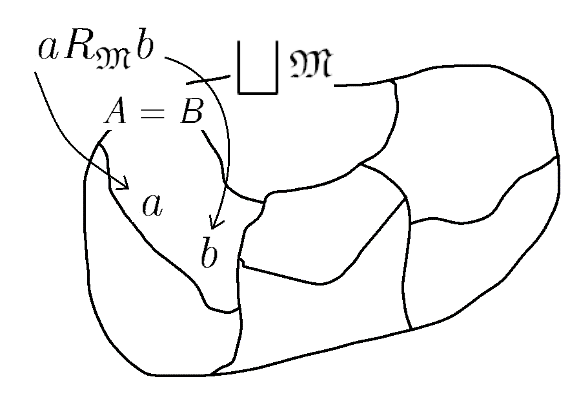
\includegraphics[width=160pt]{1.2.5.a.png}
\end{center}
\begin{dfn}
集合$A$の1つの同値関係$R$が与えられたとする。このとき、次式のような集合$C_{R}(a)$が定義されよう。
\begin{align*}
C_{R}(a) = \left\{ c \in A \middle| aRc \right\} \subseteq A
\end{align*}
この集合$C_{R}(a)$をその同値関係$R$によるその元$a$の同値類、または単に、類などといい$[ a]_{R}$、$\overline{a}$などとも書く。
\end{dfn}\par
このことは次のようにして考えられればわかりやすかろう。
\begin{center}
  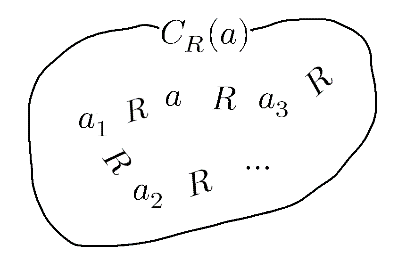
\includegraphics[width=160pt]{1.2.5.b.png}
\end{center}
\begin{thm}\label{8.1.4.29}
次のことが成り立つ。
\begin{itemize}
\item
  $\forall a \in A$に対し、$a \in C_{R}(a)$が成り立つ。
\item
  $\forall a,b \in A$に対し、$aRb$が成り立つならそのときに限り、$C_{R}(a) = C_{R}(b)$が成り立つ。
\item
  $\forall a,b \in A$に対し、$C_{R}(a) \neq C_{R}(b)$が成り立つなら、$C_{R}(a) \cap C_{R}(b) = \emptyset$が成り立つ。
\end{itemize}
\end{thm}
\begin{thm}\label{8.1.4.30}
集合$A$の1つの同値関係$R$が与えられたとする。次式のようにその同値関係$R$によるその元$a$の同値類全体の集合$\mathfrak{M}$が定義されると、
\begin{align*}
\mathfrak{M}=\left\{ C_{R}(a)\in \mathfrak{P}(A) \middle| C_{R}(a) = \left\{ c \in A \middle| aRc \right\} \right\}
\end{align*}
その集合$\mathfrak{M}$はその集合$A$の直和分割でこれに付随する同値関係$R_{\mathfrak{M}}$はその同値関係$R$に等しい。
\end{thm}\par
このことは次のようにして考えられればわかりやすかろう。
\begin{center}
    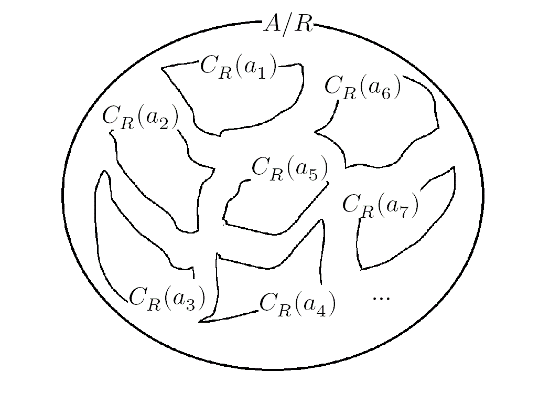
\includegraphics[width=160pt]{1.2.5.c.png}
\end{center}
\begin{dfn}
このようにして、その同値関係$R$からその集合$\mathfrak{M}$が定義されること、即ち、その集合$A$がその同値関係$R$によって得られる同値類たちの直和$\bigsqcup_{} \mathfrak{M}$とみなすことをその集合$A$のその同値関係$R$による類別、分類といいその集合$\mathfrak{M}$をその集合$A$のその同値関係による商集合といい$A/R$などと書く。
\end{dfn}
\begin{thm}\label{8.1.4.31}
ここで、写像$f:A \rightarrow B$が与えられたとする。このとき、その集合$A$の元々$a$、$b$に対し、次式のように論理式$aR(f)b$が定義されると、
\begin{align*}
aR(f)b \Leftrightarrow a,b \in A \land f(a) = f(b)
\end{align*}
その集合$A$における関係$R(f)$が得られこれは同値関係となる。
\end{thm}
\begin{dfn}
この関係$R(f)$をその写像$f$に付随する同値関係、その写像$f$の同値核などという。
\end{dfn}
\begin{thm}\label{8.1.4.32}
集合$A$の1つの同値関係$R$が与えられたとする。次式のように写像$C_{R}$が定義されるとき、
\begin{align*}
C_{R}:A \rightarrow A/R;a \mapsto C_{R}(a)
\end{align*}
その写像$C_{R}$は全射でありこれに付随する同値関係$R\left( C_{R} \right)$はその同値関係$R$に等しい。
\end{thm}
\begin{dfn}
このような写像$C_{R}$をその集合$A$からその集合$A/R$への標準的全射、自然な全射、商写像などという。
\end{dfn}
\end{comment}
\begin{dfn}
位相空間$\left( S,\mathfrak{O} \right)$と同値関係$R$が与えられたとき、その標準的全射$C_{R}:S \rightarrow {S}/{R};a \mapsto C_{R}(a)$を用いて次式のように集合$\overline{\mathfrak{O}}$が定義される。この集合$\overline{\mathfrak{O}}$を位相空間$\left( S.\mathfrak{O} \right)$の同値関係$R$における商位相という。
\begin{align*}
\overline{\mathfrak{O}} = \left\{ O \in \mathfrak{P}\left( {S}/{R} \right) \middle| V\left( C_{R}^{- 1}|O \right)\in \mathfrak{O} \right\}
\end{align*}
\end{dfn}
\begin{thm}\label{8.1.4.33}
組$\left( {S}/{R},\overline{\mathfrak{O}} \right)$は位相空間である。
\end{thm}
\begin{dfn}
この位相空間$\left( {S}/{R},\overline{\mathfrak{O}} \right)$を位相空間$\left( S.\mathfrak{O} \right)$の同値関係$R$における商位相空間という。
\end{dfn}
\begin{proof}
上記のように定義された組$\left( {S}/{R},\overline{\mathfrak{O}} \right)$において、次のようになることから、
\begin{align*}
V\left( C_{R}^{- 1}|{S}/{R} \right) = V\left( C_{R}^{- 1} \right) = D\left( C_{R} \right) = S,\ \ V\left( C_{R}^{- 1}|\emptyset \right) = \emptyset
\end{align*}
${S}/{R},\emptyset \in \overline{\mathfrak{O}}$が成り立つ。$\forall O,P \in \overline{\mathfrak{O}}$に対し、$V\left( C_{R}^{- 1}|O \right),V\left( C_{R}^{- 1}|P \right)\in \mathfrak{O}$が成り立つので、次のようになる。
\begin{align*}
V\left( C_{R}^{- 1}|O \right) \cap V\left( C_{R}^{- 1}|P \right) = V\left( C_{R}^{- 1}|O \cap P \right)\in \mathfrak{O}
\end{align*}
したがって、$O \cap P \in \overline{\mathfrak{O}}$が成り立つ。任意の添数集合$\varLambda$によって添数づけられたその商位相$\overline{\mathfrak{O}}$の族$\left\{ O_{\lambda} \right\}_{\scriptsize \begin{matrix}
\lambda \in \varLambda \\
\end{matrix}}$が与えられたとき、$\forall\lambda \in \varLambda$に対し、$V\left( C_{R}^{- 1}|O_{\lambda} \right)\in \mathfrak{O}$が成り立つので、次のようになる。
\begin{align*}
\bigcup_{\scriptsize \begin{matrix}
\lambda \in \varLambda \\
\end{matrix}} {V\left( C_{R}^{- 1}|O_{\lambda} \right)} = V\left( C_{R}^{- 1}|\bigcup_{\scriptsize \begin{matrix}
\lambda \in \varLambda \\
\end{matrix}} O_{\lambda} \right)\in \mathfrak{O}
\end{align*}
したがって、$\bigcup_{\scriptsize \begin{matrix}
\lambda \in \varLambda \\
\end{matrix}} O_{\lambda} \in \overline{\mathfrak{O}}$が成り立つ。以上より、その組$\left( {S}/{R},\overline{\mathfrak{O}} \right)$は位相空間である。
\end{proof}
\begin{thm}\label{8.1.4.34}
位相空間$\left( S.\mathfrak{O} \right)$の同値関係$R$における商位相空間$\left( {S}/{R},\overline{\mathfrak{O}} \right)$が与えられたとき、標準的全射$C_{R}:S \rightarrow {S}/{R};a \mapsto C_{R}(a)$はその位相空間$\left( S,\mathfrak{O} \right)$からその商位相空間$\left( {S}/{R},\overline{\mathfrak{O}} \right)$への連続写像である。
\end{thm}
\begin{proof}
位相空間$\left( S.\mathfrak{O} \right)$の同値関係$R$における商位相空間$\left( {S}/{R},\overline{\mathfrak{O}} \right)$が与えられたとき、その標準的全射$C_{R}:S \rightarrow {S}/{R};a \mapsto C_{R}(a)$について、商位相の定義より明らかに、$\forall O \in \overline{\mathfrak{O}}$に対し、$V\left( C_{R}^{- 1}|O \right)\in \mathfrak{O}$が成り立つので、その標準的全射$C_{R}:S \rightarrow {S}/{R};a \mapsto C_{R}(a)$はその位相空間$\left( S,\mathfrak{O} \right)$からその商位相空間$\left( {S}/{R},\overline{\mathfrak{O}} \right)$への連続写像である。
\end{proof}
\begin{thm}\label{8.1.4.35}
位相空間たち$\left( S,\mathfrak{O} \right)$、$\left( T,\mathfrak{P} \right)$とそれらの間の連続写像$f:S \rightarrow T$、その集合$S$におけるその写像$f$に付随する同値関係$R(f)$が与えられたとき、次式のような写像$\overline{f}$が定まりこれはその商位相空間$\left( {S}/{R(f)},\overline{\mathfrak{O}} \right)$からその位相空間$\left( T,\mathfrak{P} \right)$への連続写像となる。
\begin{align*}
\overline{f}:{S}/{R(f)} \rightarrow T;C_{R(f)}(a) \mapsto f(a)
\end{align*}
\end{thm}
\begin{proof}
位相空間たち$\left( S,\mathfrak{O} \right)$、$\left( T,\mathfrak{P} \right)$とそれらの間の連続写像$f:S \rightarrow T$、その集合$S$におけるその写像$f$に付随する同値関係$R(f)$が与えられたとき、次式のような対応$\overline{f}$について考えよう。
\begin{align*}
\overline{f} = \left( {S}/{R(f)},T,G \right),\ \ G = \left\{ \left( C_{R(f)}(a),b \right) \in {S}/{R(f)} \times T \middle| b = f(a) \right\}
\end{align*}
このとき、$\forall C_{R(f)}(a),C_{R(f)}(b) \in {S}/{R(f)}$に対し、$C_{R(f)}(a) = C_{R(f)}(b)$が成り立つなら、$aR(f)b$が成り立ち、したがって、$f(a) = f(b)$も成り立つ。したがって、その対応$\overline{f}$は写像である。このとき、標準的全射$C_{R(f)}:S \rightarrow {S}/{R(f)};a \mapsto C_{R(f)}(a)$を用いて$f = \overline{f} \circ C_{R(f)}$が成り立つことに注意すれば、$\forall P \in \mathfrak{P}$に対し、$V\left( f^{- 1}|P \right)\in \mathfrak{O}$が成り立ち、ここで、$f^{- 1} = C_{R(f)}^{- 1} \circ {\overline{f}}^{- 1}$が成り立つので、$V\left( C_{R(f)}^{- 1}|V\left( {\overline{f}}^{- 1}|P \right) \right)\in \mathfrak{O}$が成り立つ。したがって、定義より明らかにその同値関係$R$による商位相$\overline{\mathfrak{O}}$を用いて$V\left( {\overline{f}}^{- 1}|P \right) \in \overline{\mathfrak{O}}$が得られるので、その写像$\overline{f}$はその商位相空間$\left( {S}/{R(f)},\overline{\mathfrak{O}} \right)$からその位相空間$\left( T,\mathfrak{P} \right)$への連続写像となる。
\end{proof}
\begin{thm}\label{8.1.4.36}
位相空間たち$\left( S,\mathfrak{O} \right)$、$\left( T,\mathfrak{P} \right)$とそれらの間の連続写像$f:S \rightarrow T$、それらの集合たち$S$、$T$における同値関係たち$Q$、$R$が与えられ、$\forall a,b \in S$に対し、$aQb$が成り立つなら、$f(a)Rf(b)$が成り立つとき、次式のような写像$\overline{f}$が定まりこれはその商位相空間$\left( {S}/{Q},\overline{\mathfrak{O}} \right)$からその商位相空間$\left( {T}/{R},\overline{\mathfrak{P}} \right)$への連続写像となる。
\begin{align*}
\overline{f}:{S}/{Q} \rightarrow {T}/{R};C_{Q}(a) \mapsto C_{R} \circ f(a)
\end{align*}
\end{thm}
\begin{proof}
位相空間たち$\left( S,\mathfrak{O} \right)$、$\left( T,\mathfrak{P} \right)$とそれらの間の連続写像$f:S \rightarrow T$、それらの集合たち$S$、$T$における同値関係たち$Q$、$R$が与えられ、$\forall a,b \in S$に対し、$aQb$が成り立つなら、$f(a)Rf(b)$が成り立つとき、次式のような対応$\overline{f}$について考えよう。
\begin{align*}
\overline{f} = \left( {S}/{Q},{T}/{R},G \right),\ \ G = \left\{ \left( C_{Q}(a),C \right) \in {S}/{Q} \times {T}/{R} \middle| C = C_{R} \circ f(a) \right\}
\end{align*}
このとき、$\forall C_{Q}(a),C_{Q}(b) \in {S}/{Q}$に対し、$C_{Q}(a) = C_{Q}(b)$が成り立つなら、$aQb$が成り立ち、したがって、$f(a)Rf(b)$も成り立つので、$C_{R} \circ f(a) = C_{R} \circ f(b)$も成り立つ。したがって、その対応$\overline{f}$は写像である。ここで、定理\ref{8.1.4.34}よりその商位相空間$\left( {T}/{R},\overline{\mathfrak{P}} \right)$を用いた標準的全射$C_{R}:T \rightarrow {T}/{R};a \mapsto C_{R}(a)$はその位相空間$\left( T,\mathfrak{P} \right)$からその商位相空間$\left( {T}/{R},\overline{\mathfrak{P}} \right)$への連続写像となるのであった。このとき、その合成写像$C_{R} \circ f:S \rightarrow {T}/{R}$も連続写像で定理\ref{8.1.4.35}よりその写像$\overline{f}:{S}/{Q} \rightarrow {T}/{R};C_{Q}(a) \mapsto C_{R} \circ f(a)$も連続写像となる。
\end{proof}
\begin{thebibliography}{50}
\bibitem{1}
  松坂和夫, 集合・位相入門, 岩波書店, 1968. 新装版第2刷 p52-59,186-194 ISBN978-4-00-029871-1
\bibitem{2}
  加塩朋和. "一般位相A(2組)". 東京理科大学. \url{https://www.rs.tus.ac.jp/a25594/2018-2019_General_Topology.pdf} (2021-8-6 12:15 取得)
\end{thebibliography}
\end{document}

\clearpage
\documentclass[dvipdfmx]{jsarticle}
\setcounter{section}{1}
\setcounter{subsection}{4}
\usepackage{xr}
\externaldocument{8.1.1}
\usepackage{amsmath,amsfonts,amssymb,array,comment,mathtools,url,docmute}
\usepackage{longtable,booktabs,dcolumn,tabularx,mathtools,multirow,colortbl,xcolor}
\usepackage[dvipdfmx]{graphics}
\usepackage{bmpsize}
\usepackage{amsthm}
\usepackage{enumitem}
\setlistdepth{20}
\renewlist{itemize}{itemize}{20}
\setlist[itemize]{label=•}
\renewlist{enumerate}{enumerate}{20}
\setlist[enumerate]{label=\arabic*.}
\setcounter{MaxMatrixCols}{20}
\setcounter{tocdepth}{3}
\newcommand{\rotin}{\text{\rotatebox[origin=c]{90}{$\in $}}}
\newcommand{\amap}[6]{\text{\raisebox{-0.7cm}{\begin{tikzpicture} 
  \node (a) at (0, 1) {$\textstyle{#2}$};
  \node (b) at (#6, 1) {$\textstyle{#3}$};
  \node (c) at (0, 0) {$\textstyle{#4}$};
  \node (d) at (#6, 0) {$\textstyle{#5}$};
  \node (x) at (0, 0.5) {$\rotin $};
  \node (x) at (#6, 0.5) {$\rotin $};
  \draw[->] (a) to node[xshift=0pt, yshift=7pt] {$\textstyle{\scriptstyle{#1}}$} (b);
  \draw[|->] (c) to node[xshift=0pt, yshift=7pt] {$\textstyle{\scriptstyle{#1}}$} (d);
\end{tikzpicture}}}}
\newcommand{\twomaps}[9]{\text{\raisebox{-0.7cm}{\begin{tikzpicture} 
  \node (a) at (0, 1) {$\textstyle{#3}$};
  \node (b) at (#9, 1) {$\textstyle{#4}$};
  \node (c) at (#9+#9, 1) {$\textstyle{#5}$};
  \node (d) at (0, 0) {$\textstyle{#6}$};
  \node (e) at (#9, 0) {$\textstyle{#7}$};
  \node (f) at (#9+#9, 0) {$\textstyle{#8}$};
  \node (x) at (0, 0.5) {$\rotin $};
  \node (x) at (#9, 0.5) {$\rotin $};
  \node (x) at (#9+#9, 0.5) {$\rotin $};
  \draw[->] (a) to node[xshift=0pt, yshift=7pt] {$\textstyle{\scriptstyle{#1}}$} (b);
  \draw[|->] (d) to node[xshift=0pt, yshift=7pt] {$\textstyle{\scriptstyle{#2}}$} (e);
  \draw[->] (b) to node[xshift=0pt, yshift=7pt] {$\textstyle{\scriptstyle{#1}}$} (c);
  \draw[|->] (e) to node[xshift=0pt, yshift=7pt] {$\textstyle{\scriptstyle{#2}}$} (f);
\end{tikzpicture}}}}
\renewcommand{\thesection}{第\arabic{section}部}
\renewcommand{\thesubsection}{\arabic{section}.\arabic{subsection}}
\renewcommand{\thesubsubsection}{\arabic{section}.\arabic{subsection}.\arabic{subsubsection}}
\everymath{\displaystyle}
\allowdisplaybreaks[4]
\usepackage{vtable}
\theoremstyle{definition}
\newtheorem{thm}{定理}[subsection]
\newtheorem*{thm*}{定理}
\newtheorem{dfn}{定義}[subsection]
\newtheorem*{dfn*}{定義}
\newtheorem{axs}[dfn]{公理}
\newtheorem*{axs*}{公理}
\renewcommand{\headfont}{\bfseries}
\makeatletter
  \renewcommand{\section}{%
    \@startsection{section}{1}{\z@}%
    {\Cvs}{\Cvs}%
    {\normalfont\huge\headfont\raggedright}}
\makeatother
\makeatletter
  \renewcommand{\subsection}{%
    \@startsection{subsection}{2}{\z@}%
    {0.5\Cvs}{0.5\Cvs}%
    {\normalfont\LARGE\headfont\raggedright}}
\makeatother
\makeatletter
  \renewcommand{\subsubsection}{%
    \@startsection{subsubsection}{3}{\z@}%
    {0.4\Cvs}{0.4\Cvs}%
    {\normalfont\Large\headfont\raggedright}}
\makeatother
\makeatletter
\renewenvironment{proof}[1][\proofname]{\par
  \pushQED{\qed}%
  \normalfont \topsep6\p@\@plus6\p@\relax
  \trivlist
  \item\relax
  {
  #1\@addpunct{.}}\hspace\labelsep\ignorespaces
}{%
  \popQED\endtrivlist\@endpefalse
}
\makeatother
\renewcommand{\proofname}{\textbf{証明}}
\usepackage{tikz,graphics}
\usepackage[dvipdfmx]{hyperref}
\usepackage{pxjahyper}
\hypersetup{
 setpagesize=false,
 bookmarks=true,
 bookmarksdepth=tocdepth,
 bookmarksnumbered=true,
 colorlinks=false,
 pdftitle={},
 pdfsubject={},
 pdfauthor={},
 pdfkeywords={}}
\begin{document}
%\hypertarget{ux9023ux7d50}{%
\subsection{連結}%\label{ux9023ux7d50}}
%\hypertarget{ux9023ux7d50-1}{%
\subsubsection{連結}%\label{ux9023ux7d50-1}}
\begin{dfn}
任意の位相空間$\left( S,\mathfrak{O} \right)$が与えられたとする。これの台集合$S$、空集合$\emptyset$はどちらもその位相空間$\left( S,\mathfrak{O} \right)$の開集合でもあり閉集合でもあるのであった。ここで、その位相空間$\left( S,\mathfrak{O} \right)$の閉集合系$\mathfrak{A}$を用いて次式を満たすとき、その位相空間$\left( S,\mathfrak{O} \right)$は連結であるという\footnote{定義だけみるとなんじゃあこりゃって感じですが、解析学的にいえば、弧状連結という平たくいえば集合内のどの2点でもある曲線を集合内で引けるような感じの集合と似た概念なので、心象したいときはとりあえずこれでやるといいんじゃあないかなと思います。}。
\begin{align*}
\mathfrak{O \cap A} = \left\{ S,\emptyset \right\}
\end{align*}
\end{dfn}\par
たとえば、任意の密着位相は連結である。また、離散位相は台集合$S$がただ1点のみからなるときに限り連結である。
\begin{thm}\label{8.1.5.1}
位相空間$\left( S,\mathfrak{O} \right)$が連結であるならそのときに限り、その閉集合系$\mathfrak{A}$を用いて$S = M \sqcup N$なるその集合$\mathfrak{O \cap A}$の空集合でない元々$M$、$N$が存在しない。
\end{thm}
\begin{proof}
任意の位相空間$\left( S,\mathfrak{O} \right)$が与えられたとする。その位相空間$\left( S,\mathfrak{O} \right)$が連結でないなら、その閉集合系$\mathfrak{A}$を用いて$\mathfrak{O \cap A} =\left\{ S,\emptyset \right\}$が成り立たなく、その台集合$S$、空集合$\emptyset$はどちらもその位相空間$\left( S,\mathfrak{O} \right)$の開集合でもあり閉集合でもあることに注意すれば、$M\in \mathfrak{O \cap A}$なる集合$M$が存在する。ここで、その集合$S \setminus M$について、$M\in \mathfrak{O}$より$S \setminus M\in \mathfrak{A}$が成り立つかつ、$M\in \mathfrak{A}$より$S \setminus M\in \mathfrak{O}$が成り立つので、$S \setminus M\in \mathfrak{O \cap A}$が成り立つ。さらに、$M \cap S \setminus M = \emptyset$が成り立つので、$M \sqcup S \setminus M = S$が成り立つことになり$S = M \sqcup N$なるその集合$\mathfrak{O \cap A}$の空集合でない元々$M$、$N$が存在する。\par
逆に、$S = M \sqcup N$なるその集合$\mathfrak{O \cap A}$の空集合でない元々$M$、$N$が存在するなら、どちらも$M,N \notin \left\{ S,\emptyset \right\}$が成り立つので、$\mathfrak{O \cap A \neq}\left\{ S,\emptyset \right\}$が成り立つことになりその位相空間$\left( S,\mathfrak{O} \right)$は連結でない。
\end{proof}
\begin{thm}\label{8.1.5.2}
また、その位相空間$\left( S,\mathfrak{O} \right)$が与えられたとする。その台集合$S$の空集合でない部分集合$M$を用いた部分位相空間$\left( M,\mathfrak{O}_{M} \right)$が連結であるならそのときに限り、次式たちいづれもが成り立つようなその位相空間$\left( S,\mathfrak{O} \right)$の開集合たち$O$、$P$が存在しない。
\begin{align*}
M \subseteq O \cup P,\ \ O \cap P \cap M = \emptyset,\ \ O \cap M \neq \emptyset,\ \ P \cap M \neq \emptyset
\end{align*}
\end{thm}
\begin{proof}
任意の位相空間$\left( S,\mathfrak{O} \right)$が与えられたとする。その台集合の空集合でない部分集合$M$を用いたその位相空間$\left( S,\mathfrak{O} \right)$の部分位相空間$\left( M,\mathfrak{O}_{M} \right)$が連結でないなら、その閉集合系$\mathfrak{A}_{M}$を用いて$M = M' \sqcup N'$なるその集合$\mathfrak{O}_{M} \cap \mathfrak{A}_{M}$の空集合でない元々$M'$、$N'$が存在する。ここで定理8.1.4.8
より$\exists O,P \in \mathfrak{O}$に対し、$M' = O \cap M$かつ$N' = P \cap M$が成り立つので、次式たちいづれもが成り立つ。
\begin{align*}
M = (O \cap M) \cup (P \cap M),\ \ O \cap M \cap P \cap M = \emptyset
\end{align*}
したがって、$M \subseteq O \cup P$かつ$O \cap P \cap M = \emptyset$が得られる。また、それらの集合たち$M'$、$N'$は空集合でないので、それらの集合たち$O \cap M$、$P \cap M$は空集合でない。\par
逆に、次式たちいづれもが成り立つようなその位相空間$\left( S,\mathfrak{O} \right)$の開集合たち$O$、$P$が存在するなら、
\begin{align*}
M \subseteq O \cup P,\ \ O \cap P \cap M = \emptyset,\ \ O \cap M \neq \emptyset,\ \ P \cap M \neq \emptyset
\end{align*}
それらの集合たち$O \cap M$、$P \cap M$をそれぞれ$M'$、$N'$とおくと、$M',N' \in \mathfrak{O}_{M}$が成り立つかつ、それらの集合たち$M'$、$N'$は空集合でない。さらに、$M' \cap N' = \emptyset$が成り立ち、$M \subseteq O \cup P$が成り立つので、次のようになる。
\begin{align*}
M' \sqcup N' &= (O \cap M) \cup (P \cap M)\\
&= (O \cup P) \cap M\\
&= M
\end{align*}
したがって、次式が成り立つので、
\begin{align*}
M' = M \setminus N',\ \ N' = M \setminus M'
\end{align*}
$M',N' \in \mathfrak{O}_{M} \cap \mathfrak{A}_{M}$なるある集合たち$M'$、$N'$が$M' \sqcup N' = M$を満たす。これにより、その部分位相空間$\left( M,\mathfrak{O}_{M} \right)$は連結でない。
\end{proof}
\begin{thm}\label{8.1.5.3}
位相空間たち$\left( S,\mathfrak{O} \right)$、$\left( T,\mathfrak{P} \right)$が与えられたとする。その位相空間$\left( S,\mathfrak{O} \right)$は連結で写像$f:S \rightarrow T$がその位相空間$\left( S,\mathfrak{O} \right)$からその位相空間$\left( T,\mathfrak{P} \right)$へ連続であるとするとき、その位相空間$\left( T,\mathfrak{P} \right)$の部分位相空間$\left( V(f),\mathfrak{O}_{V(f)} \right)$は連結である。
\end{thm}
\begin{proof}
位相空間たち$\left( S,\mathfrak{O} \right)$、$\left( T,\mathfrak{P} \right)$が与えられたとする。その位相空間$\left( S,\mathfrak{O} \right)$は連結で写像$f:S \rightarrow T$がその位相空間$\left( S,\mathfrak{O} \right)$からその位相空間$\left( T,\mathfrak{P} \right)$へ連続であるとするとき、その位相空間$\left( T,\mathfrak{P} \right)$の部分位相空間$\left( V(f),\mathfrak{O}_{V(f)} \right)$が連結でないと仮定しよう。このとき、次式が成り立つような次式が成り立つようなその位相空間$\left( T,\mathfrak{P} \right)$の開集合たち$O$、$P$が存在する。
\begin{align*}
V(f) \subseteq O \cup P,\ \ O \cap P \cap V(f) = \emptyset,\ \ O \cap V(f) \neq \emptyset,\ \ P \cap V(f) \neq \emptyset
\end{align*}
ここで、次のようになるかつ、
\begin{align*}
V(f) \subseteq O \cup P &\Rightarrow V\left( f^{- 1}|V(f) \right) \subseteq V\left( f^{- 1}|O \cup P \right)\\
&\Rightarrow S \subseteq V\left( f^{- 1}|O \right) \cup V\left( f^{- 1}|P \right)
\end{align*}
値域の定義より$V\left( f^{- 1}|O \right) \subseteq P$かつ$V\left( f^{- 1}|P \right) \subseteq S$が成り立つので、$S = V\left( f^{- 1}|O \right) \cup V\left( f^{- 1}|P \right)$が成り立つ。また、値域の定義より$V\left( f^{- 1}|O \right) \subseteq S$かつ$V\left( f^{- 1}|P \right) \subseteq S$が成り立つことに注意すれば、次のようになるかつ、
\begin{align*}
O \cap P \cap V(f) = \emptyset &\Rightarrow V\left( f^{- 1}|O \cap P \cap V(f) \right) = V\left( f^{- 1}|\emptyset \right) = \emptyset\\
&\Leftrightarrow V\left( f^{- 1}|O \right) \cap V\left( f^{- 1}|P \right) \cap V\left( f^{- 1}|V(f) \right) = \emptyset\\
&\Rightarrow V\left( f^{- 1}|O \right) \cap V\left( f^{- 1}|P \right) \cap S \subseteq \emptyset\\
&\Rightarrow V\left( f^{- 1}|O_{1} \right) \cap V\left( f^{- 1}|O_{2} \right) \subseteq \emptyset
\end{align*}
空集合はいかなる集合の部分集合であるのであったので、$V\left( f^{- 1}|O \right) \cap V\left( f^{- 1}|P \right) = \emptyset$が成り立つ。以上より、$S = V\left( f^{- 1}|O \right) \sqcup V\left( f^{- 1}|P \right)$が成り立つ。\par
さらに、$O \cap V(f) \neq \emptyset$が成り立つので、$\exists b \in S$に対し、$b \in O \cap V(f)$が成り立ち、$b \in V(f)$より$\exists a \in S$に対し、$f(a) = b$が成り立つ。これにより、明らかに$a \in S$が成り立つかつ、$\exists b \in O \cap V(f)$に対し、$f(a) = b$が成り立つので、定義より$a \in V\left( f^{- 1}|O \cap V(f) \right)$が成り立つ。ここで、次式が成り立つので、
\begin{align*}
V\left( f^{- 1}|O \cap V(f) \right) &= V\left( f^{- 1}|O \right) \cap V\left( f^{- 1}|V(f) \right)\\
&= V\left( f^{- 1}|O \right) \cap S\\
&= V\left( f^{- 1}|O \right)
\end{align*}
$V\left( f^{- 1}|O \right) \neq \emptyset$が成り立つ。同様にして、$V\left( f^{- 1}|P \right) \neq \emptyset$が成り立つ。\par
ここで、その写像$f$は連続であったので、$V\left( f^{- 1}|O \right),V\left( f^{- 1}|P \right) \in \mathfrak{O}$が成り立つ。$S = V\left( f^{- 1}|O \right) \sqcup V\left( f^{- 1}|P \right)$が成り立つことに注意すれば、$S \setminus V\left( f^{- 1}|O \right) = V\left( f^{- 1}|P \right)$かつ$S \setminus V\left( f^{- 1}|P \right) = V\left( f^{- 1}|O \right)$が成り立つので、その位相空間$\left( S,\mathfrak{O} \right)$の閉集合系$\mathfrak{A}$を用いて$V\left( f^{- 1}|O \right),V\left( f^{- 1}|P \right) \in \mathfrak{A}$が成り立つことになり、したがって、$V\left( f^{- 1}|O \right),V\left( f^{- 1}|P \right) \in \mathfrak{O} \cap \mathfrak{A}$が成り立つ。これにより、その位相空間$\left( S,\mathfrak{O} \right)$は連結でない。しかしながら、これは仮定に矛盾するので、その位相空間$\left( T,\mathfrak{P} \right)$の部分位相空間$\left( V(f),\mathfrak{O}_{V(f)} \right)$は連結である。
\end{proof}
\begin{thm}\label{8.1.5.4}
位相空間たち$\left( S,\mathfrak{O} \right)$、$\left( T,\mathfrak{P} \right)$が与えられたとする。その台集合$S$の空集合でない部分集合$M$を用いたその位相空間$\left( S,\mathfrak{O} \right)$の部分位相空間$\left( M,\mathfrak{O}_{M} \right)$は連結で写像$f:S \rightarrow T$がその位相空間$\left( S,\mathfrak{O} \right)$からその位相空間$\left( T,\mathfrak{P} \right)$へ連続であるとするとき、その位相空間$\left( T,\mathfrak{P} \right)$の部分位相空間$\left( V\left( f|M \right),\mathfrak{O}_{V\left( f|M \right)} \right)$は連結である。
\end{thm}
\begin{proof}
位相空間たち$\left( S,\mathfrak{O} \right)$、$\left( T,\mathfrak{P} \right)$が与えられたとする。その台集合$S$の空集合でない部分集合$M$を用いたその位相空間$\left( S,\mathfrak{O} \right)$の部分位相空間$\left( M,\mathfrak{O}_{M} \right)$は連結で写像$f:S \rightarrow T$がその位相空間$\left( S,\mathfrak{O} \right)$からその位相空間$\left( T,\mathfrak{P} \right)$へ連続であるとするとき、その部分集合$M$に制限されたその写像$f|M$もまたその位相空間$\left( M,\mathfrak{O}_{M} \right)$からその位相空間$\left( T,\mathfrak{P} \right)$へ連続であるので、上記の定理よりその位相空間$\left( T,\mathfrak{P} \right)$の部分位相空間$\left( V\left( f|M \right),\mathfrak{O}_{V\left( f|M \right)} \right)$は連結である。
\end{proof}
\begin{thm}\label{8.1.5.5}
位相空間$\left( S,\mathfrak{O} \right)$の台集合$S$の空集合でない部分集合$M$を用いた部分位相空間$\left( M,\mathfrak{O}_{M} \right)$が連結であるなら、$\forall N \in \mathfrak{P}(S)$に対し、$M \subseteq N \subseteq {\mathrm{cl}}M$が成り立つなら、その部分位相空間$\left( N,\mathfrak{O}_{N} \right)$も連結である。
\end{thm}
\begin{proof}
位相空間$\left( S,\mathfrak{O} \right)$の台集合$S$の空集合でない部分集合$M$を用いた部分位相空間$\left( M,\mathfrak{O}_{M} \right)$が連結であるかつ、$\exists N \in \mathfrak{P}(S)$に対し、$M \subseteq N \subseteq {\mathrm{cl}}M$が成り立つかつ、その部分位相空間$\left( N,\mathfrak{O}_{N} \right)$が連結でないと仮定しよう。このとき、$\exists O,P \in \mathfrak{O}$に対し、次式が成り立つ。
\begin{align*}
N \subseteq O \cup P,\ \ O \cap P \cap N = \emptyset,\ \ O \cap N \neq \emptyset,\ \ P \cap N \neq \emptyset
\end{align*}
$M \subseteq N$が成り立つので、次式が成り立つ。
\begin{align*}
M \subseteq O \cup P,\ \ O \cap P \cap M = \emptyset
\end{align*}
また、$O \cap M = \emptyset$が成り立つと仮定すると、定理\ref{8.1.1.10}より$O \cap {\mathrm{cl}}M = \emptyset$が成り立ち、したがって、$O \cap N = \emptyset$が成り立つことになるが、これは$O \cap N \neq \emptyset$が成り立つことに矛盾するので、$O \cap M \neq \emptyset$が成り立つ。同様にして、$O \cap M \neq \emptyset$が得られる。以上より、次式が得られ、
\begin{align*}
M \subseteq O \cup P,\ \ O \cap P \cap M = \emptyset,\ \ O \cap M \neq \emptyset,\ \ P \cap M \neq \emptyset
\end{align*}
これにより、その部分位相空間$\left( N,\mathfrak{O}_{N} \right)$は連結でないことになるが、これはその部分位相空間$\left( M,\mathfrak{O}_{M} \right)$が連結であるに矛盾している。よって、その部分位相空間$\left( N,\mathfrak{O}_{N} \right)$も連結である。
\end{proof}
\begin{thm}\label{8.1.5.6}
位相空間$\left( S,\mathfrak{O} \right)$の台集合$S$の添数集合$\varLambda$によって添数づけられた部分集合系$\left\{ M_{\lambda} \right\}_{\lambda \in \varLambda}$を用いた部分位相空間の族$\left\{ \left( M_{\lambda},\mathfrak{O}_{M_{\lambda}} \right) \right\}_{\lambda \in \varLambda}$が与えられたとする。$\forall\lambda \in \varLambda$に対し、それらの部分位相空間たち$\left( M_{\lambda},\mathfrak{O}_{M_{\lambda}} \right)$が連結であるかつ、$\forall\lambda,\mu \in \varLambda$に対し、$M_{\lambda} \cap M_{\mu} \neq \emptyset$が成り立つとき、その和集合$\bigcup_{\lambda \in \varLambda} M_{\lambda}$を用いた部分位相空間$\left( \bigcup_{\lambda \in \varLambda} M_{\lambda},\mathfrak{O}_{\bigcup_{\lambda \in \varLambda} M_{\lambda}} \right)$も連結である。
\end{thm}
\begin{proof}
位相空間$\left( S,\mathfrak{O} \right)$の台集合$S$の添数集合$\varLambda$によって添数づけられた部分集合系$\left\{ M_{\lambda} \right\}_{\lambda \in \varLambda}$を用いた部分位相空間の族$\left\{ \left( M_{\lambda},\mathfrak{O}_{M_{\lambda}} \right) \right\}_{\lambda \in \varLambda}$が与えられたとする。$\forall\lambda \in \varLambda$に対し、それらの部分位相空間たち$\left( M_{\lambda},\mathfrak{O}_{M_{\lambda}} \right)$が連結であるかつ、$\forall\lambda,\mu \in \varLambda$に対し、$M_{\lambda} \cap M_{\mu} \neq \emptyset$が成り立つかつ、その和集合$\bigcup_{\lambda \in \varLambda} M_{\lambda}$を用いた部分位相空間$\left( \bigcup_{\lambda \in \varLambda} M_{\lambda},\mathfrak{O}_{\bigcup_{\lambda \in \varLambda} M_{\lambda}} \right)$は連結でないと仮定しよう。このとき、$\exists O,P \in \mathfrak{O}$に対し、次式が成り立つ。
\begin{align*}
\bigcup_{\lambda \in \varLambda} M_{\lambda} \subseteq O \cup P,\ \ O \cap P \cap \bigcup_{\lambda \in \varLambda} M_{\lambda} = \emptyset,\ \ O \cap \bigcup_{\lambda \in \varLambda} M_{\lambda} \neq \emptyset,\ \ P \cap \bigcup_{\lambda \in \varLambda} M_{\lambda} \neq \emptyset
\end{align*}
$\forall\lambda \in \varLambda$に対し、$M_{\lambda} \subseteq \bigcup_{\lambda \in \varLambda} M_{\lambda}$が成り立つので、$\forall\lambda \in \varLambda$に対し、次式が成り立つ。
\begin{align*}
M_{\lambda} \subseteq O \cup P,\ \ O \cap P \cap M_{\lambda} = \emptyset
\end{align*}
ここで、$O \cap \bigcup_{\lambda \in \varLambda} M_{\lambda} \neq \emptyset$が成り立つので、$\exists a \in S$に対し、次のようになり、
\begin{align*}
a \in O \cap \bigcup_{\lambda \in \varLambda} M_{\lambda} = \bigcup_{\lambda \in \varLambda} \left( O \cap M_{\lambda} \right)
\end{align*}
$\exists\lambda \in \varLambda$に対し、$a \in O \cap M_{\lambda}$が成り立ち、したがって、$O \cap M_{\lambda} \neq \emptyset$が成り立つ。同様にして、$\exists\mu \in \varLambda$に対し、$P \cap M_{\mu} \neq \emptyset$が成り立つ。ここで、それらの部分位相空間たち$\left( M_{\lambda},\mathfrak{O}_{M_{\lambda}} \right)$、$\left( M_{\mu},\mathfrak{O}_{M_{\mu}} \right)$が連結であるので、$O_{1} \cap M_{\mu} = \emptyset$かつ$O_{2} \cap M_{\lambda} = \emptyset$が成り立つ。これにより、次式が成り立つ。
\begin{align*}
\emptyset &= \left( \emptyset \cap M_{\lambda} \right) \cup \left( \emptyset \cap M_{\mu} \right)\\
&= \left( O \cap M_{\lambda} \cap M_{\mu} \right) \cup \left( P \cap M_{\lambda} \cap M_{\mu} \right)\\
&= (O \cup P) \cap \left( M_{\lambda} \cap M_{\mu} \right)
\end{align*}
ここで、$M_{\lambda} \cap M_{\mu} \subseteq \bigcup_{\lambda \in \varLambda} M_{\lambda} \subseteq O \cup P$が成り立つので、次式が成り立つ。
\begin{align*}
\emptyset &= (O \cup P) \cap \left( M_{\lambda} \cap M_{\mu} \right)\\
&= M_{\lambda} \cap M_{\mu}
\end{align*}
しかしながら、これは仮定の、$\forall\lambda,\mu \in \varLambda$に対し、$M_{\lambda} \cap M_{\mu} \neq \emptyset$が成り立つことに矛盾しているので、その和集合$\bigcup_{\lambda \in \varLambda} M_{\lambda}$を用いた部分位相空間$\left( \bigcup_{\lambda \in \varLambda} M_{\lambda},\mathfrak{O}_{\bigcup_{\lambda \in \varLambda} M_{\lambda}} \right)$も連結である。
\end{proof}
\begin{thm}\label{8.1.5.7}
位相空間$\left( S,\mathfrak{O} \right)$の台集合$S$の添数集合$\varLambda$によって添数づけられた部分集合系$\left\{ M_{\lambda} \right\}_{\lambda \in \varLambda}$を用いた部分位相空間の族$\left\{ \left( M_{\lambda},\mathfrak{O}_{M_{\lambda}} \right) \right\}_{\lambda \in \varLambda}$が与えられたとする。$\forall\lambda \in \varLambda$に対し、それらの部分位相空間たち$\left( M_{\lambda},\mathfrak{O}_{M_{\lambda}} \right)$が連結であるかつ、$\exists a \in S$に対し、$a \in M_{\lambda}$が成り立つとき、その和集合$\bigcup_{\lambda \in \varLambda} M_{\lambda}$を用いた部分位相空間$\left( \bigcup_{\lambda \in \varLambda} M_{\lambda},\mathfrak{O}_{\bigcup_{\lambda \in \varLambda} M_{\lambda}} \right)$も連結である。
\end{thm}
\begin{proof}
位相空間$\left( S,\mathfrak{O} \right)$の台集合$S$の添数集合$\varLambda$によって添数づけられた部分集合系$\left\{ M_{\lambda} \right\}_{\lambda \in \varLambda}$を用いた部分位相空間の族$\left\{ \left( M_{\lambda},\mathfrak{O}_{M_{\lambda}} \right) \right\}_{\lambda \in \varLambda}$が与えられたとする。$\forall\lambda \in \varLambda$に対し、それらの部分位相空間たち$\left( M_{\lambda},\mathfrak{O}_{M_{\lambda}} \right)$が連結であるかつ、$\exists a \in S$に対し、$a \in M_{\lambda}$が成り立つとき、$\forall\lambda,\mu \in \varLambda$に対し、$a \in M_{\lambda} \cap M_{\mu}$が成り立つので、$M_{\lambda} \cap M_{\mu} \neq \emptyset$が成り立ち、したがって、その和集合$\bigcup_{\lambda \in \varLambda} M_{\lambda}$を用いた部分位相空間$\left( \bigcup_{\lambda \in \varLambda} M_{\lambda},\mathfrak{O}_{\bigcup_{\lambda \in \varLambda} M_{\lambda}} \right)$も連結である。
\end{proof}
%\hypertarget{ux9023ux7d50ux6210ux5206}{%
\subsubsection{連結成分}%\label{ux9023ux7d50ux6210ux5206}}
\begin{dfn}
任意の位相空間$\left( S,\mathfrak{O} \right)$が与えられたとする。このとき、$a,b \in S$なる元々$a$、$b$が属するようなその位相空間$\left( S,\mathfrak{O} \right)$の連結な部分位相空間$\left( M,\mathfrak{O}_{M} \right)$の台集合$M$が存在するとき、このことを$a \sim_{\left( S,\mathfrak{O} \right)}b$と書くことにする。
\end{dfn}
\begin{thm}\label{8.1.5.8}
その関係$\sim_{\left( S,\mathfrak{O} \right)}$は同値関係となる。\par
このようにして、その集合$S$を同値関係$\sim_{\left( S,\mathfrak{O} \right)}$で類別して得られる商集合$\frac{S}{\sim_{\left( S,\mathfrak{O} \right)}}$の元をその位相空間$\left( S,\mathfrak{O} \right)$の連結成分という。
\end{thm}
\begin{proof}
任意の位相空間$\left( S,\mathfrak{O} \right)$が与えられたとする。\par
$\forall a \in S$に対し、位相空間$\left( \left\{ a \right\},\left\{ \emptyset,\left\{ a \right\} \right\} \right)$が考えれられれば、これは明らかにその位相空間$\left( S,\mathfrak{O} \right)$の部分位相空間であるかつ、上記の定理より明らかにその位相空間$\left( \left\{ a \right\},\left\{ \emptyset,\left\{ a \right\} \right\} \right)$は連結である。したがって、$a \sim_{\left( S,\mathfrak{O} \right)}a$が成り立つ。\par
また、$\forall a,b \in S$に対し、定義より明らかに$a \sim_{\left( S,\mathfrak{O} \right)}b$が成り立つなら、$b \sim_{\left( S,\mathfrak{O} \right)}a$が成り立つ。\par
最後に、$\forall a,b,c \in S$に対し、$a \sim_{\left( S,\mathfrak{O} \right)}b$かつ$b \sim_{\left( S,\mathfrak{O} \right)}c$が成り立つなら、それらの元々$a$、$b$が属するようなその位相空間$\left( S,\mathfrak{O} \right)$の連結な部分位相空間$\left( M,\mathfrak{O}_{M} \right)$の台集合$M$が存在するかつ、それらの元々$b$、$c$が属するようなその位相空間$\left( S,\mathfrak{O} \right)$の連結な部分位相空間$\left( N,\mathfrak{O}_{N} \right)$の台集合$N$が存在することになる。ここで、$b \in M$かつ$b \in N$が成り立つので、部分位相空間$\left( M \cup N,\mathfrak{O}_{M \cup N} \right)$も連結であることになる。このとき、$a,c \in M \cup N$が成り立つので、$a \sim_{\left( S,\mathfrak{O} \right)}c$が成り立つ。
\end{proof}
\begin{thm}\label{8.1.5.9}
位相空間$\left( S,\mathfrak{O} \right)$の台集合$S$の元$a$が属する連結成分を$C_{a}$とおく。その元$a$を含むその位相空間$\left( S,\mathfrak{O} \right)$の連結な任意の部分位相空間の台集合全体の集合を$\mathcal{C}_{\left( S,\mathfrak{O} \right),a}$とすれば、順序集合$\left( \mathcal{C}_{\left( S,\mathfrak{O} \right),a}, \subseteq \right)$においてその連結成分$C_{a}$は最大元となる。さらに、その連結成分$C_{a}$はその位相空間$\left( S,\mathfrak{O} \right)$において閉集合である。
\end{thm}
\begin{proof}
位相空間$\left( S,\mathfrak{O} \right)$の台集合$S$の元$a$が属する連結成分を$C_{a}$とおく。その元$a$を含むその位相空間$\left( S,\mathfrak{O} \right)$の連結な任意の部分位相空間の台集合全体の集合を$\mathcal{C}_{\left( S,\mathfrak{O} \right),a}$とすれば、$\forall M \in \mathcal{C}_{\left( S,\mathfrak{O} \right),a}$に対し、その位相空間$\left( S,\mathfrak{O} \right)$の部分位相空間たち$\left( M,\mathfrak{O}_{M} \right)$は定義より連結であるかつ、定義より$a \in M$が成り立つので、和集合$\bigcup_{} \mathcal{C}_{\left( S,\mathfrak{O} \right),a}$を用いた部分位相空間$\left( \bigcup_{} \mathcal{C}_{\left( S,\mathfrak{O} \right),a},\mathfrak{O}_{\bigcup_{} \mathcal{C}_{\left( S,\mathfrak{O} \right),a}} \right)$も連結であるので、明らかに$\bigcup_{} \mathcal{C}_{\left( S,\mathfrak{O} \right),a} \in \mathcal{C}_{\left( S,\mathfrak{O} \right),a}$が成り立つ。さらに、$\forall M \in \mathcal{C}_{\left( S,\mathfrak{O} \right),a}$に対し、$M \subseteq \bigcup_{} \mathcal{C}_{\left( S,\mathfrak{O} \right),a}$が成り立つので、順序集合$\left( \mathcal{C}_{\left( S,\mathfrak{O} \right),a}, \subseteq \right)$において、その集合$\bigcup_{M \in \mathcal{C}_{\left( S,\mathfrak{O} \right),a}} M$は最大元となる。\par
一方で、$\forall b \in \bigcup_{} \mathcal{C}_{\left( S,\mathfrak{O} \right),a}$に対し、$a,b \in \bigcup_{} \mathcal{C}_{\left( S,\mathfrak{O} \right),a}$が成り立つので、$a \sim_{\left( S,\mathfrak{O} \right)}b$が成り立ち、したがって、$b \in C_{a}$が成り立つ。これにより、$\bigcup_{} \mathcal{C}_{\left( S,\mathfrak{O} \right),a} \subseteq C_{a}$が得られる。さらに、$\forall b \in C_{a}$に対し、$a \sim_{\left( S,\mathfrak{O} \right)}b$が成り立つことになるので、それらの元々$a$、$b$が属するようなその位相空間$\left( S,\mathfrak{O} \right)$の連結な部分位相空間$\left( M',\mathfrak{O}_{M'} \right)$の台集合$M'$が存在し、明らかに、$M' \in \mathcal{C}_{\left( S,\mathfrak{O} \right),a}$が成り立つことになる。以上より、次式が得られる。
\begin{align*}
C_{a} \subseteq M' \subseteq \bigcup_{M \in \mathcal{C}_{\left( S,\mathfrak{O} \right),a}} M = \bigcup_{} \mathcal{C}_{\left( S,\mathfrak{O} \right),a}
\end{align*}
これにより、$\bigcup_{} \mathcal{C}_{\left( S,\mathfrak{O} \right),a} = C_{a}$が成り立つことになり順序集合$\left( \mathcal{C}_{\left( S,\mathfrak{O} \right),a}, \subseteq \right)$においてその集合$C_{a}$は最大元となる。\par
また、$\bigcup_{} \mathcal{C}_{\left( S,\mathfrak{O} \right),a} = C_{a}$が成り立つことに注意すれば、部分位相空間$\left( C_{a},\mathfrak{O}_{C_{a}} \right)$が連結であるなら、$C_{a} \subseteq M \subseteq {\mathrm{cl}}C_{a}$なるその台集合$S$の任意の部分集合$M$を用いた部分位相空間$\left( M,\mathfrak{O}_{M} \right)$も連結であるのであったので、その部分位相空間$\left( {\mathrm{cl}}C_{a},\mathfrak{O}_{{\mathrm{cl}}C_{a}} \right)$も連結であることになり、したがって、$C_{a} \subseteq {\mathrm{cl}}C_{a} \in \mathcal{C}_{\left( S,\mathfrak{O} \right),a}$が成り立つ。ここで、その連結成分$C_{a}$がその順序集合$\left( \mathcal{C}_{\left( S,\mathfrak{O} \right),a}, \subseteq \right)$において最大元となることに注意すれば、${\mathrm{cl}}C_{a} \subseteq C_{a}$が成り立ち、したがって、$C_{a} = {\mathrm{cl}}C_{a}$が成り立つ。これにより、その連結成分$C_{a}$は閉集合である。
\end{proof}
\begin{thm}\label{8.1.5.10}
位相空間$\left( S,\mathfrak{O} \right)$が連結であるならそのときに限り、その位相空間$\left( S,\mathfrak{O} \right)$はただ1つの連結成分をもちこれがその台集合$S$自身となる。
\end{thm}
\begin{proof}
位相空間$\left( S,\mathfrak{O} \right)$が連結であるなら、位相空間$\left( S,\mathfrak{O} \right)$の台集合$S$の元$a$が属する連結成分を$C_{a}$とおき、その元$a$を含むその位相空間$\left( S,\mathfrak{O} \right)$の連結な任意の部分位相空間の台集合全体の集合を$\mathcal{C}_{\left( S,\mathfrak{O} \right),a}$とすれば、順序集合$\left( \mathcal{C}_{\left( S,\mathfrak{O} \right),a}, \subseteq \right)$においてその連結成分$C_{a}$は最大元となるのであった。このとき、順序集合$\left( \mathcal{C}_{\left( S,\mathfrak{O} \right),a}, \subseteq \right)$において、$S \in \mathcal{C}_{\left( S,\mathfrak{O} \right),a}$が成り立つので、明らかに$C_{a} = S$が成り立つ。これ以外にその位相空間$\left( S,\mathfrak{O} \right)$の連結成分$C$が存在すれば、商集合の定義より$C \sqcup C_{a} \subseteq S$が成り立ち$C \sqcup S \subseteq S$が成り立つことになるが、これは矛盾している。したがって、その位相空間$\left( S,\mathfrak{O} \right)$はただ1つの連結成分をもちこれがその台集合$S$自身となる。逆に、その位相空間$\left( S,\mathfrak{O} \right)$はただ1つの連結成分をもちこれがその台集合$S$自身となるなら、明らかに位相空間$\left( S,\mathfrak{O} \right)$が連結である。
\end{proof}
%\hypertarget{ux76f4ux7a4dux4f4dux76f8ux7a7aux9593ux3068ux9023ux7d50}{%
\subsubsection{直積位相空間と連結}%\label{ux76f4ux7a4dux4f4dux76f8ux7a7aux9593ux3068ux9023ux7d50}}
\begin{thm}\label{8.1.5.11}
添数集合$\varLambda$によって添数づけられた位相空間の族$\left\{ \left( S_{\lambda},\mathfrak{O}_{\lambda} \right) \right\}_{\lambda \in \varLambda}$の直積位相空間$\left( \prod_{\lambda \in \varLambda} S_{\lambda},\mathfrak{O} \right)$が連結であるならそのときに限り、$\forall\lambda \in \varLambda$に対し、それらの位相空間たち$\left( S_{\lambda},\mathfrak{O}_{\lambda} \right)$が連結である。
\end{thm}
\begin{proof}
添数集合$\varLambda$によって添数づけられた位相空間の族$\left\{ \left( S_{\lambda},\mathfrak{O}_{\lambda} \right) \right\}_{\lambda \in \varLambda}$の直積位相空間$\left( \prod_{\lambda \in \varLambda} S_{\lambda},\mathfrak{O} \right)$が連結であるなら、$\forall\lambda \in \varLambda$に対し、射影たち${\mathrm{pr}}_{\lambda}:\prod_{\lambda \in \varLambda} S_{\lambda} \rightarrow S_{\lambda}$は定義より明らかに連続写像で、このとき、その位相空間$\left( S_{\lambda},\mathfrak{O}_{\lambda} \right)$の部分位相空間$\left( V\left( {\mathrm{pr}}_{\lambda} \right),\mathfrak{O}_{V\left( {\mathrm{pr}}_{\lambda} \right)} \right)$は連結であるのであった。このとき、それらの射影たち${\mathrm{pr}}_{\lambda}$の定義より明らかに$V\left( {\mathrm{pr}}_{\lambda} \right) = S_{\lambda}$が成り立ち、さらに、その直積位相$\mathfrak{O}$はその直積位相空間$\left( \prod_{\lambda \in \varLambda} S_{\lambda},\mathfrak{O}_{0} \right)$の初等開集合全体の集合が1つの開基となるので、これの和集合に制限されたそれらの射影たち${\mathrm{pr}}_{\lambda}$の値域がそれらの位相空間たち$\left( S_{\lambda},\mathfrak{O}_{\lambda} \right)$の開集合$O_{\lambda}$となることに注意すれば、やはり$\mathfrak{O}_{V\left( {\mathrm{pr}}_{\lambda} \right)} = \mathfrak{O}_{\lambda}$が成り立つ。以上より、その位相空間$\left( S_{\lambda},\mathfrak{O}_{\lambda} \right)$は連結である。\par
逆に、$\forall\lambda \in \varLambda$に対し、それらの位相空間たち$\left( S_{\lambda},\mathfrak{O}_{\lambda} \right)$が連結であるなら、$\varLambda = \left\{ 1,2 \right\}$のとき、$\forall\left( a_{1},a_{2} \right),\left( b_{1},b_{2} \right) \in S_{1} \times S_{2}$に対し、次式が成り立つので、
\begin{align*}
\left( S_{1},\mathfrak{O}_{1} \right) \approx \left( S_{1} \times \left\{ b_{2} \right\},\mathfrak{O}_{1}' \right) \land \left( S_{2},\mathfrak{O}_{2} \right) \approx \left( \left\{ a_{1} \right\} \times S_{2},\mathfrak{O}_{2}' \right)
\end{align*}
直積位相空間たち$\left( S_{1} \times \left\{ b_{2} \right\},\mathfrak{O}_{1}' \right)$、$\left( \left\{ a_{1} \right\} \times S_{2},\mathfrak{O}_{2}' \right)$はいずれも連結で、$\left( a_{1},b_{2} \right) \in \left( S_{1} \times \left\{ b_{2} \right\} \right) \cap \left( \left\{ a_{1} \right\} \times S_{2} \right)$が成り立つので、$\left( S_{1} \times \left\{ b_{2} \right\} \right) \cap \left( \left\{ a_{1} \right\} \times S_{2} \right) \neq \emptyset$が成り立つ。これにより、部分位相空間$\left( \left( S_{1} \times \left\{ b_{2} \right\} \right) \cup \left( \left\{ a_{1} \right\} \times S_{2} \right),\mathfrak{O}' \right)$も連結となり、明らかに$\left( a_{1},a_{2} \right),\left( b_{1},b_{2} \right) \in \left( S_{1} \times \left\{ b_{2} \right\} \right) \cup \left( \left\{ a_{1} \right\} \times S_{2} \right)$が成り立つので、次式が成り立つ。
\begin{align*}
\left( a_{1},a_{2} \right) \sim_{\left( S_{1} \times S_{2},\mathfrak{O} \right)}\left( b_{1},b_{2} \right)
\end{align*}
ここで、その位相空間$\left( S_{1} \times S_{2},\mathfrak{O} \right)$はただ1つの連結成分をもちこれがその台集合$S$自身となるので、その位相空間$\left( S_{1} \times S_{2},\mathfrak{O} \right)$も連結である。あとは数学的帰納法によって、一般に${\#}\varLambda < \aleph_{0}$なる添数集合$\varLambda$に対しても、$\forall\lambda \in \varLambda$に対し、それらの位相空間たち$\left( S_{\lambda},\mathfrak{O}_{\lambda} \right)$が連結であるなら、その直積位相空間$\left( \prod_{\lambda \in \varLambda} S_{\lambda},\mathfrak{O} \right)$も連結である。\par
さらに、任意の添数集合$\varLambda$において、$\forall\left( a_{\lambda}' \right)_{\lambda \in \varLambda} \in \prod_{\lambda \in \varLambda} S_{\lambda}$に対し、その添数集合$\varLambda$の部分集合のうち有限集合であるもの全体の集合を$\varOmega$とおくとする。$\forall\varLambda' \in \varOmega$に対し、次式が成り立つかつ、
\begin{align*}
\prod_{\lambda \in \varLambda'} S_{\lambda} \times \prod_{\lambda \in \varLambda \setminus \varLambda'} \left\{ a_{\lambda}' \right\} \approx \prod_{\lambda \in \varLambda'} S_{\lambda}
\end{align*}
${\#}\varLambda' < \aleph_{0}$が成り立つので、その直積位相空間$\left( \prod_{\lambda \in \varLambda'} S_{\lambda} \times \prod_{\lambda \in \varLambda \setminus \varLambda'} \left\{ a_{\lambda}' \right\},\mathfrak{O}_{\varLambda'}' \right)$も連結である。このような族$\left\{ \left( \prod_{\lambda \in \varLambda'} S_{\lambda} \times \prod_{\lambda \in \varLambda \setminus \varLambda'} \left\{ a_{\lambda}' \right\},\mathfrak{O}_{\varLambda'}' \right) \right\}_{\varLambda' \in \varOmega}$がその直積位相空間$\left( \prod_{\lambda \in \varLambda} S_{\lambda},\mathfrak{O} \right)$の連結な部分位相空間の族となり、$\forall\varLambda' \in \varOmega$に対し、$\left( a_{\lambda}' \right)_{\lambda \in \varLambda} \in \prod_{\lambda \in \varLambda'} S_{\lambda} \times \prod_{\lambda \in \varLambda \setminus \varLambda'} \left\{ a_{\lambda}' \right\}$が成り立つので、上記の定理よりその和集合を用いた位相空間$\left( \bigcup_{\varLambda' \in \varOmega} \left( \prod_{\lambda \in \varLambda'} S_{\lambda} \times \prod_{\lambda \in \varLambda \setminus \varLambda'} \left\{ a_{\lambda}' \right\} \right),\mathfrak{O}'' \right)$も連結である。$\forall\left( a_{\lambda} \right)_{\lambda \in \varLambda} \in \prod_{\lambda \in \varLambda} S_{\lambda}$に対し、$\varLambda' \in \varOmega$なる添数集合$\varLambda'$と各成分$a_{\lambda}$の全近傍系$\mathbf{V}_{S_{\lambda}}\left( a_{\lambda} \right)$の元々$V_{\lambda}$を用いて$\prod_{\lambda \in \varLambda'} V_{\lambda} \times \prod_{\lambda \in \varLambda \setminus \varLambda'} S_{\lambda}$という形で書かれる集合全体の集合$\mathbf{V}^{*}\left( a_{\lambda} \right)_{\lambda \in \varLambda}$はその直積位相空間$\left( \prod_{\lambda \in \varLambda} S_{\lambda},\mathfrak{O} \right)$の基本近傍系となり、$\left( a_{\lambda} \right)_{\lambda \in \varLambda} \in \prod_{\lambda \in \varLambda'} V_{\lambda} \times \prod_{\lambda \in \varLambda \setminus \varLambda'} \left\{ a_{\lambda}' \right\}$が成り立つことにより、次のようになるので、
\begin{align*}
\left( \prod_{\lambda \in \varLambda'} V_{\lambda} \times \prod_{\lambda \in \varLambda \setminus \varLambda'} S_{\lambda} \right) \cap \left( \prod_{\lambda \in \varLambda'} S_{\lambda} \times \prod_{\lambda \in \varLambda \setminus \varLambda'} \left\{ a_{\lambda}' \right\} \right) &= \prod_{\lambda \in \varLambda'} \left( V_{\lambda} \cap S_{\lambda} \right) \times \prod_{\lambda \in \varLambda \setminus \varLambda'} \left( S_{\lambda} \cap \left\{ a_{\lambda}' \right\} \right)\\
&= \prod_{\lambda \in \varLambda'} V_{\lambda} \times \prod_{\lambda \in \varLambda \setminus \varLambda'} \left\{ a_{\lambda}' \right\} \neq \emptyset
\end{align*}
$\forall V \in \mathbf{V}^{*}\left( a_{\lambda} \right)_{\lambda \in \varLambda}$に対し、$V \cap \bigcup_{\varLambda' \in \varOmega} \left( \prod_{\lambda \in \varLambda'} S_{\lambda} \times \prod_{\lambda \in \varLambda \setminus \varLambda'} \left\{ a_{\lambda}' \right\} \right) \neq \emptyset$が成り立つ。これにより、$\left( a_{\lambda} \right)_{\lambda \in \varLambda} \in {\mathrm{cl}}{\bigcup_{\varLambda' \in \varOmega} \left( \prod_{\lambda \in \varLambda'} S_{\lambda} \times \prod_{\lambda \in \varLambda \setminus \varLambda'} \left\{ a_{\lambda}' \right\} \right)}$が成り立ち、したがって、次式が得られる。
\begin{align*}
\prod_{\lambda \in \varLambda} S_{\lambda} = {\mathrm{cl}}{\bigcup_{\varLambda' \in \varOmega} \left( \prod_{\lambda \in \varLambda'} S_{\lambda} \times \prod_{\lambda \in \varLambda \setminus \varLambda'} \left\{ a_{\lambda}' \right\} \right)}
\end{align*}
ここで、その位相空間$\left( \bigcup_{\varLambda' \in \varOmega} \left( \prod_{\lambda \in \varLambda'} S_{\lambda} \times \prod_{\lambda \in \varLambda \setminus \varLambda'} \left\{ a_{\lambda}' \right\} \right),\mathfrak{O}'' \right)$も連結であり、次式が成り立つので、
\begin{align*}
\bigcup_{\varLambda' \in \varOmega} \left( \prod_{\lambda \in \varLambda'} S_{\lambda} \times \prod_{\lambda \in \varLambda \setminus \varLambda'} \left\{ a_{\lambda}' \right\} \right) &\subseteq \prod_{\lambda \in \varLambda} S_{\lambda}\\
&= {\mathrm{cl}}{\bigcup_{\varLambda' \in \varOmega} \left( \prod_{\lambda \in \varLambda'} S_{\lambda} \times \prod_{\lambda \in \varLambda \setminus \varLambda'} \left\{ a_{\lambda}' \right\} \right)}
\end{align*}
その直積位相空間$\left( \prod_{\lambda \in \varLambda} S_{\lambda},\mathfrak{O} \right)$も連結である。
\end{proof}
\begin{thebibliography}{50}
  \bibitem{1}
  松坂和夫, 集合・位相入門, 岩波書店, 1968. 新装版第2刷 p195-208 ISBN978-4-00-029871-1
\end{thebibliography}
\end{document}

\clearpage
\documentclass[dvipdfmx]{jsarticle}
\setcounter{section}{1}
\setcounter{subsection}{5}
\usepackage{xr}
\externaldocument{8.1.1}
\externaldocument{8.1.3}
\externaldocument{8.1.4}
\externaldocument{8.1.5}
\usepackage{amsmath,amsfonts,amssymb,array,comment,mathtools,url,docmute}
\usepackage{longtable,booktabs,dcolumn,tabularx,mathtools,multirow,colortbl,xcolor}
\usepackage[dvipdfmx]{graphics}
\usepackage{bmpsize}
\usepackage{amsthm}
\usepackage{enumitem}
\setlistdepth{20}
\renewlist{itemize}{itemize}{20}
\setlist[itemize]{label=•}
\renewlist{enumerate}{enumerate}{20}
\setlist[enumerate]{label=\arabic*.}
\setcounter{MaxMatrixCols}{20}
\setcounter{tocdepth}{3}
\newcommand{\rotin}{\text{\rotatebox[origin=c]{90}{$\in $}}}
\newcommand{\amap}[6]{\text{\raisebox{-0.7cm}{\begin{tikzpicture} 
  \node (a) at (0, 1) {$\textstyle{#2}$};
  \node (b) at (#6, 1) {$\textstyle{#3}$};
  \node (c) at (0, 0) {$\textstyle{#4}$};
  \node (d) at (#6, 0) {$\textstyle{#5}$};
  \node (x) at (0, 0.5) {$\rotin $};
  \node (x) at (#6, 0.5) {$\rotin $};
  \draw[->] (a) to node[xshift=0pt, yshift=7pt] {$\textstyle{\scriptstyle{#1}}$} (b);
  \draw[|->] (c) to node[xshift=0pt, yshift=7pt] {$\textstyle{\scriptstyle{#1}}$} (d);
\end{tikzpicture}}}}
\newcommand{\twomaps}[9]{\text{\raisebox{-0.7cm}{\begin{tikzpicture} 
  \node (a) at (0, 1) {$\textstyle{#3}$};
  \node (b) at (#9, 1) {$\textstyle{#4}$};
  \node (c) at (#9+#9, 1) {$\textstyle{#5}$};
  \node (d) at (0, 0) {$\textstyle{#6}$};
  \node (e) at (#9, 0) {$\textstyle{#7}$};
  \node (f) at (#9+#9, 0) {$\textstyle{#8}$};
  \node (x) at (0, 0.5) {$\rotin $};
  \node (x) at (#9, 0.5) {$\rotin $};
  \node (x) at (#9+#9, 0.5) {$\rotin $};
  \draw[->] (a) to node[xshift=0pt, yshift=7pt] {$\textstyle{\scriptstyle{#1}}$} (b);
  \draw[|->] (d) to node[xshift=0pt, yshift=7pt] {$\textstyle{\scriptstyle{#2}}$} (e);
  \draw[->] (b) to node[xshift=0pt, yshift=7pt] {$\textstyle{\scriptstyle{#1}}$} (c);
  \draw[|->] (e) to node[xshift=0pt, yshift=7pt] {$\textstyle{\scriptstyle{#2}}$} (f);
\end{tikzpicture}}}}
\renewcommand{\thesection}{第\arabic{section}部}
\renewcommand{\thesubsection}{\arabic{section}.\arabic{subsection}}
\renewcommand{\thesubsubsection}{\arabic{section}.\arabic{subsection}.\arabic{subsubsection}}
\everymath{\displaystyle}
\allowdisplaybreaks[4]
\usepackage{vtable}
\theoremstyle{definition}
\newtheorem{thm}{定理}[subsection]
\newtheorem*{thm*}{定理}
\newtheorem{dfn}{定義}[subsection]
\newtheorem*{dfn*}{定義}
\newtheorem{axs}[dfn]{公理}
\newtheorem*{axs*}{公理}
\renewcommand{\headfont}{\bfseries}
\makeatletter
  \renewcommand{\section}{%
    \@startsection{section}{1}{\z@}%
    {\Cvs}{\Cvs}%
    {\normalfont\huge\headfont\raggedright}}
\makeatother
\makeatletter
  \renewcommand{\subsection}{%
    \@startsection{subsection}{2}{\z@}%
    {0.5\Cvs}{0.5\Cvs}%
    {\normalfont\LARGE\headfont\raggedright}}
\makeatother
\makeatletter
  \renewcommand{\subsubsection}{%
    \@startsection{subsubsection}{3}{\z@}%
    {0.4\Cvs}{0.4\Cvs}%
    {\normalfont\Large\headfont\raggedright}}
\makeatother
\makeatletter
\renewenvironment{proof}[1][\proofname]{\par
  \pushQED{\qed}%
  \normalfont \topsep6\p@\@plus6\p@\relax
  \trivlist
  \item\relax
  {
  #1\@addpunct{.}}\hspace\labelsep\ignorespaces
}{%
  \popQED\endtrivlist\@endpefalse
}
\makeatother
\renewcommand{\proofname}{\textbf{証明}}
\usepackage{tikz,graphics}
\usepackage[dvipdfmx]{hyperref}
\usepackage{pxjahyper}
\hypersetup{
 setpagesize=false,
 bookmarks=true,
 bookmarksdepth=tocdepth,
 bookmarksnumbered=true,
 colorlinks=false,
 pdftitle={},
 pdfsubject={},
 pdfauthor={},
 pdfkeywords={}}
\begin{document}
%\hypertarget{compactux7a7aux9593}{%
\subsection{compact空間}%\label{compactux7a7aux9593}}
%\hypertarget{compactux7a7aux9593-1}{%
\subsubsection{compact空間}%\label{compactux7a7aux9593-1}}
\begin{dfn}
任意の位相空間$\left( S,\mathfrak{O} \right)$が与えられたとする。その台集合$S$の部分集合系$\mathfrak{U}$の和集合$\bigcup_{} \mathfrak{U}$が$\bigcup_{} \mathfrak{U} = S$を満たすとき、その集合$S$はその集合$\mathfrak{U}$によって覆われるといい、その集合$\mathfrak{U}$をその集合$S$の被覆という。特に、$\mathfrak{U \subseteq O}$が成り立つとき、即ち、$\forall U \in \mathfrak{U}$に対し、それらの集合たち$U$が開集合であるとき、その集合$\mathfrak{U}$をその集合$S$の開被覆という。さらに、その集合$\mathfrak{U}$がその位相$\mathfrak{O}$の部分集合で有限集合である、即ち、$\mathfrak{U \subseteq O}$かつ${\#}\mathfrak{U} < \aleph_{0}$が成り立つとき、その集合$\mathfrak{U}$をその集合$S$の有限開被覆という。
\end{dfn}
\begin{dfn}
その位相空間$\left( S,\mathfrak{O} \right)$において、その台集合$S$の任意の開被覆$\mathfrak{U}$に対し、これの部分集合となるその台集合$S$の有限開被覆$\mathfrak{U}'$が存在するとき、この位相空間$\left( S,\mathfrak{O} \right)$はcompact空間である、完閉であるなどという。
\end{dfn}
\begin{dfn}\label{有限交叉性}
集合$S$の部分集合系$\mathfrak{X}$が与えられたとき、これの任意の空でない有限集合である部分集合に属する集合同士の共通部分が空でないとき、即ち、$\forall\mathfrak{X}'\in \mathfrak{P}\left( \mathfrak{X} \right)$に対し、$0 < {\#}\mathfrak{X}' < \aleph_{0}$が成り立つなら、$\bigcap_{} \mathfrak{X}' \neq \emptyset$が成り立つとき、その集合$\mathfrak{X}$は有限交叉性を持つという。
\end{dfn}
\begin{thm}\label{8.1.6.1}
位相空間$\left( S,\mathfrak{O} \right)$について、次のことは同値である。
\begin{itemize}
\item
  その位相空間$\left( S,\mathfrak{O} \right)$はcompact空間である。
\item
  その位相空間$\left( S,\mathfrak{O} \right)$の閉集合系を$\mathfrak{A}$とおくとき、その台集合$S$の任意の部分集合系$\mathfrak{X}$が$\mathfrak{X \subseteq A}$かつ有限交叉性を持つなら、$\bigcap_{} \mathfrak{X} \neq \emptyset$が成り立つ。
\item
  その台集合$S$の任意の部分集合系$\mathfrak{X}$が有限交叉性を持つなら、$\bigcap_{X \in \mathfrak{X}} {{\mathrm{cl}}X} \neq \emptyset$が成り立つ。
\end{itemize}
\end{thm}
\begin{proof}
位相空間$\left( S,\mathfrak{O} \right)$が与えられたとする。その位相空間$\left( S,\mathfrak{O} \right)$はcompact空間でその位相空間$\left( S,\mathfrak{O} \right)$の閉集合系を$\mathfrak{A}$とおくとき、その台集合$S$の任意の部分集合系$\mathfrak{X}$が$\mathfrak{X \subseteq A}$かつ有限交叉性を持つなら、$\forall X \in \mathfrak{X}$に対し、$X \in \mathfrak{A}$が成り立ち$S \setminus X \in \mathfrak{O}$が成り立つので、次式が成り立つ。
\begin{align*}
\left\{ S \setminus X \in \mathfrak{P}(S) \middle| X\in \mathfrak{X} \right\}\subseteq \mathfrak{O}
\end{align*}
ここで、その集合$\mathfrak{X}$が有限交叉性を持つので、$\forall\mathfrak{X}'\in \mathfrak{P}\left( \mathfrak{X} \right)$に対し、${\#}\mathfrak{X}' < \aleph_{0}$が成り立つなら、$\bigcap_{} \mathfrak{X}' \neq \emptyset$が成り立つ。したがって、$\forall a \in \bigcap_{} \mathfrak{X}$に対し、次のようになる。
\begin{align*}
a \in \bigcap_{} \mathfrak{X}' &\Leftrightarrow \forall X \in \mathfrak{X}'[ a \in X]\\
&\Leftrightarrow \forall X \in \mathfrak{X}'[ a \notin S \setminus X]\\
&\Leftrightarrow \forall S \setminus X \in \left\{ S \setminus X \in \mathfrak{P}(S) \middle| X \in \mathfrak{X}' \right\}[ a \notin S \setminus X]\\
&\Leftrightarrow \neg\exists S \setminus X \in \left\{ S \setminus X \in \mathfrak{P}(S) \middle| X \in \mathfrak{X}' \right\}[ a \in S \setminus X]\\
&\Leftrightarrow \neg a \in \bigcup_{S \setminus X \in \left\{ S \setminus X \in \mathfrak{P}(S) \middle| X \in \mathfrak{X}' \right\}} (S \setminus X)\\
&\Leftrightarrow a \notin \bigcup_{} \left\{ S \setminus X \in \mathfrak{P}(S) \middle| X \in \mathfrak{X}' \right\}
\end{align*}
これにより、次式が得られ、
\begin{align*}
S \setminus \bigcup_{} \left\{ S \setminus X \in \mathfrak{P}(S) \middle| X \in \mathfrak{X}' \right\} \neq \emptyset
\end{align*}
したがって、その集合$\left\{ S \setminus X \in \mathfrak{P}(S) \middle| X \in \mathfrak{X}' \right\}$はその台集合$S$の有限開被覆ではないことになり、ここで、compact空間の定義が対偶律に適用されれば、次のようになる。
\begin{align*}
\emptyset &\neq S \setminus \bigcup_{} \left\{ S \setminus X \in \mathfrak{P}(S) \middle| X\in \mathfrak{X} \right\}\\
&= S \setminus \bigcup_{S \setminus X \in \left\{ S \setminus X \in \mathfrak{P}(S) \middle| X\in \mathfrak{X} \right\}} (S \setminus X)\\
&= S \setminus \bigcup_{X \in \mathfrak{X}} (S \setminus X)\\
&= S \setminus \left( S \setminus \bigcap_{X \in \mathfrak{X}} X \right)\\
&= \bigcap_{X \in \mathfrak{X}} X\\
&= \bigcap_{} \mathfrak{X}
\end{align*}
したがって、$\bigcap_{} \mathfrak{X} \neq \emptyset$が成り立つ。\par
逆に、その台集合$S$の任意の部分集合系$\mathfrak{X}$が$\mathfrak{X \subseteq A}$かつ有限交叉性を持つなら、$\bigcap_{} \mathfrak{X} \neq \emptyset$が成り立つとき、その台集合$S$の任意の開被覆$\mathfrak{U}$について、$S = \bigcup_{} \mathfrak{U}$が成り立つので、
\begin{align*}
\emptyset &= S \setminus S\\
&= S \setminus \bigcup_{} \mathfrak{U}\\
&= S \setminus \bigcup_{U \in \mathfrak{U}} U\\
&= \bigcap_{U \in \mathfrak{U}} (S \setminus U)\\
&= \bigcap_{S \setminus U \in \left\{ S \setminus U \in \mathfrak{P}(S) \middle| U \in \mathfrak{U} \right\}} (S \setminus U)\\
&= \bigcap_{} \left\{ S \setminus U \in \mathfrak{P}(S) \middle| U \in \mathfrak{U} \right\}
\end{align*}
ここで、仮定が対偶律に適用されれば、閉集合でないその集合$\left\{ S \setminus U \in \mathfrak{P}(S) \middle| U \in \mathfrak{U} \right\}$の元が存在するか、その集合$\left\{ S \setminus U \in \mathfrak{P}(S) \middle| U \in \mathfrak{U} \right\}$は有限交叉性を持たないことになる。ここで、閉集合でないその集合$\left\{ S \setminus U \in \mathfrak{P}(S) \middle| U \in \mathfrak{U} \right\}$の元が存在すると仮定すれば、このような元を$S \setminus U'$とおくと、次のようになり、
\begin{align*}
S \setminus U'\mathfrak{\notin A} &\Leftrightarrow \neg\exists O \in \mathfrak{O}\left[ S \setminus U' = S \setminus O \right]\\
&\Leftrightarrow \forall O \in \mathfrak{O}\left[ S \setminus U' \neq S \setminus O \right]\\
&\Leftrightarrow \forall O \in \mathfrak{O}\left[ U' \neq O \right]
\end{align*}
これはその集合$\mathfrak{U}$がその台集合$S$の開被覆であることに矛盾する。したがって、その集合$\left\{ S \setminus U \in \mathfrak{P}(S) \middle| U \in \mathfrak{U} \right\}$は有限交叉性を持たないことになり、$\mathfrak{X}' \subseteq \left\{ S \setminus U \in \mathfrak{P}(S) \middle| U \in \mathfrak{U} \right\}$かつ${\#}\mathfrak{X}' < \aleph_{0}$なるある集合$\mathfrak{X}'$に対し、$\bigcap_{} \mathfrak{X}' = \emptyset$が成り立つ。したがって、次のようになり、
\begin{align*}
S &= S \setminus \emptyset\\
&= S \setminus \bigcap_{} \mathfrak{X}'\\
&= S \setminus \bigcap_{S \setminus U \in \mathfrak{X}'} (S \setminus U)\\
&= \bigcup_{S \setminus U \in \mathfrak{X}'} \left( S \setminus (S \setminus U) \right)\\
&= \bigcup_{S \setminus U \in \mathfrak{X}'} U
\end{align*}
これにより、その位相空間$\left( S,\mathfrak{O} \right)$はcompact空間である。\par
その台集合$S$の任意の部分集合系$\mathfrak{X}$が$\mathfrak{X \subseteq A}$かつ有限交叉性を持つなら、$\bigcap_{} \mathfrak{X} \neq \emptyset$が成り立つとき、その台集合$S$の任意の部分集合系$\mathfrak{X}'$が有限交叉性を持つなら、集合$\left\{ {\mathrm{cl}}X\in \mathfrak{P}(S) \middle| X \in \mathfrak{X}' \right\}$の部分集合で${\#}\mathfrak{X}'' < \aleph_{0}$なる任意の集合$\mathfrak{X}''$に対し、次式が成り立つので、
\begin{align*}
\bigcap_{} \mathfrak{X}'' &= \bigcap_{{\mathrm{cl}}X \in \mathfrak{X}''} {{\mathrm{cl}}X}\\
&= \bigcap_{\scriptsize \begin{matrix}
X \in \mathfrak{X}' \\
{\mathrm{cl}}X \in \mathfrak{X}'' \\
\end{matrix}} {{\mathrm{cl}}X}\\
&\supseteq \bigcap_{\scriptsize \begin{matrix}
X \in \mathfrak{X}' \\
{\mathrm{cl}}X \in \mathfrak{X}'' \\
\end{matrix}} X \neq \emptyset
\end{align*}
その集合$\left\{ {\mathrm{cl}}X\in \mathfrak{P}(S) \middle| X \in \mathfrak{X}' \right\}$も有限交叉性をもつことになり、この集合は明らかにその集合$\mathfrak{A}$の部分集合であるから、仮定より次式が成り立つ。
\begin{align*}
\bigcap_{} \left\{ {\mathrm{cl}}X\in \mathfrak{P}(S) \middle| X \in \mathfrak{X}' \right\} = \bigcap_{X \in \mathfrak{X}'} {{\mathrm{cl}}X} \neq \emptyset
\end{align*}\par
逆に、その台集合$S$の任意の部分集合系$\mathfrak{X}$が有限交叉性を持つなら、$\bigcap_{X \in \mathfrak{X}} {{\mathrm{cl}}X} \neq \emptyset$が成り立つとき、その台集合$S$の任意の部分集合系$\mathfrak{X}'$が$\mathfrak{X}'\subseteq \mathfrak{A}$かつ有限交叉性を持つなら、次のようになる。
\begin{align*}
\bigcap_{X \in \mathfrak{X}} {{\mathrm{cl}}X} = \bigcap_{X \in \mathfrak{X}'} X \neq \emptyset
\end{align*}
\end{proof}
\begin{thm}\label{8.1.6.2}
位相空間$\left( S,\mathfrak{O} \right)$の部分位相空間$\left( M,\mathfrak{O}_{M} \right)$がcompact空間であるならそのときに限り、$\mathfrak{U \subseteq O}$かつ$M \subseteq \bigcup_{} \mathfrak{U}$なる任意の集合$\mathfrak{U}$に対し$\mathfrak{U}'\subseteq \mathfrak{U}$かつ$M \subseteq \bigcup_{} \mathfrak{U}'$かつ${\#}\mathfrak{U}' < \aleph_{0}$なる集合$\mathfrak{U}'$が存在する。
\end{thm}
\begin{proof}
定義より位相空間$\left( S,\mathfrak{O} \right)$の部分位相空間$\left( M,\mathfrak{O}_{M} \right)$がcompact空間であるならそのときに限り、任意のその位相$\mathfrak{O}_{M}$の元の族$\left\{ O_{\lambda} \right\}_{\lambda \in \varLambda}$に対し、$M = \bigcup_{\lambda \in \varLambda} O_{\lambda}$が成り立つなら、$\varLambda' \subseteq \varLambda$かつ${\#}\varLambda' < \aleph_{0}$に対し、$M = \bigcup_{\lambda \in \varLambda'} O_{\lambda}$が成り立つ。ここで、$\forall O \in \mathfrak{O}_{M}$に対し、$O = M \cap O'$なる集合$O'$がその位相$\mathfrak{O}$に存在するのであった。これにより、$\forall\lambda \in \varLambda$に対し、$O_{\lambda} = M \cap O_{\lambda}'$なる任意のその位相$\mathfrak{O}$の元の族$\left\{ O_{\lambda}' \right\}_{\lambda \in \varLambda}$に対し、次式が成り立つ。
\begin{align*}
M &= \bigcup_{\lambda \in \varLambda'} O_{\lambda}\\
&= \bigcup_{\lambda \in \varLambda'} \left( M \cap O_{\lambda}' \right)\\
&= M \cap \bigcup_{\lambda \in \varLambda'} O_{\lambda}'\\
&\subseteq \bigcup_{\lambda \in \varLambda'} O_{\lambda}'\\
&\subseteq \bigcup_{\lambda \in \varLambda} O_{\lambda}'
\end{align*}
\end{proof}
\begin{thm}\label{8.1.6.3}
位相空間$\left( S,\mathfrak{O} \right)$の有限集合である添数集合$\varLambda$によって添数づけられた部分位相空間からなる族$\left\{ \left( M_{\lambda},\mathfrak{O}_{M_{\lambda}} \right) \right\}_{\lambda \in \varLambda }$がいずれもcompact空間であるなら、部分位相空間$\left( \bigcup_{\lambda \in \varLambda } M_{\lambda},\mathfrak{O}_{\bigcup_{\lambda \in \varLambda } M_{\lambda}} \right)$もcompact空間である。
\end{thm}
\begin{proof}
位相空間$\left( S,\mathfrak{O} \right)$の有限集合である添数集合$\varLambda$によって添数づけられた部分位相空間からなる族$\left\{ \left( M_{\lambda},\mathfrak{O}_{M_{\lambda}} \right) \right\}_{\lambda \in \varLambda }$がいずれもcompact空間であるなら、$\mathfrak{U}_{\lambda}\subseteq \mathfrak{O}$かつ$M_{\lambda} \subseteq \bigcup_{} \mathfrak{U}_{\lambda}$なる任意の集合$\mathfrak{U}_{\lambda}$に対し、$\mathfrak{U}_{\lambda}' \subseteq \mathfrak{U}_{\lambda}$かつ$M_{\lambda} \subseteq \bigcup_{} \mathfrak{U}_{\lambda}'$かつ${\#}\mathfrak{U}_{\lambda}' < \aleph_{0}$なる集合$\mathfrak{U}_{\lambda}'$が存在する。したがって、$\bigcup_{\lambda \in \varLambda } \mathfrak{U}_{\lambda}\subseteq \mathfrak{O}$かつ$\bigcup_{\lambda \in \varLambda } M_{\lambda} \subseteq \bigcup_{\lambda \in \varLambda } {\bigcup_{} \mathfrak{U}_{\lambda}}$なる集合$\bigcup_{} \mathfrak{U}_{\lambda}$には任意性があり、これにより、$\bigcup_{\lambda \in \varLambda } \mathfrak{U}_{\lambda}' \subseteq \bigcup_{\lambda \in \varLambda } \mathfrak{U}_{\lambda}$が成り立つかつ、$\bigcup_{\lambda \in \varLambda} M_{\lambda} \subseteq \bigcup_{\lambda \in \varLambda } {\bigcup_{} \mathfrak{U}_{\lambda}'}$が成り立ち、さらに、${\#}\mathfrak{U}_{\lambda}' < \aleph_{0}$かつ${\#}\varLambda < \aleph_{0}$が成り立つので、その集合$\bigcup_{\lambda \in \varLambda } {\bigcup_{} \mathfrak{U}_{\lambda}'}$はその位相$\mathfrak{O}$の有限集合である部分集合$\mathfrak{U}$を用いて$\bigcup_{} \mathfrak{U}$とおくことができる。よって、部分位相空間$\left( \bigcup_{\lambda \in \varLambda } M_{\lambda},\mathfrak{O}_{\bigcup_{\lambda \in \varLambda } M_{\lambda}} \right)$もcompact空間である。
\end{proof}
\begin{thm}\label{8.1.6.4}
位相空間$\left( S,\mathfrak{O} \right)$がcompact空間であるなら、その位相空間$\left( S,\mathfrak{O} \right)$での任意の閉集合$A$を台集合とする部分位相空間$\left( A,\mathfrak{O}_{A} \right)$もcompact空間である。
\end{thm}
\begin{proof}
位相空間$\left( S,\mathfrak{O} \right)$がcompact空間であるとき、その位相空間$\left( S,\mathfrak{O} \right)$での任意の閉集合$A$を台集合とする部分位相空間$\left( A,\mathfrak{O}_{A} \right)$について、その位相$\mathfrak{O}$の部分集合で$A \subseteq \bigcup_{} \mathfrak{U}$が成り立つような集合$\mathfrak{U}$が用いられると、次のようになる。
\begin{align*}
S &= A \sqcup (S \setminus A)\\
&= \bigcup_{} \mathfrak{U} \cup (S \setminus A)
\end{align*}
ここで、$S \setminus A \in \mathfrak{O}$が成り立つので、集合$\mathfrak{U} \cup \left\{ S \setminus A \right\}$はその台集合$S$の開被覆である。このとき、$\mathfrak{U}'\subseteq \mathfrak{U \cup}\left\{ S \setminus A \right\}$かつ${\#}\mathfrak{U}' < \aleph_{0}$なるその台集合$S$の開被覆$\mathfrak{U}'$が存在し、やはり、$\mathfrak{U}' \cup \left\{ S \setminus A \right\}\subseteq \mathfrak{U \cup}\left\{ S \setminus A \right\}$かつ${\#}\left( \mathfrak{U}' \cup \left\{ S \setminus A \right\} \right) < \aleph_{0}$が成り立つので、その集合$\mathfrak{U}' \cup \left\{ S \setminus A \right\}$もその台集合$S$の開被覆となり、したがって、次式が成り立つ。
\begin{align*}
S &= \bigcup_{} \left( \mathfrak{U}' \cup \left\{ S \setminus A \right\} \right)\\
&= \bigcup_{} \mathfrak{U}' \cup (S \setminus A)\\
&= A \sqcup (S \setminus A)
\end{align*}
これにより、$A \subseteq \bigcup_{} \mathfrak{U}'$が成り立つので、その部分位相空間$\left( A,\mathfrak{O}_{A} \right)$もcompact空間である。
\end{proof}
\begin{thm}\label{8.1.6.5}
compact空間である位相空間$\left( S,\mathfrak{O} \right)$ともう1つの位相空間$\left( T,\mathfrak{P} \right)$を用いて連続写像$f:S \rightarrow T$が与えられたとする。このとき、位相空間$\left( V\left( f|S \right),\mathfrak{O}_{V\left( f|S \right)} \right)$もcompact空間となる。
\end{thm}
\begin{proof}
compact空間である位相空間$\left( S,\mathfrak{O} \right)$ともう1つの位相空間$\left( T,\mathfrak{P} \right)$を用いて連続写像$f:S \rightarrow T$が与えられたとする。このとき、その位相$\mathfrak{P}$の開集合たちからなる族$\left\{ P_{\lambda} \right\}_{\lambda \in \varLambda}$を用いて、$V\left( f|S \right) \subseteq \bigcup_{\lambda \in \varLambda} P_{\lambda}$が成り立つとすれば、次式が成り立つ。
\begin{align*}
S &= V\left( f^{- 1}|V\left( f|S \right) \right)\\
&= V\left( f^{- 1}|\bigcup_{\lambda \in \varLambda} P_{\lambda} \right)\\
&= \bigcup_{\lambda \in \varLambda} {V\left( f^{- 1}|P_{\lambda} \right)}
\end{align*}
ここで、その写像$f$は連続なので、$\forall\lambda \in \varLambda$に対し、$V\left( f^{- 1}|P_{\lambda} \right)\in \mathfrak{O}$が成り立ちその位相$\mathfrak{O}$の族$\left\{ V\left( f^{- 1}|P_{\lambda} \right) \right\}_{\lambda \in \varLambda}$はその台集合$S$の開被覆であり、その位相空間$\left( S,\mathfrak{O} \right)$はcompact空間なので、$\varLambda' \subseteq \varLambda$かつ${\#}\varLambda' < \aleph_{0}$なるその位相$\mathfrak{O}$の族$\left\{ V\left( f^{- 1}|P_{\lambda} \right) \right\}_{\lambda \in \varLambda'}$もその台集合$S$の開被覆であることになる。したがって、次のようになる。
\begin{align*}
V\left( f|S \right) &= V\left( f|\bigcup_{\lambda \in \varLambda'} {V\left( f^{- 1}|P_{\lambda} \right)} \right)\\
&\subseteq \bigcup_{\lambda \in \varLambda'} {V\left( f|V\left( f^{- 1}|P_{\lambda} \right) \right)}\\
&\subseteq \bigcup_{\lambda \in \varLambda'} P_{\lambda}
\end{align*}
定理\ref{8.1.6.2}よりよって、その位相空間$\left( V\left( f|S \right),\mathfrak{O}_{V\left( f|S \right)} \right)$もcompact空間となる。
\end{proof}
\begin{thm}\label{8.1.6.6}
2つの位相空間たち$\left( S,\mathfrak{O} \right)$、$\left( T,\mathfrak{P} \right)$と連続写像$f:S \rightarrow T$が与えられたとする。その位相空間$\left( S,\mathfrak{O} \right)$の部分位相空間$\left( M,\mathfrak{O}_{M} \right)$がcompact空間であるなら、その位相空間$\left( T,\mathfrak{P} \right)$の部分位相空間$\left( V\left( f|M \right),\mathfrak{O}_{V\left( f|M \right)} \right)$もcompact空間である。
\end{thm}
\begin{proof}
2つの位相空間たち$\left( S,\mathfrak{O} \right)$、$\left( T,\mathfrak{P} \right)$と連続写像$f:S \rightarrow T$が与えられたとする。その位相空間$\left( S,\mathfrak{O} \right)$の部分位相空間$\left( M,\mathfrak{O}_{M} \right)$がcompact空間であるとき、その位相$\mathfrak{P}$の開集合たちからなる族$\left\{ P_{\lambda} \right\}_{\lambda \in \varLambda}$を用いて、$V\left( f|M \right) \subseteq \bigcup_{\lambda \in \varLambda} P_{\lambda}$が成り立つとすれば、次式が成り立つ。
\begin{align*}
M &\subseteq V\left( f^{- 1}|V\left( f|M \right) \right)\\
&\subseteq V\left( f^{- 1}|\bigcup_{\lambda \in \varLambda} P_{\lambda} \right)\\
&= \bigcup_{\lambda \in \varLambda} {V\left( f^{- 1}|P_{\lambda} \right)}
\end{align*}
ここで、その写像$f$は連続なので、$\forall\lambda \in \varLambda$に対し、$V\left( f^{- 1}|P_{\lambda} \right)\in \mathfrak{O}$が成り立ちその位相$\mathfrak{O}$の族$\left\{ V\left( f^{- 1}|P_{\lambda} \right) \right\}_{\lambda \in \varLambda}$は$M \subseteq \bigcup_{\lambda \in \varLambda} {V\left( f^{- 1}|P_{\lambda} \right)}$を満たしその位相空間$\left( M,\mathfrak{O}_{M} \right)$はcompact空間なので、$\varLambda' \subseteq \varLambda$かつ${\#}\varLambda' < \aleph_{0}$なるその位相$\mathfrak{O}$の族$\left\{ V\left( f^{- 1}|P_{\lambda} \right) \right\}_{\lambda \in \varLambda'}$も$M \subseteq \bigcup_{\lambda \in \varLambda'} {V\left( f^{- 1}|P_{\lambda} \right)}$を満たすことになる。したがって、次のようになる。
\begin{align*}
V\left( f|M \right) &\subseteq V\left( f|\bigcup_{\lambda \in \varLambda'} {V\left( f^{- 1}|P_{\lambda} \right)} \right)\\
&\subseteq \bigcup_{\lambda \in \varLambda'} {V\left( f|V\left( f^{- 1}|P_{\lambda} \right) \right)}\\
&\subseteq \bigcup_{\lambda \in \varLambda'} P_{\lambda}
\end{align*}
定理\ref{8.1.6.2}よりよって、その部分位相空間$\left( V\left( f|M \right),\mathfrak{O}_{V\left( f|M \right)} \right)$もcompact空間である。
\end{proof}
%\hypertarget{ux442ux438ux445ux43eux43dux43eux432ux306eux5b9aux7406}{%
\subsubsection{Tikhonovの定理}%\label{ux442ux438ux445ux43eux43dux43eux432ux306eux5b9aux7406}}
\begin{thm}\label{8.1.6.7}
添数集合$\varLambda$によって添数づけられた位相空間の族$\left\{ \left( S_{\lambda},\mathfrak{O}_{\lambda} \right) \right\}_{\lambda \in \varLambda}$の直積位相空間$\left( \prod_{\lambda \in \varLambda} S_{\lambda},\mathfrak{O} \right)$がcompact空間であるならそのときに限り、$\forall\lambda \in \varLambda$に対し、それらの位相空間たち$\left( S_{\lambda},\mathfrak{O}_{\lambda} \right)$がcompact空間である。\par
この定理をTikhonovの定理という\footnote{ロシア人の人名なので、綴り通りにティホノフと読みます。この定理は1935年と割と最近に証明されたものだそうです。この定理からわかることが多く濃密な定理ですが、このことについてはかなり長くなるかつ、本旨とはややずれるので割愛させていただきます。}。
\end{thm}\par
これは次のようにして示される。
\begin{enumerate}
\item
  定理\ref{8.1.6.5}に注意すれば、定理\ref{8.1.5.11}の証明の前半と同様にして、その直積位相空間$\left( \prod_{\lambda \in \varLambda} S_{\lambda},\mathfrak{O} \right)$がcompact空間であるなら、$\forall\lambda \in \varLambda$に対し、それらの位相空間たち$\left( S_{\lambda},\mathfrak{O}_{\lambda} \right)$がcompact空間であることが示される。
\item
  その集合$\mathfrak{P}\left( \prod_{\lambda \in \varLambda} S_{\lambda} \right)$の部分集合$\mathfrak{X}$が有限交叉性をもつことは有限的な性質である\footnote{ある集合$A$の部分集合$A'$に関する命題$P\left( A' \right)$があって、その集合$A$の部分集合$A''$について$P\left( A'' \right)$が成り立つこととその集合$A''$の全ての有限な部分集合たち$A'''$について$P\left( A''' \right)$が成り立つことが同値なとき、その命題$P$を有限的な性質、有限的な条件などといったりします。これはTukeyの補題などの証明で使われます。}ことを示す。
\item
  その集合$\mathfrak{P}\left( \prod_{\lambda \in \varLambda} S_{\lambda} \right)$の有限交叉性をもつような部分集合$\mathfrak{X}$全体の集合$\varOmega$について、Tukeyの補題の系より\footnote{集合$A$の部分集合に関する有限的な性質$P$を満たすようなその集合$A$の部分集合$A'$が与えられたなら、その命題$P$を満たすようなその集合$A$の部分集合全体の集合を$\mathfrak{M}$とおくとき、順序集合$\mathfrak{(M, \subseteq )}$で極大な部分集合$A''$が存在し$A' \subseteq A''$が成り立つという内容の定理でこれはZornの補題から示されることができます。これの詳細についてはかなり長くなりますので、ここでは割愛させていただきます。}順序集合$(\varOmega, \subseteq )$で極大な部分集合$\mathfrak{X}^{*}$が存在し、$\mathfrak{\forall X \in}\varOmega$に対し、$\bigcap_{X \in \mathfrak{X}^{*}} {{\mathrm{cl}}X} \subseteq \bigcap_{X \in \mathfrak{X}} {{\mathrm{cl}}X}$が成り立つことを述べる。
\item
  選択の公理より\footnote{選択の公理と空でない集合$\varLambda$によって添数づけられた族$\left\{ A_{\lambda} \right\}_{\lambda \in \varLambda}$の直積$\prod_{\lambda \in \varLambda} A_{\lambda}$において、$\forall\lambda \in \varLambda に対しA_{\lambda} \neq \emptyset$が成り立つならそのときに限り、その直積$\prod_{\lambda \in \varLambda} A_{\lambda}$が空集合でないという主張とは同値です。}その直積$\prod_{\lambda \in \varLambda} {\bigcap_{X \in \mathfrak{X}^{*}} {{\mathrm{cl}}{V\left( {\mathrm{pr}}_{\lambda}|X \right)}}}$は空集合でないことを示す。
\item
  この直積の任意の元$a$に対し、その元${\mathrm{pr}}_{\lambda}a$の任意の近傍$V_{\lambda}$を用いて、$\forall X \in \mathfrak{X}^{*}$に対し、定理\ref{8.1.1.10}より\footnote{1つの位相空間$\left( S,\mathfrak{O} \right)$が与えられたとするとき、次のことが成り立つということを主張する定理です。
  \begin{itemize}
  \item
    $\forall O \in \mathfrak{O\forall}M \in \mathfrak{P}(S)$に対し、$O \cap {\mathrm{cl}}M \subseteq {\mathrm{cl}}(O \cap M)$が成り立つ。
  \item 
    $\forall O \in \mathfrak{O\forall}M \in \mathfrak{P}(S)$に対し、$O \cap M = \emptyset$が成り立つなら、$O \cap {\mathrm{cl}}M = \emptyset$が成り立つ。
  \end{itemize}}集合$X \cap V\left( {\mathrm{pr}}_{\lambda}^{- 1}|V_{\lambda} \right)$が空集合でないことを示す。
\item
  その直積位相空間$\left( \prod_{\lambda \in \varLambda} S_{\lambda},\mathfrak{O} \right)$の基本近傍系を構成して定理\ref{8.1.1.9}より\footnote{1つの位相空間$\left( S,\mathfrak{O} \right)$が与えられたとすると、$\forall a \in S$に対し、$a \in {\mathrm{cl}}M$が成り立つならそのときに限り、$\forall O \in \mathfrak{O}$に対し、$a \in O$が成り立つなら、$O \cap M \neq \emptyset$が成り立つということを主張する定理です。}その集合$\bigcap_{X \in \mathfrak{X}^{*}} {{\mathrm{cl}}X}$空集合でないことを示す。
\item
  定理\ref{8.1.6.1}よりその位相空間$\left( \prod_{\lambda \in \varLambda} S_{\lambda},\mathfrak{O} \right)$はcompact空間であることが示される。
\end{enumerate}
\begin{proof}
添数集合$\varLambda$によって添数づけられた位相空間の族$\left\{ \left( S_{\lambda},\mathfrak{O}_{\lambda} \right) \right\}_{\lambda \in \varLambda}$の直積位相空間$\left( \prod_{\lambda \in \varLambda} S_{\lambda},\mathfrak{O} \right)$がcompact空間であるなら、$\forall\lambda \in \varLambda$に対し、射影たち${\mathrm{pr}}_{\lambda}:\prod_{\lambda \in \varLambda} S_{\lambda} \rightarrow S_{\lambda}$は定義より明らかに連続写像で、このとき、定理\ref{8.1.6.5}よりその位相空間$\left( S_{\lambda},\mathfrak{O}_{\lambda} \right)$の部分位相空間$\left( V\left( {\mathrm{pr}}_{\lambda} \right),\mathfrak{O}_{V\left( {\mathrm{pr}}_{\lambda} \right)} \right)$はcompact空間となるのであった。このとき、それらの射影たち${\mathrm{pr}}_{\lambda}$の定義より明らかに$V\left( {\mathrm{pr}}_{\lambda} \right) = S_{\lambda}$が成り立ち、さらに、その直積位相$\mathfrak{O}$はその直積位相空間$\left( \prod_{\lambda \in \varLambda} S_{\lambda},\mathfrak{O}_{0} \right)$の初等開集合全体の集合が1つの開基となるので、これの和集合に制限されたそれらの射影たち${\mathrm{pr}}_{\lambda}$の値域がそれらの位相空間たち$\left( S_{\lambda},\mathfrak{O}_{\lambda} \right)$の開集合$O_{\lambda}$となることに注意すれば、やはり$\mathfrak{O}_{V\left( {\mathrm{pr}}_{\lambda} \right)} = \mathfrak{O}_{\lambda}$が成り立つ。以上より、その位相空間$\left( S_{\lambda},\mathfrak{O}_{\lambda} \right)$はcompact空間である\footnote{ここまでの議論は定理\ref{8.1.5.11}と類似性があることに注意すれば、意外と思いつきやすいかもしれません…。}。\par
逆に、$\forall\lambda \in \varLambda$に対し、それらの位相空間たち$\left( S_{\lambda},\mathfrak{O}_{\lambda} \right)$がcompact空間であるとしよう。\par
その直積$\prod_{\lambda \in \varLambda} S_{\lambda}$の部分集合全体の集合$\mathfrak{P}\left( \prod_{\lambda \in \varLambda} S_{\lambda} \right)$の有限交叉性をもつような部分集合$\mathfrak{X}$全体の集合$\varOmega$について、$\mathfrak{\forall X \in}\varOmega$に対し、$\mathfrak{X}'\subseteq \mathfrak{X}$なる任意の有限な部分集合$\mathfrak{X}'$を用いて$\bigcap_{} \mathfrak{X}' \neq \emptyset$が成り立つことになるのであった。これにより、その部分集合$\mathfrak{X}'$の任意の部分集合$\mathfrak{X}''$はもちろん有限で$\bigcap_{} \mathfrak{X}' \subseteq \bigcap_{} \mathfrak{X}''$が成り立つので、$\bigcap_{} \mathfrak{X}'' \neq \emptyset$が成り立つことになる。したがって、その任意の部分集合$\mathfrak{X}''$は有限交叉性をもつ。逆に、その集合$\mathfrak{P}\left( \prod_{\lambda \in \varLambda} S_{\lambda} \right)$の任意の部分集合$\mathfrak{X}$に対し、その集合$\mathfrak{X}$の任意の有限な部分集合$\mathfrak{X}'$の部分集合$\mathfrak{X}''$に対し、$\bigcap_{} \mathfrak{X}'' \neq \emptyset$が成り立つなら、その集合$\mathfrak{X}'$もその集合$\mathfrak{X}'$自身の部分集合でもあるので、$\bigcap_{} \mathfrak{X}' \neq \emptyset$が成り立つことになる。したがって、この集合$\mathfrak{X}$は有限交叉性をもつ。以上より、その集合$\mathfrak{P}\left( \prod_{\lambda \in \varLambda} S_{\lambda} \right)$の部分集合$\mathfrak{X}$が有限交叉性をもつことは有限的な性質である。\par
Tukeyの補題の系より順序集合$(\varOmega, \subseteq )$で極大な部分集合$\mathfrak{X}^{*}$が存在し、$\mathfrak{\forall X \in}\varOmega$に対し、$\mathfrak{X \subseteq}\mathfrak{X}^{*}$が成り立つ。ここで、$\mathfrak{\forall X,Y \in}\varOmega$に対し、$\mathfrak{X \subseteq Y}$が成り立つなら、$\bigcap_{X \in \mathfrak{Y}} {{\mathrm{cl}}X} \subseteq \bigcap_{X \in \mathfrak{X}} {{\mathrm{cl}}X}$が成り立つことに注意すれば、$\mathfrak{\forall X \in}\varOmega$に対し、$\bigcap_{X \in \mathfrak{X}^{*}} {{\mathrm{cl}}X} \subseteq \bigcap_{X \in \mathfrak{X}} {{\mathrm{cl}}X}$が成り立つことになる。\par
ここで、$\forall X \in \mathfrak{X}^{*}$に対し、射影${\mathrm{pr}}_{\lambda}:\prod_{\lambda \in \varLambda} S_{\lambda} \rightarrow S_{\lambda}$のその集合$X$による値域$V\left( {\mathrm{pr}}_{\lambda}|X \right)$全体の集合を$\mathfrak{X}_{\lambda}$とおく。これの任意の有限な部分集合$\mathfrak{X}_{\lambda}'$の任意の元$X_{\lambda}'$に対し、その射影${\mathrm{pr}}_{\lambda}$の逆対応の値域$V\left( {\mathrm{pr}}_{\lambda}^{- 1}|X_{\lambda}' \right)$について、$X_{\lambda}' = V\left( {\mathrm{pr}}_{\lambda}|X \right)$なるその集合$\mathfrak{X}^{*}$の元$X$が存在するので、次式が成り立つ。
\begin{align*}
V\left( {\mathrm{pr}}_{\lambda}^{- 1}|X_{\lambda}' \right) = V\left( {\mathrm{pr}}_{\lambda}^{- 1}|V\left( {\mathrm{pr}}_{\lambda}|X \right) \right) \supseteq X
\end{align*}
このような集合$X$全体の集合を$\mathfrak{X}'$とおくと、$\bigcap_{} \mathfrak{X}' \neq \emptyset$が成り立つので、その集合$\bigcap_{} \mathfrak{X}'$の元$a$が存在して、$\forall X_{\lambda}' \in \mathfrak{X}_{\lambda}'$に対し、${\mathrm{pr}}_{\lambda}a \in X_{\lambda}'$が成り立ち、したがって、${\mathrm{pr}}_{\lambda}a \in \bigcap_{} \mathfrak{X}_{\lambda}'$が成り立つ。これにより、その集合$\bigcap_{} \mathfrak{X}_{\lambda}'$は空集合でなくその集合$\mathfrak{X}_{\lambda}$は有限交叉性をもつ。ここで、その集合$S_{\lambda}$はcompact空間であるから、$\bigcap_{X \in \mathfrak{X}^{*}} {{\mathrm{cl}}{V\left( {\mathrm{pr}}_{\lambda}|X \right)}} \neq \emptyset$が成り立つ。このようなことが全ての添数$\lambda$に対し成り立つので、選択の公理よりその直積$\prod_{\lambda \in \varLambda} {\bigcap_{X \in \mathfrak{X}^{*}} {{\mathrm{cl}}{V\left( {\mathrm{pr}}_{\lambda}|X \right)}}}$は空集合でない。\par
この直積の任意の元$a$に対し、${\mathrm{pr}}_{\lambda}a \in \bigcap_{X \in \mathfrak{X}^{*}} {{\mathrm{cl}}{V\left( {\mathrm{pr}}_{\lambda}|X \right)}}$が成り立つので、$\forall X \in \mathfrak{X}^{*}$に対し、その元${\mathrm{pr}}_{\lambda}a$のその位相空間$\left( S_{\lambda},\mathfrak{O}_{\lambda} \right)$における任意の近傍$V_{\lambda}$を用いて次のようになる。
\begin{align*}
{\mathrm{pr}}_{\lambda}a \in \bigcap_{X \in \mathfrak{X}^{*}} {{\mathrm{cl}}{V\left( {\mathrm{pr}}_{\lambda}|X \right)}} \cap {\mathrm{int}}V_{\lambda} \subseteq {\mathrm{cl}}{V\left( {\mathrm{pr}}_{\lambda}|X \right)} \cap {\mathrm{int}}V_{\lambda}
\end{align*}
これにより、その集合${\mathrm{cl}}{V\left( {\mathrm{pr}}_{\lambda}|X \right)} \cap {\mathrm{int}}V_{\lambda}$は空集合でなく、定理\ref{8.1.1.10}よりその集合$V\left( {\mathrm{pr}}_{\lambda}|X \right) \cap V_{\lambda}$も空集合でない。したがって、次のようになる。
\begin{align*}
\emptyset &\neq V\left( {\mathrm{pr}}_{\lambda}^{- 1}|V\left( {\mathrm{pr}}_{\lambda}|X \right) \cap V_{\lambda} \right)\\
&= V\left( {\mathrm{pr}}_{\lambda}^{- 1}|V\left( {\mathrm{pr}}_{\lambda}|X \right) \right) \cap V\left( {\mathrm{pr}}_{\lambda}^{- 1}|V_{\lambda} \right)\\
&\subseteq X \cap V\left( {\mathrm{pr}}_{\lambda}^{- 1}|V_{\lambda} \right)
\end{align*}\par
その集合$\mathfrak{X}$の任意の有限な部分集合$\mathfrak{X}'$を用いて$\bigcap_{} \mathfrak{X}' \cap V\left( {\mathrm{pr}}_{\lambda}^{- 1}|V_{\lambda} \right) \neq \emptyset$が成り立つので、$\varLambda' \subseteq \varLambda$なる有限な添数集合$\varLambda'$を用いて$\bigcap_{} \mathfrak{X}' \cap \bigcap_{\lambda \in \varLambda' } {V\left( {\mathrm{pr}}_{\lambda}^{- 1}|V_{\lambda} \right)} \neq \emptyset$が成り立ち、したがって、$\mathfrak{X}^{*} \cup \left\{ \bigcap_{\lambda \in \varLambda' } {V\left( {\mathrm{pr}}_{\lambda}^{- 1}|V_{\lambda} \right)} \right\} \in \varOmega$が成り立つ。ここで、$\bigcap_{\lambda \in \varLambda' } {V\left( {\mathrm{pr}}_{\lambda}^{- 1}|V_{\lambda} \right)} \notin \mathfrak{X}^{*}$が成り立つと仮定すると、$\mathfrak{X}^{*} \subset \mathfrak{X}^{*} \cup \left\{ \bigcap_{\lambda \in \varLambda' } {V\left( {\mathrm{pr}}_{\lambda}^{- 1}|V_{\lambda} \right)} \right\}$が成り立ち、その集合$\mathfrak{X}^{*}$が極大元であることに矛盾する。したがって、$\bigcap_{\lambda \in \varLambda' } {V\left( {\mathrm{pr}}_{\lambda}^{- 1}|V_{\lambda} \right)} \in \mathfrak{X}^{*}$が成り立つ。\par
$\forall X \in \mathfrak{X}^{*}$に対し、その集合$\bigcap_{\lambda \in \varLambda' } {V\left( {\mathrm{pr}}_{\lambda}^{- 1}|V_{\lambda} \right)}$の形の集合全体の集合$\mathbf{V}^{*}(a)$はその元$a$のその位相空間$\left( \prod_{\lambda \in \varLambda} S_{\lambda},\mathfrak{O} \right)$における1つの基本近傍系をなす。これにより、$a \in O$なる任意の開集合$O$に対し、$V^{*} \subseteq O$なるその集合$\mathbf{V}^{*}(a)$の元が存在し、$\forall X \in \mathfrak{X}^{*}$に対し、次式が成り立つので、
\begin{align*}
\emptyset \neq X \cap \bigcap_{\lambda \in \varLambda' } {V\left( {\mathrm{pr}}_{\lambda}^{- 1}|V_{\lambda} \right)}
\end{align*}
$a \in O$なる任意の開集合$O$に対し、$O \cap X \neq \emptyset$が成り立つので、定理\ref{8.1.1.9}より$a \in {\mathrm{cl}}X$が成り立つ。これにより、$a \in \bigcap_{X \in \mathfrak{X}^{*}} {{\mathrm{cl}}X}$が成り立つので、その集合$\bigcap_{X \in \mathfrak{X}^{*}} {{\mathrm{cl}}X}$は空集合でない。\par
$\mathfrak{\forall X \in}\varOmega$に対し、$\bigcap_{X \in \mathfrak{X}^{*}} {{\mathrm{cl}}X} \subseteq \bigcap_{X \in \mathfrak{X}} {{\mathrm{cl}}X}$が成り立つことに注意すれば、その集合$\bigcap_{X \in \mathfrak{X}} {{\mathrm{cl}}X}$は空集合でなく、定理\ref{8.1.6.1}よりその位相空間$\left( \prod_{\lambda \in \varLambda} S_{\lambda},\mathfrak{O} \right)$はcompact空間である。
\end{proof}
%\hypertarget{hausdorffux7a7aux9593}{%
\subsubsection{Hausdorff空間}%\label{hausdorffux7a7aux9593}}
\begin{dfn}
位相空間$\left( S,\mathfrak{O} \right)$が与えられたとき、$a \in S$なる元$a$の基本近傍系を$\mathbf{V}(a)$とおくことにすると、$\forall a,b \in S$に対し、$a \neq b$が成り立つなら、$\exists V_{a} \in \mathbf{V}(a)\exists V_{b} \in \mathbf{V}(b)$に対し、$V_{a} \cap V_{b} = \emptyset$が成り立つ、即ち、$V_{a} \cap V_{b} = \emptyset$なるそれらの元々$a$、$b$の近傍たちそれぞれ$V_{a}$、$V_{b}$が存在するような位相空間$\left( S,\mathfrak{O} \right)$をHausdorff空間という\footnote{ドイツ人の人名なので、ほぼ綴り通りにハウスドル゛フといいます。}。
\end{dfn}
\begin{thm}\label{8.1.6.8}
Hausdorff空間$\left( S,\mathfrak{O} \right)$が与えられたとき、$\forall a \in S$に対し、集合$\left\{ a \right\}$はそのHausdorff空間$\left( S,\mathfrak{O} \right)$での閉集合となる。
\end{thm}
\begin{proof}
Hausdorff空間$\left( S,\mathfrak{O} \right)$が与えられたとき、$\forall a \in S$に対し、集合$\left\{ a \right\}$が考えられれば、$\forall b \in S$に対し、$a \neq b$が成り立つなら、$V_{a} \cap V_{b} = \emptyset$なるそれらの元々$a$、$b$の近傍たちそれぞれ$V_{a}$、$V_{b}$が存在することになり、$\left\{ a \right\} \subseteq {\mathrm{int}}V_{a}$が成り立つことに注意すれば、${\mathrm{int}}\left( V_{a} \cap V_{b} \right) = {\mathrm{int}}V_{a} \cap {\mathrm{int}}V_{b} = \emptyset$が成り立ち、したがって、$\left\{ a \right\} \cap {\mathrm{int}}V_{b} = \emptyset$が成り立つ。ここで、定理\ref{8.1.1.10}より${\mathrm{cl}}\left\{ a \right\} \cap {\mathrm{int}}V_{b} = \emptyset$が成り立つので、$b \notin {\mathrm{cl}}\left\{ a \right\}$が成り立つ。対偶律により、$b \in {\mathrm{cl}}\left\{ a \right\}$が成り立つなら、$b \in {\mathrm{cl}}\left\{ a \right\}$が成り立つので、${\mathrm{cl}}\left\{ a \right\} = \left\{ a \right\}$が得られる。よって、$\forall a \in S$に対し、集合$\left\{ a \right\}$はそのHausdorff空間$\left( S,\mathfrak{O} \right)$での閉集合となる。
\end{proof}
\begin{thm}\label{8.1.6.9}
Hausdorff空間$\left( S,\mathfrak{O} \right)$が与えられたとき、これの任意の部分位相空間$\left( M,\mathfrak{O}_{M} \right)$もHausdorff空間である。
\end{thm}
\begin{proof}
Hausdorff空間$\left( S,\mathfrak{O} \right)$が与えられたとき、これの任意の部分位相空間$\left( M,\mathfrak{O}_{M} \right)$について、$\forall a,b \in M$に対し、$a \neq b$が成り立つなら、$V_{a} \cap V_{b} = \emptyset$なるそれらの元々$a$、$b$のその位相空間$\left( S,\mathfrak{O} \right)$における近傍たちそれぞれ$V_{a}$、$V_{b}$が存在するのであった。ここで、それらの集合たち$V_{a} \cap M$、$V_{b} \cap M$はそれぞれそれらの元々$a$、$b$のその位相空間$\left( M,\mathfrak{O}_{M} \right)$における近傍となることに注意すれば、次のようになるので、
\begin{align*}
\emptyset &= V_{a} \cap V_{b}\\
&= V_{a} \cap V_{b} \cap M\\
&= \left( V_{a} \cap M \right) \cap \left( V_{b} \cap M \right)
\end{align*}
その部分位相空間$\left( M,\mathfrak{O}_{M} \right)$もHausdorff空間である。
\end{proof}
\begin{thm}\label{8.1.6.10}
Hausdorff空間$\left( S,\mathfrak{O} \right)$の部分位相空間$\left( M,\mathfrak{O}_{M} \right)$がcompact空間であるなら、その集合$M$はそのHausdorff空間$\left( S,\mathfrak{O} \right)$での閉集合となる。
\end{thm}
\begin{proof}
Hausdorff空間$\left( S,\mathfrak{O} \right)$の部分位相空間$\left( M,\mathfrak{O}_{M} \right)$がcompact空間であるとき、その集合$S \setminus M$の任意の元$a$とその集合$M$の任意の元$b$は明らかに$a \neq b$を満たし、その位相空間$\left( S,\mathfrak{O} \right)$はHausdorff空間でもあるので、$U_{b} \cap V_{b} = \emptyset$なるそれらの元々$a$、$b$のその位相空間$\left( S,\mathfrak{O} \right)$における近傍たちそれぞれ$U_{b}$、$V_{b}$が存在する。$b \in M$なるこのような近傍$V_{b}$の開核全体の集合を$\mathfrak{V}$とおくと、$\forall b \in M$に対し、$b \in {\mathrm{int}}V_{b}$なる集合${\mathrm{int}}V_{b}$がこの集合$\mathfrak{V}$に存在することから、その集合$\mathfrak{V}$はその集合$M$の開被覆であり$M \subseteq \bigcup_{} \mathfrak{V}$が成り立つ。そこで、その部分位相空間$\left( M,\mathfrak{O}_{M} \right)$はcompact空間であるので、定理\ref{8.1.6.2}よりその集合$\mathfrak{V}$の有限な部分集合$\mathfrak{V}'$で$M \subseteq \bigcup_{} \mathfrak{V}'$が成り立つようなその集合$\mathfrak{V}'$が存在する。$\forall V \in \mathfrak{V}'$に対し、定義より$V = {\mathrm{int}}V_{b}$なるその集合$M$の元が存在して、これのうち1つ$b$全体の集合を$M'$とおくと、その集合$M'$は有限集合であり、$\forall b \in M'$に対し、$a \in {\mathrm{int}}U_{b}$が成り立つので、$a \in \bigcap_{b \in M'} {{\mathrm{int}}U_{b}}$が成り立つ。したがって、$\forall b \in M'$に対し、$\bigcap_{b \in M'} {{\mathrm{int}}U_{b}} \subseteq U_{b}$かつ$U_{b} \cap V_{b} = \emptyset$が成り立つので、次のようになる。
\begin{align*}
\emptyset &= \bigcup_{b \in M'} \left( U_{b} \cap V_{b} \right)\\
&\supseteq \bigcup_{b \in M'} {{\mathrm{int}}\left( U_{b} \cap V_{b} \right)}\\
&= \bigcup_{b \in M'} \left( {\mathrm{int}}U_{b} \cap {\mathrm{int}}V_{b} \right)\\
&\supseteq \bigcup_{b \in M'} \left( \bigcap_{b' \in M'} {{\mathrm{int}}U_{b'}} \cap {\mathrm{int}}V_{b} \right)\\
&= \bigcup_{b \in M'} \left( {\mathrm{int}}{\bigcap_{b' \in M'} U_{b'}} \cap {\mathrm{int}}V_{b} \right)\\
&= {\mathrm{int}}{\bigcap_{b \in M'} U_{b}} \cap \bigcup_{b \in M'} {{\mathrm{int}}V_{b}}\\
&= {\mathrm{int}}{\bigcap_{b \in M'} U_{b}} \cap \bigcup_{} \mathfrak{V}'\\
&\supseteq {\mathrm{int}}{\bigcap_{b \in M'} U_{b}} \cap M
\end{align*}
これにより、その集合${\mathrm{int}}{\bigcap_{b \in M'} U_{b}} \cap M$は空集合であるので、その集合${\mathrm{int}}{\bigcap_{b \in M'} U_{b}}$は明らかにその元$a$の近傍で${\mathrm{int}}{\bigcap_{b \in M'} U_{b}} \subseteq S \setminus M$が成り立つ。したがって、${\mathrm{int}}{\bigcap_{b \in M'} U_{b}} = {\mathrm{int}}{{\mathrm{int}}{\bigcap_{b \in M'} U_{b}}} \subseteq {\mathrm{int}}(S \setminus M)$が成り立つので、その集合$S \setminus M$はその元$a$のそのHausdorff空間$\left( S,\mathfrak{O} \right)$における近傍となっており、$\forall a \in S \setminus M$に対し、その集合$S \setminus M$はその元$a$の近傍となっているので、定理\ref{8.1.1.23}よりその集合$S \setminus M$はそのHausdorff空間$\left( S,\mathfrak{O} \right)$における開集合となり、よって、その集合$M$はそのHausdorff空間$\left( S,\mathfrak{O} \right)$での閉集合となる。
\end{proof}
\begin{thm}\label{8.1.6.11}
compact空間$\left( S,\mathfrak{O} \right)$からHausdorff空間$\left( T,\mathfrak{P} \right)$への連続写像$f$は閉写像である。
\end{thm}
\begin{proof}
compact空間$\left( S,\mathfrak{O} \right)$からHausdorff空間$\left( T,\mathfrak{P} \right)$への連続写像$f$が与えられたとき、定理\ref{8.1.6.4}よりそのcompact空間$\left( S,\mathfrak{O} \right)$の任意の閉集合$M$を台集合とする部分位相空間$\left( M,\mathfrak{O}_{M} \right)$もcompact空間で定理\ref{8.1.6.6}よりそのHausdorff空間$\left( T,\mathfrak{P} \right)$の部分位相空間$\left( V\left( f|M \right),\mathfrak{O}_{V\left( f|M \right)} \right)$はcompact空間であるので、定理\ref{8.1.6.10}よりその集合$V\left( f|M \right)$はそのHausdorff空間$\left( S,\mathfrak{O} \right)$での閉集合となる。以上より、その写像$f$は閉写像である。
\end{proof}
\begin{thm}\label{8.1.6.12}
compact空間$\left( S,\mathfrak{O} \right)$からHausdorff空間$\left( T,\mathfrak{P} \right)$への全単射な連続写像$f$は同相写像である。
\end{thm}
\begin{proof}
compact空間$\left( S,\mathfrak{O} \right)$からHausdorff空間$\left( T,\mathfrak{P} \right)$への連続写像$f$は閉写像でもあるのであった。ここで、連続写像が閉写像であるかつ全単射であるなら、定理\ref{8.1.3.10}よりその写像$f$は同相写像である。
\end{proof}
\begin{thm}\label{8.1.6.13}
添数集合$\varLambda$によって添数づけられた位相空間の族$\left\{ \left( S_{\lambda},\mathfrak{O}_{\lambda} \right) \right\}_{\lambda \in \varLambda}$が与えられたとする。$\forall\lambda \in \varLambda$に対し、その位相空間$\left( S_{\lambda},\mathfrak{O}_{\lambda} \right)$がHausdorff空間であるなら、その直積位相空間$\left( \prod_{\lambda \in \varLambda} S_{\lambda},\mathfrak{O} \right)$もHausdorff空間である。
\end{thm}
\begin{proof}
添数集合$\varLambda$によって添数づけられた位相空間の族$\left\{ \left( S_{\lambda},\mathfrak{O}_{\lambda} \right) \right\}_{\lambda \in \varLambda}$が与えられたとする。$\forall\lambda \in \varLambda$に対し、その位相空間$\left( S_{\lambda},\mathfrak{O}_{\lambda} \right)$がHausdorff空間であるとする。その直積位相空間$\left( \prod_{\lambda \in \varLambda} S_{\lambda},\mathfrak{O} \right)$において、$\forall\left( a_{\lambda} \right)_{\lambda \in \varLambda},\left( b_{\lambda} \right)_{\lambda \in \varLambda} \in \prod_{\lambda \in \varLambda} S_{\lambda}$に対し、$\left( a_{\lambda} \right)_{\lambda \in \varLambda} \neq \left( b_{\lambda} \right)_{\lambda \in \varLambda}$が成り立つなら、$\exists\lambda' \in \varLambda$に対し、これらの元々$a_{\lambda'}$、$b_{\lambda'}$のある近傍たちそれぞれ$V_{a_{\lambda'}}$、$V_{b_{\lambda'}}$が存在して、$V_{a_{\lambda'}} \cap V_{b_{\lambda'}} = \emptyset$が成り立つ。このとき、その全近傍系自身も基本近傍系であることに注意すれば、残りの添数$\lambda$について、その集合$S_{\lambda}$がそれらの元々$a_{\lambda}$、$b_{\lambda}$の近傍であるので、それらの集合たち$\prod_{\lambda \in \varLambda \setminus \left\{ \lambda' \right\}} S_{\lambda} \times V_{a_{\lambda'}}$、$\prod_{\lambda \in \varLambda \setminus \left\{ \lambda' \right\}} S_{\lambda} \times V_{b_{\lambda'}}$はこれらの元々$\left( a_{\lambda} \right)_{\lambda \in \varLambda}$、$\left( b_{\lambda} \right)_{\lambda \in \varLambda}$の近傍となる。このとき、選択の公理より次のようになるので、
\begin{align*}
\left( \prod_{\lambda \in \varLambda \setminus \left\{ \lambda' \right\}} S_{\lambda} \times V_{a_{\lambda'}} \right) \cap \left( \prod_{\lambda \in \varLambda \setminus \left\{ \lambda' \right\}} S_{\lambda} \times V_{b_{\lambda'}} \right) &= \prod_{\lambda \in \varLambda \setminus \left\{ \lambda' \right\}} \left( S_{\lambda} \cap S_{\lambda} \right) \times \left( V_{a_{\lambda'}} \cap V_{b_{\lambda'}} \right)\\
&= \prod_{\lambda \in \varLambda \setminus \left\{ \lambda' \right\}} S_{\lambda} \times \emptyset = \emptyset
\end{align*}
その直積位相空間$\left( \prod_{\lambda \in \varLambda} S_{\lambda},\mathfrak{O} \right)$もHausdorff空間である。
\end{proof}
\begin{dfn}
位相空間$\left( S,\mathfrak{O} \right)$が与えられたとき、$\forall a \in S$に対し、その元$a$の近傍$V$でその部分位相空間$\left( V,\mathfrak{O}_{V} \right)$がcompact空間であるようなものが少なくとも1つ存在するようなその位相空間$\left( S,\mathfrak{O} \right)$を局所compact空間である、局所的に完閉であるという。
\end{dfn}
\begin{thm}\label{8.1.6.14}
位相空間$\left( S,\mathfrak{O} \right)$がcompact空間であるなら、局所compact空間である。
\end{thm}
\begin{proof}
位相空間$\left( S,\mathfrak{O} \right)$がcompact空間であるなら、$\forall a \in S$に対し、その元$a$の近傍としてその台集合$S$がとれる。実際、$a \in S = {\mathrm{int}}S$が成り立つ。このとき、その近傍$S$を台集合とする部分位相空間$\left( S,\mathfrak{O} \right)$はもとの位相空間$\left( S,\mathfrak{O} \right)$自身そのものであるから、その位相空間$\left( S,\mathfrak{O} \right)$はcompact空間であったことに注意すれば、その位相空間$\left( S,\mathfrak{O} \right)$は局所compact空間である。
\end{proof}
%\hypertarget{ux70b9compactux5316}{%
\subsubsection{1点compact化}%\label{ux70b9compactux5316}}\par
位相空間$\left( S,\mathfrak{O} \right)$と同相な位相空間を部分位相空間として含むようなcompact空間を求めることについて考えよう。この問題は位相空間$\left( S,\mathfrak{O} \right)$のcompact化の問題といわれる。これについてはさまざまな方法があることが知られており、本項では、その位相空間$\left( S,\mathfrak{O} \right)$が局所compact空間であるかつ、Hausdorff空間であるとき、その位相空間$\left( S,\mathfrak{O} \right)$に1つの点を付け加えることでその位相空間$\left( S,\mathfrak{O} \right)$がcompact空間であるかつ、Hausdorff空間であることができる。このことを詳しく述べたものが次の定理として与えられよう。
\begin{thm}\label{8.1.6.15}
位相空間$\left( S,\mathfrak{O} \right)$が与えられたとき、その台集合$S$にない点$a_{\infty}$を付け加えた集合$S \cup \left\{ a_{\infty} \right\}$を$S^{*}$とおき、これを台集合とするある位相$\mathfrak{O}^{*}$を用いた位相空間$\left( S^{*},\mathfrak{O}^{*} \right)$が次のことを満たすように構成されることができるならそのときに限り、
\begin{itemize}
\item
  その位相空間$\left( S^{*},\mathfrak{O}^{*} \right)$はcompact空間である。
\item
  その位相空間$\left( S^{*},\mathfrak{O}^{*} \right)$はHausdorff空間である。
\item
  その位相空間$\left( S,\mathfrak{O} \right)$はその位相空間$\left( S^{*},\mathfrak{O}^{*} \right)$の部分位相空間となっている。
\end{itemize}
その位相空間$\left( S,\mathfrak{O} \right)$が局所compact空間なHausdorff空間である。さらに、その位相空間$\left( S^{*},\mathfrak{O}^{*} \right)$は一意的である。この定理は1点compact化、Alexandrov拡大などといわれる\footnote{ロシア人の人名なので綴り通りにアレクサンドル゛ォスと読むそうです。}。
\end{thm}\par
これは次のようにして示される。
\begin{enumerate}
\item
  その位相空間$\left( S,\mathfrak{O} \right)$が与えられたとき、ある手続きで集合$\mathfrak{O}^{*}$が定義されたとする。
\item
  このとき、$O \in \mathfrak{O}^{*}$が成り立つなら、$O \setminus \left\{ a_{\infty} \right\} = O \cap S \in \mathfrak{O}$が成り立つ。
\item
  これにより、その組$\left( S^{*},\mathfrak{O}^{*} \right)$が位相空間で、さらに、その位相空間$\left( S,\mathfrak{O} \right)$はその位相空間$\left( S^{*},\mathfrak{O}^{*} \right)$の部分位相空間でもあることが分かる。
\item
  その集合$S^{*}$の任意の開被覆$\left\{ O_{\lambda} \right\}_{\lambda \in \varLambda}$のうち$a_{\infty}$に属されるもの$\mathfrak{O}_{\lambda'}$が存在しcompact空間$\left( S^{*} \setminus O_{\lambda'},\mathfrak{O}_{S^{*} \setminus O_{\lambda'}} \right)$が得られることから、その位相空間$\left( S^{*},\mathfrak{O}^{*} \right)$はcompact空間であることが示される。
\item
  その位相空間$\left( S,\mathfrak{O} \right)$が局所compact空間なHausdorff空間であるとすることで、その位相空間$\left( S^{*},\mathfrak{O}^{*} \right)$はHausdorff空間でもあることも示される。
\item
  以上で、必要条件が示された。
\item
  逆に、その集合$S^{*}$を台集合とするある位相空間$\left( S^{*},\widetilde{\mathfrak{O}^{*}} \right)$が所定のことを満たすように構成されることができたとする。
\item
  このとき、その位相空間$\left( S,\mathfrak{O} \right)$がHausdorff空間であることがすぐ分かる。
\item
  また、$\forall a \in S$に対し、$V_{a} \cap V_{a_{\infty}} = \emptyset$なるそれらの元々$a$、$a_{\infty}$のその位相空間$\left( S^{*},\widetilde{\mathfrak{O}^{*}} \right)$での近傍たち$V_{a}$、$V_{a_{\infty}}$が存在してその部分位相空間$\left( {\mathrm{cl}}V_{a},{\widetilde{\mathfrak{O}^{*}}}_{{\mathrm{cl}}V_{a}} \right)$はcompact空間であることにより、その位相空間$\left( S,\mathfrak{O} \right)$は局所compact空間であることが分かる。
\item
  以上で、十分条件が示された。
\item
  $\forall O \in \widetilde{\mathfrak{O}^{*}}$に対し、$a_{\infty} \in O$のときと$a_{\infty} \notin O$のときで場合分けすることで、$\widetilde{\mathfrak{O}^{*}}\subseteq \mathfrak{O \cup}\mathfrak{O}_{\infty}$が示される。
\item
  $\mathfrak{O \subseteq}\widetilde{\mathfrak{O}^{*}}$と$\mathfrak{O \subseteq}\widetilde{\mathfrak{O}^{*}}$が示されることで$\mathfrak{O \cup}\mathfrak{O}_{\infty} \subseteq \widetilde{\mathfrak{O}^{*}}$が示される。
\item
  以上より、$\widetilde{\mathfrak{O}^{*}} = \mathfrak{O \cup}\mathfrak{O}_{\infty}$が得られることで、その位相空間$\left( S^{*},\mathfrak{O}^{*} \right)$は一意的であることが分かる。
\end{enumerate}
\begin{proof}
任意の位相空間$\left( S,\mathfrak{O} \right)$が与えられたとき、その台集合$S$にない点$a_{\infty}$を付け加えた集合$S \cup \left\{ a_{\infty} \right\}$を$S^{*}$とおき、その位相空間$\left( S,\mathfrak{O} \right)$での閉集合$A$を台集合とする部分位相空間$\left( A,\mathfrak{O}_{A} \right)$がcompact空間となるようなその閉集合$A$全体の集合と空集合との和集合を$\mathfrak{A}_{0}$とおく。そこで、その集合$S^{*}$の部分集合系たち$\mathfrak{O}_{\infty}$、$\mathfrak{O}^{*}$が次式のように定義されるとする。
\begin{align*}
\mathfrak{O}_{\infty} = \left\{ O \in \mathfrak{P}\left( S^{*} \right) \middle| S^{*} \setminus O \in \mathfrak{A}_{0} \right\},\ \ \mathfrak{O}^{*} = \mathfrak{O \cup}\mathfrak{O}_{\infty}
\end{align*}
ここで、その集合$\mathfrak{A}_{0}$に属する閉集合すべてその集合$S$の部分集合でその点$a_{\infty}$に属されていないので、$S^{*} \setminus O \in \mathfrak{A}_{0}$が成り立つような空集合でない集合$O$はその点$a_{\infty}$に属されていることになる。したがって、その集合$\mathfrak{O}_{\infty}$に属する全ての集合$O$はその点$a_{\infty}$に属されていることになり$\mathfrak{O}^{*} = \mathfrak{O \sqcup}\mathfrak{O}_{\infty}$が成り立つ。このとき、$O \in \mathfrak{O}^{*}$が成り立つなら、$O \setminus \left\{ a_{\infty} \right\} = O \cap \left( S^{*} \setminus \left\{ a_{\infty} \right\} \right) = O \cap S$が成り立ち、ここで、$S \setminus (O \cap S) = S \setminus O = S^{*} \setminus O \in \mathfrak{A}_{0}$が成り立つことに注意すれば、その集合$S \setminus (O \cap S)$はその位相空間$\left( S,\mathfrak{O} \right)$における閉集合となるので、$O \setminus \left\{ a_{\infty} \right\} = O \cap S \in \mathfrak{O}$が成り立つ。\par
次に、その組$\left( S^{*},\mathfrak{O}^{*} \right)$が位相空間であるかどうかについて議論しよう。その集合$\mathfrak{A}_{0}$の定義より$\emptyset \in \mathfrak{A}_{0}$が成り立つので、$S^{*} \in \mathfrak{O}_{\infty}$が成り立ち、したがって、$S^{*} \in \mathfrak{O}^{*}$が成り立つ。また、位相の定義より$\mathfrak{\emptyset \in O}$が成り立つので、$\emptyset \in \mathfrak{O}^{*}$が成り立つ。有限集合である添数集合$\varLambda$によって添数づけられたその集合$\mathfrak{O}^{*}$の族$\left\{ O_{\lambda} \right\}_{\lambda \in \varLambda }$が与えられたとき、$\forall\lambda \in \varLambda$に対し、$O_{\lambda}\in \mathfrak{O}$または$O_{\lambda} \in \mathfrak{O}_{\infty}$が成り立つ。ここで、$\forall\lambda \in \varLambda$に対し、$O_{\lambda} \setminus \left\{ a_{\infty} \right\}\in \mathfrak{O}$が成り立ち、$S^{*} \setminus \left( O_{\lambda} \setminus \left\{ a_{\infty} \right\} \right) \in \mathfrak{A}_{0}$が成り立つなら、定理8.1.6.3
より$\bigcup_{\lambda \in \varLambda } \left( S^{*} \setminus \left( O_{\lambda} \setminus \left\{ a_{\infty} \right\} \right) \right) = S^{*} \setminus \left( \bigcap_{\lambda \in \varLambda } O_{\lambda} \setminus \left\{ a_{\infty} \right\} \right) \in \mathfrak{A}_{0}$が成り立つので、$\bigcap_{\lambda \in \varLambda } O_{\lambda} \setminus \left\{ a_{\infty} \right\} \in \mathfrak{O}^{*}$が成り立つ。集合$\left\{ a_{\infty} \right\}$との和集合が考えられれば、したがって、$\bigcap_{\lambda \in \varLambda } O_{\lambda} \in \mathfrak{O}^{*}$が成り立つ。任意の添数集合$\varLambda$によって添数づけられたその集合$\mathfrak{O}^{*}$の族$\left\{ O_{\lambda} \right\}_{\lambda \in \varLambda }$が与えられたとき、$\forall\lambda \in \varLambda$に対し、$O_{\lambda}\in \mathfrak{O}$または$O_{\lambda} \in \mathfrak{O}_{\infty}$が成り立つ。ここで、$\forall\lambda \in \varLambda$に対し、$O_{\lambda} \setminus \left\{ a_{\infty} \right\}\in \mathfrak{O}$が成り立ち、$S^{*} \setminus \left( O_{\lambda} \setminus \left\{ a_{\infty} \right\} \right) \in \mathfrak{A}_{0}$が成り立つなら、これらの集合たち$S^{*} \setminus \left( O_{\lambda} \setminus \left\{ a_{\infty} \right\} \right)$は閉集合でありその積集合$\bigcap_{\lambda \in \varLambda } \left( S^{*} \setminus \left( O_{\lambda} \setminus \left\{ a_{\infty} \right\} \right) \right)$も閉集合となり、定理\ref{8.1.6.4}より$\bigcap_{\lambda \in \varLambda } \left( S^{*} \setminus \left( O_{\lambda} \setminus \left\{ a_{\infty} \right\} \right) \right) = S^{*} \setminus \left( \bigcup_{\lambda \in \varLambda } O_{\lambda} \setminus \left\{ a_{\infty} \right\} \right) \in \mathfrak{A}_{0}$が成り立つので、$\bigcup_{\lambda \in \varLambda } O_{\lambda} \setminus \left\{ a_{\infty} \right\} \in \mathfrak{O}^{*}$が成り立つ。集合$\left\{ a_{\infty} \right\}$との和集合が考えられれば、したがって、$\bigcup_{\lambda \in \varLambda } O_{\lambda} \in \mathfrak{O}^{*}$が成り立つ。以上より、その組$\left( S^{*},\mathfrak{O}^{*} \right)$が位相空間である。さらに、$\forall O \in \mathfrak{O}^{*}$に対し、$O \setminus \left\{ a_{\infty} \right\} = O \cap S \in \mathfrak{O}$が成り立つのであったので、定理\ref{8.1.4.7}よりその位相空間$\left( S,\mathfrak{O} \right)$はその位相空間$\left( S^{*},\mathfrak{O}^{*} \right)$の部分位相空間でもある。\par
その集合$S^{*}$の任意の開被覆$\mathfrak{U}$が与えられたとき、これの添数集合$\varLambda$によって添数づけられた族$\left\{ O_{\lambda} \right\}_{\lambda \in \varLambda}$を用いれば、次のようになることから、
\begin{align*}
S^{*} = \bigcup_{} \mathfrak{U} &\Leftrightarrow S \cup \left\{ a_{\infty} \right\} = \bigcup_{\lambda \in \varLambda} O_{\lambda}\\
&\Rightarrow S = \bigcup_{\lambda \in \varLambda} O_{\lambda} \setminus \left\{ a_{\infty} \right\} = \bigcup_{\lambda \in \varLambda} \left( O_{\lambda} \cap S \right)
\end{align*}
そのような族$\left\{ O_{\lambda} \cap S \right\}_{\lambda \in \varLambda}$はその集合$S$の開被覆となる。ここで、その開被覆$\mathfrak{U}$に属する位相たちのうち$a_{\infty}$に属されるものが存在するので、その位相を$\mathfrak{O}_{\lambda'}$とおくと、$\mathfrak{O}^{*} = \mathfrak{O \sqcup}\mathfrak{O}_{\infty}$が成り立つので、$O_{\lambda'} \in \mathfrak{O}_{\infty}$が成り立つ。このとき、$S^{*} \setminus O_{\lambda'} \in \mathfrak{A}_{0}$が成り立つので、その位相空間$\left( S^{*} \setminus O_{\lambda'},\mathfrak{O}_{S^{*} \setminus O_{\lambda'}} \right)$はcompact空間でその族$\left\{ O_{\lambda} \cap S \right\}_{\lambda \in \varLambda}$の部分集合である有限集合である添数集合$\varLambda'$によって添数づけられた族$\left\{ O_{\lambda} \cap S \right\}_{\lambda \in \varLambda }$を用いて次式が成り立つ。
\begin{align*}
S^{*} \setminus O_{\lambda'} \subseteq \bigcup_{\lambda \in \varLambda } \left( O_{\lambda} \cap S \right)
\end{align*}
したがって、次のようになり、
\begin{align*}
S^{*} &= S \sqcup \left\{ a_{\infty} \right\}\\
&= S^{*} \setminus O_{\lambda'} \sqcup S \setminus \left( S^{*} \setminus O_{\lambda'} \right) \sqcup \left\{ a_{\infty} \right\}\\
&\subseteq \bigcup_{\lambda \in \varLambda } \left( O_{\lambda} \cap S \right) \cup O_{\lambda'}\\
&\subseteq \bigcup_{\lambda \in \varLambda } O_{\lambda} \cup O_{\lambda'}
\end{align*}
その位相空間$\left( S^{*},\mathfrak{O}^{*} \right)$はcompact空間である。\par
その位相空間$\left( S,\mathfrak{O} \right)$が局所compact空間なHausdorff空間であるとする。$\forall a,b \in S^{*}$に対し、$a,b \in S$が成り立つなら、$V_{a} \cap V_{b} = \emptyset$なるそれらの元々$a$、$b$の近傍たち$V_{a}$、$V_{b}$が存在するのであった。さらに、その位相空間$\left( S^{*},\mathfrak{O}^{*} \right)$のそれらの元々$a$、$b$のある近傍たち$V_{a}'$、$V_{b}'$が存在して次式が成り立つので、
\begin{align*}
a \in {\mathrm{int}}V_{a}\in \mathfrak{O \subseteq}\mathfrak{O}^{*},\ \ b \in {\mathrm{int}}V_{b}\in \mathfrak{O \subseteq}\mathfrak{O}^{*}
\end{align*}
これらの近傍たちはその位相空間$\left( S^{*},\mathfrak{O}^{*} \right)$における近傍となっている。$\forall a \in S^{*}$に対し、その位相空間$\left( S,\mathfrak{O} \right)$は局所compact空間であるから、その元$a$の近傍のうちその部分位相空間$\left( V_{a},\mathfrak{O}_{V_{a}} \right)$がcompact空間であるようなその近傍$V_{a}$が存在し、これはその位相空間$\left( S^{*},\mathfrak{O}^{*} \right)$におけるその元$a$の近傍でもある。ここで、その位相空間$\left( S,\mathfrak{O} \right)$はHausdorff空間であるので、定理\ref{8.1.6.10}よりその近傍$V_{a}$はその位相空間$\left( S,\mathfrak{O} \right)$での閉集合となる。したがって、$V_{a} \in \mathfrak{A}_{0}$が成り立つことになり$S^{*} \setminus V_{a} \in \mathfrak{O}_{\infty}$が得られる。このとき、その集合$S^{*} \setminus V_{a}$はその元$a_{\infty}$に属されるその位相空間$\left( S^{*},\mathfrak{O}^{*} \right)$の開集合でその元$x_{\infty}$の近傍でもある。このとき、$V_{a} \cap S^{*} \setminus V_{a} = \emptyset$が成り立つ。以上より、$\forall a,b \in S^{*}$に対し、$V_{a} \cap V_{b} = \emptyset$なるそれらの元々$a$、$b$の近傍たち$V_{a}$、$V_{b}$が存在するので、その位相空間$\left( S^{*},\mathfrak{O}^{*} \right)$はHausdorff空間でもある。\par
以上より、その位相空間$\left( S,\mathfrak{O} \right)$が局所compact空間なHausdorff空間であるなら、その位相空間$\left( S^{*},\mathfrak{O}^{*} \right)$が次のことを満たすように構成されることができる。
\begin{itemize}
\item
  その位相空間$\left( S^{*},\mathfrak{O}^{*} \right)$はcompact空間である。
\item
  その位相空間$\left( S^{*},\mathfrak{O}^{*} \right)$はHausdorff空間である。
\item
  その位相空間$\left( S,\mathfrak{O} \right)$はその位相空間$\left( S^{*},\mathfrak{O}^{*} \right)$の部分位相空間となっている。
\end{itemize}\par
逆に、その集合$S^{*}$を台集合とするある位相空間$\left( S^{*},\widetilde{\mathfrak{O}^{*}} \right)$が次のことを満たすように構成されることができたとしよう。
\begin{itemize}
\item
  その位相空間$\left( S^{*},\widetilde{\mathfrak{O}^{*}} \right)$はcompact空間である。
\item
  その位相空間$\left( S^{*},\widetilde{\mathfrak{O}^{*}} \right)$はHausdorff空間である。
\item
  その位相空間$\left( S,\mathfrak{O} \right)$はその位相空間$\left( S^{*},\widetilde{\mathfrak{O}^{*}} \right)$の部分位相空間となっている。
\end{itemize}
このとき、定理\ref{8.1.6.9}よりその位相空間$\left( S,\mathfrak{O} \right)$がHausdorff空間であることが分かる。また、$\forall a \in S$に対し、$a \neq a_{\infty}$が成り立つので、$V_{a} \cap V_{a_{\infty}} = \emptyset$なるそれらの元々$a$、$a_{\infty}$のその位相空間$\left( S^{*},\widetilde{\mathfrak{O}^{*}} \right)$での近傍たち$V_{a}$、$V_{a_{\infty}}$が存在する。このとき、定理\ref{8.1.1.10}より${\mathrm{cl}}V_{a} \cap V_{a_{\infty}} = \emptyset$が成り立つので、定理\ref{8.1.1.24}よりその集合${\mathrm{cl}}V_{a}$はその元$a$の近傍で$a_{\infty} \notin {\mathrm{cl}}V_{a}$が成り立ち、したがって、${\mathrm{cl}}V_{a} \subseteq S$が成り立つ。定理\ref{8.1.4.12}よりその集合${\mathrm{cl}}V_{a}$はその位相空間$\left( S,\mathfrak{O} \right)$でのその元$a$の近傍でもある。ここで、その位相空間$\left( S^{*},\widetilde{\mathfrak{O}^{*}} \right)$はcompact空間であるから、定理\ref{8.1.6.4}よりその部分位相空間$\left( {\mathrm{cl}}V_{a},{\widetilde{\mathfrak{O}^{*}}}_{{\mathrm{cl}}V_{a}} \right)$はcompact空間である。また、その位相空間$\left( S,\mathfrak{O} \right)$はその位相空間$\left( S^{*},\widetilde{\mathfrak{O}^{*}} \right)$の部分位相空間であるから、定理\ref{8.1.4.13}よりその部分位相空間$\left( {\mathrm{cl}}V_{a},{\widetilde{\mathfrak{O}^{*}}}_{{\mathrm{cl}}V_{a}} \right)$はその位相空間$\left( S,\mathfrak{O} \right)$のcompact空間でもあるような部分位相空間である。したがって、その位相空間$\left( S,\mathfrak{O} \right)$は局所compact空間である。\par
最後に、$\forall O \in \widetilde{\mathfrak{O}^{*}}$に対し、$a_{\infty} \notin O$が成り立つなら、$O \subseteq S$が成り立つかつ、その位相空間$\left( S,\mathfrak{O} \right)$はその位相空間$\left( S^{*},\widetilde{\mathfrak{O}^{*}} \right)$の部分位相空間であるから、その位相空間$\left( S^{*},\widetilde{\mathfrak{O}^{*}} \right)$がHausdorff空間であることに注意すれば、その集合$\left\{ a_{\infty} \right\}$が定理\ref{8.1.6.8}より閉集合でその集合$S$が開集合となり定理\ref{8.1.4.11}よりその集合$O$はその位相空間$\left( S,\mathfrak{O} \right)$での開集合でもある。これにより、$O \in \mathfrak{O}$が成り立つ。また、$a_{\infty} \in O$が成り立つとき、$S^{*} \setminus O \subseteq S$が成り立つが、その位相空間$\left( S^{*},\widetilde{\mathfrak{O}^{*}} \right)$はcompact空間でその集合$S^{*} \setminus O$はその位相空間$\left( S^{*},\widetilde{\mathfrak{O}^{*}} \right)$の閉集合であるから、定理\ref{8.1.6.4}よりその部分位相空間$\left( S^{*} \setminus O,\mathfrak{O}_{S^{*} \setminus O} \right)$はcompact空間で、これはその位相空間$\left( S,\mathfrak{O} \right)$の部分位相空間としてもcompact空間であるから、$S^{*} \setminus O \in \mathfrak{A}_{0}$が成り立ち、したがって、$O \in \mathfrak{O}_{\infty}$が得られる。以上より、$\widetilde{\mathfrak{O}^{*}}\subseteq \mathfrak{O \cup}\mathfrak{O}_{\infty}$が成り立つ。\par
その位相空間$\left( S^{*},\widetilde{\mathfrak{O}^{*}} \right)$はHausdorff空間であるから、その集合$\left\{ a_{\infty} \right\}$が定理\ref{8.1.6.8}より閉集合でその集合$S$が開集合となりその位相空間$\left( S,\mathfrak{O} \right)$の任意の開集合はその位相空間$\left( S^{*},\widetilde{\mathfrak{O}^{*}} \right)$の開集合でもあり、したがって、$\mathfrak{O \subseteq}\widetilde{\mathfrak{O}^{*}}$が成り立つ。また、$\forall O \in \mathfrak{O}_{\infty}$に対し、$S^{*} \setminus O \in \mathfrak{A}_{0}$が成り立つので、その部分位相空間$\left( S^{*} \setminus O,\mathfrak{O}_{S^{*} \setminus O} \right)$はその位相空間$\left( S,\mathfrak{O} \right)$の部分位相空間としてcompact空間で、これはその位相空間$\left( S^{*},\widetilde{\mathfrak{O}^{*}} \right)$の部分位相空間としてもcompact空間で、さらに、その位相空間$\left( S^{*},\widetilde{\mathfrak{O}^{*}} \right)$はHausdorff空間であるから、定理\ref{8.1.6.10}よりその集合$S^{*} \setminus O$はその位相空間$\left( S^{*},\widetilde{\mathfrak{O}^{*}} \right)$の閉集合となる。したがって、その集合$O$はその位相空間$\left( S^{*},\widetilde{\mathfrak{O}^{*}} \right)$の開集合となり、したがって、$\mathfrak{O}_{\infty} \subseteq \widetilde{\mathfrak{O}^{*}}$が成り立つ。以上より、$\mathfrak{O \cup}\mathfrak{O}_{\infty} \subseteq \widetilde{\mathfrak{O}^{*}}$が成り立つ。\par
これにより、$\widetilde{\mathfrak{O}^{*}} = \mathfrak{O \cup}\mathfrak{O}_{\infty}$が得られるので、その位相空間$\left( S^{*},\mathfrak{O}^{*} \right)$は一意的である。
\end{proof}
%\hypertarget{lindeluxf6fux306eux6027ux8cea}{%
\subsubsection{Lindelöfの性質}%\label{lindeluxf6fux306eux6027ux8cea}}
\begin{dfn}
位相空間$\left( S,\mathfrak{O} \right)$において、その台集合$S$の任意の開被覆$\mathfrak{U}$に対し、その台集合$S$の開被覆$\mathfrak{U}'$が存在して、その開被覆$\mathfrak{U}$の部分集合でたかだか可算である、即ち、${\#}\mathfrak{U}' \leq \aleph_{0}$が成り立つとき、その位相空間$\left( S,\mathfrak{O} \right)$はLindelöfの性質をもっているという。
\end{dfn}
\begin{thm}[Lindelöfの被覆定理の拡張]\label{8.1.6.16}
位相空間$\left( S,\mathfrak{O} \right)$が第2可算公理を満たすなら、その位相空間$\left( S,\mathfrak{O} \right)$はLindelöfの性質をもっている。この定理をLindelöfの被覆定理の拡張という\footnote{フィンランド人の人名なので、ほぼ綴り通りにリンデレフと読みます。}。
\end{thm}
\begin{proof}
位相空間$\left( S,\mathfrak{O} \right)$が第2可算公理を満たすなら、その台集合$S$の任意の開被覆$\mathfrak{U}$に対し、$\mathfrak{U} =\left\{ O_{i} \right\}_{i \in \varLambda}$とおかれると、任意の開集合は高々可算な開基の元々$W_{j_{i}}$の和集合で書かれることができ、たかだか可算な添数集合$\varLambda'$を用いれば、$\bigcup_{} \mathfrak{U} = \bigcup_{i \in \varLambda} O_{i} = \bigcup_{j \in \varLambda' } W_{j}$が成り立つ。このとき、$\forall j \in \varLambda'$に対し、開集合$W_{j}$を含むその開被覆$\mathfrak{U}$の元が存在するので、これらのうち1つが$O_{i_{j}}$とおかれると、$\bigcup_{} \mathfrak{U} = \bigcup_{i \in \varLambda} O_{i} = \bigcup_{j \in \varLambda' } W_{j} \subseteq \bigcup_{j \in \varLambda' } O_{i_{j}}$が成り立つ。よって、$\varLambda' \subseteq \varLambda$なるたかだか可算な添数集合$\varLambda'$によって添数づけられたその開被覆$\mathfrak{U}$の部分集合$\left\{ O_{i} \right\}_{i \in \varLambda' }$が存在して、これが$\mathfrak{U}'$とおかれると、$S \subseteq \bigcup_{} \mathfrak{U}'$が成り立つので、その位相空間$\left( S,\mathfrak{O} \right)$はLindelöfの性質をもっている。
\end{proof}
\begin{thebibliography}{50}
\bibitem{1}
  松坂和夫, 集合・位相入門, 岩波書店, 1968. 新装版第2刷 p208-216 ISBN978-4-00-029871-1
\bibitem{2}
  加塩朋和. "一般位相A(2組)". 東京理科大学. \url{https://www.rs.tus.ac.jp/a25594/2018-2019_General_Topology.pdf} (2021-8-6 12:15 取得)
\end{thebibliography}
\end{document}

\clearpage
\documentclass[dvipdfmx]{jsarticle}
\setcounter{section}{1}
\setcounter{subsection}{6}
\usepackage{xr}
\externaldocument{8.1.1}
\externaldocument{8.1.3}
\externaldocument{8.1.4}
\externaldocument{8.1.6}
\usepackage{amsmath,amsfonts,amssymb,array,comment,mathtools,url,docmute}
\usepackage{longtable,booktabs,dcolumn,tabularx,mathtools,multirow,colortbl,xcolor}
\usepackage[dvipdfmx]{graphics}
\usepackage{bmpsize}
\usepackage{amsthm}
\usepackage{enumitem}
\setlistdepth{20}
\renewlist{itemize}{itemize}{20}
\setlist[itemize]{label=•}
\renewlist{enumerate}{enumerate}{20}
\setlist[enumerate]{label=\arabic*.}
\setcounter{MaxMatrixCols}{20}
\setcounter{tocdepth}{3}
\newcommand{\rotin}{\text{\rotatebox[origin=c]{90}{$\in $}}}
\newcommand{\amap}[6]{\text{\raisebox{-0.7cm}{\begin{tikzpicture} 
  \node (a) at (0, 1) {$\textstyle{#2}$};
  \node (b) at (#6, 1) {$\textstyle{#3}$};
  \node (c) at (0, 0) {$\textstyle{#4}$};
  \node (d) at (#6, 0) {$\textstyle{#5}$};
  \node (x) at (0, 0.5) {$\rotin $};
  \node (x) at (#6, 0.5) {$\rotin $};
  \draw[->] (a) to node[xshift=0pt, yshift=7pt] {$\textstyle{\scriptstyle{#1}}$} (b);
  \draw[|->] (c) to node[xshift=0pt, yshift=7pt] {$\textstyle{\scriptstyle{#1}}$} (d);
\end{tikzpicture}}}}
\newcommand{\twomaps}[9]{\text{\raisebox{-0.7cm}{\begin{tikzpicture} 
  \node (a) at (0, 1) {$\textstyle{#3}$};
  \node (b) at (#9, 1) {$\textstyle{#4}$};
  \node (c) at (#9+#9, 1) {$\textstyle{#5}$};
  \node (d) at (0, 0) {$\textstyle{#6}$};
  \node (e) at (#9, 0) {$\textstyle{#7}$};
  \node (f) at (#9+#9, 0) {$\textstyle{#8}$};
  \node (x) at (0, 0.5) {$\rotin $};
  \node (x) at (#9, 0.5) {$\rotin $};
  \node (x) at (#9+#9, 0.5) {$\rotin $};
  \draw[->] (a) to node[xshift=0pt, yshift=7pt] {$\textstyle{\scriptstyle{#1}}$} (b);
  \draw[|->] (d) to node[xshift=0pt, yshift=7pt] {$\textstyle{\scriptstyle{#2}}$} (e);
  \draw[->] (b) to node[xshift=0pt, yshift=7pt] {$\textstyle{\scriptstyle{#1}}$} (c);
  \draw[|->] (e) to node[xshift=0pt, yshift=7pt] {$\textstyle{\scriptstyle{#2}}$} (f);
\end{tikzpicture}}}}
\renewcommand{\thesection}{第\arabic{section}部}
\renewcommand{\thesubsection}{\arabic{section}.\arabic{subsection}}
\renewcommand{\thesubsubsection}{\arabic{section}.\arabic{subsection}.\arabic{subsubsection}}
\everymath{\displaystyle}
\allowdisplaybreaks[4]
\usepackage{vtable}
\theoremstyle{definition}
\newtheorem{thm}{定理}[subsection]
\newtheorem*{thm*}{定理}
\newtheorem{dfn}{定義}[subsection]
\newtheorem*{dfn*}{定義}
\newtheorem{axs}[dfn]{公理}
\newtheorem*{axs*}{公理}
\renewcommand{\headfont}{\bfseries}
\makeatletter
  \renewcommand{\section}{%
    \@startsection{section}{1}{\z@}%
    {\Cvs}{\Cvs}%
    {\normalfont\huge\headfont\raggedright}}
\makeatother
\makeatletter
  \renewcommand{\subsection}{%
    \@startsection{subsection}{2}{\z@}%
    {0.5\Cvs}{0.5\Cvs}%
    {\normalfont\LARGE\headfont\raggedright}}
\makeatother
\makeatletter
  \renewcommand{\subsubsection}{%
    \@startsection{subsubsection}{3}{\z@}%
    {0.4\Cvs}{0.4\Cvs}%
    {\normalfont\Large\headfont\raggedright}}
\makeatother
\makeatletter
\renewenvironment{proof}[1][\proofname]{\par
  \pushQED{\qed}%
  \normalfont \topsep6\p@\@plus6\p@\relax
  \trivlist
  \item\relax
  {
  #1\@addpunct{.}}\hspace\labelsep\ignorespaces
}{%
  \popQED\endtrivlist\@endpefalse
}
\makeatother
\renewcommand{\proofname}{\textbf{証明}}
\usepackage{tikz,graphics}
\usepackage[dvipdfmx]{hyperref}
\usepackage{pxjahyper}
\hypersetup{
 setpagesize=false,
 bookmarks=true,
 bookmarksdepth=tocdepth,
 bookmarksnumbered=true,
 colorlinks=false,
 pdftitle={},
 pdfsubject={},
 pdfauthor={},
 pdfkeywords={}}
\begin{document}
%\hypertarget{ux5206ux96e2ux516cux7406}{%
\subsection{分離公理}%\label{ux5206ux96e2ux516cux7406}}
%\hypertarget{ux6b63ux898fux7a7aux9593}{%
\subsubsection{正規空間}%\label{ux6b63ux898fux7a7aux9593}}
\begin{dfn}
位相空間$\left( S,\mathfrak{O} \right)$が与えられたとき、$\forall a,b \in S$に対し、$a \neq b$が成り立つなら、$b \notin V$なるその元$a$の近傍$V$が存在する、または、$a \notin V$なるその元$b$の近傍$V$が存在するという条件を第0分離公理、Kolmogorovの公理といいこれを満たすような位相空間$\left( S,\mathfrak{O} \right)$を$\mathrm{T}_{0}$-空間、Kolmogorov空間という。
\end{dfn}
\begin{thm}\label{8.1.7.1}
$\mathrm{T}_{0}$-空間$\left( S,\mathfrak{O} \right)$の任意の部分位相空間も$\mathrm{T}_{0}$-空間である。
\end{thm}
\begin{proof}
$\mathrm{T}_{0}$-空間$\left( S,\mathfrak{O} \right)$の任意の部分位相空間$\left( M,\mathfrak{O}_{M} \right)$が与えられたとき、$\forall a,b \in M$に対し、$a \neq b$が成り立つなら、その位相空間$\left( S,\mathfrak{O} \right)$における$b \notin V$なるその元$a$の近傍$V$が存在するとしても一般性は失われない。このとき、集合$V \cap M$はその部分位相空間$\left( M,\mathfrak{O}_{M} \right)$の$b \notin V \cap M$なるその元$a$の近傍であるから、その部分位相空間$\left( M,\mathfrak{O}_{M} \right)$も$\mathrm{T}_{0}$-空間である。
\end{proof}
\begin{dfn}
位相空間$\left( S,\mathfrak{O} \right)$が与えられたとき、$\forall a,b \in S$に対し、$a \neq b$が成り立つなら、$b \notin V$なるその元$a$の近傍$V$が存在するという条件を第1分離公理、Fréchetの公理といい\footnote{フランス人の人名なのでフヘシェと読むのかな…? 知っている方がいたら教えてください…。}これを満たすような位相空間$\left( S,\mathfrak{O} \right)$を$\mathrm{T}_{1}$-空間、Fréchetな位相空間、到着可能空間、迫接空間という\footnote{解析学で全く違う意味のFréchet空間というものがあるので、そうとはいわないことに注意して…。}。
\end{dfn}
\begin{thm}\label{8.1.7.2}
$\mathrm{T}_{1}$-空間$\left( S,\mathfrak{O} \right)$は$\mathrm{T}_{0}$-空間である。
\end{thm}
\begin{proof} 定義より明らかである。
\end{proof}
\begin{thm}\label{8.1.7.3}
位相空間$\left( S,\mathfrak{O} \right)$が与えられたとき、次のことは同値である。
\begin{itemize}
\item
  その位相空間$\left( S,\mathfrak{O} \right)$が$\mathrm{T}_{1}$-空間である。
\item
  $\forall a \in S$に対し、その元$a$の近傍全体の集合を$\mathbf{V}(a)$とおくとき、$\bigcap_{} {\mathbf{V}(a)} = \left\{ a \right\}$が成り立つ。
\item
  $\forall a \in S$に対し、集合$\left\{ a \right\}$はその位相空間$\left( S,\mathfrak{O} \right)$での閉集合である。
\end{itemize}
\end{thm}
\begin{proof}
位相空間$\left( S,\mathfrak{O} \right)$が与えられたとき、その位相空間$\left( S,\mathfrak{O} \right)$が$\mathrm{T}_{1}$-空間であるとする。$\forall a \in S$に対し、その元$a$の近傍全体の集合を$\mathbf{V}(a)$とおくとき、$\bigcap_{} {\mathbf{V}(a)} = \left\{ a \right\}$が成り立たないと仮定しよう。ここで、その集合$\bigcap_{} {\mathbf{V}(a)}$が空集合であるとき、これは定理\ref{8.1.1.24}に矛盾するので、その集合$\bigcap_{} {\mathbf{V}(a)}$は空集合でない。このとき、$b \in \bigcap_{} {\mathbf{V}(a)}$なるその元$a$とは異なる元$b$がその集合$S$に存在する。ここで、その位相空間$\left( S,\mathfrak{O} \right)$は$\mathrm{T}_{1}$-空間であるから、$b \notin V$なるその元$a$の近傍$V$が存在する。このとき、$\bigcap_{} {\mathbf{V}(a)} \subseteq V$が成り立たなくなるので、矛盾する。したがって、$\bigcap_{} {\mathbf{V}(a)} = \left\{ a \right\}$が成り立つ。逆に、$\forall a \in S$に対し、その元$a$の近傍全体の集合を$\mathbf{V}(a)$とおくとき、$\bigcap_{} {\mathbf{V}(a)} = \left\{ a \right\}$が成り立つかつ、$\exists a,b \in S$に対し、$a \neq b$が成り立つかつ、$\forall V \in \mathbf{V}(a)$に対し、$b \in V$が成り立つと仮定すると、$b \in \bigcap_{} {\mathbf{V}(a)}$が成り立つことになるが、これは$\bigcap_{} {\mathbf{V}(a)} = \left\{ a \right\}$が成り立つことに矛盾する。したがって、$\forall a \in S$に対し、$\bigcap_{} {\mathbf{V}(a)} = \left\{ a \right\}$が成り立つなら、$\forall a,b \in S$に対し、$a \neq b$が成り立つなら、$b \notin V$なるその元$a$の近傍$V$が存在するので、その位相空間$\left( S,\mathfrak{O} \right)$は$\mathrm{T}_{1}$-空間でもある。\par
その位相空間$\left( S,\mathfrak{O} \right)$が$\mathrm{T}_{1}$-空間であるとする。$\forall a,b \in S$に対し、$a \neq b$が成り立つなら、$a \notin V$なるその元$b$の近傍$V$が存在するので、$V \cap \left\{ a \right\} = \emptyset$が成り立ち定理\ref{8.1.1.10}より$b \notin {\mathrm{cl}}\left\{ a \right\}$が成り立つ。対偶律より${\mathrm{cl}}\left\{ a \right\} \subseteq \left\{ a \right\}$が成り立つので、$\left\{ a \right\} = {\mathrm{cl}}\left\{ a \right\}$が得られ、よって、$\forall a \in S$に対し、集合$\left\{ a \right\}$はその位相空間$\left( S,\mathfrak{O} \right)$での閉集合である。逆に、$\forall b \in S$に対し、集合$\left\{ b \right\}$はその位相空間$\left( S,\mathfrak{O} \right)$での閉集合であるなら、集合$S \setminus \left\{ b \right\}$は開集合で$a \in S \setminus \left\{ b \right\}$かつ$b \notin S \setminus \left\{ b \right\}$が成り立つので、その集合$S \setminus \left\{ b \right\}$はその元$a$の近傍である。したがって、$\forall a,b \in S$に対し、$a \neq b$が成り立つなら、$b \notin V$なるその元$a$の近傍$V$が存在するので、その位相空間$\left( S,\mathfrak{O} \right)$は$\mathrm{T}_{1}$-空間でもある。
\end{proof}
\begin{thm}\label{8.1.7.4}
$\mathrm{T}_{1}$-空間$\left( S,\mathfrak{O} \right)$の任意の部分位相空間も$\mathrm{T}_{1}$-空間である。
\end{thm}
\begin{proof}
$\mathrm{T}_{1}$-空間$\left( S,\mathfrak{O} \right)$の任意の部分位相空間$\left( M,\mathfrak{O}_{M} \right)$が与えられたとき、$\forall a,b \in M$に対し、$a \neq b$が成り立つなら、その位相空間$\left( S,\mathfrak{O} \right)$における$b \notin V_{a}$なるその元$a$の近傍$V_{a}$が存在する。このとき、集合$V_{a} \cap M$はその部分位相空間$\left( M,\mathfrak{O}_{M} \right)$の$b \notin V_{a} \cap M$なるその元$a$の近傍であることになる。その元$b$の近傍$V_{b}$についても同様にして示される。よって、その部分位相空間$\left( M,\mathfrak{O}_{M} \right)$も$\mathrm{T}_{1}$-空間である。
\end{proof}
\begin{thm}\label{8.1.7.5}
添数集合$\varLambda$によって添数づけられた位相空間の族$\left\{ \left( S_{\lambda},\mathfrak{O}_{\lambda} \right) \right\}_{\lambda \in \varLambda}$が与えられたとき、$\forall\lambda \in \varLambda$に対し、それらの位相空間たち$\left( S_{\lambda},\mathfrak{O}_{\lambda} \right)$が$\mathrm{T}_{1}$-空間であるならそのときに限り、その直積位相空間$\left( \prod_{\lambda \in \varLambda} S_{\lambda},\mathfrak{O} \right)$が$\mathrm{T}_{1}$-空間である。
\end{thm}
\begin{proof}
添数集合$\varLambda$によって添数づけられた位相空間の族$\left\{ \left( S_{\lambda},\mathfrak{O}_{\lambda} \right) \right\}_{\lambda \in \varLambda}$が与えられたとき、$\forall\lambda \in \varLambda$に対し、それらの位相空間たち$\left( S_{\lambda},\mathfrak{O}_{\lambda} \right)$が$\mathrm{T}_{1}$-空間であるなら、$\forall\left( a_{\lambda} \right)_{\lambda \in \varLambda},\left( b_{\lambda} \right)_{\lambda \in \varLambda} \in \prod_{\lambda \in \varLambda} S_{\lambda}$に対し、$\left( a_{\lambda} \right)_{\lambda \in \varLambda} \neq \left( b_{\lambda} \right)_{\lambda \in \varLambda}$が成り立つなら、$a_{\lambda} \neq b_{\lambda}$なる添数全体の集合を$\varLambda'$とおくと、$\forall\lambda \in \varLambda'$に対し、$b_{\lambda} \notin V_{\lambda}$なるその元$a_{\lambda}$の近傍$V_{\lambda}$が存在する。その添数集合$\varLambda'$の有限集合な部分集合である添数集合$\varLambda''$を用いた集合$\prod_{\lambda \in \varLambda \setminus \varLambda''} S_{\lambda} \times \prod_{\lambda \in \varLambda''} V_{\lambda}$は定理\ref{8.1.4.18}よりその元$\left( a_{\lambda} \right)_{\lambda \in \varLambda}$の近傍となるのであった。このとき、$\left( b_{\lambda} \right)_{\lambda \in \varLambda} \notin \prod_{\lambda \in \varLambda \setminus \varLambda''} V_{\lambda} \times \prod_{\lambda \in \varLambda''} V_{\lambda}$が成り立つので、その直積位相空間$\left( \prod_{\lambda \in \varLambda} S_{\lambda},\mathfrak{O} \right)$も$\mathrm{T}_{1}$-空間となる。\par
逆に、その直積位相空間$\left( \prod_{\lambda \in \varLambda} S_{\lambda},\mathfrak{O} \right)$が$\mathrm{T}_{1}$-空間であるなら、$\forall\lambda' \in \varLambda'$に対し、部分位相空間$\left( S_{\lambda'} \times \prod_{\lambda \in \varLambda \setminus \left\{ \lambda' \right\}} \left\{ a_{\lambda} \right\},\mathfrak{O}_{S_{\lambda'} \times \prod_{\lambda \in \varLambda \setminus \left\{ \lambda' \right\}} \left\{ a_{\lambda} \right\}} \right)$も$\mathrm{T}_{1}$-空間であるので、$\forall\left( a_{\lambda} \right)_{\lambda \in \varLambda},\left( b_{\lambda} \right)_{\lambda \in \varLambda} \in \prod_{\lambda \in \varLambda} S_{\lambda}$に対し、$\left( a_{\lambda} \right)_{\lambda \in \varLambda} \neq \left( b_{\lambda} \right)_{\lambda \in \varLambda}$が成り立つなら、定理\ref{8.1.4.18}より$\left( b_{\lambda} \right)_{\lambda \in \varLambda} \notin V_{\lambda'} \times \prod_{\lambda \in \varLambda \setminus \left\{ \lambda' \right\}} \left\{ a_{\lambda} \right\}$が成り立つようなその元$\left( a_{\lambda} \right)_{\lambda \in \varLambda}$の近傍が存在することになり、このとき、$b_{\lambda'} \notin V_{\lambda'}$が成り立つようなその元$a_{\lambda'}$の近傍が存在する。よって、その位相空間$\left( S_{\lambda'},\mathfrak{O}_{\lambda'} \right)$も$\mathrm{T}_{1}$-空間である。
\end{proof}
\begin{dfn}
位相空間$\left( S,\mathfrak{O} \right)$が与えられたとき、$\forall a,b \in S$に対し、$a \neq b$が成り立つなら、$V_{a} \cap V_{b} = \emptyset$なるそれらの元々$a$、$b$の近傍たちそれぞれ$V_{a}$、$V_{b}$が存在するという条件を第2分離公理、Hausdorffの公理といいこれを満たすような位相空間$\left( S,\mathfrak{O} \right)$を$\mathrm{T}_{2}$-空間、Hausdorff空間という。
\end{dfn}
\begin{thm}\label{8.1.7.6}
$\mathrm{T}_{2}$-空間$\left( S,\mathfrak{O} \right)$は$\mathrm{T}_{1}$-空間である。
\end{thm}
\begin{proof}
$\mathrm{T}_{2}$-空間$\left( S,\mathfrak{O} \right)$が与えられたとき、定理\ref{8.1.6.8}より$\forall a \in S$に対し、集合$\left\{ a \right\}$はその$\mathrm{T}_{2}$-空間$\left( S,\mathfrak{O} \right)$での閉集合となるのであった。ここで、定理\ref{8.1.7.1}より$\mathrm{T}_{2}$-空間$\left( S,\mathfrak{O} \right)$は$\mathrm{T}_{1}$-空間である。
\end{proof}
\begin{thm}\label{8.1.7.7}
$\mathrm{T}_{2}$-空間$\left( S,\mathfrak{O} \right)$の任意の部分位相空間も$\mathrm{T}_{2}$-空間である。
\end{thm}
\begin{proof}
$\mathrm{T}_{2}$-空間$\left( S,\mathfrak{O} \right)$の任意の部分位相空間$\left( M,\mathfrak{O}_{M} \right)$が与えられたとき、$\forall a,b \in M$に対し、$a \neq b$が成り立つなら、その位相空間$\left( S,\mathfrak{O} \right)$における$V_{a} \cap V_{b} = \emptyset$なるそれらの元々$a$、$b$の近傍たちそれぞれ$V_{a}$、$V_{b}$が存在する。このとき、集合たち$V_{a} \cap M$、$V_{b} \cap M$はそれぞれその部分位相空間$\left( M,\mathfrak{O}_{M} \right)$における$\left( V_{a} \cap M \right) \cap \left( V_{b} \cap M \right) = \emptyset$なるそれらの元々$a$、$b$の近傍たちであることになる。よって、その部分位相空間$\left( M,\mathfrak{O}_{M} \right)$も$\mathrm{T}_{2}$-空間である。
\end{proof}
\begin{thm}\label{8.1.7.8}
添数集合$\varLambda$によって添数づけられた位相空間の族$\left\{ \left( S_{\lambda},\mathfrak{O}_{\lambda} \right) \right\}_{\lambda \in \varLambda}$が与えられたとき、$\forall\lambda \in \varLambda$に対し、それらの位相空間たち$\left( S_{\lambda},\mathfrak{O}_{\lambda} \right)$が$\mathrm{T}_{2}$-空間であるならそのときに限り、その直積位相空間$\left( \prod_{\lambda \in \varLambda} S_{\lambda},\mathfrak{O} \right)$が$\mathrm{T}_{2}$-空間である。
\end{thm}
\begin{proof}
添数集合$\varLambda$によって添数づけられた位相空間の族$\left\{ \left( S_{\lambda},\mathfrak{O}_{\lambda} \right) \right\}_{\lambda \in \varLambda}$が与えられたとき、$\forall\lambda \in \varLambda$に対し、それらの位相空間たち$\left( S_{\lambda},\mathfrak{O}_{\lambda} \right)$が$\mathrm{T}_{2}$-空間であるなら、$\forall\left( a_{\lambda} \right)_{\lambda \in \varLambda},\left( b_{\lambda} \right)_{\lambda \in \varLambda} \in \prod_{\lambda \in \varLambda} S_{\lambda}$に対し、$\left( a_{\lambda} \right)_{\lambda \in \varLambda} \neq \left( b_{\lambda} \right)_{\lambda \in \varLambda}$が成り立つなら、$a_{\lambda} \neq b_{\lambda}$なる添数全体の集合を$\varLambda'$とおくと、$\forall\lambda \in \varLambda'$に対し、${V_{a}}_{\lambda} \cap {V_{b}}_{\lambda} = \emptyset$なるそれらの元々$a_{\lambda}$、$b_{\lambda}$の近傍たちそれぞれ${V_{a}}_{\lambda}$、${V_{b}}_{\lambda}$が存在する。その添数集合$\varLambda'$の有限集合な部分集合である添数集合$\varLambda''$を用いた集合たち$\prod_{\lambda \in \varLambda \setminus \varLambda''} S_{\lambda} \times \prod_{\lambda \in \varLambda''} {V_{a}}_{\lambda}$、$\prod_{\lambda \in \varLambda \setminus \varLambda''} S_{\lambda} \times \prod_{\lambda \in \varLambda''} {V_{b}}_{\lambda}$は定理\ref{8.1.4.18}よりそれぞれそれらの元々$\left( a_{\lambda} \right)_{\lambda \in \varLambda}$、$\left( b_{\lambda} \right)_{\lambda \in \varLambda}$の近傍となるのであった。このとき、次式が成り立つので、
\begin{align*}
\left( \prod_{\lambda \in \varLambda \setminus \varLambda''} S_{\lambda} \times \prod_{\lambda \in \varLambda''} {V_{a}}_{\lambda} \right) \cap \left( \prod_{\lambda \in \varLambda \setminus \varLambda''} S_{\lambda} \times \prod_{\lambda \in \varLambda''} {V_{b}}_{\lambda} \right) &= \prod_{\lambda \in \varLambda \setminus \varLambda''} \left( S_{\lambda} \cap S_{\lambda} \right) \times \prod_{\lambda \in \varLambda''} \left( {V_{a}}_{\lambda} \cap {V_{b}}_{\lambda} \right)\\
&= \prod_{\lambda \in \varLambda \setminus \varLambda''} S_{\lambda} \times \prod_{\lambda \in \varLambda''} \emptyset = \emptyset
\end{align*}
その直積位相空間$\left( \prod_{\lambda \in \varLambda} S_{\lambda},\mathfrak{O} \right)$も$\mathrm{T}_{2}$-空間となる。\par
逆に、その直積位相空間$\left( \prod_{\lambda \in \varLambda} S_{\lambda},\mathfrak{O} \right)$が$\mathrm{T}_{2}$-空間であるなら、$\forall\lambda' \in \varLambda'$に対し、部分位相空間$\left( S_{\lambda'} \times \prod_{\lambda \in \varLambda \setminus \left\{ \lambda' \right\}} \left\{ a_{\lambda} \right\},\mathfrak{O}_{S_{\lambda'} \times \prod_{\lambda \in \varLambda \setminus \left\{ \lambda' \right\}} \left\{ a_{\lambda} \right\}} \right)$も$\mathrm{T}_{2}$-空間であるので、$\forall\left( a_{\lambda} \right)_{\lambda \in \varLambda},\left( b_{\lambda} \right)_{\lambda \in \varLambda} \in \prod_{\lambda \in \varLambda} S_{\lambda}$に対し、$\left( a_{\lambda} \right)_{\lambda \in \varLambda} \neq \left( b_{\lambda} \right)_{\lambda \in \varLambda}$が成り立つなら、定理\ref{8.1.4.18}より$\left( {V_{a}}_{\lambda'} \times \prod_{\lambda \in \varLambda \setminus \left\{ \lambda' \right\}} \left\{ a_{\lambda} \right\} \right) \cap \left( {V_{b}}_{\lambda'} \times \prod_{\lambda \in \varLambda \setminus \left\{ \lambda' \right\}} \left\{ a_{\lambda} \right\} \right) = \emptyset$が成り立つようなそれらの元々$\left( a_{\lambda} \right)_{\lambda \in \varLambda}$、$\left( b_{\lambda} \right)_{\lambda \in \varLambda}$の近傍が存在することになり、このとき、次式のようになる。
\begin{align*}
\left( {V_{a}}_{\lambda'} \times \prod_{\lambda \in \varLambda \setminus \left\{ \lambda' \right\}} \left\{ a_{\lambda} \right\} \right) \cap \left( {V_{b}}_{\lambda'} \times \prod_{\lambda \in \varLambda \setminus \left\{ \lambda' \right\}} \left\{ a_{\lambda} \right\} \right) &= \left( {V_{a}}_{\lambda'} \cap {V_{b}}_{\lambda'} \right) \times \prod_{\lambda \in \varLambda \setminus \left\{ \lambda' \right\}} {\left\{ a_{\lambda} \right\} \cap \left\{ a_{\lambda} \right\}}\\
&= \left( {V_{a}}_{\lambda'} \cap {V_{b}}_{\lambda'} \right) \times \prod_{\lambda \in \varLambda \setminus \left\{ \lambda' \right\}} \left\{ a_{\lambda} \right\} = \emptyset
\end{align*}
したがって、${V_{a}}_{\lambda'} \cap {V_{b}}_{\lambda'} = \emptyset$が成り立つので、よって、その位相空間$\left( S_{\lambda'},\mathfrak{O}_{\lambda'} \right)$も$\mathrm{T}_{2}$-空間である。
\end{proof}
\begin{thm}\label{8.1.7.9}
位相空間$\left( S,\mathfrak{O} \right)$が与えられたとき、次のことは同値である。
\begin{itemize}
\item
  その位相空間$\left( S,\mathfrak{O} \right)$が$\mathrm{T}_{2}$-空間である。
\item
  $\forall a \in S$に対し、閉集合系、その元$a$の近傍全体の集合をそれぞれ$\mathfrak{A}$、$\mathbf{V}(a)$とおくとき、$\bigcap_{} \left( \mathbf{V}(a)\mathfrak{\cap A} \right) = \left\{ a \right\}$が成り立つ。
\end{itemize}
\end{thm}
\begin{proof}
位相空間$\left( S,\mathfrak{O} \right)$が与えられたとき、その位相空間$\left( S,\mathfrak{O} \right)$が$\mathrm{T}_{2}$-空間であるとするなら、$\exists a \in S$に対し、閉集合系、その元$a$の近傍全体の集合をそれぞれ$\mathfrak{A}$、$\mathbf{V}(a)$とおくとき、$\bigcap_{} \left( \mathbf{V}(a)\mathfrak{\cap A} \right) = \left\{ a \right\}$が成り立たないと仮定すると、$\forall b \in S$に対し、$a \neq b$が成り立つなら、$V_{a} \cap V_{b} = \emptyset$なるそれらの元々$a$、$b$の近傍たちそれぞれ$V_{a}$、$V_{b}$が存在するので、定理\ref{8.1.1.10}より${\mathrm{cl}}\left( V_{a} \right) \cap V_{b} = \emptyset$が成り立つ。ここで、その集合$\bigcap_{} \left( \mathbf{V}(a)\mathfrak{\cap A} \right)$が空集合であるとき、これは定理\ref{8.1.1.24}に矛盾するので、その集合$\bigcap_{} \left( \mathbf{V}(a)\mathfrak{\cap A} \right)$は空集合でない。これにより、$b \in \bigcap_{} \left( \mathbf{V}(a)\mathfrak{\cap A} \right)$なるその元$a$とは異なる元$b$がその集合$S$に存在することになる。しかしながら、$\bigcap_{} \left( \mathbf{V}(a)\mathfrak{\cap A} \right) \subseteq {\mathrm{cl}}\left( V_{a} \right)$が成り立つことにより、これは${\mathrm{cl}}\left( V_{a} \right) \cap V_{b} = \emptyset$が成り立つようなそれらの元々$a$、$b$の近傍たちそれぞれ$V_{a}$、$V_{b}$が存在しないことになり矛盾する。よって、$\forall a \in S$に対し、閉集合系、その元$a$の近傍全体の集合をそれぞれ$\mathfrak{A}$、$\mathbf{V}(a)$とおくとき、$\bigcap_{} \left( \mathbf{V}(a)\mathfrak{\cap A} \right) = \left\{ a \right\}$が成り立つ。逆に、$\forall a \in S$に対し、その元$a$の近傍全体の集合を$\mathbf{V}(a)$とおくとき、$\bigcap_{} \left( \mathbf{V}(a)\mathfrak{\cap A} \right) = \left\{ a \right\}$が成り立つかつ、$\exists a,b \in S$に対し、$a \neq b$が成り立つかつ、$\forall V \in \mathbf{V}(a)\mathfrak{\cap A}$に対し、$b \in V$が成り立つと仮定すると、$b \in \bigcap_{} \left( \mathbf{V}(a)\mathfrak{\cap A} \right)$が成り立つことになるが、これは$\bigcap_{} \left( \mathbf{V}(a)\mathfrak{\cap A} \right) = \left\{ a \right\}$が成り立つことに矛盾する。したがって、$\forall a \in S$に対し、$\bigcap_{} \left( \mathbf{V}(a)\mathfrak{\cap A} \right) = \left\{ a \right\}$が成り立つなら、$\forall a,b \in S$に対し、$a \neq b$が成り立つなら、$b \notin V$なるその元$a$の閉集合でもある近傍$V$が存在する。このとき、集合$S \setminus V$は開集合で$b \in S \setminus V$かつ$a \notin S \setminus V$が成り立つので、その集合$S \setminus V$はその元$a$に属されないその元$b$の近傍である。さらに、$V \cap S \setminus V = \emptyset$が成り立つ。したがって、$\forall a,b \in S$に対し、$a \neq b$が成り立つなら、$V_{a} \cap V_{b} = \emptyset$なるそれらの元々$a$、$b$の近傍たちそれぞれ$V_{a}$、$V_{b}$が存在する。
\end{proof}
\begin{dfn}
位相空間$\left( S,\mathfrak{O} \right)$が与えられたとき、これの閉集合系を$\mathfrak{A}$とおくと、$\forall A \in \mathfrak{A\forall}a \in S \setminus A\exists O,P \in \mathfrak{O}$に対し、$a \in O$かつ$A \subseteq P$かつ$O \cap P = \emptyset$が成り立つという条件を第3分離公理、Vietoriesの公理といいこれを満たすような位相空間$\left( S,\mathfrak{O} \right)$を正則空間、Vietories空間という\footnote{書籍によってはこれを$\mathrm{T}_{3}$-空間と呼んでいるものもあるそうです。ちなみにVietoriesはドイツ人の人名なので綴り通り(?)にヴィートル゛ィエスと読みます。}。
\end{dfn}
\begin{dfn}
$\mathrm{T}_{1}$-空間であり正則空間でもあるような位相空間$\left( S,\mathfrak{O} \right)$を$\mathrm{T}_{3}$-空間、正則Hausdorff空間という\footnote{書籍によってはこれを正則空間と呼んでいるものもあるそうです。結構、紛らわしいです。}。
\end{dfn}
\begin{thm}\label{8.1.7.10}
$\mathrm{T}_{3}$-空間$\left( S,\mathfrak{O} \right)$は$\mathrm{T}_{2}$-空間である。
\end{thm}
\begin{proof}
$\mathrm{T}_{3}$-空間$\left( S,\mathfrak{O} \right)$が与えられたとき、$\forall a,b \in S$に対し、$a \neq b$が成り立つなら、$b \notin V$なるその元$a$の近傍$V$が存在するとしよう。このとき、$a \in {\mathrm{int}}V$が成り立つので、その集合$S \setminus {\mathrm{int}}V$は閉集合で$a \notin S \setminus {\mathrm{int}}V$かつ$b \in S \setminus {\mathrm{int}}V$が成り立つ。したがって、$a \in O_{1}$かつ$S \setminus {\mathrm{int}}V \subseteq O_{2}$かつ$O_{1} \cap O_{2} = \emptyset$が成り立つような開集合たち$O_{1}$、$O_{2}$が存在する。このとき、$a \in {\mathrm{int}}O_{1} = O_{1}$かつ$b \in {\mathrm{int}}O_{2} = O_{2}$が成り立つので、それらの開集合たち$O_{1}$、$O_{2}$はそれぞれそれらの元々$a$、$b$の近傍である。よって、$\mathrm{T}_{3}$-空間$\left( S,\mathfrak{O} \right)$は$\mathrm{T}_{2}$-空間である。
\end{proof}
\begin{thm}\label{8.1.7.11}
正則空間$\left( S,\mathfrak{O} \right)$の任意の部分位相空間も正則空間である。
\end{thm}
\begin{proof}
正則空間$\left( S,\mathfrak{O} \right)$の任意の部分位相空間$\left( M,\mathfrak{O}_{M} \right)$が与えられたとき、その位相空間$\left( S,\mathfrak{O} \right)$の閉集合系を$\mathfrak{A}$、その部分位相空間$\left( M,\mathfrak{O}_{M} \right)$の閉集合系を$\mathfrak{A}_{M}$とおくと、$\forall O \in \mathfrak{O}_{M}\exists O'\in \mathfrak{O}$に対し、$O = O' \cap M$が成り立つかつ、$\forall A \in \mathfrak{A}_{M}\exists A'\in \mathfrak{A}$に対し、$A = A' \cap M$が成り立つ。ここで、$\forall a \in M \setminus A$に対し、$a \in S \setminus A'$が成り立つので、$\exists O',P' \in \mathfrak{O}_{M}$に対し、$a \in O'$かつ$A' \subseteq P'$かつ$O' \cap P' = \emptyset$が成り立つ。このとき、もちろん、$A \cap M \subseteq P' \cap M$かつ$\left( O' \cap M \right) \cap \left( P' \cap M \right) = \emptyset$が成り立つ。よって、その部分位相空間$\left( M,\mathfrak{O}_{M} \right)$も正則空間である。
\end{proof}
\begin{thm}\label{8.1.7.12}
位相空間$\left( S,\mathfrak{O} \right)$が与えられたとき、次のことは同値である。
\begin{itemize}
\item
  その位相空間$\left( S,\mathfrak{O} \right)$が正則空間である。
\item
  $\forall a \in S\forall O \in \mathfrak{O}$に対し、$a \in O$が成り立つなら、$\exists O'\in \mathfrak{O}$に対し、$a \in O'$かつ${\mathrm{cl}}O' \subseteq O$が成り立つ。
\end{itemize}
\end{thm}
\begin{proof}
位相空間$\left( S,\mathfrak{O} \right)$が与えられたとき、その位相空間$\left( S,\mathfrak{O} \right)$が正則空間であるとするとき、$\forall a \in S\forall O \in \mathfrak{O}$に対し、$a \in O$が成り立つなら、集合$S \setminus O$は閉集合で$a \notin S \setminus O$が成り立つ。したがって、$\exists O',P'\in \mathfrak{O}$に対し、$a \in O'$かつ$S \setminus O \subseteq P'$かつ$O' \cap P' = \emptyset$が成り立つ。このとき、$O' \subseteq S \setminus P'$が成り立ちその集合$S \setminus P'$は閉集合であるから、${\mathrm{cl}}O' \subseteq {\mathrm{cl}}\left( S \setminus P' \right) = S \setminus P'$が成り立つ。このとき、$S \setminus O \subseteq P'$が成り立つので、${\mathrm{cl}}O' \subseteq S \setminus P' \subseteq O$が成り立つ。\par
逆に、$\forall a \in S\forall O \in \mathfrak{O}$に対し、$a \in O$が成り立つなら、$\exists O'\in \mathfrak{O}$に対し、$a \in O'$かつ${\mathrm{cl}}O' \subseteq O$が成り立つとき、その位相空間$\left( S,\mathfrak{O} \right)$の閉集合系を$\mathfrak{A}$とおくと、$\forall A \in \mathfrak{A\forall}a \in S \setminus A$に対し、集合$S \setminus A$は開集合で$a \in S \setminus A$が成り立つので、$\exists O'\in \mathfrak{O}$に対し、$a \in O'$かつ${\mathrm{cl}}O' \subseteq S \setminus A$が成り立つ。そこで、次式が成り立つことから、
\begin{align*}
A = S \setminus (S \setminus A) \subseteq S \setminus {\mathrm{cl}}\left( O' \right)
\end{align*}
$a \in O'$かつ$A \subseteq S \setminus {\mathrm{cl}}O'$かつ$O' \cap S \setminus {\mathrm{cl}}O' = \emptyset$が成り立つような開集合たち$O'$、$S \setminus {\mathrm{cl}}O'$が存在する。
\end{proof}
\begin{thm}\label{8.1.7.13}
添数集合$\varLambda$によって添数づけられた位相空間の族$\left\{ \left( S_{\lambda},\mathfrak{O}_{\lambda} \right) \right\}_{\lambda \in \varLambda}$が与えられたとき、$\forall\lambda \in \varLambda$に対し、それらの位相空間たち$\left( S_{\lambda},\mathfrak{O}_{\lambda} \right)$が正則空間であるならそのときに限り、その直積位相空間$\left( \prod_{\lambda \in \varLambda} S_{\lambda},\mathfrak{O} \right)$が正則空間である。
\end{thm}
\begin{proof}
添数集合$\varLambda$によって添数づけられた位相空間の族$\left\{ \left( S_{\lambda},\mathfrak{O}_{\lambda} \right) \right\}_{\lambda \in \varLambda}$が与えられたとき、$\forall\lambda \in \varLambda$に対し、それらの位相空間たち$\left( S_{\lambda},\mathfrak{O}_{\lambda} \right)$が正則空間であるなら、$\forall O \in \mathfrak{O}\forall\left( a_{\lambda} \right)_{\lambda \in \varLambda} \in O$に対し、定理\ref{8.1.4.16}より有限集合である添数集合$\varLambda'$を用いて初等開集合$\prod_{\lambda \in \varLambda \setminus \varLambda'} S_{\lambda} \times \prod_{\lambda \in \varLambda'} O_{\lambda}$が次式を満たすようにとられると、
\begin{align*}
\left( a_{\lambda} \right)_{\lambda \in \varLambda} \in \prod_{\lambda \in \varLambda \setminus \varLambda'} S_{\lambda} \times \prod_{\lambda \in \varLambda'} O_{\lambda} \subseteq O
\end{align*}
$\forall\lambda \in \varLambda'$に対し、$a_{\lambda} \in O_{\lambda}$が成り立つので、定理\ref{8.1.7.12}より$a_{\lambda} \in O_{\lambda}'$かつ${\mathrm{cl}}O_{\lambda}' \subseteq O_{\lambda}$なるその位相空間$\left( S_{\lambda},\mathfrak{O}_{\lambda} \right)$の開集合$O_{\lambda}'$が存在する。したがって、定理\ref{8.1.4.20}より次のようになるので、
\begin{align*}
\left( a_{\lambda} \right)_{\lambda \in \varLambda} &\in \prod_{\lambda \in \varLambda \setminus \varLambda'} S_{\lambda} \times \prod_{\lambda \in \varLambda'} O_{\lambda}',\\
{\mathrm{cl}}\left( \prod_{\lambda \in \varLambda \setminus \varLambda'} S_{\lambda} \times \prod_{\lambda \in \varLambda'} O_{\lambda}' \right) &= \prod_{\lambda \in \varLambda \setminus \varLambda'} {{\mathrm{cl}}S_{\lambda}} \times \prod_{\lambda \in \varLambda'} {{\mathrm{cl}}O_{\lambda}'}\\
&= \prod_{\lambda \in \varLambda \setminus \varLambda'} S_{\lambda} \times \prod_{\lambda \in \varLambda'} {{\mathrm{cl}}O_{\lambda}'}\\
&\subseteq \prod_{\lambda \in \varLambda \setminus \varLambda'} S_{\lambda} \times \prod_{\lambda \in \varLambda'} O_{\lambda}
\end{align*}
定理\ref{8.1.7.12}よりその直積位相空間$\left( \prod_{\lambda \in \varLambda} S_{\lambda},\mathfrak{O} \right)$も正則空間となる。\par
逆に、その直積位相空間$\left( \prod_{\lambda \in \varLambda} S_{\lambda},\mathfrak{O} \right)$が正則空間であるなら、$\forall\lambda' \in \varLambda'$に対し、部分位相空間$\left( S_{\lambda'} \times \prod_{\lambda \in \varLambda \setminus \left\{ \lambda' \right\}} \left\{ a_{\lambda} \right\},\mathfrak{O}_{S_{\lambda'} \times \prod_{\lambda \in \varLambda \setminus \left\{ \lambda' \right\}} \left\{ a_{\lambda} \right\}} \right)$も定理\ref{8.1.7.11}より正則空間であるので、$\forall O_{\lambda'} \times \prod_{\lambda \in \varLambda \setminus \left\{ \lambda' \right\}} \left\{ a_{\lambda} \right\} \in \mathfrak{O}_{S_{\lambda'} \times \prod_{\lambda \in \varLambda \setminus \left\{ \lambda' \right\}} \left\{ a_{\lambda} \right\}}\forall\left( a_{\lambda} \right)_{\lambda \in \varLambda} \in O$に対し、定理\ref{8.1.4.18}より次式を満たすような開集合$O_{\lambda'}' \times \prod_{\lambda \in \varLambda \setminus \left\{ \lambda' \right\}} \left\{ a_{\lambda} \right\}$が存在する。
\begin{align*}
\left( a_{\lambda} \right)_{\lambda \in \varLambda} &\in O_{\lambda'}' \times \prod_{\lambda \in \varLambda \setminus \left\{ \lambda' \right\}} \left\{ a_{\lambda} \right\},\\
{\mathrm{cl}}\left( O_{\lambda'}' \times \prod_{\lambda \in \varLambda \setminus \left\{ \lambda' \right\}} \left\{ a_{\lambda} \right\} \right) &= {\mathrm{cl}}O_{\lambda'}' \times \prod_{\lambda \in \varLambda \setminus \left\{ \lambda' \right\}} \left\{ a_{\lambda} \right\}\\
&\subseteq O_{\lambda'} \times \prod_{\lambda \in \varLambda \setminus \left\{ \lambda' \right\}} \left\{ a_{\lambda} \right\}
\end{align*}
したがって、$a_{\lambda'} \in O_{\lambda'}'$かつ${\mathrm{cl}}O_{\lambda'}' \subseteq O_{\lambda'}$が存在するので、定理\ref{8.1.7.12}よりその位相空間$\left( S_{\lambda'},\mathfrak{O}_{\lambda'} \right)$も正則空間である。
\end{proof}
\begin{dfn}
位相空間$\left( S,\mathfrak{O} \right)$が与えられたとき、これの閉集合系を$\mathfrak{A}$とおくと、$\forall A,B\in \mathfrak{A}$に対し、$A \cap B = \emptyset$が成り立つなら、$\exists O,P \in \mathfrak{O}$に対し、$A \subseteq O$かつ$B \subseteq P$かつ$O \cap P = \emptyset$が成り立つという条件を第4分離公理、Tietzeの公理といいこれを満たすような位相空間$\left( S,\mathfrak{O} \right)$を正規空間、Tietze空間という\footnote{正規空間$\left( S,\mathfrak{O} \right)$の任意の部分位相空間は正規空間であるとは限らないし、添数集合$\varLambda$によって添数づけられた位相空間の族$\left\{ \left( S_{\lambda},\mathfrak{O}_{\lambda} \right) \right\}_{\lambda \in \varLambda}$が与えられたとき、$\forall\lambda \in \varLambda$に対し、それらの位相空間たち$\left( S_{\lambda},\mathfrak{O}_{\lambda} \right)$が正規空間であるならそのときに限り、その直積位相空間$\left( \prod_{\lambda \in \varLambda} S_{\lambda},\mathfrak{O} \right)$が正規空間であるとも限らない。実際に証明しようとすると、$\forall A,B\in \mathfrak{A}$に対し、$A \cap B = \emptyset$が成り立つという条件で詰むと思われるであろう…。たぶん。あっ、こいつも$\mathrm{T}_{4}$-空間と呼ぶ書籍もあるんだとかないんだとか…。}。
\end{dfn}
\begin{dfn}
$\mathrm{T}_{1}$-空間であり正規空間でもあるような位相空間$\left( S,\mathfrak{O} \right)$を$\mathrm{T}_{4}$-空間、正規Hausdorff空間という\footnote{予想ができた方もいらっしゃるかと思いますが、もちろん、こいつを正規空間と呼んでやがる書籍もあります。どうしてこうなった。}。
\end{dfn}
\begin{thm}\label{8.1.7.14}
$\mathrm{T}_{4}$-空間$\left( S,\mathfrak{O} \right)$は$\mathrm{T}_{3}$-空間である。
\end{thm}
\begin{proof}
$\mathrm{T}_{4}$-空間$\left( S,\mathfrak{O} \right)$が与えられたとき、$\forall A \in \mathfrak{A\forall}a \in S \setminus A$に対し、定理\ref{8.1.7.2}より集合$\left\{ a \right\}$は閉集合で$\left\{ a \right\} \cap A = \emptyset$が成り立つので、$\exists O,P \in \mathfrak{O}$に対し、$\left\{ a \right\} \subseteq O$かつ$A \subseteq P$かつ$O \cap P = \emptyset$が成り立つ。これにより、$a \in O$かつ$A \subseteq P$かつ$O \cap P = \emptyset$が成り立つことがいえたので、その位相空間$\left( S,\mathfrak{O} \right)$は$\mathrm{T}_{3}$-空間でもある。
\end{proof}
\begin{thm}\label{8.1.7.15}
位相空間$\left( S,\mathfrak{O} \right)$が与えられたとき、次のことは同値である。
\begin{itemize}
\item
  その位相空間$\left( S,\mathfrak{O} \right)$が正規空間である。
\item
  閉集合系を$\mathfrak{A}$とおくと、$\forall A \in \mathfrak{A\forall}O \in \mathfrak{O}$に対し、$A \subseteq O$が成り立つなら、$\exists O'\in \mathfrak{O}$に対し、$A \subseteq O'$かつ${\mathrm{cl}}O' \subseteq O$が成り立つ。
\end{itemize}
\end{thm}
\begin{proof}
位相空間$\left( S,\mathfrak{O} \right)$が与えられたとき、その位相空間$\left( S,\mathfrak{O} \right)$が正規空間であるとするとき、閉集合系を$\mathfrak{A}$とおくと、$\forall A \in \mathfrak{A\forall}O \in \mathfrak{O}$に対し、$A \subseteq O$が成り立つなら、集合$S \setminus O$は閉集合で$A \cap S \setminus O = \emptyset$が成り立つ。したがって、$\exists O',P'\in \mathfrak{O}$に対し、$A \subseteq O'$かつ$S \setminus O \subseteq P'$かつ$O' \cap P' = \emptyset$が成り立つ。このとき、$O' \subseteq S \setminus P'$が成り立ちその集合$S \setminus P'$は閉集合であるから、${\mathrm{cl}}O' \subseteq {\mathrm{cl}}\left( S \setminus P' \right) = S \setminus P'$が成り立つ。このとき、$S \setminus O \subseteq P'$が成り立つので、${\mathrm{cl}}O' \subseteq S \setminus P' \subseteq O$が成り立つ。\par
逆に、$\forall A \in \mathfrak{A\forall}O \in \mathfrak{O}$に対し、$A \subseteq O$が成り立つなら、$\exists O'\in \mathfrak{O}$に対し、$A \subseteq O'$かつ${\mathrm{cl}}O' \subseteq O$が成り立つとしよう。このとき、$\forall A',B'\in \mathfrak{A}$に対し、$A' \cap B' = \emptyset$が成り立つなら、集合$S \setminus B'$は開集合で$A' \subseteq S \setminus B'$が成り立つので、$\exists O'\in \mathfrak{O}$に対し、$A' \subseteq O'$かつ${\mathrm{cl}}O' \subseteq S \setminus B'$が成り立つ。そこで、次式が成り立つことから、
\begin{align*}
B' = S \setminus \left( S \setminus B' \right) \subseteq S \setminus {\mathrm{cl}}O'
\end{align*}
$A' \subseteq O'$かつ$B' \subseteq S \setminus {\mathrm{cl}}O'$かつ$O' \cap S \setminus {\mathrm{cl}}O' = \emptyset$が成り立つような開集合たち$O'$、$S \setminus {\mathrm{cl}}O'$が存在する。
\end{proof}
%\hypertarget{ux5206ux96e2ux516cux7406ux306bux95a2ux3059ux308bux4e8cux5b9aux7406}{%
\subsubsection{分離公理に関する二定理}%\label{ux5206ux96e2ux516cux7406ux306bux95a2ux3059ux308bux4e8cux5b9aux7406}}
\begin{thm}\label{8.1.7.16} compact空間である$\mathrm{T}_{2}$-空間は$\mathrm{T}_{4}$-空間である。
\end{thm}
\begin{proof}
compact空間である$\mathrm{T}_{2}$-空間$\left( S,\mathfrak{O} \right)$が与えられたとき、これの閉集合系を$\mathfrak{A}$とおく。その$\mathrm{T}_{2}$-空間はもちろん$\mathrm{T}_{1}$-空間でもある。$\forall A,B \in \mathfrak{A}$に対し、$A \cap B = \emptyset$が成り立つなら、その位相空間$\left( S,\mathfrak{O} \right)$はcompact空間であるから、定理\ref{8.1.6.4}より部分位相空間たち$\left( A,\mathfrak{O}_{A} \right)$、$\left( B,\mathfrak{O}_{B} \right)$はcompact空間である。さらに、$\forall a \in A\forall b \in B$に対し、その位相空間$\left( S,\mathfrak{O} \right)$は$\mathrm{T}_{2}$-空間であるから、$U_{b}(a) \cap V_{a}(b) = \emptyset$なるそれらの元々$a$、$b$の近傍たちそれぞれ$U_{b}(a)$、$V_{a}(b)$が存在する。ここで、近傍の定義に注意すれば族$\left\{ {\mathrm{int}}{V_{a}(b)} \right\}_{b \in B}$は$B \subseteq \bigcup_{b \in B} {{\mathrm{int}}{V_{a}(b)}}$を満たすが、その部分位相空間$\left( B,\mathfrak{O}_{B} \right)$はcompact空間であるから、集合$B$の有限集合である部分集合$B'$を用いた族$\left\{ {\mathrm{int}}{V_{a}(b)} \right\}_{b \in B' }$も$B \subseteq \bigcup_{b \in B'} {{\mathrm{int}}{V_{a}(b)}}$を満たすので、次のことが成り立つ。
\begin{align*}
a \in \bigcap_{b \in B'} {{\mathrm{int}}{U_{b}(a)}},\ \ B \subseteq \bigcup_{b \in B'} {{\mathrm{int}}{V_{a}(b)}},\ \ \bigcap_{b \in B'} {{\mathrm{int}}{U_{b}(a)}} \cap \bigcup_{b \in B'} {{\mathrm{int}}{V_{a}(b)}} = \emptyset
\end{align*}
ここで、近傍の定義に注意すれば族$\left\{ \bigcap_{b \in B'} {{\mathrm{int}}{U_{b}(a)}} \right\}_{a \in A}$は$A \subseteq \bigcup_{a \in A} {\bigcap_{b \in B'} {{\mathrm{int}}{U_{b}(a)}}}$を満たすが、その部分位相空間$\left( A,\mathfrak{O}_{A} \right)$はcompact空間であるから、集合$A$の有限集合である部分集合$A'$を用いた族$\left\{ \bigcap_{b \in B'} {{\mathrm{int}}{U_{b}(a)}} \right\}_{a \in A' }$も$A \subseteq \bigcup_{a \in A' } {\bigcap_{b \in B' } {{\mathrm{int}}{U_{b}(a)}}}$を満たすので、開集合たち$\bigcup_{a \in A' } {\bigcap_{b \in B' } {{\mathrm{int}}{U_{b}(a)}}}$、$\bigcap_{a \in A' } {\bigcup_{b \in B' } {{\mathrm{int}}{V_{a}(b)}}}$をそれぞれ$U$、$V$とおくと、$A \subseteq U$かつ$B \subseteq V$かつ$U \cap V = \emptyset$が成り立つので、その位相空間$\left( S,\mathfrak{O} \right)$は正規空間である。よって、その位相空間$\left( S,\mathfrak{O} \right)$は$\mathrm{T}_{4}$-空間でもある。
\end{proof}
\begin{thm}\label{8.1.7.17}
第2可算公理を満たす正則空間$\left( S,\mathfrak{O} \right)$は正規空間である。
\end{thm}
\begin{proof}
第2可算公理を満たす正則空間$\left( S,\mathfrak{O} \right)$が与えられたとき、これの閉集合系を$\mathfrak{A}$とおく。$\forall A,B \in \mathfrak{A}$に対し、$A \cap B = \emptyset$が成り立つとする。また、その位相$\mathfrak{O}$のたかだか可算な開基$\mathfrak{B}$が与えられたとする。$\forall a \in A$に対し、$a \in S \setminus B \in \mathfrak{O}$が成り立つので、定理\ref{8.1.7.13}より$a \in O_{a}$かつ${\mathrm{cl}}O_{a} \subseteq S \setminus B$なる開集合$O_{a}$がその位相$\mathfrak{O}$に存在する。また、その位相$\mathfrak{O}$の開基$\mathfrak{B}$が与えられているので、$a \in W_{a} \subseteq O_{a}$なる開集合$W_{a}$がその開基$\mathfrak{B}$に存在する。さらに、${\mathrm{cl}}W_{a} \subseteq {\mathrm{cl}}O_{a}$が成り立つので、${\mathrm{cl}}W_{a} \subseteq S \setminus B$が成り立つ。したがって、$B \subseteq S \setminus {\mathrm{cl}}W_{a}$が成り立つ。このようにして族$\left\{ W_{a} \right\}_{a \in A}$が得られれば、$A \subseteq \bigcup_{a \in A} W_{a}$が成り立つが、$\left\{ W_{a} \right\}_{a \in A}\subseteq \mathfrak{B}$が成り立つので、${\#}\left\{ W_{a} \right\}_{a \in A} \leq \aleph_{0}$が成り立つことになり、したがって、$\left\{ W_{a} \right\}_{a \in A} = \left\{ W_{n}' \right\}_{n \in \mathbb{N}}$と書き換えられることができる。したがって、$A \subseteq \bigcup_{n \in \mathbb{N}} W_{n}'$かつ、$\forall n \in \mathbb{N}$に対し、$B \subseteq S \setminus {\mathrm{cl}}W_{n}'$が成り立つことになる。同様にして、$B \subseteq \bigcup_{n \in \mathbb{N}} W_{n}''$かつ、$\forall n \in \mathbb{N}$に対し、$A \subseteq S \setminus {\mathrm{cl}}W_{n}''$が成り立つような族$\left\{ W_{n}'' \right\}_{n \in \mathbb{N}}$がその開基$\mathfrak{B}$の部分集合として存在する。\par
ここで、元の列たち$\left( V_{n}' \right)_{n \in \mathbb{N}}$、$\left( V_{n}'' \right)_{n \in \mathbb{N}}$が次のように帰納法によって定義される。
\begin{align*}
V_{1}' = W_{1}',\ \ V_{1}'' = W_{1}'' \cap S \setminus {\mathrm{cl}}W_{1}',\ \ V_{n + 1}' = W_{n + 1}' \cap \bigcap_{i \in \varLambda_{n}} {S \setminus {\mathrm{cl}}W_{i}''},\ \ V_{n + 1}'' = W_{n + 1}'' \cap \bigcap_{i \in \varLambda_{n + 1}} {S \setminus {\mathrm{cl}}W_{i}'}
\end{align*}
このとき、$\forall n \in \mathbb{N}$に対し、$A \subseteq S \setminus {\mathrm{cl}}W_{n}''$が成り立ち、したがって、次のようになる。
\begin{align*}
A &= A \cap A\\
&\subseteq \bigcup_{n \in \mathbb{N}} W_{n}' \cap A\\
&= \bigcup_{n \in \mathbb{N}} \left( W_{n}' \cap A \right)\\
&= \bigcup_{n \in \mathbb{N}} \left( W_{n}' \cap A \cap A \right)\\
&\subseteq \bigcup_{n \in \mathbb{N}} \left( W_{n}' \cap \bigcap_{i \in \varLambda_{n}} {S \setminus {\mathrm{cl}}W_{i}''} \cap A \right)\\
&= \bigcup_{n \in \mathbb{N}} \left( V_{n}' \cap A \right)\\
&\subseteq \bigcup_{n \in \mathbb{N}} V_{n}'
\end{align*}
同様にして、$B \subseteq \bigcup_{n \in \mathbb{N}} V_{n}''$が成り立つ。一方で、$m > 1$のとき、
\begin{align*}
V_{m}' \cap V_{n}'' = W_{m}' \cap \bigcap_{i \in \varLambda_{m - 1}} {S \setminus {\mathrm{cl}}W_{i}''} \cap W_{n}'' \cap \bigcap_{i \in \varLambda_{n}} {S \setminus {\mathrm{cl}}W_{i}'}
\end{align*}
$m > n$のとき、$n \in \varLambda_{m - 1}$が成り立つので、
\begin{align*}
V_{m}' \cap V_{n}'' &= W_{m}' \cap \bigcap_{i \in \varLambda_{m - 1} \setminus \left\{ n \right\}} {S \setminus {\mathrm{cl}}W_{i}''} \cap S \setminus {\mathrm{cl}}W_{n}'' \cap W_{n}'' \cap \bigcap_{i \in \varLambda_{n}} {S \setminus {\mathrm{cl}}W_{i}'}\\
&= W_{m}' \cap \bigcap_{i \in \varLambda_{m - 1} \setminus \left\{ n \right\}} {S \setminus {\mathrm{cl}}W_{i}''} \cap \emptyset \cap \bigcap_{i \in \varLambda_{n}} {S \setminus {\mathrm{cl}}W_{i}'} = \emptyset
\end{align*}
$m \leq n$のとき、$m \in \varLambda_{n}$が成り立つので、
\begin{align*}
V_{m}' \cap V_{n}'' &= W_{m}' \cap S \setminus {\mathrm{cl}}W_{m}' \cap \bigcap_{i \in \varLambda_{m - 1}} {S \setminus {\mathrm{cl}}W_{i}''} \cap W_{n}'' \cap \bigcap_{i \in \varLambda_{n} \setminus \left\{ m \right\}} {S \setminus {\mathrm{cl}}W_{i}'}\\
&= \emptyset \cap \bigcap_{i \in \varLambda_{m - 1}} {S \setminus {\mathrm{cl}}W_{i}''} \cap W_{n}'' \cap \bigcap_{i \in \varLambda_{n} \setminus \left\{ m \right\}} {S \setminus {\mathrm{cl}}W_{i}'} = \emptyset
\end{align*}
$m = 1$のとき、
\begin{align*}
V_{1}' \cap V_{n}'' &= W_{1}' \cap W_{n}'' \cap \bigcap_{i \in \varLambda_{n}} {S \setminus {\mathrm{cl}}W_{i}'}\\
&= W_{1}' \cap S \setminus {\mathrm{cl}}W_{1}' \cap W_{n}'' \cap \bigcap_{i \in \varLambda_{n} \setminus \left\{ 1 \right\}} {S \setminus {\mathrm{cl}}W_{i}'}\\
&= \emptyset \cap W_{n}'' \cap \bigcap_{i \in \varLambda_{n} \setminus \left\{ 1 \right\}} {S \setminus {\mathrm{cl}}W_{i}'} = \emptyset
\end{align*}
以上、$\forall(m,n) \in \mathbb{N}^{2}$に対し、$V_{m}' \cap V_{n}'' = \emptyset$が成り立つので、次のようになる。
\begin{align*}
\bigcup_{n \in \mathbb{N}} V_{n}' \cap \bigcup_{n \in \mathbb{N}} V_{n}'' = \bigcup_{(m,n) \in \mathbb{N}^{2}} \left( V_{m}' \cap V_{n}'' \right) = \bigcup_{(m,n) \in \mathbb{N}^{2}} \emptyset = \emptyset
\end{align*}\par
よって、$\forall A,B \in \mathfrak{A}$に対し、$A \cap B = \emptyset$が成り立つなら、$A \subseteq \bigcup_{n \in \mathbb{N}} V_{n}'$かつ$B \subseteq \bigcup_{n \in \mathbb{N}} V_{n}''$かつ$\bigcup_{n \in \mathbb{N}} V_{n}' \cap \bigcup_{n \in \mathbb{N}} V_{n}'' = \emptyset$が成り立つような開集合たち$\bigcup_{n \in \mathbb{N}} V_{n}'$、$\bigcup_{n \in \mathbb{N}} V_{n}''$が存在することが示されたので、その位相空間$\left( S,\mathfrak{O} \right)$は正規空間である。
\end{proof}
%\hypertarget{ux6b21ux5143euclidux7a7aux9593ux306bux304aux3051ux308bux4f4dux76f8ux7a7aux9593}{%
\subsubsection{1次元Euclid空間における位相空間}%\label{ux6b21ux5143euclidux7a7aux9593ux306bux304aux3051ux308bux4f4dux76f8ux7a7aux9593}}
\begin{dfn}\label{1次元Euclid空間における球体}
$\forall a \in \mathbb{R}\forall\varepsilon \in \mathbb{R}^{+}$に対し、次式のように定義される集合$B(a,\varepsilon)$をその実数$a$を中心とする半径$\varepsilon$の球体という。
\begin{align*}
B(a,\varepsilon) = \left\{ b \in \mathbb{R} \middle| |a - b| < \varepsilon \right\} = (a - \varepsilon,a + \varepsilon)
\end{align*}
\end{dfn}
\begin{thm}\label{8.1.7.18}
集合$\mathbb{R}$の部分集合$O$において、$\forall a \in O\exists\varepsilon \in \mathbb{R}^{+}$に対し、$B(a,\varepsilon) \subseteq O$が成り立つようなその集合$O$と空集合全体の集合が$\mathfrak{O}_{d_{E}}$とおかれると、組$\left( \mathbb{R},\mathfrak{O}_{d_{E}} \right)$は位相空間をなす。
\end{thm}
\begin{dfn}\label{1次元Euclid空間における位相空間}
このような位相空間$\left( \mathbb{R},\mathfrak{O}_{d_{E}} \right)$を1次元Euclid空間における位相空間ということにする。
\end{dfn}
\begin{proof}
集合$\mathbb{R}$の部分集合$O$において、$\forall a \in O\exists\varepsilon \in \mathbb{R}^{+}$に対し、$B(a,\varepsilon) \subseteq O$が成り立つようなその集合$O$と空集合全体の集合が$\mathfrak{O}_{d_{E}}$とおかれると、$\forall a,b \in \mathbb{R}$に対し、$|a - b| < \varepsilon$となる正の実数$\varepsilon$が存在するので、$\mathbb{R},\emptyset \in \mathfrak{O}_{d_{E}}$が成り立つ。\par
ここで、$\forall O,P \in \mathfrak{O}_{d_{E}}$に対し、積集合$O \cap P$が空集合であれば、$O \cap P \in \mathfrak{O}_{d_{E}}$が成り立つし、空集合でなければ、これの任意の実数$a$に対し、ある正の実数たち$\delta$、$\varepsilon$が存在して$B(a,\delta) \subseteq O$、$B(a,\varepsilon) \subseteq P$が成り立つことになる。ここで、$\varepsilon' = \min\left\{ \delta,\varepsilon \right\}$とおかれれば、$B\left( a,\varepsilon' \right) \subseteq O$かつ$B\left( a,\varepsilon' \right) \subseteq P$が成り立つので、$B\left( a,\varepsilon' \right) \subseteq O \cap P$が成り立ち、したがって、$O \cap P \in \mathfrak{O}_{d_{E}}$が成り立つ。\par
さらに、添数集合$\varLambda$によって添数づけられたその集合$\mathfrak{O}_{d_{E}}$の族$\left\{ O_{\lambda} \right\}_{\lambda \in \varLambda }$が与えられたとき、$\forall a \in \bigcup_{\lambda \in \varLambda} O_{\lambda}$に対し、$a \in O_{\lambda}$なる開集合$O_{\lambda}$とある正の実数$\varepsilon$が存在して$B(a,\varepsilon) \subseteq O_{\lambda}$が成り立つことになる。ここで、$O_{\lambda} \subseteq \bigcup_{\lambda \in \varLambda} O_{\lambda}$が成り立つので、$B(a,\varepsilon) \subseteq \bigcup_{\lambda \in \varLambda} O_{\lambda}$が成り立ち、したがって、$\bigcup_{\lambda \in \varLambda} O_{\lambda} \in \mathfrak{O}_{d_{E}}$が成り立つ。\par
以上より、その組$\left( \mathbb{R},\mathfrak{O}_{d_{E}} \right)$は位相空間をなす。
\end{proof}
\begin{thm}\label{8.1.7.19}
1次元Euclid空間における位相空間$\left( \mathbb{R},\mathfrak{O}_{d_{E}} \right)$が与えられたとき、$\forall a \in \mathbb{R}$に対し、その実数$a$を中心とする半径$\varepsilon$の球体$B(a,\varepsilon)$はその位相空間$\left( \mathbb{R},\mathfrak{O}_{d_{E}} \right)$における開集合である。これにより、球体を開球、開球体ともいう。
\end{thm}
\begin{proof} 定義より明らかである。
\end{proof}
\begin{thm}\label{8.1.7.20}
1次元Euclid空間における位相空間$\left( \mathbb{R},\mathfrak{O}_{d_{E}} \right)$の開基として、開球体全体の集合$\mathfrak{U}$、開区間全体の集合$\mathcal{I}$が挙げられる。
\end{thm}
\begin{proof}
1次元Euclid空間における位相空間$\left( \mathbb{R},\mathfrak{O}_{d_{E}} \right)$が与えられたとき、これにおける開集合$O$の任意の実数$a$に対し、ある正の実数$\varepsilon_{a}$が存在して$B\left( a,\varepsilon_{a} \right) \subseteq O$が成り立つので、$\bigcup_{a \in O} {B\left( a,\varepsilon_{a} \right)} \subseteq O$が成り立つ。また、上記より$O \subseteq \bigcup_{a \in O} {B\left( a,\varepsilon_{a} \right)}$が成り立つので、$O = \bigcup_{a \in O} {B\left( a,\varepsilon_{a} \right)}$が成り立つ。これにより、開球体全体の集合$\mathfrak{U}$は開基をなす。\par
このとき、開球体は開区間でもあるので、開区間全体の集合$\mathcal{I}$も開基をなす。
\end{proof}
\begin{thm}\label{8.1.7.21}
1次元Euclid空間における位相空間$\left( \mathbb{R},\mathfrak{O}_{d_{E}} \right)$が与えられたとき、$\forall a \in \mathbb{R}$に対し、その実数$a$の基本近傍系として、その元$a$を中心とする開球体全体の集合$\mathfrak{U}_{a}$が挙げられる。
\end{thm}
\begin{proof}
1次元Euclid空間における位相空間$\left( \mathbb{R},\mathfrak{O}_{d_{E}} \right)$が与えられたとき、$\forall a \in S$に対し、$a \in O$なる開集合$O$が存在するので、このような任意の開集合たち$O$に対し、定理\ref{8.1.7.20}より1次元Euclid空間における位相空間$\left( \mathbb{R},\mathfrak{O}_{d_{E}} \right)$の開基として、開球体全体の集合$\mathfrak{U}$が挙げられるので、その元$a$を中心とする開球体全体の集合$\mathfrak{U}_{a}$のある元$B(a,\varepsilon)$が存在して、$B(a,\varepsilon) \subseteq O$が成り立つかつ、$a \in B(a,\varepsilon) = {\mathrm{int}}{B(a,\varepsilon)}$が成り立つので、その集合$\mathfrak{U}_{a}$がその元$a$の基本近傍系をなす。
\end{proof}
%\hypertarget{urysohnux306eux88dcux984c}{%
\subsubsection{Urysohnの補題}%\label{urysohnux306eux88dcux984c}}
\begin{thm}[Urysohnの補題]\label{8.1.7.22}
$\mathrm{T}_{4}$-空間$\left( S,\mathfrak{O} \right)$の閉集合系を$\mathfrak{A}$とおくとき、$\forall A,B \in \mathfrak{A}$に対し、$A \cap B = \emptyset$が成り立つなら、その位相空間$\left( S,\mathfrak{O} \right)$から1次元Euclid空間における位相空間$\left( \mathbb{R},\mathfrak{O}_{d_{E}} \right)$への連続写像$f:S \rightarrow \mathbb{R}$で次のことを満たすようなものが存在する。
\begin{itemize}
\item
  $\forall a \in A$に対し、$f(a) = 0$が成り立つかつ、$\forall b \in B$に対し、$f(b) = 1$が成り立つ。
\item
  $\forall c \in S$に対し、$0 \leq f(c) \leq 1$が成り立つ。
\end{itemize}
この定理をUrysohnの補題という\footnote{ウル゛ィゾーンと読みます。}。
\end{thm}
\begin{proof}
$\mathrm{T}_{4}$-空間$\left( S,\mathfrak{O} \right)$の閉集合系を$\mathfrak{A}$とおくとき、$\forall A,B \in \mathfrak{A}$に対し、$A \cap B = \emptyset$が成り立つとする。さらに、次式のように集合$\varLambda$が定義されるとする。
\begin{align*}
\varLambda = \left\{ \frac{m}{2^{n}} \in \mathbb{Q} \middle| m \in \varLambda_{2^{n}} \cup \left\{ 0 \right\},n \in \mathbb{N} \right\}
\end{align*}
このとき、$A \subseteq O$が成り立つようなその位相空間$\left( S,\mathfrak{O} \right)$の閉集合$A$と開集合$O$の組$(A,O)$全体の集合を$\mathfrak{X}$とし、$\forall(A,O)\in \mathfrak{X}$に対し、次式のように集合$\mathfrak{O}_{(A,O)}$が定義されるとする。
\begin{align*}
\mathfrak{O}_{(A,O)} = \left\{ O'\in \mathfrak{O} \middle| A \subseteq O' \subseteq {\mathrm{cl}}\left( O' \right) \subseteq O \right\}
\end{align*}
このとき、定理8.1.7.15
よりそのような集合$\mathfrak{O}_{(A,O)}$は空集合でない。ここで、族$\left\{ \mathfrak{O}_{(A,O)} \right\}_{(A,O)\in \mathfrak{X}}$が考えられれば、選択の公理より$\varPhi:\mathfrak{X \rightarrow O;}(A,O) \mapsto \varPhi(A,O) \in \mathfrak{O}_{(A,O)}$なる写像$\varPhi$が存在し、次のように族$\left\{ O(r) \right\}_{r \in \varLambda}$が次のように定義されるとする。
\begin{itemize}
\item
  $\varPhi(A,S \setminus B) = O(0)$が成り立つ。
\item
  $O(1) = S \setminus B$が成り立つ。
\item
  $\varPhi\left( {\mathrm{cl}}{O\left( \frac{m}{2^{n}} \right)},O\left( \frac{m + 1}{2^{n}} \right) \right) = O\left( \frac{2m + 1}{2^{n + 1}} \right)$が成り立つ。
\end{itemize}
このとき、その族$\left\{ O(r) \right\}_{r \in \varLambda}$は確かに存在できる。\par
次に、写像$f:S \rightarrow \mathbb{R}$を次式のように定義されるとする。
\begin{itemize}
\item
  $\forall b \in B$に対し、$f(b) = 1$が成り立つ。
\item
  $\forall c \in O(1)$に対し、$f(c) = \inf\left\{ r \in \varLambda \middle| c \in O(r) \right\}$が成り立つ。
\end{itemize}
このとき、$\forall a \in A$に対し、$a \in A \subseteq O(0)$が成り立つので、次のようになる。
\begin{align*}
f(a) = \inf\left\{ r \in \varLambda \middle| a \in O(r) \right\} = 0
\end{align*}
また、$\forall b \in B$に対し、定義より明らかに$f(b) = 1$が成り立つ。さらに、その集合$\varLambda$の定義より$\varLambda \subseteq [ 0,1]$が成り立つので、$\forall c \in S$に対し、$0 \leq f(c) \leq 1$が成り立つ。\par
次に、$\forall r \in \varLambda\forall c \in O(r)$に対し、定義より$f(c) \leq r$が成り立つ。さらに、定義より$f(c) < r$が成り立つなら、$\exists r' \in \varLambda$に対し、$c \in O\left( r' \right)$が成り立つかつ、$O\left( r' \right) \subseteq O(r)$が成り立つので、$c \in O(r)$が成り立つ。対偶律より$f(c) > r$が成り立つなら、$c \notin O(r)$が成り立つかつ、$c \notin O(r)$が成り立つなら、$f(c) \geq r$が成り立つ。ここで、有理数の稠密性より$f(c) > r' > r$なる有理数$r'$がとられれば、その族$\left\{ O(r) \right\}_{r \in \mathbf{\varLambda}}$の定義より${\mathrm{cl}}{O(r)} \subseteq O\left( r' \right)$が成り立つので、$c \notin {\mathrm{cl}}{O(r)}$が成り立つ。\par
$\forall c \in S\forall\varepsilon \in \mathbb{R}^{+}$に対し、1次元Euclid空間における位相空間$\left( \mathbb{R},\mathfrak{O}_{d_{E}} \right)$において、$\left( f(c) - \varepsilon,f(c) + \varepsilon \right) = B\left( f(c),\varepsilon \right) \in \mathfrak{O}_{d_{E}}$が成り立つので、$f(c) \in (0,1)$が成り立つなら、有理数の稠密性と同じ議論により$f(c) - \varepsilon < r < f(c) < s < f(c) + \varepsilon$なる有理数たち$r$、$s$がその集合$\varLambda$に存在することが示される。このとき、集合$O(s) \setminus {\mathrm{cl}}{O(r)}$は開集合でこれを$U(c)$とおくと、$r < f(c)$が成り立つので、$c \notin {\mathrm{cl}}{O(r)}$が成り立つかつ、$f(c) < s$が成り立つので、$c \in O(s)$が成り立つことになる。したがって、$c \in U(c)$が成り立つので、その集合$U(c)$はその元$c$の近傍である。さらに、$\forall c' \in U(c)$に対し、$r \leq f\left( c' \right) \leq s$が成り立つので、$f(c) - \varepsilon < r \leq f\left( c' \right) \leq s < f(c) + \varepsilon$が得られる。したがって、$\left| f\left( c' \right) - f(c) \right| < \varepsilon$が成り立つ。$f(c) = 1$のとき、$1 - \varepsilon < q < 1$なる有理数$q$を用いて$U(c) = S \setminus {\mathrm{cl}}{O(q)}$とおけば、$f(c) = 0$のとき、$0 < q < \varepsilon$なる有理数$q$を用いて$U(c) = O(q)$とおけば、同様にして、その集合$U(c)$はその元$c$の近傍で、$\forall c' \in U(c)$に対し、$\left| f\left( c' \right) - f(c) \right| < \varepsilon$が成り立つ。これにより、次のようになる。
\begin{align*}
V\left( f^{- 1}|\left( f(c) - \varepsilon,f(c) + \varepsilon \right) \right) = \left\{ c' \in S \middle| \left| f\left( c' \right) - f(c) \right| < \varepsilon \right\} = U(c)\in \mathfrak{O}
\end{align*}
以上より、その写像$f$は連続写像である。
\end{proof}
\begin{dfn}
位相空間$\left( S,\mathfrak{O} \right)$の閉集合系を$\mathfrak{A}$とおき、$\forall A \in \mathfrak{A\forall}a \in S \setminus A$に対し、その位相空間$\left( S,\mathfrak{O} \right)$から1次元Euclid空間における位相空間$\left( \mathbb{R},\mathfrak{O}_{d_{E}} \right)$への連続写像$f:S \rightarrow \mathbb{R}$で次のことを満たすようなものが存在するとき、その位相空間$\left( S,\mathfrak{O} \right)$を完全正則空間という。
\begin{itemize}
\item
  $f(a) = 0$が成り立つ。
\item
  $\forall b \in A$に対し、$f(b) = 1$が成り立つ。
\item
  $\forall b \in S$に対し、$0 \leq f(b) \leq 1$が成り立つ。
\end{itemize}
\end{dfn}
\begin{dfn}
$\mathrm{T}_{1}$-空間であり完全正則空間でもあるような位相空間$\left( S,\mathfrak{O} \right)$を完全$\mathrm{T}_{3}$-空間、Tikhonov空間という。
\end{dfn}
\begin{thm}\label{8.1.7.23} $\mathrm{T}_{4}$-空間は完全$\mathrm{T}_{3}$-空間である。
\end{thm}
\begin{proof}
$\mathrm{T}_{4}$-空間$\left( S,\mathfrak{O} \right)$が与えられたとき、これは$\mathrm{T}_{1}$-空間でもあるので、その閉集合系を$\mathfrak{A}$とおくと、$\forall A \in \mathfrak{A\forall}a \in S \setminus A$に対し、$\left\{ a \right\}\in \mathfrak{A}$が成り立つので、Urysohnの補題より$\forall A,B$に対し、$A \cap B = \emptyset$が成り立つなら、その位相空間$\left( S,\mathfrak{O} \right)$から1次元Euclid空間における位相空間$\left( \mathbb{R},\mathfrak{O}_{d_{E}} \right)$への連続写像$f:S \rightarrow \mathbb{R}$で次のことを満たすようなものが存在する。
\begin{itemize}
\item
  $f(a) = 0$が成り立つかつ、$\forall b \in B$に対し、$f(b) = 1$が成り立つ。
\item
  $\forall c \in S$に対し、$0 \leq f(c) \leq 1$が成り立つ。
\end{itemize}
これにより、その位相空間$\left( S,\mathfrak{O} \right)$は完全$\mathrm{T}_{3}$-空間である。
\end{proof}
\begin{thm}\label{8.1.7.24} 完全$\mathrm{T}_{3}$-空間は$\mathrm{T}_{3}$-空間である。
\end{thm}
\begin{proof}
完全$\mathrm{T}_{3}$-空間$\left( S,\mathfrak{O} \right)$が与えられたとき、$\forall O \in \mathfrak{O\forall}a \in O$に対し、その集合$S \setminus O$は閉集合で$a \notin S \setminus O$が成り立つので、その位相空間$\left( S,\mathfrak{O} \right)$から1次元Euclid空間における位相空間$\left( \mathbb{R},\mathfrak{O}_{d_{E}} \right)$への連続写像$f:S \rightarrow \mathbb{R}$で次のことを満たすようなものが存在する。
\begin{itemize}
\item
  $f(a) = 0$が成り立つ。
\item
  $\forall b \in S \setminus O$に対し、$f(b) = 1$が成り立つ。
\item
  $\forall b \in S$に対し、$0 \leq f(b) \leq 1$が成り立つ。
\end{itemize}
ここで、$O' = \left\{ a \in S \middle| f(a) < \frac{1}{2} \right\}$とおくと、その写像$f$は連続でありその集合$O'$は開集合で$a \in O'$を満たし$V\left( f|O' \right) \subseteq \left[ 0,\frac{1}{2} \right)$が成り立つので、定理\ref{8.1.3.4}より次式が成り立つ。
\begin{align*}
V\left( f|{\mathrm{cl}}O' \right) \subseteq {\mathrm{cl}}{V\left( f|O' \right)} \subseteq {\mathrm{cl}}\left[ 0,\frac{1}{2} \right) = \left[ 0,\frac{1}{2} \right]
\end{align*}
$V\left( f|{\mathrm{cl}}O' \right) \cap V\left( f|S \setminus O \right) = \emptyset$が成り立つので、${\mathrm{cl}}O' \cap S \setminus O = \emptyset$が成り立ち、したがって、${\mathrm{cl}}O' \subseteq S \setminus (S \setminus O) = O$が成り立つ。定理\ref{8.1.7.12}よりその位相空間$\left( S,\mathfrak{O} \right)$は$\mathrm{T}_{3}$-空間である。
\end{proof}
\begin{dfn}
位相空間$\left( S,\mathfrak{O} \right)$が与えられたとき、$\forall a,b \in S$に対し、$a \neq b$が成り立つなら、$V_{a} \cap V_{b} = \emptyset$なるそれらの元々$a$、$b$の閉集合でもある近傍たちそれぞれ$V_{a}$、$V_{b}$が存在するような位相空間$\left( S,\mathfrak{O} \right)$をUrysohn空間という。
\end{dfn}
\begin{thm}\label{8.1.7.25} $\mathrm{T}_{3}$-空間はUrysohn空間である。
\end{thm}
\begin{proof}
$\mathrm{T}_{3}$-空間$\left( S,\mathfrak{O} \right)$が与えられたとき、$\forall a,b \in S$に対し、$a \neq b$が成り立つなら、$b \notin V$なるその元$a$の近傍$V$が存在するとしよう。このとき、$a \in {\mathrm{int}}V$が成り立つので、その集合$S \setminus {\mathrm{int}}V$は閉集合で$a \notin S \setminus {\mathrm{int}}V$かつ$b \in S \setminus {\mathrm{int}}V$が成り立つ。したがって、$\exists O,P \in \mathfrak{O}$に対し、$a \in O$かつ$S \setminus {\mathrm{int}}V \subseteq P$かつ$O \cap P = \emptyset$が成り立つ。このとき、${\mathrm{cl}}(O \cap P) = {\mathrm{cl}}O \cap {\mathrm{cl}}P = \emptyset$が成り立つかつ、$a \in {\mathrm{int}}O = O \subseteq {\mathrm{int}}{{\mathrm{cl}}O}$かつ$b \in {\mathrm{int}}P = P \subseteq {\mathrm{int}}{{\mathrm{cl}}P}$が成り立つので、それらの閉集合たち${\mathrm{cl}}O$、${\mathrm{cl}}P$はそれぞれそれらの元々$a$、$b$の近傍である。よって、$\mathrm{T}_{3}$-空間$\left( S,\mathfrak{O} \right)$はUrysohn空間である。
\end{proof}
\begin{thm}\label{8.1.7.26} Urysohn空間は$\mathrm{T}_{2}$-空間である。
\end{thm}
\begin{proof} 定義より明らかである。
\end{proof}
\begin{dfn}
位相空間$\left( S,\mathfrak{O} \right)$が与えられたとき、$\forall a,b \in S$に対し、$a \neq b$が成り立つなら、その位相空間$\left( S,\mathfrak{O} \right)$から1次元Euclid空間における位相空間$\left( \mathbb{R},\mathfrak{O}_{d_{E}} \right)$への連続写像$f:S \rightarrow \mathbb{R}$で次のことを満たすようなものが存在するとき、その位相空間$\left( S,\mathfrak{O} \right)$を完全$\mathrm{T}_{2}$-空間、完全Hausdorff空間という。
\begin{itemize}
\item
  $f(a) = 0$が成り立つ。
\item
  $f(b) = 1$が成り立つ。
\item
  $\forall c \in S$に対し、$0 \leq f(c) \leq 1$が成り立つ。
\end{itemize}
\end{dfn}
\begin{thm}\label{8.1.7.27} 完全$\mathrm{T}_{3}$-空間は完全$\mathrm{T}_{2}$-空間である。
\end{thm}
\begin{proof}
完全$\mathrm{T}_{3}$-空間$\left( S,\mathfrak{O} \right)$の閉集合系を$\mathfrak{A}$とおき、$\forall a,b \in S$に対し、$a \neq b$が成り立つなら、$\left\{ b \right\}\in \mathfrak{A}$が成り立つので、その位相空間$\left( S,\mathfrak{O} \right)$から1次元Euclid空間における位相空間$\left( \mathbb{R},\mathfrak{O}_{d_{E}} \right)$への連続写像$f:S \rightarrow \mathbb{R}$で次のことを満たすようなものが存在する。
\begin{itemize}
\item
  $f(a) = 0$が成り立つ。
\item
  $f(b) = 1$が成り立つ。
\item
  $\forall c \in S$に対し、$0 \leq f(c) \leq 1$が成り立つ。
\end{itemize}
これにより、その位相空間$\left( S,\mathfrak{O} \right)$は完全$\mathrm{T}_{2}$-空間である。
\end{proof}
\begin{thm}\label{8.1.7.28} 完全$\mathrm{T}_{2}$-空間はUrysohn空間である。
\end{thm}
\begin{proof}
完全$\mathrm{T}_{2}$-空間$\left( S,\mathfrak{O} \right)$の閉集合系を$\mathfrak{A}$とおき、$\forall a,b \in S$に対し、$a \neq b$が成り立つなら、その位相空間$\left( S,\mathfrak{O} \right)$から1次元Euclid空間における位相空間$\left( \mathbb{R},\mathfrak{O}_{d_{E}} \right)$への連続写像$f:S \rightarrow \mathbb{R}$で次のことを満たすようなものが存在する。
\begin{itemize}
\item
  $f(a) = 0$が成り立つ。
\item
  $f(b) = 1$が成り立つ。
\item
  $\forall c \in S$に対し、$0 \leq f(c) \leq 1$が成り立つ。
\end{itemize}
ここで、$O = \left\{ a \in S \middle| f(a) < \frac{1}{2} \right\}$とおくと、その写像$f$は連続でありその集合$O$は開集合で$a \in O$を満たし$V\left( f|O \right) \subseteq \left[ 0,\frac{1}{2} \right)$が成り立つので、$O \subseteq V\left( f^{- 1}|V\left( f|O \right) \right) \subseteq V\left( f^{- 1}|\left[ 0,\frac{1}{2} \right) \right)$が成り立つ。同様にして、$P = \left\{ a \in S \middle| f(a) > \frac{1}{2} \right\}$とおくと、その写像$f$は連続でありその集合$P$は開集合で$b \in P$を満たし$V\left( f|P \right) \subseteq \left( \frac{1}{2},1 \right]$が成り立つので、$P \subseteq V\left( f^{- 1}|V\left( f|P \right) \right) \subseteq V\left( f^{- 1}|\left( \frac{1}{2},1 \right] \right)$が成り立つ。ここで、$\left[ 0,\frac{1}{2} \right) \cap \left( \frac{1}{2},1 \right] = \emptyset$が成り立つので、$O \cap P = \emptyset$が成り立つことになる。このとき、${\mathrm{cl}}(O \cap P) = {\mathrm{cl}}O \cap {\mathrm{cl}}P = \emptyset$が成り立つかつ、$a \in {\mathrm{int}}O = O \subseteq {\mathrm{int}}{{\mathrm{cl}}O}$かつ$b \in {\mathrm{int}}P = P \subseteq {\mathrm{int}}{{\mathrm{cl}}P}$が成り立つので、それらの閉集合たち${\mathrm{cl}}O$、${\mathrm{cl}}P$はそれぞれそれらの元々$a$、$b$の近傍である。よって、完全$\mathrm{T}_{2}$-空間$\left( S,\mathfrak{O} \right)$はUrysohn空間である。
\end{proof}
\begin{dfn}
位相空間$\left( S,\mathfrak{O} \right)$が与えられたとき、$\forall M,N\in \mathfrak{P}(S)$に対し、$M \cap N = \emptyset$が成り立つなら、$\exists O,P \in \mathfrak{O}$に対し、$M \subseteq O$かつ$N \subseteq P$かつ$O \cap P = \emptyset$が成り立つような位相空間$\left( S,\mathfrak{O} \right)$を全部分正規空間という。
\end{dfn}
\begin{dfn}
$\mathrm{T}_{1}$-空間であり全部分正規空間でもあるような位相空間$\left( S,\mathfrak{O} \right)$を$\mathrm{T}_{5}$-空間、全部分正規Hausdorff空間という\footnote{はい、これを全部分正規空間と呼ぶ書籍もあります。}。
\end{dfn}
\begin{thm}\label{8.1.7.29} 全部分正規空間は正規空間である。
\end{thm}
\begin{proof} 定義より明らかである。
\end{proof}
\begin{dfn}
位相空間$\left( S,\mathfrak{O} \right)$の閉集合系を$\mathfrak{A}$とおき、$\forall A,B \in \mathfrak{A}$に対し、その位相空間$\left( S,\mathfrak{O} \right)$から1次元Euclid空間における位相空間$\left( \mathbb{R},\mathfrak{O}_{d_{E}} \right)$への連続写像$f:S \rightarrow \mathbb{R}$で次のことを満たすようなものが存在するとき、その位相空間$\left( S,\mathfrak{O} \right)$を完全正規空間という。
\begin{itemize}
\item
  $\forall a \in A$に対し、$f(a) = 0$が成り立つ。
\item
  $\forall b \in B$に対し、$f(b) = 1$が成り立つ。
\item
  $\forall c \in S$に対し、$0 \leq f(c) \leq 1$が成り立つ。
\end{itemize}
\end{dfn}
\begin{dfn}
$\mathrm{T}_{1}$-空間であり完全正規空間でもあるような位相空間$\left( S,\mathfrak{O} \right)$を$\mathrm{T}_{6}$-空間、完全正規Hausdorff空間という。
\end{dfn}
\begin{thm}\label{8.1.7.30} 完全正規空間は全部分正規空間である。
\end{thm}
\begin{proof}
完全正規空間$\left( S,\mathfrak{O} \right)$の閉集合系を$\mathfrak{A}$とおき、$\forall M,N\in \mathfrak{P}(S)$に対し、$M \cap N = \emptyset$が成り立つなら、${\mathrm{cl}}M,{\mathrm{cl}}N\in \mathfrak{A}$が成り立つかつ、${\mathrm{cl}}M \cap {\mathrm{cl}}N = \emptyset$が成り立つので、その位相空間$\left( S,\mathfrak{O} \right)$から1次元Euclid空間における位相空間$\left( \mathbb{R},\mathfrak{O}_{d_{E}} \right)$への連続写像$f:S \rightarrow \mathbb{R}$で次のことを満たすようなものが存在する。
\begin{itemize}
\item
  $\forall a \in {\mathrm{cl}}M$に対し、$f(a) = 0$が成り立つ。
\item
  $\forall b \in {\mathrm{cl}}N$に対し、$f(b) = 1$が成り立つ。
\item
  $\forall c \in S$に対し、$0 \leq f(c) \leq 1$が成り立つ。
\end{itemize}
ここで、$O = \left\{ a \in S \middle| f(a) < \frac{1}{2} \right\}$とおくと、その写像$f$は連続でありその集合$O$は開集合で${\mathrm{cl}}M \subseteq O$を満たし$V\left( f|O \right) \subseteq \left[ 0,\frac{1}{2} \right)$が成り立つので、${\mathrm{cl}}M \subseteq O \subseteq V\left( f^{- 1}|V\left( f|O \right) \right) \subseteq V\left( f^{- 1}|\left[ 0,\frac{1}{2} \right) \right)$が成り立つ。同様にして、$P = \left\{ a \in S \middle| f(a) > \frac{1}{2} \right\}$とおくと、その写像$f$は連続でありその集合$P$は開集合で${\mathrm{cl}}N \subseteq P$を満たし$V\left( f|P \right) \subseteq \left( \frac{1}{2},1 \right]$が成り立つので、${\mathrm{cl}}N \subseteq P \subseteq V\left( f^{- 1}|V\left( f|P \right) \right) \subseteq V\left( f^{- 1}|\left( \frac{1}{2},1 \right] \right)$が成り立つ。ここで、$\left[ 0,\frac{1}{2} \right) \cap \left( \frac{1}{2},1 \right] = \emptyset$が成り立つので、$O \cap P = \emptyset$が成り立つことになる。よって、完全正規空間は全部分正規空間である。
\end{proof}
%\hypertarget{ux5206ux96e2ux516cux7406-1}{%
\subsubsection{分離公理}%\label{ux5206ux96e2ux516cux7406-1}}\par
以上の主張は次のようにまとめられることができる。
\begin{center}
  \begin{tikzpicture}[auto]
    \node (0) at (8, 0) {$\mathrm{T}_0 $-空間};
    \node (1) at (8, 1.5) {$\mathrm{T}_1 $-空間};
    \node (2) at (8, 3) {$\mathrm{T}_2 $-空間};
    \node (3) at (8, 4.5) {$\mathrm{T}_3 $-空間};
    \node (4) at (8, 6) {$\mathrm{T}_4 $-空間};
    \node (5) at (8, 7.5) {$\mathrm{T}_5 $-空間};
    \node (6) at (8, 9) {$\mathrm{T}_6 $-空間};
    \node (11) at (12, 3) {Urysohn空間};
    \node (12) at (12, 4.5) {完全$\mathrm{T}_2 $-空間};
    \node (13) at (12, 6) {完全$\mathrm{T}_3 $-空間};
    \node (15) at (4, 3) {compact空間};
    \node (16) at (4, 4.5) {第2可算公理};
    \node (23) at (0, 4.5) {正則空間};
    \node (24) at (0, 6) {正規空間};
    \node (25) at (0, 7.5) {全部分正規空間};
    \node (26) at (0, 9) {完全正規空間};
    \node (31) at (5.9, 3) {};
    \node (32) at (6.1, 4.5) {};
    \node (33) at (6.1, 5.9) {};
    \node (34) at (5.9, 6.1) {};
    \node (35) at (2, 4.5) {};
    \node (36) at (2, 6) {};
    \node (37) at (7.4, 5.9) {};
    \node (38) at (7.4, 6.1) {};
    \draw [->] (1) to node {\footnotesize 定理\ref{8.1.7.2}} (0);
    \draw [->] (2) to node {\footnotesize 定理\ref{8.1.7.6}} (1);
    \draw [->] (3) to node {\footnotesize 定理\ref{8.1.7.10}} (2);
    \draw [->] (4) to node {\footnotesize 定理\ref{8.1.7.14}} (3);
    \draw [->] (5) to node {\footnotesize 定理\ref{8.1.7.29}} (4);
    \draw [->] (6) to node {\footnotesize 定理\ref{8.1.7.30}} (5);
    \draw [->] (12) to node {\footnotesize 定理\ref{8.1.7.28}} (11);
    \draw [->] (13) to node {\footnotesize 定理\ref{8.1.7.27}} (12);
    \draw [->] (25) to node {\footnotesize 定理\ref{8.1.7.29}} (24);
    \draw [->] (26) to node {\footnotesize 定理\ref{8.1.7.30}} (25);
    \draw [->] (4) to node {\footnotesize 定理\ref{8.1.7.23}} (13);
    \draw [->] (13) to node {\footnotesize 定理\ref{8.1.7.24}} (3);
    \draw [->] (3) to node {\footnotesize 定理\ref{8.1.7.25}} (11);
    \draw [->] (11) to node {\footnotesize 定理\ref{8.1.7.26}} (2);
    \draw [-] (16) to node {} (3);
    \draw [-] (33) to node {\footnotesize 定理\ref{8.1.7.17}} (32);
    \draw [-] (15) to node {} (2);
    \draw [-] (34) to node[xshift=0pt, yshift=-22.5pt] {\footnotesize 定理\ref{8.1.7.16}} (31);
    \draw [->] (34) to node {} (38);
    \draw [->] (33) to node {} (37);
    \draw [-] (23) to node {} (16);
    \draw [-] (36) to node {\footnotesize 定理\ref{8.1.7.17}} (35);
    \draw [->] (36) to node {} (24);
    \draw (1, 4.5)--(2, 4.5)--(2, 6)--(1, 6);
    \draw (7, 3)--(5.9, 3)--(5.9, 6.1)--(7, 6.1);
    \draw (7, 4.5)--(6.1, 4.5)--(6.1, 5.9)--(7, 5.9);
  \end{tikzpicture}
\end{center}
\begin{thebibliography}{50}
\bibitem{1}
  松坂和夫, 集合・位相入門, 岩波書店, 1968. 新装版第2刷 p137-151,223-233 ISBN978-4-00-029871-1
\bibitem{2}
  戸松玲治. "数学IIB演習 No. 5 11月5日配布 担当:戸松 玲治 3 分離公理". 東京理科大学. \url{https://www.ma.noda.tus.ac.jp/u/rto/m2b/M2B10-5.pdf} (2021-8-5 14:35 取得)
\bibitem{3}
  加塩朋和. "一般位相A(2組)". 東京理科大学. \url{https://www.rs.tus.ac.jp/a25594/2018-2019_General_Topology.pdf} (2021-8-6 12:15 取得)
\bibitem{4}
  藤岡敦. "§8. 正則空間と正規空間". 関西大学. \url{http://www2.itc.kansai-u.ac.jp/~afujioka/2017-2021/2017/st3/171120st3.pdf} (2022-14-15 19:56 閲覧)
\end{thebibliography}
\end{document}

\clearpage
\documentclass[dvipdfmx]{jsarticle}
\setcounter{section}{1}
\setcounter{subsection}{7}
\usepackage{xr}
\externaldocument{8.1.1}
\externaldocument{8.1.2}
\externaldocument{8.1.6}
\usepackage{amsmath,amsfonts,amssymb,array,comment,mathtools,url,docmute}
\usepackage{longtable,booktabs,dcolumn,tabularx,mathtools,multirow,colortbl,xcolor}
\usepackage[dvipdfmx]{graphics}
\usepackage{bmpsize}
\usepackage{amsthm}
\usepackage{enumitem}
\setlistdepth{20}
\renewlist{itemize}{itemize}{20}
\setlist[itemize]{label=•}
\renewlist{enumerate}{enumerate}{20}
\setlist[enumerate]{label=\arabic*.}
\setcounter{MaxMatrixCols}{20}
\setcounter{tocdepth}{3}
\newcommand{\rotin}{\text{\rotatebox[origin=c]{90}{$\in $}}}
\newcommand{\amap}[6]{\text{\raisebox{-0.7cm}{\begin{tikzpicture} 
  \node (a) at (0, 1) {$\textstyle{#2}$};
  \node (b) at (#6, 1) {$\textstyle{#3}$};
  \node (c) at (0, 0) {$\textstyle{#4}$};
  \node (d) at (#6, 0) {$\textstyle{#5}$};
  \node (x) at (0, 0.5) {$\rotin $};
  \node (x) at (#6, 0.5) {$\rotin $};
  \draw[->] (a) to node[xshift=0pt, yshift=7pt] {$\textstyle{\scriptstyle{#1}}$} (b);
  \draw[|->] (c) to node[xshift=0pt, yshift=7pt] {$\textstyle{\scriptstyle{#1}}$} (d);
\end{tikzpicture}}}}
\newcommand{\twomaps}[9]{\text{\raisebox{-0.7cm}{\begin{tikzpicture} 
  \node (a) at (0, 1) {$\textstyle{#3}$};
  \node (b) at (#9, 1) {$\textstyle{#4}$};
  \node (c) at (#9+#9, 1) {$\textstyle{#5}$};
  \node (d) at (0, 0) {$\textstyle{#6}$};
  \node (e) at (#9, 0) {$\textstyle{#7}$};
  \node (f) at (#9+#9, 0) {$\textstyle{#8}$};
  \node (x) at (0, 0.5) {$\rotin $};
  \node (x) at (#9, 0.5) {$\rotin $};
  \node (x) at (#9+#9, 0.5) {$\rotin $};
  \draw[->] (a) to node[xshift=0pt, yshift=7pt] {$\textstyle{\scriptstyle{#1}}$} (b);
  \draw[|->] (d) to node[xshift=0pt, yshift=7pt] {$\textstyle{\scriptstyle{#2}}$} (e);
  \draw[->] (b) to node[xshift=0pt, yshift=7pt] {$\textstyle{\scriptstyle{#1}}$} (c);
  \draw[|->] (e) to node[xshift=0pt, yshift=7pt] {$\textstyle{\scriptstyle{#2}}$} (f);
\end{tikzpicture}}}}
\renewcommand{\thesection}{第\arabic{section}部}
\renewcommand{\thesubsection}{\arabic{section}.\arabic{subsection}}
\renewcommand{\thesubsubsection}{\arabic{section}.\arabic{subsection}.\arabic{subsubsection}}
\everymath{\displaystyle}
\allowdisplaybreaks[4]
\usepackage{vtable}
\theoremstyle{definition}
\newtheorem{thm}{定理}[subsection]
\newtheorem*{thm*}{定理}
\newtheorem{dfn}{定義}[subsection]
\newtheorem*{dfn*}{定義}
\newtheorem{axs}[dfn]{公理}
\newtheorem*{axs*}{公理}
\renewcommand{\headfont}{\bfseries}
\makeatletter
  \renewcommand{\section}{%
    \@startsection{section}{1}{\z@}%
    {\Cvs}{\Cvs}%
    {\normalfont\huge\headfont\raggedright}}
\makeatother
\makeatletter
  \renewcommand{\subsection}{%
    \@startsection{subsection}{2}{\z@}%
    {0.5\Cvs}{0.5\Cvs}%
    {\normalfont\LARGE\headfont\raggedright}}
\makeatother
\makeatletter
  \renewcommand{\subsubsection}{%
    \@startsection{subsubsection}{3}{\z@}%
    {0.4\Cvs}{0.4\Cvs}%
    {\normalfont\Large\headfont\raggedright}}
\makeatother
\makeatletter
\renewenvironment{proof}[1][\proofname]{\par
  \pushQED{\qed}%
  \normalfont \topsep6\p@\@plus6\p@\relax
  \trivlist
  \item\relax
  {
  #1\@addpunct{.}}\hspace\labelsep\ignorespaces
}{%
  \popQED\endtrivlist\@endpefalse
}
\makeatother
\renewcommand{\proofname}{\textbf{証明}}
\usepackage{tikz,graphics}
\usepackage[dvipdfmx]{hyperref}
\usepackage{pxjahyper}
\hypersetup{
 setpagesize=false,
 bookmarks=true,
 bookmarksdepth=tocdepth,
 bookmarksnumbered=true,
 colorlinks=false,
 pdftitle={},
 pdfsubject={},
 pdfauthor={},
 pdfkeywords={}}
\begin{document}
%\hypertarget{filter}{%
\subsection{filter}%\label{filter}}
%\hypertarget{filter-1}{%
\subsubsection{filter}%\label{filter-1}}
\begin{dfn}
空集合でない集合$S$の部分集合系$\mathfrak{F}$が次のことを満たすとき、その集合$\mathfrak{F}$をその集合$S$上のfilterという。
\begin{itemize}
\item
  $\emptyset \notin \mathfrak{F}$が成り立つ。
\item
  $\forall F \in \mathfrak{F}\forall G \in \mathfrak{P}(S)$に対し、$F \subseteq G \subseteq S$が成り立つなら、$G \in \mathfrak{F}$が成り立つ。
\item
  $\forall F,G \in \mathfrak{F}$に対し、$F \cap G \in \mathfrak{F}$が成り立つ。
\end{itemize}
\end{dfn}
\begin{thm}\label{8.1.8.1}
集合$S$上のfilter$\mathfrak{F}$が与えられたとき、$S \in \mathfrak{F}$が成り立つ。
\end{thm}
\begin{proof}
集合$S$上のfilter$\mathfrak{F}$が与えられたとき、$\forall F \in \mathfrak{F}$に対し、$F \subseteq S \subseteq S$が成り立つなら、$S \in \mathfrak{F}$が成り立つことにより自明である。
\end{proof}
\begin{thm}\label{8.1.8.2}
集合$S$上のfilter$\mathfrak{F}$が与えられたとき、$\forall F \in \mathfrak{P}(S)$に対し、$F \in \mathfrak{F}$かつ$S \setminus F \in \mathfrak{F}$が成り立つことはない。
\end{thm}
\begin{proof}
その集合$S$上のfilter$\mathfrak{F}$が与えられたとき、$\exists F \in \mathfrak{P}(S)$に対し、$F \in \mathfrak{F}$かつ$S \setminus F \in \mathfrak{F}$が成り立つと仮定すると、filterの定義より$F \cap S \setminus F \in \mathfrak{F}$が成り立ち、したがって、$\emptyset \in \mathfrak{F}$が成り立つことになるが、これはfilterの定義に矛盾する。
\end{proof}
%\hypertarget{filterux306eux53ceux675f}{%
\subsubsection{filterの収束}%\label{filterux306eux53ceux675f}}
\begin{dfn}\label{filterの収束}
位相空間$\left( S,\mathfrak{O} \right)$とその集合$S$上のfilter$\mathfrak{F}$が与えられたとき、その集合$S$の元$a$の全近傍系$\mathbf{V}(a)$が$\mathbf{V}(a)\subseteq \mathfrak{F}$を満たすとき、そのfilter$\mathfrak{F}$はその元$a$に収束するといい、$\mathfrak{F} \rightarrow a$などと書く。
\end{dfn}
\begin{thm}\label{8.1.8.3}
位相空間$\left( S,\mathfrak{O} \right)$が与えられたとき、$\forall M \in \mathfrak{P}(S)\forall a \in S$に対し、次のことが成り立つ。
\begin{itemize}
\item
  その元$a$がその集合$M$の内点である、即ち、$a \in {\mathrm{int}}M$が成り立つならそのときに限り、$\mathfrak{F} \rightarrow a$なるその集合$S$上の任意のfilter$\mathfrak{F}$に対し、$M \in \mathfrak{F}$が成り立つ。
\item
  その元$a$がその集合$M$の触点である、即ち、$a \in {\mathrm{cl}}M$が成り立つならそのときに限り、$\mathfrak{F} \rightarrow a$なるその集合$S$上のあるfilter$\mathfrak{F}$が存在して、$M \in \mathfrak{F}$が成り立つ。
\end{itemize}
\end{thm}
\begin{proof}
位相空間$\left( S,\mathfrak{O} \right)$が与えられたとき、$\forall M \in \mathfrak{P}(S)\forall a \in S$に対し、その元$a$がその集合$M$の内点である、即ち、$a \in {\mathrm{int}}M$が成り立つなら、その元$a$の全近傍系$\mathbf{V}(a)$を用いて$M \in \mathbf{V}(a)$が成り立つ。ここで、$\mathfrak{F} \rightarrow a$なるその集合$S$上の任意のfilter$\mathfrak{F}$に対し、$\mathbf{V}(a)\subseteq \mathfrak{F}$が成り立つので、$M \in \mathfrak{F}$が成り立つ。逆に、$\mathfrak{F} \rightarrow a$なるその集合$S$上の任意のfilter$\mathfrak{F}$に対し、$M \in \mathfrak{F}$が成り立つなら、その全近傍系$\mathbf{V}(a)$について、定理\ref{8.1.1.24}より次のことが成り立つので、
\begin{itemize}
\item
  $\emptyset \notin \mathbf{V}(a)$が成り立つ。
\item
  $\forall V \in \mathbf{V}(a)\forall W \in \mathfrak{P}(S)$に対し、$V \subseteq W \subseteq S$が成り立つなら、$W \in \mathbf{V}(a)$が成り立つ。
\item
  $\forall V,W \in \mathbf{V}(a)$に対し、$V \cap W \in \mathbf{V}(a)$が成り立つ。
\item
  $\mathbf{V}(a) \subseteq \mathbf{V}(a)$が成り立つ。
\end{itemize}
その全近傍系$\mathbf{V}(a)$は$\mathbf{V}(a) \rightarrow a$なるその集合$S$上のfilterでもある。したがって、$M \in \mathbf{V}(a)$が成り立つので、$a \in {\mathrm{int}}M$が成り立ち、よって、その元$a$がその集合$M$の内点である。\par
その元$a$がその集合$M$の触点である、即ち、$a \in {\mathrm{cl}}M$が成り立つなら、その元$a$の全近傍系$\mathbf{V}(a)$を用いて、$\exists V \in \mathbf{V}(a)$に対し、$M \cap V \subseteq F$が成り立つような集合$F$全体の集合$\mathfrak{F}$について、もちろん$\emptyset \notin \mathfrak{F}$が成り立つ。さらに、$\forall F \in \mathfrak{F}\forall G \in \mathfrak{P}(S)$に対し、$F \subseteq G \subseteq S$が成り立つなら、$\exists V \in \mathbf{V}(a)$に対し、$M \cap V \subseteq F \subseteq G$が成り立つので、$G \in \mathfrak{F}$が成り立つ。$\forall F,G \in \mathfrak{F}$に対し、その元$a$の近傍たち$V$、$W$が存在して、$M \cap V \subseteq F$かつ$M \cap W \subseteq G$が成り立つので、$M \cap (V \cap W) \subseteq F \cap G$が成り立ち、定理\ref{8.1.1.24}より$V \cap W \in \mathbf{V}(a)$が成り立つので、$F \cap G \in \mathfrak{F}$が成り立つ。$\forall V \in \mathbf{V}(a)$に対し、明らかに$M \cap V \subseteq V$が成り立つので、$V \in \mathfrak{F}$が成り立つ、即ち、$\mathbf{V}(a)\subseteq \mathfrak{F}$が成り立つ。以上より、次のことが成り立つので、
\begin{itemize}
\item
  $\emptyset \notin \mathfrak{F}$が成り立つ。
\item
  $\forall F \in \mathfrak{F}\forall G \in \mathfrak{P}(S)$に対し、$F \subseteq G \subseteq S$が成り立つなら、$G \in \mathfrak{F}$が成り立つ。
\item
  $\forall F,G \in \mathfrak{F}$に対し、$F \cap G \in \mathfrak{F}$が成り立つ。
\item
  $\mathbf{V}(a)\subseteq \mathfrak{F}$が成り立つ。
\end{itemize}
その集合$\mathfrak{F}$は$\mathfrak{F} \rightarrow a$なるその集合$S$上のfilterでもある。したがって、$\mathfrak{F} \rightarrow a$なるその集合$S$上のあるfilter$\mathfrak{F}$が存在して$M \in \mathfrak{F}$が成り立つ。逆に、$\mathfrak{F} \rightarrow a$なるその集合$S$上のあるfilter$\mathfrak{F}$が存在して$M \in \mathfrak{F}$が成り立つなら、$\mathbf{V}(a)\subseteq \mathfrak{F}$が成り立つので、$\forall V \in \mathbf{V}(a)$に対し、$V \in \mathfrak{F}$が成り立ち、filterの定義より$V \cap M \in \mathfrak{F}$が成り立つかつ、$\emptyset \notin \mathfrak{F}$が成り立たないので、$V \cap M \neq \emptyset$が成り立つ。このことはその元$a$の基本近傍系の元に対しても同じようなことがいえるので、定理\ref{8.1.2.17}よりその元$a$がその集合$M$の触点である、即ち、$a \in {\mathrm{cl}}(M)$が成り立つ。
\end{proof}
\begin{thm}\label{8.1.8.4}
位相空間$\left( S,\mathfrak{O} \right)$が与えられたとき、その集合$S$上の任意のfilter$\mathfrak{F}$に対し、$\mathfrak{F} \rightarrow a$が成り立つなら、$\forall F \in \mathfrak{F}$に対し、$a \in {\mathrm{cl}}F$が成り立つ。
\end{thm}
\begin{proof}
位相空間$\left( S,\mathfrak{O} \right)$が与えられたとき、その集合$S$上の任意のfilter$\mathfrak{F}$に対し、$\mathfrak{F} \rightarrow a$が成り立つなら、その集合$S$の元$a$の全近傍系$\mathbf{V}(a)$が$\mathbf{V}(a)\subseteq \mathfrak{F}$を満たす。したがって、$\forall V \in \mathbf{V}(a)$に対し、$V \in \mathfrak{F}$が成り立つので、$\forall F \in \mathfrak{F}$に対し、filterの定義より$V \cup F \neq \emptyset$が成り立つ。ここで、基本近傍系の定義に注意すれば、定理\ref{8.1.2.15}より$a \in {\mathrm{cl}}M$が成り立つ。
\end{proof}
%\hypertarget{ux6975ux5927filter}{%
\subsubsection{極大filter}%\label{ux6975ux5927filter}}
\begin{dfn*}[定義\ref{有限交叉性}の再掲]
集合$S$の部分集合系$\mathfrak{X}$が与えられたとき、これの任意の空でない有限集合である部分集合に属する集合同士の共通部分が空でないとき、即ち、$\forall\mathfrak{X}'\in \mathfrak{P}\left( \mathfrak{X} \right)$に対し、$0 < {\#}\mathfrak{X}' < \aleph_{0}$が成り立つなら、$\bigcap_{} \mathfrak{X}' \neq \emptyset$が成り立つとき、その集合$\mathfrak{X}$は有限交叉性を持つという。
\end{dfn*}
\begin{dfn}
集合$S$上のfilter$\mathfrak{F}$が与えられたとき、その集合$S$の任意のfilter$\mathfrak{F}'$に対し、$\mathfrak{F \subseteq}\mathfrak{F}'$が成り立つなら、$\mathfrak{F} = \mathfrak{F}'$が成り立つとき、そのfilter$\mathfrak{F}$をその集合$S$上の極大filterという。以下、その集合$S$上の極大filter全体の集合を$\beta(S)$とおく。
\end{dfn}
\begin{thm}\label{8.1.8.5}
集合$S$上のfilter$\mathfrak{F}$が与えられたとき、次のことは同値である。
\begin{itemize}
\item
  そのfilter$\mathfrak{F}$はその集合$S$上の極大filterである、即ち、$\mathfrak{F}\in \beta(S)$が成り立つ。
\item
  その集合$S$の任意のfilter$\mathfrak{F}'$に対し、$\mathfrak{F \subseteq}\mathfrak{F}'$が成り立つなら、$\mathfrak{F} = \mathfrak{F}'$が成り立つ。
\item
  $\forall F \in \mathfrak{P}(S)$に対し、$F \in \mathfrak{F}$または$S \setminus F \in \mathfrak{F}$が成り立つ。
\end{itemize}
\end{thm}
\begin{proof}
集合$S$上のfilter$\mathfrak{F}$が与えられたとき、定義よりそのfilter$\mathfrak{F}$はその集合$S$上の極大filterであるならそのときに限り、その集合$S$の任意のfilter$\mathfrak{F}'$に対し、$\mathfrak{F \subseteq}\mathfrak{F}'$が成り立つなら、$\mathfrak{F} = \mathfrak{F}'$が成り立つ。\par
一方で、その集合$S$の任意のfilter$\mathfrak{F}'$に対し、$\mathfrak{F \subseteq}\mathfrak{F}'$が成り立つなら、$\mathfrak{F} = \mathfrak{F}'$が成り立つとき、$S \in \mathfrak{F}$が成り立つので、$\forall F \in \mathfrak{P}(S)$に対し、次式のように集合$\mathfrak{X}$が定義されれば、
\begin{align*}
\mathfrak{X} =\left\{ X \in \mathfrak{P}(S) \middle| F \cup X \in \mathfrak{F} \right\}
\end{align*}
その集合$\mathfrak{X}$が有限交叉性をもつとき、$\emptyset \in \mathfrak{X}$が成り立つとすれば、その集合$\left\{ \emptyset \right\}$もその集合$\mathfrak{X}$の空でない有限集合である部分集合で$\bigcap_{} \left\{ \emptyset \right\} = \emptyset$が成り立つが、これはその集合$\mathfrak{X}$が有限交叉性をもつことに矛盾する。したがって、$\emptyset \notin \mathfrak{X}$が成り立つ。$\forall X \in \mathfrak{X\forall}Y \in \mathfrak{P}(S)$に対し、$X \subseteq Y \subseteq S$が成り立つなら、$F \cup X \in \mathfrak{F}$かつ$F \cup X \subseteq F \cup Y \subseteq S$が成り立つので、filterの定義より$F \cup Y \in \mathfrak{F}$が成り立つ。したがって、$Y \in \mathfrak{X}$が成り立つ。最後に、$\forall X,Y \in \mathfrak{X}$に対し、$F \cup X,F \cup Y \in \mathfrak{F}$が成り立つので、$(F \cup X) \cap (F \cup Y) = F \cup (X \cap Y)\in \mathfrak{F}$が成り立つ。したがって、$X \cap Y \in \mathfrak{X}$が成り立つ。以上より、その集合$\mathfrak{X}$はその集合$S$上のfilterである。ここで、$\forall G \in \mathfrak{F}$に対し、$G \subseteq F \cup G \subseteq S$が成り立つので、filterの定義より$F \cup G \in \mathfrak{F}$が成り立つ。ゆえに、$G \in \mathfrak{X}$が得られ、したがって、$\mathfrak{F \subseteq X}$が成り立つ。ここで、仮定よりそのfilter$\mathfrak{F}$は$\mathfrak{F = X}$を満たす。このとき、$S \setminus F \cup F = S \in \mathfrak{F}$が成り立つので、$S \setminus F \in \mathfrak{X = F}$が得られる。\par
その集合$\mathfrak{X}$が有限交叉性をもたないとき、これの空でない有限集合であるある部分集合$\mathfrak{X}'$が存在して、これに属する集合同士の共通部分$\bigcap_{} \mathfrak{X}'$が空である。このとき、$\forall X \in \mathfrak{X}'$に対し、$F \cup X \in \mathfrak{F}$が成り立つので、filterの定義より次のようになる。
\begin{align*}
F &= F \cup \emptyset\\
&= F \cup \bigcap_{} \mathfrak{X}'\\
&= F \cup \bigcap_{X \in \mathfrak{X}'} X\\
&= \bigcap_{X \in \mathfrak{X}'} (F \cup X)\in \mathfrak{F}
\end{align*}\par
以上より、その集合$S$の任意のfilter$\mathfrak{F}'$に対し、$\mathfrak{F \subseteq}\mathfrak{F}'$が成り立つなら、$\mathfrak{F} = \mathfrak{F}'$が成り立つなら、$\forall F \in \mathfrak{P}(S)$に対し、$F \in \mathfrak{F}$または$S \setminus F \in \mathfrak{F}$が成り立つことが示された。\par
$\forall F \in \mathfrak{P}(S)$に対し、$F \in \mathfrak{F}$または$S \setminus F \in \mathfrak{F}$が成り立つとき、その集合$S$のあるfilter$\mathfrak{F}'$が存在して、$\mathfrak{F \subset}\mathfrak{F}'$が成り立つと仮定すると、あるそのfilter$\mathfrak{F}'$の元$F$が存在して、$F \notin \mathfrak{F}$が成り立つ。このとき、仮定より$S \setminus F \in \mathfrak{F \subset}\mathfrak{F}'$が成り立つことになるが、次のようになることにより、
\begin{align*}
F \cap S \setminus F = \emptyset \in \mathfrak{F}'
\end{align*}
その集合$\mathfrak{F}'$がfilterであることに矛盾する。よって、その集合$S$の任意のfilter$\mathfrak{F}'$に対し、$\mathfrak{F \subseteq}\mathfrak{F}'$が成り立つなら、$\mathfrak{F} = \mathfrak{F}'$が成り立つ。
\end{proof}
\begin{thm}\label{8.1.8.6}
集合$S$の部分集合系$\mathfrak{X}$が与えられたとき、これが有限交叉性をもつなら、これを含むその集合$S$上の極大filter$\mathfrak{F}$が存在する。
\end{thm}
\begin{proof}
集合$S$の部分集合系$\mathfrak{X}$が与えられたとき、これが有限交叉性をもつとする。このとき、その部分集合系$\mathfrak{X}$の空でない有限集合である部分集合$\mathfrak{X}'$が存在して、この共通部分$\bigcap_{} \mathfrak{X}'$を含むようなその集合$S$の部分集合全体の集合$\mathfrak{F}$が考えられれば、$\forall X \in \mathfrak{X}$に対し、$\left\{ X \right\}\subseteq \mathfrak{X}$かつ$\bigcap_{} \left\{ X \right\} = X \subseteq X$かつ$X \subseteq S$が成り立つので、$X \in \mathfrak{F}$が成り立つ。ゆえに、$\mathfrak{X \subseteq F}$が成り立つ。\par
さらに、$\emptyset \in \mathfrak{F}$が成り立つとすれば、その部分集合系$\mathfrak{X}$の空でない有限な部分集合$\mathfrak{X}'$が存在して、$\bigcap_{} \mathfrak{X}' \subseteq \emptyset$が成り立つので、$\bigcap_{} \mathfrak{X}' = \emptyset$も成り立つ。しかしながら、これはその部分集合系$\mathfrak{X}$が有限交叉性をもつことに矛盾するので、$\emptyset \notin \mathfrak{F}$が成り立つ。$\forall F \in \mathfrak{F}\forall G \in \mathfrak{P}(S)$に対し、$F \subseteq G \subseteq S$が成り立つなら、その部分集合系$\mathfrak{X}$の空でない有限な部分集合$\mathfrak{X}'$が存在して、$\bigcap_{} \mathfrak{X}' \subseteq F$が成り立つので、$\bigcap_{} \mathfrak{X}' \subseteq G$が成り立つ。したがって、$G \in \mathfrak{F}$が成り立つ。$\forall F,G \in \mathfrak{F}$に対し、その部分集合系$\mathfrak{X}$の空でない有限な部分集合たち$\mathfrak{X}'$、$\mathfrak{Y}'$が存在して、$\bigcap_{} \mathfrak{X}' \subseteq F$かつ$\bigcap_{} \mathfrak{Y}' \subseteq G$が成り立つ。このとき、その和集合$\mathfrak{X}' \cup \mathfrak{Y}'$はその部分集合系$\mathfrak{X}$の空でない有限な部分集合であり、次のようになるので、
\begin{align*}
\bigcap_{} \left( \mathfrak{X}' \cup \mathfrak{Y}' \right) &= \bigcap_{X \in \mathfrak{X}' \cup \mathfrak{Y}'} X\\
&= \bigcap_{X \in \mathfrak{X}'} X \cap \bigcap_{Y \in \mathfrak{Y}'} Y\\
&= \bigcap_{} \mathfrak{X}' \cap \bigcap_{} \mathfrak{Y}'\\
&\subseteq F \cap G
\end{align*}
$F \cap G \in \mathfrak{F}$が成り立つ。以上より、その集合$\mathfrak{F}$はその部分集合系$\mathfrak{X}$を含むその集合$S$のfilterとなる。\par
そこで、その部分集合系$\mathfrak{X}$を含むその集合$S$のfilter全体の集合$\varphi$を用いて順序集合$(\varphi, \subseteq )$が考えられれば、その集合$\varphi$の空でない全順序集合となるような部分集合が存在する。実際、$\forall\mathfrak{F}' \in \varphi$に対し、その集合$\left\{ \mathfrak{F}' \right\}$がその集合$\varphi$の空でない全順序集合となるような部分集合である。\par
その集合$\varphi$の空でない全順序集合となるような任意の部分集合$\varphi'$が与えられたとき、$\forall\mathfrak{F}' \in \varphi'$に対し、もちろん、$\mathfrak{X \subseteq}\mathfrak{F}' \subseteq \bigcup_{} \varphi'$が成り立つ。さらに、$\forall\mathfrak{F}' \in \varphi'$に対し、$\emptyset \notin \mathfrak{F}'$が成り立つので、$\emptyset \notin \bigcup_{} \varphi'$が成り立つ。$\forall F \in \bigcup_{} \varphi'\forall G \in \mathfrak{P}(S)$に対し、$F \subseteq G \subseteq S$が成り立つなら、$\exists\mathfrak{F}' \in \varphi'$に対し、$F \in \mathfrak{F}'$が成り立つので、filterの定義より$B \in \mathfrak{F}'$が成り立ち、したがって、$G \in \bigcup_{} \varphi$が成り立つ。$\forall F,G \in \bigcup_{} \varphi'$に対し、あるfilters$\mathfrak{F}'$、$\mathfrak{G}'$がその集合$\varphi'$に存在して、$F \in \mathfrak{F}'$かつ$G \in \mathfrak{G}'$が成り立つ。ここで、その集合$\varphi'$が全順序集合なので、$\mathfrak{F}' \subseteq \mathfrak{G}'$または$\mathfrak{G}' \subseteq \mathfrak{F}'$が成り立つ。ここで、$\mathfrak{G}' \subseteq \mathfrak{F}'$が成り立つとしてもよく、したがって、$F,G \in \mathfrak{F}'$が成り立つ。これにより、$F \cap G \in \mathfrak{F}' \subseteq \bigcup_{} \varphi'$が成り立つ。以上より、その集合$\bigcup_{} \varphi'$はその部分集合系$\mathfrak{X}$を含むその集合$S$上のfilterである。さらに、この集合$\bigcup_{} \varphi'$はその集合$\varphi'$の上界であるから、その集合$\varphi'$は上に有界である。\par
ここで、いっそうよいZornの補題よりその順序集合$(\varphi, \subseteq )$は極大元をもつ、即ち、$\mathfrak{\exists F \in}\varphi\forall\mathfrak{F}' \in \varphi$に対し、$\mathfrak{F \subseteq}\mathfrak{F}'$が成り立つなら、$\mathfrak{F} = \mathfrak{F}'$が成り立つ\footnote{次のような定理です。
\begin{quote}
  順序集合$(A,O)$の任意の全順序な部分順序集合$\left( A',O \right)$が上に有界なら、その集合Aの極大元が存在する。
\end{quote}}。これはその集合$\mathfrak{X}$を含むその集合$S$上の極大filter$\mathfrak{F}$である。
\end{proof}
\begin{thm}\label{8.1.8.7}
集合$S$上の極大filter$\mathfrak{F}$が与えられたとき、$\forall F\in \mathfrak{F}$に対し、$F \cap M \neq \emptyset$なるその集合$S$の部分集合$M$が与えられたらば、$M \in \mathfrak{F}$が成り立つ。
\end{thm}
\begin{proof}
集合$S$上の極大filter$\mathfrak{F}$が与えられたとき、$\forall F \in \mathfrak{F}$に対し、$F \cap M \neq \emptyset$なるその集合$S$の部分集合$M$が与えられたらば、集合$\mathfrak{F \cup}\left\{ M \right\}$の任意の空でない有限集合である部分集合$\mathfrak{X}'$に対し、その集合$\mathfrak{X}'$の任意の元はその集合$\mathfrak{F}$に属するか、その集合$M$であることになる。ここで、$M \notin \mathfrak{X}'$のとき、その集合$\mathfrak{X}'$が有限集合であることに注意してfilterの定義より$\bigcap_{} \mathfrak{X}'\in \mathfrak{F}$が成り立つ。さらに、filterの定義より$\emptyset \neq \bigcap_{} \mathfrak{X}'$が成り立つ。$M \in \mathfrak{X}'$のとき、$\forall F \in \mathfrak{X}' \setminus \left\{ M \right\}$に対し、$F \cap M \neq \emptyset$が成り立つので、次のようになる。
\begin{align*}
\emptyset &\neq \bigcap_{F \in \mathfrak{X}' \setminus \left\{ M \right\}} (F \cap M)\\
&= \bigcap_{F \in \mathfrak{X}' \setminus \left\{ M \right\}} F \cap M\\
&= \bigcap_{F \in \mathfrak{X}'} F\\
&= \bigcap_{} \mathfrak{X}'
\end{align*}
これにより、その集合$\mathfrak{F \cup}\left\{ M \right\}$は有限交叉性をもつ。\par
定理\ref{8.1.8.6}よりその集合$S$上の極大filter$\mathfrak{F}'$が存在して、$\mathfrak{F \cup}\left\{ M \right\} \subseteq \mathfrak{F}'$が成り立つ。ここで、$\mathfrak{F \subseteq F \cup}\left\{ M \right\} \subseteq \mathfrak{F}'$が成り立つかつ、その集合$\mathfrak{F}$もまた極大filterなので、$\mathfrak{F} = \mathfrak{F}'$が成り立つ。したがって、$\mathfrak{F \cup}\left\{ M \right\} \subseteq \mathfrak{F}' = \mathfrak{F}$が成り立つので、$M \in \mathfrak{F}$が得られる。
\end{proof}
\begin{thm}\label{8.1.8.8}
集合$S$が与えられたとき、$\forall a \in S$に対し、次式のような集合$p_{a}$はその集合$S$上の極大filterである、即ち、$p_{a} \in \beta(S)$が成り立つ。
\begin{align*}
p_{a} = \left\{ F \in \mathfrak{P}(S) \middle| a \in F \right\}
\end{align*}
\end{thm}
\begin{dfn}
上の集合$p_{a}$をその集合$S$上のその元$a$から誘導される単項filterという。
\end{dfn}
\begin{proof}
集合$S$が与えられたとき、$\forall a \in S$に対し、次式のような集合$p_{a}$において、
\begin{align*}
p_{a} = \left\{ F \in \mathfrak{P}(S) \middle| a \in F \right\}
\end{align*}
定義より$\emptyset \notin p_{a}$が成り立つかつ、$S \in p_{a}$が成り立つ。ここで、$\forall F \in p_{a}\forall G \in \mathfrak{P}(S)$に対し、$F \subseteq G \subseteq S$が成り立つなら、$a \in G$が成り立つので、$G \in p_{a}$も成り立つ。$\forall F,G \in p_{a}$に対し、$a \in F$かつ$a \in G$が成り立つので、$a \in F \cap G$も成り立ち、したがって、$F \cap G \in \mathfrak{F}$が成り立つ。ゆえに、その集合$p_{a}$はその集合$S$上のfilterである。\par
さらに、$\exists F \in \mathfrak{P}(S)$に対し、$F \notin p_{a}$かつ$S \setminus F \notin p_{a}$が成り立つと仮定すると、$F \notin p_{a}$より$a \notin F$が成り立つので、$a \in S$より$a \in S \setminus F$が成り立ち、したがって、$S \setminus F \in p_{a}$が成り立つが、これは$S \setminus F \notin p_{a}$が成り立つことに矛盾する。したがって、$\forall F \in \mathfrak{P}(S)$に対し、$F \in \mathfrak{F}$または$S \setminus F \in \mathfrak{F}$が成り立つ。
\end{proof}
\begin{thm}\label{8.1.8.9}
集合$S$が与えられたとき、$\forall a \in S\forall\mathfrak{F \in}\beta(S)$に対し、その極大filter$\mathfrak{F}$がその元$a$から誘導される単項filter$p_{a}$に等しいならそのときに限り、その極大filter$\mathfrak{F}$はその集合$\left\{ a \right\}$に属される。
\end{thm}
\begin{proof}
集合$S$が与えられたとき、$\forall a \in S\forall\mathfrak{F \in}\beta(S)$に対し、その極大filter$\mathfrak{F}$がその元$a$から誘導される単項filter$p_{a}$に等しいなら、$a \in \left\{ a \right\}$が成り立つことにより$\left\{ a \right\} \in p_{a} = \mathfrak{F}$が成り立つ。逆に、その極大filter$\mathfrak{F}$はその集合$\left\{ a \right\}$に属される、即ち、$\left\{ a \right\}\in \mathfrak{F}$が成り立つなら、$a \in \left\{ a \right\}$より、$\forall F \in \mathfrak{F}$に対し、$a \notin F$が成り立つと仮定すると、その集合$F$の与え方により$\left\{ a \right\} \cap F = \emptyset$が成り立つかつ、filterの定義より$\left\{ a \right\} \cap F \in \mathfrak{F}$が成り立つことになるが、これは$\emptyset \in \mathfrak{F}$が成り立つことになりfilterの定義に矛盾する。したがって、$a \in F$が成り立つので、$\mathfrak{F \subseteq}p_{a}$が成り立つことになる。ここで、$\mathfrak{F}\in \beta(S)$が成り立つので、極大filterの定義より$\mathfrak{F} = p_{a}$が成り立つ。
\end{proof}
%\hypertarget{ux6975ux5927filterux306bux3088ux3063ux3066ux8a98ux5c0eux3055ux308cux305fux4f4dux76f8ux7a7aux9593}{%
\subsubsection{極大filterによって誘導された位相空間}%\label{ux6975ux5927filterux306bux3088ux3063ux3066ux8a98ux5c0eux3055ux308cux305fux4f4dux76f8ux7a7aux9593}}
\begin{dfn}
集合$S$が与えられたとき、$\forall A \in \mathfrak{P}(S)$に対し、次のように集合$\beta_{A \in}(S)$を定める。
\begin{align*}
\beta_{A \in}(S) = \left\{ \mathfrak{F \in}\beta(S) \middle| A \in \mathfrak{F} \right\}
\end{align*}
\end{dfn}
\begin{thm}\label{8.1.8.10}
集合$S$が与えられたとき、$\forall A,B \in \mathfrak{P}(S)$に対し、次のことが成り立つ。
\begin{itemize}
\item
  $\beta_{S \in}(S) = \beta(S)$が成り立つ。
\item
  $\beta_{\emptyset \in}(S) = \emptyset$が成り立つ。
\item
  $\beta_{A \in}(S) \subseteq \beta_{B \in}(S)$が成り立つならそのときに限り、$A \subseteq B$が成り立つ。
\item
  $\beta_{A \in}(S) = \beta_{B \in}(S)$が成り立つならそのときに限り、$A = B$が成り立つ。
\item
  $\beta_{A \in}(S) \cup \beta_{B \in}(S) = \beta_{A \cup B \in}(S)$が成り立つ。
\item
  $\beta_{A \in}(S) \cap \beta_{B \in}(S) = \beta_{A \cap B \in}(S)$が成り立つ。
\item
  $\beta_{S \setminus A \in}(S) = \beta(S) \setminus \beta_{A \in}(S)$が成り立つ。
\end{itemize}\par
さらに、その集合$\mathfrak{P}(S)$の任意の添数集合$\varLambda$によって添数づけられた族$\left\{ A_{\lambda} \right\}_{\lambda \in \varLambda}$に対し、次のことが成り立つ。
\begin{itemize}
\item
  $\bigcup_{\lambda \in \varLambda} {\beta_{A_{\lambda} \in}(S)} \subseteq \beta_{\bigcup_{\lambda \in \varLambda} A_{\lambda} \in}(S)$が成り立つ。
\item
  $\bigcap_{\lambda \in \varLambda} {\beta_{A_{\lambda} \in}(S)} \supseteq \beta_{\bigcap_{\lambda \in \varLambda} A_{\lambda} \in}(S)$が成り立つ。
\end{itemize}
\end{thm}
\begin{proof}
集合$S$が与えられたとき、もちろん、定義より$\beta_{S \in}(S) \subseteq \beta(S)$が成り立つ。逆に、$\mathfrak{\forall F \in}\beta(S)$に対し、定理\ref{8.1.8.1}より$S \in \mathfrak{F}$が成り立つので、$\mathfrak{F}\in \beta_{S \in}(S)$が成り立つ。したがって、$\beta(S) \subseteq \beta_{S \in}(S)$が成り立つので、$\beta_{S \in}(S) = \beta(S)$が成り立つ。また、$\beta_{\emptyset \in}(S) = \emptyset$が成り立つことはfilterの定義より明らかである。\par
$\beta_{A \in}(S) \subseteq \beta_{B \in}(S)$が成り立つなら、$\forall a \in A$に対し、これから誘導される単項filter$p_{a}$について、$A \in p_{a}$が成り立つので、$p_{a} \in \beta_{A \in}(S)$が成り立ち、仮定よりしたがって、$p_{a} \in \beta_{B \in}(S)$が成り立つ。これにより、$B \in p_{a}$が成り立ち、したがって、$a \in B$が成り立つので、$A \subseteq B$が成り立つ。逆に、$A \subseteq B$が成り立つなら、$\mathfrak{\forall F \in}\beta_{A \in}(S)$に対し、$A \in \mathfrak{F}$が成り立つ。ここで、仮定より$A \subseteq B \subseteq S$が成り立つことから、filterの定義より$B \in \mathfrak{F}$が成り立つので、$\mathfrak{F}\in \beta_{B \in}(S)$が成り立つ。したがって、$\beta_{A \in}(S) \subseteq \beta_{B \in}(S)$が成り立つ。\par
もちろん、上記の議論により直ちに$\beta_{A \in}(S) = \beta_{B \in}(S)$が成り立つならそのときに限り、$A = B$が成り立つ。\par
$\mathfrak{\forall F \in}\beta_{A \in}(S) \cup \beta_{B \in}(S)$に対し、$\mathfrak{F}\in \beta_{A \in}(S)$または$\mathfrak{F}\in \beta_{B \in}(S)$が成り立つので、$A \in \mathfrak{F}$または$B \in \mathfrak{F}$が成り立つ。そこで、いずれの場合でも、$A \subseteq A \cup B \subseteq S$かつ$B \subseteq A \cup B \subseteq S$が成り立つので、filterの定義より$A \cup B \in \mathfrak{F}$が成り立つ。したがって、$\mathfrak{F}\in \beta_{A \cup B \in}(S)$が成り立つ。逆に、$\mathfrak{F}\in \beta_{A \cup B \in}(S)$が成り立つなら、$A \cup B \in \mathfrak{F}$が成り立つ。ここで、$\mathfrak{F \notin}\beta_{A \in}(S)$かつ$\mathfrak{F \notin}\beta_{B \in}(S)$が成り立つと仮定すると、$\mathfrak{F}\in \beta(S)$が成り立つことに注意すれば、定理\ref{8.1.8.4}より$A \in \mathfrak{F}$または$S \setminus A \in \mathfrak{F}$が成り立つかつ、$B \in \mathfrak{F}$または$S \setminus B$が成り立つので、$S \setminus A,S \setminus B \in \mathfrak{F}$が成り立つ。したがって、filterの定義より$S \setminus A \cap S \setminus B = S \setminus (A \cup B)\in \mathfrak{F}$が成り立つ。このとき、定理\ref{8.1.8.2}より$A \cup B \in \mathfrak{F}$かつ$S \setminus (A \cup B)\in \mathfrak{F}$が成り立つことはないのであったので、$A \cup B \notin \mathfrak{F}$が成り立つことになるが、これは仮定に矛盾する。したがって、$\mathfrak{F}\in \beta_{A \in}(S) \cup \beta_{B \in}(S)$が成り立つ。以上より、$\beta_{A \in}(S) \cup \beta_{B \in}(S) = \beta_{A \cup B \in}(S)$が成り立つ。\par
$\mathfrak{\forall F \in}\beta_{A \in}(S) \cap \beta_{B \in}(S)$に対し、$\mathfrak{F}\in \beta_{A \in}(S)$かつ$\mathfrak{F}\in \beta_{B \in}(S)$が成り立つので、$A \in \mathfrak{F}$かつ$B \in \mathfrak{F}$が成り立つ。filterの定義より$A \cap B \in \mathfrak{F}$が成り立つので、$\mathfrak{F}\in \beta_{A \cap B \in}(S)$が成り立つ。逆に、$\mathfrak{\forall F \in}\beta_{A \cap B \in}(S)$に対し、$A \cap B \in \mathfrak{F}$が成り立つかつ、$A \notin \mathfrak{F}$または$B \notin \mathfrak{F}$が成り立つとすると、$A \notin \mathfrak{F}$が成り立つとき、定理\ref{8.1.8.4}より$A \in \mathfrak{F}$または$S \setminus A \in \mathfrak{F}$が成り立つので、$S \setminus A \in \mathfrak{F}$が成り立つ。したがって、filterの定義より$(S \setminus A) \cap A \cap B \in \mathfrak{F}$が成り立つことになるが、$(S \setminus A) \cap A \cap B = \emptyset$が成り立つことにより、$\emptyset \in \mathfrak{F}$が成り立ちこれはfilterの定義に矛盾する。$B \notin \mathfrak{F}$が成り立つときも同様である。したがって、$A \in \mathfrak{F}$かつ$B \in \mathfrak{F}$が成り立つことになり、よって、$\mathfrak{F}\in \beta_{A \in}(S) \cap \beta_{B \in}(S)$が成り立つ。\par
$\mathfrak{\forall F \in}\beta_{S \setminus A \in}(S)$に対し、$S \setminus A \in \mathfrak{F}$が成り立つ。ここで、$\mathfrak{F}\in \beta(S)$が成り立つことに注意すれば、定理\ref{8.1.8.4}より$A \in \mathfrak{F}$または$S \setminus A \in \mathfrak{F}$が成り立つのであった。定理\ref{8.1.8.2}より$A \in \mathfrak{F}$かつ$S \setminus A \in \mathfrak{F}$が成り立つことはないので、$A \notin \mathfrak{F}$が成り立つことになり、したがって、$\mathfrak{F \notin}\beta_{A \in}(S)$が成り立つ。よって、$\beta(S) \setminus \beta_{A \in}(S)$が成り立つ。逆に、$\mathfrak{\forall F \in}\beta(S) \setminus \beta_{A \in}(S)$が成り立つなら、$\mathfrak{F \notin}\beta_{A \in}(S)$が成り立つので、$A \notin \mathfrak{F}$が成り立つ。ここで、定理\ref{8.1.8.2}より$A \in \mathfrak{F}$かつ$S \setminus A \in \mathfrak{F}$が成り立つことはないのであった。$\mathfrak{F}\in \beta(S)$が成り立つことに注意すれば、定理\ref{8.1.8.4}より$A \in \mathfrak{F}$または$S \setminus A \in \mathfrak{F}$が成り立つので、$S \setminus A \in \mathfrak{F}$が成り立ち、したがって、$\mathfrak{F}\in \beta_{S \setminus A \in}(S)$が成り立つ。\par
さらに、その集合$\mathfrak{P}(S)$の任意の添数集合$\varLambda$によって添数づけられた族$\left\{ A_{\lambda} \right\}_{\lambda \in \varLambda}$が与えられたとき、$\mathfrak{\forall F \in}\bigcup_{\lambda \in \varLambda} {\beta_{A_{\lambda} \in}(S)}$に対し、和集合の定義より、$\exists\lambda \in \varLambda$に対し、$\mathfrak{F}\in \beta_{A_{\lambda} \in}(S)$が成り立つので、$A_{\lambda}\in \mathfrak{F}$が成り立つ。そこで、いずれの場合でも、$A_{\lambda} \subseteq \bigcup_{\lambda \in \varLambda} A_{\lambda} \subseteq S$が成り立つので、filterの定義より$\bigcup_{\lambda \in \varLambda} A_{\lambda}\in \mathfrak{F}$が成り立つ。したがって、$\mathfrak{F}\in \beta_{\bigcup_{\lambda \in \varLambda} A_{\lambda} \in}(S)$が成り立つ。\par
$\mathfrak{\forall F \in}\beta_{\bigcap_{\lambda \in \varLambda} A_{\lambda} \in}(S)$に対し、$\bigcap_{\lambda \in \varLambda} A_{\lambda}\in \mathfrak{F}$が成り立つかつ、$\exists\lambda \in \varLambda$に対し、$A_{\lambda}\notin \mathfrak{F}$が成り立つとすると、定理\ref{8.1.8.4}より$A_{\lambda}\in \mathfrak{F}$または$S \setminus A_{\lambda}\in \mathfrak{F}$が成り立つので、$S \setminus A_{\lambda}\in \mathfrak{F}$が成り立つ。したがって、filterの定義より$\left( S \setminus A_{\lambda} \right) \cap \bigcap_{\lambda \in \varLambda} A_{\lambda}\in \mathfrak{F}$が成り立つことになるが、$\left( S \setminus A_{\lambda} \right) \cap \bigcap_{\lambda \in \varLambda} A_{\lambda} = \emptyset$が成り立つことにより、$\emptyset \in \mathfrak{F}$が成り立ちこれはfilterの定義に矛盾する。したがって、$\forall\lambda \in \varLambda$に対し、$A_{\lambda}\in \mathfrak{F}$が成り立つことになり、よって、$\mathfrak{F}\in \bigcap_{\lambda \in \varLambda} {\beta_{A_{\lambda} \in}(S)}$が成り立つ。
\end{proof}
\begin{thm}\label{8.1.8.11}
集合$S$が与えられたとき、その集合$S$上の極大filter全体の集合$\beta(S)$と次式のように定義される集合$\mathfrak{B}$の族の和集合全体の集合$\mathfrak{O}_{\beta}$との組$\left( \beta(S),\mathfrak{O}_{\beta} \right)$は位相空間をなす。
\begin{align*}
\mathfrak{B} = \left\{ \beta_{A \in}(S)\in \mathfrak{P}\left( \beta(S) \right) \middle| A \subseteq S \right\}
\end{align*}
さらに、その集合$\mathfrak{B}$がその位相空間$\left( \beta(S),\mathfrak{O}_{\beta} \right)$の開基となる。
\end{thm}
\begin{dfn}
その位相空間$\left( \beta(S),\mathfrak{O}_{\beta} \right)$はその集合$S$から極大filterによって誘導された位相空間という。
\end{dfn}
\begin{proof}
集合$S$が与えられたとき、その集合$S$上の極大filter全体の集合$\beta(S)$と次式のように定義される集合$\mathfrak{B}$の族の和集合全体の集合$\mathfrak{O}_{\beta}$との組$\left( \beta(S),\mathfrak{O}_{\beta} \right)$において、
\begin{align*}
\mathfrak{B} = \left\{ \beta_{A \in}(S)\in \mathfrak{P}\left( \beta(S) \right) \middle| A \subseteq S \right\}
\end{align*}
filterの定義より$\beta_{\emptyset \in}(S) = \emptyset$が成り立つので、$\emptyset \in \mathfrak{O}_{\beta}$が成り立つ。定理\ref{8.1.8.10}より$\beta_{S \in}(S) = \beta(S)$が成り立つので、$\beta(S) \in \mathfrak{O}_{\beta}$が成り立つ。\par
$\forall O,P \in \mathfrak{O}_{\beta}$に対し、定義より、あるその集合$\mathfrak{P}(S)$の元の族々$\left\{ A_{\mu} \right\}_{\mu \in M }$、$\left\{ B_{\nu} \right\}_{\nu \in N }$が存在して、$O = \bigcup_{\mu \in M} {\beta_{A_{\mu} \in}(S)}$かつ$P = \bigcup_{\nu \in N} {\beta_{B_{\nu} \in}(S)}$が成り立つので、定理\ref{8.1.8.10}より次のようになる。
\begin{align*}
O \cap P &= \bigcup_{\mu \in M} {\beta_{A_{\mu} \in}(S)} \cap \bigcup_{\nu \in N} {\beta_{B_{\nu} \in}(S)}\\
&= \bigcup_{(\mu,\nu) \in M \times N} {\beta_{A_{\mu} \in}(S) \cap \beta_{B_{\nu} \in}(S)}\\
&= \bigcup_{(\mu,\nu) \in M \times N} {\beta_{A_{\mu} \cap B_{\nu} \in}(S)}
\end{align*}
ここで、$A_{\mu} \cap B_{\nu} \subseteq S$が成り立つので、$O \cap P \in \mathfrak{O}_{\beta}$が成り立つ。\par
任意の添数集合$\varLambda$によって添数づけられたその集合$\mathfrak{O}_{\beta}$の元の族$\left\{ O_{\lambda} \right\}_{\lambda \in \varLambda}$が与えられたとき、定義より、$\forall\lambda \in \varLambda$に対し、あるその集合$\mathfrak{P}(S)$の元の族$\left\{ A_{\mu_{\lambda}} \right\}_{\mu_{\lambda} \in M_{\lambda} }$が存在して、$O_{\lambda} = \bigcup_{\mu_{\lambda} \in M_{\lambda}} {\beta_{A_{\mu_{\lambda}} \in}(S)}$が成り立つので、次のようになる。
\begin{align*}
\bigcup_{\lambda \in \varLambda} O_{\lambda} &= \bigcup_{\lambda \in \varLambda} {\bigcup_{\mu_{\lambda} \in M_{\lambda}} {\beta_{A_{\mu_{\lambda}} \in}(S)}}\\
&= \bigcup_{\forall\lambda \in \varLambda\left[ \mu_{\lambda} \in M_{\lambda} \right]} {\beta_{A_{\mu_{\lambda}} \in}(S)}
\end{align*}
ここで、$A_{\mu_{\lambda}} \subseteq S$が成り立つので、$\bigcup_{\lambda \in \varLambda} O_{\lambda} \in \mathfrak{O}_{\beta}$が成り立つ。\par
よって、その組$\left( \beta(S),\mathfrak{O}_{\beta} \right)$は位相空間をなす。
\begin{align*}
\mathfrak{B} = \left\{ \beta_{A \in}(S)\in \mathfrak{P}\left( \beta(S) \right) \middle| A \subseteq S \right\}
\end{align*}
さらに、その集合$\mathfrak{B}$がその位相空間$\left( \beta(S),\mathfrak{O}_{\beta} \right)$の開基となることは開基の定義より直ちに従う。
\end{proof}
\begin{thm}\label{8.1.8.12}
集合$S$が与えられたとき、その集合$S$から極大filterによって誘導された位相空間$\left( \beta(S),\mathfrak{O}_{\beta} \right)$はcompact空間である。
\end{thm}
\begin{proof}
集合$S$が与えられたとき、その集合$S$から極大filterによって誘導された位相空間$\left( \beta(S),\mathfrak{O}_{\beta} \right)$が与えられたとき、その集合$\beta(S)$のある開被覆$\mathfrak{U}$が存在して、これの任意の有限集合である部分集合$\mathfrak{U}'$に対し、$\bigcup_{} \mathfrak{U}' \subset \beta(S)$が成り立つと仮定すると、$\forall O \in \mathfrak{U}'$に対し、その位相$\mathfrak{O}_{\beta}$の定義よりあるその集合$\mathfrak{P}(S)$の元の族$\left\{ A_{\mu_{O}} \right\}_{\mu_{O} \in M_{O} }$が存在して、$O = \bigcup_{\mu_{O} \in M_{O}} {\beta_{A_{\mu_{O}} \in}(S)}$が成り立つので、次のようになる。
\begin{align*}
\bigcup_{} \mathfrak{U}' &= \bigcup_{O \in \mathfrak{U}'} O\\
&= \bigcup_{O \in \mathfrak{U}'} {\bigcup_{\mu_{O} \in M_{O}} {\beta_{A_{\mu_{O}} \in}(S)}}\\
&= \bigcup_{\forall O \in \mathfrak{U}'\left[ \mu_{O} \in M_{O} \right]} {\beta_{A_{\mu_{O}} \in}(S)}
\end{align*}\par
ここで、$\exists O \in \mathfrak{U}'$に対し、$\aleph_{0} \leq {\#}M_{O}$が成り立つと仮定すると、その集合$\beta_{A_{\mu_{O}} \in}(S)$全体の集合$\left\{ \beta_{A_{\mu_{O}} \in}(S) \right\}_{\forall O \in \mathfrak{U}'\left[ \mu_{O} \in M_{O} \right]}$は無限集合であるかつ、$\beta_{A_{\mu_{O}} \in}(S) \in \mathfrak{O}_{\beta}$が成り立つので、集合$\left\{ \beta_{A_{\mu_{O}} \in}(S) \right\}_{\forall O \in \mathfrak{U}'\left[ \mu_{O} \in M_{O} \right]}$はその開被覆$\mathfrak{U}$のその部分集合$\mathfrak{U}'$に一致する。しかしながら、その集合$\mathfrak{U}'$は仮定より有限集合であったので、これにその集合$\left\{ \beta_{A_{\mu_{O}} \in}(S) \right\}_{\forall O \in \mathfrak{U}'\left[ \mu_{O} \in M_{O} \right]}$が無限集合であることが矛盾する。\par
したがって、その集合$\left\{ \beta_{A_{\mu_{O}} \in}(S) \right\}_{\forall O \in \mathfrak{U}'\left[ \mu_{O} \in M_{O} \right]}$は有限集合であるので、$O \in \mathfrak{U}'$なる添数$\mu_{O}$を$\mu \in M'$、$O \in \mathfrak{U}$なる添数$\mu_{O}$を$\mu \in M$とおきなおすと、定理\ref{8.1.8.7}と数学的帰納法により次式が成り立つ。
\begin{align*}
\bigcup_{} \mathfrak{U}' &= \bigcup_{\mu \in M'} {\beta_{A_{\mu} \in}(S)}\\
&= \beta_{\bigcup_{\mu \in M'} A_{\mu} \in}(S)
\end{align*}
定理\ref{8.1.8.10}よりしたがって、次のようになる。
\begin{align*}
\bigcup_{} \mathfrak{U}' \subset \beta(S) &\Leftrightarrow \beta_{\bigcup_{\mu \in M'} A_{\mu} \in}(S) \subset \beta(S)\\
&\Leftrightarrow \beta_{\bigcup_{\mu \in M'} A_{\mu} \in}(S) \neq \beta(S)\\
&\Leftrightarrow \beta_{\bigcup_{\mu \in M'} A_{\mu} \in}(S) \neq \beta_{S \in}(S)\\
&\Leftrightarrow \bigcup_{\mu \in M'} A_{\mu} \neq S\\
&\Leftrightarrow S \setminus \bigcup_{\mu \in M'} A_{\mu} \neq \emptyset\\
&\Leftrightarrow \bigcap_{\mu \in M'} {S \setminus A_{\mu}} \neq \emptyset
\end{align*}\par
このことは集合$\left\{ S \setminus A_{\mu} \right\}_{\mu \in M}$を$\mathfrak{X}$とおいてその集合$\mathfrak{X}$の任意の空集合でない有限集合である部分集合$\mathfrak{X}'$に対し、$\bigcap_{} \mathfrak{X}' \neq \emptyset$が成り立つことを意味している。したがって、その集合$\mathfrak{X}$は有限交叉性をもつことになる。ここで、定理\ref{8.1.8.6}よりその集合$\mathfrak{X}$を含む極大filter$\mathfrak{F}$が存在する。このとき、$\forall\mu \in M$に対し、$S \setminus A_{\mu}\in \mathfrak{X \subseteq F}$が成り立つので、$S \setminus A_{\mu}\in \mathfrak{F}$が得られる。\par
このとき、$\mathfrak{F}\in \beta(S)$が成り立つことに注意すれば、定理\ref{8.1.8.4}より$A_{\mu}\in \mathfrak{F}$または$S \setminus A_{\mu}\in \mathfrak{F}$が成り立つのであった。定理\ref{8.1.8.2}より$A_{\mu}\in \mathfrak{F}$かつ$S \setminus A_{\mu}\in \mathfrak{F}$が成り立つことはないので、$A_{\mu}\notin \mathfrak{F}$が成り立つことになる。\par
一方で、その集合$\beta(S)$の開被覆$\mathfrak{U}$の定義より次式が成り立つので、
\begin{align*}
\beta(S) &= \bigcup_{} \mathfrak{U}\\
&= \bigcup_{O \in \mathfrak{U}} O\\
&= \bigcup_{O \in \mathfrak{U}} {\bigcup_{\mu_{O} \in M_{O}} {\beta_{A_{\mu_{O}} \in}(S)}}\\
&= \bigcup_{\forall O \in \mathfrak{U}\left[ \mu_{O} \in M_{O} \right]} {\beta_{A_{\mu_{O}} \in}(S)}\\
&= \bigcup_{\mu \in M} {\beta_{A_{\mu} \in}(S)}
\end{align*}
$\mathfrak{F}\in \beta(S) = \bigcup_{\mu \in M} {\beta_{A_{\mu} \in}(S)}$が成り立つ、即ち、$\exists\mu \in M$に対し、$\mathfrak{F}\in \beta_{A_{\mu} \in}(S)$が成り立つ、即ち、$\exists\mu \in M$に対し、$A_{\mu}\in \mathfrak{F}$が成り立つことになる。しかしながら、このことは、$\forall\mu \in M$に対し、$A_{\mu}\notin \mathfrak{F}$が成り立つことに矛盾する。\par
以上より、極大filterによって誘導されたその位相空間$\left( \beta(S),\mathfrak{O}_{\beta} \right)$が与えられたとき、その集合$\beta(S)$の任意の開被覆$\mathfrak{U}$に対し、これのある有限集合である部分集合$\mathfrak{U}'$が存在して、$\bigcup_{} \mathfrak{U}' = \beta(S)$が成り立つことになる。よって、その集合$S$から極大filterによって誘導された位相空間$\left( \beta(S),\mathfrak{O}_{\beta} \right)$はcompact空間である。
\end{proof}
\begin{thm}\label{8.1.8.13}
集合$S$が与えられたとき、その集合$S$から極大filterによって誘導された位相空間$\left( \beta(S),\mathfrak{O}_{\beta} \right)$はHausdorff空間である。
\end{thm}
\begin{proof}
集合$S$が与えられたとき、その集合$S$から極大filterによって誘導された位相空間$\left( \beta(S),\mathfrak{O}_{\beta} \right)$が与えられたとき、$\mathfrak{\forall F,G \in}\beta(S)$に対し、$\mathfrak{F \neq G}$が成り立つとする\footnote{分かり切っていることかもしれませんが、このような集合は位相空間の定義より存在します。例えば、台集合と空集合をとればよいです。}。このとき、$\mathfrak{F \setminus G \neq \emptyset}$が成り立つとしてもよいので、$F \in \mathfrak{F \setminus G}$なる元$F$が存在する。このとき、$F \in \mathfrak{F}$かつ$S \setminus F \in \mathfrak{G}$が成り立つので、$\mathfrak{F}\in \beta_{F \in}(S)$かつ$\mathfrak{G \in}\beta_{S \setminus F \in}(S)$が得られる。ここで、その位相空間$\left( \beta(S),\mathfrak{O}_{\beta} \right)$の定義よりそれらの集合たち$\beta_{F \in}(S)$、$\beta_{S \setminus F \in}(S)$は開集合なので、${\mathrm{int}}{\beta_{F \in}(S)} = \beta_{F \in}(S)$かつ${\mathrm{int}}{\beta_{S \setminus F \in}(S)} = \beta_{S \setminus F \in}(S)$が成り立つ。ゆえに、それらの集合たち$\beta_{F \in}(S)$、$\beta_{S \setminus F \in}(S)$はそれぞれ極大filterたち$\mathfrak{F}$、$\mathfrak{G}$の近傍である。さらに、定理\ref{8.1.8.10}より次のようになる。
\begin{align*}
\beta_{F \in}(S) \cap \beta_{S \setminus F \in}(S) &= \beta_{F \cap S \setminus F}(S)\\
&= \beta_{\emptyset}(S) = \emptyset
\end{align*}
よって、その集合$S$から極大filterによって誘導された位相空間$\left( \beta(S),\mathfrak{O}_{\beta} \right)$はHausdorff空間である。
\end{proof}
\begin{thm}\label{8.1.8.14}
集合$S$が与えられたとき、$\forall a \in S$に対し、その集合$S$上のその元$a$から誘導される単項filter$p_{a}$はその集合$S$から極大filterによって誘導された位相空間$\left( \beta(S),\mathfrak{O}_{\beta} \right)$で孤立点である。
\end{thm}
\begin{proof}
集合$S$が与えられたとき、$\forall a \in S$に対し、その集合$S$上のその元$a$から誘導される単項filter$p_{a}$が与えられたとき、$\mathfrak{\forall F \in}\beta(S)$に対し、$\mathfrak{F}\in \beta_{\left\{ a \right\} \in}(S)$が成り立つならそのときに限り、$\left\{ a \right\}\in \mathfrak{F}$が成り立つ。ここで、これが成り立つならそのときに限り、定理\ref{8.1.8.9}より$\mathfrak{F} = p_{a}$が成り立つ。したがって、$\left\{ p_{a} \right\} = \beta_{\left\{ a \right\} \in}(S)$が成り立つことになる。ここで、その集合$S$から極大filterによって誘導された位相空間$\left( \beta(S),\mathfrak{O}_{\beta} \right)$の定義よりその集合$\left\{ p_{a} \right\}$は開集合となる。したがって、次のようになる。
\begin{align*}
p_{a} \in \left\{ p_{a} \right\} &= {\mathrm{int}}\left\{ p_{a} \right\}\\
&= \beta(S) \setminus {\mathrm{cl}}\left( \beta(S) \setminus \left\{ p_{a} \right\} \right)
\end{align*}
したがって、$p_{a} \notin {\mathrm{cl}}\left( \beta(S) \setminus \left\{ p_{a} \right\} \right)$が得られ、よって、その集合$S$上のその元$a$から誘導される単項filter$p_{a}$はその集合$S$から極大filterによって誘導された位相空間$\left( \beta(S),\mathfrak{O}_{\beta} \right)$で孤立点である。
\end{proof}
\begin{thm}\label{8.1.8.15}
集合$S$が与えられたとき、族$\left\{ p_{a} \right\}_{a \in F}$は、その集合$S$から極大filterによって誘導された位相空間$\left( \beta(S),\mathfrak{O}_{\beta} \right)$において、その台集合$\beta(S)$の中で稠密である。
\end{thm}
\begin{proof}
集合$S$が与えられたとき、その集合$S$から極大filterによって誘導された位相空間$\left( \beta(S),\mathfrak{O}_{\beta} \right)$において、$\forall F \in \mathfrak{P}(S)$に対し、集合$\beta_{F \in}(S)$が空集合でないなら、定理\ref{8.1.8.10}より$F \neq \emptyset$が成り立つことになる。したがって、$\forall a \in F$に対し、$F \in p_{a}$が成り立つ、即ち、$p_{a} \in \beta_{F \in}(S)$が成り立つので、$\beta_{F \in}(S) \cap \left\{ p_{a} \right\}_{a \in F} \neq \emptyset$が成り立つ。ゆえに、その位相空間$\left( \beta(S),\mathfrak{O}_{\beta} \right)$の定義より$\forall O \in \mathfrak{O}_{\beta}$に対し、$O \cap \left\{ p_{a} \right\}_{a \in F} \neq \emptyset$が成り立つことが直ちに分かる。定理\ref{8.1.2.17}よりその族$\left\{ p_{a} \right\}_{a \in F}$はその台集合$\beta(S)$の中で稠密である。
\end{proof}
%\hypertarget{filterux3068compactux7a7aux9593hausdorffux7a7aux9593}{%
\subsubsection{filterとcompact空間}%\label{filterux3068compactux7a7aux9593hausdorffux7a7aux9593}}
\begin{thm}\label{8.1.8.16}
位相空間$\left( S,\mathfrak{O} \right)$とその集合$S$上のfilter$\mathfrak{F}$が与えられたとき、$\mathfrak{F} \rightarrow a$が成り立つなら、$\forall F\in \mathfrak{F}$に対し、$a \in {\mathrm{cl}}F$が成り立つ、即ち、$a \in \bigcap_{F\in \mathfrak{F}} {{\mathrm{cl}}F}$が成り立つ。
\end{thm}
\begin{proof}
位相空間$\left( S,\mathfrak{O} \right)$とその集合$S$上のfilter$\mathfrak{F}$が与えられたとき、$\mathfrak{F} \rightarrow a$が成り立つなら、その元$a$の任意の近傍$V$をとると、その元$a$の全近傍系を$\mathbf{V}(a)$として$V \in \mathbf{V}(a)$が成り立つ。したがって、その元$a$の基本近傍系を$\mathbf{V}^{*}(a)$として、$\exists U \in \mathbf{V}^{*}(a)$に対し、$U \subseteq V$が成り立つ。ここで、filterの収束の定義より$\mathbf{V}(a)\subseteq \mathfrak{F}$が成り立つので、基本近傍系の定義より$\mathbf{V}^{*}(a) \subseteq \mathbf{V}(a)$が成り立つことから$U \in \mathfrak{F}$が成り立つことになる。$\forall F \in \mathfrak{F}$に対し、filterの定義より$U \cap F \neq \emptyset$が成り立つので、定理\ref{8.1.1.26}より$a \in {\mathrm{cl}}F$が成り立つ。これが$a \in \bigcap_{F \in \mathfrak{F}} {{\mathrm{cl}}F}$が成り立つことに言い換えられることは明らかであろう。
\end{proof}
\begin{thm}\label{8.1.8.17}
位相空間$\left( S,\mathfrak{O} \right)$とその集合$S$上の極大filter$\mathfrak{F}$が与えられたとき、次のことは同値である。
\begin{itemize}
\item
  $\mathfrak{F} \rightarrow a$が成り立つ。
\item
  $\forall F\in \mathfrak{F}$に対し、$a \in {\mathrm{cl}}F$が成り立つ。
\item
  $a \in \bigcap_{F \in \mathfrak{F}} {{\mathrm{cl}}F}$が成り立つ。
\end{itemize}
\end{thm}
\begin{proof}
位相空間$\left( S,\mathfrak{O} \right)$とその集合$S$上の極大filter$\mathfrak{F}$が与えられたとき、定理\ref{8.1.8.16}より$\mathfrak{F} \rightarrow a$が成り立つなら、$\forall F \in \mathfrak{F}$に対し、$a \in {\mathrm{cl}}F$が成り立つ。これが$a \in \bigcap_{F \in \mathfrak{F}} {{\mathrm{cl}}F}$が成り立つことに言い換えられることは明らかであろう。一方で、$\forall F \in \mathfrak{F}$に対し、$a \in {\mathrm{cl}}F$が成り立つとする。ここで、その元$a$の全近傍系$\mathbf{V}(a)$が$\mathbf{V}(a)\subseteq \mathfrak{F}$を満たさないと仮定すると、$\exists V \in \mathbf{V}(a)$に対し、$V \notin \mathfrak{F}$が成り立つことになる。ここで、そのfilter$\mathfrak{F}$は極大filterなので、定理\ref{8.1.8.5}より$V \in \mathfrak{F}$または$S \setminus V \in \mathfrak{F}$が成り立つ。さらに、定理\ref{8.1.8.2}より$V \in \mathfrak{F}$かつ$S \setminus V \in \mathfrak{F}$が成り立つことはないので、$S \setminus V \in \mathfrak{F}$が成り立つことになる。ここで、仮定より$a \in {\mathrm{cl}}(S \setminus V) = S \setminus {\mathrm{int}}V$が成り立つ。しかしながら、近傍の定義より$a \in {\mathrm{int}}V$が成り立つことに矛盾する。よって、$\forall F \in \mathfrak{F}$に対し、$a \in {\mathrm{cl}}F$が成り立つなら、$\mathfrak{F} \rightarrow a$が成り立つ。
\end{proof}\par
ここで、次の定理が述べられるまえに、次の定義と定理が述べられよう。
\begin{dfn*}[定義\ref{有限交叉性}の再掲]
集合$S$の部分集合系$\mathfrak{X}$が与えられたとき、これの任意の空でない有限集合である部分集合に属する集合同士の共通部分が空でないとき、即ち、$\forall\mathfrak{X}'\in \mathfrak{P}\left( \mathfrak{X} \right)$に対し、$0 < {\#}\mathfrak{X}' < \aleph_{0}$が成り立つなら、$\bigcap_{} \mathfrak{X}' \neq \emptyset$が成り立つとき、その集合$\mathfrak{X}$は有限交叉性を持つという。
\end{dfn*}
\begin{thm*}[定理\ref{8.1.6.1}の再掲]
位相空間$\left( S,\mathfrak{O} \right)$について、次のことは同値である。
\begin{itemize}
\item
  その位相空間$\left( S,\mathfrak{O} \right)$はcompact空間である。
\item
  その位相空間$\left( S,\mathfrak{O} \right)$の閉集合系を$\mathfrak{A}$とおくとき、その台集合$S$の任意の部分集合系$\mathfrak{X}$が$\mathfrak{X \subseteq A}$かつ有限交叉性を持つなら、$\bigcap_{} \mathfrak{X} \neq \emptyset$が成り立つ。
\item
  その台集合$S$の任意の部分集合系$\mathfrak{X}$が有限交叉性を持つなら、$\bigcap_{X \in \mathfrak{X}} {{\mathrm{cl}}X} \neq \emptyset$が成り立つ。
\end{itemize}
\end{thm*}\par
さて本題に戻って、次の定理が掲げられよう。
\begin{thm}\label{8.1.8.19}
位相空間$\left( S,\mathfrak{O} \right)$が与えられたとき、その位相空間$\left( S,\mathfrak{O} \right)$がcompact空間であるならそのときに限り、その集合$S$上の任意の極大filter$\mathfrak{F}$に対し、その極限点は少なくとも1つもつ。
\end{thm}
\begin{proof}
位相空間$\left( S,\mathfrak{O} \right)$が与えられたとき、その位相空間$\left( S,\mathfrak{O} \right)$がcompact空間であるなら、その集合$S$上の任意の極大filter$\mathfrak{F}$に対し、定理\ref{8.1.6.1}よりその台集合$S$の任意の部分集合系$\mathfrak{X}$が有限交叉性を持つなら、$\bigcap_{X \in \mathfrak{X}} {{\mathrm{cl}}X} \neq \emptyset$が成り立つのであった。このとき、$\exists a \in S$に対し、$a \in \bigcap_{X \in \mathfrak{X}} {{\mathrm{cl}}X}$が成り立つので、その集合$S$上の極大filter$\mathfrak{F}$が与えられていることに注意すれば、定理\ref{8.1.8.17}より$\mathfrak{F} \rightarrow a$が成り立つ。\par
逆に、その集合$S$上の任意の極大filter$\mathfrak{F}$に対し、その極限点は少なくとも1つもつとする。その位相空間$\left( S,\mathfrak{O} \right)$において、その位相空間$\left( S,\mathfrak{O} \right)$の閉集合系を$\mathfrak{A}$とおくとき、その台集合$S$の任意の部分集合系$\mathfrak{X}$が$\mathfrak{X \subseteq A}$かつ有限交叉性を持つなら、定理\ref{8.1.8.6}よりその集合$S$の部分集合系$\mathfrak{X}$を含むその集合$S$上の極大filter$\mathfrak{F}$が存在する。ここで、仮定より$\exists a \in S$に対し、$\mathfrak{F} \rightarrow a$が成り立つ。したがって、定理\ref{8.1.8.17}より$\forall F \in \mathfrak{F}$に対し、$a \in {\mathrm{cl}}F$が成り立つことになる。これにより、$\forall X \in \mathfrak{X}$に対し、$a \in {\mathrm{cl}}X = X$が成り立つ、即ち、$a \in \bigcap_{X \in \mathfrak{X}} X = \bigcap_{} \mathfrak{X}$が成り立つ。なお、$\mathfrak{X \subseteq A}$が成り立つことに注意した。これにより、その台集合$S$の任意の部分集合系$\mathfrak{X}$が$\mathfrak{X \subseteq A}$かつ有限交叉性を持つなら、$\bigcap_{} \mathfrak{X} \neq \emptyset$が成り立つことが示され、さらに、定理\ref{8.1.6.1}よりその位相空間$\left( S,\mathfrak{O} \right)$はcompact空間である。
\end{proof}
\subsubsection{filterとHausdorff空間}
\begin{thm}\label{8.1.8.18}
位相空間$\left( S,\mathfrak{O} \right)$が与えられたとき、その位相空間$\left( S,\mathfrak{O} \right)$がHausdorff空間であるならそのときに限り、その集合$S$上の任意のfilter$\mathfrak{F}$に対し、その極限点がたかだか1つである。
\end{thm}
\begin{proof}
位相空間$\left( S,\mathfrak{O} \right)$が与えられたとする。その位相空間$\left( S,\mathfrak{O} \right)$がHausdorff空間であるなら、その集合$S$上の任意のfilter$\mathfrak{F}$のうちある元に収束するものが考えられれば、$\mathfrak{F} \rightarrow a$かつ$\mathfrak{F} \rightarrow b$が成り立つかつ、$a \neq b$が成り立つと仮定すると、仮定よりそれらの元々$a$、$b$の全近傍系$\mathbf{V}(a)$、$\mathbf{V}(b)$を用いて、$\mathbf{V}(a)\subseteq \mathfrak{F}$、$\mathbf{V}(b)\subseteq \mathfrak{F}$が成り立つかつ、$\exists V \in \mathbf{V}(a)\exists W \in \mathbf{V}(b)$に対し、$V \cap W = \emptyset$が成り立つ。このとき、$V,W \in \mathfrak{F}$が成り立つので、$V \cap W = \emptyset \in \mathfrak{F}$が成り立つことになるが、これはfilterの定義に矛盾する。よって、$\mathfrak{F} \rightarrow a$かつ$\mathfrak{F} \rightarrow b$が成り立つなら、$a = b$が成り立つ。\par
逆に、その位相空間$\left( S,\mathfrak{O} \right)$がHausdorff空間でないなら、$\exists a,b \in S$に対し、それらの元々$a$、$b$の全近傍系$\mathbf{V}(a)$、$\mathbf{V}(b)$を用いて、$\forall V \in \mathbf{V}(a)\forall W \in \mathbf{V}(b)$に対し、$V \cap W \neq \emptyset$が成り立つ。ここで、次式のように集合$\mathfrak{F}$が定義されれば、
\begin{align*}
\mathfrak{F} = \left\{ V \cap W \in \mathfrak{P}(S) \middle| V \in \mathbf{V}(a) \land W \in \mathbf{V}(b) \right\}
\end{align*}
その集合$\mathfrak{F}$はfilterになる。実際、$\emptyset \in \mathfrak{F}$が成り立つなら、$\emptyset \in \mathbf{V}(a)$または$\emptyset \in \mathbf{V}(b)$が成り立つことになるが、これは全近傍系の定義に矛盾するので、$\emptyset \notin \mathfrak{F}$が成り立つし、$\forall V \cap W \in \mathfrak{F}\forall A \in \mathfrak{P}(S)$に対し、$V \cap W \subseteq A$が成り立つなら、次式が成り立つので、
\begin{align*}
V = (V \cap W) \sqcup (V \setminus W) \subseteq A \cup V \setminus W,\ \ W = (V \cap W) \sqcup (W \setminus V) \subseteq A \cup W \setminus V
\end{align*}
次のようになり、
\begin{align*}
a \in {\mathrm{int}}V \subseteq {\mathrm{int}}(A \cup V \setminus W),\ \ b \in {\mathrm{int}}W \subseteq {\mathrm{int}}(A \cup W \setminus V)
\end{align*}
したがって、$A \cup V \setminus W \in \mathbf{V}(a)$かつ$A \cup W \setminus V \in \mathbf{V}(b)$が成り立ち、このとき、次のようになるので、
\begin{align*}
(A \cup V \setminus W) \cap (A \cup W \setminus V) &= A \cup (V \setminus W \cap W \setminus V)\\
&= A \cup \emptyset = A
\end{align*}
$A \in \mathfrak{F}$が得られるし、$\forall V \cap W,V' \cap W'\in \mathfrak{F}$に対し、$V,V' \in \mathbf{V}(a)$かつ$W,W' \in \mathbf{V}(b)$とすれば、$V \cap V' \in \mathbf{V}(a)$かつ$W \cap W' \in \mathbf{V}(b)$が成り立つので、$(V \cap W) \cap \left( V' \cap W' \right)\in \mathfrak{F}$が成り立つ。このとき、$\forall V \in \mathbf{V}(a)$に対し、$V = V \cap S$かつ$S \in \mathbf{V}(b)$が成り立つので、$V \in \mathfrak{F}$が成り立ち、したがって、$\mathbf{V}(a)\subseteq \mathfrak{F}$が成り立つ。同様にして、$\mathbf{V}(b)\subseteq \mathfrak{F}$も成り立つので、$\mathfrak{F} \rightarrow a$かつ$\mathfrak{F} \rightarrow b$が成り立つかつ、$a \neq b$が成り立つ。これはその集合$S$上のあるfilter$\mathfrak{F}$が存在して、その極限点がたかだか1つであるとは限らないことを意味する。よって、対偶律によりその集合$S$上の任意のfilter$\mathfrak{F}$に対し、その極限点がたかだか1つであるなら、その位相空間$\left( S,\mathfrak{O} \right)$がHausdorff空間である。
\end{proof}\par
\begin{thebibliography}{50}
\bibitem{1}
  松坂和夫, 集合・位相入門, 岩波書店, 1968. 新装版第2刷 p111,247,274 ISBN978-4-00-029871-1
\bibitem{2}
  福井敏純. "集合と位相空間入門". 埼玉大学. \url{http://www.rimath.saitama-u.ac.jp/lab.jp/Fukui/lectures/Set_Topsp.pdf} (2021-11-16 4:15 取得)
\bibitem{3}
  後藤達哉. "ウルトラフィルターの空間". 筑波大学. \url{https://fujidig.github.io/201905-ultrafilter-stonecech/201905-ultrafilter-stonecech.pdf} (2021-12-8 7:33 取得)
\end{thebibliography}
\end{document}

\clearpage
\documentclass[dvipdfmx]{jsarticle}
\setcounter{section}{1}
\setcounter{subsection}{8}
\usepackage{xr}
\externaldocument{8.1.1}
\externaldocument{8.1.3}
\externaldocument{8.1.4}
\externaldocument{8.1.6}
\externaldocument{8.1.8}
\usepackage{amsmath,amsfonts,amssymb,array,comment,mathtools,url,docmute}
\usepackage{longtable,booktabs,dcolumn,tabularx,mathtools,multirow,colortbl,xcolor}
\usepackage[dvipdfmx]{graphics}
\usepackage{bmpsize}
\usepackage{amsthm}
\usepackage{enumitem}
\setlistdepth{20}
\renewlist{itemize}{itemize}{20}
\setlist[itemize]{label=•}
\renewlist{enumerate}{enumerate}{20}
\setlist[enumerate]{label=\arabic*.}
\setcounter{MaxMatrixCols}{20}
\setcounter{tocdepth}{3}
\newcommand{\rotin}{\text{\rotatebox[origin=c]{90}{$\in $}}}
\newcommand{\amap}[6]{\text{\raisebox{-0.7cm}{\begin{tikzpicture} 
  \node (a) at (0, 1) {$\textstyle{#2}$};
  \node (b) at (#6, 1) {$\textstyle{#3}$};
  \node (c) at (0, 0) {$\textstyle{#4}$};
  \node (d) at (#6, 0) {$\textstyle{#5}$};
  \node (x) at (0, 0.5) {$\rotin $};
  \node (x) at (#6, 0.5) {$\rotin $};
  \draw[->] (a) to node[xshift=0pt, yshift=7pt] {$\textstyle{\scriptstyle{#1}}$} (b);
  \draw[|->] (c) to node[xshift=0pt, yshift=7pt] {$\textstyle{\scriptstyle{#1}}$} (d);
\end{tikzpicture}}}}
\newcommand{\twomaps}[9]{\text{\raisebox{-0.7cm}{\begin{tikzpicture} 
  \node (a) at (0, 1) {$\textstyle{#3}$};
  \node (b) at (#9, 1) {$\textstyle{#4}$};
  \node (c) at (#9+#9, 1) {$\textstyle{#5}$};
  \node (d) at (0, 0) {$\textstyle{#6}$};
  \node (e) at (#9, 0) {$\textstyle{#7}$};
  \node (f) at (#9+#9, 0) {$\textstyle{#8}$};
  \node (x) at (0, 0.5) {$\rotin $};
  \node (x) at (#9, 0.5) {$\rotin $};
  \node (x) at (#9+#9, 0.5) {$\rotin $};
  \draw[->] (a) to node[xshift=0pt, yshift=7pt] {$\textstyle{\scriptstyle{#1}}$} (b);
  \draw[|->] (d) to node[xshift=0pt, yshift=7pt] {$\textstyle{\scriptstyle{#2}}$} (e);
  \draw[->] (b) to node[xshift=0pt, yshift=7pt] {$\textstyle{\scriptstyle{#1}}$} (c);
  \draw[|->] (e) to node[xshift=0pt, yshift=7pt] {$\textstyle{\scriptstyle{#2}}$} (f);
\end{tikzpicture}}}}
\renewcommand{\thesection}{第\arabic{section}部}
\renewcommand{\thesubsection}{\arabic{section}.\arabic{subsection}}
\renewcommand{\thesubsubsection}{\arabic{section}.\arabic{subsection}.\arabic{subsubsection}}
\everymath{\displaystyle}
\allowdisplaybreaks[4]
\usepackage{vtable}
\theoremstyle{definition}
\newtheorem{thm}{定理}[subsection]
\newtheorem*{thm*}{定理}
\newtheorem{dfn}{定義}[subsection]
\newtheorem*{dfn*}{定義}
\newtheorem{axs}[dfn]{公理}
\newtheorem*{axs*}{公理}
\renewcommand{\headfont}{\bfseries}
\makeatletter
  \renewcommand{\section}{%
    \@startsection{section}{1}{\z@}%
    {\Cvs}{\Cvs}%
    {\normalfont\huge\headfont\raggedright}}
\makeatother
\makeatletter
  \renewcommand{\subsection}{%
    \@startsection{subsection}{2}{\z@}%
    {0.5\Cvs}{0.5\Cvs}%
    {\normalfont\LARGE\headfont\raggedright}}
\makeatother
\makeatletter
  \renewcommand{\subsubsection}{%
    \@startsection{subsubsection}{3}{\z@}%
    {0.4\Cvs}{0.4\Cvs}%
    {\normalfont\Large\headfont\raggedright}}
\makeatother
\makeatletter
\renewenvironment{proof}[1][\proofname]{\par
  \pushQED{\qed}%
  \normalfont \topsep6\p@\@plus6\p@\relax
  \trivlist
  \item\relax
  {
  #1\@addpunct{.}}\hspace\labelsep\ignorespaces
}{%
  \popQED\endtrivlist\@endpefalse
}
\makeatother
\renewcommand{\proofname}{\textbf{証明}}
\usepackage{tikz,graphics}
\usepackage[dvipdfmx]{hyperref}
\usepackage{pxjahyper}
\hypersetup{
 setpagesize=false,
 bookmarks=true,
 bookmarksdepth=tocdepth,
 bookmarksnumbered=true,
 colorlinks=false,
 pdftitle={},
 pdfsubject={},
 pdfauthor={},
 pdfkeywords={}}
\begin{document}
%\hypertarget{ux6709ux5411ux70b9ux65cf}{%
\subsection{有向点族}%\label{ux6709ux5411ux70b9ux65cf}}
%\hypertarget{ux6709ux5411ux70b9ux65cf-1}{%
\subsubsection{有向点族}%\label{ux6709ux5411ux70b9ux65cf-1}}
\begin{dfn}
空集合でない集合$A$と関係$P$が与えられたとする。次のことをみたすとき、その組$(A,P)$を有向集合という。
\begin{itemize}
\item
  $\forall\alpha \in A$に対し、$\alpha P\alpha$が成り立つ。
\item
  $\forall\alpha,\beta,\gamma \in A$に対し、$\alpha P\beta$かつ$\beta P\gamma$が成り立つなら、$\alpha P\gamma$が成り立つ。
\item
  $\forall\alpha,\beta \in A\exists\gamma \in A$に対し、$\alpha P\gamma$かつ$\beta P\gamma$が成り立つ。
\end{itemize}
\end{dfn}
\begin{dfn}
集合$S$と有向集合$(A,P)$が与えられたとき、写像$a:A \rightarrow S$をその有向集合$(A,P)$によって添数づけられたその集合$S$の有向点族、netといい、その値$a(\alpha)$、その写像$a$を$a_{\alpha}$、$\left( a_{\alpha} \right)_{\alpha \in A}$と書くことが多い。
\end{dfn}\par
例えば、点列$\left( a_{n} \right)_{n \in \mathbb{N}}:\mathbb{N} \rightarrow \mathbb{R}^{n}$が有向集合$\left( \mathbb{N}, \leq \right)$によって添数づけられた$n$次元数空間$\mathbb{R}^{n}$の有向点族となっている。そこで、後の便利のために次のように定義する。
\begin{dfn}
集合$S$が与えられたとき、写像$\left( a_{n} \right)_{n \in \mathbb{N}}:\mathbb{N} \rightarrow S;n \mapsto a_{n}$もその集合$S$の点列ということにする。
\end{dfn}
\begin{dfn}
有向集合$(A,P)$によって添数づけられた集合$S$の有向点族$\left( a_{\alpha} \right)_{\alpha \in A}$と有向集合$(B,Q)$が与えられたとする。ある写像$\varphi:B \rightarrow A$が存在して、$\forall\alpha_{0} \in A\exists\beta_{0} \in B\forall\beta \in B$に対し、$\beta_{0}Q\beta$が成り立つなら、$\alpha_{0}P\varphi(\beta)$が成り立つとき、その有向点族$\left( a_{\alpha} \right)_{\alpha \in A}$への合成$\left( a_{\varphi(\beta)} \right)_{\beta \in B}$をその有向点族$\left( a_{\alpha} \right)_{\alpha \in A}$の部分有向点族、部分netという。
\end{dfn}\par
この定義は点列に対しても同様にして定義される。
\begin{dfn}\label{部分列}
特に、集合$S$の点列$\left( a_{n} \right)_{n \in \mathbb{N}}$が与えられたとき、ある写像$\left( n_{k} \right)_{k \in \mathbb{N}}:\mathbb{N} \rightarrow \mathbb{N};k \mapsto n_{k}$が存在して、$\forall k,l \in \mathbb{N}$に対し、$k < l$が成り立つなら、$n_{k} < n_{l}$が成り立つとき、その点列$\left( a_{n} \right)_{n \in \mathbb{N}}$への合成$\left( a_{n_{k}} \right)_{k \in \mathbb{N}}$をその点列$\left( a_{n} \right)_{n \in \mathbb{N}}$の部分列という。
\end{dfn}\par
これは、もちろん、その点列$\left( a_{n} \right)_{n \in \mathbb{N}}$の部分有向点族でもある。実際、$\forall n \in \mathbb{N}$に対し、集合$V\left( \left( n_{k} \right)_{k \in \mathbb{N}}^{- 1}|\varLambda_{n} \right)$が考えられれば、次式が成り立つので、
\begin{align*}
V\left( \left( n_{k} \right)_{k \in \mathbb{N}}|V\left( \left( n_{k} \right)_{k \in \mathbb{N}}^{- 1}|\varLambda_{n} \right) \right) \subseteq \varLambda_{n}
\end{align*}
その集合$V\left( \left( n_{k} \right)_{k \in \mathbb{N}}|V\left( \left( n_{k} \right)_{k \in \mathbb{N}}^{- 1}|\varLambda_{n} \right) \right)$は有限集合である。これが空集合なら、任意に自然数$k_{0}$がとられれば、$n < n_{k_{0}}$が成り立つ。さらに、これが空集合でないなら、自然数全体の集合$\mathbb{N}$の部分集合なので、最大値が存在する\footnote{これは数学的帰納法によって示すと分かりやすいかもしれない。実際、$\varLambda \subseteq \mathbb{N}$なる有限集合$\varLambda$において、${\#}\varLambda$のときは明らかで、${\#}\varLambda = k$のとき、最大値$\max\varLambda$が存在するとすれば、${\#}\varLambda = k + 1$のとき、$n \in \varLambda$な自然数を用いて考えれば、$\max\varLambda = \max\left\{ n,\max{\varLambda \setminus \left\{ n \right\}} \right\}$が成り立つので、たしかに従う。}。これを$m$とおくと、$\exists k_{0} \in \mathbb{N}$に対し、$n_{k_{0}} \leq n$が成り立つかつ、$m = n_{k_{0}}$が成り立つ。そこで、$\forall k \in \mathbb{N}$に対し、$k_{0} < k$が成り立つなら、$m = n_{k_{0}} < n_{k}$なので、$k \notin V\left( \left( n_{k} \right)_{k \in \mathbb{N}}^{- 1}|\varLambda_{n} \right)$が成り立つことになり、よって、$n_{k_{0}} \leq n < n_{k}$が成り立つことから従う。
\begin{dfn}
有向集合$(A,P)$によって添数づけられた集合$S$の有向点族$\left( a_{\alpha} \right)_{\alpha \in A}$が与えられたとする。その集合$S$の部分集合$M$について、$\exists\alpha_{0} \in A\forall\alpha \in A$に対し、$\alpha_{0}P\alpha$が成り立つなら、$a_{\alpha} \in M$が成り立つとき、その有向点族$\left( a_{\alpha} \right)_{\alpha \in A}$はその集合$M$にほとんど属するという。
\end{dfn}
\begin{dfn}
有向集合$(A,P)$によって添数づけられた集合$S$の有向点族$\left( a_{\alpha} \right)_{\alpha \in A}$が与えられたとする。その集合$S$の部分集合$M$について、$\forall\alpha \in A\exists\alpha_{0} \in A$に対し、$\alpha P\alpha_{0}$が成り立つかつ、$a_{\alpha_{0}} \in M$が成り立つとき、その有向点族$\left( a_{\alpha} \right)_{\alpha \in A}$はその集合$M$にしばしば属するという。
\end{dfn}
\begin{thm}[有向点族の基本補題]\label{8.1.9.1}
有向集合$(A,P)$によって添数づけられた集合$S$の有向点族$\left( a_{\alpha} \right)_{\alpha \in A}$が与えられたとする。その集合$\mathfrak{P}(S)$の部分集合$\mathfrak{M}$について、組$\left( \mathfrak{M, \supseteq} \right)$が有向集合で、$\forall M \in \mathfrak{M}$に対し、その有向点族$\left( a_{\alpha} \right)_{\alpha \in A}$がその集合$M$にしばしば属するなら、ある有向集合$(B,Q)$とその有向点族$\left( a_{\alpha} \right)_{\alpha \in A}$のある部分有向点族$\left( a_{\varphi(\beta)} \right)_{\beta \in B}$が存在して、$\forall M \in \mathfrak{M}$に対し、その有向点族$\left( a_{\varphi(\beta)} \right)_{\beta \in B}$はその集合$M$にほとんど属する。この定理を有向点族の基本補題という。
\end{thm}
\begin{proof}
有向集合$(A,P)$によって添数づけられた集合$S$の有向点族$\left( a_{\alpha} \right)_{\alpha \in A}$が与えられたとする。その集合$\mathfrak{P}(S)$の部分集合$\mathfrak{M}$について、組$\left( \mathfrak{M, \supseteq} \right)$が有向集合で、$\forall M \in \mathfrak{M}$に対し、その有向点族$\left( a_{\alpha} \right)_{\alpha \in A}$がその集合$M$にしばしば属するなら、次のように集合$B$がおかれ、
\begin{align*}
B = \left\{ (\alpha,M) \in A \times \mathfrak{M} \middle| a_{\alpha} \in M \right\}
\end{align*}
さらに、次のように関係$Q$が定義されれば、
\begin{itemize}
\item
  $\forall(\alpha,M),(\beta,N) \in B$に対し、$\alpha P\beta$かつ$M \supseteq N$が成り立つことを$(\alpha,M)Q(\beta,N)$とする。
\end{itemize}
$\forall(\alpha,M) \in B$に対し、$\alpha P\alpha$かつ$M \supseteq M$が成り立つので、$(\alpha,B)Q(\alpha,B)$が成り立つかつ、$\forall(\alpha,M),(\beta,N),(\gamma,O) \in B$に対し、$(\alpha,M)Q(\beta,N)$かつ$(\beta,N)Q(\gamma,O)$が成り立つなら、$\alpha P\beta$かつ$\beta P\gamma$かつ$M \supseteq N$かつ$N \supseteq O$が成り立つので、$\alpha P\gamma$かつ$M \supseteq O$が成り立ち、したがって、$(\alpha,M)Q(\gamma,O)$が成り立つかつ、$\forall(\alpha,M),(\beta,N) \in B\exists\gamma \in A$に対し、$\alpha P\gamma$かつ$\beta P\gamma$が成り立つかつ、$\exists O \in \mathfrak{M}$に対し、$M \supseteq O$かつ$N \supseteq O$が成り立つので、$(\alpha,M)Q(\gamma,O)$かつ$(\beta,N)Q(\gamma,O)$が成り立つ。これにより、その組$(B,Q)$は有向集合である。\par
このとき、$\varphi = {\mathrm{pr}}_{A}:B \rightarrow A;(\alpha,M) \mapsto \alpha$とおかれれば、$\forall\alpha_{0} \in A$に対し、その集合$\mathfrak{M}$の元$M_{0}$を用いて、$\forall\beta \in B$に対し、$\beta_{0} = \left( \alpha_{0},M_{0} \right)$、$\beta = (\alpha,M)$として、$\beta_{0}Q\beta$が成り立つなら、$\alpha_{0}P\alpha$かつ$M_{0} \supseteq M$が成り立ち、$\alpha = \varphi(\alpha,M)$より$\alpha_{0}P\varphi(\beta)$が成り立つので、その有向点族$\left( a_{\varphi(\beta)} \right)_{\beta \in B}$はその有向点族$\left( a_{\alpha} \right)_{\alpha \in A}$の部分有向点族である。\par
$\forall M_{0}\in \mathfrak{M}$に対し、その集合$A$の元$\alpha$を用いて、$\beta_{0} = \left( \alpha,M_{0} \right)$とすれば、$\forall\beta \in B$に対し、$\beta_{0}Q\beta$が成り立つなら、$\beta = (\alpha,M)$として、$\alpha_{0}P\alpha$かつ$M_{0} \supseteq M$が成り立つので、$a_{\varphi(\beta)} = a_{\alpha} \in M \subseteq M_{0}$が成り立つので、その有向点族$\left( a_{\varphi(\beta)} \right)_{\beta \in B}$はその集合$M_{0}$にほとんど属する。
\end{proof}
%\hypertarget{ux666eux904dux6709ux5411ux70b9ux65cf}{%
\subsubsection{普遍有向点族}%\label{ux666eux904dux6709ux5411ux70b9ux65cf}}
\begin{dfn}
有向集合$(A,P)$によって添数づけられた集合$S$の有向点族$\left( a_{\alpha} \right)_{\alpha \in A}$とその集合$S$上のfilter$\mathfrak{F}$が与えられたとき、$\forall F\in \mathfrak{F}$に対し、その有向点族$\left( a_{\alpha} \right)_{\alpha \in A}$がその集合$F$にしばしば属するようなそのfilter$\mathfrak{F}$をその有向点族$\left( a_{\alpha} \right)_{\alpha \in A}$に対するfilterという\footnote{実は$\mathfrak{\emptyset \notin F}$という条件はなくてもよい。}。
\end{dfn}
\begin{thm}\label{8.1.9.2}
有向集合$(A,P)$によって添数づけられた集合$S$の有向点族$\left( a_{\alpha} \right)_{\alpha \in A}$に対するfilter$\mathfrak{F}$が与えられたとき、これ全体の集合が$\varphi\left( S,\left( a_{\alpha} \right)_{\alpha \in A} \right)$とおかれれば、その組$\left( \varphi\left( S,\ \ \left( a_{\alpha} \right)_{\alpha \in A} \right),\ \  \subseteq \right)$は順序集合で任意の全順序な部分順序集合$\left( \varphi', \subseteq \right)$は上に有界となる。
\end{thm}
\begin{proof}
有向集合$(A,P)$によって添数づけられた集合$S$の有向点族$\left( a_{\alpha} \right)_{\alpha \in A}$に対するfilter$\mathfrak{F}$が与えられたとき、これ全体の集合が$\varphi\left( S,\left( a_{\alpha} \right)_{\alpha \in A} \right)$とおかれれば、順序集合の定義より明らかにその組$\left( \varphi\left( S,\left( a_{\alpha} \right)_{\alpha \in A} \right), \subseteq \right)$は順序集合となる。ここで、その順序集合$\left( \varphi\left( S,\left( a_{\alpha} \right)_{\alpha \in A} \right), \subseteq \right)$の任意の全順序な部分順序集合$\left( \varphi', \subseteq \right)$に対し、その和集合$\bigcup_{} \varphi'$について、もちろん、これは空集合でない。$\forall F \in \bigcup_{} \varphi'\forall G \in \mathfrak{P}(S)$に対し、$F \subseteq G$が成り立つなら、あるfilter$\mathfrak{F}$がその集合$\varphi'$に存在して、$F\in \mathfrak{F}$が成り立ち、したがって、$G \in \mathfrak{F \subseteq}\bigcup_{} \varphi'$も成り立つ。$\forall F,G \in \bigcup_{} \varphi'$に対し、あるfilters$\mathfrak{F}$、$\mathfrak{G}$がその集合$\varphi'$に存在して、$F\in \mathfrak{F}$かつ$G \in \mathfrak{G}$が成り立ち、仮定より$\mathfrak{F \subseteq G}$が成り立つとしてもよいので、$F,G \in \mathfrak{G}$が成り立ち、したがって、$F \cap G \in \mathfrak{G \subseteq}\bigcup_{} \varphi'$が成り立つ。最後に、$\forall F \in \bigcup_{} \varphi'$に対し、あるfilter$\mathfrak{F}$がその集合$\varphi'$に存在して、$F \in \mathfrak{F}$が成り立ち、$\forall\alpha \in A\exists\alpha_{0} \in A$に対し、$\alpha P\alpha_{0}$かつ$\alpha_{0} \in F$が成り立つので、その有向点族$\left( a_{\alpha} \right)_{\alpha \in A}$がその集合$F$にしばしば属する。これにより、その和集合$\bigcup_{} \varphi'$はその有向点族$\left( a_{\alpha} \right)_{\alpha \in A}$に対するfilterとなる。\par
このとき、$\mathfrak{\forall F \in}\varphi'$に対し、$\mathfrak{F \subseteq}\bigcup_{} \varphi'$が成り立つので、その和集合$\bigcup_{} \varphi'$はその順序関係$\subseteq$におけるその集合$\varphi'$の上界であり、よって、その部分順序集合$\left( \varphi', \subseteq \right)$は上に有界となる。
\end{proof}
\begin{dfn}
有向集合$(A,P)$によって添数づけられた集合$S$の有向点族$\left( a_{\alpha} \right)_{\alpha \in A}$が与えられたとする。その集合$S$の部分集合$M$について、その有向点族$\left( a_{\alpha} \right)_{\alpha \in A}$がその集合$M$にほとんど属する、または、その集合$S \setminus M$にほとんど属するとき、その有向点族$\left( a_{\alpha} \right)_{\alpha \in A}$をその集合$S$の普遍有向点族、普遍netという。さらに、その有向点族$\left( a_{\alpha} \right)_{\alpha \in A}$の部分有向点族で普遍有向点族であるものをその有向点族$\left( a_{\alpha} \right)_{\alpha \in A}$の普遍部分有向点族、普遍部分netという。
\end{dfn}
\begin{thm}\label{8.1.9.3}
有向集合$(A,P)$によって添数づけられた集合$S$の有向点族$\left( a_{\alpha} \right)_{\alpha \in A}$が与えられたとき、これの普遍部分有向点族が存在する。
\end{thm}
\begin{proof}
有向集合$(A,P)$によって添数づけられた集合$S$の有向点族$\left( a_{\alpha} \right)_{\alpha \in A}$が与えられたとする。定理\ref{8.1.9.2}よりその有向点族$\left( a_{\alpha} \right)_{\alpha \in A}$に対するfilterが与えられたとき、これ全体の集合が$\varphi\left( S,\left( a_{\alpha} \right)_{\alpha \in A} \right)$とおかれれば、その組$\left( \varphi\left( S,\left( a_{\alpha} \right)_{\alpha \in A} \right), \subseteq \right)$は順序集合で任意の全順序な部分順序集合$\left( \varphi', \subseteq \right)$は上に有界となる。したがって、よりよいZornの補題よりその集合$\varphi\left( S,\left( a_{\alpha} \right)_{\alpha \in A} \right)$の極大元が存在する。これが$\mathfrak{F}$とおかれれば、$\forall M \in \mathfrak{P}(S)\forall F \in \mathfrak{F}$に対し、そのfilter$\mathfrak{F}$の与え方によりその有向点族$\left( a_{\alpha} \right)_{\alpha \in A}$はその集合$F$にしばしば属する、即ち、$\forall\alpha \in A\exists\alpha_{0} \in A$に対し、$\alpha P\alpha_{0}$が成り立つかつ、$a_{\alpha_{0}} \in F$が成り立つので、$a_{\alpha_{0}} \in F \cap M$または$a_{\alpha_{0}} \in F \setminus M$が成り立つ。\par
$a_{\alpha_{0}} \in F \cap M$が成り立つとき、次のように集合$\mathfrak{G}_{F \cap M}$がおかれると、
\begin{align*}
\mathfrak{G}_{F \cap M} = \left\{ G \in \mathfrak{P}(S) \middle| \exists F \in \mathfrak{F}[ F \cap M \subseteq G] \right\}
\end{align*}
$\forall F \in \mathfrak{F}$に対し、もちろん、$F \cap M \subseteq F$が成り立つので、$F \in \mathfrak{G}_{F \cap M}$が成り立ち、したがって、$\mathfrak{F \subseteq}\mathfrak{G}_{F \cap M}$が成り立つ。さらに、これは空集合でないかつ、$\forall G \in \mathfrak{G}_{F \cap M}\forall H \in \mathfrak{P}(S)$に対し、$G \subseteq H \subseteq S$が成り立つなら、$\exists F \in \mathfrak{F}$に対し、$F \cap M \subseteq G \subseteq H$が成り立つので、$H \in \mathfrak{G}_{F \cap M}$が成り立つかつ、$\forall G,H \in \mathfrak{G}_{F \cap M}$に対し、その集合$\mathfrak{F}$の元々$F_{G}$、$F_{H}$が存在して、$F_{G} \cap M \subseteq G$かつ$F_{H} \cap M \subseteq H$が成り立ち、filterの定義より$F_{G} \cap F_{H}\in \mathfrak{F}$が成り立つことに注意すれば、$F_{G} \cap F_{H} \cap M \subseteq G \cap H$が成り立つので、$G \cap H \in \mathfrak{G}_{F \cap M}$が成り立つ。したがって、その集合$\mathfrak{G}_{F \cap M}$はその集合$S$上のfilterである。さらに、$\forall G \in \mathfrak{G}_{F \cap M}\forall\alpha \in A$に対し、あるそのfilter$\mathfrak{F}$の元$F$が存在して、$F \cap M \subseteq G$が成り立ち、ここで、仮定より$\alpha P\alpha_{0}$が成り立つかつ、$a_{\alpha_{0}} \in F \cap M$が成り立つので、その有向点族$\left( a_{\alpha} \right)_{\alpha \in A}$はその集合$G$にしばしば属する。以上の議論により、$\mathfrak{G}_{F \cap M} \in \varphi\left( S,\left( a_{\alpha} \right)_{\alpha \in A} \right)$が成り立つ。\par
ここで、そのfilter$\mathfrak{F}$がその集合$\varphi\left( S,\left( a_{\alpha} \right)_{\alpha \in A} \right)$の極大元であるので、$\mathfrak{F} =\mathfrak{G}_{F \cap M}$が成り立ち、$F \cap M \subseteq M$より$M \in \mathfrak{G}_{F \cap M}$が成り立つので、$M \in \mathfrak{F}$が成り立つ。そこで、そのfilter$\mathfrak{F}$がその有向点族$\left( a_{\alpha} \right)_{\alpha \in A}$に対するfilterであるので、その有向点族$\left( a_{\alpha} \right)_{\alpha \in A}$がその集合$M$にしばしば属する。組$\left( \mathfrak{P}(S), \supseteq \right)$が有向集合となっていることに注意すれば、有向点族の基本補題によりある有向集合$\left( B_{F \cap M},Q_{F \cap M} \right)$とその有向点族$\left( a_{\alpha} \right)_{\alpha \in A}$のある部分有向点族$\left( a_{\varphi(\beta)} \right)_{\beta \in B_{F \cap M}}$が存在して、$\forall M \in \mathfrak{P}(S)$に対し、その有向点族$\left( a_{\varphi(\beta)} \right)_{\beta \in B_{F \cap M}}$はその集合$M$にほとんど属する。\par
$a_{\alpha_{0}} \in F \setminus M$が成り立つとき、次のように集合$\mathfrak{G}_{F \setminus M}$がおかれると、
\begin{align*}
\mathfrak{G}_{F \setminus M} = \left\{ G \in \mathfrak{P}(S) \middle| \exists F \in \mathfrak{F}[ F \setminus M \subseteq G] \right\}
\end{align*}
$\forall F \in \mathfrak{F}$に対し、もちろん、$F \setminus M \subseteq F$が成り立つので、$F \in \mathfrak{G}_{F \setminus M}$が成り立ち、したがって、$\mathfrak{F \subseteq}\mathfrak{G}_{F \setminus M}$が成り立つ。さらに、これは空集合でないかつ、$\forall G \in \mathfrak{G}_{F \setminus M}\forall H \in \mathfrak{P}(S)$に対し、$G \subseteq H \subseteq S$が成り立つなら、$\exists F \in \mathfrak{F}$に対し、$F \setminus M \subseteq G \subseteq H$が成り立つので、$H \in \mathfrak{G}_{F \setminus M}$が成り立つかつ、$\forall G,H \in \mathfrak{G}_{F \setminus M}$に対し、その集合$\mathfrak{F}$の元々$F_{G}$、$F_{H}$が存在して、$F_{G} \setminus M \subseteq G$かつ$F_{H} \setminus M \subseteq H$が成り立ち、filterの定義より$F_{G} \cap F_{H}\in \mathfrak{F}$が成り立つことに注意すれば、$\left( F_{G} \cap F_{H} \right) \setminus M \subseteq G \cap H$が成り立つので、$G \cap H \in \mathfrak{G}_{F \setminus M}$が成り立つ。したがって、その集合$\mathfrak{G}_{F \setminus M}$はその集合$S$上のfilterである。さらに、$\forall G \in \mathfrak{G}_{F \setminus M}\forall\alpha \in A$に対し、あるそのfilter$\mathfrak{F}$の元$F$が存在して、$F \setminus M \subseteq G$が成り立ち、ここで、仮定より$\alpha P\alpha_{0}$が成り立つかつ、$a_{\alpha_{0}} \in F \setminus M$が成り立つので、その有向点族$\left( a_{\alpha} \right)_{\alpha \in A}$はその集合$G$にしばしば属する。以上の議論により、$\mathfrak{G}_{F \setminus M} \in \varphi\left( S,\left( a_{\alpha} \right)_{\alpha \in A} \right)$が成り立つ。\par
ここで、そのfilter$\mathfrak{F}$がその集合$\varphi\left( S,\left( a_{\alpha} \right)_{\alpha \in A} \right)$の極大元であるので、$\mathfrak{F} =\mathfrak{G}_{F \setminus M}$が成り立ち、$F \setminus M \subseteq S \setminus M$より$S \setminus M \in \mathfrak{G}_{F \setminus M}$が成り立つので、$S \setminus M \in \mathfrak{F}$が成り立つ。そこで、そのfilter$\mathfrak{F}$がその有向点族$\left( a_{\alpha} \right)_{\alpha \in A}$に対するfilterであるので、その有向点族$\left( a_{\alpha} \right)_{\alpha \in A}$がその集合$S \setminus M$にしばしば属する。組$\left( \mathfrak{P}(S), \supseteq \right)$が有向集合となっていることに注意すれば、有向点族の基本補題によりある有向集合$\left( B_{F \setminus M},Q_{F \setminus M} \right)$とその有向点族$\left( a_{\alpha} \right)_{\alpha \in A}$のある部分有向点族$\left( a_{\varphi(\beta)} \right)_{\beta \in B_{F \setminus M}}$が存在して、$\forall M \in \mathfrak{P}(S)$に対し、その有向点族$\left( a_{\varphi(\beta)} \right)_{\beta \in B_{F \setminus M}}$はその集合$S \setminus M$にほとんど属する。\par
以上の議論により、その集合$S$の部分集合$M$について、その有向点族$\left( a_{\alpha} \right)_{\alpha \in A}$の部分有向点族が存在して、その集合$M$にほとんど属する、または、その集合$S \setminus M$にほとんど属することになるので、その有向点族$\left( a_{\alpha} \right)_{\alpha \in A}$の普遍部分有向点族が存在する。
\end{proof}
%\hypertarget{ux6709ux5411ux70b9ux65cfux306eux53ceux675f}{%
\subsubsection{有向点族の収束}%\label{ux6709ux5411ux70b9ux65cfux306eux53ceux675f}}
\begin{thm}\label{8.1.9.4}
位相空間$\left( S,\mathfrak{O} \right)$において、$\forall a \in S$に対し、その元の全近傍系$\mathbf{V}(a)$を用いた組$\left( \mathbf{V}(a), \supseteq \right)$は有向集合である。
\end{thm}
\begin{proof}
位相空間$\left( S,\mathfrak{O} \right)$において、$\forall a \in S$に対し、その元の全近傍系$\mathbf{V}(a)$を用いた組$\left( \mathbf{V}(a), \supseteq \right)$について、もちろん、$\forall V \in \mathbf{V}(a)$に対し、$V \supseteq V$が成り立つかつ、$\forall U,V,W \in \mathbf{V}(a)$に対し、$U \supseteq V$かつ$V \supseteq W$が成り立つなら、$U \supseteq W$が成り立つかつ、$\forall V,W \in \mathbf{V}(a)$に対し、$V \cap W \in \mathbf{V}(a)$が成り立つので、$V \supseteq V \cap W$かつ$W \supseteq V \cap W$が成り立つ。これにより、その組$\left( \mathbf{V}(a), \supseteq \right)$は有向集合をなす。
\end{proof}
\begin{dfn}\label{有向点族の収束}
位相空間$\left( S,\mathfrak{O} \right)$と有向集合$(A,P)$によって添数づけられた集合$S$の有向点族$\left( a_{\alpha} \right)_{\alpha \in A}$が与えられたとき、$\forall a \in S$に対し、その元$a$の全近傍系が$\mathbf{V}(a)$とおかれれば、$\forall V \in \mathbf{V}(a)$に対し、その有向点族$\left( a_{\alpha} \right)_{\alpha \in A}$がその近傍$V$にほとんど属することをその有向点族$\left( a_{\alpha} \right)_{\alpha \in A}$はその元$a$に収束するといいその元$a$をその有向点族$\left( a_{\alpha} \right)_{\alpha \in A}$の収束点という。この元$a$がただ1つのみ存在するとき、その元$a$を$\lim\left( a_{\alpha} \right)_{\alpha \in A}$、$\lim_{\alpha \in A}a_{\alpha}$などと書く。式で書けば次のようになる\footnote{比較として、実数列$\left( a_{n} \right)_{n \in \mathbb{N}}$が実数$a$に収束する$\Leftrightarrow \forall\varepsilon \in \mathbb{R}^{+}\exists n_{0} \in \mathbb{N}\forall n \in \mathbb{N}\left[ n_{0} \leq n \Rightarrow \left| a_{n} - a \right| < \varepsilon \right]$}。
\begin{align*}
\forall V \in \mathbf{V}(a)\exists\alpha_{0} \in A\forall\alpha \in A\left[ \alpha_{0}P\alpha \Rightarrow a_{\alpha} \in V \right]
\end{align*}
\end{dfn}\par
この定義の仕方は後に述べる定理\ref{8.1.9.6}より定義\ref{filterの収束}、即ち、filterの収束と矛盾しない。
\begin{dfn}
位相空間$\left( S,\mathfrak{O} \right)$と有向集合$(A,P)$によって添数づけられた集合$S$の有向点族$\left( a_{\alpha} \right)_{\alpha \in A}$が与えられたとき、$\forall a \in S$に対し、その元$a$の全近傍系が$\mathbf{V}(a)$とおかれれば、$\forall V \in \mathbf{V}(a)$に対し、その有向点族$\left( a_{\alpha} \right)_{\alpha \in A}$がその近傍$V$にしばしば属するようなその元$a$をその有向点族$\left( a_{\alpha} \right)_{\alpha \in A}$の堆積点という。式で書けば次のようになる。
\begin{align*}
\forall V \in \mathbf{V}(a)\forall\alpha \in A\exists\alpha_{0} \in A\left[ \alpha P\alpha_{0} \land a_{\alpha_{0}} \in V \right]
\end{align*}
\end{dfn}
\begin{thm}\label{8.1.9.5}
位相空間$\left( S,\mathfrak{O} \right)$と有向集合$(A,P)$によって添数づけられた集合$S$の有向点族$\left( a_{\alpha} \right)_{\alpha \in A}$が与えられたとき、次のことは同値である。
\begin{itemize}
\item
  その集合$S$の元$a$がその有向点族$\left( a_{\alpha} \right)_{\alpha \in A}$の堆積点である。
\item
  その有向点族$\left( a_{\alpha} \right)_{\alpha \in A}$の部分有向点族でその元$a$に収束するものが存在する。
\end{itemize}
\end{thm}
\begin{proof}
位相空間$\left( S,\mathfrak{O} \right)$と有向集合$(A,P)$によって添数づけられた集合$S$の有向点族$\left( a_{\alpha} \right)_{\alpha \in A}$が与えられたとき、その集合$S$の元$a$がその有向点族$\left( a_{\alpha} \right)_{\alpha \in A}$の堆積点であるなら、$\forall V \in \mathbf{V}(a)$に対し、その有向点族$\left( a_{\alpha} \right)_{\alpha \in A}$はその集合$V$にしばしば属する。そこで、定理\ref{8.1.9.4}よりその組$\left( \mathbf{V}(a), \supseteq \right)$は有向集合をなす。したがって、有向点族の基本補題よりある有向集合$(B,Q)$とその有向点族$\left( a_{\alpha} \right)_{\alpha \in A}$のある部分有向点族$\left( a_{\varphi(\beta)} \right)_{\beta \in B}$が存在して、$\forall V \in \mathbf{V}(a)$に対し、その有向点族$\left( a_{\varphi(\beta)} \right)_{\beta \in B}$はその集合$V$にほとんど属する。これがまさしくその有向点族$\left( a_{\alpha} \right)_{\alpha \in A}$の部分有向点族でその元$a$に収束するものである。\par
逆に、その有向点族$\left( a_{\alpha} \right)_{\alpha \in A}$の有向集合$(B,Q)$によって添数づけられた部分有向点族でその元$a$に収束するもの$\left( a_{\varphi(\beta)} \right)_{\beta \in B}$が存在するなら、$\forall V \in \mathbf{V}(a)\exists\beta_{0} \in B\forall\beta \in B$に対し、$\beta_{0}Q\beta$が成り立つなら、$a_{\varphi(\beta)} \in V$が成り立つ、即ち、$\exists\alpha_{0} \in A\forall\alpha \in A$に対し、$\alpha_{0}P\alpha$が成り立つなら、$a_{\alpha} \in V$が成り立つ。ここで、$\forall\alpha' \in A\exists\alpha'' \in A$に対し、$\alpha'P\alpha''$かつ$\alpha_{0}P\alpha''$が成り立つので、$a_{\alpha''} \in V$が成り立つ。これにより、$\forall V \in \mathbf{V}(a)$に対し、その有向点族$\left( a_{\alpha} \right)_{\alpha \in A}$はその集合$V$にしばしば属する。これがまさしくその集合$S$の元$a$がその有向点族$\left( a_{\alpha} \right)_{\alpha \in A}$の堆積点であることになる。
\end{proof}
\begin{thm}\label{8.1.9.6}
位相空間$\left( S,\mathfrak{O} \right)$と有向集合$(A,P)$によって添数づけられた集合$S$の有向点族$\left( a_{\alpha} \right)_{\alpha \in A}$が与えられたとき、$\exists\alpha_{0} \in A\forall\alpha \in A$に対し、$\alpha_{0}P\alpha$が成り立つなら、$a_{\alpha} \in F \subseteq S$が成り立つようなその集合$F$全体の集合$\mathfrak{F}$はその集合$S$上のfilterである。さらに、このfilter$\mathfrak{F}$がその集合$S$の元$a$に収束するならそのときに限り、その有向点族$\left( a_{\alpha} \right)_{\alpha \in A}$がその元$a$に収束する。
\end{thm}\par
この定理によって、定義\ref{有向点族の収束}、即ち、有向点族の収束は定義\ref{filterの収束}、即ち、filterの収束と矛盾していないことがわかる。
\begin{proof}
位相空間$\left( S,\mathfrak{O} \right)$と有向集合$(A,P)$によって添数づけられた集合$S$の有向点族$\left( a_{\alpha} \right)_{\alpha \in A}$が与えられたとき、$\exists\alpha_{0} \in A\forall\alpha \in A$に対し、$\alpha_{0}P\alpha$が成り立つなら、$a_{\alpha} \in F \subseteq S$が成り立つようなその集合$F$全体の集合$\mathfrak{F}$について、もちろん、$\mathfrak{\emptyset \notin F}$が成り立つ。$\forall F \in \mathfrak{F\forall}G \in \mathfrak{P}(S)$に対し、$F \subseteq G$が成り立つなら、$\exists\alpha_{0} \in A\forall\alpha \in A$に対し、$\alpha_{0}P\alpha$が成り立つなら、$a_{\alpha} \in F \subseteq G$が成り立つので、$G\in \mathfrak{F}$が成り立つ。$\forall F,G \in \mathfrak{F}$に対し、$\exists\alpha_{F} \in A\forall\alpha \in A$に対し、$\alpha_{F}P\alpha$が成り立つなら、$a_{\alpha} \in F$が成り立つかつ、$\exists\alpha_{G} \in A\forall\alpha \in A$に対し、$\alpha_{G}P\alpha$が成り立つなら、$a_{\alpha} \in F \subseteq S$が成り立つのであった。そこで、有向集合の定義より$\exists\alpha_{0} \in A$に対し、$\alpha_{F}P\alpha_{0}$かつ$\alpha_{G}P\alpha_{0}$が成り立つので、$\forall\alpha \in A$に対し、$\alpha_{0}P\alpha$が成り立つなら、$a_{\alpha} \in F$かつ$a_{\alpha} \in G$が成り立ち、したがって、$a_{\alpha} \in F \cap G$が成り立つことにより$F \cap G \in \mathfrak{F}$が成り立つ。以上の議論により、その集合$\mathfrak{F}$はその集合$S$上のfilterである。\par
さらに、このfilter$\mathfrak{F}$がその集合$S$の元$a$に収束するならそのときに限り、その元$a$の全近傍系$\mathbf{V}(a)$が$\mathbf{V}(a)\subseteq \mathfrak{F}$を満たす。これが成り立つならそのときに限り、$\forall V \in \mathfrak{P}(S)$に対し、$V \in \mathbf{V}(a) \Rightarrow V \in \mathfrak{F}$が成り立つ。これが成り立つならそのときに限り、$\forall V \in \mathbf{V}(a)\exists\alpha_{0} \in A\forall\alpha \in A$に対し、$\alpha_{0}P\alpha$が成り立つなら、$a_{\alpha} \in V$が成り立つ、即ち、その有向点族$\left( a_{\alpha} \right)_{\alpha \in A}$がその元$a$に収束する。
\end{proof}
%\hypertarget{ux6709ux5411ux70b9ux65cfux3068ux4f4dux76f8ux7a7aux9593}{%
\subsubsection{有向点族と位相空間}%\label{ux6709ux5411ux70b9ux65cfux3068ux4f4dux76f8ux7a7aux9593}}
\begin{thm}\label{8.1.9.7}
位相空間$\left( S,\mathfrak{O} \right)$において、$\forall M \in \mathfrak{P}(S)$に対し、次のことは同値である。
\begin{itemize}
\item
  $a \in {\mathrm{cl}}M$が成り立つ。
\item
  $\forall V \in \mathbf{V}(a)$に対し、$M \cap V \neq \emptyset$が成り立つ。
\item
  その集合$S$の元$a$に収束するその集合$M$の有向点族$\left( a_{\alpha} \right)_{\alpha \in A}$が存在する。
\end{itemize}
\end{thm}
\begin{proof}
位相空間$\left( S,\mathfrak{O} \right)$において、$\forall M \in \mathfrak{P}(S)$に対し、$a \in {\mathrm{cl}}(M)$が成り立つならそのときに限り、$\forall V \in \mathbf{V}(a)$に対し、$M \cap V \neq \emptyset$が成り立つことはすでに定理\ref{8.1.1.26}で示した。\par
$\forall V \in \mathbf{V}(a)$に対し、$M \cap V \neq \emptyset$が成り立つとき、$a_{V} \in M \cap V$なる元$a_{V}$がとられる。さらに、定理\ref{8.1.9.4}よりその組$\left( \mathbf{V}(a), \supseteq \right)$は有向集合をなす。そこで、次のような写像$\left( a_{V} \right)_{V \in \mathbf{V}(a)}$が考えられれば、
\begin{align*}
\left( a_{V} \right)_{V \in \mathbf{V}(a)}:\mathbf{V}(a) \rightarrow S;V \mapsto a_{V} \in M \cap V
\end{align*}
これは有向点族である。このとき、$\forall V,W \in \mathbf{V}(a)$に対し、$V \supseteq W$が成り立つなら、$a_{W} \in M \cap W \subseteq M \cap V \subseteq V$が成り立つ。これはまさしくその有向点族$\left( a_{V} \right)_{V \in \mathbf{V}(a)}$がほとんどその近傍$V$に属することになる\footnote{つまり、$\forall V \in \mathbf{V}(a)\exists V \in \mathbf{V}(a)\forall W \in \mathbf{V}(a)$に対し、$V \supseteq W$が成り立つなら、$a_{W} \in V$が成り立つことになる。}。よって、その集合$S$の元$a$に収束するその集合$M$の有向点族$\left( a_{\alpha} \right)_{\alpha \in A}$が存在する。\par
逆に、その集合$S$の元$a$に収束するその集合$M$の有向点族$\left( a_{\alpha} \right)_{\alpha \in A}$が存在するなら、$\forall V \in \mathbf{V}(a)$に対し、その有向点族$\left( a_{\alpha} \right)_{\alpha \in A}$はその近傍$V$にほとんど属するので、$\exists\alpha_{0} \in A\forall\alpha \in A$に対し、$\alpha_{0}P\alpha$が成り立つなら、$a_{\alpha} \in V$が成り立つ。ここで、$a_{\alpha} \in M$が成り立つので、これにより、$a_{\alpha} \in M \cap V$が成り立つ、即ち、$M \cap V \neq \emptyset$が成り立つ。
\end{proof}
\begin{thm}\label{8.1.9.8}
位相空間$\left( S,\mathfrak{O} \right)$において、$\forall M \in \mathfrak{P}(S)$に対し、次のことは同値である。
\begin{itemize}
\item
  その集合$M$は閉集合である。
\item
  その集合$M$の有向点族$\left( a_{\alpha} \right)_{\alpha \in A}$が収束するなら、その収束点$a$は$a \in M$を満たす。
\end{itemize}
\end{thm}
\begin{proof}
位相空間$\left( S,\mathfrak{O} \right)$において、$\forall M \in \mathfrak{P}(S)$に対し、その集合$M$は閉集合であるなら、定理\ref{8.1.1.7}より${\mathrm{cl}}M = M$が成り立つ。そこで、その集合$M$の有向点族$\left( a_{\alpha} \right)_{\alpha \in A}$が収束するなら、その収束点$a$は定理\ref{8.1.9.7}より$a \in {\mathrm{cl}}M$が成り立つので、その収束点$a$は$a \in M$を満たす。\par
逆に、その集合$M$の有向点族$\left( a_{\alpha} \right)_{\alpha \in A}$が収束するなら、その収束点$a$が$a \in M$を満たすとすると、$\forall a \in S$に対し、$a \in {\mathrm{cl}}M$が成り立つなら、その集合$S$の元$a$に収束するその集合$M$の有向点族$\left( a_{\alpha} \right)_{\alpha \in A}$が存在する。仮定より$a \in M$が成り立つので、${\mathrm{cl}}M \subseteq M$が成り立つことになり、したがって、${\mathrm{cl}}M = M$が成り立つ。定理\ref{8.1.1.7}よりその集合$M$は閉集合である。
\end{proof}
\begin{thm}\label{8.1.9.9}
2つの位相空間たち$\left( S,\mathfrak{O} \right)$、$\left( T,\mathfrak{P} \right)$が与えられたとき、次のことは同値である。
\begin{itemize}
\item
  写像$f:S \rightarrow T$が連続である。
\item
  任意のその集合$S$の有向点族$\left( a_{\alpha} \right)_{\alpha \in A}$に対し、その有向点族$\left( a_{\alpha} \right)_{\alpha \in A}$がその元$a$に収束するなら、その有向点族$\left( f\left( a_{\alpha} \right) \right)_{\alpha \in A}$もその元$f(a)$に収束する。
\end{itemize}
\end{thm}
\begin{proof}
2つの位相空間たち$\left( S,\mathfrak{O} \right)$、$\left( T,\mathfrak{P} \right)$が与えられたとき、写像$f:S \rightarrow T$が連続であるとき、$a \in S$、$b \in T$における全近傍系それぞれ$\mathbf{V}(a)$、$\mathbf{W}(b)$において、任意のその集合$S$の有向点族$\left( a_{\alpha} \right)_{\alpha \in A}$に対し、その有向点族$\left( a_{\alpha} \right)_{\alpha \in A}$がその元$a$に収束する、即ち、$\forall V \in \mathbf{V}(a)\exists\alpha_{0} \in A\forall\alpha \in A$に対し、$\alpha_{0}P\alpha$が成り立つなら、$a_{\alpha} \in V$が成り立つとする。$\forall V \in \mathbf{W}\left( f(a) \right)\exists\alpha_{0} \in A\forall\alpha \in A$に対し、$\alpha_{0}P\alpha$が成り立つなら、定理\ref{8.1.3.1}より$V\left( f^{- 1}|V \right) \in \mathbf{V}(a)$が成り立つので、仮定より$a_{\alpha} \in V\left( f^{- 1}|V \right)$が得られる。このとき、$f\left( a_{\alpha} \right) \in V\left( f|V\left( f^{- 1}|V \right) \right) = V$が成り立つので、$\forall V \in \mathbf{W}\left( f(a) \right)$に対し、その有向点族$\left( f\left( a_{\alpha} \right) \right)_{\alpha \in A}$はその近傍$V$にほとんど属する、即ち、その有向点族$\left( f\left( a_{\alpha} \right) \right)_{\alpha \in A}$はその元$f(a)$に収束する。\par
逆に、写像$f:S \rightarrow T$が連続でないなら、定理\ref{8.1.3.1}より$\exists V \in \mathbf{W}\left( f(a) \right)$に対し、$V\left( f^{- 1}|V \right) \notin \mathbf{V}(a)$が成り立つ。ここで、定理8.1.1.22
より$\forall O \in \mathfrak{O}$に対し、$a \in O$が成り立つなら、$O \setminus V\left( f^{- 1}|V \right) \neq \emptyset$が成り立つので、$\forall W \in \mathbf{V}(a)$に対し、${\mathrm{int}}W\in \mathfrak{O}$かつ$a \in {\mathrm{int}}W$より$\emptyset \neq {\mathrm{int}}W \setminus V\left( f^{- 1}|V \right)$が成り立ち、${\mathrm{int}}W \setminus V\left( f^{- 1}|V \right) \subseteq W \setminus V\left( f^{- 1}|V \right)$が成り立つので、$W \setminus V\left( f^{- 1}|V \right) \neq \emptyset$が成り立つことになり$a_{W} \in W \setminus V\left( f^{- 1}|V \right)$なる元$a_{W}$がとられることができる。定理\ref{8.1.9.4}よりその組$\left( \mathbf{V}(a), \supseteq \right)$は有向集合をなすので、次のような写像$\left( a_{V} \right)_{V \in \mathbf{V}(a)}$は有向点族である。
\begin{align*}
\left( a_{W} \right)_{W \in \mathbf{V}(a)}:\mathbf{V}(a) \rightarrow S;W \mapsto a_{W} \in W \setminus V\left( f^{- 1}|V \right)
\end{align*}
このとき、$\forall U,W \in \mathbf{V}(a)$に対し、$U \supseteq W$が成り立つなら、$a_{W} \in W \setminus V\left( f^{- 1}|V \right) \subseteq W \subseteq U$が成り立つ。これはまさしくその有向点族$\left( a_{W} \right)_{W \in \mathbf{V}(a)}$がほとんどその近傍$U$に属することになる\footnote{つまり、$\forall U \in \mathbf{V}(a)\exists U \in \mathbf{V}(a)\forall W \in \mathbf{V}(a)$に対し、$U \supseteq W$が成り立つなら、$a_{W} \in U$が成り立つことになる。}、即ち、その有向点族$\left( a_{W} \right)_{W \in \mathbf{V}(a)}$がその元$a$に収束する。一方で、$\forall W \in \mathbf{V}(a)$に対し、$a_{W} \in W \setminus V\left( f^{- 1}|V \right)$より$a_{W} \notin V\left( f^{- 1}|V \right)$が成り立つので、$f\left( a_{W} \right) \notin V$が成り立つ、即ち、$\exists V \in \mathbf{W}\left( f(a) \right)\forall W \in \mathbf{V}(a)$に対し、$W \supseteq W$が成り立つかつ、$f\left( a_{W} \right) \notin V$が成り立つので、その有向点族$\left( f\left( a_{W} \right) \right)_{W \in \mathbf{V}_{1}(a)}$がその元$f(a)$に収束しない。対偶律により任意のその集合$S$の有向点族$\left( a_{\alpha} \right)_{\alpha \in A}$に対し、その有向点族$\left( a_{\alpha} \right)_{\alpha \in A}$がその元$a$に収束するなら、その有向点族$\left( f\left( a_{\alpha} \right) \right)_{\alpha \in A}$もその元$f(a)$に収束するなら、その写像$f:S \rightarrow T$が連続である。
\end{proof}
%\hypertarget{ux6709ux5411ux70b9ux65cfux3068ux8a98ux5c0eux4f4dux76f8ux7a7aux9593}{%
\subsubsection{有向点族と誘導位相空間}%\label{ux6709ux5411ux70b9ux65cfux3068ux8a98ux5c0eux4f4dux76f8ux7a7aux9593}}
\begin{thm}\label{8.1.9.10}
集合$S$が与えられたとき、その写像の族$\left\{ f_{\lambda}:S \rightarrow S_{\lambda} \right\}_{\lambda \in \varLambda}$によるその位相空間の族$\left\{ \left( S_{\lambda},\mathfrak{O}_{\lambda} \right) \right\}_{\lambda \in \varLambda}$からの誘導位相$\mathfrak{O}_{0}$が考えられれば、その集合$S$の有向点族$\left( a_{\alpha} \right)_{\alpha \in A}$とその集合$S$の元$a$について、次のことは同値である。
\begin{itemize}
\item
  その有向点族$\left( a_{\alpha} \right)_{\alpha \in A}$がその元$a$に収束する。
\item
  $\forall\lambda \in \varLambda$に対し、その有向点族$\left( f_{\lambda}\left( a_{\alpha} \right) \right)_{\alpha \in A}$がその元$f_{\lambda}(a)$に収束する。
\end{itemize}
\end{thm}
\begin{proof}
集合$S$が与えられたとき、その写像の族$\left\{ f_{\lambda}:S \rightarrow S_{\lambda} \right\}_{\lambda \in \varLambda}$によるその位相空間の族$\left\{ \left( S_{\lambda},\mathfrak{O}_{\lambda} \right) \right\}_{\lambda \in \varLambda}$からの誘導位相$\mathfrak{O}_{0}$が考えられれば、その集合$S$の有向点族$\left( a_{\alpha} \right)_{\alpha \in A}$とその集合$S$の元$a$について、の有向点族$\left( a_{\alpha} \right)_{\alpha \in A}$がその元$a$に収束するなら、$\forall\lambda \in \varLambda$に対し、その写像$f_{\lambda}$は連続なので、定理\ref{8.1.9.9}よりその有向点族$\left( f_{\lambda}\left( a_{\alpha} \right) \right)_{\alpha \in A}$がその元$f_{\lambda}(a)$に収束する。\par
逆に、$\forall\lambda \in \varLambda$に対し、その有向点族$\left( f_{\lambda}\left( a_{\alpha} \right) \right)_{\alpha \in A}$がその元$f_{\lambda}(a)$に収束するなら、$\forall V \in \mathbf{V}(a)$に対し、ある開集合$O$がその位相$\mathfrak{O}_{0}$に存在して、$a \in O$かつ$O \subseteq V$が成り立ち、定理\ref{8.1.4.6}よりその位相空間$\left( S,\mathfrak{O}_{0} \right)$のある開基$\mathfrak{B}$の任意の元$W$はその添数集合$\varLambda$の有限な部分集合である添数集合$N$の添数$\nu$に対し、$O_{\nu} \in \mathfrak{O}_{\nu}$なる開集合たち$O_{\nu}$を用いて次式のように書かれることができるので、
\begin{align*}
W = \bigcap_{\nu \in N } {V\left( f_{\nu}^{- 1}|O_{\nu} \right)}
\end{align*}
開基の定義より次式が成り立つ。
\begin{align*}
a \in \bigcap_{\nu \in N } {V\left( f_{\nu}^{- 1}|O_{\nu} \right)} \subseteq O \subseteq V
\end{align*}
したがって、$\forall\nu \in N$に対し、次式が成り立つ。
\begin{align*}
f_{\nu}(a) \in V\left( f_{\nu}|\bigcap_{\nu' \in N } {V\left( f_{\nu'}^{- 1}|O_{\nu'} \right)} \right) &\subseteq \bigcap_{\nu' \in N} {V\left( f_{\nu}|V\left( f_{\nu'}^{- 1}|O_{\nu'} \right) \right)}\\
&\subseteq V\left( f_{\nu}|V\left( f_{\nu}^{- 1}|O_{\nu} \right) \right)\\
&= O_{\nu}
\end{align*}
これにより、位相空間$\left( S_{\lambda},\mathfrak{O}_{\lambda} \right)$における$a_{\lambda} \in S_{\lambda}$なる元$a_{\lambda}$の全近傍系が$\mathbf{V}_{\lambda}\left( a_{\lambda} \right)$とおかれれば、$O_{\nu} \in \mathbf{V}_{\nu}\left( f_{\nu}(a) \right)$が成り立つので、$\exists\alpha_{\nu} \in A\forall\alpha \in A$に対し、$\alpha_{\nu}P\alpha$が成り立つなら、$f_{\nu}\left( a_{\alpha} \right) \in O_{\nu}$が成り立つ。そこで、その組$(A,P)$は有向集合なので、$\forall\nu \in N$に対し、$\alpha_{\nu}P\alpha_{0}$が成り立つようなその集合$A$の元$\alpha_{0}$が存在して、$\forall\alpha \in A$に対し、$\alpha_{0}P\alpha$が成り立つなら、$f_{\nu}\left( a_{\alpha} \right) \in O_{\nu}$が成り立つ。したがって、$\exists\alpha_{0} \in A\forall\alpha \in A$に対し、$\alpha_{0}P\alpha$が成り立つなら、$a_{\alpha} \in V\left( f_{\nu}^{- 1}|O_{\nu} \right)$が成り立つ。ここで、その元$\alpha_{0}$はその添数$\nu$によらないことに注意すれば、$\exists\alpha_{0} \in A\forall\alpha \in A$に対し、$\alpha_{0}P\alpha$が成り立つなら、次のようになる。
\begin{align*}
a_{\alpha} \in \bigcap_{\nu \in N } {V\left( f_{\nu}^{- 1}|O_{\nu} \right)} \subseteq O \subseteq V
\end{align*}
これにより、その有向点族$\left( a_{\alpha} \right)_{\alpha \in A}$はその元$a$に収束する。
\end{proof}
%\hypertarget{ux6709ux5411ux70b9ux65cfux3068ux76f4ux7a4dux4f4dux76f8ux7a7aux9593}{%
\subsubsection{有向点族と直積位相空間}%\label{ux6709ux5411ux70b9ux65cfux3068ux76f4ux7a4dux4f4dux76f8ux7a7aux9593}}
\begin{thm}\label{8.1.9.11}
添数集合$\varLambda$によって添数づけられた位相空間の族$\left\{ \left( S_{\lambda},\mathfrak{O}_{\lambda} \right) \right\}_{\lambda \in \varLambda}$の直積位相空間$\left( \prod_{\lambda \in \varLambda} S_{\lambda},\mathfrak{O}_{0} \right)$が与えられたとき、その集合$S$の有向点族$\left( \left( a_{\lambda,\alpha} \right)_{\lambda \in \varLambda} \right)_{\alpha \in A}$とその集合$\prod_{\lambda \in \varLambda} S_{\lambda}$の元$\left( a_{\lambda} \right)_{\lambda \in \varLambda}$について、次のことは同値である。
\begin{itemize}
\item
  その有向点族$\left( \left( a_{\lambda,\alpha} \right)_{\lambda \in \varLambda} \right)_{\alpha \in A}$がその元$\left( a_{\lambda} \right)_{\lambda \in \varLambda}$に収束する。
\item
  $\forall\lambda \in \varLambda$に対し、その有向点族$\left( a_{\lambda,\alpha} \right)_{\alpha \in A}$がその元$a_{\lambda}$に収束する。
\end{itemize}
\end{thm}
\begin{proof}
添数集合$\varLambda$によって添数づけられた位相空間の族$\left\{ \left( S_{\lambda},\mathfrak{O}_{\lambda} \right) \right\}_{\lambda \in \varLambda}$の直積位相空間$\left( \prod_{\lambda \in \varLambda} S_{\lambda},\mathfrak{O}_{0} \right)$が与えられたとき、その集合$S$の有向点族$\left( \left( a_{\lambda,\alpha} \right)_{\lambda \in \varLambda} \right)_{\alpha \in A}$とその集合$\prod_{\lambda \in \varLambda} S_{\lambda}$の元$\left( a_{\lambda} \right)_{\lambda \in \varLambda}$について、その直積位相$\mathfrak{O}_{0}$はその射影の族$\left\{ {\mathrm{pr}}_{\lambda}:\prod_{\lambda \in \varLambda} S_{\lambda} \rightarrow S_{\lambda} \right\}_{\lambda \in \varLambda}$によるその位相空間の族$\left\{ \left( S_{\lambda},\mathfrak{O}_{\lambda} \right) \right\}_{\lambda \in \varLambda}$からの誘導位相$\mathfrak{O}_{0}$でもあるので、定理\ref{8.1.9.10}より次のことは同値である。
\begin{itemize}
\item
  その有向点族$\left( \left( a_{\lambda,\alpha} \right)_{\lambda \in \varLambda} \right)_{\alpha \in A}$がその元$\left( a_{\lambda} \right)_{\lambda \in \varLambda}$に収束する。
\item
  $\forall\lambda \in \varLambda$に対し、その有向点族$\left( a_{\lambda,\alpha} \right)_{\alpha \in A}$がその元$a_{\lambda}$に収束する。
\end{itemize}
\end{proof}
%\hypertarget{ux6709ux5411ux70b9ux65cfux3068compactux7a7aux9593}{%
\subsubsection{有向点族とcompact空間}%\label{ux6709ux5411ux70b9ux65cfux3068compactux7a7aux9593}}\par
ここで、次の定理が述べられるまえに、次の定義と定理が述べられよう。
\begin{dfn*}[定義\ref{有限交叉性}の再掲]
集合$S$の部分集合系$\mathfrak{X}$が与えられたとき、これの任意の空でない有限集合である部分集合に属する集合同士の共通部分が空でないとき、即ち、$\forall\mathfrak{X}'\in \mathfrak{P}\left( \mathfrak{X} \right)$に対し、$0 < {\#}\mathfrak{X}' < \aleph_{0}$が成り立つなら、$\bigcap_{} \mathfrak{X}' \neq \emptyset$が成り立つとき、その集合$\mathfrak{X}$は有限交叉性を持つという。
\end{dfn*}
\begin{thm*}[定理\ref{8.1.6.1}の再掲]
位相空間$\left( S,\mathfrak{O} \right)$について、次のことは同値である。
\begin{itemize}
\item
  その位相空間$\left( S,\mathfrak{O} \right)$はcompact空間である。
\item
  その位相空間$\left( S,\mathfrak{O} \right)$の閉集合系を$\mathfrak{A}$とおくとき、その台集合$S$の任意の部分集合系$\mathfrak{X}$が$\mathfrak{X \subseteq A}$かつ有限交叉性を持つなら、$\bigcap_{} \mathfrak{X} \neq \emptyset$が成り立つ。
\item
  その台集合$S$の任意の部分集合系$\mathfrak{X}$が有限交叉性を持つなら、$\bigcap_{X \in \mathfrak{X}} {{\mathrm{cl}}X} \neq \emptyset$が成り立つ。
\end{itemize}
\end{thm*}\par
さて本題に戻って、次の定理が掲げられよう。
\begin{thm}\label{8.1.9.12}
位相空間$\left( S,\mathfrak{O} \right)$において、次のことは同値である。
\begin{itemize}
\item
  その位相空間$\left( S,\mathfrak{O} \right)$はcompact空間である。
\item
  その集合$S$の任意の有向点族は堆積点をもつ。
\item
  その集合$S$の任意の有向点族に対し、ある部分有向点族が存在して、これが収束する。
\item
  その集合$S$の任意の普遍有向点族は収束する。
\end{itemize}
\end{thm}
\begin{proof}
位相空間$\left( S,\mathfrak{O} \right)$において、その位相空間$\left( S,\mathfrak{O} \right)$がcompact空間であるなら、その集合$S$の任意の有向点族$\left( a_{\alpha} \right)_{\alpha \in A}$に対し、次式のように集合$F_{\alpha}$が定義されよう。
\begin{align*}
F_{\alpha} = \left\{ a_{\beta} \in S \middle| \alpha P\beta \right\}
\end{align*}
$\bigcap_{\alpha \in A} {{\mathrm{cl}}F_{\alpha}} = \emptyset$が成り立つなら、定理\ref{8.1.6.1}よりその部分集合系$\left\{ F_{\alpha} \right\}_{\alpha \in A}$が有限交叉性をもたない、即ち、$\exists\left\{ \alpha_{i} \right\}_{i \in \varLambda_{n}}\in \mathfrak{P}(A)$に対し、$\bigcap_{i \in \varLambda_{n}} F_{\alpha_{i}} = \emptyset$が成り立つ。ここで、有向集合の定義より$\exists\alpha_{0} \in A\forall i \in \varLambda_{n}$に対し、$\alpha_{i}P\alpha_{0}$が成り立つので、$\forall i \in \varLambda_{n}$に対し、$a_{\alpha_{0}} \in F_{\alpha_{i}}$が成り立ち、したがって、$a_{\alpha_{0}} \in \bigcap_{i \in \varLambda_{n}} F_{\alpha_{i}}$が成り立つことになるが、これは$\bigcap_{i \in \varLambda_{n}} F_{\alpha_{i}} = \emptyset$が成り立つことに矛盾する。したがって、$\bigcap_{\alpha \in A} {{\mathrm{cl}}F_{\alpha}} \neq \emptyset$が成り立つ。そこで、その集合$\bigcap_{\alpha \in A} {{\mathrm{cl}}F_{\alpha}}$の元$a$がとられれば、定理\ref{8.1.9.7}より$\forall\alpha \in A\forall V \in \mathbf{V}(a)$に対し、$F_{\alpha} \cap V \neq \emptyset$が成り立つ。したがって、$\forall V \in \mathbf{V}(a)\forall\alpha \in A\exists\beta \in A$に対し、$\alpha P\beta$かつ$a_{\beta} \in F_{\alpha} \cap V \subseteq V$が成り立つので、その集合$S$の任意の有向点族は堆積点をもつ。\par
逆に、その集合$S$の任意の有向点族$\left( a_{\alpha} \right)_{\alpha \in A}$は堆積点をもつとする。その位相空間$\left( S,\mathfrak{O} \right)$がcompact空間でないと仮定しよう。このとき、その集合$S$のある開被覆$\mathfrak{U}$が存在して、有限集合であるようなこれの任意の部分集合がその集合$S$の開被覆でありえない。そこで、その集合$\mathfrak{U}$の有限集合であるような部分集合全体の集合が$\mathcal{F}$とおかれれば、その組$\left( \mathcal{F, \subseteq} \right)$は有向集合となる。実際、その関係$\subseteq$は順序関係であり、$\forall\mathfrak{U}',\mathfrak{V}'\in \mathcal{F}$に対し、$\mathfrak{U}' \cup \mathfrak{V}'\subseteq \mathfrak{U}$が成り立つかつ、その和集合$\mathfrak{U}' \cup \mathfrak{V}'$も有限集合であるので、$\mathfrak{U}' \cup \mathfrak{V}'\in \mathcal{F}$が成り立つ。このとき、$\forall\mathfrak{U}'\in \mathcal{F}$に対し、その集合$\mathfrak{U}'$がその集合$S$の開被覆でなりえないのであったので、$\bigcup_{} \mathfrak{U}' \subset S$が成り立つ、即ち、その差集合$S \setminus \bigcup_{} \mathfrak{U}'$が空集合でないので、次のような写像$\left( a_{\mathfrak{U}'} \right)_{\mathfrak{U}'\in \mathcal{F}}$は有向点族となる。
\begin{align*}
\left( a_{\mathfrak{U}'} \right)_{\mathfrak{U}'\in \mathcal{F}}\mathcal{:F \rightarrow}S;\mathfrak{U}' \mapsto a_{\mathfrak{U}'} \in S \setminus \bigcup_{} \mathfrak{U}'
\end{align*}
このとき、仮定よりその有向点族$\left( a_{\mathfrak{U}'} \right)_{\mathfrak{U}'\in \mathcal{F}}$は堆積点$a$をもつ、即ち、$\forall V \in \mathbf{V}(a)\forall\mathfrak{U}'\in \mathcal{F\exists}\mathfrak{U}_{0}\in \mathcal{F}$に対し、$\mathfrak{U}' \subseteq \mathfrak{U}_{0}$かつ$a_{\mathfrak{U}_{0}} \in V$が成り立つ。ここで、$a \in S = \bigcup_{} \mathfrak{U}$より$\exists V_{a}\in \mathfrak{U}$に対し、$a \in V_{a} = {\mathrm{int}}V_{a}$が成り立つので、$V_{a} \in \mathbf{V}(a)$が成り立つ。したがって、$\exists\mathfrak{U}_{0}\in \mathcal{F}$に対し、$\left\{ V_{a} \right\} \subseteq \mathfrak{U}_{0}$かつ$a_{\mathfrak{U}_{0}} \in V_{a}$が成り立つことになり、$V_{a} \subseteq \bigcup_{} \mathfrak{U}_{0}$より$a_{\mathfrak{U}_{0}} \in \bigcup_{} \mathfrak{U}_{0}$が得られるが、その有向点族$\left( a_{\mathfrak{U}'} \right)_{\mathfrak{U}'\in \mathcal{F}}$の定義より$a_{\mathfrak{U}_{0}} \in S \setminus \bigcup_{} \mathfrak{U}_{0}$が成り立つことに矛盾する。よって、その位相空間$\left( S,\mathfrak{O} \right)$はcompact空間である。\par
その集合$S$の任意の有向点族が堆積点をもつなら、その集合$S$の任意の普遍有向点族$\left( a_{\alpha} \right)_{\alpha \in A}$も堆積点$a$をもつ、即ち、$\forall V \in \mathbf{V}(a)\forall\alpha \in A\exists\alpha_{0} \in A$に対し、$\alpha P\alpha_{0}$かつ$a_{\alpha} \in V$が成り立つ。そこで、その有向点族$\left( a_{\alpha} \right)_{\alpha \in A}$がその集合$V$にほとんど属する、または、その集合$S \setminus V$にほとんど属することになり、その有向点族$\left( a_{\alpha} \right)_{\alpha \in A}$がその集合$S \setminus V$にほとんど属すると仮定すると、次のようになる。
\begin{align*}
\exists\alpha \in A\forall\alpha_{0} \in A\left[ \alpha P\alpha_{0} \Rightarrow a_{\alpha_{0}} \in S \setminus V \right] &\Leftrightarrow \exists\alpha \in A\forall\alpha_{0} \in A\left[ \neg\alpha P\alpha_{0} \vee \neg a_{\alpha} \in V \right]\\
&\Leftrightarrow \exists\alpha \in A\forall\alpha_{0} \in A\left[ \neg\left( \alpha P\alpha_{0} \land a_{\alpha} \in V \right) \right]\\
&\Leftrightarrow \neg\forall\alpha \in A\exists\alpha_{0} \in A\left[ \alpha P\alpha_{0} \land a_{\alpha} \in V \right]
\end{align*}
これは、$\forall\alpha \in A\exists\alpha_{0} \in A$に対し、$\alpha P\alpha_{0}$かつ$a_{\alpha} \in V$が成り立つことに矛盾しているので、その有向点族$\left( a_{\alpha} \right)_{\alpha \in A}$はその集合$V$にほとんど属する。よって、その普遍有向点族$\left( a_{\alpha} \right)_{\alpha \in A}$はその元$a$に収束する。\par
その集合$S$の任意の普遍有向点族が収束するなら、定理\ref{8.1.9.3}よりその集合$S$の任意の有向点族に対し、ある普遍部分有向点族が存在することになるので、その部分有向点族は収束する。\par
その集合$S$の任意の有向点族に対し、ある部分有向点族が存在して、これが収束するなら、定理\ref{8.1.9.5}よりその集合$S$の任意の有向点族は堆積点をもつ。\par
以上の議論により、次のことは同値であることが示された。
\begin{itemize}
\item
  その位相空間$\left( S,\mathfrak{O} \right)$はcompact空間である。
\item
  その集合$S$の任意の有向点族は堆積点をもつ。
\item
  その集合$S$の任意の有向点族に対し、ある部分有向点族が存在して、これが収束する。
\item
  その集合$S$の任意の普遍有向点族は収束する。
\end{itemize}
\end{proof}
\begin{thm}\label{8.1.9.13}
添数集合$\varLambda$によって添数づけられた集合の族$\left\{ S_{\lambda} \right\}_{\lambda \in \varLambda}$が与えられたとき、その集合$\prod_{\lambda \in \varLambda} S_{\lambda}$の任意の有向点族$\left( \left( a_{\lambda,\alpha} \right)_{\lambda \in \varLambda} \right)_{\alpha \in A}$に対し、これが普遍有向点族であるなら、$\forall\lambda \in \varLambda$に対し、その有向点族$\left( a_{\lambda,\alpha} \right)_{\alpha \in A}$が普遍有向点族である。
\end{thm}
\begin{proof}
添数集合$\varLambda$によって添数づけられた集合の族$\left\{ S_{\lambda} \right\}_{\lambda \in \varLambda}$が与えられたとき、その集合$\prod_{\lambda \in \varLambda} S_{\lambda}$の任意の有向点族$\left( \left( a_{\lambda,\alpha} \right)_{\lambda \in \varLambda} \right)_{\alpha \in A}$に対し、これが普遍有向点族であるとする。$\forall\lambda \in \varLambda\forall M_{\lambda}\in \mathfrak{P}\left( S_{\lambda} \right)$に対し、$\prod_{\lambda' \in \varLambda \setminus \left\{ \lambda \right\}} S_{\lambda'} \times M_{\lambda} \subseteq \prod_{\lambda \in \varLambda} S_{\lambda}$が成り立つので、次のようになることに注意すれば、
\begin{align*}
\prod_{\lambda \in \varLambda} S_{\lambda} \setminus \left( \prod_{\lambda' \in \varLambda \setminus \left\{ \lambda \right\}} S_{\lambda'} \times M_{\lambda} \right) = \prod_{\lambda' \in \varLambda \setminus \left\{ \lambda \right\}} S_{\lambda'} \times \left( S_{\lambda} \setminus M_{\lambda} \right)
\end{align*}
仮定よりその有向点族$\left( \left( a_{\lambda,\alpha} \right)_{\lambda \in \varLambda} \right)_{\alpha \in A}$がその集合$\prod_{\lambda' \in \varLambda \setminus \left\{ \lambda \right\}} S_{\lambda'} \times M_{\lambda}$にほとんど属する、または、その集合$\prod_{\lambda' \in \varLambda \setminus \left\{ \lambda \right\}} S_{\lambda'} \times \left( S_{\lambda} \setminus M_{\lambda} \right)$にほとんど属する、即ち、$\exists\alpha_{0} \in A\forall\alpha \in A$に対し、$\alpha_{0}P\alpha$が成り立つなら、$\left( a_{\lambda,\alpha} \right)_{\lambda \in \varLambda} \in \prod_{\lambda' \in \varLambda \setminus \left\{ \lambda \right\}} S_{\lambda'} \times M_{\lambda}$が成り立つ、または、$\exists\alpha_{0} \in A\forall\alpha \in A$に対し、$\alpha_{0}P\alpha$が成り立つなら、$\left( a_{\lambda,\alpha} \right)_{\lambda \in \varLambda} \in \prod_{\lambda' \in \varLambda \setminus \left\{ \lambda \right\}} S_{\lambda'} \times \left( S_{\lambda} \setminus M_{\lambda} \right)$が成り立つ。したがって、$\exists\alpha_{0} \in A\forall\alpha \in A$に対し、$\alpha_{0}P\alpha$が成り立つなら、$a_{\lambda,\alpha} \in M_{\lambda}$が成り立つ、または、$\exists\alpha_{0} \in A\forall\alpha \in A$に対し、$\alpha_{0}P\alpha$が成り立つなら、$a_{\lambda,\alpha} \in S_{\lambda} \setminus M_{\lambda}$が成り立つ、即ち、その有向点族$\left( a_{\lambda,\alpha} \right)_{\alpha \in A}$がその集合$M_{\lambda}$にほとんど属する、または、その集合$S_{\lambda} \setminus M_{\lambda}$にほとんど属する。よって、$\forall\lambda \in \varLambda$に対し、その有向点族$\left( a_{\lambda,\alpha} \right)_{\alpha \in A}$が普遍有向点族である。
\end{proof}
\begin{thm}[Tikhonovの定理]\label{8.1.9.14}
添数集合$\varLambda$によって添数づけられた位相空間の族$\left\{ \left( S_{\lambda},\mathfrak{O}_{\lambda} \right) \right\}_{\lambda \in \varLambda}$の直積位相空間$\left( \prod_{\lambda \in \varLambda} S_{\lambda},\mathfrak{O} \right)$がcompact空間であるならそのときに限り、$\forall\lambda \in \varLambda$に対し、それらの位相空間たち$\left( S_{\lambda},\mathfrak{O}_{\lambda} \right)$がcompact空間である。\par
この定理をTikhonovの定理という。
\end{thm}\par
この定理はすでに定理\ref{8.1.6.7}として示されているが別の証明も与えておこう。
\begin{proof}
添数集合$\varLambda$によって添数づけられた位相空間の族$\left\{ \left( S_{\lambda},\mathfrak{O}_{\lambda} \right) \right\}_{\lambda \in \varLambda}$の直積位相空間$\left( \prod_{\lambda \in \varLambda} S_{\lambda},\mathfrak{O} \right)$がcompact空間であるなら、$\forall\lambda \in \varLambda$に対し、射影たち${\mathrm{pr}}_{\lambda}:\prod_{\lambda \in \varLambda} S_{\lambda} \rightarrow S_{\lambda}$は定義より明らかに連続写像で、このとき、定理\ref{8.1.6.5}よりその位相空間$\left( S_{\lambda},\mathfrak{O}_{\lambda} \right)$の部分位相空間$\left( V\left( {\mathrm{pr}}_{\lambda} \right),\mathfrak{O}_{V\left( {\mathrm{pr}}_{\lambda} \right)} \right)$はcompact空間となるのであった。このとき、それらの射影たち${\mathrm{pr}}_{\lambda}$の定義より明らかに$V\left( {\mathrm{pr}}_{\lambda} \right) = S_{\lambda}$が成り立ち、さらに、その直積位相$\mathfrak{O}$はその直積位相空間$\left( \prod_{\lambda \in \varLambda} S_{\lambda},\mathfrak{O}_{0} \right)$の初等開集合全体の集合が1つの開基となるので、これの和集合に制限されたそれらの射影たち${\mathrm{pr}}_{\lambda}$の値域がそれらの位相空間たち$\left( S_{\lambda},\mathfrak{O}_{\lambda} \right)$の開集合$O_{\lambda}$となることに注意すれば、やはり$\mathfrak{O}_{V\left( {\mathrm{pr}}_{\lambda} \right)} = \mathfrak{O}_{\lambda}$が成り立つ。以上より、その位相空間$\left( S_{\lambda},\mathfrak{O}_{\lambda} \right)$はcompact空間である\footnote{ここまでは定理\ref{8.1.6.7}の証明と同様です!!}。\par
逆に、それらの位相空間たち$\left( S_{\lambda},\mathfrak{O}_{\lambda} \right)$がcompact空間であるとき、その集合$\prod_{\lambda \in \varLambda} S_{\lambda}$の任意の普遍有向点族$\left( \left( a_{\lambda,\alpha} \right)_{\lambda \in \varLambda} \right)_{\alpha \in A}$に対し、定理\ref{8.1.9.13}より$\forall\lambda \in \varLambda$に対し、その有向点族$\left( a_{\lambda,\alpha} \right)_{\alpha \in A}$も普遍有向点族である。定理\ref{8.1.9.12}よりその普遍有向点族$\left( a_{\lambda,\alpha} \right)_{\alpha \in A}$は収束することになるので、その収束点を$a_{\lambda}$とおくと、定理\ref{8.1.9.11}よりその普遍有向点族$\left( \left( a_{\lambda,\alpha} \right)_{\lambda \in \varLambda} \right)_{\alpha \in A}$はその元$\left( a_{\lambda} \right)_{\lambda \in \varLambda}$に収束する。再び定理\ref{8.1.9.13}よりその直積位相空間$\left( \prod_{\lambda \in \varLambda} S_{\lambda},\mathfrak{O} \right)$はcompact空間である。
\end{proof}
%\hypertarget{ux6709ux5411ux70b9ux65cfux3068hausdorffux7a7aux9593}{%
\subsubsection{有向点族とHausdorff空間}%\label{ux6709ux5411ux70b9ux65cfux3068hausdorffux7a7aux9593}}
\begin{thm}\label{8.1.9.15}
位相空間$\left( S,\mathfrak{O} \right)$において、次のことは同値である。
\begin{itemize}
\item
  その位相空間$\left( S,\mathfrak{O} \right)$がHausdorff空間である。
\item
  その集合$S$の任意の有向点族に対し、これが収束するなら、その収束点はただ1つ存在する。
\end{itemize}
\end{thm}
\begin{proof}
位相空間$\left( S,\mathfrak{O} \right)$において、その位相空間$\left( S,\mathfrak{O} \right)$がHausdorff空間であるとする。その集合$S$の任意の有向点族$\left( a_{\alpha} \right)_{\alpha \in A}$に対し、これが収束するとき、その収束点が$a$、$b$と与えられたとしよう。$a \neq b$が成り立つと仮定すると、仮定より$\exists W_{a} \in \mathbf{V}(a)\exists W_{b} \in \mathbf{V}(b)$に対し、$W_{a} \cap W_{b} = \emptyset$が成り立つ。ここで、$\forall V_{a} \in \mathbf{V}(a)\exists\alpha_{a} \in A\forall\alpha \in A$に対し、$\alpha_{a}P\alpha$が成り立つなら、$a_{\alpha} \in V_{a}$が成り立つかつ、$\forall V_{b} \in \mathbf{V}(a)\exists\alpha_{b} \in A\forall\alpha \in A$に対し、$\alpha_{b}P\alpha$が成り立つなら、$a_{\alpha} \in V_{b}$が成り立つので、有向集合の定義より$\exists\alpha_{0} \in A$に対し、$\alpha_{a}P\alpha_{0}$かつ$\alpha_{b}P\alpha_{0}$が成り立つことに注意すれば、$\forall\alpha \in A$に対し、$\alpha_{0}P\alpha$が成り立つなら、$a_{\alpha} \in W_{a}$かつ$a_{\alpha} \in W_{b}$が成り立ち、したがって、$a_{\alpha} \in W_{a} \cap W_{b}$が成り立つことになる。しかしながら、これは$W_{a} \cap W_{b} = \emptyset$が成り立つことに矛盾する。よって、$a = b$が成り立つので、その収束点はただ1つ存在する。\par
逆に、その位相空間$\left( S,\mathfrak{O} \right)$がHausdorff空間でないとする。このとき、$\exists a,b \in S\forall V_{a} \in \mathbf{V}(a)\forall V_{b} \in \mathbf{V}(b)$に対し、$V_{a} \cap V_{b} \neq \emptyset$が成り立つので、次のように集合$B$が定義されれば、
\begin{align*}
B = \left\{ V_{a} \cap V_{b}\in \mathfrak{P}(S) \middle| \left( V_{a},V_{b} \right) \in \mathbf{V}(a) \times \mathbf{V}(b) \right\}
\end{align*}
その組$(B, \supseteq )$について、もちろん、$\forall V \in B$に対し、$V \supseteq V$が成り立つかつ、$\forall U,V,W \in B$に対し、$U \supseteq V$かつ$V \supseteq W$が成り立つなら、$U \supseteq W$が成り立つかつ、$\forall V,W \in B$に対し、$V \cap W \in B$が成り立つので、$V \supseteq V \cap W$かつ$W \supseteq V \cap W$が成り立つ。これにより、その組$(B, \supseteq )$は有向集合である。$\emptyset \notin B$が成り立つことに注意すれば、次のような写像$\left( a_{V} \right)_{V \in B}$は有向点族である。
\begin{align*}
\left( a_{V} \right)_{V \in B}:B \rightarrow S;V \mapsto a_{V} \in V
\end{align*}
このとき、$\forall V_{a} \in \mathbf{V}(a)\exists V_{a} \cap V_{b} \in B\forall V \in B$に対し、$V_{a} \cap V_{b} \supseteq V$が成り立つなら、$a_{V} \in V \subseteq V_{a} \cap V_{b} \subseteq V_{a}$が成り立つかつ\footnote{その近傍$V_{b}$は$V_{b} \in \mathbf{V}(b)$を満たすならなんでもよい。}、$\forall V_{b} \in \mathbf{V}(b)\exists V_{a} \cap V_{b} \in B\forall V \in B$に対し、$V_{a} \cap V_{b} \supseteq V$が成り立つなら、$a_{V} \in V \subseteq V_{a} \cap V_{b} \subseteq V_{b}$が成り立つので、ある有向点族$\left( a_{V} \right)_{V \in B}$が存在して、これは収束するかつ、互いに異なる2つの元々$a$、$b$いづれも収束する。よって、対偶律によりその集合$S$の任意の有向点族に対し、これが収束するなら、その収束点はただ1つ存在するなら、その位相空間$\left( S,\mathfrak{O} \right)$がHausdorff空間である。
\end{proof}
\begin{thebibliography}{50}
\bibitem{1}
  Mathpedia. "ネットによる位相空間論". Mathpedia. \url{https://math.jp/wiki/%E3%83%8D%E3%83%83%E3%83%88%E3%81%AB%E3%82%88%E3%82%8B%E4%BD%8D%E7%9B%B8%E7%A9%BA%E9%96%93%E8%AB%96} (2022-5-4 1:12 閲覧)
\end{thebibliography}
\end{document}

\clearpage
\documentclass[dvipdfmx]{jsarticle}
\setcounter{section}{1}
\setcounter{subsection}{9}
\usepackage{xr}
\externaldocument{8.1.1}
\externaldocument{8.1.3}
\externaldocument{8.1.4}
\externaldocument{8.1.6}
\usepackage{amsmath,amsfonts,amssymb,array,comment,mathtools,url,docmute}
\usepackage{longtable,booktabs,dcolumn,tabularx,mathtools,multirow,colortbl,xcolor}
\usepackage[dvipdfmx]{graphics}
\usepackage{bmpsize}
\usepackage{amsthm}
\usepackage{enumitem}
\setlistdepth{20}
\renewlist{itemize}{itemize}{20}
\setlist[itemize]{label=•}
\renewlist{enumerate}{enumerate}{20}
\setlist[enumerate]{label=\arabic*.}
\setcounter{MaxMatrixCols}{20}
\setcounter{tocdepth}{3}
\newcommand{\rotin}{\text{\rotatebox[origin=c]{90}{$\in $}}}
\newcommand{\amap}[6]{\text{\raisebox{-0.7cm}{\begin{tikzpicture} 
  \node (a) at (0, 1) {$\textstyle{#2}$};
  \node (b) at (#6, 1) {$\textstyle{#3}$};
  \node (c) at (0, 0) {$\textstyle{#4}$};
  \node (d) at (#6, 0) {$\textstyle{#5}$};
  \node (x) at (0, 0.5) {$\rotin $};
  \node (x) at (#6, 0.5) {$\rotin $};
  \draw[->] (a) to node[xshift=0pt, yshift=7pt] {$\textstyle{\scriptstyle{#1}}$} (b);
  \draw[|->] (c) to node[xshift=0pt, yshift=7pt] {$\textstyle{\scriptstyle{#1}}$} (d);
\end{tikzpicture}}}}
\newcommand{\twomaps}[9]{\text{\raisebox{-0.7cm}{\begin{tikzpicture} 
  \node (a) at (0, 1) {$\textstyle{#3}$};
  \node (b) at (#9, 1) {$\textstyle{#4}$};
  \node (c) at (#9+#9, 1) {$\textstyle{#5}$};
  \node (d) at (0, 0) {$\textstyle{#6}$};
  \node (e) at (#9, 0) {$\textstyle{#7}$};
  \node (f) at (#9+#9, 0) {$\textstyle{#8}$};
  \node (x) at (0, 0.5) {$\rotin $};
  \node (x) at (#9, 0.5) {$\rotin $};
  \node (x) at (#9+#9, 0.5) {$\rotin $};
  \draw[->] (a) to node[xshift=0pt, yshift=7pt] {$\textstyle{\scriptstyle{#1}}$} (b);
  \draw[|->] (d) to node[xshift=0pt, yshift=7pt] {$\textstyle{\scriptstyle{#2}}$} (e);
  \draw[->] (b) to node[xshift=0pt, yshift=7pt] {$\textstyle{\scriptstyle{#1}}$} (c);
  \draw[|->] (e) to node[xshift=0pt, yshift=7pt] {$\textstyle{\scriptstyle{#2}}$} (f);
\end{tikzpicture}}}}
\renewcommand{\thesection}{第\arabic{section}部}
\renewcommand{\thesubsection}{\arabic{section}.\arabic{subsection}}
\renewcommand{\thesubsubsection}{\arabic{section}.\arabic{subsection}.\arabic{subsubsection}}
\everymath{\displaystyle}
\allowdisplaybreaks[4]
\usepackage{vtable}
\theoremstyle{definition}
\newtheorem{thm}{定理}[subsection]
\newtheorem*{thm*}{定理}
\newtheorem{dfn}{定義}[subsection]
\newtheorem*{dfn*}{定義}
\newtheorem{axs}[dfn]{公理}
\newtheorem*{axs*}{公理}
\renewcommand{\headfont}{\bfseries}
\makeatletter
  \renewcommand{\section}{%
    \@startsection{section}{1}{\z@}%
    {\Cvs}{\Cvs}%
    {\normalfont\huge\headfont\raggedright}}
\makeatother
\makeatletter
  \renewcommand{\subsection}{%
    \@startsection{subsection}{2}{\z@}%
    {0.5\Cvs}{0.5\Cvs}%
    {\normalfont\LARGE\headfont\raggedright}}
\makeatother
\makeatletter
  \renewcommand{\subsubsection}{%
    \@startsection{subsubsection}{3}{\z@}%
    {0.4\Cvs}{0.4\Cvs}%
    {\normalfont\Large\headfont\raggedright}}
\makeatother
\makeatletter
\renewenvironment{proof}[1][\proofname]{\par
  \pushQED{\qed}%
  \normalfont \topsep6\p@\@plus6\p@\relax
  \trivlist
  \item\relax
  {
  #1\@addpunct{.}}\hspace\labelsep\ignorespaces
}{%
  \popQED\endtrivlist\@endpefalse
}
\makeatother
\renewcommand{\proofname}{\textbf{証明}}
\usepackage{tikz,graphics}
\usepackage[dvipdfmx]{hyperref}
\usepackage{pxjahyper}
\hypersetup{
 setpagesize=false,
 bookmarks=true,
 bookmarksdepth=tocdepth,
 bookmarksnumbered=true,
 colorlinks=false,
 pdftitle={},
 pdfsubject={},
 pdfauthor={},
 pdfkeywords={}}
\begin{document}
%\hypertarget{ux7b2c1ux53efux7b97ux516cux7406ux306bux304aux3051ux308bux70b9ux5217}{%
\subsection{第1可算公理における点列}%\label{ux7b2c1ux53efux7b97ux516cux7406ux306bux304aux3051ux308bux70b9ux5217}}
%\hypertarget{ux7b2c1ux53efux7b97ux516cux7406ux306eux57faux672cux88dcux984c}{%
\subsubsection{第1可算公理の基本補題}%\label{ux7b2c1ux53efux7b97ux516cux7406ux306eux57faux672cux88dcux984c}}
\begin{dfn*}[定義\ref{第1可算公理}の再掲]
位相空間$\left( S,\mathfrak{O} \right)$が与えられたとき、$\forall a \in S$に対し、たかだか可算集合である、即ち、${\#}{\mathbf{V}^{*}(a)} \leq \aleph_{0}$が成り立つようなその元$a$の基本近傍系$\mathbf{V}^{*}(a)$が存在することを第1可算公理という。
\end{dfn*}
\begin{dfn*}[定義\ref{第2可算公理}の再掲]
位相空間$\left( S,\mathfrak{O} \right)$の開基$\mathfrak{B}$がたかだか可算集合であること、即ち、${\#}\mathfrak{B} \leq \aleph_{0}$が成り立つことを第2可算公理という。
\end{dfn*}
\begin{thm*}[定理\ref{8.1.2.16}の再掲]
位相空間$\left( S,\mathfrak{O} \right)$が第2可算公理を満たすなら、第1可算公理も満たす。
\end{thm*}
\begin{thm*}[第1可算公理の基本補題\ref{8.1.2.17}の再掲]
位相空間$\left( S,\mathfrak{O} \right)$が第1可算公理を満たすとき、$\forall a \in S$に対し、その全近傍系$\mathbf{V}(a)$のある元の列$\left( U_{n} \right)_{n \in \mathbb{N}}$が存在して、次のことが成り立つ。
\begin{itemize}
\item
  $\forall V \in \mathbf{V}(a)\exists n \in \mathbb{N}$に対し、$U_{n} \subseteq V$が成り立つ。
\item
  $\forall n \in \mathbb{N}$に対し、$U_{n + 1} \subseteq U_{n}$が成り立つ。
\end{itemize}
この定理を第1可算公理の基本補題という。
\end{thm*}
%\hypertarget{ux7b2c1ux53efux7b97ux516cux7406ux3092ux6e80ux305fux3059ux4f4dux76f8ux7a7aux9593ux3068ux70b9ux5217}{%
\subsubsection{第1可算公理を満たす位相空間と点列}%\label{ux7b2c1ux53efux7b97ux516cux7406ux3092ux6e80ux305fux3059ux4f4dux76f8ux7a7aux9593ux3068ux70b9ux5217}}
\begin{thm}\label{8.1.10.1}
位相空間$\left( S,\mathfrak{O} \right)$が第1可算公理を満たすとき、その集合$S$の元$a$と点列$\left( a_{n} \right)_{n \in \mathbb{N}}$について、次のことは同値である。
\begin{itemize}
\item
  その元$a$がその点列$\left( a_{n} \right)_{n \in \mathbb{N}}$の堆積点である。
\item
  その点列$\left( a_{n} \right)_{n \in \mathbb{N}}$の部分列でその元$a$に収束するものが存在する。
\end{itemize}
\end{thm}
\begin{proof}
位相空間$\left( S,\mathfrak{O} \right)$が第1可算公理を満たすとき、その集合$S$の元$a$と点列$\left( a_{n} \right)_{n \in \mathbb{N}}$について、その元$a$がその点列$\left( a_{n} \right)_{n \in \mathbb{N}}$の堆積点であるなら、$\forall V \in \mathbf{V}(a)\forall n \in \mathbb{N}\exists n_{0} \in \mathbb{N}$に対し、$n \leq n_{0}$が成り立つかつ、$a_{n_{0}} \in V$が成り立つ。そこで、定理\ref{8.1.2.17}、即ち、第1可算公理の基本補題よりその全近傍系$\mathbf{V}(a)$のある元の列$\left( U_{n} \right)_{n \in \mathbb{N}}$が存在して、次のことが成り立つ。
\begin{itemize}
\item
  $\forall V \in \mathbf{V}(a)\exists n \in \mathbb{N}$に対し、$U_{n} \subseteq V$が成り立つ。
\item
  $\forall n \in \mathbb{N}$に対し、$U_{n + 1} \subseteq U_{n}$が成り立つ。
\end{itemize}
そこで、$\exists m' \in \mathbb{N}$に対し、$1 \leq m'$かつ$a_{m'} \in U_{1}$が成り立つので、このような自然数$m'$を$n_{1}$とおき、さらに、$\forall k \in \mathbb{N}\exists n_{k} \in \mathbb{N}$に対し、$k \leq n_{k}$かつ$a_{n_{k}} \in U_{k}$が成り立つことから、$n_{k} < m'$なる任意の自然数$m'$に対し、ある自然数$n'$が存在して、$m' \leq n'$が成り立つかつ、$a_{n'} \in U_{k + 1}$が成り立つので、このような自然数$n'$を$n_{k + 1}$とおけば、その点列$\left( a_{n_{k}} \right)_{k \in \mathbb{N}}$は帰納的に定義されることができてその点列$\left( a_{n} \right)_{n \in \mathbb{N}}$の部分列となっている。このとき、$\forall V \in \mathbf{V}(a)\exists k_{0} \in \mathbb{N}\forall k \in \mathbb{N}$に対し、$k_{0} \leq k$が成り立つなら、$U_{k_{0}} \subseteq V$かつ$U_{k} \subseteq U_{k_{0}}$が成り立つかつ、$a_{k} \in U_{k}$が成り立つので、$a_{k} \in V$が成り立つ。これにより、その点列$\left( a_{n} \right)_{n \in \mathbb{N}}$の部分列$\left( a_{n_{k}} \right)_{k \in \mathbb{N}}$はその元$a$に収束する。\par
その点列$\left( a_{n} \right)_{n \in \mathbb{N}}$の部分列でその元$a$に収束するもの$\left( a_{n_{k}} \right)_{k \in \mathbb{N}}$が存在するなら、$\forall V \in \mathbf{V}(a)\exists k_{0} \in \mathbb{N}\forall k \in \mathbb{N}$に対し、$k_{0} \leq k$が成り立つなら、$a_{n_{k}} \in V$が成り立つ。これにより、$\forall n \in \mathbb{N}$に対し、$n \leq n_{k_{0}}$が成り立つとき、もちろん、$n \leq n_{k_{0}}$かつ$a_{n_{k_{0}}} \in V$が成り立つし、$n_{k_{0}} < n$が成り立つとき、次式が成り立つので、
\begin{align*}
V\left( \left( n_{k} \right)_{k \in \mathbb{N}}|V\left( \left( n_{k} \right)_{k \in \mathbb{N}}^{- 1}|\varLambda_{n} \right) \right) \subseteq \varLambda_{n}
\end{align*}
その集合$V\left( \left( n_{k} \right)_{k \in \mathbb{N}}|V\left( \left( n_{k} \right)_{k \in \mathbb{N}}^{- 1}|\varLambda_{n} \right) \right)$は有限集合である。しかも、その元$n_{k_{0}}$がこれに属するので、空集合でない。これは自然数全体の集合$\mathbb{N}$の部分集合であることから、最大値が存在するので\footnote{これは数学的帰納法によって示すと分かりやすいかもしれない。}、これを$m$とおくと、$\exists k' \in \mathbb{N}$に対し、$n_{k'} \leq n$が成り立つかつ、$m = n_{k'}$が成り立つ。そこで、$\forall k \in \mathbb{N}$に対し、$k' < k$が成り立つなら、$m = n_{k'} < n_{k}$なので、$k \notin V\left( \left( n_{k} \right)_{k \in \mathbb{N}}^{- 1}|\varLambda_{n} \right)$が成り立つことになり、よって、$n_{k'} \leq n < n_{k}$が成り立つ。このような自然数$k$を$k_{0}'$と1つとれば、$n_{k_{0}} < n < n_{k_{0}'}$が成り立つので、$k_{0} < k_{0}'$が得られ、したがって、$n < n_{k_{0}'}$かつ$a_{n_{k_{0}}} \in V$が成り立つ。以上の議論により、その元$a$がその点列$\left( a_{n} \right)_{n \in \mathbb{N}}$の堆積点である。
\end{proof}
\begin{thm}\label{8.1.10.2}
位相空間$\left( S,\mathfrak{O} \right)$が第1可算公理を満たすとき、その集合$S$の元$a$と部分集合$M$について、次のことは同値である。
\begin{itemize}
\item
  $a \in {\mathrm{cl}}M$が成り立つ。
\item
  その元$a$に収束するその集合$M$の点列が存在する。
\end{itemize}
\end{thm}
\begin{proof}
位相空間$\left( S,\mathfrak{O} \right)$が第1可算公理を満たすとき、その集合$S$の元$a$と部分集合$M$について、$a \in {\mathrm{cl}}M$が成り立つとする。定理\ref{8.1.2.17}、即ち、第1可算公理の基本補題よりその全近傍系$\mathbf{V}(a)$のある元の列$\left( U_{n} \right)_{n \in \mathbb{N}}$が存在して、次のことが成り立つ。
\begin{itemize}
\item
  $\forall V \in \mathbf{V}(a)\exists n \in \mathbb{N}$に対し、$U_{n} \subseteq V$が成り立つ。
\item
  $\forall n \in \mathbb{N}$に対し、$U_{n + 1} \subseteq U_{n}$が成り立つ。
\end{itemize}
定理\ref{8.1.1.26}より$\forall n \in \mathbb{N}$に対し、$M \cap U_{n} \neq \emptyset$が成り立つので、これに属する元を$a_{n}$とおけば、その集合$M$の点列$\left( a_{n} \right)_{n \in \mathbb{N}}$が得られる。このとき、$\forall V \in \mathbf{V}(a)\exists n_{0} \in \mathbb{N}\forall n \in \mathbb{N}$に対し、$n_{0} \leq n$が成り立つなら、$U_{n} \subseteq U_{n_{0}} \subseteq V$かつ$a_{n} \in U_{n}$が成り立つので、$a_{n} \in V$が得られ、よって、その集合$M$の点列$\left( a_{n} \right)_{n \in \mathbb{N}}$が存在してその元$a$に収束する。\par
逆に、その元$a$に収束するその集合$M$の点列が存在するなら、$a \in {\mathrm{cl}}(M)$が成り立つことは定理\ref{8.1.9.7}そのものである。
\end{proof}
\begin{thm}\label{8.1.10.3}
2つの位相空間たち$\left( S,\mathfrak{O} \right)$、$\left( T,\mathfrak{P} \right)$とこれらの間の写像$f:S \rightarrow T$が与えられ、さらに、位相空間$\left( S,\mathfrak{O} \right)$が第1可算公理を満たすとき、その集合$S$の元$a$と部分集合$M$について、次のことは同値である。
\begin{itemize}
\item
  その写像$f$はその元$a$で連続である。
\item
  その集合$S$の任意の点列$\left( a_{n} \right)_{n \in \mathbb{N}}$がその元$a$に収束するなら、その集合$T$の点列$\left( f\left( a_{n} \right) \right)_{n \in \mathbb{N}}$もその元$f(a)$に収束する。
\end{itemize}
\end{thm}
\begin{proof}
2つの位相空間たち$\left( S,\mathfrak{O} \right)$、$\left( T,\mathfrak{P} \right)$とこれらの間の写像$f:S \rightarrow T$が与えられ、さらに、位相空間$\left( S,\mathfrak{O} \right)$が第1可算公理を満たすとき、その集合$S$の元$a$と部分集合$M$について、その写像$f$はその元$a$で連続であるなら、その集合$S$の任意の点列$\left( a_{n} \right)_{n \in \mathbb{N}}$がその元$a$に収束するなら、その集合$T$の点列$\left( f\left( a_{n} \right) \right)_{n \in \mathbb{N}}$もその元$f(a)$に収束することは定理\ref{8.1.9.9}そのものである。\par
逆に、その写像$f$がその元$a$で連続でないなら、それらの元々$a$、$f(a)$の全近傍系をそれぞれ$\mathbf{V}(a)$、$\mathbf{W}\left( f(a) \right)$として、定理\ref{8.1.3.1}より$\exists V \in \mathbf{W}\left( f(a) \right)$に対し、$V\left( f^{- 1}|V \right) \in \mathbf{V}(a)$が成り立たない。ここで、定理\ref{8.1.1.22}より$\forall O \in \mathfrak{O}$に対し、$a \in O$が成り立つなら、$O \setminus V\left( f^{- 1}|V \right) \neq \emptyset$が成り立つ。定理\ref{8.1.2.17}、即ち、第1可算公理の基本補題よりその全近傍系$\mathbf{V}(a)$のある元の列$\left( U_{n} \right)_{n \in \mathbb{N}}$が存在して、次のことが成り立ち、
\begin{itemize}
\item
  $\forall V \in \mathbf{V}(a)\exists n \in \mathbb{N}$に対し、$U_{n} \subseteq V$が成り立つ。
\item
  $\forall n \in \mathbb{N}$に対し、$U_{n + 1} \subseteq U_{n}$が成り立つ。
\end{itemize}
したがって、$\forall n \in \mathbb{N}$に対し、${\mathrm{int}}U_{n}\in \mathfrak{O}$かつ$a \in {\mathrm{int}}U_{n}$より$\emptyset \neq {\mathrm{int}}U_{n} \setminus V\left( f^{- 1}|V \right)$が成り立ち${\mathrm{int}}U_{n} \setminus V\left( f^{- 1}|V \right) \subseteq U_{n} \setminus V\left( f^{- 1}|V \right)$が成り立つので、$U_{n} \setminus V\left( f^{- 1}|V \right) \neq \emptyset$が成り立つことになり$a_{n} \in U_{n} \setminus V\left( f^{- 1}|V \right)$なる元$a_{n}$がとられることができその集合$S$の点列$\left( a_{n} \right)_{n \in \mathbb{N}}$が得られる。このとき、$\forall W \in \mathbf{V}(a)\exists n_{0} \in \mathbb{N}\forall n \in \mathbb{N}$に対し、$n_{0} \leq n$が成り立つなら、$U_{n} \subseteq U_{n_{0}} \subseteq W$が成り立つので、$a_{n} \in W$が成り立つ。これはまさしくその点列$\left( a_{n} \right)_{n \in \mathbb{N}}$がほとんどその近傍$U$に属することになる、即ち、その点列$\left( a_{n} \right)_{n \in \mathbb{N}}$がその元$a$に収束する。一方で、$\forall n \in \mathbb{N}$に対し、$a_{n} \in U_{n} \setminus V\left( f^{- 1}|V \right)$より$a_{n} \notin V\left( f^{- 1}|V \right)$が成り立つので、$f\left( a_{n} \right) \notin V$が成り立つ、即ち、$\exists V \in \mathbf{W}\left( f(a) \right)\forall n \in \mathbb{N}\exists n \in \mathbb{N}$に対し、$n \leq n$が成り立つかつ、$f\left( a_{n} \right) \notin V$が成り立つので、その点列$\left( f\left( a_{n} \right) \right)_{n \in \mathbb{N}}$がその元$f(a)$に収束しない。対偶律によりその集合$S$の任意の点列$\left( a_{n} \right)_{n \in \mathbb{N}}$がその元$a$に収束するなら、その集合$T$の点列$\left( f\left( a_{n} \right) \right)_{n \in \mathbb{N}}$もその元$f(a)$に収束するなら、その写像$f:S \rightarrow T$が連続である。
\end{proof}
%\hypertarget{ux7b2c1ux53efux7b97ux516cux7406ux3092ux6e80ux305fux3059compactux7a7aux9593ux3068ux70b9ux5217}{%
\subsubsection{第1可算公理を満たすcompact空間と点列}%\label{ux7b2c1ux53efux7b97ux516cux7406ux3092ux6e80ux305fux3059compactux7a7aux9593ux3068ux70b9ux5217}}
\begin{dfn}
位相空間$\left( S,\mathfrak{O} \right)$が与えられたとき、その台集合$S$の任意の元の列$\left( a_{n} \right)_{n \in \mathbb{N}}$に対し、ある部分列$\left( a_{n_{k}} \right)_{k \in \mathbb{N}}$が存在して、その部分列$\left( a_{n_{k}} \right)_{k \in \mathbb{N}}$が収束するとき、その位相空間$\left( S,\mathfrak{O} \right)$を点列compact空間という。
\end{dfn}
\begin{thm}\label{8.1.10.4}
位相空間$\left( S,\mathfrak{O} \right)$が第1可算公理を満たすとき、その位相空間$\left( S,\mathfrak{O} \right)$がcompact空間であるなら、その位相空間$\left( S,\mathfrak{O} \right)$も点列compact空間である。
\end{thm}
\begin{proof}
位相空間$\left( S,\mathfrak{O} \right)$が第1可算公理を満たすとき、その位相空間$\left( S,\mathfrak{O} \right)$がcompact空間であるなら、その集合$S$の任意の点列$\left( a_{n} \right)_{n \in \mathbb{N}}$に対し、定理\ref{8.1.9.11}よりその点列$\left( a_{n} \right)_{n \in \mathbb{N}}$は堆積点をもつので、これを$a$とおくと、定理\ref{8.1.10.1}よりその点列$\left( a_{n} \right)_{n \in \mathbb{N}}$の部分列でその元$a$に収束するものが存在する。よって、その位相空間$\left( S,\mathfrak{O} \right)$も点列compact空間である。
\end{proof}
\begin{thm}\label{8.1.10.5}
位相空間$\left( S,\mathfrak{O} \right)$がLindelöfの性質をもっているとき、その位相空間$\left( S,\mathfrak{O} \right)$が点列compact空間であるなら、その位相空間$\left( S,\mathfrak{O} \right)$はcompact空間でもある。
\end{thm}
\begin{proof}
位相空間$\left( S,\mathfrak{O} \right)$がLindelöfの性質をもっているとき、その位相空間$\left( S,\mathfrak{O} \right)$が点列compact空間であるかつ、その位相空間$\left( S,\mathfrak{O} \right)$がcompact空間でないと仮定しよう。その集合$S$のある開被覆$\mathfrak{U}$が存在して、これの有限な部分集合をどのようにとってもその集合$S$の開被覆でありえない。しかしながら、その位相空間$\left( S,\mathfrak{O} \right)$はLindelöfの性質をもっているので、その台集合$S$の開被覆$\mathfrak{U}'$が存在して、その開被覆$\mathfrak{U}$の部分集合でたかだか可算である。これ$\mathfrak{U}'$が$\left\{ U_{n} \right\}_{n \in \mathbb{N}}$とおかれれば、その集合$S$の点列$\left( a_{n} \right)_{n \in \mathbb{N}}$で$a_{n} \in S \setminus \bigcup_{k \in \varLambda_{n}} U_{k}$が成り立つようにすると、その位相空間$\left( S,\mathfrak{O} \right)$は点列compact空間なので、その点列$\left( a_{n} \right)_{n \in \mathbb{N}}$のある部分列$\left( a_{n_{k}} \right)_{k \in \mathbb{N}}$が存在して、これが収束する。したがって、定理\ref{8.1.10.1}よりその収束点を$a$とおけば、これはその点列$\left( a_{n} \right)_{n \in \mathbb{N}}$の堆積点である。したがって、$a \in U_{n_{0}}$なる開集合$U_{n_{0}}$がとられれば、$U_{n_{0}} \in \mathbf{V}(a)$が成り立つので、$\exists n_{0}' \in \mathbb{N}$に対し、$n_{0} \leq n_{0}'$が成り立つかつ、$a_{n_{0}'} \in U_{n_{0}}$が成り立つ。したがって、$a_{n_{0}'} \in U_{n_{0}} \subseteq \bigcup_{} U_{k \in \varLambda_{n_{0}'}}$が成り立つことになるが、これはその点列$\left( a_{n} \right)_{n \in \mathbb{N}}$のおき方で$a_{n} \in S \setminus \bigcup_{k \in \varLambda_{n}} U_{k}$が成り立つことに矛盾する。ゆえに、その位相空間$\left( S,\mathfrak{O} \right)$はcompact空間でもある。
\end{proof}
\begin{thm}\label{8.1.10.5s}
位相空間$\left( S,\mathfrak{O} \right)$が第2可算公理を満たすとき、その位相空間$\left( S,\mathfrak{O} \right)$が点列compact空間であるならそのときに限り、その位相空間$\left( S,\mathfrak{O} \right)$はcompact空間である。
\end{thm}
\begin{proof}
位相空間$\left( S,\mathfrak{O} \right)$が第2可算公理を満たすとき、定理\ref{8.1.6.16}よりその位相空間$\left( S,\mathfrak{O} \right)$はLindelöfの性質をもっているので、定理\ref{8.1.10.5}よりその位相空間$\left( S,\mathfrak{O} \right)$が点列compact空間であるなら、その位相空間$\left( S,\mathfrak{O} \right)$もcompact空間である。逆に、その位相空間$\left( S,\mathfrak{O} \right)$がcompact空間であるなら、定理\ref{8.1.2.16}より位相空間$\left( S,\mathfrak{O} \right)$は第1可算公理も満たすので、定理\ref{8.1.10.4}よりその位相空間$\left( S,\mathfrak{O} \right)$も点列compact空間である。
\end{proof}
\begin{thm}\label{8.1.10.6}
位相空間$\left( S,\mathfrak{O} \right)$がLindelöfの性質をもっており第1可算公理を満たすとき、次のことは同値である。
\begin{itemize}
\item
  その位相空間$\left( S,\mathfrak{O} \right)$はcompact空間である。
\item
  その集合$S$の任意の点列は堆積点をもつ。
\item
  その集合$S$の任意の点列に対し、ある部分列が存在して、これが収束する。
\end{itemize}
\end{thm}
\begin{proof}
位相空間$\left( S,\mathfrak{O} \right)$がLindelöfの性質をもっており第1可算公理を満たすとき、その位相空間$\left( S,\mathfrak{O} \right)$がcompact空間であるなら、その集合$S$の任意の点列$\left( a_{n} \right)_{n \in \mathbb{N}}$に対し、定理\ref{8.1.9.11}よりその点列$\left( a_{n} \right)_{n \in \mathbb{N}}$は堆積点をもつ。また、これが成り立つなら、定理\ref{8.1.10.1}よりその集合$S$の任意の点列に対し、ある部分列が存在して、これが収束する。これが成り立つなら、定義より明らかにその位相空間$\left( S,\mathfrak{O} \right)$は点列compact空間であり、さらに、定理\ref{8.1.10.5}よりその位相空間$\left( S,\mathfrak{O} \right)$はcompact空間でもある。
\end{proof}
\begin{thm}\label{8.1.10.7}
位相空間$\left( S,\mathfrak{O} \right)$が第2可算公理を満たすとき、次のことは同値である。
\begin{itemize}
\item
  その位相空間$\left( S,\mathfrak{O} \right)$はcompact空間である。
\item
  その集合$S$の任意の点列は堆積点をもつ。
\item
  その集合$S$の任意の点列に対し、ある部分列が存在して、これが収束する。
\end{itemize}
\end{thm}
\begin{proof}
位相空間$\left( S,\mathfrak{O} \right)$が第2可算公理を満たすとき、これはLindelöfの性質をもっているかつ、第1可算公理を満たすことになるので、定理\ref{8.1.10.6}より次のことは同値である。
\begin{itemize}
\item
  その位相空間$\left( S,\mathfrak{O} \right)$はcompact空間である。
\item
  その集合$S$の任意の点列は堆積点をもつ。
\item
  その集合$S$の任意の点列に対し、ある部分列が存在して、これが収束する。
\end{itemize}
\end{proof}
\begin{thebibliography}{50}
\bibitem{1}
  Mathpedia. "ネットによる位相空間論". Mathpedia. \url{https://math.jp/wiki/%E3%83%8D%E3%83%83%E3%83%88%E3%81%AB%E3%82%88%E3%82%8B%E4%BD%8D%E7%9B%B8%E7%A9%BA%E9%96%93%E8%AB%96} (2022-5-4 1:12 閲覧)
\end{thebibliography}
\end{document}

\clearpage
\documentclass[a4paper]{jsarticle}
\setcounter{section}{1}
\usepackage{amsmath,amsfonts,amssymb,array,comment,mathtools,url,docmute}
\usepackage{longtable,booktabs,dcolumn,tabularx,mathtools,multirow,colortbl,xcolor}
\usepackage[dvipdfmx]{graphics}
\usepackage{bmpsize}
\usepackage{amsthm}
\usepackage{enumitem}
\setlistdepth{20}
\renewlist{itemize}{itemize}{20}
\setlist[itemize]{label=•}
\renewlist{enumerate}{enumerate}{20}
\setlist[enumerate]{label=\arabic*.}
\setcounter{MaxMatrixCols}{20}
\setcounter{tocdepth}{3}
\newcommand{\rotin}{\text{\rotatebox[origin=c]{90}{$\in $}}}
\newcommand{\amap}[6]{\text{\raisebox{-0.7cm}{\begin{tikzpicture} 
  \node (a) at (0, 1) {$\textstyle{#2}$};
  \node (b) at (#6, 1) {$\textstyle{#3}$};
  \node (c) at (0, 0) {$\textstyle{#4}$};
  \node (d) at (#6, 0) {$\textstyle{#5}$};
  \node (x) at (0, 0.5) {$\rotin $};
  \node (x) at (#6, 0.5) {$\rotin $};
  \draw[->] (a) to node[xshift=0pt, yshift=7pt] {$\textstyle{\scriptstyle{#1}}$} (b);
  \draw[|->] (c) to node[xshift=0pt, yshift=7pt] {$\textstyle{\scriptstyle{#1}}$} (d);
\end{tikzpicture}}}}
\newcommand{\twomaps}[9]{\text{\raisebox{-0.7cm}{\begin{tikzpicture} 
  \node (a) at (0, 1) {$\textstyle{#3}$};
  \node (b) at (#9, 1) {$\textstyle{#4}$};
  \node (c) at (#9+#9, 1) {$\textstyle{#5}$};
  \node (d) at (0, 0) {$\textstyle{#6}$};
  \node (e) at (#9, 0) {$\textstyle{#7}$};
  \node (f) at (#9+#9, 0) {$\textstyle{#8}$};
  \node (x) at (0, 0.5) {$\rotin $};
  \node (x) at (#9, 0.5) {$\rotin $};
  \node (x) at (#9+#9, 0.5) {$\rotin $};
  \draw[->] (a) to node[xshift=0pt, yshift=7pt] {$\textstyle{\scriptstyle{#1}}$} (b);
  \draw[|->] (d) to node[xshift=0pt, yshift=7pt] {$\textstyle{\scriptstyle{#2}}$} (e);
  \draw[->] (b) to node[xshift=0pt, yshift=7pt] {$\textstyle{\scriptstyle{#1}}$} (c);
  \draw[|->] (e) to node[xshift=0pt, yshift=7pt] {$\textstyle{\scriptstyle{#2}}$} (f);
\end{tikzpicture}}}}
\renewcommand{\thesection}{第\arabic{section}部}
\renewcommand{\thesubsection}{\arabic{section}.\arabic{subsection}}
\renewcommand{\thesubsubsection}{\arabic{section}.\arabic{subsection}.\arabic{subsubsection}}
\everymath{\displaystyle}
\allowdisplaybreaks[4]
\usepackage{vtable}
\theoremstyle{definition}
\newtheorem{thm}{定理}[subsection]
\newtheorem*{thm*}{定理}
\newtheorem{dfn}{定義}[subsection]
\newtheorem*{dfn*}{定義}
\newtheorem{axs}[dfn]{公理}
\newtheorem*{axs*}{公理}
\renewcommand{\headfont}{\bfseries}
\makeatletter
  \renewcommand{\section}{%
    \@startsection{section}{1}{\z@}%
    {\Cvs}{\Cvs}%
    {\normalfont\huge\headfont\raggedright}}
\makeatother
\makeatletter
  \renewcommand{\subsection}{%
    \@startsection{subsection}{2}{\z@}%
    {0.5\Cvs}{0.5\Cvs}%
    {\normalfont\LARGE\headfont\raggedright}}
\makeatother
\makeatletter
  \renewcommand{\subsubsection}{%
    \@startsection{subsubsection}{3}{\z@}%
    {0.4\Cvs}{0.4\Cvs}%
    {\normalfont\Large\headfont\raggedright}}
\makeatother
\makeatletter
\renewenvironment{proof}[1][\proofname]{\par
  \pushQED{\qed}%
  \normalfont \topsep6\p@\@plus6\p@\relax
  \trivlist
  \item\relax
  {
  #1\@addpunct{.}}\hspace\labelsep\ignorespaces
}{%
  \popQED\endtrivlist\@endpefalse
}
\makeatother
\renewcommand{\proofname}{\textbf{証明}}
\usepackage{tikz,graphics}
\usepackage[dvipdfmx]{hyperref}
\usepackage{pxjahyper}
\hypersetup{
 setpagesize=false,
 bookmarks=true,
 bookmarksdepth=tocdepth,
 bookmarksnumbered=true,
 colorlinks=false,
 pdftitle={},
 pdfsubject={},
 pdfauthor={},
 pdfkeywords={}}
\begin{document}
\section{距離空間論}
ここから、距離空間論について、議論していこう。ただし、実数をふんだんに用いた特殊な条件下では解析学にまわすことにする。位相空間論に関する知識を仮定してある。
\end{document}
\documentclass[dvipdfmx]{jsarticle}
\setcounter{section}{1}
\setcounter{subsection}{0}
\usepackage{xr}
\externaldocument{8.1.1}
\externaldocument{8.1.2}
\externaldocument{8.1.7}
\externaldocument{8.1.9}
\usepackage{amsmath,amsfonts,amssymb,array,comment,mathtools,url,docmute}
\usepackage{longtable,booktabs,dcolumn,tabularx,mathtools,multirow,colortbl,xcolor}
\usepackage[dvipdfmx]{graphics}
\usepackage{bmpsize}
\usepackage{amsthm}
\usepackage{enumitem}
\setlistdepth{20}
\renewlist{itemize}{itemize}{20}
\setlist[itemize]{label=•}
\renewlist{enumerate}{enumerate}{20}
\setlist[enumerate]{label=\arabic*.}
\setcounter{MaxMatrixCols}{20}
\setcounter{tocdepth}{3}
\newcommand{\rotin}{\text{\rotatebox[origin=c]{90}{$\in $}}}
\newcommand{\amap}[6]{\text{\raisebox{-0.7cm}{\begin{tikzpicture} 
  \node (a) at (0, 1) {$\textstyle{#2}$};
  \node (b) at (#6, 1) {$\textstyle{#3}$};
  \node (c) at (0, 0) {$\textstyle{#4}$};
  \node (d) at (#6, 0) {$\textstyle{#5}$};
  \node (x) at (0, 0.5) {$\rotin $};
  \node (x) at (#6, 0.5) {$\rotin $};
  \draw[->] (a) to node[xshift=0pt, yshift=7pt] {$\textstyle{\scriptstyle{#1}}$} (b);
  \draw[|->] (c) to node[xshift=0pt, yshift=7pt] {$\textstyle{\scriptstyle{#1}}$} (d);
\end{tikzpicture}}}}
\newcommand{\twomaps}[9]{\text{\raisebox{-0.7cm}{\begin{tikzpicture} 
  \node (a) at (0, 1) {$\textstyle{#3}$};
  \node (b) at (#9, 1) {$\textstyle{#4}$};
  \node (c) at (#9+#9, 1) {$\textstyle{#5}$};
  \node (d) at (0, 0) {$\textstyle{#6}$};
  \node (e) at (#9, 0) {$\textstyle{#7}$};
  \node (f) at (#9+#9, 0) {$\textstyle{#8}$};
  \node (x) at (0, 0.5) {$\rotin $};
  \node (x) at (#9, 0.5) {$\rotin $};
  \node (x) at (#9+#9, 0.5) {$\rotin $};
  \draw[->] (a) to node[xshift=0pt, yshift=7pt] {$\textstyle{\scriptstyle{#1}}$} (b);
  \draw[|->] (d) to node[xshift=0pt, yshift=7pt] {$\textstyle{\scriptstyle{#2}}$} (e);
  \draw[->] (b) to node[xshift=0pt, yshift=7pt] {$\textstyle{\scriptstyle{#1}}$} (c);
  \draw[|->] (e) to node[xshift=0pt, yshift=7pt] {$\textstyle{\scriptstyle{#2}}$} (f);
\end{tikzpicture}}}}
\renewcommand{\thesection}{第\arabic{section}部}
\renewcommand{\thesubsection}{\arabic{section}.\arabic{subsection}}
\renewcommand{\thesubsubsection}{\arabic{section}.\arabic{subsection}.\arabic{subsubsection}}
\everymath{\displaystyle}
\allowdisplaybreaks[4]
\usepackage{vtable}
\theoremstyle{definition}
\newtheorem{thm}{定理}[subsection]
\newtheorem*{thm*}{定理}
\newtheorem{dfn}{定義}[subsection]
\newtheorem*{dfn*}{定義}
\newtheorem{axs}[dfn]{公理}
\newtheorem*{axs*}{公理}
\renewcommand{\headfont}{\bfseries}
\makeatletter
  \renewcommand{\section}{%
    \@startsection{section}{1}{\z@}%
    {\Cvs}{\Cvs}%
    {\normalfont\huge\headfont\raggedright}}
\makeatother
\makeatletter
  \renewcommand{\subsection}{%
    \@startsection{subsection}{2}{\z@}%
    {0.5\Cvs}{0.5\Cvs}%
    {\normalfont\LARGE\headfont\raggedright}}
\makeatother
\makeatletter
  \renewcommand{\subsubsection}{%
    \@startsection{subsubsection}{3}{\z@}%
    {0.4\Cvs}{0.4\Cvs}%
    {\normalfont\Large\headfont\raggedright}}
\makeatother
\makeatletter
\renewenvironment{proof}[1][\proofname]{\par
  \pushQED{\qed}%
  \normalfont \topsep6\p@\@plus6\p@\relax
  \trivlist
  \item\relax
  {
  #1\@addpunct{.}}\hspace\labelsep\ignorespaces
}{%
  \popQED\endtrivlist\@endpefalse
}
\makeatother
\renewcommand{\proofname}{\textbf{証明}}
\usepackage{tikz,graphics}
\usepackage[dvipdfmx]{hyperref}
\usepackage{pxjahyper}
\hypersetup{
 setpagesize=false,
 bookmarks=true,
 bookmarksdepth=tocdepth,
 bookmarksnumbered=true,
 colorlinks=false,
 pdftitle={},
 pdfsubject={},
 pdfauthor={},
 pdfkeywords={}}
\begin{document}
%\hypertarget{ux8dddux96e2ux7a7aux9593}{%
\subsection{距離空間}%\label{ux8dddux96e2ux7a7aux9593}}\par
%\hypertarget{ux8dddux96e2ux7a7aux9593-1}{%
\subsubsection{距離空間}%\label{ux8dddux96e2ux7a7aux9593-1}}
\begin{dfn}
空集合でない集合$S$と写像$d:S \times S \rightarrow \mathbb{R}$が与えられたとき、次のことが成り立つとき、この組$(S,d)$を距離空間といい、その集合$S$を台集合、その写像$d$を距離関数という。さらに、$a,b \in S$なる元々$a$、$b$の組$(a,b)$のその距離関数$d$による像$d(a,b)$をその元々$a$、$b$の距離という。
\begin{itemize}
\item
  $\forall a,b \in S$に対し、$d(a,b) \geq 0$が成り立つ。
\item
  $\forall a,b \in S$に対し、$d(a,b) = 0$が成り立つならそのときに限り、$a = b$が成り立つ。
\item
  $\forall a,b \in S$に対し、$d(a,b) = d(b,a)$が成り立つ。
\item
  $\forall a,b,c \in S$に対し、$d(a,c) \leq d(a,b) + d(b,c)$が成り立つ。この不等式を三角不等式という。
\end{itemize}
\end{dfn}\par
例えば、絶対値を用いた写像$d_{E}$を用いた組$\left( \mathbb{R},d_{E} \right)$が挙げられる。これは先ほどの定理\ref{8.1.7.18}によって保証されて定義\ref{1次元Euclid空間における位相空間}として定義された1次元Euclid空間における位相空間と関係深い。これは解析学から生じた概念で位相空間の源流となっていると考えてもよい。詳しくは後述する。
\begin{thm}\label{8.2.1.1}
空集合でない集合$S$と写像$d:S \times S \rightarrow \mathbb{R}$が与えられたとき、次のことが成り立つならそのときに限り、
\begin{itemize}
\item
  $\forall a,b \in S$に対し、$d(a,b) \geq 0$が成り立つ。
\item
  $\forall a,b \in S$に対し、$d(a,b) = 0$が成り立つならそのときに限り、$a = b$が成り立つ。
\item
  $\forall a,b \in S$に対し、$d(a,b) = d(b,a)$が成り立つ。
\item
  $\forall a,b,c \in S$に対し、$d(a,c) \leq d(a,b) + d(b,c)$が成り立つ。
\end{itemize}
次のことが成り立つ。
\begin{itemize}
\item
  $\forall a,b \in S$に対し、$d(a,b) \geq 0$が成り立つ。
\item
  $\forall a,b \in S$に対し、$d(a,b) = 0$が成り立つならそのときに限り、$a = b$が成り立つ。
\item
  $\forall a,b,c \in S$に対し、$d(c,a) \leq d(a,b) + d(b,c)$が成り立つ。
\end{itemize}
\end{thm}
\begin{proof}
空集合でない集合$S$と写像$d:S \times S \rightarrow \mathbb{R}$が与えられたとき、次のことが成り立つなら、
\begin{itemize}
\item
  $\forall a,b \in S$に対し、$d(a,b) \geq 0$が成り立つ。
\item
  $\forall a,b \in S$に対し、$d(a,b) = 0$が成り立つならそのときに限り、$a = b$が成り立つ。
\item
  $\forall a,b \in S$に対し、$d(a,b) = d(b,a)$が成り立つ。
\item
  $\forall a,b,c \in S$に対し、$d(a,c) \leq d(a,b) + d(b,c)$が成り立つ。
\end{itemize}
明らかに次のことが成り立つ。
\begin{itemize}
\item
  $\forall a,b \in S$に対し、$d(a,b) \geq 0$が成り立つ。
\item
  $\forall a,b \in S$に対し、$d(a,b) = 0$が成り立つならそのときに限り、$a = b$が成り立つ。
\item
  $\forall a,b,c \in S$に対し、$d(c,a) \leq d(a,b) + d(b,c)$が成り立つ。
\end{itemize}\par
逆に、上のことが成り立つなら、$\forall a,b \in S$に対し、$d(b,a) \leq d(a,a) + d(a,b) = d(a,b)$が成り立つかつ、$d(a,b) \leq d(b,b) + d(b,a) = d(b,a)$が成り立つので、$d(a,b) = d(b,a)$が成り立つ。これにより、次のことが成り立つ。
\begin{itemize}
\item
  $\forall a,b \in S$に対し、$d(a,b) \geq 0$が成り立つ。
\item
  $\forall a,b \in S$に対し、$d(a,b) = 0$が成り立つならそのときに限り、$a = b$が成り立つ。
\item
  $\forall a,b \in S$に対し、$d(a,b) = d(b,a)$が成り立つ。
\item
  $\forall a,b,c \in S$に対し、$d(a,c) \leq d(a,b) + d(b,c)$が成り立つ。
\end{itemize}

\end{proof}
%\hypertarget{ux8dddux96e2ux7a7aux9593ux306bux304aux3051ux308bux4f4dux76f8ux7a7aux9593}{%
\subsubsection{距離空間における位相空間}%\label{ux8dddux96e2ux7a7aux9593ux306bux304aux3051ux308bux4f4dux76f8ux7a7aux9593}}
\begin{dfn}
距離空間$(S,d)$が与えられたとき、$\forall a \in S\forall\varepsilon \in \mathbb{R}^{+}$に対し、次式のように定義される集合$B(a,\varepsilon)$をその元$a$を中心とする半径$\varepsilon$の球体という\footnote{定義\ref{1次元Euclid空間における球体}と比較するとよいかもしれない。}。
\begin{align*}
B(a,\varepsilon) = \left\{ b \in S \middle| d(a,b) < \varepsilon \right\}
\end{align*}
\end{dfn}
\begin{thm}\label{8.2.1.2}
距離空間$(S,d)$が与えられたとき、その台集合$S$の部分集合$O$において、$\forall a \in O\exists\varepsilon \in \mathbb{R}^{+}$に対し、$B(a,\varepsilon) \subseteq O$が成り立つようなその集合$O$と空集合全体の集合が$\mathfrak{O}_{d}$とおかれると、組$\left( S,\mathfrak{O}_{d} \right)$は位相空間をなす。
\end{thm}
\begin{dfn}
この集合$\mathfrak{O}_{d}$をその距離空間$(S,d)$における位相、これの元をその距離空間$\mathfrak{O}_{d}$における開集合、その位相空間$\left( S,\mathfrak{O}_{d} \right)$をその距離空間$(S,d)$における位相空間という。
\end{dfn}
\begin{proof}
距離空間$(S,d)$が与えられたとき、その台集合$S$の部分集合$O$において、$\forall a \in O\exists\varepsilon \in \mathbb{R}^{+}$に対し、$B(a,\varepsilon) \subseteq O$が成り立つようなその集合$O$と空集合全体の集合が$\mathfrak{O}_{d}$とおかれると、$\forall a,b \in S$に対し、$d(a,b) < \varepsilon$となる正の実数$\varepsilon$が存在するので、$S,\emptyset \in \mathfrak{O}_{d}$が成り立つ。\par
ここで、$\forall O,P \in \mathfrak{O}_{d}$に対し、積集合$O \cap P$が空集合であれば、$O \cap P \in \mathfrak{O}_{d}$が成り立つし、空集合でなければ、これの任意の元$a$に対し、ある正の実数たち$\delta$、$\varepsilon$が存在して、$B(a,\delta) \subseteq O$かつ$B(a,\varepsilon) \subseteq P$が成り立つことになる。ここで、$\varepsilon' = \min\left\{ \delta,\varepsilon \right\}$とおかれれば、$B(a,\varepsilon) \subseteq O$かつ$B(a,\varepsilon) \subseteq P$が成り立つので、$B(a,\varepsilon) \subseteq O \cap P$が成り立ち、したがって、$O \cap P \in \mathfrak{O}_{d}$が成り立つ。\par
さらに、添数集合$\varLambda$によって添数づけられたその集合$\mathfrak{O}_{d}$の族$\left\{ O_{\lambda} \right\}_{\lambda \in \varLambda }$が与えられたとき、$\forall a \in \bigcup_{\lambda \in \varLambda} O_{\lambda}$に対し、$a \in O_{\lambda}$なる開集合$O_{\lambda}$とある正の実数$\varepsilon$が存在して$B(a,\varepsilon) \subseteq O_{\lambda}$が成り立つことになる。ここで、$O_{\lambda} \subseteq \bigcup_{\lambda \in \varLambda} O_{\lambda}$が成り立つので、$B(a,\varepsilon) \subseteq \bigcup_{\lambda \in \varLambda} O_{\lambda}$が成り立ち、したがって、$\bigcup_{\lambda \in \varLambda} O_{\lambda} \in \mathfrak{O}_{d}$が成り立つ。\par
以上より、その組$\left( S,\mathfrak{O}_{d} \right)$は位相空間をなす。
\end{proof}
\begin{thm}\label{8.2.1.3}
距離空間$(S,d)$が与えられたとき、$\forall a \in S$に対し、その元$a$を中心とする半径$\varepsilon$の球体$B(a,\varepsilon)$はその距離空間$(S,d)$における開集合である。\end{thm}\par
これにより、球体を開球、開球体ともいう。
\begin{proof} 定義より明らかである。
\end{proof}
\begin{thm}\label{8.2.1.4}
距離空間$(S,d)$の開基として、開球体全体の集合$\mathfrak{U}$が挙げられる。
\end{thm}
\begin{proof}
距離空間$(S,d)$が与えられたとき、これにおける開集合$O$の任意の元$a$に対し、ある正の実数$\varepsilon_{a}$が存在して$B\left( a,\varepsilon_{a} \right) \subseteq O$が成り立つので、$\bigcup_{a \in O} {B\left( a,\varepsilon_{a} \right)} \subseteq O$が成り立つ。また、上記より$O \subseteq \bigcup_{a \in O} {B\left( a,\varepsilon_{a} \right)}$が成り立つので、$O = \bigcup_{a \in O} {B\left( a,\varepsilon_{a} \right)}$が成り立つ。これにより、開球体全体の集合$\mathfrak{U}$は開基をなす。
\end{proof}
\begin{thm}\label{8.2.1.5}
距離空間$(S,d)$の開基として、半径が有理数の開球体全体の集合$\mathfrak{U}'$が挙げられる。
\end{thm}
\begin{proof}
距離空間$(S,d)$が与えられたとき、これにおける開集合$O$の任意の元$a$に対し、ある正の実数$\varepsilon_{a}$が存在して$B\left( a,\varepsilon_{a} \right) \subseteq O$が成り立つ。ここで、$0 < r_{a} < \varepsilon_{a}$が成り立つような有理数$r_{a}$が存在するので、$B\left( a,r_{a} \right) \subseteq B\left( a,\varepsilon_{a} \right) \subseteq O$が成り立つ。また、上記より$O \subseteq \bigcup_{a \in O} {B\left( a,r_{a} \right)}$が成り立つので、$O = \bigcup_{a \in O} {B\left( a,r_{a} \right)}$が成り立つ。これにより、半径が有理数の開球体全体の集合$\mathfrak{U}'$は開基をなす。
\end{proof}
\begin{thm}\label{8.2.1.6}
距離空間$(S,d)$が与えられたとき、$\forall a \in S$に対し、その元$a$の基本近傍系として、その元$a$を中心とする開球体全体の集合$\mathfrak{U}_{a}$が挙げられる。
\end{thm}
\begin{proof}
距離空間$(S,d)$が与えられたとき、$\forall a \in S$に対し、$a \in O$なる開集合$O$が存在するので、このような任意の開集合たち$O$に対し、定理\ref{8.2.1.4}よりその距離空間$(S,d)$の開基として、開球体全体の集合$\mathfrak{U}$が挙げられるので、その元$a$を中心とする開球体全体の集合$\mathfrak{U}_{a}$のある元$B(a,\varepsilon)$が存在して、$B(a,\varepsilon) \subseteq O$が成り立つかつ、$a \in B(a,\varepsilon) = {\mathrm{int}}{B(a,\varepsilon)}$が成り立つので、その集合$\mathfrak{U}_{a}$がその元$a$の基本近傍系をなす。
\end{proof}
\begin{thm}\label{8.2.1.7}
距離空間$(S,d)$が与えられたとき、$\forall a \in S$に対し、その元$a$の基本近傍系として、その元$a$を中心とする半径が有理数の開球体全体の集合$\mathfrak{U}_{a}'$が挙げられる。
\end{thm}
\begin{proof} 距離空間$(S,d)$が与えられたとき、定理\ref{8.2.1.6}より$\forall a \in S$に対し、その元$a$の基本近傍系として、その元$a$を中心とする開球体全体の集合$\mathfrak{U}_{a}$が挙げられる。ここで、このような元$B(a,\varepsilon)$がとられると、$0 < r < \varepsilon$なる有理数$r$が存在するので、$B(a,r) \subseteq B(a,\varepsilon) \subseteq O$が成り立つかつ、$a \in B(a,r) = {\mathrm{int}}{B(a,r)} \subseteq B(a,\varepsilon)$が成り立ち、したがって、その元$a$を中心とする半径が有理数の開球体全体の集合$\mathfrak{U}_{a}'$がその元$a$の基本近傍系をなす。
\end{proof}
\begin{thm}\label{8.2.1.8} 距離空間$(S,d)$は第1可算公理を満たす。
\end{thm}
\begin{proof}
距離空間$(S,d)$が与えられたとき、$\forall a \in S$に対し、定理\ref{8.2.1.7}のような基本近傍系$\mathfrak{U}_{a}'$がとられれば、次のようになることから、
\begin{align*}
{\#}\mathfrak{U}_{a}' \leq {\#}\mathbb{Q} = \aleph_{0}
\end{align*}
任意の距離空間$(S,d)$は第1可算公理を満たす。
\end{proof}
\begin{thm}\label{8.2.1.9}
距離空間$(S,d)$が可分であるならそのときに限り、その距離空間$(S,d)$は第2可算公理を満たす。
\end{thm}
\begin{proof}
距離空間$(S,d)$が与えられたとき、距離空間$(S,d)$が可分であるなら、定義よりあるその集合$S$のその集合$S$自身でないたかだか可算な部分集合$M$が存在して、${\mathrm{cl}}M = S$が成り立つ。$\forall a \in S$に対し、その元$a$を中心とする半径が有理数の開球体全体の集合$\mathfrak{U}_{a}'$を用いた和集合$\bigcup_{a \in M} \mathfrak{U}_{a}'$について、次のようになることから、
\begin{align*}
{\#}{\bigcup_{a \in M} \mathfrak{U}_{a}'} &= {\#}{\bigsqcup_{a \in M} \mathfrak{U}_{a}'}\\
&= \sum_{a \in M} {{\#}\mathfrak{U}_{a}'}\\
&\leq \sum_{a \in M} {{\#}\mathbb{Q}} = \aleph_{0}
\end{align*}
その和集合$\bigcup_{a \in M} \mathfrak{U}_{a}'$はたかだか可算である。任意の空集合でない開集合$O$、任意のこれの元$a$に対し、$B(a,\varepsilon) \subseteq O$なる開球体$B(a,\varepsilon)$が存在し、さらに、${\mathrm{cl}}M = S$が成り立つので、$B\left( a,\frac{\varepsilon}{2} \right) \subseteq S \setminus M$とすれば、$B\left( a,\frac{\varepsilon}{2} \right) \subseteq {\mathrm{int}}(S \setminus M) = S \setminus {\mathrm{cl}}M = \emptyset$となり矛盾している。したがって、$B\left( a,\frac{\varepsilon}{2} \right) \subseteq S \setminus M$が成り立たない、即ち、$B\left( a,\frac{\varepsilon}{2} \right) \cap M \neq \emptyset$が成り立つ。このとき、$a' \in B\left( a,\frac{\varepsilon}{2} \right)$なるその集合$M$の元$a'$が存在して、$d\left( a,a' \right) < \frac{\varepsilon}{2}$が成り立つ。ここで、$d\left( a,a' \right) < r < \frac{\varepsilon}{2}$なる有理数$r$がとられれば、$B\left( a',r \right) \in \bigcup_{a \in M} \mathfrak{U}_{a}'$が成り立つかつ、$a \in B\left( a',r \right) \subseteq B(a,\varepsilon) \subseteq O$が成り立つ。これにより、その和集合$\bigcup_{a \in M} \mathfrak{U}_{a}'$はその距離空間$(S,d)$の開基をなす。以上より、その距離空間$(S,d)$は第2可算公理を満たす。\par
逆は定理\ref{8.1.2.18}より明らかである。
\end{proof}
\begin{thm}\label{8.2.1.10}
距離空間$(S,d)$が与えられたとき、$\forall a \in S\forall\varepsilon \in \mathbb{R}^{+}$に対し、次式のように定義される集合たち$B^{*}(a,\varepsilon)$、$S(a,\varepsilon)$はいづれも閉集合である。
\begin{align*}
B^{*}(a,\varepsilon) &= \left\{ b \in S \middle| d(a,b) \leq \varepsilon \right\}\\
S(a,\varepsilon) &= \left\{ b \in S \middle| d(a,b) = \varepsilon \right\}
\end{align*}
\end{thm}
\begin{dfn}
$a \in S$、$\varepsilon \in \mathbb{R}^{+}$なるこのような集合たち$B^{*}(a,\varepsilon)$、$S(a,\varepsilon)$をそれぞれその元$a$を中心とする半径$\varepsilon$の閉球体、その元$a$を中心とする半径$\varepsilon$の球面という。
\end{dfn}\par
なお、必ずしも${\mathrm{cl}}{B(a,\varepsilon)} = B^{*}(a,\varepsilon)$、$\partial B(a,\varepsilon) = S(a,\varepsilon)$が成り立つとは限らない。
\begin{proof}
距離空間$(S,d)$が与えられたとき、$\forall a \in S\forall\varepsilon \in \mathbb{R}^{+}$に対し、次式のように定義される集合たち$B^{*}(a,\varepsilon)$、$S(a,\varepsilon)$について、
\begin{align*}
B^{*}(a,\varepsilon) &= \left\{ b \in S \middle| d(a,b) \leq \varepsilon \right\}\\
S(a,\varepsilon) &= \left\{ b \in S \middle| d(a,b) = \varepsilon \right\}
\end{align*}
$S \setminus B^{*}(a,\varepsilon) = \left\{ b \in S \middle| d(a,b) > \varepsilon \right\}$が成り立ち、ここで、$\exists a^{*} \in S \setminus B^{*}(a,\varepsilon)\forall\delta \in \mathbb{R}^{+}$に対し、$S \setminus B^{*}(a,\varepsilon) \subset B\left( a^{*},\delta \right)$が成り立つと仮定すると、$B^{*}(a,\varepsilon) \cap B\left( a^{*},\delta \right) \neq \emptyset$が成り立つことになる。ここで、このような元$b$がとられれば、$d(a,b) \leq \varepsilon$が成り立つかつ、$d\left( a^{*},b \right) \leq \delta$が成り立つ。このとき、次のようになり、
\begin{align*}
d\left( a,a^{*} \right) \leq d(a,b) + d\left( a^{*},b \right) \leq \varepsilon + \delta
\end{align*}
$0 \leq d\left( a,a^{*} \right)$が成り立つので、その正の実数$\varepsilon + \delta$の任意性より$d\left( a,a^{*} \right) = 0$が成り立ち、したがって、$a = a^{*}$が成り立つ。しかしながら、このことはその元$a$がその集合$B^{*}(a,\varepsilon)$の元でもあるかつ、その集合$S \setminus B^{*}(a,\varepsilon)$の元でもあることになるので、矛盾している。したがって、$\forall a^{*} \in S \setminus B^{*}(a,\varepsilon)\exists\delta \in \mathbb{R}^{+}$に対し、$B\left( a^{*},\delta \right) \subseteq S \setminus B^{*}(a,\varepsilon)$が成り立つことになる。ゆえに、その集合$S \setminus B^{*}(a,\varepsilon)$は開集合である、即ち、その集合$B^{*}(a,\varepsilon)$は閉集合であることが示された。\par
また、次のようになることから、
\begin{align*}
S \setminus S(a,\varepsilon) &= \left\{ b \in S \middle| d(a,b) \neq \varepsilon \right\}\\
&= \left\{ b \in S \middle| d(a,b) < \varepsilon < d(a,b) \right\}\\
&= \left\{ b \in S \middle| d(a,b) < \varepsilon \right\} \cap \left\{ b \in S \middle| \varepsilon < d(a,b) \right\}\\
&= B(a,\varepsilon) \cap S \setminus B^{*}(a,\varepsilon)
\end{align*}
それらの集合たち$B(a,\varepsilon)$、$S \setminus B^{*}(a,\varepsilon)$はいづれも開集合であるから、その集合$S \setminus S(a,\varepsilon)$も開集合となる。したがって、その集合$S(a,\varepsilon)$は閉集合である。
\end{proof}
%\hypertarget{ux8dddux96e2ux7a7aux9593ux306bux304aux3051ux308bux6975ux9650}{%
\subsubsection{距離空間における極限}%\label{ux8dddux96e2ux7a7aux9593ux306bux304aux3051ux308bux6975ux9650}}
\begin{dfn}
距離空間$(S,d)$が与えられたとき、その集合$S$の元の列$\left( a_{n} \right)_{n \in \mathbb{N}}$について、$\forall\varepsilon \in \mathbb{R}^{+}\exists n_{0} \in \mathbb{N}\forall n \in \mathbb{N}$に対し、$n_{0} < n$が成り立つなら、$d\left( a_{n},a \right) < \varepsilon$が成り立つとき、その元の列$\left( a_{n} \right)_{n \in \mathbb{N}}$はその集合$S$の元$a$に収束するといい、このことを$\lim_{n \rightarrow \infty}a_{n} = a$と書く。また、その元$a$をその元の列$\left( a_{n} \right)_{n \in \mathbb{N}}$の極限、極限点などという\footnote{この定義は定義\ref{有向点族の収束}と矛盾していないことが後に示されるので、そこまで動揺せずに読み進まれてもよいかと思います! }。
\end{dfn}
\begin{thm}\label{8.2.1.11}
距離空間$(S,d)$が与えられたとき、その集合$S$の元の列$\left( a_{n} \right)_{n \in \mathbb{N}}$の極限$a$が存在すれば、これは一意的である。
\end{thm}
\begin{proof}
距離空間$(S,d)$が与えられたとき、その集合$S$の元の列$\left( a_{n} \right)_{n \in \mathbb{N}}$の2つの極限たち$a$、$a'$が存在すれば、$\forall\varepsilon \in \mathbb{R}^{+}\exists n_{0} \in \mathbb{N}\forall n \in \mathbb{N}$に対し、$n_{0} < n$が成り立つなら、$d\left( a_{n},a \right) < \varepsilon$が成り立つかつ、$d\left( a_{n},a' \right) < \varepsilon$が成り立つ。ここで、三角不等式より$d\left( a,a' \right) \leq d\left( a_{n},a \right) + d\left( a_{n},a' \right) < 2\varepsilon$が成り立つので、$d\left( a,a' \right) = 0$が成り立ち、したがって、$a = a'$が成り立つ。よって、その集合$S$の元の列$\left( a_{n} \right)_{n \in \mathbb{N}}$の極限$a$が存在すれば、これは一意的である。
\end{proof}
\begin{thm}\label{8.2.1.12}
距離空間$(S,d)$が与えられたとき、その集合$S$の元の列$\left( a_{n} \right)_{n \in \mathbb{N}}$の極限$a$が存在すれば、$\lim_{n \rightarrow \infty}a_{n} = a$が成り立つならそのときに限り、$\lim_{n \rightarrow \infty}{d\left( a_{n},a \right)} = 0$が成り立つ。
\end{thm}
\begin{proof}
距離空間$(S,d)$が与えられたとき、その集合$S$の元の列$\left( a_{n} \right)_{n \in \mathbb{N}}$の極限$a$が存在すれば、定義より$\lim_{n \rightarrow \infty}a_{n} = a$が成り立つならそのときに限り、$\forall\varepsilon \in \mathbb{R}^{+}\exists n_{0} \in \mathbb{N}\forall n \in \mathbb{N}$に対し、$n_{0} < n$が成り立つなら、$d\left( a_{n},a \right) < \varepsilon$が成り立つ。ここで、$d\left( a_{n},a \right) = \left| d\left( a_{n},a \right) - 0 \right| < \varepsilon$が成り立つので、これが成り立つならそのときに限り、$\forall\varepsilon \in \mathbb{R}^{+}\exists\delta \in \mathbb{N}\forall n \in \mathbb{N}$に対し、$\delta < n$が成り立つなら、$\left| d\left( a_{n},a \right) - 0 \right| < \varepsilon$が成り立つ。これはまさしく$\varepsilon $-$\delta $論法そのものなので\footnote{実数列$\left( a_{n} \right)_{n \in \mathbb{N}}$が与えられたとき、$\lim_{n \rightarrow \infty}a_{n} = \alpha$が成り立つとは、$\forall\varepsilon \in \mathbb{R}^{+}\exists\delta \in \mathbb{N}\forall n \in \mathbb{N}$に対し、$\delta < n$が成り立つなら、$\left| a_{n} - \alpha \right| < \varepsilon$が成り立つことを指すように定義されているんだったと思います。}、$\lim_{n \rightarrow \infty}a_{n} = a$が成り立つならそのときに限り、$\lim_{n \rightarrow \infty}{d\left( a_{n},a \right)} = 0$が成り立つ。
\end{proof}
\begin{thm}\label{8.2.1.13}
距離空間$(S,d)$が与えられたとき、$\forall a \in S\forall M \in \mathfrak{P}(S)$に対し、次のことが成り立つ。
\begin{itemize}
\item
  その元$a$がその部分集合$M$の触点である、即ち、$a \in {\mathrm{cl}}M$が成り立つならそのときに限り、その元$a$がその集合$M$のある元の列$\left( a_{n} \right)_{n \in \mathbb{N}}$が存在してこれの極限となる\footnote{この定理により、距離空間$(S,d)$が与えられたとき、$\forall M \in \mathfrak{P}(S)$に対し、その集合$M$の元の列$\left( a_{n} \right)_{n \in \mathbb{N}}$の極限全体の集合を${\mathrm{cl}}M$とおき、写像$cl\mathfrak{:P}(S)\mathfrak{\rightarrow P}(S);M \mapsto {\mathrm{cl}}M$が与えられれば、その写像$cl$を閉包作用子とする位相が定理\ref{8.1.1.14}より構成されることができるようになります。}。
\item
  その元$a$がその部分集合$M$の内点である、即ち、$a \in {\mathrm{int}}M$が成り立つならそのときに限り、その元$a$が極限であるようなその集合$S$の任意の元の列$\left( a_{n} \right)_{n \in \mathbb{N}}$に対し、ある自然数$n_{0}$が存在して、任意の自然数$n$に対し、$n_{0} < n$が成り立つなら、$a_{n} \in M$が成り立つ。
\item
  その元$a$がその部分集合$M$の集積点であるならそのときに限り、任意の自然数$n$に対し、$a_{n} \neq a$なるその集合$M$のある元の列$\left( a_{n} \right)_{n \in \mathbb{N}}$の極限がその元$a$である。
\item
  その元$a$がその部分集合$M$の孤立点であるならそのときに限り、その元$a$が極限であるようなその集合$M$の任意の元の列$\left( a_{n} \right)_{n \in \mathbb{N}}$に対し、ある自然数$n_{0}$が存在して、任意の自然数$n$に対し、$n_{0} < n$が成り立つなら、$a_{n} = a$が成り立つ。
\end{itemize}
\end{thm}
\begin{proof}
距離空間$(S,d)$が与えられたとき、$\forall a \in S\forall M \in \mathfrak{P}(S)$に対し、その元$a$がその部分集合$M$の触点である、即ち、$a \in {\mathrm{cl}}M$が成り立つなら、定理\ref{8.1.2.17}と定理\ref{8.2.1.6}より$\forall n \in \mathbb{N}$に対し、$B\left( a,\frac{1}{n} \right) \cap M \neq \emptyset$が成り立ち、したがって、その集合$M$のある元の列$\left( a_{n} \right)_{n \in \mathbb{N}}$が存在して、$\forall n \in \mathbb{N}$に対し、$a_{n} \in B\left( a,\frac{1}{n} \right)$が成り立つ。このとき、$d\left( a_{n},a \right) < \frac{1}{n}$が成り立つので、$\lim_{n \rightarrow \infty}a_{n} = a \in {\mathrm{cl}}(M)$が成り立つ。\par
逆に、$\forall a \in S\forall M \in \mathfrak{P}(S)$に対し、その元$a$がその集合$M$のある元の列$\left( a_{n} \right)_{n \in \mathbb{N}}$が存在してこれの極限となるなら、$\forall\varepsilon \in \mathbb{R}^{+}\exists n_{0} \in \mathbb{N}\forall n \in \mathbb{N}$に対し、$n_{0} < n$が成り立つなら、$d\left( a_{n},a \right) < \varepsilon$が成り立つので、$a_{n} \in B(a,\varepsilon)$が成り立つ。これにより、$B(a,\varepsilon) \cap M \neq \emptyset$が成り立つ。定理\ref{8.1.2.17}と定理\ref{8.2.1.6}よりよって、$a \in {\mathrm{cl}}M$が成り立つ。\par
$\forall a \in S\forall M \in \mathfrak{P}(S)$に対し、その元$a$がその部分集合$M$の内点である、即ち、$a \in {\mathrm{int}}M$が成り立つならそのときに限り、その元$a$は集合${\mathrm{cl}}(S \setminus M)$の元でないことになるので、上記の議論によりその元$a$がその集合$M$の任意の元の列$\left( a_{n} \right)_{n \in \mathbb{N}}$の極限とならない。したがって、その元$a$が極限であるようなその集合$S$の任意の元の列$\left( a_{n} \right)_{n \in \mathbb{N}}$に対し、任意の自然数$n$に対し、ある自然数$n_{0}$が存在して、$a_{n} \notin M$が成り立つかつ、$n_{0} < n$が成り立つということにならない、即ち、ある自然数$n_{0}$が存在して、任意の自然数$n$に対し、$n_{0} < n$が成り立つなら、$a_{n} \in M$が成り立つことになる。\par
その元$a$がその部分集合$M$の集積点であるならそのときに限り、$a \in {\mathrm{cl}}\left( M \setminus \left\{ a \right\} \right)$が成り立ち、上記の議論により、これが成り立つならそのときに限り、その元$a$がその集合$M \setminus \left\{ a \right\}$のある元の列$\left( a_{n} \right)_{n \in \mathbb{N}}$が存在してこれの極限となるのであった。これは任意の自然数$n$に対し、$a_{n} \neq a$なるその集合$M$のある元の列$\left( a_{n} \right)_{n \in \mathbb{N}}$の極限がその元$a$であるということを意味する。\par
その元$a$がその部分集合$M$の孤立点であるならそのときに限り、$a \in M$が成り立つかつ、$a \in {\mathrm{cl}}\left( M \setminus \left\{ a \right\} \right)$が成り立たなく、上記の議論により、これが成り立つならそのときに限り、$a \in M$が成り立つかつ、その元$a$がその集合$M \setminus \left\{ a \right\}$の任意の元の列$\left( a_{n} \right)_{n \in \mathbb{N}}$の極限とならないのであった。ゆえに、任意の自然数$n$に対し、$a_{n} \neq a$が成り立つようなその元$a$が極限であるようなその集合$M$の元の列$\left( a_{n} \right)_{n \in \mathbb{N}}$は存在しない、即ち、その元$a$が極限であるようなその集合$M$の任意の元の列$\left( a_{n} \right)_{n \in \mathbb{N}}$に対し、ある自然数$n_{0}$が存在して、任意の自然数$n$に対し、$n_{0} < n$が成り立つなら、$a_{n} = a$が成り立つことになる。
\end{proof}
%\hypertarget{ux8dddux96e2ux7a7aux9593ux306bux304aux3051ux308bux9023ux7d9aux5199ux50cf}{%
\subsubsection{距離空間における連続写像}%\label{ux8dddux96e2ux7a7aux9593ux306bux304aux3051ux308bux9023ux7d9aux5199ux50cf}}
\begin{thm}\label{8.2.1.14}
2つの距離空間たち$(S,d)$、$(T,e)$が与えられたとき、写像$f:S \rightarrow T$について、次のことは同値である\footnote{この辺りでやっと解析学でお馴染みの概念に近づいてきましたね…(*´Д`)}。
\begin{itemize}
\item
  その写像$f$がその集合$S$の元$a$で連続である。
\item
  $\forall\varepsilon \in \mathbb{R}^{+}\exists\delta \in \mathbb{R}^{+}\forall b \in S$に対し、$d(b,a) < \delta$が成り立つなら、$e\left( f(b),f(a) \right) < \varepsilon$が成り立つ。
\item
  その集合$S$の任意の元の列$\left( a_{n} \right)_{n \in \mathbb{N}}$に対し、$\lim_{n \rightarrow \infty}a_{n} = a$が成り立つなら、$\lim_{n \rightarrow \infty}{f\left( a_{n} \right)} = f(a)$が成り立つ。
\end{itemize}
\end{thm}
\begin{proof}
2つの距離空間たち$(S,d)$、$(T,e)$が与えられたとき、写像$f:S \rightarrow T$について、その写像$f$がその集合$S$の元$a$で連続であるなら、$\forall\varepsilon \in \mathbb{R}^{+}\exists\delta \in \mathbb{R}^{+}$に対し、球体$B\left( f(a),\varepsilon \right)$は開集合なので、値域$V\left( f^{- 1}|B\left( f(a),\varepsilon \right) \right)$も開集合であることになる。したがって、$B(a,\delta) \subseteq V\left( f^{- 1}|B\left( f(a),\varepsilon \right) \right)$が成り立つ。これにより、$\forall b \in S$に対し、$d(b,a) < \delta$が成り立つなら、$b \in B(a,\delta)$が成り立ち、したがって、$b \in V\left( f^{- 1}|B\left( f(a),\varepsilon \right) \right)$が成り立つ、即ち、$f(b) \in B\left( f(a),\varepsilon \right)$が成り立つので、$e\left( f(b),f(a) \right) < \varepsilon$が成り立つ。\par
$\forall\varepsilon \in \mathbb{R}^{+}\exists\delta \in \mathbb{R}^{+}\forall b \in S$に対し、$d(b,a) < \delta$が成り立つなら、$e\left( f(b),f(a) \right) < \varepsilon$が成り立つとき、極限がその元$a$であるようなその集合$S$の元の列$\left( a_{n} \right)_{n \in \mathbb{N}}$について、$\lim_{n \rightarrow \infty}a_{n} = a$が成り立つので、$\forall\varepsilon \in \mathbb{R}^{+}\exists\delta \in \mathbb{R}^{+}\exists n_{0} \in \mathbb{N}\forall n \in \mathbb{N}\forall b \in S$に対し、$n_{0} < n$が成り立つなら、$d\left( a_{n},a \right) < \delta$が成り立つので、$e\left( f\left( a_{n} \right),f(a) \right) < \varepsilon$が成り立つ。したがって、その集合$S$の任意の元の列$\left( a_{n} \right)_{n \in \mathbb{N}}$に対し、$\lim_{n \rightarrow \infty}a_{n} = a$が成り立つなら、$\lim_{n \rightarrow \infty}{f\left( a_{n} \right)} = f(a)$が成り立つ。\par
その集合$S$の任意の元の列$\left( a_{n} \right)_{n \in \mathbb{N}}$に対し、$\lim_{n \rightarrow \infty}a_{n} = a$が成り立つなら、$\lim_{n \rightarrow \infty}{f\left( a_{n} \right)} = f(a)$が成り立つかつ、その写像$f$がその集合$S$の元$a$で連続でないとしよう。このとき、その写像$f$がその集合$S$の元$a$で連続であるならそのときに限り、上記の議論と同様にして、$\forall\varepsilon \in \mathbb{R}^{+}\exists\delta \in \mathbb{R}^{+}$に対し、$B(a,\delta) \subseteq V\left( f^{- 1}|B\left( f(a),\varepsilon \right) \right)$が成り立つ。したがって、この仮定の下では、$\exists\varepsilon \in \mathbb{R}^{+}\forall\delta \in \mathbb{R}^{+}$に対し、$B(a,\delta) \supset V\left( f^{- 1}|B\left( f(a),\varepsilon \right) \right)$が成り立つことになる。これにより、$B(a,\delta) \cap S \setminus V\left( f^{- 1}|B\left( f(a),\varepsilon \right) \right) \neq \emptyset$が成り立ち、特に、$\forall n \in \mathbb{N}$に対し、$B\left( a,\frac{1}{n} \right) \cap S \setminus V\left( f^{- 1}|B\left( f(a),\varepsilon \right) \right) \neq \emptyset$が成り立つ。これにより、その集合$B\left( a,\frac{1}{n} \right) \cap S \setminus V\left( f^{- 1}|B\left( f(a),\varepsilon \right) \right)$は空集合でないので、この集合の元の列$\left( a_{n} \right)_{n \in \mathbb{N}}$が存在して、$a_{n} \in B\left( a,\frac{1}{n} \right)$が成り立つ、即ち、$d\left( a_{n},a \right) < \frac{1}{n}$が成り立つことになるので、$\lim_{n \rightarrow \infty}a_{n} = a$が成り立つ。一方で、$a_{n} \in S \setminus V\left( f^{- 1}|B\left( f(a),\varepsilon \right) \right)$も成り立つので、$a_{n} \in V\left( f^{- 1}|B\left( f(a),\varepsilon \right) \right)$が成り立たない、即ち、$f\left( a_{n} \right) \in B\left( f(a),\varepsilon \right)$が成り立たないことになる。したがって、$e\left( f\left( a_{n} \right),f(a) \right) \geq \varepsilon$が成り立ち、これが任意の自然数$n$に対して成り立つので、$\lim_{n \rightarrow \infty}{f\left( a_{n} \right)} = f(a)$が成り立たないことになる。しかしながら、これは仮定に矛盾するので、その集合$S$の任意の元の列$\left( a_{n} \right)_{n \in \mathbb{N}}$に対し、$\lim_{n \rightarrow \infty}a_{n} = a$が成り立つなら、$\lim_{n \rightarrow \infty}{f\left( a_{n} \right)} = f(a)$が成り立つなら、その写像$f$がその集合$S$の元$a$で連続であることが示された。
\end{proof}
%\hypertarget{ux4f4dux76f8ux7684ux306aux540cux5024}{%
\subsubsection{位相的な同値}%\label{ux4f4dux76f8ux7684ux306aux540cux5024}}
\begin{dfn}
距離空間たち$(S,d)$、$(S,e)$が与えられたとき、これらの距離空間における位相たち$\mathfrak{O}_{d}$、$\mathfrak{O}_{e}$が$\mathfrak{O}_{d} = \mathfrak{O}_{e}$を満たすとき、これらの距離関数たち$d$、$e$は位相的に同値であるという。
\end{dfn}
\begin{thm}\label{8.2.1.15}
距離空間たち$(S,d)$、$(S,e)$が与えられたとき、これらの距離関数たち$d$、$e$が位相的に同値であるならそのときに限り、恒等写像$I_{S}$がその位相空間$\left( S,\mathfrak{O}_{d} \right)$からその位相空間$\left( S,\mathfrak{O}_{e} \right)$への同相写像となる。
\end{thm}
\begin{proof}
距離空間たち$(S,d)$、$(S,e)$が与えられたとき、これらの距離関数たち$d$、$e$が位相的に同値であるならそのときに限り、これらの距離空間における位相たち$\mathfrak{O}_{d}$、$\mathfrak{O}_{e}$が$\mathfrak{O}_{d} = \mathfrak{O}_{e}$を満たすのであった。このとき、恒等写像$I_{S}$について、$\forall O \in \mathfrak{O}_{e}$に対し、$V\left( I_{S}^{- 1}|O \right) = O \in \mathfrak{O}_{e} = \mathfrak{O}_{d}$が成り立つかつ、このことはその逆写像$I_{S}^{- 1}$に対しても同じようにいえるので、その恒等写像$I_{S}$がその位相空間$\left( S,\mathfrak{O}_{d} \right)$からその位相空間$\left( S,\mathfrak{O}_{e} \right)$への同相写像となる。\par
逆に、これが成り立つなら、$\forall O \in \mathfrak{O}_{e}$に対し、$V\left( I_{S}^{- 1}|O \right) = O \in \mathfrak{O}_{d}$が成り立つので、$\mathfrak{O}_{e} \subseteq \mathfrak{O}_{d}$が成り立つかつ、逆についても同様なことがいえるので、これらの距離空間における位相たち$\mathfrak{O}_{d}$、$\mathfrak{O}_{e}$が$\mathfrak{O}_{d} = \mathfrak{O}_{e}$を満たす、即ち、これらの距離関数たち$d$、$e$が位相的に同値であることが示された。
\end{proof}
\begin{thm}\label{8.2.1.16}
距離空間たち$(S,d)$、$(S,e)$が与えられたとき、次のことは同値である。
\begin{itemize}
\item
  これらの距離関数たち$d$、$e$が位相的に同値である\footnote{これが定理\ref{8.2.1.15}の上位互換となります。}。
\item
  恒等写像$I_{S}$がその位相空間$\left( S,\mathfrak{O}_{d} \right)$からその位相空間$\left( S,\mathfrak{O}_{e} \right)$への同相写像となる。
\item
  $\forall a \in S\forall\varepsilon \in \mathbb{R}^{+}\exists\delta \in \mathbb{R}^{+}$に対し、$d(b,a) < \delta$なら$e(b,a) < \varepsilon$が成り立つかつ、$e(b,a) < \delta$なら$d(b,a) < \varepsilon$も成り立つ。
\item
  その集合$S$の任意の点列$\left( a_{n} \right)_{n \in \mathbb{N}}$に対し、その元の列$\left( a_{n} \right)_{n \in \mathbb{N}}$の極限がこれらの距離空間$(S,d)$、$(S,e)$いづれにおいてもその集合$S$の元$a$である。
\end{itemize}
\end{thm}
\begin{proof} 距離空間たち$(S,d)$、$(S,e)$が与えられたとき、定理\ref{8.2.1.15}よりこれらの距離関数たち$d$、$e$が位相的に同値であるならそのときに限り、恒等写像$I_{S}$がその位相空間$\left( S,\mathfrak{O}_{d} \right)$からその位相空間$\left( S,\mathfrak{O}_{e} \right)$への同相写像となるのであった。\par
このとき、その恒等写像$I_{S}$はその位相空間$\left( S,\mathfrak{O}_{d} \right)$からその位相空間$\left( S,\mathfrak{O}_{e} \right)$への連続写像であるかつ、その位相空間$\left( S,\mathfrak{O}_{e} \right)$からその位相空間$\left( S,\mathfrak{O}_{d} \right)$への連続写像でもあるので、これが成り立つならそのときに限り、定理\ref{8.2.1.14}より$\forall\varepsilon \in \mathbb{R}^{+}\exists\delta \in \mathbb{R}^{+}\forall b \in S$に対し、$d(b,a) < \delta$なら$e(b,a) < \varepsilon$が成り立つかつ、$e(b,a) < \delta$なら$d(b,a) < \varepsilon$が成り立つ。\par
また、その恒等写像$I_{S}$はその位相空間$\left( S,\mathfrak{O}_{d} \right)$からその位相空間$\left( S,\mathfrak{O}_{e} \right)$への連続写像であるかつ、その位相空間$\left( S,\mathfrak{O}_{e} \right)$からその位相空間$\left( S,\mathfrak{O}_{d} \right)$への連続写像でもあるので、これが成り立つならそのときに限り、定理\ref{8.2.1.14}より$\lim_{n \rightarrow \infty}a_{n} = a$が成り立つなら、これらの距離空間$(S,d)$、$(S,e)$いづれにおいても次式が成り立つことから、
\begin{align*}
\lim_{n \rightarrow \infty}a_{n} = \lim_{n \rightarrow \infty}{I_{S}\left( a_{n} \right)} = I_{S}(a) = a
\end{align*}
その集合$S$の任意の点列$\left( a_{n} \right)_{n \in \mathbb{N}}$と任意の元$a$に対し、その元の列$\left( a_{n} \right)_{n \in \mathbb{N}}$の極限がその元$a$となる。
\end{proof}
%\hypertarget{ux90e8ux5206ux8dddux96e2ux7a7aux9593}{%
\subsubsection{部分距離空間}%\label{ux90e8ux5206ux8dddux96e2ux7a7aux9593}}
\begin{thm}\label{8.2.1.17}
距離空間$(S,d)$が与えられたとき、$\forall M \in \mathfrak{P}(S)$に対し、$d|M \times M = d_{M}$とおかれれば、その組$\left( M,d_{M} \right)$は距離空間をなす。
\end{thm}
\begin{dfn}
上のように構成された距離空間$\left( M,d_{M} \right)$をその距離空間$(S,d)$の部分距離空間という。
\end{dfn}
\begin{proof}
距離空間$(S,d)$が与えられたとき、$\forall M \in \mathfrak{P}(S)$に対し、$d|M \times M = d_{M}$とおかれれば、$\forall a,b \in M$に対し、$a,b \in S$も成り立つから、$d_{M}(a,b) = d(a,b) \geq 0$が成り立つ。$\forall a,b \in M$に対し、$a,b \in S$も成り立つから、$d_{M}(a,b) = d(a,b)$が成り立つならそのときに限り、$a = b$が成り立つ。$\forall a,b \in M$に対し、$a,b \in S$も成り立つから、$d_{M}(a,b) = d(a,b) = d(b,a) = d_{M}(b,a)$が成り立つ。$\forall a,b,c \in M$に対し、$a,b,c \in S$も成り立つから、$d_{M}(a,c) = d(a,c) \leq d(a,b) + d(b,c) = d_{M}(a,b) + d_{M}(b,c)$が成り立つ。これにより、次のことが成り立つ。
\begin{itemize}
\item
  $\forall a,b \in M$に対し、$d_{M}(a,b) \geq 0$が成り立つ。
\item
  $\forall a,b \in M$に対し、$d_{M}(a,b) = 0$が成り立つならそのときに限り、$a = b$が成り立つ。
\item
  $\forall a,b \in M$に対し、$d_{M}(a,b) = d_{M}(b,a)$が成り立つ。
\item
  $\forall a,b,c \in M$に対し、$d_{M}(a,c) \leq d_{M}(a,b) + d_{M}(b,c)$が成り立つ。
\end{itemize}
以上より、その組$\left( M,d_{M} \right)$は距離空間をなす。
\end{proof}
\begin{thm}\label{8.2.1.18}
距離空間$(S,d)$とこれの部分距離空間$\left( M,d_{M} \right)$が与えられたとき、この部分距離空間$\left( M,d_{M} \right)$における位相空間$\left( M,\mathfrak{O}_{d_{M}} \right)$はその距離空間$(S,d)$における位相空間$\left( S,\mathfrak{O} \right)$の部分位相空間$\left( M,\left( \mathfrak{O}_{d} \right)_{M} \right)$に等しい、即ち、$\mathfrak{O}_{d_{M}} = \left( \mathfrak{O}_{d} \right)_{M}$が成り立つ。
\end{thm}
\begin{proof}
距離空間$(S,d)$とこれの部分距離空間$\left( M,d_{M} \right)$が与えられたとき、この部分距離空間$\left( M,d_{M} \right)$における位相空間$\left( M,\mathfrak{O}_{d_{M}} \right)$において、$\forall O \in \mathfrak{O}_{d_{M}}$に対し、$O \in \mathfrak{O}_{d_{M}}$が成り立つならそのときに限り、$\forall a \in O\exists\varepsilon \in \mathbb{R}^{+}$に対し、$B(a,\varepsilon) \subseteq O$が成り立つことになる。このとき、$\forall b \in B(a,\varepsilon)$に対し、$d_{M}(a,b) = d(a,b) < \varepsilon$が成り立つので、その部分距離空間$\left( M,d_{M} \right)$におけるその開球体$B(a,\varepsilon)$はその距離空間$(S,d)$における開球体でもある。したがって、その開集合$O$はその位相空間$\left( S,\mathfrak{O}_{d} \right)$における開集合でもある。このとき、$O = O \cap M$が成り立つので、次式が成り立つ。
\begin{align*}
\mathfrak{O}_{d_{M}} \subseteq \left\{ O'\in \mathfrak{P}(M) \middle| \exists O \in \mathfrak{O}_{d}\left[ O' = O \cap M \right] \right\}
\end{align*}\par
逆に、その集合$M$の部分集合$O'$で$O' = O \cap M$なるその距離空間$(S,d)$における開集合$O$が存在するとき、$\exists a \in O'\forall\varepsilon \in \mathbb{R}^{+}$に対し、$O' \subset B(a,\varepsilon)$が成り立つとすれば、その差集合$B(a,\varepsilon) \setminus O'$は空集合でなくこれの元$b$がとられれば、$0 \leq d(a,b) < \varepsilon$が成り立ち、その正の実数$\varepsilon$の任意性より$0 = d(a,b)$が成り立ち、したがって、$a = b$が成り立つことになる。しかしながら、これはその元$a$がその集合$O'$の元であるかつ、その集合$O'$の元でもないことを意味しており矛盾している。したがって、$\forall a \in O'\exists\varepsilon \in \mathbb{R}^{+}$に対し、$B(a,\varepsilon) \subseteq O'$が成り立つ。このことはその部分距離空間$\left( M,d_{M} \right)$についても同じことがいえるので、次式が成り立つ。
\begin{align*}
\mathfrak{O}_{d_{M}} \supseteq \left\{ O'\in \mathfrak{P}(M) \middle| \exists O \in \mathfrak{O}_{d}\left[ O' = O \cap M \right] \right\}
\end{align*}\par
以上、定理\ref{8.1.4.7}より$\mathfrak{O}_{d_{M}} = \left\{ O'\in \mathfrak{P}(M) \middle| \exists O \in \mathfrak{O}_{d}\left[ O' = O \cap M \right] \right\} = \left( \mathfrak{O}_{d} \right)_{M}$が成り立つので、その部分距離空間$\left( M,d_{M} \right)$における位相空間$\left( M,\mathfrak{O}_{d_{M}} \right)$はその距離空間$(S,d)$における位相空間$\left( S,\mathfrak{O} \right)$の部分位相空間$\left( M,\left( \mathfrak{O}_{d} \right)_{M} \right)$に等しい。
\end{proof}
%\hypertarget{ux76f4ux7a4dux8dddux96e2ux7a7aux9593}{%
\subsubsection{直積距離空間}%\label{ux76f4ux7a4dux8dddux96e2ux7a7aux9593}}
\begin{thm}\label{8.2.1.19}
添数集合$\varLambda_{n}$によって添数づけられた距離空間たちの族$\left\{ \left( S_{i},d_{i} \right) \right\}_{i \in \varLambda_{n}}$が与えられたとき、次式のように写像$d$が定義されると、
\begin{align*}
d:\prod_{i \in \varLambda_{n}} S_{i} \times \prod_{i \in \varLambda_{n}} S_{i} \rightarrow \mathbb{R};\left( \left( a_{i} \right)_{i \in \varLambda_{n}},\left( b_{i} \right)_{i \in \varLambda_{n}} \right) \mapsto \sqrt{\sum_{i \in \varLambda_{n}} {d_{i}\left( a_{i},b_{i} \right)}^{2}}
\end{align*}
その組$\left( \prod_{i \in \varLambda_{n}} S_{i},d \right)$は距離空間をなす。
\end{thm}
\begin{dfn}
上のように構成された距離空間$\left( \prod_{i \in \varLambda_{n}} S_{i},d \right)$をその添数集合$\varLambda_{n}$によって添数づけられた距離空間たちの族$\left\{ \left( S_{i},d_{i} \right) \right\}_{i \in \varLambda_{n}}$の直積距離空間という。
\end{dfn}
\begin{proof}
添数集合$\varLambda_{n}$によって添数づけられた距離空間たちの族$\left\{ \left( S_{i},d_{i} \right) \right\}_{i \in \varLambda_{n}}$が与えられたとき、次式のように写像$d$が定義されると、
\begin{align*}
d:\prod_{i \in \varLambda_{n}} S_{i} \times \prod_{i \in \varLambda_{n}} S_{i} \rightarrow \mathbb{R};\left( \left( a_{i} \right)_{i \in \varLambda_{n}},\left( b_{i} \right)_{i \in \varLambda_{n}} \right) \mapsto \sqrt{\sum_{i \in \varLambda_{n}} {d_{i}\left( a_{i},b_{i} \right)}^{2}}
\end{align*}
明らかに$\forall\left( a_{i} \right)_{i \in \varLambda_{n}},\left( b_{i} \right)_{i \in \varLambda_{n}} \in \prod_{i \in \varLambda_{n}} S_{i}$に対し、$d\left( \left( a_{i} \right)_{i \in \varLambda_{n}},\left( b_{i} \right)_{i \in \varLambda_{n}} \right) \geq 0$が成り立つ。\par
$\forall\left( a_{i} \right)_{i \in \varLambda_{n}},\left( b_{i} \right)_{i \in \varLambda_{n}} \in \prod_{i \in \varLambda_{n}} S_{i}$に対し、$d\left( \left( a_{i} \right)_{i \in \varLambda_{n}},\left( b_{i} \right)_{i \in \varLambda_{n}} \right) = 0$が成り立つならそのときに限り、$\sum_{i \in \varLambda_{n}} {d_{i}\left( a_{i},b_{i} \right)}^{2} = 0$が成り立ち、$\forall i \in \varLambda_{n}$に対し、$0 \leq {d_{i}\left( a_{i},b_{i} \right)}^{2}$が成り立つので、$\forall i \in \varLambda_{n}$に対し、$0 = d_{i}\left( a_{i},b_{i} \right)$が成り立つ。これにより、$a_{i} = b_{i}$が成り立つので、$\left( a_{i} \right)_{i \in \varLambda_{n}} = \left( b_{i} \right)_{i \in \varLambda_{n}}$が成り立つ。\par
また、明らかに$\forall\left( a_{i} \right)_{i \in \varLambda_{n}},\left( b_{i} \right)_{i \in \varLambda_{n}} \in \prod_{i \in \varLambda_{n}} S_{i}$に対し、次式が成り立つ。
\begin{align*}
d\left( \left( a_{i} \right)_{i \in \varLambda_{n}},\left( b_{i} \right)_{i \in \varLambda_{n}} \right) &= \sqrt{\sum_{i \in \varLambda_{n}} {d_{i}\left( a_{i},b_{i} \right)}^{2}}\\
&= \sqrt{\sum_{i \in \varLambda_{n}} {d_{i}\left( b_{i},a_{i} \right)}^{2}}\\
&= d\left( \left( b_{i} \right)_{i \in \varLambda_{n}},\left( a_{i} \right)_{i \in \varLambda_{n}} \right)
\end{align*}\par
最後に、$\forall\left( a_{i} \right)_{i \in \varLambda_{n}},\left( b_{i} \right)_{i \in \varLambda_{n}},\left( c_{i} \right)_{i \in \varLambda_{n}} \in \prod_{i \in \varLambda_{n}} S_{i}$に対し、次のようになることから、
\begin{align*}
&\quad \sum_{i \in \varLambda_{n}} {d_{i}\left( a_{i},b_{i} \right)}^{2}\sum_{i \in \varLambda_{n}} {d_{i}\left( b_{i},c_{i} \right)}^{2} - \left( \sum_{i \in \varLambda_{n}} {d_{i}\left( a_{i},b_{i} \right)d_{i}\left( b_{i},c_{i} \right)} \right)^{2}\\
&= \sum_{i,j \in \varLambda_{n}} {{d_{i}\left( a_{i},b_{i} \right)}^{2}{d_{j}\left( b_{j},c_{j} \right)}^{2}} - \sum_{i \in \varLambda_{n}} {{d_{i}\left( a_{i},b_{i} \right)}^{2}{d_{i}\left( b_{i},c_{i} \right)}^{2}} \\
&\quad - 2\sum_{\scriptsize \begin{matrix}
i,j \in \varLambda_{n} \\
i \neq j \\
\end{matrix}} {d_{i}\left( a_{i},b_{i} \right)d_{i}\left( b_{i},c_{i} \right)d_{j}\left( a_{j},b_{j} \right)d_{j}\left( b_{j},c_{j} \right)}\\
&= \sum_{i \in \varLambda_{n}} {{d_{i}\left( a_{i},b_{i} \right)}^{2}{d_{i}\left( b_{i},c_{i} \right)}^{2}} + \sum_{\scriptsize \begin{matrix}
i,j \in \varLambda_{n} \\
i \neq j \\
\end{matrix}} {{d_{i}\left( a_{i},b_{i} \right)}^{2}{d_{j}\left( b_{j},c_{j} \right)}^{2}} - \sum_{i \in \varLambda_{n}} {{d_{i}\left( a_{i},b_{i} \right)}^{2}{d_{i}\left( b_{i},c_{i} \right)}^{2}} \\
&\quad - 2\sum_{\scriptsize \begin{matrix}
i,j \in \varLambda_{n} \\
i \neq j \\
\end{matrix}} {d_{i}\left( a_{i},b_{i} \right)d_{i}\left( b_{i},c_{i} \right)d_{j}\left( a_{j},b_{j} \right)d_{j}\left( b_{j},c_{j} \right)}\\
&= \sum_{\scriptsize \begin{matrix}
i,j \in \varLambda_{n} \\
i \neq j \\
\end{matrix}} {{d_{i}\left( a_{i},b_{i} \right)}^{2}{d_{j}\left( b_{j},c_{j} \right)}^{2}} - 2\sum_{\scriptsize \begin{matrix}
i,j \in \varLambda_{n} \\
i \neq j \\
\end{matrix}} {d_{i}\left( a_{i},b_{i} \right)d_{i}\left( b_{i},c_{i} \right)d_{j}\left( a_{j},b_{j} \right)d_{j}\left( b_{j},c_{j} \right)}\\
&= \sum_{\scriptsize \begin{matrix}
i,j \in \varLambda_{n} \\
i < j \\
\end{matrix}} {{d_{i}\left( a_{i},b_{i} \right)}^{2}{d_{j}\left( b_{j},c_{j} \right)}^{2}} - 2\sum_{\scriptsize \begin{matrix}
i,j \in \varLambda_{n} \\
i < j \\
\end{matrix}} {d_{i}\left( a_{i},b_{i} \right)d_{i}\left( b_{i},c_{i} \right)d_{j}\left( a_{j},b_{j} \right)d_{j}\left( b_{j},c_{j} \right)} \\
&\quad + \sum_{\scriptsize \begin{matrix}
i,j \in \varLambda_{n} \\
i < j \\
\end{matrix}} {{d_{j}\left( a_{j},b_{j} \right)}^{2}{d_{i}\left( b_{i},c_{i} \right)}^{2}}\\
&= \sum_{\scriptsize \begin{matrix}
i,j \in \varLambda_{n} \\
i < j \\
\end{matrix}} \left( {d_{i}\left( a_{i},b_{i} \right)}^{2}{d_{j}\left( b_{j},c_{j} \right)}^{2} - 2d_{i}\left( a_{i},b_{i} \right)d_{i}\left( b_{i},c_{i} \right)d_{j}\left( a_{j},b_{j} \right)d_{j}\left( b_{j},c_{j} \right) + {d_{j}\left( a_{j},b_{j} \right)}^{2}{d_{i}\left( b_{i},c_{i} \right)}^{2} \right)\\
&= \sum_{\scriptsize \begin{matrix}
i,j \in \varLambda_{n} \\
i < j \\
\end{matrix}} \left( d_{i}\left( a_{i},b_{i} \right)d_{j}\left( b_{j},c_{j} \right) - d_{j}\left( a_{j},b_{j} \right)d_{i}\left( b_{i},c_{i} \right) \right)^{2} \geq 0
\end{align*}
次式が成り立つ。
\begin{align*}
\sqrt{\sum_{i \in \varLambda_{n}} {d_{i}\left( a_{i},b_{i} \right)}^{2}\sum_{i \in \varLambda_{n}} {d_{i}\left( b_{i},c_{i} \right)}^{2}} \geq \sum_{i \in \varLambda_{n}} {d_{i}\left( a_{i},b_{i} \right)d_{i}\left( b_{i},c_{i} \right)}
\end{align*}
これにより、次のようになり、
\begin{align*}
\sum_{i \in \varLambda_{n}} {d_{i}\left( a_{i},c_{i} \right)}^{2} &\leq \sum_{i \in \varLambda_{n}} \left( d_{i}\left( a_{i},b_{i} \right) + d_{i}\left( b_{i},c_{i} \right) \right)^{2}\\
&= \sum_{i \in \varLambda_{n}} \left( {d_{i}\left( a_{i},b_{i} \right)}^{2} + 2d_{i}\left( a_{i},b_{i} \right)d_{i}\left( b_{i},c_{i} \right) + {d_{i}\left( b_{i},c_{i} \right)}^{2} \right)\\
&= \sum_{i \in \varLambda_{n}} {d_{i}\left( a_{i},b_{i} \right)}^{2} + 2\sum_{i \in \varLambda_{n}} {d_{i}\left( a_{i},b_{i} \right)d_{i}\left( b_{i},c_{i} \right)} + \sum_{i \in \varLambda_{n}} {d_{i}\left( b_{i},c_{i} \right)}^{2}\\
&\leq \sum_{i \in \varLambda_{n}} {d_{i}\left( a_{i},b_{i} \right)}^{2} + 2\sqrt{\sum_{i \in \varLambda_{n}} {d_{i}\left( a_{i},b_{i} \right)}^{2}\sum_{i \in \varLambda_{n}} {d_{i}\left( b_{i},c_{i} \right)}^{2}} + \sum_{i \in \varLambda_{n}} {d_{i}\left( b_{i},c_{i} \right)}^{2}\\
&= \left( \sqrt{\sum_{i \in \varLambda_{n}} {d_{i}\left( a_{i},b_{i} \right)}^{2}} + \sqrt{\sum_{i \in \varLambda_{n}} {d_{i}\left( b_{i},c_{i} \right)}^{2}} \right)^{2}
\end{align*}
したがって、次のようになる。
\begin{align*}
d\left( \left( a_{i} \right)_{i \in \varLambda_{n}},\left( c_{i} \right)_{i \in \varLambda_{n}} \right) &= \sqrt{\sum_{i \in \varLambda_{n}} {d_{i}\left( a_{i},c_{i} \right)}^{2}}\\
&\leq \sqrt{\sum_{i \in \varLambda_{n}} {d_{i}\left( a_{i},b_{i} \right)}^{2}} + \sqrt{\sum_{i \in \varLambda_{n}} {d_{i}\left( b_{i},c_{i} \right)}^{2}}\\
&= d\left( \left( a_{i} \right)_{i \in \varLambda_{n}},\left( b_{i} \right)_{i \in \varLambda_{n}} \right) + d\left( \left( b_{i} \right)_{i \in \varLambda_{n}},\left( c_{i} \right)_{i \in \varLambda_{n}} \right)
\end{align*}
以上より、次のことが成り立つので、
\begin{itemize}
\item
  $\forall\left( a_{i} \right)_{i \in \varLambda_{n}},\left( b_{i} \right)_{i \in \varLambda_{n}} \in \prod_{i \in \varLambda_{n}} S_{i}$に対し、$d\left( \left( a_{i} \right)_{i \in \varLambda_{n}},\left( b_{i} \right)_{i \in \varLambda_{n}} \right) \geq 0$が成り立つ。
\item
  $\forall\left( a_{i} \right)_{i \in \varLambda_{n}},\left( b_{i} \right)_{i \in \varLambda_{n}} \in \prod_{i \in \varLambda_{n}} S_{i}$に対し、$d\left( \left( a_{i} \right)_{i \in \varLambda_{n}},\left( b_{i} \right)_{i \in \varLambda_{n}} \right) = 0$が成り立つならそのときに限り、$\left( a_{i} \right)_{i \in \varLambda_{n}} = \left( b_{i} \right)_{i \in \varLambda_{n}}$が成り立つ。
\item
  $\forall\left( a_{i} \right)_{i \in \varLambda_{n}},\left( b_{i} \right)_{i \in \varLambda_{n}} \in \prod_{i \in \varLambda_{n}} S_{i}$に対し、$d\left( \left( a_{i} \right)_{i \in \varLambda_{n}},\left( b_{i} \right)_{i \in \varLambda_{n}} \right) = d\left( \left( b_{i} \right)_{i \in \varLambda_{n}},\left( a_{i} \right)_{i \in \varLambda_{n}} \right)$が成り立つ。
\item
  $\forall\left( a_{i} \right)_{i \in \varLambda_{n}},\left( b_{i} \right)_{i \in \varLambda_{n}},\left( c_{i} \right)_{i \in \varLambda_{n}} \in \prod_{i \in \varLambda_{n}} S_{i}$に対し、$d\left( \left( a_{i} \right)_{i \in \varLambda_{n}},\ \ \left( c_{i} \right)_{i \in \varLambda_{n}} \right) \leq d\left( \left( a_{i} \right)_{i \in \varLambda_{n}},\ \ \left( b_{i} \right)_{i \in \varLambda_{n}} \right) + d\left( \left( b_{i} \right)_{i \in \varLambda_{n}},\ \ \left( c_{i} \right)_{i \in \varLambda_{n}} \right)$が成り立つ。
\end{itemize}
その組$\left( \prod_{i \in \varLambda_{n}} S_{i},d \right)$は距離空間をなす。
\end{proof}
\begin{thm}\label{8.2.1.20}
$\forall\left( a_{i} \right)_{i \in \varLambda_{n}} \in \prod_{i \in \varLambda_{n}} S_{i}$に対し、添数集合$\varLambda_{n}$によって添数づけられた距離空間たちの族$\left\{ \left( S_{i},d_{i} \right) \right\}_{i \in \varLambda_{n}}$の直積距離空間$\left( \prod_{i \in \varLambda_{n}} S_{i},d \right)$における位相空間$\left( \prod_{i \in \varLambda_{n}} S_{i},\mathfrak{O}_{d} \right)$のその元$\left( a_{i} \right)_{i \in \varLambda_{n}}$の基本近傍系として、その元$\left( a_{i} \right)_{i \in \varLambda_{n}}$を中心とする開球体全体の集合が挙げられる。
\end{thm}
\begin{proof}
$\forall\left( a_{i} \right)_{i \in \varLambda_{n}} \in \prod_{i \in \varLambda_{n}} S_{i}$に対し、添数集合$\varLambda_{n}$によって添数づけられた距離空間たちの族$\left\{ \left( S_{i},d_{i} \right) \right\}_{i \in \varLambda_{n}}$の直積距離空間$\left( \prod_{i \in \varLambda_{n}} S_{i},d \right)$における位相空間$\left( \prod_{i \in \varLambda_{n}} S_{i},\mathfrak{O}_{d} \right)$のその元$\left( a_{i} \right)_{i \in \varLambda_{n}}$の基本近傍系について、集合$V$がその元$\left( a_{i} \right)_{i \in \varLambda_{n}}$の近傍であるなら、$\exists\varepsilon \in \mathbb{R}^{+}$に対し、$B\left( \left( a_{i} \right)_{i \in \varLambda_{n}},\varepsilon \right) \subseteq {\mathrm{int}}V \subseteq V$が成り立つので、確かにその元$\left( a_{i} \right)_{i \in \varLambda_{n}}$の基本近傍系として、その元$\left( a_{i} \right)_{i \in \varLambda_{n}}$を中心とする開球体全体の集合が挙げられる。
\end{proof}
\begin{thm}\label{8.2.1.21}
$\forall\left( a_{i} \right)_{i \in \varLambda_{n}} \in \prod_{i \in \varLambda_{n}} S_{i}$に対し、添数集合$\varLambda_{n}$によって添数づけられた距離空間たちの族$\left\{ \left( S_{i},d_{i} \right) \right\}_{i \in \varLambda_{n}}$における位相空間の族$\left\{ \left( S_{i},\mathfrak{O}_{d_{i}} \right) \right\}_{i \in \varLambda_{n}}$の直積位相空間$\left( \prod_{i \in \varLambda_{n}} S_{i},\mathfrak{O} \right)$のその元$\left( a_{i} \right)_{i \in \varLambda_{n}}$の基本近傍系として、その元$a_{i}$の開球体$B\left( a_{i},\varepsilon \right)$を用いた$\prod_{i \in \varLambda_{n}} {B\left( a_{i},\varepsilon \right)}$の形で表される集合全体の集合が挙げられる。
\end{thm}
\begin{proof} 定理\ref{8.1.4.18}と定理\ref{8.2.1.6}より明らかである。
\end{proof}
\begin{thm}\label{8.2.1.22}
添数集合$\varLambda_{n}$によって添数づけられた距離空間たちの族$\left\{ \left( S_{i},d_{i} \right) \right\}_{i \in \varLambda_{n}}$の直積距離空間$\left( \prod_{i \in \varLambda_{n}} S_{i},d \right)$において、$\forall\left( a_{i} \right)_{i \in \varLambda_{n}} \in \prod_{i \in \varLambda_{n}} S_{i}$に対し、次式が成り立つ。
\begin{align*}
\prod_{i \in \varLambda_{n}} {B\left( a_{i},\frac{\varepsilon}{\sqrt{n}} \right)} \subseteq B\left( \left( a_{i} \right)_{i \in \varLambda_{n}},\varepsilon \right) \subseteq \prod_{i \in \varLambda_{n}} {B\left( a_{i},\varepsilon \right)}
\end{align*}
\end{thm}
\begin{proof}
添数集合$\varLambda_{n}$によって添数づけられた距離空間たちの族$\left\{ \left( S_{i},d_{i} \right) \right\}_{i \in \varLambda_{n}}$の直積距離空間$\left( \prod_{i \in \varLambda_{n}} S_{i},d \right)$において、$\forall\left( a_{i} \right)_{i \in \varLambda_{n}} \in \prod_{i \in \varLambda_{n}} S_{i}\forall\left( b_{i} \right)_{i \in \varLambda_{n}} \in \prod_{i \in \varLambda_{n}} {B\left( a_{i},\frac{\varepsilon}{\sqrt{n}} \right)}$に対し、$\left( b_{i} \right)_{i \in \varLambda_{n}} \in \prod_{i \in \varLambda_{n}} {B\left( a_{i},\frac{\varepsilon}{\sqrt{n}} \right)}$が成り立つなら、$\forall i \in \varLambda_{n}$に対し、$b_{i} \in B\left( a_{i},\frac{\varepsilon}{\sqrt{n}} \right)$が成り立ち、したがって、次のようになる。
\begin{align*}
\forall i \in \varLambda_{n}\left[ b_{i} \in B\left( a_{i},\frac{\varepsilon}{\sqrt{n}} \right) \right] &\Leftrightarrow \forall i \in \varLambda_{n}\left[ 0 \leq d_{i}\left( a_{i},b_{i} \right) < \frac{\varepsilon}{\sqrt{n}} \right]\\
&\Leftrightarrow \forall i \in \varLambda_{n}\left[ {d_{i}\left( a_{i},b_{i} \right)}^{2} < \frac{\varepsilon^{2}}{n} \right]\\
&\Rightarrow \sum_{i \in \varLambda_{n}} {d_{i}\left( a_{i},b_{i} \right)}^{2} < \sum_{i \in \varLambda_{n}} \frac{\varepsilon^{2}}{n} = \frac{\varepsilon^{2}}{n} \cdot n = \varepsilon^{2}\\
&\Leftrightarrow \sqrt{\sum_{i \in \varLambda_{n}} {d_{i}\left( a_{i},b_{i} \right)}^{2}} < \varepsilon\\
&\Leftrightarrow d\left( \left( a_{i} \right)_{i \in \varLambda_{n}},\left( b_{i} \right)_{i \in \varLambda_{n}} \right) < \varepsilon\\
&\Leftrightarrow \left( b_{i} \right)_{i \in \varLambda_{n}} \in B\left( \left( a_{i} \right)_{i \in \varLambda_{n}},\varepsilon \right)
\end{align*}
以上より、次式が成り立つことが示された。
\begin{align*}
\prod_{i \in \varLambda_{n}} {B\left( a_{i},\frac{\varepsilon}{\sqrt{n}} \right)} \subseteq B\left( \left( a_{i} \right)_{i \in \varLambda_{n}},\varepsilon \right)
\end{align*}\par
また、$\forall\left( a_{i} \right)_{i \in \varLambda_{n}} \in \prod_{i \in \varLambda_{n}} S_{i}\forall\left( b_{i} \right)_{i \in \varLambda_{n}} \in B\left( \left( a_{i} \right)_{i \in \varLambda_{n}},\varepsilon \right)$に対し、$\left( b_{i} \right)_{i \in \varLambda_{n}} \in B\left( \left( a_{i} \right)_{i \in \varLambda_{n}},\varepsilon \right)$が成り立つなら、次のようになる。
\begin{align*}
\left( b_{i} \right)_{i \in \varLambda_{n}} \in B\left( \left( a_{i} \right)_{i \in \varLambda_{n}},\varepsilon \right) &\Leftrightarrow d\left( \left( a_{i} \right)_{i \in \varLambda_{n}},\left( b_{i} \right)_{i \in \varLambda_{n}} \right) < \varepsilon\\
&\Leftrightarrow \sqrt{\sum_{i \in \varLambda_{n}} {d_{i}\left( a_{i},b_{i} \right)}^{2}} < \varepsilon\\
&\Leftrightarrow \sum_{i \in \varLambda_{n}} {d_{i}\left( a_{i},b_{i} \right)}^{2} < \varepsilon^{2}\\
&\Leftrightarrow \forall i \in \varLambda_{n}\left[ {d_{i}\left( a_{i},b_{i} \right)}^{2} \leq \sum_{i \in \varLambda_{n}} {d_{i}\left( a_{i},b_{i} \right)}^{2} < \varepsilon^{2} \right]\\
&\Rightarrow \forall i \in \varLambda_{n}\left[ {d_{i}\left( a_{i},b_{i} \right)}^{2} < \varepsilon^{2} \right]\\
&\Leftrightarrow \forall i \in \varLambda_{n}\left[ d_{i}\left( a_{i},b_{i} \right) < \varepsilon \right]\\
&\Leftrightarrow \forall i \in \varLambda_{n}\left[ b_{i} \in B\left( a_{i},\varepsilon \right) \right]\\
&\Leftrightarrow \left( b_{i} \right)_{i \in \varLambda_{n}} \in \prod_{i \in \varLambda_{n}} {B\left( a_{i},\varepsilon \right)}
\end{align*}
以上より、次式が成り立つことが示された。
\begin{align*}
B\left( \left( a_{i} \right)_{i \in \varLambda_{n}},\varepsilon \right) \subseteq \prod_{i \in \varLambda_{n}} {B\left( a_{i},\varepsilon \right)}
\end{align*}\par
これにより、$\forall\left( a_{i} \right)_{i \in \varLambda_{n}} \in \prod_{i \in \varLambda_{n}} S_{i}$に対し、次式が成り立つ。
\begin{align*}
\prod_{i \in \varLambda_{n}} {B\left( a_{i},\frac{\varepsilon}{\sqrt{n}} \right)} &\subseteq B\left( \left( a_{i} \right)_{i \in \varLambda_{n}},\varepsilon \right)\\
&\subseteq \prod_{i \in \varLambda_{n}} {B\left( a_{i},\varepsilon \right)}
\end{align*}
\end{proof}
\begin{thm}\label{8.2.1.23}
添数集合$\varLambda_{n}$によって添数づけられた距離空間たちの族$\left\{ \left( S_{i},d_{i} \right) \right\}_{i \in \varLambda_{n}}$の直積距離空間$\left( \prod_{i \in \varLambda_{n}} S_{i},d \right)$における位相空間$\left( \prod_{i \in \varLambda_{n}} S_{i},\mathfrak{O}_{d} \right)$はその族$\left\{ \left( S_{i},d_{i} \right) \right\}_{i \in \varLambda_{n}}$における位相空間の族$\left\{ \left( S_{i},\mathfrak{O}_{d_{i}} \right) \right\}_{i \in \varLambda_{n}}$の直積位相空間$\left( \prod_{i \in \varLambda_{n}} S_{i},\mathfrak{O} \right)$に等しい、即ち、$\mathfrak{O}_{d} = \mathfrak{O}$が成り立つ。
\end{thm}
\begin{proof} 定理\ref{8.2.1.20}より$\forall\left( a_{i} \right)_{i \in \varLambda_{n}} \in \prod_{i \in \varLambda_{n}} S_{i}$に対し、添数集合$\varLambda_{n}$によって添数づけられた距離空間たちの族$\left\{ \left( S_{i},d_{i} \right) \right\}_{i \in \varLambda_{n}}$の直積距離空間$\left( \prod_{i \in \varLambda_{n}} S_{i},d \right)$における位相空間$\left( \prod_{i \in \varLambda_{n}} S_{i},\mathfrak{O}_{d} \right)$のその元$\left( a_{i} \right)_{i \in \varLambda_{n}}$の基本近傍系として、その元$\left( a_{i} \right)_{i \in \varLambda_{n}}$を中心とする開球体全体の集合が挙げられるかつ、定理\ref{8.2.1.21}よりその族$\left\{ \left( S_{i},d_{i} \right) \right\}_{i \in \varLambda_{n}}$における位相空間の族$\left\{ \left( S_{i},\mathfrak{O}_{d_{i}} \right) \right\}_{i \in \varLambda_{n}}$の直積位相空間$\left( \prod_{i \in \varLambda_{n}} S_{i},\mathfrak{O} \right)$のその元$\left( a_{i} \right)_{i \in \varLambda_{n}}$の基本近傍系として、その元$a_{i}$の開球体$B\left( a_{i},\varepsilon \right)$を用いた$\prod_{i \in \varLambda_{n}} {B\left( a_{i},\varepsilon \right)}$の形で表される集合全体の集合が挙げられる。\par
ここで、$\forall O \in \mathfrak{O}_{d}$に対し、定理\ref{8.1.1.23}より$\forall\left( a_{i} \right)_{i \in \varLambda_{n}} \in O$に対し、その集合$O$自身がその元$\left( a_{i} \right)_{i \in \varLambda_{n}}$の近傍である。このとき、基本近傍系の定義より$\exists\varepsilon \in \mathbb{R}^{+}$に対し、$B\left( \left( a_{i} \right)_{i \in \varLambda_{n}},\varepsilon \right) \subseteq O$が成り立ち、定理\ref{8.2.1.22}より$\prod_{i \in \varLambda_{n}} {B\left( a_{i},\frac{\varepsilon}{\sqrt{n}} \right)} \subseteq B\left( \left( a_{i} \right)_{i \in \varLambda_{n}},\varepsilon \right)$が成り立つので、$\exists\varepsilon \in \mathbb{R}^{+}$に対し、$\prod_{i \in \varLambda_{n}} {B\left( a_{i},\frac{\varepsilon}{\sqrt{n}} \right)} \subseteq O$が成り立つ。このとき、定理\ref{8.1.2.16}よりその開集合$O$はその位相空間$\left( \prod_{i \in \varLambda_{n}} S_{i},\mathfrak{O} \right)$での開集合でもあるので、$\mathfrak{O}_{d}\subseteq \mathfrak{O}$が成り立つ。\par
一方で、$\forall O \in \mathfrak{O}$に対し、定理\ref{8.1.1.23}より$\forall\left( a_{i} \right)_{i \in \varLambda_{n}} \in O$に対し、その集合$O$自身がその元$\left( a_{i} \right)_{i \in \varLambda_{n}}$の近傍である。このとき、基本近傍系の定義より$\exists\varepsilon \in \mathbb{R}^{+}$に対し、$\prod_{i \in \varLambda_{n}} {B\left( a_{i},\varepsilon \right)} \subseteq O$が成り立ち、定理\ref{8.2.1.22}より$B\left( \left( a_{i} \right)_{i \in \varLambda_{n}},\varepsilon \right) \subseteq \prod_{i \in \varLambda_{n}} {B\left( a_{i},\varepsilon \right)}$が成り立つので、$\exists\varepsilon \in \mathbb{R}^{+}$に対し、$B\left( \left( a_{i} \right)_{i \in \varLambda_{n}},\varepsilon \right) \subseteq O$が成り立つ。このとき、定理\ref{8.1.2.16}よりその開集合$O$はその位相空間$\left( \prod_{i \in \varLambda_{n}} S_{i},\mathfrak{O}_{d} \right)$での開集合でもあるので、$\mathfrak{O \subseteq}\mathfrak{O}_{d}$が成り立つ。\par
以上より、$\mathfrak{O}_{d} = \mathfrak{O}$が成り立つので、その族$\left\{ \left( S_{i},d_{i} \right) \right\}_{i \in \varLambda_{n}}$の直積距離空間$\left( \prod_{i \in \varLambda_{n}} S_{i},d \right)$における位相空間$\left( \prod_{i \in \varLambda_{n}} S_{i},\mathfrak{O}_{d} \right)$はその族$\left\{ \left( S_{i},d_{i} \right) \right\}_{i \in \varLambda_{n}}$における位相空間の族$\left\{ \left( S_{i},\mathfrak{O}_{d_{i}} \right) \right\}_{i \in \varLambda_{n}}$の直積位相空間$\left( \prod_{i \in \varLambda_{n}} S_{i},\mathfrak{O} \right)$に等しい。
\end{proof}
%\hypertarget{ux76f4ux7a4dux8dddux96e2ux7a7aux9593ux306bux304aux3051ux308bux6975ux9650}{%
\subsubsection{直積距離空間における極限}%\label{ux76f4ux7a4dux8dddux96e2ux7a7aux9593ux306bux304aux3051ux308bux6975ux9650}}
\begin{thm}\label{8.2.1.23}
添数集合$\varLambda_{n}$によって添数づけられた距離空間たちの族$\left\{ \left( S_{i},d_{i} \right) \right\}_{i \in \varLambda_{n}}$の直積距離空間$\left( \prod_{i \in \varLambda_{n}} S_{i},d \right)$が与えられたとき、その集合$\prod_{i \in \varLambda_{n}} S_{i}$の元の列$\left( \left( a_{i,m} \right)_{i \in \varLambda_{n}} \right)_{m \in \mathbb{N}}$の極限が存在してこれがその集合$\prod_{i \in \varLambda_{n}} S_{i}$の元$\left( a_{i} \right)_{i \in \varLambda_{n}}$であるとすれば、$\lim_{m \rightarrow \infty}\left( a_{i,m} \right)_{i \in \varLambda_{n}} = \left( a_{i} \right)_{i \in \varLambda_{n}}$が成り立つならそのときに限り、$\forall i \in \varLambda_{n}$に対し、$\lim_{m \rightarrow \infty}a_{i,m} = a_{i}$が成り立つ。
\end{thm}
\begin{proof}
添数集合$\varLambda_{n}$によって添数づけられた距離空間たちの族$\left\{ \left( S_{i},d_{i} \right) \right\}_{i \in \varLambda_{n}}$の直積距離空間$\left( \prod_{i \in \varLambda_{n}} S_{i},d \right)$が与えられたとき、その集合$\prod_{i \in \varLambda_{n}} S_{i}$の元の列$\left( \left( a_{i,m} \right)_{i \in \varLambda_{n}} \right)_{m \in \mathbb{N}}$の極限が存在してこれがその集合$\prod_{i \in \varLambda_{n}} S_{i}$の元$\left( a_{i} \right)_{i \in \varLambda_{n}}$であるとすれば、$\forall\varepsilon \in \mathbb{R}^{+}\exists m_{0} \in \mathbb{N}\forall m \in \mathbb{N}$に対し、$m_{0} < m$が成り立つなら、$d\left( \left( a_{i,m} \right)_{i \in \varLambda_{n}},\left( a_{i} \right)_{i \in \varLambda_{n}} \right) < \varepsilon \leq \varepsilon\sqrt{n}$が成り立つことになる。ここで、$\forall i \in \varLambda_{n}$に対し、定理\ref{8.2.1.22}より次のようになるかつ、
\begin{align*}
d\left( \left( a_{i,m} \right)_{i \in \varLambda_{n}},\left( a_{i} \right)_{i \in \varLambda_{n}} \right) < \varepsilon &\Leftrightarrow \left( a_{i} \right)_{i \in \varLambda_{n}} \in B\left( \left( a_{i,m} \right)_{i \in \varLambda_{n}},\varepsilon \right)\\
&\Rightarrow \left( a_{i} \right)_{i \in \varLambda_{n}} \in \prod_{i \in \varLambda_{n}} {B\left( a_{i,m},\varepsilon \right)}\\
&\Leftrightarrow \forall i \in \varLambda_{n}\left[ a_{i} \in B\left( a_{i,m},\varepsilon \right) \right]\\
&\Leftrightarrow \forall i \in \varLambda_{n}\left[ d_{i}\left( a_{i,m},a_{i} \right) < \varepsilon \right]
\end{align*}
\ref{8.2.1.22}より次のようになるので、
\begin{align*}
\forall i \in \varLambda_{n}\left[ d_{i}\left( a_{i,m},a_{i} \right) < \varepsilon \right] &\Leftrightarrow \forall i \in \varLambda_{n}\left[ a_{i} \in B\left( a_{i,m},\varepsilon \right) \right]\\
&\Leftrightarrow \left( a_{i} \right)_{i \in \varLambda_{n}} \in \prod_{i \in \varLambda_{n}} {B\left( a_{i,m},\varepsilon \right)}\\
&\Rightarrow \left( a_{i} \right)_{i \in \varLambda_{n}} \in B\left( \left( a_{i,m} \right)_{i \in \varLambda_{n}},\varepsilon\sqrt{n} \right)\\
&\Leftrightarrow d\left( \left( a_{i,m} \right)_{i \in \varLambda_{n}},\left( a_{i} \right)_{i \in \varLambda_{n}} \right) < \varepsilon\sqrt{n}
\end{align*}
その正の実数$\varepsilon$の任意性よりその元の列$\left( \left( a_{im} \right)_{i \in \varLambda_{n}} \right)_{m \in \mathbb{N}}$の極限が存在してこれがその集合$\prod_{i \in \varLambda_{n}} S_{i}$の元$\left( a_{i} \right)_{i \in \varLambda_{n}}$であるならそのときに限り、$\forall\varepsilon \in \mathbb{R}^{+}\exists m_{0} \in \mathbb{N}\forall m \in \mathbb{N}$に対し、$m_{0} < m$が成り立つなら、$\forall i \in \varLambda_{n}$に対し、$d_{i}\left( a_{i,m},a_{i} \right) < \varepsilon$が成り立ち、特に、$d_{i}\left( a_{i,m},a_{i} \right) < \varepsilon$が成り立つ。したがって、これが成り立つならそのときに限り、$\forall i \in \varLambda_{n}$に対し、$\lim_{m \rightarrow \infty}a_{i,m} = a_{i}$が成り立つ。
\end{proof}
\begin{thm}\label{8.2.1.24}
距離空間$(S,d)$が与えられたとき、その集合$S$の元の列たち$\left( a_{n} \right)_{n \in \mathbb{N}}$、$\left( b_{n} \right)_{n \in \mathbb{N}}$の極限が存在するとすれば、次式が成り立つ。
\begin{align*}
\lim_{n \rightarrow \infty}{d\left( a_{n},b_{n} \right)} = d\left( \lim_{n \rightarrow \infty}a_{n},\lim_{n \rightarrow \infty}b_{n} \right)
\end{align*}
\end{thm}
\begin{proof}
距離空間$(S,d)$が与えられたとき、その集合$S$の元の列たち$\left( a_{n} \right)_{n \in \mathbb{N}}$、$\left( b_{n} \right)_{n \in \mathbb{N}}$の極限がそれぞれ$a$、$b$と存在するとすれば、$\forall\varepsilon \in \mathbb{R}^{+}\exists n_{0} \in \mathbb{N}\forall n \in \mathbb{N}$に対し、$n_{0} < n$が成り立つなら、$d\left( a_{n},a \right) < \varepsilon$が成り立つかつ、$d\left( b_{n},b \right) < \varepsilon$が成り立つので、次のようになる。
\begin{align*}
- d\left( a_{n},a \right) - d\left( b_{n},b \right) &= - d\left( a_{n},a \right) - d\left( b_{n},b \right) + d(a,b) - d(a,b)\\
&\leq - d\left( a_{n},a \right) - d\left( b_{n},b \right) + d\left( a,b_{n} \right) + d\left( b_{n},b \right) - d(a,b)\\
&= - d\left( a_{n},a \right) + d\left( a,b_{n} \right) - d(a,b)\\
&\leq - d\left( a_{n},a \right) + d\left( a_{n},b_{n} \right) + d\left( a_{n},a \right) - d(a,b)\\
&= d\left( a_{n},b_{n} \right) - d(a,b)\\
&\leq d\left( a_{n},a \right) + d\left( a,b_{n} \right) - d(a,b)\\
&\leq d\left( a_{n},a \right) + d\left( b_{n},b \right) + d(a,b) - d(a,b)\\
&\leq d\left( a_{n},a \right) + d\left( b_{n},b \right)
\end{align*}
したがって、次式が成り立つ。
\begin{align*}
\left| d\left( a_{n},b_{n} \right) - d\left( \lim_{n \rightarrow \infty}a_{n},\lim_{n \rightarrow \infty}b_{n} \right) \right| &= \left| d\left( a_{n},b_{n} \right) - d(a,b) \right|\\
&\leq d\left( a_{n},a \right) + d\left( b_{n},b \right) < 2\varepsilon
\end{align*}
以上より、次式が成り立つ。
\begin{align*}
\lim_{n \rightarrow \infty}{d\left( a_{n},b_{n} \right)} = d\left( \lim_{n \rightarrow \infty}a_{n},\lim_{n \rightarrow \infty}b_{n} \right)
\end{align*}
\end{proof}
\begin{thebibliography}{50}
\bibitem{1}
  松坂和夫, 集合・位相入門, 岩波書店, 1968. 新装版第2刷 p234-247 ISBN978-4-00-029871-1
\end{thebibliography}
\end{document}

\clearpage
\documentclass[dvipdfmx]{jsarticle}
\setcounter{section}{2}
\setcounter{subsection}{1}
\usepackage{xr}
\externaldocument{8.1.1}
\externaldocument{8.1.2}
\externaldocument{8.1.3}
\externaldocument{8.1.5}
\externaldocument{8.2.1}
\usepackage{amsmath,amsfonts,amssymb,array,comment,mathtools,url,docmute}
\usepackage{longtable,booktabs,dcolumn,tabularx,mathtools,multirow,colortbl,xcolor}
\usepackage[dvipdfmx]{graphics}
\usepackage{bmpsize}
\usepackage{amsthm}
\usepackage{enumitem}
\setlistdepth{20}
\renewlist{itemize}{itemize}{20}
\setlist[itemize]{label=•}
\renewlist{enumerate}{enumerate}{20}
\setlist[enumerate]{label=\arabic*.}
\setcounter{MaxMatrixCols}{20}
\setcounter{tocdepth}{3}
\newcommand{\rotin}{\text{\rotatebox[origin=c]{90}{$\in $}}}
\newcommand{\amap}[6]{\text{\raisebox{-0.7cm}{\begin{tikzpicture} 
  \node (a) at (0, 1) {$\textstyle{#2}$};
  \node (b) at (#6, 1) {$\textstyle{#3}$};
  \node (c) at (0, 0) {$\textstyle{#4}$};
  \node (d) at (#6, 0) {$\textstyle{#5}$};
  \node (x) at (0, 0.5) {$\rotin $};
  \node (x) at (#6, 0.5) {$\rotin $};
  \draw[->] (a) to node[xshift=0pt, yshift=7pt] {$\textstyle{\scriptstyle{#1}}$} (b);
  \draw[|->] (c) to node[xshift=0pt, yshift=7pt] {$\textstyle{\scriptstyle{#1}}$} (d);
\end{tikzpicture}}}}
\newcommand{\twomaps}[9]{\text{\raisebox{-0.7cm}{\begin{tikzpicture} 
  \node (a) at (0, 1) {$\textstyle{#3}$};
  \node (b) at (#9, 1) {$\textstyle{#4}$};
  \node (c) at (#9+#9, 1) {$\textstyle{#5}$};
  \node (d) at (0, 0) {$\textstyle{#6}$};
  \node (e) at (#9, 0) {$\textstyle{#7}$};
  \node (f) at (#9+#9, 0) {$\textstyle{#8}$};
  \node (x) at (0, 0.5) {$\rotin $};
  \node (x) at (#9, 0.5) {$\rotin $};
  \node (x) at (#9+#9, 0.5) {$\rotin $};
  \draw[->] (a) to node[xshift=0pt, yshift=7pt] {$\textstyle{\scriptstyle{#1}}$} (b);
  \draw[|->] (d) to node[xshift=0pt, yshift=7pt] {$\textstyle{\scriptstyle{#2}}$} (e);
  \draw[->] (b) to node[xshift=0pt, yshift=7pt] {$\textstyle{\scriptstyle{#1}}$} (c);
  \draw[|->] (e) to node[xshift=0pt, yshift=7pt] {$\textstyle{\scriptstyle{#2}}$} (f);
\end{tikzpicture}}}}
\renewcommand{\thesection}{第\arabic{section}部}
\renewcommand{\thesubsection}{\arabic{section}.\arabic{subsection}}
\renewcommand{\thesubsubsection}{\arabic{section}.\arabic{subsection}.\arabic{subsubsection}}
\everymath{\displaystyle}
\allowdisplaybreaks[4]
\usepackage{vtable}
\theoremstyle{definition}
\newtheorem{thm}{定理}[subsection]
\newtheorem*{thm*}{定理}
\newtheorem{dfn}{定義}[subsection]
\newtheorem*{dfn*}{定義}
\newtheorem{axs}[dfn]{公理}
\newtheorem*{axs*}{公理}
\renewcommand{\headfont}{\bfseries}
\makeatletter
  \renewcommand{\section}{%
    \@startsection{section}{1}{\z@}%
    {\Cvs}{\Cvs}%
    {\normalfont\huge\headfont\raggedright}}
\makeatother
\makeatletter
  \renewcommand{\subsection}{%
    \@startsection{subsection}{2}{\z@}%
    {0.5\Cvs}{0.5\Cvs}%
    {\normalfont\LARGE\headfont\raggedright}}
\makeatother
\makeatletter
  \renewcommand{\subsubsection}{%
    \@startsection{subsubsection}{3}{\z@}%
    {0.4\Cvs}{0.4\Cvs}%
    {\normalfont\Large\headfont\raggedright}}
\makeatother
\makeatletter
\renewenvironment{proof}[1][\proofname]{\par
  \pushQED{\qed}%
  \normalfont \topsep6\p@\@plus6\p@\relax
  \trivlist
  \item\relax
  {
  #1\@addpunct{.}}\hspace\labelsep\ignorespaces
}{%
  \popQED\endtrivlist\@endpefalse
}
\makeatother
\renewcommand{\proofname}{\textbf{証明}}
\usepackage{tikz,graphics}
\usepackage[dvipdfmx]{hyperref}
\usepackage{pxjahyper}
\hypersetup{
 setpagesize=false,
 bookmarks=true,
 bookmarksdepth=tocdepth,
 bookmarksnumbered=true,
 colorlinks=false,
 pdftitle={},
 pdfsubject={},
 pdfauthor={},
 pdfkeywords={}}
\begin{document}
%\hypertarget{euclidux7a7aux9593}{%
\subsection{Euclid空間}%\label{euclidux7a7aux9593}}
%\hypertarget{euclidux7a7aux9593-1}{%
\subsubsection{Euclid空間}%\label{euclidux7a7aux9593-1}}
\begin{thm}\label{8.2.2.1} 次式のように写像$d_{E}$が定義されるとき、
\begin{align*}
d_{E}:\mathbb{R} \times \mathbb{R} \rightarrow \mathbb{R};(a,b) \mapsto |a - b|
\end{align*}
その組$\left( \mathbb{R},d_{E} \right)$は距離空間をなす。
\end{thm}
\begin{proof} 次式のように写像$d_{E}$が定義されるとき、
\begin{align*}
d_{E}:\mathbb{R} \times \mathbb{R} \rightarrow \mathbb{R};(a,b) \mapsto |a - b|
\end{align*}
$\forall a,b \in \mathbb{R}$に対し、$d(a,b) = |a - b| \geq 0$が成り立つかつ、$d(a,b) = |a - b| = 0$が成り立つならそのときに限り、$a = b$が成り立つかつ、$d(a,b) = |a - b| = |b - a| = d(b,a)$が成り立つことは明らかである。また、三角不等式より$\forall a,b,c \in \mathbb{R}$に対し、$d(a,c) = |a - c| \leq |a - b| + |b - c| = d(a,b) + d(b,c)$が成り立つ。以上より、その組$\left( \mathbb{R},d_{E} \right)$は距離空間をなす。
\end{proof}
\begin{dfn} 定理\ref{8.2.2.1}のような$n$つの距離空間$\left( \mathbb{R},d_{E} \right)$の直積距離空間を$n$次元Euclid空間といい、これを$E^{n}$と書く。さらに、その距離関数を$n$次元Euclid距離関数といい、ここでは、$d_{E^{n}}$と書くことにする。
\end{dfn}
\begin{thm}\label{8.2.2.2}
$n$次元Euclid距離関数$d_{E^{n}}$は$\mathbf{a} = \left( a_{i} \right)_{i \in \varLambda_{n}}$、$\mathbf{b} = \left( b_{i} \right)_{i \in \varLambda_{n}}$として次式のように与えられる。
\begin{align*}
d_{E^{n}}:\mathbb{R}^{n} \times \mathbb{R}^{n} \rightarrow \mathbb{R};\left( \mathbf{a},\mathbf{b} \right) \mapsto \sqrt{\sum_{i \in \varLambda_{n}} \left| a_{i} - b_{i} \right|^{2}}
\end{align*}
\end{thm}
\begin{proof} 直積距離空間の定義より明らかである。
\end{proof}
%\hypertarget{euclidux7a7aux9593ux306bux304aux3051ux308bux4f4dux76f8ux7a7aux9593ux306eux958bux57fa}{%
\subsubsection{Euclid空間における位相空間の開基}%\label{euclidux7a7aux9593ux306bux304aux3051ux308bux4f4dux76f8ux7a7aux9593ux306eux958bux57fa}}\par
$n$次元Euclid空間$E^{n}$の開基、基本近傍系について次の定理たちが有用であろう。
\begin{thm*}[定理\ref{8.2.1.4}の再掲]
距離空間$(S,d)$の開基として、開球体全体の集合$\mathfrak{U}$が挙げられる。
\end{thm*}
\begin{thm*}[定理\ref{8.2.1.6}の再掲]
距離空間$(S,d)$が与えられたとき、$\forall a \in S$に対し、その元$a$の基本近傍系として、その元$a$を中心とする開球体全体の集合$\mathfrak{U}_{a}$が挙げられる。
\end{thm*}\par
これにより、$\forall\mathbf{a} \in \mathbb{R}^{n}\forall V \in \mathbf{V}\left( \mathbf{a} \right)\exists B\left( \mathbf{a},\varepsilon \right) \in \mathfrak{U}_{\mathbf{a}}$に対し、次の図のように与えられる。
\begin{center}
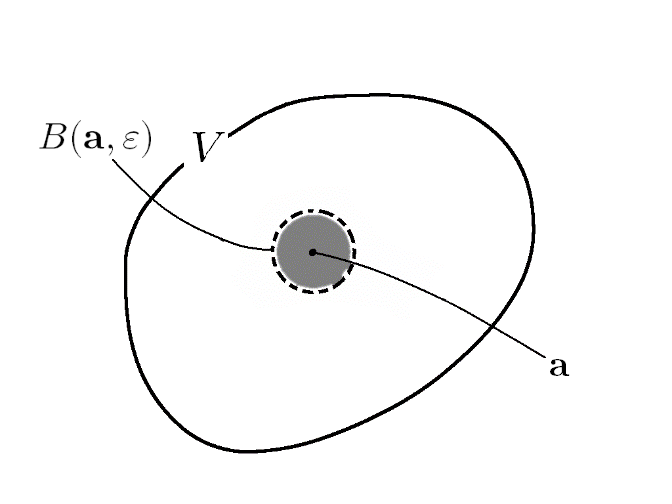
\includegraphics[width=60mm]{8.2.2.a.png}
\end{center}\par
ここで、特筆すべき$n$次元Euclid空間$E^{n}$の開基として次の定理たちのようなものがある。
\begin{thm}\label{8.2.2.3}
$n$次元Euclid空間$E^{n}$における位相空間$\left( \mathbb{R}^{n},\mathfrak{O}_{d_{E^{n}}} \right)$について、$\mathbf{a} \in \mathbb{R}^{n}$なる開球体$B\left( \mathbf{a},\varepsilon \right)$全体の集合$\mathfrak{B}$と、$\forall i \in \varLambda_{n}$に対し、$a_{i},b_{i} \in \mathbb{R}$が成り立つとき、直積$\prod_{i \in \varLambda_{n}} \left( a_{i},b_{i} \right)$全体の集合$\mathcal{I}$はどちらもその位相空間$\left( \mathbb{R}^{n},\mathfrak{O}_{d_{E^{n}}} \right)$の開基となる。
\end{thm}
\begin{proof}
$n$次元Euclid空間$E^{n}$における位相空間$\left( \mathbb{R}^{n},\mathfrak{O}_{d_{E^{n}}} \right)$について、$\mathbf{a} \in \mathbb{R}^{n}$なる開球$B\left( \mathbf{a},\varepsilon \right)$全体の集合$\mathfrak{B}$と、$\forall i \in \varLambda_{n}$に対し、$a_{i},b_{i} \in \mathbb{R}$が成り立つとき、直積$\prod_{i \in \varLambda_{n}} \left( a_{i},b_{i} \right)$全体の集合$\mathcal{I}$が与えられたとする。\par
このとき、$\forall O \in \mathfrak{O}_{d_{E^{n}}}\forall\mathbf{a} \in O$に対し、$\mathbf{a} = \left( a_{i} \right)_{i \in \varLambda_{n}}$とおくと、定義より明らかに$\mathbf{a} \in B\left( \mathbf{a},\varepsilon \right) \subseteq O$が成り立つような開球体$B\left( \mathbf{a},\varepsilon \right)$がその集合$\mathfrak{B}$に存在する。したがって、その集合$\mathfrak{B}$はその位相空間$\left( \mathbb{R}^{n},\mathfrak{O}_{d_{E^{n}}} \right)$の開基となる。\par
また、$\forall O \in \mathfrak{O}_{d_{E^{n}}}\forall\mathbf{a} \in O$に対し、定義より$\mathbf{a} \in B\left( \mathbf{a},\varepsilon \right) \subseteq O$が成り立つような開球体$B\left( \mathbf{a},\varepsilon \right)$が存在する。ここで、定理\ref{8.2.1.22}より次式が成り立つので、
\begin{align*}
\prod_{i \in \varLambda_{n}} {B\left( a_{i},\frac{\varepsilon}{\sqrt{n}} \right)} &= \prod_{i \in \varLambda_{n}} \left\{ b_{i} \in \mathbb{R} \middle| d_{E}\left( a_{i},b_{i} \right) < \frac{\varepsilon}{\sqrt{n}} \right\}\\
&= \prod_{i \in \varLambda_{n}} \left\{ b_{i} \in \mathbb{R} \middle| \left| a_{i} - b_{i} \right| < \frac{\varepsilon}{\sqrt{n}} \right\}\\
&= \prod_{i \in \varLambda_{n}} \left\{ b_{i} \in \mathbb{R} \middle| - \frac{\varepsilon}{\sqrt{n}} < a_{i} - b_{i} < \frac{\varepsilon}{\sqrt{n}} \right\}\\
&= \prod_{i \in \varLambda_{n}} \left\{ b_{i} \in \mathbb{R} \middle| a_{i} - \frac{\varepsilon}{\sqrt{n}} < b_{i} < a_{i} + \frac{\varepsilon}{\sqrt{n}} \right\}\\
&= \prod_{i \in \varLambda_{n}} \left( a_{i} - \frac{\varepsilon}{\sqrt{n}},a_{i} + \frac{\varepsilon}{\sqrt{n}} \right) \subseteq B\left( \mathbf{a},\varepsilon \right)
\end{align*}
$\forall O \in \mathfrak{O}_{d_{E^{n}}}\forall\mathbf{a} \in O\exists\prod_{i \in \varLambda_{n}} \left( a_{i} - \frac{\varepsilon}{\sqrt{n}},a_{i} + \frac{\varepsilon}{\sqrt{n}} \right)\in \mathcal{I}$に対し、$\mathbf{a} \in \prod_{i \in \varLambda_{n}} \left( a_{i} - \frac{\varepsilon}{\sqrt{n}},a_{i} + \frac{\varepsilon}{\sqrt{n}} \right) \subseteq O$が成り立ち、したがって、その集合$\mathcal{I}$はその位相空間$\left( \mathbb{R}^{n},\mathfrak{O}_{d_{E^{n}}} \right)$の開基となる。
\end{proof}
\begin{thm}\label{8.2.2.4}
さらに、$n$次元Euclid空間$E^{n}$における位相空間$\left( \mathbb{R}^{n},\mathfrak{O}_{d_{E^{n}}} \right)$について、$\mathbf{a}' \in \mathbb{R}^{n}$なる開球体$B\left( \mathbf{a}',r \right)$のうち、$\mathbf{a}' \in \mathbb{Q}^{n}$かつ$r \in \mathbb{Q}$を満たすもの全体の集合$\mathfrak{B}'$もまたその位相空間$\left( \mathbb{R}^{n},\mathfrak{O}_{d_{E^{n}}} \right)$の開基となる。
\end{thm}\par
これは次の図のように考えられることで示される。
\begin{center}
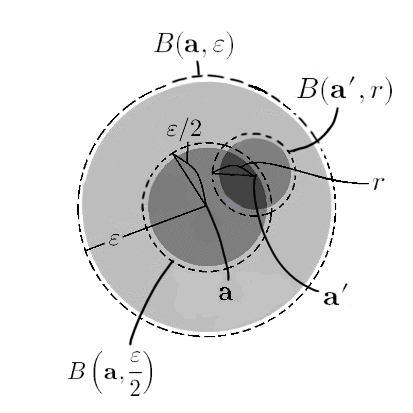
\includegraphics[width=60mm]{8.2.2.b.png}
\end{center}
\begin{proof}
$n$次元Euclid空間$E^{n}$における位相空間$\left( \mathbb{R}^{n},\mathfrak{O}_{d_{E^{n}}} \right)$について、$\mathbf{a}' \in \mathbb{R}^{n}$なる開球$B\left( \mathbf{a}',r \right)$のうち、$\mathbf{a}' \in \mathbb{Q}^{n}$かつ$r \in \mathbb{Q}$を満たすもの全体の集合$\mathfrak{B}'$が与えられたとする。\par
$\forall O \in \mathfrak{O}_{d_{E^{n}}}\forall\mathbf{a} \in O$に対し、定義より明らかに$\mathbf{a} \in B\left( \mathbf{a},\varepsilon \right) \subseteq O$が成り立つような開球体$B\left( \mathbf{a},\varepsilon \right)$がその集合$\mathfrak{B}$に存在する。ここで、開球体$B\left( \mathbf{a},\frac{\varepsilon}{2} \right)$の$\mathbf{a}' \in \mathbb{Q}^{n}$なる元$\mathbf{a}'$がとられ、さらに、有理数の稠密性より$d_{E^{n}}\left( \mathbf{a},\mathbf{a}' \right) < r < \frac{\varepsilon}{2}$なる有理数$r$もとられることができるで、$B\left( \mathbf{a}',r \right) \subseteq B\left( \mathbf{a},\varepsilon \right)$が成り立つ。これにより、$\forall O \in \mathfrak{O}_{d_{E^{n}}}\forall\mathbf{a} \in O\exists B\left( \mathbf{a}',\varepsilon \right) \in \mathfrak{B}'$に対し、$\mathbf{a} \in B\left( \mathbf{a}',r \right) \subseteq O$が成り立ち、したがって、その集合$\mathfrak{B}'$はその位相空間$\left( \mathbb{R}^{n},\mathfrak{O}_{d_{E^{n}}} \right)$の開基となる。
\end{proof}
\begin{thm}\label{8.2.2.5}
その位相空間$\left( \mathbb{R}^{n},\mathfrak{O}_{d_{E^{n}}} \right)$は第2可算公理を満たす。
\end{thm}
\begin{proof} 定理\ref{8.2.2.4}での開基$\mathfrak{B}'$を用いて${\#}\mathfrak{B}' = {\#}\left( \mathbb{Q}^{n} \times \mathbb{Q} \right) = \aleph_{0}$が成り立つことによる。
\end{proof}
%\hypertarget{euclidux7a7aux9593ux306bux304aux3051ux308bux4f4dux76f8ux7a7aux9593ux306eux9023ux7d9aux5199ux50cf}{%
\subsubsection{Euclid空間における位相空間の連続写像}%\label{euclidux7a7aux9593ux306bux304aux3051ux308bux4f4dux76f8ux7a7aux9593ux306eux9023ux7d9aux5199ux50cf}}
\begin{dfn}
ここで、詳しくは解析学のほうに参照してもらいたいが、1つの位相空間$\left( S,\mathfrak{O} \right)$が与えられ写像$f:S \rightarrow \mathbb{R}^{n}$がその位相空間$\left( S,\mathfrak{O} \right)$から$n$次元Euclid空間$E^{n}$における位相空間$\left( \mathbb{R}^{n},\mathfrak{O}_{d_{E^{n}}} \right)$への連続写像であるとき、その写像$f$は実連続関数であるともいう。
\end{dfn}
\begin{thm}\label{8.2.2.6}
ここで、1つの位相空間$\left( S,\mathfrak{O} \right)$が与えられ写像$f:S \rightarrow \mathbb{R}$について、次のことは同値である。
\begin{itemize}
\item
  その写像$f$がその位相空間$\left( S,\mathfrak{O} \right)$から1次元Euclid空間$E$における位相空間$\left( \mathbb{R},\mathfrak{O}_{d_{E}} \right)$への連続写像である。
\item
  $\forall a,b \in \mathbb{R}$に対し、開区間$(a,b)$に制限されたその逆対応$f^{- 1}$の値域$V\left( f^{- 1}|(a,b) \right)$がその位相$\mathfrak{O}$に属する。
\item
  $\forall c \in \mathbb{R}$に対し、開区間たち$(c,\infty)、( - \infty,c)$に制限されたその逆対応$f^{- 1}$の値域たち$V\left( f^{- 1}|(c,\infty) \right)$、$V\left( f^{- 1}|( - \infty,c) \right)$がその位相$\mathfrak{O}$に属する。
\end{itemize}
\end{thm}
\begin{proof}
1つの位相空間$\left( S,\mathfrak{O} \right)$が与えられ写像$f:S \rightarrow \mathbb{R}$について、その写像$f$がその位相空間$\left( S,\mathfrak{O} \right)$から1次元Euclid空間$E$における位相空間$\left( \mathbb{R},\mathfrak{O}_{d_{E}} \right)$への連続写像であるとする。このとき、開区間$(a,b)$全体の集合$\mathcal{I}$は定理\ref{8.2.2.3}よりその位相空間$\left( \mathbb{R},\mathfrak{O}_{d_{E}} \right)$の開基となり、したがって、準開基でもあるのであった。定理\ref{8.1.3.2}よりその写像$f:S \rightarrow \mathbb{R}$が連続であるならそのときに限り、$\forall I\in \mathcal{I}$に対し、$V\left( f^{- 1} \middle| I \right)\in \mathfrak{O}$が成り立つことになる、即ち、$\forall a,b \in \mathbb{R}$に対し、開区間$(a,b)$に制限されたその逆対応$f^{- 1}$の値域$V\left( f^{- 1}|(a,b) \right)$がその位相$\mathfrak{O}$に属することになる。\par
さらに、その集合$\mathfrak{U}$の任意の元は開区間で任意の開区間$(a,b)$は$(a,b) = (a,\infty) \cap ( - \infty,b)$のように書き換えられることができるので、定義より明らかに$c \in \mathbb{R}$なる開区間たち$(c,\infty)$、$( - \infty,c)$全体の集合$\mathcal{I}'$はその位相空間$\left( \mathbb{R},\mathfrak{O}_{d_{E}} \right)$の開基となり、したがって、準開基でもある。ここで、定理\ref{8.1.3.2}よりその写像$f:S \rightarrow \mathbb{R}$が連続であるならそのときに限り、$\forall I \in \mathcal{I}'$に対し、$V\left( f^{- 1} \middle| I \right)\in \mathfrak{O}$が成り立つことになる、即ち、$\forall c \in D$に対し、開区間たち$(c,\infty)$、$( - \infty,c)$に制限されたその逆対応$f^{- 1}$の値域たち$V\left( f^{- 1}|(c,\infty) \right)$、$V\left( f^{- 1}|( - \infty,c) \right)$がその位相$\mathfrak{O}$に属することになる。
\end{proof}
\begin{thm}\label{8.2.2.7}
1つの位相空間$\left( S,\mathfrak{O} \right)$と$n$次元Euclid空間$E^{n}$が与えられたとき、写像$f:S \rightarrow \mathbb{R}^{n}$が連続であるならそのときに限り、$\forall a \in S\forall\varepsilon \in \mathbb{R}^{+}$に対し、これのある近傍$V$をとれば、$\forall b \in V$に対し、$d_{E^{n}}\left( f(a),f(b) \right) < \varepsilon$が成り立つ。
\end{thm}\par
特に、その位相空間$\left( S,\mathfrak{O} \right)$が$m$次元Euclid空間$E^{m}$における位相空間であるなら、定理\ref{8.2.1.14}より$\forall\varepsilon \in \mathbb{R}^{+}\exists\delta \in \mathbb{R}^{+}\forall b \in \mathbb{R}^{m}$に対し、$d_{E^{m}}(a,b) < \delta$なら$d_{E^{n}}\left( f(a),f(b) \right) < \varepsilon$が成り立つ。この式はいわゆる$\varepsilon $-$\delta $論法の式である。
\begin{proof}
1つの位相空間$\left( S,\mathfrak{O} \right)$と$n$次元Euclid空間$E^{n}$が与えられたとき、$\forall\mathbf{a} \in \mathbb{R}^{n}$に対し、その元を中心とする開球体全体の集合$\mathfrak{U}_{\mathbf{a}}$は定理\ref{8.2.1.6}よりその元$\mathbf{a}$のその$n$次元Euclid空間における位相空間$\left( \mathbb{R}^{n},\mathfrak{O}_{d_{E^{n}}} \right)$における基本近傍系となり、したがって、全近傍系となるのであった。\par
ここで、定理\ref{8.1.3.1}より写像$f:S \rightarrow \mathbb{R}^{n}$が連続であるならそのときに限り、$a \in S$かつ$\mathbf{a} \in \mathbb{R}^{n}$なる元々$a$、$\mathbf{a}$のそれらの位相空間たち$\left( S,\mathfrak{O} \right)$、$\left( \mathbb{R}^{n},\mathfrak{O}_{d_{E^{n}}} \right)$の全近傍系たちがそれぞれ$\mathbf{V}(a)$、$\mathfrak{U}_{\mathbf{a}}$とおかれると、$B\left( f(a),\varepsilon \right) \in \mathfrak{U}_{f(a)}$なら$V\left( f^{- 1}|B\left( f(a),\varepsilon \right) \right) \in \mathbf{V}(a)$が成り立つ。ここで、$V\left( f^{- 1}|B\left( f(a),\varepsilon \right) \right) \in \mathbf{V}(a)$について、$B\left( f(a),\varepsilon \right) \in \mathfrak{U}_{f(a)}$が成り立つかつ、その写像$f$が連続であるので、$V\left( f^{- 1}|B\left( f(a),\varepsilon \right) \right)\in \mathfrak{O}$が成り立つことに注意すれば、次のようになる。
\begin{align*}
V\left( f^{- 1}|B\left( f(a),\varepsilon \right) \right) \in \mathbf{V}(a) &\Leftrightarrow a \in {\mathrm{int}}{V\left( f^{- 1}|B\left( f(a),\varepsilon \right) \right)}\\
&\Leftrightarrow a \in V\left( f^{- 1}|B\left( f(a),\varepsilon \right) \right)\\
&\Leftrightarrow a \in \left\{ b \in S \middle| \exists a' \in B\left( f(a),\varepsilon \right)\left[ f(b) = a' \right] \right\}\\
&\Leftrightarrow a \in \left\{ b \in S \middle| f(b) \in B\left( f(a),\varepsilon \right) \right\}\\
&\Leftrightarrow a \in \left\{ b \in S \middle| d_{E^{n}}\left( f(a),f(b) \right) < \varepsilon \right\}
\end{align*}
ここで、その値域$V\left( f^{- 1}|B\left( f(a),\varepsilon \right) \right)$を$V$とおくと、$\forall b \in V$に対し、次式が成り立つ。
\begin{align*}
d_{E^{n}}\left( f(a),f(b) \right) < \varepsilon
\end{align*}\par
以上より、その写像$f:S \rightarrow \mathbb{R}^{n}$が連続であるならそのときに限り、$\forall a \in S\forall\varepsilon \in \mathbb{R}^{+}$に対し、これのある近傍$V$をとれば、$\forall b \in V$に対し、$d_{E^{n}}\left( f(a),f(b) \right) < \varepsilon$が成り立つ。
\end{proof}
\begin{thm}\label{8.2.2.8}
1つの位相空間$\left( S,\mathfrak{O} \right)$と$n$次元Euclid空間$E^{n}$が与えられたとき、写像たち$f:S \rightarrow \mathbb{R}^{n}$、$g:S \rightarrow \mathbb{R}^{n}$が連続であるなら、$\forall a,b \in \mathbb{R}$に対し、その写像$af + bg$も連続で、特に、$n = 1$のとき、写像たち$fg$、$\frac{f}{g}$も連続である\footnote{実いうと、$n = 2$のとき、$\mathbb{C} =\mathbb{R}^2 $と考えれば、複素数の積の定義より複素数同士の積や商はそれぞれ実数の和積、和積と商で書かれることができるので、$n = 2$のときでも写像たち$fg$、$\frac{f}{g}$も連続となります。}。
\end{thm}
\begin{proof}
1つの位相空間$\left( S,\mathfrak{O} \right)$と$n$次元Euclid空間$E^{n}$が与えられたとき、写像たち$f:S \rightarrow \mathbb{R}^{n}$、$g:S \rightarrow \mathbb{R}^{n}$が連続であるなら、$\forall s \in S\forall\varepsilon \in \mathbb{R}^{+}$に対し、これのある近傍たち$V$、$W$をとれば、$\forall v \in V\forall w \in W$に対し、次式が成り立つ。
\begin{align*}
d_{E^{n}}\left( f(s),f(v) \right) < \varepsilon,\ \ d_{E^{n}}\left( g(s),g(w) \right) < \varepsilon
\end{align*}
特に、$\forall v \in V \cap W$に対し、次式が成り立つ。
\begin{align*}
d_{E^{n}}\left( f(s),f(v) \right) < \varepsilon,\ \ d_{E^{n}}\left( g(s),g(v) \right) < \varepsilon
\end{align*}
ここで、$\forall a,b \in \mathbb{R}$に対し、$a = b = 0$のときは明らかであるから、$a \neq 0$または$b \neq 0$のとき、次のようになる。
\begin{align*}
d_{E^{n}}\left( (af + bg)(s),(af + bg)(v) \right) &= d_{E^{n}}\left( af(s) + bg(s),af(v) + bg(v) \right)\\
&= d_{E^{n}}\left( af(s) - af(v),bg(s) - bg(v) \right)\\
&\leq d_{E^{n}}\left( af(s) - af(v),0 \right) + d_{E^{n}}\left( bg(s) - bg(v),0 \right)\\
&= d_{E^{n}}\left( af(s),af(v) \right) + d_{E^{n}}\left( bg(s),bg(v) \right)\\
&= |a|d_{E^{n}}\left( f(s),f(v) \right) + |b|d_{E^{n}}\left( g(s),g(v) \right)\\
&< |a|\varepsilon + |b|\varepsilon = \left( |a| + |b| \right)\varepsilon
\end{align*}
定理\ref{8.2.2.7}よりその写像$af + bg$も連続である。\par
特に、$n = 1$のとき、次のようになる。
\begin{align*}
d_{E}\left( fg(s),fg(v) \right) &= d_{E}\left( f(s)g(s),f(v)g(v) \right)\\
&= d_{E}\left( f(s)g(s) + f(s)g(v) - f(s)g(v),f(v)g(v) \right)\\
&= d_{E}\left( f(s)g(s) - f(s)g(v), - f(s)g(v) + f(v)g(v) \right)\\
&= d_{E}\left( f(s)\left( g(s) - g(v) \right), - g(v)\left( f(s) - f(v) \right) \right)\\
&\leq d_{E}\left( f(s)\left( g(s) - g(v) \right),0 \right) + d_{E}\left( - g(v)\left( f(s) - f(v) \right),0 \right)\\
&= d_{E}\left( f(s),0 \right)d_{E}\left( g(s) - g(v),0 \right) + d_{E}\left( g(v),0 \right)d_{E}\left( f(s) - f(v),0 \right)\\
&= d_{E}\left( f(s),0 \right)d_{E}\left( g(s),g(v) \right) + d_{E}\left( g(v),0 \right)d_{E}\left( f(s),f(v) \right)\\
&\leq \left( d_{E}\left( f(s),f(v) \right) + d_{E}\left( f(v),0 \right) \right)d_{E}\left( g(s),g(v) \right) + d_{E}\left( g(v),0 \right)d_{E}\left( f(s),f(v) \right)\\
&< \left( \varepsilon + d_{E}\left( f(v),0 \right) \right)\varepsilon + d_{E}\left( g(v),0 \right)\varepsilon\\
&= \left( \varepsilon + d_{E}\left( f(v),0 \right) + d_{E}\left( g(v),0 \right) \right)\varepsilon
\end{align*}
定理\ref{8.2.2.7}よりその写像$fg$も連続である。\par
また、$0 < \varepsilon < \frac{1}{2}d_{E}\left( g(v),0 \right)$とおかれれば、$d_{E}\left( g(s),g(v) \right) < \varepsilon < \frac{1}{2}d_{E}\left( g(v),0 \right)$が成り立ち、したがって、次のようになる。
\begin{align*}
\frac{1}{2}d_{E}\left( g(v),0 \right) &= d_{E}\left( g(v),0 \right) - \frac{1}{2}d_{E}\left( g(v),0 \right)\\
&< d_{E}\left( g(v),0 \right) - \varepsilon\\
&= d_{E}\left( g(v),0 \right) - d_{E}\left( g(s),0 \right) + d_{E}\left( g(s),0 \right) - \varepsilon\\
&\leq d_{E}\left( g(v),g(s) \right) + d_{E}\left( g(s),0 \right) - d_{E}\left( g(s),0 \right) + d_{E}\left( g(s),0 \right) - \varepsilon\\
&= d_{E}\left( g(v),g(s) \right) + d_{E}\left( g(s),0 \right) - \varepsilon\\
&< \varepsilon + d_{E}\left( g(s),0 \right) - \varepsilon\\
&= d_{E}\left( g(s),0 \right)
\end{align*}
これにより、次のようになる。
\begin{align*}
d_{E}\left( \frac{1}{g(s)},\frac{1}{g(v)} \right) &= d_{E}\left( \frac{1}{g(s)} - \frac{1}{g(v)},0 \right)\\
&= d_{E}\left( \frac{g(v) - g(s)}{g(s)g(v)},0 \right)\\
&= \frac{d_{E}\left( g(v) - g(s),0 \right)}{d_{E}\left( g(s),0 \right)d_{E}\left( g(v),0 \right)}\\
&= \frac{d_{E}\left( g(s),g(v) \right)}{d_{E}\left( g(s),0 \right)d_{E}\left( g(v),0 \right)}\\
&< \frac{\varepsilon}{\frac{1}{2}{d_{E}\left( g(v),0 \right)}^{2}}
\end{align*}
定理\ref{8.2.2.7}よりその写像$\frac{f}{g}$も連続である。
\end{proof}
\begin{thm}\label{8.2.2.9}
距離空間$(S,d)$が与えられたとき、その距離関数$d$がその距離空間$(S,d)$の直積距離空間$\left( S \times S,d' \right)$における位相空間$\left( S \times S,\mathfrak{O}_{d'} \right)$から1次元Euclid空間$E$における位相空間$\left( \mathbb{R},\mathfrak{O}_{d_{E}} \right)$への連続写像である。
\end{thm}
\begin{proof}
距離空間$(S,d)$が与えられたとき、直積$S \times S$の元の列$\left( a_{n},b_{n} \right)_{n \in \mathbb{N}}$が極限をもつとすれば、定理\ref{8.2.1.24}より次式が成り立つので、
\begin{align*}
\lim_{n \rightarrow \infty}{d\left( a_{n},b_{n} \right)} = d\left( \lim_{n \rightarrow \infty}a_{n},\lim_{n \rightarrow \infty}b_{n} \right)
\end{align*}
定理\ref{8.2.1.14}よりその距離関数$d$がその距離空間$(S,d)$の直積距離空間$\left( S \times S,d' \right)$における位相空間$\left( S \times S,\mathfrak{O}_{d'} \right)$から1次元Euclid空間$E$における位相空間$\left( \mathbb{R},\mathfrak{O}_{d_{E}} \right)$への連続写像である。
\end{proof}
\begin{thm}\label{8.2.2.10}
1次元Euclid空間$E$における位相空間$\left( \mathbb{R},\mathfrak{O}_{d_{E}} \right)$は、$\forall a,b \in \mathbb{R}$に対し、開区間$(a,b)$を台集合とする部分位相空間$\left( (a,b),\left( \mathfrak{O}_{d_{E}} \right)_{(a,b)} \right)$と同相である。
\end{thm}
\begin{proof}
1次元Euclid空間$E$における位相空間$\left( \mathbb{R},\mathfrak{O}_{d_{E}} \right)$について、$\forall a,b \in \mathbb{R}$に対し、開区間$(a,b)$を台集合とする部分位相空間$\left( (a,b),\left( \mathfrak{O}_{d_{E}} \right)_{(a,b)} \right)$が与えられたとき、次のような写像$f$が考えられれば、
\begin{align*}
f&:( - 1,1) \rightarrow \mathbb{R};x \mapsto \frac{x}{1 - x^{2}}\\
g&:(a,b) \rightarrow ( - 1,1);x \mapsto \frac{2}{b - a}\left( x - \frac{a + b}{2} \right)
\end{align*}
その合成写像$f \circ g$がこれらの位相空間たち$\left( \mathbb{R},\mathfrak{O}_{d_{E}} \right)$、$\left( (a,b),\left( \mathfrak{O}_{d_{E}} \right)_{(a,b)} \right)$の間の同相写像となる。
\end{proof}
%\hypertarget{euclidux7a7aux9593ux306bux304aux3051ux308bux4f4dux76f8ux7a7aux9593ux306eux9023ux7d50}{%
\subsubsection{Euclid空間における位相空間の連結}%\label{euclidux7a7aux9593ux306bux304aux3051ux308bux4f4dux76f8ux7a7aux9593ux306eux9023ux7d50}}
\begin{thm}\label{8.2.2.11}
1次元Euclid空間$E$における位相空間$\left( \mathbb{R},\mathfrak{O}_{d_{E}} \right)$について、$\forall a,b \in \mathbb{R}$に対し、次の集合たちを台集合とする部分位相空間はいづれも連結である。
\begin{align*}
\mathbb{R},\ \ (a,b),\ \ [ a,b]&,\ \ (a,b],\ \ [ a,b), \\ 
(a,\infty),\ \ [ a,\infty),\ \ &( - \infty,b),\ \ ( - \infty,b]
\end{align*}
\end{thm}
\begin{proof}
1次元Euclid空間$E$における位相空間$\left( \mathbb{R},\mathfrak{O}_{d_{E}} \right)$について、空集合でない2つの閉集合たち$A$、$B$を用いて$\mathbb{R} = A \sqcup B$が成り立つと仮定しよう。これらの閉集合たちの実数たちそれぞれ$a$、$b$がとられれば、$a \neq b$が成り立つので、$a < b$としても一般性は失われなくそうする。このとき、$a \in A \cap ( - \infty,b)$が成り立つので、$A \cap ( - \infty,b) \neq \emptyset$が成り立つ。また、その実数$b$がその集合$A \cap ( - \infty,b)$の1つの上界であるから、その集合$A \cap ( - \infty,b)$の上限$c$が存在して$c = \sup\left( A \cap ( - \infty,b) \right) \leq b$が成り立ち、したがって、$\forall\varepsilon \in \mathbb{R}^{+}$に対し、$c - \varepsilon < a' \leq c$なる実数$a'$がその集合$A \cap ( - \infty,b)$に、したがって、その集合$A$に存在するので、$(c - \varepsilon,c + \varepsilon) \cap A \neq \emptyset$が成り立つ、即ち、$B(c,\varepsilon) \cap A \neq \emptyset$が成り立つ。ここで、定理\ref{8.1.2.17}と定理\ref{8.2.1.9}より$c \in {\mathrm{cl}}A = A$が成り立つ。これにより、$c < b$が成り立つ。一方で、$c = \sup\left( A \cap ( - \infty,b) \right) < d \leq b$なる実数$d$が$d \in A$を満たすとすれば、$d \neq b$が成り立つので、$d \in A \cap ( - \infty,b)$が成り立つことになるが、これは上限の定義に矛盾している。したがって、$d \in \mathbb{R} \setminus A = B$が成り立つ。このとき、$\forall\varepsilon \in \mathbb{R}^{+}$に対し、$d \in (c - \varepsilon,c + \varepsilon)$が成り立つので、$(c - \varepsilon,c + \varepsilon) \cap B \neq \emptyset$が成り立つ、即ち、$B(c,\varepsilon) \cap B \neq \emptyset$が成り立つ。ここで、定理\ref{8.1.2.17}と定理\ref{8.2.1.9}より$c \in {\mathrm{cl}}B = B$が成り立つ。これにより、$c \in A \cap B$が成り立つことになるが、これは仮定に矛盾している。したがって、空集合でない任意の2つの閉集合たち$A$、$B$は$\mathbb{R} = A \sqcup B$を満たせない。したがって、定理\ref{8.1.5.1}より1次元Euclid空間$E$における位相空間$\left( \mathbb{R},\mathfrak{O}_{d_{E}} \right)$は連結である。\par
また、$\forall a,b \in \mathbb{R}$に対し、その部分位相空間$\left( (a,b),\left( \mathfrak{O}_{d_{E}} \right)_{(a,b)} \right)$は定理\ref{8.2.2.10}より連結である。さらに、定理\ref{8.1.5.5}より$\forall a,b \in \mathbb{R}$に対し、次の集合たちを台集合とする部分位相空間はいづれも連結である。
\begin{align*}
[ a,b],\ \ (a,b],\ \ [ a,b)
\end{align*}
最後に、定理\ref{8.1.5.7}より$\forall a,b \in \mathbb{R}$に対し、次式のようにおかれれば、
\begin{align*}
(a,\infty) = \bigcup_{n \in \mathbb{N}} (a,a + n)&,\ \ [ a,\infty) = \bigcup_{n \in \mathbb{N}} [ a,a + n),\\ 
( - \infty,b) = \bigcup_{n \in \mathbb{N}} (b - n,b)&,\ \ ( - \infty,b] = \bigcup_{n \in \mathbb{N}} (b - n,b]
\end{align*}
次の集合たちを台集合とする部分位相空間はいづれも連結である。
\begin{align*}
(a,\infty),\ \ [ a,\infty),\ \ ( - \infty,b),\ \ ( - \infty,b]
\end{align*}\par
以上、$\forall a,b \in \mathbb{R}$に対し、上記の集合たちを台集合とする部分位相空間はいづれも連結であることが示された。
\end{proof}
\begin{thm}\label{8.2.2.12}
$n$次元Euclid空間$E^{n}$における位相空間$\left( \mathbb{R}^{n},\mathfrak{O}_{d_{E^{n}}} \right)$は連結である。
\end{thm}
\begin{proof} 定理\ref{8.1.5.11}と定理\ref{8.2.2.11}より明らかである。
\end{proof}
\begin{thm}\label{8.2.2.13}
1次元Euclid空間$E$における位相空間$\left( \mathbb{R},\mathfrak{O}_{d_{E}} \right)$の連結な部分位相空間$\left( M,\mathfrak{O}_{M} \right)$が与えられたとき、$\forall a,b \in M$に対し、$a < b$が成り立つなら、$[ a,b] \subseteq M$が成り立つ。
\end{thm}
\begin{proof}
1次元Euclid空間$E$における位相空間$\left( \mathbb{R},\mathfrak{O}_{d_{E}} \right)$の連結な部分位相空間$\left( M,\mathfrak{O}_{M} \right)$が与えられたとする。$M = \left\{ a \right\}$が成り立つなら、$M = [ a,a]$が成り立つので、その部分集合$M$はこれの元を2つ以上もつとしてもよい。ここで、$\exists a,b \in M$に対し、$a < b$が成り立つかつ、$[ a,b] \subseteq M$が成り立たないと仮定する。このとき、$\exists c \in [ a,b]$に対し、$c \notin M$が成り立ち、したがって、次式が成り立つ。
\begin{align*}
M = M \setminus \left\{ c \right\} \subseteq \mathbb{R} \setminus \left\{ c \right\} = ( - \infty,c) \cup (c,\infty),\ \ ( - \infty,c) \cap (c,\infty) \cap M \subseteq ( - \infty,c) \cap (c,\infty) = \emptyset
\end{align*}
さらに、$a,b \in M$かつ$a \in ( - \infty,c)$かつ$b \in (c,\infty)$が成り立つので、$( - \infty,c) \cap M \neq \emptyset$かつ$(c,\infty) \cap M \neq \emptyset$が成り立つ。このとき、集合たち$( - \infty,c)$、$(c,\infty)$はいづれも開集合であり、次式が成り立つ。
\begin{align*}
M \subseteq ( - \infty,c) \cup (c,\infty)&,\ \ ( - \infty,c) \cap (c,\infty) \cap M = \emptyset,\\
( - \infty,c) \cap M \neq \emptyset&,\ \ (c,\infty) \cap M \neq \emptyset
\end{align*}
ここで、定理\ref{8.1.5.2}よりその位相空間$\left( \mathbb{R},\mathfrak{O}_{d_{E}} \right)$が連結でないことになるが、これは仮定に矛盾している。したがって、$\forall a,b \in M$に対し、$a < b$が成り立つなら、$[ a,b] \subseteq M$が成り立つ。
\end{proof}
\begin{thm}\label{8.2.2.14}
1次元Euclid空間$E$における位相空間$\left( \mathbb{R},\mathfrak{O}_{d_{E}} \right)$について、$\forall a,b \in \mathbb{R}$に対し、次の集合たちを台集合とする部分位相空間以外で連結な部分位相空間は存在しない。
\begin{align*}
\mathbb{R},\ \ (a,b),\ \ [ a,b]&,\ \ (a,b],\ \ [ a,b),\\ 
(a,\infty),\ \ [ a,\infty),\ \ &( - \infty,b),\ \ ( - \infty,b]
\end{align*}
\end{thm}
\begin{proof}
1次元Euclid空間$E$における位相空間$\left( \mathbb{R},\mathfrak{O}_{d_{E}} \right)$の連結な部分位相空間$\left( M,\mathfrak{O}_{M} \right)$が与えられたとする。定理\ref{8.2.2.13}より$\forall a,b \in M$に対し、$a < b$が成り立つなら、$[ a,b] \subseteq M$が成り立つ。\par
ここで、その部分集合が有界であるなら、上限性質より下限$\inf M$、上限$\sup M$が存在して、$M \subseteq \left[ \inf M,\sup M \right]$が成り立つ。ここで、$\forall a \in \left( \inf M,\sup M \right)$に対し、$a \notin M$が成り立つとすれば、$\forall b \in M$に対し、$a < b$または$b < a$が成り立ち、したがって、$a \leq \inf M \leq b$または$b \leq \sup M \leq a$が成り立つことになるが、これは$\inf M < a < \sup M$が成り立つことに矛盾する。したがって、$\left( \inf M,\sup M \right) \subseteq M$が成り立つことになる。これにより、その部分集合$M$は次のうちいづれかである。
\begin{align*}
\left( \inf M,\sup M \right),\ \ \left[ \inf M,\sup M \right],\ \ \left( \inf M,\sup M \right],\ \ \left[ \inf M,\sup M \right)
\end{align*}\par
その部分集合$M$が有限でなければ、その部分集合$M$は次のうちいづれかである。
\begin{align*}
\mathbb{R},\ \ \left( \inf M,\infty \right),\ \ \left[ \inf M,\infty \right),\ \ \left( - \infty,\sup M \right),\ \ \left( - \infty,\sup M \right]
\end{align*}\par
以上、$\forall a,b \in \mathbb{R}$に対し、上記の集合たちを台集合とする部分位相空間以外で連結な部分位相空間は存在しないことが示された。
\end{proof}
\begin{thm}\label{8.2.2.15}
1次元Euclid空間$E$における位相空間$\left( \mathbb{R},\mathfrak{O}_{d_{E}} \right)$について、$\forall a,b \in \mathbb{R}$に対し、次の集合たちを台集合とする部分位相空間以外で同相な部分位相空間は存在しない。
\begin{align*}
\mathbb{R},\ \ (a,b),\ \ (a,\infty),\ \ ( - \infty,b)
\end{align*}
\end{thm}
\begin{proof}
1次元Euclid空間$E$における位相空間$\left( \mathbb{R},\mathfrak{O}_{d_{E}} \right)$からこれの部分位相空間$\left( M,\mathfrak{O}_{M} \right)$への同相写像$f:\mathbb{R} \rightarrow M$が与えられたとき、その写像$f$はその位相空間$\left( \mathbb{R},\mathfrak{O}_{d_{E}} \right)$からその部分位相空間$\left( M,\mathfrak{O}_{M} \right)$へ連続写像でもあるから、定理\ref{8.1.5.3}よりその部分位相空間$\left( M,\mathfrak{O}_{M} \right)$は連結であり、定理\ref{8.2.2.14}より$\forall a,b \in \mathbb{R}$に対し、次の集合たちを台集合とする部分位相空間以外で連結な部分位相空間は存在しないのであった。
\begin{align*}
\mathbb{R},\ \ (a,b),\ \ [ a,b]&,\ \ (a,b],\ \ [ a,b),\\ 
(a,\infty),\ \ [ a,\infty),\ \ &( - \infty,b),\ \ ( - \infty,b]
\end{align*}
ここで、その写像$f$は同相写像なので、$V(f) = M$が成り立ち、開写像でもあるから、その部分集合$M$が開集合である。したがって、$\forall a,b \in \mathbb{R}$に対し、次の集合たちを台集合とする部分位相空間以外で同相な部分位相空間は存在しない。
\begin{align*}
\mathbb{R},\ \ (a,b),\ \ (a,\infty),\ \ ( - \infty,b)
\end{align*}
\end{proof}
\begin{thm}[中間値の定理の拡張]\label{8.2.2.16}
連結な位相空間$\left( S,\mathfrak{O} \right)$から1次元Euclid空間$E$における位相空間$\left( \mathbb{R},\mathfrak{O}_{d_{E}} \right)$への連続写像$f:S \rightarrow \mathbb{R}$について、$\forall a,b \in S$に対し、$f(a) < f(b)$が成り立つなら、$\forall\gamma \in \left[ f(a),f(b) \right]$に対し、$f(c) = \gamma$なるその集合$S$の元$c$が存在する。この定理を一般化された中間値の定理、中間値の定理の拡張ということにする。
\end{thm}
\begin{proof}
連結な位相空間$\left( S,\mathfrak{O} \right)$から1次元Euclid空間$E$における位相空間$\left( \mathbb{R},\mathfrak{O}_{d_{E}} \right)$への連続写像$f:S \rightarrow \mathbb{R}$について、定理\ref{8.1.5.3}よりその部分位相空間$\left( V(f),\mathfrak{O}_{V(f)} \right)$も連結であり、したがって、定理\ref{8.2.2.13}より$\forall\alpha,\beta \in V(f)$に対し、$\alpha < \beta$が成り立つなら、$[\alpha,\beta] \subseteq V(f)$が成り立つので、$\forall a,b \in S$に対し、$f(a) < f(b)$が成り立つなら、$\left[ f(a),f(b) \right] \subseteq V(f)$も成り立つ。したがって、$\forall\gamma \in \left[ f(a),f(b) \right]$に対し、$\gamma \in V(f)$が成り立つので、$f(c) = \gamma$なるその集合$S$の元$c$が存在する。
\end{proof}
%\hypertarget{ux5f27ux72b6ux9023ux7d50}{%
\subsubsection{弧状連結}%\label{ux5f27ux72b6ux9023ux7d50}}
\begin{dfn}
1次元Euclid空間$E$における位相空間$\left( \mathbb{R},\mathfrak{O}_{d_{E}} \right)$の部分位相空間$\left( [ 0,1],\left( \mathfrak{O}_{d_{E}} \right)_{[ 0,1]} \right)$から位相空間$\left( S,\mathfrak{O} \right)$への連続写像$f:[ 0,1] \rightarrow S$が与えられたとき、その写像$f$の値域$V(f)$をその位相空間$\left( S,\mathfrak{O} \right)$におけるその写像$f$による弧といい、その弧はその元$f(0)$とその元$f(1)$とを結ぶという。
\end{dfn}
\begin{thm}\label{8.2.2.17}
位相空間$\left( S,\mathfrak{O} \right)$における弧$A$を台集合とするその部分位相空間$\left( A,\mathfrak{O}_{A} \right)$は連結である。
\end{thm}
\begin{proof}
位相空間$\left( S,\mathfrak{O} \right)$における弧$A$を台集合とするその部分位相空間$\left( A,\mathfrak{O}_{A} \right)$が与えられたとき、1次元Euclid空間$E$における位相空間$\left( \mathbb{R},\mathfrak{O}_{d_{E}} \right)$の部分位相空間$\left( [ 0,1],\left( \mathfrak{O}_{d_{E}} \right)_{[ 0,1]} \right)$から位相空間$\left( S,\mathfrak{O} \right)$へのある連続写像$f:[ 0,1] \rightarrow S$が存在して$A = V(f)$が成り立つ。ここで、定理\ref{8.2.2.11}よりその部分位相空間$\left( [ 0,1],\left( \mathfrak{O}_{d_{E}} \right)_{[ 0,1]} \right)$は連結であり、定理\ref{8.1.5.3}よりその部分位相空間$\left( A,\mathfrak{O}_{A} \right)$も連結である。
\end{proof}
\begin{thm}\label{8.2.2.18}
$i \in \varLambda_{n}$なる位相空間$\left( S,\mathfrak{O} \right)$における連続写像たち$f_{i}$による弧々$A_{i}$が、$\forall i \in \varLambda_{n - 1}$に対し、$f_{i}(1) = f_{i + 1}(0)$を満たすなら、その和集合$\bigcup_{i \in \varLambda_{n}} A_{i}$もその元$f_{1}(0)$からその元$f_{n}(1)$への弧となる。
\end{thm}
\begin{proof}
$i \in \varLambda_{n}$なる位相空間$\left( S,\mathfrak{O} \right)$における写像たち$f_{i}$による弧々$A_{i}$が、$\forall i \in \varLambda_{n - 1}$に対し、$f_{i}(1) = f_{i + 1}(0)$を満たすとするなら、1次元Euclid空間$E$における位相空間$\left( \mathbb{R},\mathfrak{O}_{d_{E}} \right)$の部分位相空間$\left( [ 0,1],\left( \mathfrak{O}_{d_{E}} \right)_{[ 0,1]} \right)$からその位相空間$\left( S,\mathfrak{O} \right)$への写像$f:[ 0,1] \rightarrow S$が、$\bigcup_{i \in \varLambda_{n}} \left[ \frac{i - 1}{n},\frac{i}{n} \right] = [ 0,1]$が成り立つことにより、$\forall i \in \varLambda_{n}$に対し、$t \in \left[ \frac{i - 1}{n},\frac{i}{n} \right]$が成り立つなら、$f(t) = f_{i}(nt - i + 1)$が成り立つように定義されればよい。その写像$f$が連続であることは定理\ref{8.2.1.14}から直ちに分かる。
\end{proof}
\begin{dfn}
位相空間$\left( S,\mathfrak{O} \right)$が与えられたとき、$\forall a,b \in S$に対し、その元$a$とその元$b$を結ぶ弧$A$が存在するとき、その位相空間$\left( S,\mathfrak{O} \right)$は弧状連結であるという。
\end{dfn}
\begin{thm}\label{8.2.2.19}
弧状連結な位相空間$\left( S,\mathfrak{O} \right)$は連結である。\par
ただし、逆は必ずしも成り立つとは限らないことに注意されたい。
\end{thm}
\begin{proof}
弧状連結な位相空間$\left( S,\mathfrak{O} \right)$が与えられたとき、$\forall a,b \in S$に対し、その元$a$とその元$b$を結ぶ弧$A_{b}$が存在することになり、定理\ref{8.2.2.17}より、位相空間$\left( S,\mathfrak{O} \right)$における弧$A_{b}$を台集合とするその部分位相空間$\left( A_{b},\mathfrak{O}_{A_{b}} \right)$は連結である。さらに、$\forall b \in S$に対し、$a \in A_{b}$が成り立つので、定理\ref{8.1.5.7}よりその部分位相空間$\left( \bigcup_{b \in S} A_{b},\mathfrak{O}_{\bigcup_{b \in S} A_{b}} \right)$も連結である。ここで、明らかに$\bigcup_{b \in S} A_{b} \subseteq S$が成り立ち、$\forall b \in S$に対し、その位相空間$\left( S,\mathfrak{O} \right)$が弧状連結であるから、その元$a$とその元$b$とを結ぶ弧$A_{b}$が存在して$b \in A_{b}$が成り立ち、したがって、$b \in \bigcup_{b \in S} A_{b}$が成り立つので、$\bigcup_{b \in S} A_{b} = S$が成り立つ。これにより、連結なその部分位相空間$\left( \bigcup_{b \in S} A_{b},\mathfrak{O}_{\bigcup_{b \in S} A_{b}} \right)$はその位相空間$\left( S,\mathfrak{O} \right)$でもあるので、その位相空間$\left( S,\mathfrak{O} \right)$は連結である。
\end{proof}
%\hypertarget{ux51f8ux96c6ux5408}{%
\subsubsection{凸集合}%\label{ux51f8ux96c6ux5408}}
\begin{dfn}
$n$次元数空間$\mathbb{R}^{n}$の2点$\mathbf{a}$、$\mathbf{b}$に対し、次式のように定義される集合$l\left( \mathbf{a},\mathbf{b} \right)$をこれらの2点$\mathbf{a}$、$\mathbf{b}$を結ぶ線分という。
\begin{align*}
l\left( \mathbf{a},\mathbf{b} \right) = \left\{ \mathbf{l} \in \mathbb{R}^{n} \middle| \mathbf{l} = (1 - t)\mathbf{a} + t\mathbf{b},\ \ t \in [ 0,1] \right\}
\end{align*}
\end{dfn}
\begin{thm}\label{8.2.2.20}
$\forall\mathbf{a},\mathbf{b} \in \mathbb{R}^{n}$に対し、次式のように定義される写像$f$は1次元Euclid空間$E$における位相空間$\left( \mathbb{R},\mathfrak{O}_{d_{E}} \right)$の部分位相空間$\left( [ 0,1],\left( \mathfrak{O}_{d_{E}} \right)_{[ 0,1]} \right)$から$n$次元Euclid空間における位相空間$\left( \mathbb{R}^{n},\mathfrak{O}_{d_{E^{n}}} \right)$への連続写像$f:[ 0,1] \rightarrow \mathbb{R}^{n}$で、
\begin{align*}
f:[ 0,1] \rightarrow \mathbb{R}^{n};t \mapsto (1 - t)\mathbf{a} + t\mathbf{b}
\end{align*}
さらに、これらの2点$\mathbf{a}$、$\mathbf{b}$を結ぶ線分$l\left( \mathbf{a},\mathbf{b} \right)$はその写像$f$によるこれらの2点$\mathbf{a}$、$\mathbf{b}$を結ぶ弧である。
\end{thm}
\begin{proof} 定理\ref{8.2.1.14}より明らかである。
\end{proof}
\begin{dfn}
$n$次元数空間$\mathbb{R}^{n}$の部分集合$M$が与えられたとき、$\forall\mathbf{a},\mathbf{b} \in M$に対し、これらの線分$l\left( \mathbf{a},\mathbf{b} \right)$が$l\left( \mathbf{a},\mathbf{b} \right) \subseteq M$を満たすとき、その集合$M$は凸集合であるという。もちろん、$n$次元数空間$\mathbb{R}^{n}$自身も凸集合である。また、空集合も凸集合であるとする。
\end{dfn}
\begin{thm}\label{8.2.2.21}
$n$次元数空間$\mathbb{R}^{n}$の凸集合である部分集合$M$が与えられたとき、$n$次元Euclid空間における位相空間$\left( \mathbb{R}^{n},\mathfrak{O}_{d_{E^{n}}} \right)$の部分位相空間$\left( M,\left( \mathfrak{O}_{d_{E^{n}}} \right)_{M} \right)$は弧状連結である。
\end{thm}
\begin{proof}
$n$次元数空間$\mathbb{R}^{n}$の凸集合である部分集合$M$が与えられたとき、$n$次元Euclid空間における位相空間$\left( \mathbb{R}^{n},\mathfrak{O}_{d_{E^{n}}} \right)$の部分位相空間$\left( M,\left( \mathfrak{O}_{d_{E^{n}}} \right)_{M} \right)$について、$\forall\mathbf{a},\mathbf{b} \in M$に対し、これらの線分$l\left( \mathbf{a},\mathbf{b} \right)$は定理\ref{8.2.1.18}、定理\ref{8.2.2.20}よりこれらの2点$\mathbf{a}$、$\mathbf{b}$を結ぶ弧である。ゆえに、その部分位相空間$\left( M,\left( \mathfrak{O}_{d_{E^{n}}} \right)_{M} \right)$は弧状連結である。
\end{proof}
\begin{thm}\label{8.2.2.22}
$n$次元Euclid空間$E^{n}$における位相空間$\left( \mathbb{R}^{n},\mathfrak{O}_{d_{E^{n}}} \right)$の任意の元$\mathbf{a}$における任意の開球体$B\left( \mathbf{a},\varepsilon \right)$は凸集合である。
\end{thm}
\begin{proof}
$n$次元Euclid空間$E^{n}$における位相空間$\left( \mathbb{R}^{n},\mathfrak{O}_{d_{E^{n}}} \right)$の任意の元$\mathbf{a}$における任意の開球体$B\left( \mathbf{a},\varepsilon \right)$において、$\forall\mathbf{b},\mathbf{c} \in B\left( \mathbf{a},\varepsilon \right)$に対し、次式が成り立つ。
\begin{align*}
d_{E^{n}}\left( \mathbf{a},\mathbf{b} \right) < \varepsilon,\ \ d_{E^{n}}\left( \mathbf{a},\mathbf{c} \right) < \varepsilon
\end{align*}
ここで、これらの線分$l\left( \mathbf{b},\mathbf{c} \right)$の任意の元$\mathbf{l}$は、$\exists t \in [ 0,1]$に対し、$\mathbf{l} = (1 - t)\mathbf{b} + t\mathbf{c}$を満たすので、次のようになる。
\begin{align*}
d_{E^{n}}\left( \mathbf{a},\mathbf{l} \right) &= d_{E^{n}}\left( \mathbf{a},(1 - t)\mathbf{b} + t\mathbf{c} \right)\\
&= d_{E^{n}}\left( (1 - t)\mathbf{a} + t\mathbf{a},(1 - t)\mathbf{b} + t\mathbf{c} \right)\\
&= d_{E^{n}}\left( (1 - t)\mathbf{a} - (1 - t)\mathbf{b},t\mathbf{a} - t\mathbf{c} \right)\\
&\leq d_{E^{n}}\left( (1 - t)\mathbf{a} - (1 - t)\mathbf{b},\mathbf{0} \right) + d_{E^{n}}\left( t\mathbf{a} - t\mathbf{c},\mathbf{0} \right)\\
&= (1 - t)d_{E^{n}}\left( \mathbf{a},\mathbf{b} \right) + td_{E^{n}}\left( \mathbf{a},\mathbf{c} \right)\\
&< (1 - t)\varepsilon + t\varepsilon = \varepsilon
\end{align*}
これにより、$\mathbf{l} \in B\left( \mathbf{a},\varepsilon \right)$が成り立つので、$l\left( \mathbf{b},\mathbf{c} \right) \subseteq B\left( \mathbf{a},\varepsilon \right)$が成り立ち、したがって、その開球体$B\left( \mathbf{a},\varepsilon \right)$は凸集合である。
\end{proof}
%\hypertarget{ux9023ux7d50ux3068ux5f27ux72b6ux9023ux7d50}{%
\subsubsection{連結と弧状連結}%\label{ux9023ux7d50ux3068ux5f27ux72b6ux9023ux7d50}}
\begin{dfn} 定理\ref{8.2.2.20}より$i \in \varLambda_{m + 1}$なる$n$次元数空間$\mathbb{R}^{n}$の点々$\mathbf{a}_{i}$が与えられたとき、これらの点々を結ぶ線分$l\left( \mathbf{a}_{i},\mathbf{a}_{i + 1} \right)$が$n$次元Euclid空間における位相空間$\left( \mathbb{R}^{n},\mathfrak{O}_{d_{E^{n}}} \right)$における連続写像$f_{i}$による弧$L_{i}$とみなされることができるので、そうするとき、1次元Euclid空間$E$における位相空間$\left( \mathbb{R},\mathfrak{O}_{d_{E}} \right)$の部分位相空間$\left( [ 0,1],\left( \mathfrak{O}_{d_{E}} \right)_{[ 0,1]} \right)$からその位相空間$\left( \mathbb{R}^{n},\mathfrak{O}_{d_{E^{n}}} \right)$への写像$f:[ 0,1] \rightarrow \mathbb{R}^{n}$が、$\forall i \in \varLambda_{n}$に対し、$t \in \left[ \frac{i - 1}{n},\frac{i}{n} \right]$が成り立つなら、$f(t) = f_{i}(nt - i + 1)$が成り立つように定義されたとき、その写像$f$によるこれらの点々$\mathbf{a}_{1}$、$\mathbf{a}_{m + 1}$を結ぶ弧$L$をこれらの点々$\mathbf{a}_{1}$、$\mathbf{a}_{m + 1}$を結ぶ折線という。
\end{dfn}
\begin{thm}\label{8.2.2.23}
$n$次元Euclid空間$E^{n}$における位相空間$\left( \mathbb{R}^{n},\mathfrak{O}_{d_{E^{n}}} \right)$の開集合$O$を台集合とする部分位相空間$\left( O,\left( \mathfrak{O}_{d_{E^{n}}} \right)_{O} \right)$が連結であるなら、$\forall\mathbf{a},\mathbf{b} \in O$に対し、これらの点々とを結ぶ折線が存在する。
\end{thm}
\begin{proof}
$n$次元Euclid空間$E^{n}$における位相空間$\left( \mathbb{R}^{n},\mathfrak{O}_{d_{E^{n}}} \right)$の開集合$O$を台集合とする部分位相空間$\left( O,\left( \mathfrak{O}_{d_{E^{n}}} \right)_{O} \right)$が連結であるとする。$\forall\mathbf{a} \in O$に対し、これと折線で結べるその開集合$O$の元々全体を$A$、これと折線で結べないその開集合$O$の元々全体を$B$とおくと、$\mathbf{a} \in A$が成り立つので、$A \neq \emptyset$が成り立つ。また、もちろん$O = A \sqcup B$が成り立つ。\par
$\forall\mathbf{c} \in A$に対し、これらの点々$\mathbf{a}$、$\mathbf{c}$を結ぶ折線$L$が存在する。ここで、その集合$O$は開集合なので、ある開球体$B\left( \mathbf{c},\varepsilon \right)$が存在して$B\left( \mathbf{c},\varepsilon \right) \subseteq O$が成り立つ。$\forall\mathbf{c}' \in B\left( \mathbf{c},\varepsilon \right)$に対し、定理\ref{8.2.2.22}よりこれらの点々$\mathbf{c}$、$\mathbf{c}'$を結ぶ線分$l\left( \mathbf{c},\mathbf{c}' \right)$が$l\left( \mathbf{c},\mathbf{c}' \right) \subseteq B\left( \mathbf{c},\varepsilon \right)$を満たすので、その線分$l\left( \mathbf{c},\mathbf{c}' \right)$が$M$とおかれると、定理\ref{8.2.2.18}より集合$L \cup M$はこれらの点々$\mathbf{a}$、$\mathbf{c}'$を結ぶ折線となる。したがって、$\mathbf{c}' \in A$が成り立つので、$B\left( \mathbf{c},\varepsilon \right) \subseteq A$が成り立ち、したがって、その集合$A$は開集合である。\par
$\forall\mathbf{c} \in B$に対し、その集合$O$は開集合なので、ある開球体$B\left( \mathbf{c},\varepsilon \right)$が存在して$B\left( \mathbf{c},\varepsilon \right) \subseteq O$が成り立つ。$\forall\mathbf{c}' \in B\left( \mathbf{c},\varepsilon \right)$に対し、定理\ref{8.2.2.22}よりこれらの点々$\mathbf{c}$、$\mathbf{c}'$を結ぶ線分$l\left( \mathbf{c},\mathbf{c}' \right)$が$l\left( \mathbf{c},\mathbf{c}' \right) \subseteq B\left( \mathbf{c},\varepsilon \right)$を満たすので、その線分$l\left( \mathbf{c},\mathbf{c}' \right)$が$M$とおかれるとする。ここで、その元$\mathbf{c}'$とその元$\mathbf{a}$とを結ぶ折線$L$が存在するとすれば、定理\ref{8.2.2.18}より集合$L \cup M$はこれらの点々$\mathbf{a}$、$\mathbf{c}$を結ぶ折線となるが、これは$\mathbf{c} \in B$が成り立つことに矛盾する。したがって、$\mathbf{c}' \in B$が成り立つので、$B\left( \mathbf{c},\varepsilon \right) \subseteq B$が成り立ち、したがって、その集合$B$も開集合である。\par
以上の議論により、$O = A \sqcup B$かつ$A \neq \emptyset$かつこれらの集合たち$A$、$B$が開集合であり、その部分位相空間$\left( O,\left( \mathfrak{O}_{d_{E^{n}}} \right)_{O} \right)$が連結であるので、定理\ref{8.1.5.2}より$B = \emptyset$が成り立つ。よって、その部分位相空間$\left( O,\left( \mathfrak{O}_{d_{E^{n}}} \right)_{O} \right)$が連結であるなら、$\forall\mathbf{a},\mathbf{b} \in O$に対し、これらの点々を結ぶ折線が存在する。
\end{proof}
\begin{thm}\label{8.2.2.24}
$n$次元Euclid空間$E^{n}$における位相空間$\left( \mathbb{R}^{n},\mathfrak{O}_{d_{E^{n}}} \right)$の開集合$O$を台集合とする部分位相空間$\left( O,\left( \mathfrak{O}_{d_{E^{n}}} \right)_{O} \right)$について、次のことは同値である。
\begin{itemize}
\item
  その部分位相空間$\left( O,\left( \mathfrak{O}_{d_{E^{n}}} \right)_{O} \right)$が連結である。
\item
  $\forall\mathbf{a},\mathbf{b} \in O$に対し、これらの点々を結ぶ折線が存在する。
\item
  $\forall\mathbf{a},\mathbf{b} \in O$に対し、これらの点々を結ぶ弧が存在する。
\end{itemize}
\end{thm}
\begin{proof}
$n$次元Euclid空間$E^{n}$における位相空間$\left( \mathbb{R}^{n},\mathfrak{O}_{d_{E^{n}}} \right)$の開集合$O$を台集合とする部分位相空間$\left( O,\left( \mathfrak{O}_{d_{E^{n}}} \right)_{O} \right)$について、その部分位相空間$\left( O,\left( \mathfrak{O}_{d_{E^{n}}} \right)_{O} \right)$が連結であるなら、定理\ref{8.2.2.23}より$\forall\mathbf{a},\mathbf{b} \in O$に対し、これらの点々とを結ぶ折線が存在する。これが成り立つなら、明らかに$\forall\mathbf{a},\mathbf{b} \in O$に対し、これらの点々を結ぶ弧が存在する。これが成り立つなら、定理\ref{8.2.2.19}よりその部分位相空間$\left( O,\left( \mathfrak{O}_{d_{E^{n}}} \right)_{O} \right)$は連結である。\par
以上で示すべきことが示された。
\end{proof}
\begin{thm}\label{8.2.2.25}
添数集合$\varLambda$によって添数づけられた$n$次元数空間$\mathbb{R}^{n}$の凸集合である部分集合の族$\left\{ M_{\lambda} \right\}_{\lambda \in \varLambda}$が与えられたとき、これの共通部分$\bigcap_{\lambda \in \varLambda} M_{\lambda}$も凸集合である。
\end{thm}
\begin{proof}
添数集合$\varLambda$によって添数づけられた$n$次元数空間$\mathbb{R}^{n}$の凸集合である部分集合の族$\left\{ M_{\lambda} \right\}_{\lambda \in \varLambda}$が与えられたとき、これの共通部分$\bigcap_{\lambda \in \varLambda} M_{\lambda}$について、$\forall\mathbf{a},\mathbf{b} \in \bigcap_{\lambda \in \varLambda} M_{\lambda}$に対し、$\bigcap_{\lambda \in \varLambda} M_{\lambda} \subseteq M_{\lambda}$が成り立つので、$l\left( \mathbf{a},\mathbf{b} \right) \subseteq M_{\lambda}$が成り立つ。このことが全ての添数$\lambda$に対し成り立つので、$l\left( \mathbf{a},\mathbf{b} \right) \subseteq \bigcap_{\lambda \in \varLambda} M_{\lambda}$が成り立つ。ゆえに、その共通部分$\bigcap_{\lambda \in \varLambda} M_{\lambda}$は凸集合である。
\end{proof}
%\hypertarget{ux51f8ux5305}{%
\subsubsection{凸包}%\label{ux51f8ux5305}}
\begin{thm}\label{8.2.2.26}
$n$次元数空間$\mathbb{R}^{n}$の任意の部分集合$A$が与えられたとき、$A \subseteq C$なるその$n$次元数空間$\mathbb{R}^{n}$の凸集合$C$のうち順序関係$\subseteq$の意味で最小なものが一意的に存在する。この集合をその集合$A$の凸包といい$\mathrm{conv}A$と書く。
\end{thm}
\begin{proof}
$n$次元数空間$\mathbb{R}^{n}$の任意の部分集合$A$が与えられたとき、$A \subseteq C$なるその$n$次元数空間$\mathbb{R}^{n}$の凸集合$C$は明らかに存在する。例えば、その$n$次元数空間$\mathbb{R}^{n}$が挙げられる。ここで、その$n$次元数空間$\mathbb{R}^{n}$の凸集合全体を$\mathfrak{C}$とおくと、その共通部分$\bigcap_{\scriptsize \begin{matrix}
C\in \mathfrak{C} \\
A \subseteq C \\
\end{matrix}} C$が求める最小なものである。
\end{proof}
\begin{dfn}
$n$次元数空間$\mathbb{R}^{n}$の元の族$\left\{ \mathbf{a}_{j} \right\}_{j \in \varLambda_{m}}$が与えられたとき、$A = \left( \mathbf{a}_{j} \right)_{j \in \varLambda_{m}}$とおくと、次式のような集合$V\left( L_{A}|\varDelta_{C}^{m} \right)$をその$n$次元数空間$\mathbb{R}^{n}$の単体という\footnote{この記号の由来としては、線形写像$L_{A}:\mathbb{R}^{m} \rightarrow \mathbb{R}^{n};\mathbf{v} \mapsto A\mathbf{v}$を考えたとき、$\mathbf{t} = \left( t_{j} \right)_{j \in \varLambda_{m}}$とすれば、$A\mathbf{t} = \sum_{j \in \varLambda_{m}} {t_{j}\mathbf{a}_{j}}$と与えられているので、次のようになることからきています。
\begin{align*}
V\left( L_{A}|\varDelta_{C}^{m} \right) &= \left\{ L_{A}\left( \mathbf{t} \right) \in \mathbb{R}^{n} \middle| \mathbf{t} \in \varDelta_{C}^{m} \right\}\\
&= \left\{ A\mathbf{t} \in \mathbb{R}^{n} \middle| \mathbf{t} \in \varDelta_{C}^{m} \right\}\\
&= \left\{ \sum_{j \in \varLambda_{m}} {t_{j}\mathbf{a}_{j}} \in \mathbb{R}^{n} \middle| \mathbf{t} = \left( t_{j} \right)_{j \in \varLambda_{m}} \in \varDelta_{C}^{m} \right\}
\end{align*}}。
\begin{align*}
V\left( L_{A}|\varDelta_{C}^{m} \right) &= \left\{ \sum_{j \in \varLambda_{m}} {t_{j}\mathbf{a}_{j}} \in \mathbb{R}^{n} \middle| \mathbf{t} = \left( t_{j} \right)_{j \in \varLambda_{m}} \in \varDelta_{C}^{n} \right\},\\
\varDelta_{C}^{m} &= \left\{ \mathbf{t} \in \mathbb{R}^{m} \middle| \mathbf{t} = \left( t_{j} \right)_{j \in \varLambda_{m}},\ \ \forall j \in \varLambda_{m}\left[ 0 \leq t_{j} \right],\ \ \sum_{j \in \varLambda_{m}} t_{j} = 1 \right\}
\end{align*}
\end{dfn}
\begin{thm}\label{8.2.2.27}
$n$次元数空間$\mathbb{R}^{n}$の元の族$\left\{ \mathbf{a}_{j} \right\}_{j \in \varLambda_{m}}$が与えられたとき、$A = \left( \mathbf{a}_{j} \right)_{j \in \varLambda_{m}}$とおくと、その$n$次元数空間$\mathbb{R}^{n}$の単体$V\left( L_{A}|\varDelta_{C}^{m} \right)$は凸集合である。
\end{thm}
\begin{proof}
$n$次元数空間$\mathbb{R}^{n}$の元の族$\left\{ \mathbf{a}_{j} \right\}_{j \in \varLambda_{m}}$が与えられたとき、$A = \left( \mathbf{a}_{j} \right)_{j \in \varLambda_{m}}$とおくと、その$n$次元数空間$\mathbb{R}^{n}$の単体$V\left( L_{A}|\varDelta_{C}^{m} \right)$について、$\forall\mathbf{a},\mathbf{b} \in V\left( L_{A}|\varDelta_{C}^{m} \right)$に対し、定義より$\exists\mathbf{s},\mathbf{t} \in \varDelta_{C}^{m}$に対し、$\mathbf{s} = \left( s_{j} \right)_{j \in \varLambda_{m}}$、$\mathbf{t} = \left( t_{j} \right)_{j \in \varLambda_{m}}$とおくと、次式が成り立つ。
\begin{align*}
\mathbf{a} = \sum_{j \in \varLambda_{m}} {s_{j}\mathbf{a}_{j}},\ \ \mathbf{b} = \sum_{j \in \varLambda_{m}} {t_{j}\mathbf{a}_{j}}
\end{align*}
そこで、$\forall\mathbf{c} \in l\left( \mathbf{a},\mathbf{b} \right)$に対し、定義より$\exists t \in R$に対し、$0 \leq t \leq 1$かつ次式が成り立つ。
\begin{align*}
\mathbf{c} &= (1 - t)\mathbf{a} + t\mathbf{b}\\
&= (1 - t)\sum_{j \in \varLambda_{m}} {s_{j}\mathbf{a}_{j}} + t\sum_{j \in \varLambda_{m}} {t_{j}\mathbf{a}_{j}}\\
&= \sum_{j \in \varLambda_{m}} {\left( (1 - t)s_{j} + tt_{j} \right)\mathbf{a}_{j}}
\end{align*}
ここで、次のようになるかつ、
\begin{align*}
\forall j \in \varLambda_{m}\left[ 0 \leq s_{j} \land 0 \leq t_{j} \right] \land 0 \leq t \leq 1 &\Leftrightarrow \forall j \in \varLambda_{m}\left[ 0 \leq s_{j} \land 0 \leq t_{j} \land 0 \leq t \land 0 \leq 1 - t \right]\\
&\Rightarrow \forall j \in \varLambda_{m}\left[ 0 \leq (1 - t)s_{j} \land 0 \leq tt_{j} \right]\\
&\Rightarrow \forall j \in \varLambda_{m}\left[ 0 \leq (1 - t)s_{j} + tt_{j} \right]
\end{align*}
次式が成り立つので、
\begin{align*}
\sum_{j \in \varLambda_{m}} \left( (1 - t)s_{j} + tt_{j} \right) &= (1 - t)\sum_{j \in \varLambda_{m}} s_{j} + t\sum_{j \in \varLambda_{m}} t_{j}\\
&= 1 - t + t = 1
\end{align*}
したがって、$\mathbf{c} \in V\left( L_{A}|\varDelta_{C}^{m} \right)$が成り立つ。ゆえに、$l\left( \mathbf{a},\mathbf{b} \right) \subseteq V\left( L_{A}|\varDelta_{C}^{m} \right)$が成り立つので、その$n$次元数空間$\mathbb{R}^{n}$の単体$V\left( L_{A}|\varDelta_{C}^{m} \right)$は凸集合である。
\end{proof}
\begin{thm}\label{8.2.2.28}
$n$次元数空間$\mathbb{R}^{n}$の元の族$\left\{ \mathbf{a}_{j} \right\}_{j \in \varLambda_{m}}$が与えられたとき、$A = \left( \mathbf{a}_{j} \right)_{j \in \varLambda_{m}}$とおくと、$V\left( L_{A}|\varDelta_{C}^{m} \right) = \mathrm{conv}\left\{ \mathbf{a}_{j} \right\}_{j \in \varLambda_{m}}$が成り立つ。
\end{thm}
\begin{proof}
$n$次元数空間$\mathbb{R}^{n}$の元の族$\left\{ \mathbf{a}_{j} \right\}_{j \in \varLambda_{m}}$が与えられたとき、$A = \left( \mathbf{a}_{j} \right)_{j \in \varLambda_{m}}$とおくと、$m = 1$のとき、$V\left( L_{A}|\varDelta_{C}^{1} \right) = \left\{ \mathbf{a}_{1} \right\}$が成り立つので、定理\ref{8.2.2.27}より次式が成り立つ。
\begin{align*}
V\left( L_{A}|\varDelta_{C}^{1} \right) = \left\{ \mathbf{a}_{1} \right\} = \mathrm{conv}\left\{ \mathbf{a}_{1} \right\}
\end{align*}\par
$m = k$のとき、示すべきことが成り立つと仮定すると、$m = k + 1$のとき、凸包の定義より$V\left( L_{A}|\varDelta_{C}^{k + 1} \right) \supseteq \mathrm{conv}\left\{ \mathbf{a}_{j} \right\}_{j \in \varLambda_{k + 1}}$が成り立つ。一方で、$\forall\mathbf{a} \in V\left( L_{A}|\varDelta_{C}^{k + 1} \right)$に対し、定義より$\exists\mathbf{t} \in \varDelta_{C}^{k + 1}$に対し、$\mathbf{t} = \left( t_{j} \right)_{j \in \varLambda_{k + 1}}$とおくと、次式が成り立つ。
\begin{align*}
\mathbf{a} = \sum_{j \in \varLambda_{k + 1}} {t_{j}\mathbf{a}_{j}} = \sum_{j \in \varLambda_{k}} {t_{j}\mathbf{a}_{j}} + t_{k + 1}\mathbf{a}_{k + 1}
\end{align*}
$t_{k + 1} = 1$のとき、$\mathbf{a} = \mathbf{a}_{k + 1} \in \left\{ \mathbf{a}_{j} \right\}_{j \in \varLambda_{k + 1}} \subseteq \mathrm{conv}\left\{ \mathbf{a}_{j} \right\}_{j \in \varLambda_{k + 1}}$が成り立つ。$t_{k + 1} < 1$のとき、次のようになり、
\begin{align*}
\mathbf{a} &= \sum_{j \in \varLambda_{k + 1}} {t_{j}\mathbf{a}_{j}}\\
&= \sum_{j \in \varLambda_{k}} {t_{j}\mathbf{a}_{j}} + t_{k + 1}\mathbf{a}_{k + 1}\\
&= \left( 1 - t_{k + 1} \right)\sum_{j \in \varLambda_{k}} {\frac{t_{j}}{1 - t_{k + 1}}\mathbf{a}_{j}} + t_{k + 1}\mathbf{a}_{k + 1}
\end{align*}
ここで、次式のようにおかれれば、
\begin{align*}
\mathbf{b} = \sum_{j \in \varLambda_{k}} {\frac{t_{j}}{1 - t_{k + 1}}\mathbf{a}_{j}}
\end{align*}
$\forall j \in \varLambda_{k}$に対し、$0 \leq \frac{t_{j}}{1 - t_{k + 1}}$が成り立つかつ、次のようになることから、
\begin{align*}
\sum_{j \in \varLambda_{k}} \frac{t_{j}}{1 - t_{k + 1}} &= \frac{1}{1 - t_{k + 1}}\sum_{j \in \varLambda_{k}} t_{j}\\
&= \frac{1}{1 - t_{k + 1}}\left( \sum_{j \in \varLambda_{k +}} t_{j} - t_{k + 1} \right)\\
&= \frac{1}{1 - t_{k + 1}} \cdot \left( 1 - t_{k + 1} \right) = 1
\end{align*}
数学的帰納法の仮定により$A' = \left( \mathbf{a}_{j} \right)_{j \in \varLambda_{k}}$とおくと、次式が成り立つ。
\begin{align*}
\mathbf{b} = \sum_{j \in \varLambda_{k}} {\frac{t_{j}}{1 - t_{k + 1}}\mathbf{a}_{j}} \in V\left( L_{A'}|\varDelta_{C}^{k} \right) = \mathrm{conv}\left\{ \mathbf{a}_{j} \right\}_{j \in \varLambda_{k}} \subseteq \mathrm{conv}\left\{ \mathbf{a}_{j} \right\}_{j \in \varLambda_{k + 1}}
\end{align*}
ここで、その集合$\mathrm{conv}\left\{ \mathbf{a}_{j} \right\}_{j \in \varLambda_{k + 1}}$は凸集合であるので、次式が成り立つ。
\begin{align*}
\mathbf{a} \in l\left( \mathbf{a}_{k + 1},\mathbf{b} \right) \subseteq \mathrm{conv}\left\{ \mathbf{a}_{j} \right\}_{j \in \varLambda_{k + 1}}
\end{align*}
以上より、いづれの場合でも$V\left( L_{A}|\varDelta_{C}^{k + 1} \right) \subseteq \mathrm{conv}\left\{ \mathbf{a}_{j} \right\}_{j \in \varLambda_{k + 1}}$が成り立つので、$V\left( L_{A}|\varDelta_{C}^{k + 1} \right) = \mathrm{conv}\left\{ \mathbf{a}_{j} \right\}_{j \in \varLambda_{k + 1}}$が成り立つ。\par
よって、数学的帰納法によって、$n$次元数空間$\mathbb{R}^{n}$の元の族$\left\{ \mathbf{a}_{j} \right\}_{j \in \varLambda_{m}}$が与えられたとき、$V\left( L_{A}|\varDelta_{C}^{m} \right) = \mathrm{conv}\left\{ \mathbf{a}_{j} \right\}_{j \in \varLambda_{m}}$が成り立つことが示された。
\end{proof}
%\hypertarget{euclidux7a7aux9593ux306bux304aux3051ux308bux4f4dux76f8ux7a7aux9593ux3068ux51f8ux96c6ux5408}{%
\subsubsection{Euclid空間における位相空間と凸集合}%\label{euclidux7a7aux9593ux306bux304aux3051ux308bux4f4dux76f8ux7a7aux9593ux3068ux51f8ux96c6ux5408}}
\begin{thm}\label{8.2.2.29}
$n$次元Euclid空間$E^{n}$における位相空間$\left( \mathbb{R}^{n},\mathfrak{O}_{d_{E^{n}}} \right)$とその凸集合$M$が与えられたとき、これの閉包${\mathrm{cl}}M$も凸集合である。
\end{thm}
\begin{proof}
$n$次元Euclid空間$E^{n}$における位相空間$\left( \mathbb{R}^{n},\mathfrak{O}_{d_{E^{n}}} \right)$とその凸集合$M$が与えられたとき、$\forall\mathbf{a},\mathbf{b} \in {\mathrm{cl}}M\forall\mathbf{c} \in l\left( \mathbf{a},\mathbf{b} \right)$に対し、定理\ref{8.1.2.15}、定理\ref{8.2.1.6}より$\forall\varepsilon \in \mathbb{R}^{+}\exists\mathbf{a}',\mathbf{b}' \in M$に対し、$\mathbf{a}' \in B\left( \mathbf{a},\varepsilon \right)$かつ$\mathbf{b}' \in B\left( \mathbf{b},\varepsilon \right)$が成り立つ。ここで、$\forall t \in \mathbb{R}$に対し、$0 \leq t \leq 1$かつ$\mathbf{c} = (1 - t)\mathbf{a} + t\mathbf{b}$が成り立つとき、その集合$M$が凸集合であることにより、$(1 - t)\mathbf{a}' + t\mathbf{b}' \in l\left( \mathbf{a}',\mathbf{b}' \right) \subseteq M$が成り立ち、この元が$\mathbf{c}'$とおかれるとき、次のようになる。
\begin{align*}
d_{E^{n}}\left( \mathbf{c},\mathbf{c}' \right) &= d_{E^{n}}\left( (1 - t)\mathbf{a} + t\mathbf{b},(1 - t)\mathbf{a}' + t\mathbf{b}' \right)\\
&= d_{E^{n}}\left( (1 - t)\left( \mathbf{a} - \mathbf{a}' \right) + t\left( \mathbf{b} - \mathbf{b}' \right),\mathbf{0} \right)\\
&\leq |1 - t|d_{E^{n}}\left( \mathbf{a} - \mathbf{a}',\mathbf{0} \right) + |t|d_{E^{n}}\left( \mathbf{b} - \mathbf{b}',\mathbf{0} \right)\\
&= |1 - t|d_{E^{n}}\left( \mathbf{a},\mathbf{a}' \right) + |t|d_{E^{n}}\left( \mathbf{b},\mathbf{b}' \right)\\
&< (1 - t)\varepsilon + t\varepsilon = \varepsilon
\end{align*}
したがって、$\mathbf{c}' \in B\left( \mathbf{c},\varepsilon \right)$が成り立つ、即ち、$\forall\varepsilon \in \mathbb{R}^{+}$に対し、$B\left( \mathbf{c},\varepsilon \right) \cap M \neq \emptyset$が成り立ち、定理\ref{8.1.2.15}、定理\ref{8.2.1.6}よりしたがって、$\mathbf{c} \in {\mathrm{cl}}M$が成り立つ。これにより、$\forall\mathbf{a},\mathbf{b} \in {\mathrm{cl}}M$に対し、$l\left( \mathbf{a},\mathbf{b} \right) \subseteq {\mathrm{cl}}M$が成り立つので、これの閉包${\mathrm{cl}}M$も凸集合である。
\end{proof}
\begin{thm}\label{8.2.2.30}
$n$次元Euclid空間$E^{n}$における位相空間$\left( \mathbb{R}^{n},\mathfrak{O}_{d_{E^{n}}} \right)$とその凸集合$M$が与えられたとき、$\forall\mathbf{a} \in {\mathrm{int}}M\forall\mathbf{b} \in {\mathrm{cl}}M$に対し、これらの元々を結ぶ線分$l\left( \mathbf{a},\mathbf{b} \right)$のその元$\mathbf{b}$以外の任意の元はすべてこれの開核${\mathrm{int}}M$に属する。
\end{thm}
\begin{proof}
$n$次元Euclid空間$E^{n}$における位相空間$\left( \mathbb{R}^{n},\mathfrak{O}_{d_{E^{n}}} \right)$とその凸集合$M$が与えられたとき、$\forall\mathbf{a} \in {\mathrm{int}}M\forall\mathbf{b} \in {\mathrm{cl}}M$に対し、これらの元々を結ぶ線分$l\left( \mathbf{a},\mathbf{b} \right)$の両端を除く任意の元$\mathbf{c}$が考えられれば、$\mathbf{a} \in {\mathrm{int}}M$が成り立つので、定理\ref{8.1.2.15}、定理\ref{8.2.1.6}より$\exists\varepsilon \in \mathbb{R}^{+}$に対し、$B\left( \mathbf{a},\varepsilon \right) \subseteq M$が成り立つ。ここで、$0 < t < 1$なる実数$t$を用いて$\mathbf{c} = (1 - t)\mathbf{a} + t\mathbf{b}$とおかれるとき、$\forall\mathbf{c}' \in B\left( \mathbf{c},\frac{(1 - t)\varepsilon}{2} \right)$に対し、$\mathbf{b} \in {\mathrm{cl}}M$が成り立つので、定理\ref{8.1.2.15}、定理\ref{8.2.1.6}より$B\left( \mathbf{b},\frac{(1 - t)\varepsilon}{2t} \right) \cap M \neq \emptyset$が成り立つので、これの元$\mathbf{b}'$を用いて$\mathbf{c}' = (1 - t)\mathbf{a}' + t\mathbf{b}'$のように元$\mathbf{a}'$が定義されれば、次のようになる。
\begin{align*}
d_{E^{n}}\left( \mathbf{a},\mathbf{a}' \right) &= d_{E^{n}}\left( \frac{1}{1 - t}\mathbf{c} - \frac{t}{1 - t}\mathbf{b},\frac{1}{1 - t}\mathbf{c}' - \frac{t}{1 - t}\mathbf{b}' \right)\\
&= d_{E^{n}}\left( \frac{1}{1 - t}\left( \mathbf{c} - \mathbf{c}' \right) - \frac{t}{1 - t}\left( \mathbf{b} - \mathbf{b}' \right),\mathbf{0} \right)\\
&\leq \left| \frac{1}{1 - t} \right|d_{E^{n}}\left( \mathbf{c} - \mathbf{c}',\mathbf{0} \right) + \left| - \frac{t}{1 - t} \right|d_{E^{n}}\left( \mathbf{b} - \mathbf{b}',\mathbf{0} \right)\\
&= \frac{1}{1 - t}d_{E^{n}}\left( \mathbf{c},\mathbf{c}' \right) + \frac{t}{1 - t}d_{E^{n}}\left( \mathbf{b},\mathbf{b}' \right)\\
&< \frac{1}{1 - t}\frac{(1 - t)\varepsilon}{2} + \frac{t}{1 - t}\frac{(1 - t)\varepsilon}{2t}\\
&= \frac{\varepsilon}{2} + \frac{\varepsilon}{2} = \varepsilon
\end{align*}
これにより、$\mathbf{a}' \in B\left( \mathbf{a},\varepsilon \right) \subseteq M$が成り立つ。ここで、その集合$M$は凸集合であるから、$l\left( \mathbf{a}',\mathbf{b}' \right) \subseteq M$が成り立つことにより、$\mathbf{c}' \in l\left( \mathbf{a}',\mathbf{b}' \right) \subseteq M$が成り立つので、$B\left( \mathbf{c},\frac{(1 - t)\varepsilon}{2} \right) \subseteq M$が得られる。したがって、定理\ref{8.1.2.15}、定理\ref{8.2.1.6}より$\mathbf{c} \in {\mathrm{int}}M$が成り立つ。もちろん、$\mathbf{a} \in {\mathrm{int}}M$も成り立つので、その線分$l\left( \mathbf{a},\mathbf{b} \right)$のその元$\mathbf{b}$以外の任意の元はすべてこれの開核${\mathrm{int}}M$に属する。
\end{proof}
\begin{thm}\label{8.2.2.31}
$n$次元Euclid空間$E^{n}$における位相空間$\left( \mathbb{R}^{n},\mathfrak{O}_{d_{E^{n}}} \right)$とその凸集合$M$が与えられたとき、これの開核${\mathrm{int}}(M)$も凸集合である。
\end{thm}
\begin{proof}
$n$次元Euclid空間$E^{n}$における位相空間$\left( \mathbb{R}^{n},\mathfrak{O}_{d_{E^{n}}} \right)$とその凸集合$M$が与えられたとき、$\forall\mathbf{a},\mathbf{b} \in {\mathrm{int}}M$に対し、$\mathbf{b} \in {\mathrm{cl}}M$が成り立つので、定理\ref{8.2.2.30}よりこれらの元々を結ぶ線分$l\left( \mathbf{a},\mathbf{b} \right)$のその元$\mathbf{b}$以外の任意の元はすべてこれの開核${\mathrm{int}}M$に属するかつ、$\mathbf{b} \in {\mathrm{int}}M$が成り立つので、$l\left( \mathbf{a},\mathbf{b} \right) \subseteq {\mathrm{int}}M$が成り立ち、よって、その開核${\mathrm{int}}M$も凸集合である。
\end{proof}
\begin{thebibliography}{50}
\bibitem{1}
  松坂和夫, 集合・位相入門, 岩波書店, 1968. 新装版第2刷 p200-208,223-233 ISBN978-4-00-029871-1
\end{thebibliography}
\end{document}

\clearpage
\documentclass[dvipdfmx]{jsarticle}
\setcounter{section}{2}
\setcounter{subsection}{2}
\usepackage{xr}
\externaldocument{8.1.1}
\externaldocument{8.1.2}
\externaldocument{8.1.7}
\externaldocument{8.2.1}
\usepackage{amsmath,amsfonts,amssymb,array,comment,mathtools,url,docmute}
\usepackage{longtable,booktabs,dcolumn,tabularx,mathtools,multirow,colortbl,xcolor}
\usepackage[dvipdfmx]{graphics}
\usepackage{bmpsize}
\usepackage{amsthm}
\usepackage{enumitem}
\setlistdepth{20}
\renewlist{itemize}{itemize}{20}
\setlist[itemize]{label=•}
\renewlist{enumerate}{enumerate}{20}
\setlist[enumerate]{label=\arabic*.}
\setcounter{MaxMatrixCols}{20}
\setcounter{tocdepth}{3}
\newcommand{\rotin}{\text{\rotatebox[origin=c]{90}{$\in $}}}
\newcommand{\amap}[6]{\text{\raisebox{-0.7cm}{\begin{tikzpicture} 
  \node (a) at (0, 1) {$\textstyle{#2}$};
  \node (b) at (#6, 1) {$\textstyle{#3}$};
  \node (c) at (0, 0) {$\textstyle{#4}$};
  \node (d) at (#6, 0) {$\textstyle{#5}$};
  \node (x) at (0, 0.5) {$\rotin $};
  \node (x) at (#6, 0.5) {$\rotin $};
  \draw[->] (a) to node[xshift=0pt, yshift=7pt] {$\textstyle{\scriptstyle{#1}}$} (b);
  \draw[|->] (c) to node[xshift=0pt, yshift=7pt] {$\textstyle{\scriptstyle{#1}}$} (d);
\end{tikzpicture}}}}
\newcommand{\twomaps}[9]{\text{\raisebox{-0.7cm}{\begin{tikzpicture} 
  \node (a) at (0, 1) {$\textstyle{#3}$};
  \node (b) at (#9, 1) {$\textstyle{#4}$};
  \node (c) at (#9+#9, 1) {$\textstyle{#5}$};
  \node (d) at (0, 0) {$\textstyle{#6}$};
  \node (e) at (#9, 0) {$\textstyle{#7}$};
  \node (f) at (#9+#9, 0) {$\textstyle{#8}$};
  \node (x) at (0, 0.5) {$\rotin $};
  \node (x) at (#9, 0.5) {$\rotin $};
  \node (x) at (#9+#9, 0.5) {$\rotin $};
  \draw[->] (a) to node[xshift=0pt, yshift=7pt] {$\textstyle{\scriptstyle{#1}}$} (b);
  \draw[|->] (d) to node[xshift=0pt, yshift=7pt] {$\textstyle{\scriptstyle{#2}}$} (e);
  \draw[->] (b) to node[xshift=0pt, yshift=7pt] {$\textstyle{\scriptstyle{#1}}$} (c);
  \draw[|->] (e) to node[xshift=0pt, yshift=7pt] {$\textstyle{\scriptstyle{#2}}$} (f);
\end{tikzpicture}}}}
\renewcommand{\thesection}{第\arabic{section}部}
\renewcommand{\thesubsection}{\arabic{section}.\arabic{subsection}}
\renewcommand{\thesubsubsection}{\arabic{section}.\arabic{subsection}.\arabic{subsubsection}}
\everymath{\displaystyle}
\allowdisplaybreaks[4]
\usepackage{vtable}
\theoremstyle{definition}
\newtheorem{thm}{定理}[subsection]
\newtheorem*{thm*}{定理}
\newtheorem{dfn}{定義}[subsection]
\newtheorem*{dfn*}{定義}
\newtheorem{axs}[dfn]{公理}
\newtheorem*{axs*}{公理}
\renewcommand{\headfont}{\bfseries}
\makeatletter
  \renewcommand{\section}{%
    \@startsection{section}{1}{\z@}%
    {\Cvs}{\Cvs}%
    {\normalfont\huge\headfont\raggedright}}
\makeatother
\makeatletter
  \renewcommand{\subsection}{%
    \@startsection{subsection}{2}{\z@}%
    {0.5\Cvs}{0.5\Cvs}%
    {\normalfont\LARGE\headfont\raggedright}}
\makeatother
\makeatletter
  \renewcommand{\subsubsection}{%
    \@startsection{subsubsection}{3}{\z@}%
    {0.4\Cvs}{0.4\Cvs}%
    {\normalfont\Large\headfont\raggedright}}
\makeatother
\makeatletter
\renewenvironment{proof}[1][\proofname]{\par
  \pushQED{\qed}%
  \normalfont \topsep6\p@\@plus6\p@\relax
  \trivlist
  \item\relax
  {
  #1\@addpunct{.}}\hspace\labelsep\ignorespaces
}{%
  \popQED\endtrivlist\@endpefalse
}
\makeatother
\renewcommand{\proofname}{\textbf{証明}}
\usepackage{tikz,graphics}
\usepackage[dvipdfmx]{hyperref}
\usepackage{pxjahyper}
\hypersetup{
 setpagesize=false,
 bookmarks=true,
 bookmarksdepth=tocdepth,
 bookmarksnumbered=true,
 colorlinks=false,
 pdftitle={},
 pdfsubject={},
 pdfauthor={},
 pdfkeywords={}}
\begin{document}
%\hypertarget{ux96c6ux5408ux9593ux306eux8dddux96e2}{%
\subsection{集合間の距離}%\label{ux96c6ux5408ux9593ux306eux8dddux96e2}}
%\hypertarget{ux96c6ux5408ux306eux76f4ux5f84}{%
\subsubsection{集合の直径}%\label{ux96c6ux5408ux306eux76f4ux5f84}}
\begin{dfn}
距離空間$(S,d)$が与えられたとき、$\forall M \in \mathfrak{P}(S)$に対し、その集合$M$が空集合でないなら、その直積$M \times M$に制限されたその距離関数$d$の値域$V\left( d|M \times M \right)$の上限をその集合$M$の直径といい、$\delta(M)$と書く、即ち、次式のように定義される。
\begin{align*}
\delta(M) = \sup{V\left( d|M \times M \right)} = \sup\left\{ d(a,b) \in \mathbb{R} \middle| a,b \in M \right\}
\end{align*}
\end{dfn}\par
ここで、その集合$M$の直径は無限大となるときがあることに注意されたい。例えば、1次元Euclid空間$E$でのその集合$\mathbb{R}$の直径などが挙げられる。
\begin{thm}\label{8.2.3.1}
距離空間$(S,d)$が与えられたとき、$\forall M \in \mathfrak{P}(S)$に対し、$\delta(M) = 0$が成り立つならそのときに限り、${\#}M = 1$が成り立つ。
\end{thm}
\begin{proof}
距離空間$(S,d)$が与えられたとき、$\forall M \in \mathfrak{P}(S)$に対し、$\delta(M) = 0$が成り立つかつ、${\#}M > 1$が成り立つと仮定すると、$\exists a,b \in M$に対し、$a \neq b$が成り立つ。一方で、$\delta(M) = 0$が成り立つことにより、$\forall a,b \in M$に対し、$d(a,b) = 0$が成り立つので、$a = b$が成り立つことになる。しかしながら、このことは矛盾している。よって、$\forall M \in \mathfrak{P}(S)$に対し、$\delta(M) = 0$が成り立つなら、${\#}M = 1$が成り立つ。逆は明らかである。
\end{proof}
\begin{thm}\label{8.2.3.2}
距離空間$(S,d)$が与えられたとき、$\forall M,N \in \mathfrak{P}(S)$に対し、$\emptyset \subset M \subseteq N$が成り立つなら、$\delta(M) \leq \delta(N)$が成り立つ。
\end{thm}
\begin{proof}
距離空間$(S,d)$が与えられたとき、$\forall M,N \in \mathfrak{P}(S)$に対し、$\emptyset \subset M \subseteq N$が成り立つなら、当然ながら$M \times M \subseteq N \times N$が成り立つので、$V\left( d|M \times M \right) \subseteq V\left( d|N \times N \right)$も成り立つ。したがって、次式が成り立つ。
\begin{align*}
\delta(M) &= \sup{V\left( d|M \times M \right)}\\
&\leq \sup{V\left( d|N \times N \right)}\\
&= \delta(N)
\end{align*}
\end{proof}
\begin{dfn}
距離空間$(S,d)$が与えられたとき、$\forall M \in \mathfrak{P}(S)$に対し、その集合$M$が空集合でなく、$\delta(M) < \infty$が成り立つなら、その集合$M$は有界であるという。
\end{dfn}\par
例えば、その集合$S$の元$a$を中心とする半径$\varepsilon$の開球体$B(a,\varepsilon)$の直径は$2\varepsilon$以下であるから、その集合$B(a,\varepsilon)$は有界である。
\begin{thm}\label{8.2.3.3}
距離空間$(S,d)$が与えられたとき、$\forall M \in \mathfrak{P}(S)$に対し、その集合$M$が有界であるならそのときに限り、$\forall a \in S\exists\varepsilon \in \mathbb{R}^{+}$に対し、$M \subseteq B(a,\varepsilon)$が成り立つ。
\end{thm}
\begin{proof}
距離空間$(S,d)$が与えられたとき、$\forall M \in \mathfrak{P}(S)$に対し、その集合$M$が有界であるなら、$\forall b \in M\forall a \in S$に対し、その集合のある元$b'$を用いて次のようになる。
\begin{align*}
d(a,b) &\leq d\left( a,b' \right) + d\left( b,b' \right)\\
&\leq d\left( a,b' \right) + \delta(M)
\end{align*}
ここで、$\exists\varepsilon \in \mathbb{R}^{+}$に対し、$d\left( a,b' \right) \in \mathbb{R}$が成り立つので、$d(a,b) \leq d\left( a,b' \right) + \delta(M) < \varepsilon$が成り立つ。したがって、$b \in B(a,\varepsilon)$が成り立つので、$\forall a \in S\exists\varepsilon \in \mathbb{R}^{+}$に対し、$M \subseteq B(a,\varepsilon)$が成り立つ。\par
逆に、$\forall a \in S\exists\varepsilon \in \mathbb{R}^{+}$に対し、$M \subseteq B(a,\varepsilon)$が成り立つなら、定理\ref{8.2.3.2}より$\delta(M) \leq \delta\left( B(a,\varepsilon) \right)$が成り立ち、ここで、$\forall b,c \in B(a,\varepsilon)$に対し、次のようになることから、
\begin{align*}
d(b,c) &\leq d(a,b) + d(b,c)\\
&< \varepsilon + \varepsilon = 2\varepsilon
\end{align*}
$\delta(M) \leq \delta\left( B(a,\varepsilon) \right) \leq 2\varepsilon$が成り立つ。よって、その集合$M$が有界である。
\end{proof}
%\hypertarget{ux96c6ux5408ux9593ux306eux8dddux96e2-1}{%
\subsubsection{集合間の距離}%\label{ux96c6ux5408ux9593ux306eux8dddux96e2-1}}
\begin{dfn}
距離空間$(S,d)$が与えられたとき、$\forall M,N \in \mathfrak{P}(S)$に対し、それらの集合たち$M$、$N$が空集合でないなら、その直積$M \times N$に制限された距離関数$d$による値域$V\left( d|M \times N \right)$は下に有界であるので、その値域の下限が存在してこれをそれらの集合たち$M$、$N$の間の距離といい、$\mathrm{dist}(M,N)$と書くことにする、即ち、次式のように定義される。
\begin{align*}
\mathrm{dist}(M,N) = \inf{V\left( d|M \times N \right)}
\end{align*}
\end{dfn}
\begin{thm}\label{8.2.3.4} 距離空間$(S,d)$が与えられたとき、次のことが成り立つ。
\begin{itemize}
\item
  $\forall M,N \in \mathfrak{P}(S)$に対し、それらの集合たち$M$、$N$が空集合でないなら、$0 \leq \mathrm{dist}(M,N) < \infty$が成り立つ。
\item
  $\forall M,N \in \mathfrak{P}(S)$に対し、それらの集合たち$M$、$N$が空集合でないなら、$\mathrm{dist}(M,N) = \mathrm{dist}(N,M)$が成り立つ。
\item
  $\forall a,b \in S$に対し、$\mathrm{dist}\left( \left\{ a \right\},\ \left\{ b \right\} \right) = d(a,b)$が成り立つ。
\item
  $\forall M,N \in \mathfrak{P}(S)$に対し、それらの集合たち$M$、$N$が空集合でなく$M \cap N \neq \emptyset$が成り立つなら、$\mathrm{dist}(M,N) = 0$が成り立つ。
\end{itemize}
\end{thm}
\begin{proof}
距離空間$(S,d)$が与えられたとき、$\forall M,N \in \mathfrak{P}(S)$に対し、それらの集合たち$M$、$N$が空集合でないなら、$\forall d(a,b) \in V\left( d|M \times N \right)$に対し、$0 \leq d(a,b) < \infty$が成り立つので、$0 \leq \mathrm{dist}(M,N) \leq d(a,b) < \infty$が成り立つ。\par
$\forall M,N \in \mathfrak{P}(S)$に対し、それらの集合たち$M$、$N$が空集合でないなら、$V\left( d|M \times N \right) = V\left( d|N \times M \right)$が成り立つことにより、$\mathrm{dist}(M,N) = \mathrm{dist}(N,M)$が成り立つ。\par
$\forall a,b \in S$に対し、次のようになる。
\begin{align*}
\mathrm{dist}\left( \left\{ a \right\},\left\{ b \right\} \right) &= \inf{V\left( d|\left\{ a \right\} \times \left\{ b \right\} \right)}\\
&= \inf\left\{ d(a,b) \right\}\\
&= d(a,b)
\end{align*}\par
$\forall M,N \in \mathfrak{P}(S)$に対し、それらの集合たち$M$、$N$が空集合でなく$M \cap N \neq \emptyset$が成り立つなら、$\exists a \in M \cap N$に対し、$a \in M$が成り立つかつ、$a \in N$が成り立つので、$d(a,a) = 0 \in V\left( d|M \times N \right)$が成り立つ。したがって、$\mathrm{dist}(M,N) = 0$が成り立つ。
\end{proof}
\begin{thm}\label{8.2.3.5}
距離空間$(S,d)$が与えられたとき、$\forall a \in S\forall M \in \mathfrak{P}(S)$に対し、その集合$M$が空集合でないなら、次のことが成り立つ。
\begin{itemize}
\item
  その元$a$がその集合$M$の触点である、即ち、$a \in {\mathrm{cl}}M$が成り立つならそのときに限り、$\mathrm{dist}\left( \left\{ a \right\},M \right) = 0$が成り立つ。
\item
  その元$a$がその集合$M$の内点である、即ち、$a \in {\mathrm{int}}M$が成り立つならそのときに限り、$\mathrm{dist}\left( \left\{ a \right\},S \setminus M \right) > 0$が成り立つ。
\item
  その元$a$がその集合$M$の外点である、即ち、$a \in {\mathrm{ext}}M$が成り立つならそのときに限り、$\mathrm{dist}\left( \left\{ a \right\},M \right) > 0$が成り立つ。
\item
  その元$a$がその集合$M$の境界点である、即ち、$a \in \partial M$が成り立つならそのときに限り、$\mathrm{dist}\left( \left\{ a \right\},M \right) = 0$が成り立つかつ、$\mathrm{dist}\left( \left\{ a \right\},S \setminus M \right) = 0$が成り立つ。
\end{itemize}
\end{thm}
\begin{proof}
距離空間$(S,d)$が与えられたとき、$\forall a \in S\forall M \in \mathfrak{P}(S)$に対し、その集合$M$が空集合でないとする。このとき、$\mathrm{dist}\left( \left\{ a \right\},M \right) = 0$が成り立つならそのときに限り、$\exists b \in M$に対し、$d(a,b) = 0$が成り立ち、これが成り立つならそのときに限り、$\forall\varepsilon \in \mathbb{R}^{+}$に対し、$0 \leq d(a,b) < \varepsilon$が成り立つ、即ち、$b \in B(a,\varepsilon) \cap M$が成り立つので、$B(a,\varepsilon) \cap M \neq \emptyset$が成り立ち、これが成り立つならそのときに限り、定理\ref{8.1.2.17}、定理\ref{8.2.1.6}より$a \in {\mathrm{cl}}M$が成り立つ。\par
その元$a$がその集合$M$の内点である、即ち、$a \in {\mathrm{int}}M$が成り立つならそのときに限り、$a \notin {\mathrm{cl}}(S \setminus M)$が成り立つので、これが成り立つならそのときに限り、上記の議論により、$\mathrm{dist}\left( \left\{ a \right\},S \setminus M \right) \neq 0$が成り立つ、即ち、$\mathrm{dist}\left( \left\{ a \right\},S \setminus M \right) > 0$が成り立つ。\par
その元$a$がその集合$M$の外点である、即ち、$a \in {\mathrm{ext}}M$が成り立つならそのときに限り、$a \in {\mathrm{int}}(S \setminus M)$が成り立つので、これが成り立つならそのときに限り、上記の議論により、$\mathrm{dist}\left( \left\{ a \right\},M \right) > 0$が成り立つ。\par
その元$a$がその集合$M$の境界点である、即ち、$a \in \partial M$が成り立つならそのときに限り、$a \in {\mathrm{cl}}M$が成り立つかつ、$a \in {\mathrm{int}}M$が成り立たないことになり、これが成り立つならそのときに限り、上記の議論により、$\mathrm{dist}\left( \left\{ a \right\},M \right) = 0$が成り立つかつ、$\mathrm{dist}\left( \left\{ a \right\},S \setminus M \right) > 0$が成り立たない、即ち、$\mathrm{dist}\left( \left\{ a \right\},M \right) = 0$が成り立つかつ、$\mathrm{dist}\left( \left\{ a \right\},S \setminus M \right) = 0$が成り立つことになる。
\end{proof}
\begin{thm}\label{8.2.3.6}
距離空間$(S,d)$が与えられたとき、$\forall a,b \in S\forall M \in \mathfrak{P}(S)$に対し、その集合$M$が空集合でないなら、次式が成り立つ。
\begin{align*}
\left| \mathrm{dist}\left( \left\{ a \right\},M \right) - \mathrm{dist}\left( \left\{ b \right\},M \right) \right| \leq d(a,b)
\end{align*}
\end{thm}
\begin{proof}
距離空間$(S,d)$が与えられたとき、$\forall a,b \in S\forall M \in \mathfrak{P}(S)$に対し、その集合$M$が空集合でないなら、$\forall c \in M$に対し、次式が成り立つ。
\begin{align*}
\mathrm{dist}\left( \left\{ a \right\},M \right) - d(a,b) &\leq d(a,c) - d(a,b)\\
&\leq d(a,b) + d(b,c) - d(a,b)\\
&= d(b,c)
\end{align*}
これにより、$\mathrm{dist}\left( \left\{ a \right\},M \right) - d(a,b) \leq \inf{V\left( d|\left\{ b \right\} \times M \right)} = \mathrm{dist}\left( \left\{ b \right\},M \right)$が成り立つ。これにより、$\mathrm{dist}\left( \left\{ a \right\},M \right) - \mathrm{dist}\left( \left\{ b \right\},M \right) \leq d(a,b)$が得られる。同様にして、$\mathrm{dist}\left( \left\{ b \right\},M \right) - \mathrm{dist}\left( \left\{ a \right\},M \right) \leq d(a,b)$が得られるので、次式が成り立つ。
\begin{align*}
\left| \mathrm{dist}\left( \left\{ a \right\},M \right) - \mathrm{dist}\left( \left\{ b \right\},M \right) \right| \leq d(a,b)
\end{align*}
\end{proof}
\begin{thm}\label{8.2.3.7}
距離空間$(S,d)$が与えられたとき、$\forall M,N \in \mathfrak{P}(S)$に対し、それらの集合たち$M$、$N$が空集合でないなら、次式が成り立つ。
\begin{align*}
\delta(M \cup N) \leq \mathrm{dist}(M,N) + \delta(M) + \delta(N)
\end{align*}
\end{thm}
\begin{proof}
距離空間$(S,d)$が与えられたとき、$\forall M,N \in \mathfrak{P}(S)$に対し、それらの集合たち$M$、$N$が空集合でないなら、$\forall a,b \in M \cup N\forall a' \in M\forall b' \in N$に対し、次のようになる。
\begin{align*}
d(a,b) &\leq d\left( a,a' \right) + d\left( b,b' \right) + d\left( a',b' \right)\\
&= d\left( a',b' \right) + d\left( a,a' \right) + d\left( b,b' \right)\\
&\leq d\left( a',b' \right) + \delta(M) + \delta(N)
\end{align*}
したがって、両辺に下限がとられれば、次のようになる。
\begin{align*}
\delta(M \cup N) &\leq \inf{V\left( d|M \times N \right)} + \delta(M) + \delta(N)\\
&= \mathrm{dist}(M,N) + \delta(M) + \delta(N)
\end{align*}
\end{proof}
\begin{thm}\label{8.2.3.8}
距離空間$(S,d)$について、添数集合$\varLambda_{n}$によって添数づけられたその集合$S$の有界な部分集合の族$\left\{ M_{i} \right\}_{i \in \varLambda_{n}}$が与えられたとき、これらの和集合$\bigcup_{i \in \varLambda_{n}} M_{i}$も有界である。
\end{thm}
\begin{proof}
距離空間$(S,d)$について、添数集合$\varLambda_{n}$によって添数づけられたその集合$S$の有界な部分集合の族$\left\{ M_{i} \right\}_{i \in \varLambda_{n}}$が与えられたとき、$\forall i \in \varLambda_{n}$に対し、$\delta\left( M_{i} \right) < \infty$が成り立つので、$n = 1$のときは明らかであるから、$n = k$のとき、$\delta\left( \bigcup_{i \in \varLambda_{k}} M_{i} \right) < \infty$が成り立つと仮定すると、$n = k + 1$のとき、定理\ref{8.2.3.4}、定理\ref{8.2.3.7}より次のようになる。
\begin{align*}
\delta\left( \bigcup_{i \in \varLambda_{k + 1}} M_{i} \right) &= \delta\left( \bigcup_{i \in \varLambda_{k}} M_{i} \cup M_{k + 1} \right)\\
&\leq \mathrm{dist}\left( \bigcup_{i \in \varLambda_{k}} M_{i},M_{k + 1} \right) + \delta\left( \bigcup_{i \in \varLambda_{k}} M_{i} \right) + \delta\left( M_{k + 1} \right)\\
&< \infty + \infty + \infty = \infty
\end{align*}
よって、数学的帰納法によりその集合$S$の有界な部分集合のその族$\left\{ M_{i} \right\}_{i \in \varLambda_{n}}$が与えられたとき、これらの和集合$\bigcup_{i \in \varLambda_{n}} M_{i}$も有界であることが示された。
\end{proof}
\begin{thm}\label{8.2.3.9}
距離空間$(S,d)$が与えられたとき、$\forall M \in \mathfrak{P}(S)$に対し、その集合$M$が空集合でないなら、$\delta(M) = \delta\left( {\mathrm{cl}}M \right)$が成り立つ。
\end{thm}
\begin{proof}
距離空間$(S,d)$が与えられたとき、$\forall M \in \mathfrak{P}(S)$に対し、その集合$M$が空集合でないなら、定理\ref{8.2.3.2}より$\delta(M) \leq \delta\left( {\mathrm{cl}}M \right)$が成り立つ。$\delta(M) = \infty$のときは明らかであるから、$\delta(M) < \infty$のとき、$0 \leq \delta\left( {\mathrm{cl}}M \right) - \delta(M)$が成り立つ。$\forall a,b \in {\mathrm{cl}}M$に対し、定理\ref{8.2.3.5}より$\mathrm{dist}\left( \left\{ a \right\},M \right) = \mathrm{dist}\left( \left\{ b \right\},M \right) = 0$が成り立つので、$\exists a',b' \in M$に対し、$d\left( a,a' \right) = d\left( b,b' \right) = 0$が成り立つ。これにより、$\forall\varepsilon \in \mathbb{R}^{+}$に対し、$d\left( a,a' \right) < \varepsilon$かつ$d\left( b,b' \right) < \varepsilon$が成り立ち、したがって、次のようになる。
\begin{align*}
d(a,b) &\leq d\left( a,a' \right) + d\left( a',b' \right) + d\left( b',b \right)\\
&\leq \delta(M) + d\left( a,a' \right) + d\left( b,b' \right)\\
&< \delta(M) + \varepsilon + \varepsilon\\
&= \delta(M) + 2\varepsilon
\end{align*}
したがって、$\delta\left( {\mathrm{cl}}M \right) < \delta(M) + 2\varepsilon$が成り立つので、$0 \leq \delta\left( {\mathrm{cl}}M \right) - \delta(M) < 2\varepsilon$が成り立つ。ここで、その正の実数$\varepsilon$の任意性より$\delta\left( {\mathrm{cl}}M \right) = \delta(M)$が成り立つ。
\end{proof}
\begin{thm}\label{8.2.3.10}
距離空間$(S,d)$が与えられたとき、$\forall M \in \mathfrak{P}(S)$に対し、その集合$M$が空集合でなく有界であるなら、その開核${\mathrm{int}}M$、その閉包${\mathrm{cl}}M$も有界である。
\end{thm}
\begin{proof}
距離空間$(S,d)$が与えられたとき、$\forall M \in \mathfrak{P}(S)$に対し、その集合$M$が空集合でなく有界であるなら、その集合$M$の開核${\mathrm{int}}M$は${\mathrm{int}}M \subseteq M$を満たすので、定理\ref{8.2.3.3}より$\forall a \in S\exists\varepsilon \in \mathbb{R}^{+}$に対し、${\mathrm{int}}M \subseteq M \subseteq B(a,\varepsilon)$が成り立つ。したがって、再び定理\ref{8.2.3.3}よりその集合$M$の開核${\mathrm{int}}M$も有界である。一方で、その集合$M$の閉包${\mathrm{cl}}M$は定理\ref{8.2.3.9}より$\delta(M) = \delta\left( {\mathrm{cl}}M \right)$を満たすので、その集合$M$が有界であることにより$\delta(M) = \delta\left( {\mathrm{cl}}M \right) < \infty$が成り立つ。したがって、その閉包${\mathrm{cl}}M$も有界である。
\end{proof}
%\hypertarget{ux8dddux96e2ux7a7aux9593ux3068t_4-ux7a7aux9593}{%
\subsubsection{距離空間と$\mathrm{T}_{4}$-空間}%\label{ux8dddux96e2ux7a7aux9593ux3068t_4-ux7a7aux9593}}
\begin{thm}\label{8.2.3.11}
距離空間$(S,d)$が与えられたとき、$\forall M \in \mathfrak{P}(S)$に対し、その集合$M$が空集合でないなら、次式のように写像$f_{M}$が定義されると、
\begin{align*}
f_{M}:S \rightarrow \mathbb{R};a \mapsto \mathrm{dist}\left( \left\{ a \right\},M \right)
\end{align*}
その写像$f_{M}$はその集合$S$上で連続である。
\end{thm}
\begin{proof}
距離空間$(S,d)$が与えられたとき、$\forall M \in \mathfrak{P}(S)$に対し、その集合$M$が空集合でないなら、次式のように写像$f_{M}$が定義されると、
\begin{align*}
f_{M}:S \rightarrow \mathbb{R};a \mapsto \mathrm{dist}\left( \left\{ a \right\},M \right)
\end{align*}
$\forall a,b \in S\forall\varepsilon \in \mathbb{R}^{+}$に対し、$\delta = \varepsilon$とすれば、$\exists\delta \in \mathbb{R}^{+}$に対し、定理\ref{8.2.3.6}より次のようになる。
\begin{align*}
d(a,b) < \delta &\Leftrightarrow d(a,b) < \varepsilon = \delta\\
&\Leftrightarrow \left| \mathrm{dist}\left( \left\{ a \right\},M \right) - \mathrm{dist}\left( \left\{ b \right\},M \right) \right| \leq d(a,b) < \varepsilon\\
&\Leftrightarrow \left| f_{M}(a) - f_{M}(b) \right| \leq d(a,b) < \varepsilon\\
&\Rightarrow \left| f_{M}(a) - f_{M}(b) \right| < \varepsilon
\end{align*}
定理\ref{8.2.1.14}よりよって、その写像$f_{M}$はその集合$S$上で連続である。
\end{proof}
\begin{thm}\label{8.2.3.12}
距離空間$(S,d)$が与えられたとき、この距離空間における位相空間$\left( S,\mathfrak{O}_{d} \right)$は$\mathrm{T}_{4}$-空間である。
\end{thm}
\begin{proof}
距離空間$(S,d)$が与えられたとき、この距離空間における位相空間$\left( S,\mathfrak{O}_{d} \right)$において、$\forall a \in S$に対し、定理\ref{8.2.3.4}、定理\ref{8.2.3.5}より次のようになる。
\begin{align*}
a' \in \left\{ a \right\} &\Leftrightarrow a = a'\\
&\Leftrightarrow d\left( a,a' \right) = 0\\
&\Leftrightarrow \mathrm{dist}\left( \left\{ a \right\},\left\{ a' \right\} \right) = 0\\
&\Leftrightarrow a' \in {\mathrm{cl}}\left\{ a \right\}
\end{align*}
したがって、$\left\{ a \right\} = {\mathrm{cl}}\left\{ a \right\}$が成り立つので、その集合$\left\{ a \right\}$は閉集合となり、したがって、その位相空間$\left( S,\mathfrak{O}_{d} \right)$は定理\ref{8.1.7.3}より$\mathrm{T}_{1}$-空間である。\par
ここで、閉集合たち$A$、$B$が$A \cap B = \emptyset$を満たすなら、次のような写像$g_{(A,B)}$が定義されれば、
\begin{align*}
g_{(A,B)}:S \rightarrow \mathbb{R};a \mapsto \mathrm{dist}\left( \left\{ a \right\},A \right) - \mathrm{dist}\left( \left\{ a \right\},B \right)
\end{align*}
定理\ref{8.2.3.11}よりその写像$g_{(A,B)}$はその集合$S$上で連続である。したがって、次のように集合たち$O$、$P$がおかれれば、
\begin{align*}
O = V\left( g_{(A,B)}^{- 1}|( - \infty,0) \right),\ \ P = V\left( g_{(A,B)}^{- 1}|(0,\infty) \right)
\end{align*}
集合たち$( - \infty,0)$、$(0,\infty)$はいづれも開集合なので、その写像$g_{(A,B)}$は連続であることから、それらの集合たち$O$、$P$は開集合である。このとき、次のようになる。
\begin{align*}
O &= V\left( g_{(A,B)}^{- 1}|( - \infty,0) \right)\\
&= \left\{ a \in S \middle| g_{(A,B)}(a) \in ( - \infty,0) \right\}\\
&= \left\{ a \in S \middle| g_{(A,B)}(a) < 0 \right\}\\
P &= V\left( g_{(A,B)}^{- 1}|(0,\infty) \right)\\
&= \left\{ a \in S \middle| g_{(A,B)}(a) \in (0,\infty) \right\}\\
&= \left\{ a \in S \middle| 0 < g_{(A,B)}(a) \right\}
\end{align*}
ここで、次のようになる。
\begin{align*}
O \cap P &= \left\{ a \in S \middle| g_{(A,B)}(a) < 0 \right\} \cap \left\{ a \in S \middle| 0 < g_{(A,B)}(a) \right\}\\
&= \left\{ a \in S \middle| g_{(A,B)}(a) < 0 \land 0 < g_{(A,B)}(a) \right\}\\
&= \left\{ a \in S \middle| \bot \right\} = \emptyset
\end{align*}
さらに、$\forall a \in A$に対し、$\left\{ a \right\} \cap A \neq \emptyset$が成り立つので、定理\ref{8.2.3.4}より$\mathrm{dist}\left( \left\{ a \right\},A \right) = 0$が成り立つ。このとき、仮定より$a \notin B = {\mathrm{cl}}B$が成り立ち、定理\ref{8.2.3.5}より$\mathrm{dist}\left( \left\{ a \right\},B \right) \neq 0$が成り立つ、即ち、$\mathrm{dist}\left( \left\{ a \right\},B \right) > 0$が成り立つので、次のようになる。
\begin{align*}
g_{(A,B)}(a) &= \mathrm{dist}\left( \left\{ a \right\},A \right) - \mathrm{dist}\left( \left\{ a \right\},B \right)\\
&= - \mathrm{dist}\left( \left\{ a \right\},B \right) < 0
\end{align*}
したがって、$a \in O$が成り立つので、$A \subseteq O$が成り立つ。同様にして、$B \subseteq P$も成り立つ。\par
以上より、任意の閉集合たち$A$、$B$に対し、$A \cap B = \emptyset$が成り立つなら、$A \subseteq O$かつ$B \subseteq P$かつ$O \cap P = \emptyset$が成り立つような開集合たち$O$、$P$が存在するので、その位相空間$\left( S,\mathfrak{O}_{d} \right)$は正規空間である。よって、位相空間$\left( S,\mathfrak{O}_{d} \right)$は$\mathrm{T}_{4}$-空間である。
\end{proof}
\begin{thm}\label{8.2.3.12s}
距離空間$(S,d)$が与えられたとき、この距離空間における任意の閉集合たち$A$、$B$に対し、$A \cap B = \emptyset$が成り立つなら、その距離空間$(S,d)$における位相空間$\left( S,\mathfrak{O}_{d} \right)$から1次元Euclid空間$E$における位相空間$\left( \mathbb{R},\mathfrak{O}_{d_{E}} \right)$への連続写像$f:S \rightarrow \mathbb{R}$で次のことを満たすようなものが存在する。
\begin{itemize}
\item
  $\forall a \in A$に対し、$f(a) = 0$が成り立つ。
\item
  $\forall b \in B$に対し、$f(b) = 1$が成り立つ。
\item
  $\forall c \in S$に対し、$0 \leq f(c) \leq 1$が成り立つ。
\end{itemize}
\end{thm}
\begin{proof} Urysohnの補題より明らかである。
\end{proof}
\begin{thm}\label{8.2.3.13}
連結な位相空間$\left( S,\mathfrak{O} \right)$から1次元Euclid空間$E$における位相空間$\left( \mathbb{R},\mathfrak{O}_{d_{E}} \right)$への写像について、$\forall a \in S$に対し、これのある近傍$V$が存在して、$\forall b \in V$に対し、$f(b) = f(a)$が成り立つなら、$\forall a,b \in S$に対し、$f(a) = f(b)$が成り立つ。
\end{thm}
\begin{proof}
連結な位相空間$\left( S,\mathfrak{O} \right)$から1次元Euclid空間$E$における位相空間$\left( \mathbb{R},\mathfrak{O}_{d_{E}} \right)$への写像について、$\forall a \in S$に対し、これのある近傍$V$が存在して、$\forall b \in V$に対し、$f(b) = f(a)$が成り立つなら、その実数$f(a)$の任意の近傍$V'$に対し、$\left\{ f(a) \right\} = \left\{ f(b) \right\} \subseteq {\mathrm{int}}V' \subseteq V'$が成り立つので、次のようになり、
\begin{align*}
V\left( f^{- 1}|\left\{ f(a) \right\} \right) &= V\left( f^{- 1}|\left\{ f(b) \right\} \right)\\
&\subseteq V\left( f^{- 1}|{\mathrm{int}}V' \right)\\
&\subseteq V\left( f^{- 1}|V' \right)
\end{align*}
したがって、$a,b \in V\left( f^{- 1}|V' \right)$が成り立つ。したがって、$V \subseteq V\left( f^{- 1}|V' \right)$が成り立つので、$a \in {\mathrm{int}}V \subseteq {\mathrm{int}}{V\left( f^{- 1}|V' \right)}$となり、したがって、その値域$V\left( f^{- 1}|V' \right)$もその元$a$の近傍となる。ゆえに、その写像$f$は連続である。\par
ここで、$\forall a \in S$に対し、値域$V\left( f^{- 1}|\left\{ f(a) \right\} \right)$が与えられたとき、定理\ref{8.2.3.11}よりその位相空間$\left( \mathbb{R},\mathfrak{O}_{d_{E}} \right)$は$\mathrm{T}_{4}$-空間であるから、定理\ref{8.1.7.6}、定理\ref{8.1.7.10}、定理\ref{8.1.7.14}よりその位相空間$\left( \mathbb{R},\mathfrak{O}_{d_{E}} \right)$は$\mathrm{T}_{1}$-空間でもある。ここで、定理\ref{8.1.7.3}よりその集合$\left\{ f(a) \right\}$は閉集合であるから、その写像$f$が連続であることにより、その値域$V\left( f^{- 1}|\left\{ f(a) \right\} \right)$も閉集合である。\par
また、$a \in V\left( f^{- 1}|\left\{ f(a) \right\} \right)$が成り立つことにより、その値域$V\left( f^{- 1}|\left\{ f(a) \right\} \right)$は空集合でなく、$\forall b \in V\left( f^{- 1}|\left\{ f(a) \right\} \right)$に対し、$f(b) = f(a)$が成り立つので、この元$b$のある近傍$V$が存在して、$\forall c \in V$に対し、$f(c) = f(a)$が成り立ち、したがって、$c \in V\left( f^{- 1}|\left\{ f(a) \right\} \right)$が成り立つ。これにより、$V \subseteq V\left( f^{- 1}|\left\{ f(a) \right\} \right)$が成り立つので、その値域$V\left( f^{- 1}|\left\{ f(a) \right\} \right)$は$b \in {\mathrm{int}}V \subseteq {\mathrm{int}}{V\left( f^{- 1}|\left\{ f(a) \right\} \right)}$を満たすことから、その元$b$の近傍であり、定理\ref{8.1.1.23}よりその値域$V\left( f^{- 1}|\left\{ f(a) \right\} \right)$は開集合でもある。\par
ここで、その位相空間$\left( S,\mathfrak{O} \right)$は連結であるので、これの閉集合系を$\mathfrak{A}$とおくと、$\mathfrak{O \cap A} =\left\{ S,\emptyset \right\}$が成り立つかつ、その値域$V\left( f^{- 1}|\left\{ f(a) \right\} \right)$は空集合ではないので、$V\left( f^{- 1}|\left\{ f(a) \right\} \right) = S$が成り立つ。これにより、$\forall b \in S$に対し、$f(a) = f(b)$が成り立つ。
\end{proof}
\begin{thebibliography}{50}
\bibitem{1}
  松坂和夫, 集合・位相入門, 岩波書店, 1968. 新装版第2刷 p247 ISBN978-4-00-029871-1
\end{thebibliography}
\end{document}

\clearpage
\documentclass[dvipdfmx]{jsarticle}
\setcounter{section}{2}
\setcounter{subsection}{3}
\usepackage{xr}
\externaldocument{8.1.2}
\externaldocument{8.1.3}
\externaldocument{8.1.4}
\externaldocument{8.1.6}
\externaldocument{8.1.8}
\externaldocument{8.1.9}
\externaldocument{8.2.1}
\externaldocument{8.2.3}
\usepackage{amsmath,amsfonts,amssymb,array,comment,mathtools,url,docmute}
\usepackage{longtable,booktabs,dcolumn,tabularx,mathtools,multirow,colortbl,xcolor}
\usepackage[dvipdfmx]{graphics}
\usepackage{bmpsize}
\usepackage{amsthm}
\usepackage{enumitem}
\setlistdepth{20}
\renewlist{itemize}{itemize}{20}
\setlist[itemize]{label=•}
\renewlist{enumerate}{enumerate}{20}
\setlist[enumerate]{label=\arabic*.}
\setcounter{MaxMatrixCols}{20}
\setcounter{tocdepth}{3}
\newcommand{\rotin}{\text{\rotatebox[origin=c]{90}{$\in $}}}
\newcommand{\amap}[6]{\text{\raisebox{-0.7cm}{\begin{tikzpicture} 
  \node (a) at (0, 1) {$\textstyle{#2}$};
  \node (b) at (#6, 1) {$\textstyle{#3}$};
  \node (c) at (0, 0) {$\textstyle{#4}$};
  \node (d) at (#6, 0) {$\textstyle{#5}$};
  \node (x) at (0, 0.5) {$\rotin $};
  \node (x) at (#6, 0.5) {$\rotin $};
  \draw[->] (a) to node[xshift=0pt, yshift=7pt] {$\textstyle{\scriptstyle{#1}}$} (b);
  \draw[|->] (c) to node[xshift=0pt, yshift=7pt] {$\textstyle{\scriptstyle{#1}}$} (d);
\end{tikzpicture}}}}
\newcommand{\twomaps}[9]{\text{\raisebox{-0.7cm}{\begin{tikzpicture} 
  \node (a) at (0, 1) {$\textstyle{#3}$};
  \node (b) at (#9, 1) {$\textstyle{#4}$};
  \node (c) at (#9+#9, 1) {$\textstyle{#5}$};
  \node (d) at (0, 0) {$\textstyle{#6}$};
  \node (e) at (#9, 0) {$\textstyle{#7}$};
  \node (f) at (#9+#9, 0) {$\textstyle{#8}$};
  \node (x) at (0, 0.5) {$\rotin $};
  \node (x) at (#9, 0.5) {$\rotin $};
  \node (x) at (#9+#9, 0.5) {$\rotin $};
  \draw[->] (a) to node[xshift=0pt, yshift=7pt] {$\textstyle{\scriptstyle{#1}}$} (b);
  \draw[|->] (d) to node[xshift=0pt, yshift=7pt] {$\textstyle{\scriptstyle{#2}}$} (e);
  \draw[->] (b) to node[xshift=0pt, yshift=7pt] {$\textstyle{\scriptstyle{#1}}$} (c);
  \draw[|->] (e) to node[xshift=0pt, yshift=7pt] {$\textstyle{\scriptstyle{#2}}$} (f);
\end{tikzpicture}}}}
\renewcommand{\thesection}{第\arabic{section}部}
\renewcommand{\thesubsection}{\arabic{section}.\arabic{subsection}}
\renewcommand{\thesubsubsection}{\arabic{section}.\arabic{subsection}.\arabic{subsubsection}}
\everymath{\displaystyle}
\allowdisplaybreaks[4]
\usepackage{vtable}
\theoremstyle{definition}
\newtheorem{thm}{定理}[subsection]
\newtheorem*{thm*}{定理}
\newtheorem{dfn}{定義}[subsection]
\newtheorem*{dfn*}{定義}
\newtheorem{axs}[dfn]{公理}
\newtheorem*{axs*}{公理}
\renewcommand{\headfont}{\bfseries}
\makeatletter
  \renewcommand{\section}{%
    \@startsection{section}{1}{\z@}%
    {\Cvs}{\Cvs}%
    {\normalfont\huge\headfont\raggedright}}
\makeatother
\makeatletter
  \renewcommand{\subsection}{%
    \@startsection{subsection}{2}{\z@}%
    {0.5\Cvs}{0.5\Cvs}%
    {\normalfont\LARGE\headfont\raggedright}}
\makeatother
\makeatletter
  \renewcommand{\subsubsection}{%
    \@startsection{subsubsection}{3}{\z@}%
    {0.4\Cvs}{0.4\Cvs}%
    {\normalfont\Large\headfont\raggedright}}
\makeatother
\makeatletter
\renewenvironment{proof}[1][\proofname]{\par
  \pushQED{\qed}%
  \normalfont \topsep6\p@\@plus6\p@\relax
  \trivlist
  \item\relax
  {
  #1\@addpunct{.}}\hspace\labelsep\ignorespaces
}{%
  \popQED\endtrivlist\@endpefalse
}
\makeatother
\renewcommand{\proofname}{\textbf{証明}}
\usepackage{tikz,graphics}
\usepackage[dvipdfmx]{hyperref}
\usepackage{pxjahyper}
\hypersetup{
 setpagesize=false,
 bookmarks=true,
 bookmarksdepth=tocdepth,
 bookmarksnumbered=true,
 colorlinks=false,
 pdftitle={},
 pdfsubject={},
 pdfauthor={},
 pdfkeywords={}}
\begin{document}
%\hypertarget{ux4e00ux69d8ux9023ux7d9a}{%
\subsection{一様連続}%\label{ux4e00ux69d8ux9023ux7d9a}}
%\hypertarget{ux4e00ux69d8ux9023ux7d9a-1}{%
\subsubsection{一様連続}%\label{ux4e00ux69d8ux9023ux7d9a-1}}
\begin{dfn}
2つの距離空間たち$(S,d)$、$(T,e)$とこれらの間の写像$f:S \rightarrow T$が与えられたとする。$\forall\varepsilon \in \mathbb{R}^{+}\exists\delta \in \mathbb{R}^{+}\forall a,b \in S$に対し、$d(a,b) < \delta$が成り立つなら、$e\left( f(a),f(b) \right) < \varepsilon$が成り立つとき、その写像$f$はその距離空間$(S,d)$からその距離空間$(T,e)$へ一様連続であるといいこのような写像を一様連続写像という。
\end{dfn}\par
そこで、定理\ref{8.2.1.14}の主張によれば、その写像$f$がその集合$S$で連続であることと、$\forall\varepsilon \in \mathbb{R}^{+}\forall a \in S\exists\delta \in \mathbb{R}^{+}\forall b \in S$に対し、$d(a,b) < \delta$が成り立つなら、$e\left( f(a),f(b) \right) < \varepsilon$が成り立つことと同値であった。これに対し、その写像$f$が一様連続のときでは、$\exists\delta \in \mathbb{R}^{+}$のあとに$\forall a \in S$がきていることとなっている。このことから、次に述べるようにその写像$f$が一様連続であることはその写像$f$が連続であることより強い主張となっている。
\begin{thm}\label{8.2.4.1}
2つの距離空間たち$(S,d)$、$(T,e)$とこれらの間の写像$f:S \rightarrow T$が与えられたとする。その写像$f$が一様連続であるなら、その写像はその集合$S$上で連続である。
\end{thm}
\begin{proof} 定理\ref{8.2.1.14}と先ほどの議論よりわかる。
\end{proof}\par
距離空間$(S,d)$が与えられたとき、$\forall M \in \mathfrak{P}(S)$に対し、その集合$M$が空集合でないなら、次式のように写像$f_{M}$が定義されると、
\begin{align*}
f_{M}:S \rightarrow \mathbb{R};a \mapsto \mathrm{dist}\left( \left\{ a \right\},M \right)
\end{align*}
その写像$f_{M}$はその集合$S$上で一様連続である。これは定理\ref{8.2.3.11}の証明を追えばすぐ分かるであろう。ここで、逆は成り立たないことに注意されたい。たとえば、1次元Euclid空間$E$の部分距離空間から1次元Euclid空間$E$への関数$f:\mathbb{R}^{+} \rightarrow \mathbb{R};x \mapsto \frac{1}{x}$が与えられたとき、これは明らかに連続であるが、一様連続ではない。実際、$\exists\varepsilon \in \mathbb{R}^{+}\forall\delta \in \mathbb{R}^{+}$に対し、$0 < x < \min\left\{ \delta,\frac{1}{2\varepsilon} \right\}$なる実数$x$がとられれば、確かに$d_{E}(2x,x) = |2x - x| = x < \delta$が成り立つが、$d_{E}\left( f(2x),f(x) \right) = \left| \frac{1}{2x} - \frac{1}{x} \right| = \frac{1}{2x} > \varepsilon$が成り立つことから、そうでないと分かる。
\begin{thm}\label{8.2.4.2}
3つの距離空間たち$(S,c)$、$(T,d)$、$(U,e)$と写像たち$f:S \rightarrow T$、$g:T \rightarrow U$が与えられたとき、それらの写像たち$f:S \rightarrow T$、$g:T \rightarrow U$がどちらも一様連続写像であるなら、その合成写像$g \circ f$も一様連続写像である。
\end{thm}
\begin{proof}
3つの距離空間たち$(S,c)$、$(T,d)$、$(U,e)$と写像たち$f:S \rightarrow T$、$g:T \rightarrow U$が与えられたとする。それらの写像たち$f:S \rightarrow T$、$g:T \rightarrow U$がどちらも一様連続写像であるなら、定義より$\forall\varepsilon \in \mathbb{R}^{+}\exists\gamma,\delta \in \mathbb{R}^{+}\forall a,b \in S$に対し、$c(a,b) < \delta$が成り立つなら、$d\left( f(a),f(b) \right) < \gamma$が成り立ち、さらに、$d\left( f(a),f(b) \right) < \delta$が成り立つなら、$e\left( g\left( f(a) \right),g\left( f(b) \right) \right) < \varepsilon$が成り立つので、その合成写像$g \circ f$も一様連続写像である。
\end{proof}
\begin{thm}\label{8.2.4.3}
2つの距離空間たち$(S,d)$、$(T,e)$とこれらの間の任意の写像$f:S \rightarrow T$が与えられたとする。その距離空間$(S,d)$における位相空間$\left( S,\mathfrak{O}_{d} \right)$がcompact空間であるとき、その写像$f$が連続であるなら、その写像$f$は一様連続である。
\end{thm}
\begin{proof}
2つの距離空間たち$(S,d)$、$(T,e)$とこれらの間の任意の写像$f:S \rightarrow T$が与えられたとする。その距離空間$(S,d)$における位相空間$\left( S,\mathfrak{O}_{d} \right)$がcompact空間であるとき、その写像$f$が連続であるなら、定理\ref{8.1.3.3}より$\forall a \in S$に対し、その元$a$においてその写像$f$は連続である。したがって、$\forall\varepsilon \in \mathbb{R}^{+}\exists\delta_{a} \in \mathbb{R}^{+}\forall b \in S$に対し、$d(b,a) < \delta_{a}$が成り立つなら、$e\left( f(b),f(a) \right) < \varepsilon$が成り立つ。ここで、次式のようにその位相$\mathfrak{O}_{d}$の部分集合$\mathfrak{U}$が与えられたとき、
\begin{align*}
\mathfrak{U} = \left\{ B\left( a,\frac{\delta_{a}}{2} \right) \right\}_{a \in S}
\end{align*}
これはその集合$S$の開被覆となるが、仮定よりその集合$S$の有限な部分集合$\left\{ a_{i} \right\}_{i \in \varLambda_{n}}$が存在して次式のようにその位相$\mathfrak{O}_{d}$の部分集合$\mathfrak{U}'$が与えられたとき、
\begin{align*}
\mathfrak{U}' = \left\{ B\left( a,\frac{\delta_{a}}{2} \right) \right\}_{a \in \left\{ a_{i} \right\}_{i \in \varLambda_{n}}} = \left\{ B\left( a_{i},\frac{\delta_{a_{i}}}{2} \right) \right\}_{i \in \varLambda_{n}}
\end{align*}
これもその集合$S$の開被覆であることになる。ここで、$\delta = \min\left\{ \delta_{a_{i}} \right\}_{i \in \varLambda_{n}}$のように正の実数$\delta$が定義されれば、$\forall a,b \in S$に対し、$d(a,b) < \delta$が成り立つなら、$S = \bigcup_{} \mathfrak{U}'$が成り立つことにより、$\exists i \in \varLambda_{n}$に対し、$a \in B\left( a_{i},\frac{\delta_{a_{i}}}{2} \right)$が成り立つ、即ち、$d\left( a_{i},a \right) < \frac{\delta_{a_{i}}}{2} < \delta_{a_{i}}$が成り立つ。このとき、次のようになることから、
\begin{align*}
d\left( a_{i},b \right) &\leq d\left( a_{i},a \right) + d(a,b)\\
&< \frac{\delta_{a_{i}}}{2} + \delta\\
&\leq \frac{\delta_{a_{i}}}{2} + \frac{\delta_{a_{i}}}{2} = \delta_{a_{i}}
\end{align*}
$d\left( a_{i},a \right) < \delta_{a_{i}}$かつ$d\left( a_{i},b \right) < \delta_{a_{i}}$が得られる。ここで、仮定より$e\left( f\left( a_{i} \right),f(a) \right) < \frac{\varepsilon}{2}$かつ$e\left( f\left( a_{i} \right),f(b) \right) < \frac{\varepsilon}{2}$が成り立つので、次のようになる。
\begin{align*}
e\left( f(b),f(a) \right) &\leq e\left( f\left( a_{i} \right),f(a) \right) + e\left( f\left( a_{i} \right),f(b) \right)\\
&< \frac{\varepsilon}{2} + \frac{\varepsilon}{2} = \varepsilon
\end{align*}
以上より、$\forall\varepsilon \in \mathbb{R}^{+}\exists\delta \in \mathbb{R}^{+}\forall a,b \in S$に対し、$d(a,b) < \delta$なら$e\left( f(a),f(b) \right) < \varepsilon$が成り立つので、その写像$f$は一様連続である。
\end{proof}
%\hypertarget{ux4e00ux69d8ux540cux76f8ux5199ux50cf}{%
\subsubsection{一様同相写像}%\label{ux4e00ux69d8ux540cux76f8ux5199ux50cf}}
\begin{dfn}
2つの距離空間たち$(S,d)$、$(T,e)$とこれらの間の写像$f:S \rightarrow T$が与えられたとする。この写像$f$が全単射であるかつ、それらの写像たち$f$、$f^{- 1}$がどちらも一様連続であるとき、その写像$f$をその距離空間$(S,d)$からその距離空間$(T,e)$への一様同相写像、一様位相写像などという。
\end{dfn}
\begin{thm}\label{8.2.4.4}
2つの距離空間たち$(S,d)$、$(T,e)$とこれらの間の写像$f:S \rightarrow T$が与えられたとき、その写像$f$が一様同相写像であるならそのときに限り、これの逆写像$f^{- 1}$は一様同相写像である。
\end{thm}
\begin{proof}
2つの距離空間たち$(S,d)$、$(T,e)$とこれらの間の写像$f:S \rightarrow T$が与えられたとき、その写像$f$が一様同相写像であるならそのときに限り、定義より写像$f:S \rightarrow T$が全単射であるかつ、その写像$f$が一様連続であるかつ、これの逆写像$f^{- 1}$も一様連続であることになる。ここで、その逆写像$f^{- 1}$も全単射で$\left( f^{- 1} \right)^{- 1} = f$が成り立つので、その写像$f$が一様同相写像であるならそのときに限り、これの逆写像$f^{- 1}$も一様同相写像である。
\end{proof}
\begin{dfn}
2つの距離空間たち$(S,d)$、$(T,e)$が与えられたとき、これらの間に一様同相写像が存在するとき、これらの距離空間たち$(S,d)$、$(T,e)$は一様同相である、一様同位相であるなどといい、ここでは、$(S,d) \approx_{U}(T,e)$と書くことにする。
\end{dfn}
\begin{thm}\label{8.2.4.5}
その関係$\approx_{U}$は同値関係である、即ち、次のことが成り立つ。
\begin{itemize}
\item
  その関係$\approx_{U}$は反射的である、即ち、$(S,d) \approx_{U}(S,d)$が成り立つ。
\item
  その関係$\approx_{U}$は対称的である、即ち、$(S,d) \approx_{U}(T,e)$が成り立つなら、$(T,e) \approx_{U}(S,d)$が成り立つ。
\item
  その関係$\approx_{U}$は推移的である、即ち、$(S,c) \approx_{U}(T,d)$が成り立つかつ、$(T,d) \approx_{U}(U,e)$が成り立つなら、$(S,c) \approx_{U}(U,e)$が成り立つ。
\end{itemize}
\end{thm}
\begin{proof}
1つの距離空間$(S,d)$が与えられたとする。このとき、恒等写像$I_{S}:S \rightarrow S$は明らかに一様同相写像であるので、$(S,d) \approx_{U}(S,d)$が成り立つ。\par
2つの距離空間たち$(S,d)$、$(T,e)$が与えられたとする。$(S,d) \approx_{U}(T,e)$が成り立つなら、これらの間に一様同相写像$f:S \rightarrow T$が存在することになる。ここで、その写像$f$の逆写像$f^{- 1}:T \rightarrow S$もまた一様同相写像となるのであったので、$(T,e) \approx_{U}(S,d)$が成り立つ。\par
3つの距離空間たち$(S,c)$、$(T,d)$、$(U,e)$が与えられたとする。$(S,c) \approx_{U}(T,d)$が成り立つかつ、$(T,d) \approx_{U}(U,e)$が成り立つなら、一様同相写像たち$f:S \rightarrow T$、$g:T \rightarrow U$が存在することになる。ここで、その合成写像$g \circ f:S \rightarrow U$もまた一様同相写像となるのであったので、$(S,d) \approx_{U}(U,e)$が成り立つ。
\end{proof}
\begin{thm}\label{8.2.4.6}
2つの距離空間たち$(S,d)$\emph{、}$(T,e)$が与えられたとする。その距離空間$(S,d)$における位相空間$\left( S,\mathfrak{O}_{d} \right)$がcompact空間であるとき、$\left( S,\mathfrak{O}_{d} \right) \approx \left( T,\mathfrak{O}_{e} \right)$が成り立つならそのときに限り、$(S,d) \approx_{U}(T,e)$が成り立つ。
\end{thm}
\begin{proof}
2つの距離空間たち$(S,d)$、$(T,e)$が与えられたとする。その距離空間$(S,d)$における位相空間$\left( S,\mathfrak{O}_{d} \right)$がcompact空間であるとき、$\left( S,\mathfrak{O}_{d} \right) \approx \left( T,\mathfrak{O}_{e} \right)$が成り立つならそのときに限り、これらの距離空間たち$(S,d)$、$(T,e)$の間の連続な写像$f:S \rightarrow T$が存在する。定理\ref{8.2.4.3}よりその写像$f$は一様連続でもあったので、これが成り立つならそのときに限り、$(S,d) \approx_{U}(T,e)$が成り立つ。
\end{proof}
%\hypertarget{ux5b8cux5099ux8dddux96e2ux7a7aux9593}{%
\subsubsection{完備距離空間}%\label{ux5b8cux5099ux8dddux96e2ux7a7aux9593}}
\begin{dfn}
距離空間$(S,d)$とその集合$S$の元の列$\left( a_{n} \right)_{n \in \mathbb{N}}$が与えられたとき、$\forall\varepsilon \in \mathbb{R}^{+}\exists n_{0} \in \mathbb{N}\forall m,n \in \mathbb{N}$に対し、$n_{0} < m$かつ$n_{0} < n$が成り立つなら、$d\left( a_{m},a_{n} \right) < \varepsilon$が成り立つようなその元の列$\left( a_{n} \right)_{n \in \mathbb{N}}$をその距離空間$(S,d)$におけるCauchy列、基本点列などという。
\end{dfn}
\begin{thm}\label{8.2.4.7}
距離空間$(S,d)$におけるその集合$S$の元の列$\left( a_{n} \right)_{n \in \mathbb{N}}$が収束するとき、その元の列$\left( a_{n} \right)_{n \in \mathbb{N}}$はCauchy列である。
\end{thm}\par
ここで、任意のCauchy列は収束するとは限らないことに注意されたい。例えば、距離空間$\left(\mathbb{Q},\left( x,y\right) \mapsto \left| x - y \right| \right)$を考えたとき、床関数$\lfloor \bullet \rfloor$を用いた有理数列$\left(\frac{\lfloor n\sqrt{2} \rfloor}{n}\right)_{n\in \mathbb{N}}$はCauchy列であるが、これは有理数に収束しない。これ以外にも、距離空間$\left((0,1),\left( x,y\right) \mapsto \left| x - y \right| \right)$を考えたとき、実数列$\left( \frac{1}{n} \right)_{n\in \mathbb{N}}$は確かにCauchy列となっているものの、距離空間$\left(\mathbb{R},\left( x,y\right) \mapsto \left| x - y \right| \right)$でいえば$0$に収束していて、その距離空間$\left((0,1),\left( x,y\right) \mapsto \left| x - y \right| \right)$では収束しないことになってしまう。
\begin{proof}
距離空間$(S,d)$におけるその集合$S$の元の列$\left( a_{n} \right)_{n \in \mathbb{N}}$が収束するとき、$\forall\varepsilon \in \mathbb{R}^{+}\exists n_{0} \in \mathbb{N}\forall m,n \in \mathbb{N}$に対し、$m < n_{0}$かつ$n < n_{0}$が成り立つなら、定義より$d\left( a_{m},\lim_{n \rightarrow \infty}a_{n} \right) < \frac{\varepsilon}{2}$かつ$\left( a_{n},\lim_{n \rightarrow \infty}a_{n} \right) < \frac{\varepsilon}{2}$が成り立つ。このとき、次のようになることから、
\begin{align*}
d\left( a_{m},a_{n} \right) &\leq d\left( a_{m},\lim_{n \rightarrow \infty}a_{n} \right) + d\left( a_{n},\lim_{n \rightarrow \infty}a_{n} \right)\\
&< \frac{\varepsilon}{2} + \frac{\varepsilon}{2} = \varepsilon
\end{align*}
その元の列$\left( a_{n} \right)_{n \in \mathbb{N}}$はCauchy列である。
\end{proof}
\begin{dfn}
距離空間$(S,d)$において任意のCauchy列$\left( a_{n} \right)_{n \in \mathbb{N}}$が収束するとき、その距離空間$(S,d)$は完備であるといい、そのような距離空間$(S,d)$を完備距離空間という。
\end{dfn}
\begin{thm}\label{8.2.4.8}
完備距離空間$\left( S^{*},d^{*} \right)$に一様同相な距離空間$(S,d)$は完備である。
\end{thm}\par
ここで、同相であるのみの場合では、成り立たない場合があることに注意されたい。例えば、距離空間たち$\left([0,1),\left( x,y\right) \mapsto \left| x - y \right| \right)$、$\left([0,\infty ),\left( x,y\right) \mapsto \left| x - y \right| \right)$について、写像$f$を次のように定義されると、
\begin{align*}
f:[0,1) \rightarrow [0,\infty) ;x\mapsto \frac{x}{1 - x} 
\end{align*}
その写像$f$の逆写像$f^{-1}$が次のように存在しており
\begin{align*}
f^{-1}:[0,\infty ) \rightarrow [0,1) ;x\mapsto \frac{x}{1 + x} 
\end{align*}
これらの写像たちはそれらの距離空間たち$\left([0,1),\left( x,y\right) \mapsto \left| x - y \right| \right)$、$\left([0,\infty ),\left( x,y\right) \mapsto \left| x - y \right| \right)$における位相空間の間で同相写像である。しかしながら、その距離空間$\left([0,1),\left( x,y\right) \mapsto \left| x - y \right| \right)$は実数列$\left( 1-\frac{1}{n} \right)_{n\in \mathbb{N}}$はCauchy列であるが距離空間$\left(\mathbb{R},\left( x,y\right) \mapsto \left| x - y \right| \right)$でいえば$1$に収束していて、その距離空間$\left([0,1),\left( x,y\right) \mapsto \left| x - y \right| \right)$では収束しないといった例が挙げられるように完備ではなく、一方で、その距離空間$\left([0,\infty ),\left( x,y\right) \mapsto \left| x - y \right| \right)$は完備である。
\begin{proof}
完備距離空間$\left( S^{*},d^{*} \right)$に一様同相な距離空間$(S,d)$において、その距離空間$(S,d)$におけるその集合$S$の任意のCauchy列$\left( a_{n} \right)_{n \in \mathbb{N}}$が与えられたとき、$\forall\varepsilon' \in \mathbb{R}^{+}\exists n_{0} \in \mathbb{N}\forall m,n \in \mathbb{N}$に対し、$n_{0} < m$かつ$n_{0} < n$が成り立つなら、$d\left( a_{m},a_{n} \right) < \varepsilon'$が成り立つ。ここで、その距離空間$(S,d)$からその距離空間$\left( S^{*},d^{*} \right)$への一様同相写像$f:S \rightarrow S^{*}$が存在するので、$\forall\varepsilon \in \mathbb{R}^{+}\exists\varepsilon' \in \mathbb{R}^{+}$に対し、$d\left( a_{m},a_{n} \right) < \varepsilon'$が成り立つなら、$d^{*}\left( f\left( a_{m} \right),f\left( a_{n} \right) \right) < \varepsilon$が成り立つので、その集合$S^{*}$の元の列$\left( f\left( a_{n} \right) \right)_{n \in \mathbb{N}}$はCauchy列である。ここで、その距離空間$\left( S^{*},d^{*} \right)$は完備であるから、$\lim_{n \rightarrow \infty}{f\left( a_{n} \right)} = a^{*} \in S^{*}$が成り立つ。このとき、$\forall\varepsilon' \in \mathbb{R}^{+}\exists n_{0} \in \mathbb{N}\forall n \in \mathbb{N}$に対し、$n_{0} < n$が成り立つなら、$d^{*}\left( f\left( a_{n} \right),a^{*} \right) < \varepsilon'$が成り立つことになる。ここで、その逆写像$f^{- 1}$も一様連続であるから、$\forall\varepsilon \in \mathbb{R}^{+}\exists\varepsilon' \in \mathbb{R}^{+}$に対し、$d^{*}\left( f\left( a_{n} \right),a^{*} \right) < \varepsilon'$が成り立つなら、$d\left( a_{n},f^{- 1}\left( a^{*} \right) \right) < \varepsilon$が成り立つ。これにより、$\lim_{n \rightarrow \infty}{f\left( a_{n} \right)} = f^{- 1}\left( a^{*} \right)$が成り立つので、その距離空間$(S,d)$は完備である。
\end{proof}
\begin{thm}\label{8.2.4.9}
完備距離空間$(S,d)$が与えられたとき、その部分距離空間$\left( M,d_{M} \right)$が完備であるならそのときに限り、その集合$M$がその距離空間$(S,d)$における位相空間$\left( S,\mathfrak{O}_{d} \right)$での閉集合である。
\end{thm}
\begin{proof}
完備距離空間$(S,d)$が与えられたとき、その集合$S$の部分集合$M$がその距離空間$(S,d)$における位相空間$\left( S,\mathfrak{O}_{d} \right)$での閉集合であるなら、その部分距離空間$\left( M,d_{M} \right)$における任意のCauchy列$\left( a_{n} \right)_{n \in \mathbb{N}}$において、この元の列はその完備距離空間$(S,d)$における元の列でもあるので、$\lim_{n \rightarrow \infty}a_{n} = a \in S$が成り立つ。これにより、$\forall\varepsilon \in \mathbb{R}^{+}\exists n_{0} \in \mathbb{N}\forall n \in \mathbb{N}$に対し、$n_{0} < n$が成り立つなら、$d\left( a_{n},a \right) < \varepsilon$が成り立つことになる。このとき、$a_{n} \in B(a,\varepsilon)$が成り立つことになり、定理\ref{8.1.2.15}、定理\ref{8.2.1.6}より$a \in {\mathrm{cl}}M = M$が成り立つ。ゆえに、そのCauchy列$\left( a_{n} \right)_{n \in \mathbb{N}}$はその部分距離空間$\left( M,d_{M} \right)$で収束するので、その部分距離空間$\left( M,d_{M} \right)$は完備である。\par
逆に、その集合$M$が閉集合でなければ、${\mathrm{cl}}M \setminus M \neq \emptyset$が成り立つので、$\forall a \in {\mathrm{cl}}M \setminus M$に対し、その元$a$はその集合$M$の触点であるから、定理\ref{8.2.1.13}よりその元$a$がその集合$M$のある元の列$\left( a_{n} \right)_{n \in \mathbb{N}}$が存在してこれの極限となる。定理\ref{8.2.4.7}よりその部分距離空間$\left( M,d_{M} \right)$のその元の列$\left( a_{n} \right)_{n \in \mathbb{N}}$がCauchy列であるかつ、その元の列$\left( a_{n} \right)_{n \in \mathbb{N}}$はその部分距離空間$\left( M,d_{M} \right)$で収束しないことになるので、その部分距離空間$\left( M,d_{M} \right)$は完備でない。
\end{proof}
\begin{thm}\label{8.2.4.10}
添数集合$\varLambda_{n}$によって添数づけられた距離空間たちの族$\left\{ \left( S_{i},d_{i} \right) \right\}_{i \in \varLambda_{n}}$が与えられたとき、これの直積距離空間$\left( \prod_{i \in \varLambda_{n}} S_{i},d \right)$について、次のことが成り立つ。
\begin{itemize}
\item
  その直積距離空間$\left( \prod_{i \in \varLambda_{n}} S_{i},d \right)$における元の列$\left( \left( a_{i,m} \right)_{i \in \varLambda_{n}} \right)_{m \in \mathbb{N}}$がCauchy列であるならそのときに限り、$\forall i \in \varLambda_{n}$に対し、その距離空間$\left( S_{i},d_{i} \right)$における元の列$\left( a_{i,m} \right)_{m \in \mathbb{N}}$はCauchy列である。
\item
  その直積距離空間$\left( \prod_{i \in \varLambda_{n}} S_{i},d \right)$が完備であるならそのときに限り、$\forall i \in \varLambda_{n}$に対し、その距離空間$\left( S_{i},d_{i} \right)$は完備である。
\end{itemize}
\end{thm}
\begin{proof}
添数集合$\varLambda_{n}$によって添数づけられた距離空間たちの族$\left\{ \left( S_{i},d_{i} \right) \right\}_{i \in \varLambda_{n}}$が与えられたとき、これの直積距離空間$\left( \prod_{i \in \varLambda_{n}} S_{i},d \right)$における元の列$\left( \left( a_{i,m} \right)_{i \in \varLambda_{n}} \right)_{m \in \mathbb{N}}$がCauchy列であるなら、$\forall\varepsilon \in \mathbb{R}^{+}\exists n_{0} \in \mathbb{N}\forall l,m \in \mathbb{N}$に対し、$n_{0} < m$かつ$n_{0} < n$が成り立つなら、$d\left( \left( a_{i,l} \right)_{i \in \varLambda_{n}},\ \ \left( a_{i,m} \right)_{i \in \varLambda_{n}} \right) < \varepsilon$が成り立つ。ここで、$\forall i \in \varLambda_{n}$に対し、$d_{i}\left( a_{i,l},a_{i,m} \right) \leq d\left( \left( a_{i,l} \right)_{i \in \varLambda_{n}},\left( a_{i,m} \right)_{i \in \varLambda_{n}} \right) < \varepsilon$が成り立つので、その距離空間$\left( S_{i},d_{i} \right)$における元の列$\left( a_{i,m} \right)_{m \in \mathbb{N}}$はCauchy列である。逆に、$\forall i \in \varLambda_{n}$に対し、その距離空間$\left( S_{i},d_{i} \right)$における元の列$\left( a_{i,m} \right)_{m \in \mathbb{N}}$がCauchy列であるなら、$\forall\varepsilon \in \mathbb{R}^{+}\exists n_{0} \in \mathbb{N}\forall l,m \in \mathbb{N}$に対し、$n_{0} < m$かつ$n_{0} < n$が成り立つなら、$d_{i}\left( a_{i,l},a_{i,m} \right) < \frac{\varepsilon}{\sqrt{n}}$が成り立つ。そのとき、次のようになるので、
\begin{align*}
d\left( \left( a_{i,l} \right)_{i \in \varLambda_{n}},\left( a_{i,m} \right)_{i \in \varLambda_{n}} \right) &= \sqrt{\sum_{i \in \varLambda_{n}} {d_{i}\left( a_{i,l},a_{i,m} \right)}^{2}}\\
&< \sqrt{\sum_{i \in \varLambda_{n}} \left( \frac{\varepsilon}{\sqrt{n}} \right)^{2}}\\
&= \sqrt{n\left( \frac{\varepsilon}{\sqrt{n}} \right)^{2}}\\
&= \sqrt{n\frac{\varepsilon^{2}}{n}} = \varepsilon
\end{align*}
その直積距離空間$\left( \prod_{i \in \varLambda_{n}} S_{i},d \right)$における元の列$\left( \left( a_{i,m} \right)_{i \in \varLambda_{n}} \right)_{m \in \mathbb{N}}$はCauchy列である。\par
その直積距離空間$\left( \prod_{i \in \varLambda_{n}} S_{i},d \right)$が完備であるなら、$\forall i \in \varLambda_{n}$に対し、その距離空間$\left( S_{i},d_{i} \right)$の任意のCauchy列$\left( a_{i,m} \right)_{m \in \mathbb{N}}$が与えられたとき、直積$\prod_{i' \in \varLambda_{n} \setminus \left\{ i \right\}} S_{i'}$の元$\left( a_{i'} \right)_{i' \in \varLambda_{n} \setminus \left\{ i \right\}}$を用いて$\left( a_{i'} \right)_{i' \in \varLambda_{n} \setminus \left\{ i \right\}} = \left( a_{i',m} \right)_{i' \in \varLambda_{n} \setminus \left\{ i \right\}}$とおかれると、$\forall i' \in \varLambda_{n} \setminus \left\{ i \right\}$に対し、その距離空間$\left( S_{i'},d_{i'} \right)$における元の列$\left( a_{i',m} \right)_{m \in \mathbb{N}}$は明らかにCauchy列であるから、上記の議論により、その直積距離空間$\left( \prod_{i \in \varLambda_{n}} S_{i},d \right)$の元の列$\left( \left( a_{i,m} \right)_{i \in \varLambda_{n}} \right)_{m \in \mathbb{N}}$はCauchy列である。したがって、仮定よりこれは収束し$\lim_{m \rightarrow \infty}\left( a_{i,m} \right)_{i \in \varLambda_{n}} = \left( a_{i} \right)_{i \in \varLambda_{n}} \in \prod_{i \in \varLambda_{n}} S_{i}$が成り立つ。あとは、定理\ref{8.2.1.23}より$\lim_{m \rightarrow \infty}a_{i,m} = a_{i} \in S_{i}$が成り立つので、その距離空間$\left( S_{i},d_{i} \right)$は完備である。逆に、$\forall i \in \varLambda_{n}$に対し、その距離空間$\left( S_{i},d_{i} \right)$は完備であるなら、その直積距離空間$\left( \prod_{i \in \varLambda_{n}} S_{i},d \right)$の任意のCauchy列$\left( \left( a_{i,m} \right)_{i \in \varLambda_{n}} \right)_{m \in \mathbb{N}}$が与えられたとき、$\forall i \in \varLambda_{n}$に対し、上記に議論によりその距離空間$\left( S_{i},d_{i} \right)$における元の列$\left( a_{i,m} \right)_{m \in \mathbb{N}}$はCauchy列である。したがって、仮定よりこれは収束し、$\lim_{m \rightarrow \infty}a_{i,m} = a_{i}$とおかれると、定理\ref{8.2.1.23}より$\lim_{m \rightarrow \infty}\left( a_{i,m} \right)_{i \in \varLambda_{n}} = \left( a_{i} \right)_{i \in \varLambda_{n}} \in \prod_{i \in \varLambda_{n}} S_{i}$が成り立つので、その直積距離空間$\left( \prod_{i \in \varLambda_{n}} S_{i},d \right)$は完備である。
\end{proof}
%\hypertarget{ux5168ux6709ux754cux8dddux96e2ux7a7aux9593}{%
\subsubsection{全有界距離空間}%\label{ux5168ux6709ux754cux8dddux96e2ux7a7aux9593}}
\begin{dfn}
距離空間$(S,d)$が与えられたとき、ある正の実数$\varepsilon$が存在してその集合$S$の被覆$\mathfrak{U}$の任意の元$U$に対し、これの直径$\delta(U)$がその正の実数$\varepsilon$未満である、即ち、$\delta(U) < \varepsilon$が成り立つとき、その被覆$\mathfrak{U}$をその距離空間$(S,d)$の$\varepsilon$被覆という。
\end{dfn}
\begin{dfn}
距離空間$(S,d)$が与えられたとき、任意の正の実数$\varepsilon$に対し、その集合$S$の有限な$\varepsilon$被覆が存在するとき、その距離空間$(S,d)$は全有界であるといい、そのような距離空間を全有界距離空間、pre-compact空間などという\footnote{そのpre-compact空間という語句は書籍によって別の意味で用いられている場合があることに注意してください…。}。
\end{dfn}
\begin{dfn}
距離空間$(S,d)$のその集合$S$の部分集合$M$が与えられたとき、$\forall a \in S$に対し、$\mathrm{dist}\left( \left\{ a \right\},M \right) < \varepsilon$が成り立つとき、その部分集合$M$はその距離空間$(S,d)$で$\varepsilon$網であるという。
\end{dfn}
\begin{thm}\label{8.2.4.11}
距離空間$(S,d)$が与えられたとき、$\forall M \in \mathfrak{P}(S)$に対し、その部分集合$M$がその距離空間$(S,d)$で$\varepsilon$網であるならそのときに限り、$\bigcup_{a \in M} {B(a,\varepsilon)} = S$が成り立つ。
\end{thm}
\begin{proof}
距離空間$(S,d)$が与えられたとき、$\exists M \in \mathfrak{P}(S)\exists a \in S\forall b \in M$に対し、$\mathrm{dist}\left( \left\{ a \right\},M \right) < \varepsilon$かつ$\varepsilon \leq d(a,b)$が成り立つとすれば、次のようになるが、
\begin{align*}
\mathrm{dist}\left( \left\{ a \right\},M \right) < \varepsilon \leq \inf{V\left( d|\left\{ a \right\} \times M \right)} = \mathrm{dist}\left( \left\{ a \right\},M \right) \leq d(a,b)
\end{align*}
これは矛盾している。ゆえに、$\forall M \in \mathfrak{P}(S)$に対し、その部分集合$M$がその距離空間$(S,d)$で$\varepsilon$網であるなら、$\forall a \in S$に対し、$\mathrm{dist}\left( \left\{ a \right\},M \right) < \varepsilon$が成り立って、$\exists b \in M$に対し、$d(a,b) < \varepsilon$が成り立つ。これにより、$a \in \bigcup_{b \in M} {B(b,\varepsilon)}$が成り立つので、$\bigcup_{a \in M} {B(a,\varepsilon)} \supseteq S$が成り立つ。$\bigcup_{a \in M} {B(a,\varepsilon)} \subseteq S$が成り立つことは定義より明らかであるので、$\bigcup_{a \in M} {B(a,\varepsilon)} = S$が成り立つ。\par
逆に、$\bigcup_{a \in M} {B(a,\varepsilon)} = S$が成り立つなら、$\forall a \in S$に対し、$a \in \bigcup_{b \in M} {B(b,\varepsilon)}$が成り立つので、$\exists b \in M$に対し、$d(a,b) < \varepsilon$が成り立って、$\mathrm{dist}\left( \left\{ a \right\},M \right) = \inf{V\left( d|\left\{ a \right\} \times M \right)} \leq d(a,b)$より$\mathrm{dist}\left( \left\{ a \right\},M \right) < \varepsilon$が成り立ち、したがって、その部分集合$M$はその距離空間$(S,d)$で$\varepsilon$網である。
\end{proof}
\begin{thm}\label{8.2.4.12}
距離空間$(S,d)$が与えられたとき、次のことは同値である。
\begin{itemize}
\item
  その距離空間$(S,d)$は全有界である。
\item
  $\forall\varepsilon \in \mathbb{R}^{+}$に対し、その集合$S$の有限な部分集合$M$が存在して、これがその距離空間$(S,d)$で$\varepsilon$網である。
\item
  $\forall\varepsilon \in \mathbb{R}^{+}$に対し、その集合$S$の有限な部分集合$M$が存在して、$\bigcup_{a \in M} {B(a,\varepsilon)} = S$が成り立つ。
\end{itemize}
\end{thm}
\begin{proof}
距離空間$(S,d)$が与えられたとき、その距離空間$(S,d)$が全有界であるなら、任意の正の実数$\varepsilon$に対し、その集合$S$の有限な$\varepsilon$被覆$\mathfrak{U}'$が存在する、即ち、$\bigcup_{} \mathfrak{U}' = S$が成り立って、$\forall U \in \mathfrak{U}'$に対し、$\delta(U) < \varepsilon$が成り立つ。ここで、その$\varepsilon$被覆$\mathfrak{U}'$の各元$U$に対し、定義よりその集合$U$が空集合でないとしてもよくそうすると、その集合$U$の元$a_{U}$が存在して族$\left\{ a_{U} \right\}_{U \in \mathfrak{U}'}$が考えられれば、$\forall a \in S$に対し、$a \in \bigcup_{} \mathfrak{U}'$が成り立つので、$\exists U \in \mathfrak{U}'$に対し、$a \in U$が成り立つかつ、$\varepsilon$被覆の定義より$\delta(U) < \varepsilon$が成り立つ。したがって、$d\left( a,a_{U} \right) \leq \delta(U) < \varepsilon$が成り立つので、$\mathrm{dist}\left( \left\{ a \right\},\left\{ a_{U} \right\} \right) < \varepsilon$が成り立つので、$\mathrm{dist}\left( \left\{ a \right\},\left\{ a_{U} \right\}_{U \in \mathfrak{U}'} \right) \leq \mathrm{dist}\left( \left\{ a \right\},\left\{ a_{U} \right\} \right) < \varepsilon$が成り立つ。ゆえに、$\forall\varepsilon \in \mathbb{R}^{+}$に対し、その部分集合$\left\{ a_{U} \right\}_{U \in \mathfrak{U}'}$は有限でその距離空間$(S,d)$で$\varepsilon$網である。\par
定理\ref{8.2.4.11}より明らかに、$\forall\varepsilon \in \mathbb{R}^{+}$に対し、その集合$S$の有限な部分集合$M$が存在してこれがその距離空間$(S,d)$で$\varepsilon$網であるなら、$\forall\varepsilon \in \mathbb{R}^{+}$に対し、その集合$S$の有限な部分集合$M$が存在して$\bigcup_{a \in M} {B(a,\varepsilon)} = S$が成り立つ。\par
$\forall\varepsilon \in \mathbb{R}^{+}$に対し、その集合$S$の有限な部分集合$M$が存在して$\bigcup_{a \in M} {B(a,\varepsilon)} = S$が成り立つなら、その正の実数$\varepsilon$の任意性よりその集合$S$の有限な部分集合$M$が存在して$\bigcup_{a \in M} {B\left( a,\frac{\varepsilon}{2} \right)} = S$が成り立つとしてもよい。このとき、$\forall b,c \in B\left( a,\frac{\varepsilon}{2} \right)$に対し、$d(b,c) \leq d(a,b) + d(a,c) < \frac{\varepsilon}{2} + \frac{\varepsilon}{2} = \varepsilon$が成り立つので、$\delta\left( B\left( a,\frac{\varepsilon}{2} \right) \right) < \varepsilon$が成り立つ。これにより、族$\left\{ B\left( a,\frac{\varepsilon}{2} \right) \right\}_{a \in M}$がその集合$S$の有限な$\varepsilon$被覆となるので、その距離空間$(S,d)$は全有界である。
\end{proof}
\begin{thm}\label{8.2.4.13}
全有界距離空間$(S,d)$の部分距離空間$\left( M,d_{M} \right)$も全有界である。
\end{thm}
\begin{proof}
全有界距離空間$(S,d)$が与えられたとき、任意の正の実数$\varepsilon$に対し、その集合$S$の有限な$\varepsilon$被覆$\mathfrak{U}'$が存在する。ここで、その被覆$\mathfrak{U}'$はその集合$M$の$\varepsilon$被覆でもあるので、その部分距離空間$\left( M,d_{M} \right)$も全有界である。
\end{proof}
\begin{thm}\label{8.2.4.14} 全有界距離空間$(S,d)$でのその集合$S$は有界である。
\end{thm}
\begin{proof}
全有界距離空間$(S,d)$が与えられたとき、1つの正の実数$\varepsilon$を用いてその集合$S$の有限な$\varepsilon$被覆$\mathfrak{U}'$が存在する。このとき、$S = \bigcup_{} \mathfrak{U}'$が成り立ち、$\forall U \in \mathfrak{U}'$に対し、$\delta(U) < \varepsilon < \infty$が成り立つので、定理\ref{8.2.3.8}よりその集合$S$は有界である。
\end{proof}\par
ただし、距離空間$(S,d)$のその集合$S$が有界であるとき、その距離空間$(S,d)$は全有界であるとは限らないことに注意されたい。例えば、次のような写像$\rho $をもつ組$\left( \mathbb{N} ,\rho \right)$は距離空間となっている。
\begin{align*}
\rho : \mathbb{N}\times \mathbb{N} \rightarrow \mathbb{R} ; \left(m,n\right) \mapsto \rho \left(m,n\right) = \left\{ \begin{matrix}
0 & \mathrm{if} & m = n \\
1 & \mathrm{if} & m \ne n \\
\end{matrix} \right.
\end{align*}
さらに、$V\left(\rho \right)=\left\{0,1 \right\}$なので、$\delta(\mathbb{N} ) = 1$よりその集合$\mathbb{N}$はその距離空間$\left( \mathbb{N} ,\rho \right)$で有界である。しかしながら、その集合$\mathbb{N}$のどの有限な部分集合$\left\{ k_i \right\}_{i = 1}^{n} $に対し、$\bigcup_{i = 1}^{n} B(k_i,1) = \left\{k_i \right\}_{i = 1}^{n} \ne \mathbb{N}$となるので、その距離空間$\left( \mathbb{N} ,\rho \right)$は全有界でない。
\begin{thm}\label{8.2.4.15}
全有界距離空間$\left( S^{*},d^{*} \right)$に一様同相な距離空間$(S,d)$は全有界である。
\end{thm}\par
ここでも、同相であるのみの場合では、成り立たない場合があることに注意されたい。例えば、距離空間たち$\left([0,1),\left( x,y\right) \mapsto \left| x - y \right| \right)$、$\left([0,\infty ),\left( x,y\right) \mapsto \left| x - y \right| \right)$について、次のような写像$f$は上記の通りそれらの距離空間たちにおける位相空間の間で同相写像である。
\begin{align*}
f:[0,1) \rightarrow [0,\infty) ;x\mapsto \frac{x}{1 - x} 
\end{align*}
ここで、距離空間$\left([0,1],\left( x,y\right) \mapsto \left| x - y \right| \right)$は全有界であるので、定理\ref{8.2.4.13}よりその距離空間$\left([0,1),\left( x,y\right) \mapsto \left| x - y \right| \right)$も全有界である。しかしながら、その距離空間$\left([0,\infty),\left( x,y\right) \mapsto \left| x - y \right| \right)$は定理\ref{8.2.4.14}より全有界でない。
\begin{proof}
全有界距離空間$\left( S^{*},d^{*} \right)$に一様同相な距離空間$(S,d)$において、任意の正の実数$\varepsilon$に対し、その集合$S^{*}$の有限な$\varepsilon$被覆$\mathfrak{U}'$が存在する、即ち、$S = \bigcup_{} \mathfrak{U}'$が成り立ち$\delta(U) < \varepsilon$が成り立つ。ここで、その距離空間$(S,d)$からその距離空間$\left( S^{*},d^{*} \right)$への一様同相写像$f:S \rightarrow S^{*}$が存在するので、$\forall\varepsilon \in \mathbb{R}^{+}\exists\delta \in \mathbb{R}^{+}\forall a,b \in S^{*}$に対し、$d^{*}(a,b) < \delta$なら$d\left( f^{- 1}(a),f^{- 1}(b) \right) < \varepsilon$が成り立つ。ここで、その距離空間$\left( S^{*},d^{*} \right)$は全有界であるから、その集合$S^{*}$の有限な部分集合$\left\{ a_{i} \right\}_{i \in \varLambda_{n}}$が存在して$\bigcup_{i \in \varLambda_{n}} {B\left( a_{i},\delta \right)} = S$が成り立つ。このとき、$\forall a,b \in S^{*}$に対し、$d^{*}(a,b) < \delta \Rightarrow d\left( f^{- 1}(a),f^{- 1}(b) \right) < \varepsilon$が成り立つことから、$\forall i \in \varLambda_{n}$に対し、$B\left( a_{i},\delta \right) \subseteq V\left( f|B\left( f^{- 1}\left( a_{i} \right),\varepsilon \right) \right)$が成り立ち、したがって、次のようになる。
\begin{align*}
V\left( f^{- 1}|B\left( a_{i},\delta \right) \right) &\subseteq V\left( f^{- 1}|V\left( f|B\left( f^{- 1}\left( a_{i} \right),\varepsilon \right) \right) \right)\\
&= B\left( f^{- 1}\left( a_{i} \right),\varepsilon \right)
\end{align*}
ここで、その写像$f$が全単射であるから、$\forall c \in S\exists c' \in S^{*}$に対し、$c = f^{- 1}\left( c' \right)$が成り立つかつ、$\bigcup_{i \in \varLambda_{n}} {B\left( a_{i},\delta \right)} = S$が成り立つので、$\exists i \in \varLambda_{n}$に対し、$c' \in B\left( a_{i},\delta \right)$が成り立つ。したがって、次のようになるので、
\begin{align*}
c &= f^{- 1}\left( c' \right) \in V\left( f^{- 1}|B\left( a_{i},\delta \right) \right) \subseteq B\left( f^{- 1}\left( a_{i} \right),\varepsilon \right)\\
&\subseteq \bigcup_{i \in \varLambda_{n}} {B\left( f^{- 1}\left( a_{i} \right),\varepsilon \right)}
\end{align*}
$S \subseteq \bigcup_{i \in \varLambda_{n}} {B\left( f^{- 1}\left( a_{i} \right),\varepsilon \right)}$が成り立つ。もちろん、これは$S = \bigcup_{i \in \varLambda_{n}} {B\left( f^{- 1}\left( a_{i} \right),\varepsilon \right)}$が成り立つことを意味する。よって、定理\ref{8.2.4.12}よりその距離空間$(S,d)$は全有界である。
\end{proof}
\begin{thm}\label{8.2.4.16}
全有界距離空間$(S,d)$における位相空間$\left( S,\mathfrak{O}_{d} \right)$は第2可算公理を満たす。
\end{thm}
\begin{proof}
全有界距離空間$(S,d)$における位相空間$\left( S,\mathfrak{O}_{d} \right)$が与えられたとき、定理\ref{8.2.4.12}より$\forall n \in \mathbb{N}$に対し、その集合$S$の有限な部分集合$M_{\frac{1}{n}}$が存在してこれがその距離空間$(S,d)$で$\frac{1}{n}$網である、即ち、$\forall a \in S$に対し、$\mathrm{dist}\left( \left\{ a \right\},M_{\frac{1}{n}} \right) < \frac{1}{n}$が成り立つ。\par
ここで、$\forall a \in S$に対し、$M_{\frac{1}{n}} \subseteq \bigcup_{n \in \mathbb{N}} M_{\frac{1}{n}}$が成り立つことにより、次式が成り立つ。
\begin{align*}
0 &\leq \mathrm{dist}\left( \left\{ a \right\},\bigcup_{n \in \mathbb{N}} M_{\frac{1}{n}} \right)\\
&\leq \mathrm{dist}\left( \left\{ a \right\},M_{\frac{1}{n}} \right) < \frac{1}{n}
\end{align*}
したがって、$0 = \mathrm{dist}\left( \left\{ a \right\},\bigcup_{n \in \mathbb{N}} M_{\frac{1}{n}} \right)$が成り立つ。ここで、定理\ref{8.2.3.5}より$a \in {\mathrm{cl}}{\bigcup_{n \in \mathbb{N}} M_{\frac{1}{n}}}$が成り立つことから、$S \subseteq {\mathrm{cl}}{\bigcup_{n \in \mathbb{N}} M_{\frac{1}{n}}}$が成り立つ。また、明らかに${\mathrm{cl}}{\bigcup_{n \in \mathbb{N}} M_{\frac{1}{n}}} \subseteq S$が成り立つので、$S = {\mathrm{cl}}{\bigcup_{n \in \mathbb{N}} M_{\frac{1}{n}}}$が得られる。これにより、その集合$\bigcup_{n \in \mathbb{N}} M_{\frac{1}{n}}$はその集合$S$で稠密である。\par
以上の議論と、$\forall n \in \mathbb{N}$に対し、その集合$M_{\frac{1}{n}}$は有限集合であるので、その和集合$\bigcup_{n \in \mathbb{N}} M_{\frac{1}{n}}$もたかだか可算であることに注意すれば、その位相空間$\left( S,\mathfrak{O}_{d} \right)$は可分である。よって、定理\ref{8.2.1.9}より全有界距離空間$(S,d)$における位相空間$\left( S,\mathfrak{O}_{d} \right)$は第2可算公理を満たす。
\end{proof}
\begin{thm}\label{8.2.4.17}
添数集合$\varLambda_{n}$によって添数づけられた距離空間たちの族$\left\{ \left( S_{i},d_{i} \right) \right\}_{i \in \varLambda_{n}}$が与えられたとき、これの直積距離空間$\left( \prod_{i \in \varLambda_{n}} S_{i},d \right)$が全有界であるならそのときに限り、$\forall i \in \varLambda_{n}$に対し、その距離空間$\left( S_{i},d_{i} \right)$は全有界である。
\end{thm}
\begin{proof}
添数集合$\varLambda_{n}$によって添数づけられた距離空間たちの族$\left\{ \left( S_{i},d_{i} \right) \right\}_{i \in \varLambda_{n}}$が与えられたとき、これの直積距離空間$\left( \prod_{i \in \varLambda_{n}} S_{i},d \right)$が全有界であるなら、定理\ref{8.2.4.12}より$\forall\varepsilon \in \mathbb{R}^{+}$に対し、その集合$\prod_{i \in \varLambda_{n}} S_{i}$の有限な部分集合$M$が存在してこれがその距離空間$\left( \prod_{i \in \varLambda_{n}} S_{i},d \right)$で$\varepsilon$網である、即ち、$\forall\left( a_{i} \right)_{i \in \varLambda_{n}} \in \prod_{i \in \varLambda_{n}} S_{i}$に対し、$\mathrm{dist}\left( \left\{ \left( a_{i} \right)_{i \in \varLambda_{n}} \right\},M \right) < \varepsilon$が成り立つ。ゆえに、その集合が有限集合であることに注意すれば、$\exists\left( b_{i} \right)_{i \in \varLambda_{n}} \in M$に対し、$d\left( \left( a_{i} \right)_{i \in \varLambda_{n}},\left( b_{i} \right)_{i \in \varLambda_{n}} \right) < \varepsilon$が成り立つので、$\forall i \in \varLambda_{n}$に対し、次のようになる。
\begin{align*}
d_{i}\left( a_{i},b_{i} \right) &\leq \sqrt{\sum_{i \in \varLambda_{n}} {d_{i}\left( a_{i},b_{i} \right)}^{2}}\\
&= d\left( \left( a_{i} \right)_{i \in \varLambda_{n}},\left( b_{i} \right)_{i \in \varLambda_{n}} \right) < \varepsilon
\end{align*}
これにより、$\forall a_{i} \in S_{i}\exists b_{i} \in V\left( {\mathrm{pr}}_{i}|M \right)$に対し、$d_{i}\left( a_{i},b_{i} \right) < \varepsilon$が成り立ち、したがって、$\mathrm{dist}\left( \left\{ a_{i} \right\},\ \ V\left( {\mathrm{pr}}_{i}|M \right) \right) < \varepsilon$が成り立つので、その射影$V\left( {\mathrm{pr}}_{i}|M \right)$がその距離空間$\left( S_{i},d_{i} \right)$で$\varepsilon$網である。また、その射影$V\left( {\mathrm{pr}}_{i}|M \right)$も有限集合であることに注意すれば、その距離空間$\left( S_{i},d_{i} \right)$も全有界である。\par
$\forall i \in \varLambda_{n}$に対し、その距離空間$\left( S_{i},d_{i} \right)$は全有界であるなら、定理\ref{8.2.4.12}より$\forall\varepsilon \in \mathbb{R}^{+}$に対し、その集合$S_{i}$の有限な部分集合$M_{i}$が存在してこれがその距離空間$\left( S_{i},d_{i} \right)$で$\frac{\varepsilon}{\sqrt{n}}$網である、即ち、$\forall a_{i} \in S_{i}$に対し、$\mathrm{dist}\left( \left\{ a_{i} \right\},M_{i} \right) < \frac{\varepsilon}{\sqrt{n}}$が成り立つ。これにより、$\exists b_{i} \in M_{i}$に対し、即ち、$\exists\left( b_{i} \right)_{i \in \varLambda_{n}} \in \prod_{i \in \varLambda_{n}} M_{i}$に対し、$d\left( a_{i},b_{i} \right) < \frac{\varepsilon}{\sqrt{n}}$が成り立つので、次のようになる。
\begin{align*}
d\left( \left( a_{i} \right)_{i \in \varLambda_{n}},\left( b_{i} \right)_{i \in \varLambda_{n}} \right) &= \sqrt{\sum_{i \in \varLambda_{n}} {d_{i}\left( a_{i},b_{i} \right)}^{2}}\\
&< \sqrt{\sum_{i \in \varLambda_{n}} \frac{\varepsilon^{2}}{n}}\\
&= \varepsilon\sqrt{\sum_{i \in \varLambda_{n}} \frac{1}{n}}\\
&= \varepsilon\sqrt{\frac{1}{n} \cdot n} = \varepsilon
\end{align*}
したがって、$\mathrm{dist}\left( \left\{ \left( a_{i} \right)_{i \in \varLambda_{n}} \right\},\prod_{i \in \varLambda_{n}} M_{i} \right) < \varepsilon$が成り立つ。以上より、$\forall\varepsilon \in \mathbb{R}^{+}$に対し、その集合$\prod_{i \in \varLambda_{n}} S_{i}$の有限な部分集合$\prod_{i \in \varLambda_{n}} M_{i}$が存在してこれがその距離空間$\left( \prod_{i \in \varLambda_{n}} S_{i},d \right)$で$\varepsilon$網である、即ち、$\forall\left( a_{i} \right)_{i \in \varLambda_{n}} \in \prod_{i \in \varLambda_{n}} S_{i}$に対し、$\mathrm{dist}\left( \left\{ \left( a_{i} \right)_{i \in \varLambda_{n}} \right\},\prod_{i \in \varLambda_{n}} M_{i} \right) < \varepsilon$が成り立つので、定理\ref{8.2.4.12}よりその直積距離空間$\left( \prod_{i \in \varLambda_{n}} S_{i},d \right)$が全有界である。
\end{proof}
%\hypertarget{ux90e8ux5206ux5217}{%
\subsubsection{部分列}%\label{ux90e8ux5206ux5217}}
\begin{dfn*}[定義\ref{部分列}の再掲]
集合$A$の元の列$\left( a_{n} \right)_{n \in \mathbb{N}}$が与えられたとき、集合$\mathbb{N}$の元の列$\left( n_{k} \right)_{k \in \mathbb{N}}$を用いた元の列$\left( a_{n_{k}} \right)_{k \in \mathbb{N}}$、即ち、合成写像$\left( a_{n} \right)_{n \in \mathbb{N}} \circ \left( n_{k} \right)_{k \in \mathbb{N}}$をその元の列$\left( a_{n} \right)_{n \in \mathbb{N}}$の部分列という。
\end{dfn*}\par
もちろん、その元の列$\left( a_{n} \right)_{n \in \mathbb{N}}$自身もその元の列$\left( a_{n} \right)_{n \in \mathbb{N}}$の部分列である。
\begin{thm}\label{8.2.4.18} 距離空間$(S,d)$が与えられたとき、次のことが成り立つ。
\begin{itemize}
\item
  その集合$S$の元の列$\left( a_{n} \right)_{n \in \mathbb{N}}$がある元$\alpha$に収束するなら、その元の列$\left( a_{n} \right)_{n \in \mathbb{N}}$の任意の部分列$\left( a_{n_{k}} \right)_{k \in \mathbb{N}}$もその元$\alpha$に収束する。
\item
  その集合$S$の元の列$\left( a_{n} \right)_{n \in \mathbb{N}}$がCauchy列であるなら、その元の列$\left( a_{n} \right)_{n \in \mathbb{N}}$の任意の部分列$\left( a_{n_{k}} \right)_{k \in \mathbb{N}}$もCauchy列である。
\end{itemize}
\end{thm}\par
しかしながら、その元の列$\left( a_{n} \right)_{n \in \mathbb{N}}$のある部分列$\left( a_{n_{k}} \right)_{k \in \mathbb{N}}$が収束する、あるいは、Cauchy列であっても、もとの元の列$\left( a_{n} \right)_{n \in \mathbb{N}}$も収束する、あるいは、Cauchy列であるとは限らないことに注意されたい。例えば、1次元Euclid空間$E$における点列$\left((-1)^n \right)_{n\in \mathbb{N}}$が挙げられる。
\begin{proof}
距離空間$(S,d)$が与えられたとき、その集合$S$の元の列$\left( a_{n} \right)_{n \in \mathbb{N}}$がある元$\alpha$に収束するなら、$\forall\varepsilon \in \mathbb{R}^{+}\exists n_{0} \in \mathbb{R}^{+}\forall n \in \mathbb{N}$に対し、$n_{0} < n$が成り立つなら、$d\left( a_{n},\alpha \right) < \varepsilon$が成り立つ。ここで、その元の列$\left( a_{n} \right)_{n \in \mathbb{N}}$の任意の部分列$\left( a_{n_{k}} \right)_{k \in \mathbb{N}}$について、$\exists k_{0} \in \mathbb{N}$に対し、$n_{0} < n_{k_{0}}$が成り立ち、$\forall k \in \mathbb{N}$に対し、$k_{0} < k$が成り立つなら、$n_{0} < n_{k}$が成り立ち、$d\left( a_{n_{k}},\alpha \right) < \varepsilon$が成り立つので、その部分列$\left( a_{n_{k}} \right)_{k \in \mathbb{N}}$もその元$\alpha$に収束する。\par
その集合$S$の元の列$\left( a_{n} \right)_{n \in \mathbb{N}}$がCauchy列であるなら、$\forall\varepsilon \in \mathbb{R}^{+}\exists n_{0} \in \mathbb{N}\forall m,n \in \mathbb{N}$に対し、$n_{0} < m$かつ$n_{0} < n$が成り立つなら、$d\left( a_{m},a_{n} \right) < \varepsilon$が成り立つ。ここで、その元の列$\left( a_{n} \right)_{n \in \mathbb{N}}$の任意の部分列$\left( a_{n_{k}} \right)_{k \in \mathbb{N}}$について、$\exists k_{0},l_{0} \in \mathbb{N}$に対し、$n_{0} < n_{k_{0}}$かつ$n_{0} < n_{l_{0}}$が成り立ち、$\forall k,l \in \mathbb{N}$に対し、$k_{0} < k$、$l_{0} < l$が成り立つなら、$n_{0} < n_{k}$かつ$n_{0} < n_{l}$が成り立ち、$d\left( a_{n_{k}},a_{n_{l}} \right) < \varepsilon$が成り立つので、その部分列$\left( a_{n_{k}} \right)_{k \in \mathbb{N}}$もCauchy列である。
\end{proof}
\begin{thm}\label{8.2.4.19}
距離空間$(S,d)$が与えられたとき、Cauchy列$\left( a_{n} \right)_{n \in \mathbb{N}}$の部分列が存在してこれがある元$\alpha$に収束するなら、そのCauchy列$\left( a_{n} \right)_{n \in \mathbb{N}}$もその元$\alpha$に収束する。
\end{thm}
\begin{proof}
距離空間$(S,d)$が与えられたとき、Cauchy列$\left( a_{n} \right)_{n \in \mathbb{N}}$の部分列$\left( a_{n_{k}} \right)_{n \in \mathbb{N}}$が存在してこれがある元$\alpha$に収束するとき、$\forall\varepsilon \in \mathbb{R}^{+}\exists n_{0} \in \mathbb{N}\forall m,n \in \mathbb{N}$に対し、$n_{0} < m$かつ$n_{0} < n$が成り立つなら、$d\left( a_{m},a_{n} \right) < \varepsilon$が成り立つかつ、$\exists k_{0} \in \mathbb{N}\forall k \in \mathbb{N}$に対し、$k_{0} < k$が成り立つなら、$d\left( a_{n_{k}},\alpha \right) < \varepsilon$が成り立つ。ここで、$\exists k_{0}' \in \mathbb{N}\forall k \in \mathbb{N}$に対し、$n_{0} < n_{k_{0}'}$が成り立つかつ、$k_{0} < k_{0}' < k$が成り立つなら、$d\left( a_{n_{k}},\alpha \right) < \varepsilon$が成り立つことに注意すれば、$\forall\varepsilon \in \mathbb{R}^{+}\exists n_{0} \in \mathbb{N}\forall n \in \mathbb{N}\exists k_{0}' \in \mathbb{N}\forall k \in \mathbb{N}$に対し、$n_{0} < n$かつ$k_{0} < k_{0}' < k$が成り立つなら、$n_{0} < n_{k}$が成り立ち、したがって、次のようになるので、
\begin{align*}
d\left( a_{n},\alpha \right) &\leq d\left( a_{n},a_{n_{k}} \right) + d\left( a_{n_{k}},\alpha \right)\\
&< \varepsilon + \varepsilon = 2\varepsilon
\end{align*}
そのCauchy列$\left( a_{n} \right)_{n \in \mathbb{N}}$もその元$\alpha$に収束する。
\end{proof}
\begin{dfn}
距離空間$(S,d)$が与えられたとき、その集合$S$の元の列$\left( a_{n} \right)_{n \in \mathbb{N}}$が、$\forall m,n \in \mathbb{N}$に対し、$d\left( a_{m},a_{n} \right) < \varepsilon$が成り立つとき、その元の列$\left( a_{n} \right)_{n \in \mathbb{N}}$を$\varepsilon$列という。
\end{dfn}
\begin{thm}\label{8.2.4.20}
全有界距離空間$(S,d)$が与えられたとき、任意の元の列$\left( a_{n} \right)_{n \in \mathbb{N}}$と任意の正の実数$\varepsilon$に対し、その元の列の部分列$\left( a_{n_{k}} \right)_{k \in \mathbb{N}}$が存在して、これが$\varepsilon$列であるものが存在する。
\end{thm}
\begin{proof}
全有界距離空間$(S,d)$が与えられたとき、任意の正の実数$\varepsilon$に対し、その集合$S$の有限な$\varepsilon$被覆が存在するので、これを$\mathfrak{U}'$とおく。このとき、任意の元の列$\left( a_{n} \right)_{n \in \mathbb{N}}$のどの項$a_{n}$に対し、$S = \bigcup_{} \mathfrak{U}'$が成り立つので、その$\varepsilon$被覆$\mathfrak{U}'$のある集合$U$が存在して$a_{n} \in U$が成り立つ。ここで、その$\varepsilon$被覆のある元$U$に対し、次のように集合$N_{U}$が定義されると、
\begin{align*}
N_{U} = \left\{ n \in \mathbb{N} \middle| a_{n} \in U \right\}
\end{align*}
先ほどの議論により$\mathbb{N} = \bigcup_{U \in \mathfrak{U}'} N_{U}$が成り立つ。ここで、全ての集合たち$N_{U}$が有限集合であるなら、その集合$\mathbb{N}$も有限集合であることになり矛盾する。ゆえに、$\exists U' \in \mathfrak{U}'$に対し、集合$N_{U'}$は無限集合である、詳しくいえば、${\#}N_{U'} = \aleph_{0}$が成り立つ。これにより、その集合$N_{U'}$と集合$\mathbb{N}$との間に全単射が存在するので、その全単射が順序同型写像となるように定義されれば、順序同型写像$\left( n_{k} \right)_{k \in \mathbb{N}}:\mathbb{N} \rightarrow N_{U'};k \mapsto n_{k}$が存在して、$N_{U'} = \left\{ n_{k} \right\}_{k \in \mathbb{N}}$が成り立つ。このとき、その元の列$\left( a_{n_{k}} \right)_{k \in \mathbb{N}}$はその集合$N_{U'}$の元の列でありその元の列$\left( a_{n} \right)_{n \in \mathbb{N}}$の部分列である。しかも、$\forall k,l \in \mathbb{N}$に対し、$a_{n_{k}},a_{n_{l}} \in U'$が成り立つので、次のようになる。
\begin{align*}
d\left( a_{n_{k}},a_{n_{l}} \right) \leq \delta\left( U' \right) < \varepsilon
\end{align*}
これにより、その元の列$\left( a_{n_{k}} \right)_{k \in \mathbb{N}}$は$\varepsilon$列でもある。
\end{proof}
\begin{thm}\label{8.2.4.21}
距離空間$(S,d)$が与えられたとき、その距離空間$(S,d)$が全有界であるならそのときに限り、その集合$S$の任意の元の列に対し、ある部分列が存在して、これがCauchy列となる。
\end{thm}
\begin{proof}
距離空間$(S,d)$が与えられたとき、その距離空間$(S,d)$が全有界であるなら、定理\ref{8.2.4.20}より任意の元の列$\left( a_{n} \right)_{n \in \mathbb{N}}$と任意の正の実数$\varepsilon$に対し、その元の列の部分列$\left( a_{n_{k}} \right)_{k \in \mathbb{N}}$で$\varepsilon$列であるものが存在する。ここで、元の列$\left( a_{n} \right)_{n \in \mathbb{N}}$と正の実数$\varepsilon$に対し、これの$\varepsilon$列であるような部分列を$\varPhi\left( \left( a_{n} \right)_{n \in \mathbb{N}},\varepsilon \right)$と書くことにして、次式のように元の列たち$\left( a_{np}' \right)_{n \in \mathbb{N}}$が定義されると、
\begin{align*}
\left( a_{n1}' \right)_{n \in \mathbb{N}} = \varPhi\left( \left( a_{n} \right)_{n \in \mathbb{N}},1 \right),\ \ \left( a_{n,p + 1}' \right)_{n \in \mathbb{N}} = \varPhi\left( \left( a_{np}' \right)_{n \in \mathbb{N}},\frac{1}{p + 1} \right)
\end{align*}
元の列$\left( a_{nn}' \right)_{n \in \mathbb{N}}$はその元の列$\left( a_{n} \right)_{n \in \mathbb{N}}$の部分列である。\par
$\forall\varepsilon \in \mathbb{R}^{+}$に対し、$\frac{1}{n_{0}} < \varepsilon$が成り立つように自然数$n_{0}$をとると、$\forall p,q \in \mathbb{N}$に対し、$n_{0} < p$かつ$n_{0} < q$が成り立つなら、元の列たち$\left( a_{np}' \right)_{n \in \mathbb{N}}$、$\left( a_{nq}' \right)_{n \in \mathbb{N}}$はいづれも元の列$\left( a_{nn_{0}}' \right)_{n \in \mathbb{N}}$の部分列であり元々$a_{pp}'$、$a_{qq}'$いづれもその元の列$\left( a_{nn_{0}}' \right)_{n \in \mathbb{N}}$の項である。ここで、その元の列$\left( a_{nn_{0}}' \right)_{n \in \mathbb{N}}$は$\frac{1}{n_{0}}$列であるので、$d\left( a_{np}',a_{nq}' \right) < \frac{1}{n_{0}} < \varepsilon$が得られる。ゆえに、その元の列$\left( a_{nn}' \right)_{n \in \mathbb{N}}$はCauchy列である。\par
逆に、その距離空間$(S,d)$が全有界でないなら、ある正の実数$\varepsilon$が存在して、その集合$S$の有限な$\varepsilon$被覆が存在しないことになる。したがって、正の実数$\varepsilon_{0}$が$2\varepsilon_{0} < \varepsilon$を満たすようにとられれば、その集合$S$の任意の有限な部分集合$M$に対し、集合$\left\{ B\left( b,\varepsilon_{0} \right) \right\}_{b \in M}$は有限集合であり、$\forall b \in M$に対し、$\delta\left( B\left( b,\varepsilon_{0} \right) \right) \leq 2\varepsilon_{0} < \varepsilon$が成り立つので、その集合$\left\{ B\left( b,\varepsilon_{0} \right) \right\}_{b \in M}$はその集合$S$の被覆となることができない。このとき、明らかに$\bigcup_{b \in M} {B\left( b,\varepsilon_{0} \right)} \subseteq S$が成り立つので、差集合$S \setminus \bigcup_{b \in M} {B\left( b,\varepsilon_{0} \right)}$は空集合でない。\par
そこで、その集合$S$の有限な各部分集合$M$に対し、その差集合$S \setminus \bigcup_{b \in M} {B\left( b,\varepsilon_{0} \right)}$の元1つが$\varphi_{M}$とおかれると、$\varphi_{M} \notin \bigcup_{b \in M} {B\left( b,\varepsilon_{0} \right)}$が成り立つので、$\forall b \in M$に対し、$d\left( \varphi_{M},b \right) < \varepsilon_{0}$が成り立たない、即ち、$d\left( \varphi_{M},b \right) \geq \varepsilon_{0}$が成り立つ。\par
そこで、その集合$S$の任意の元$a$を用いて次式のように元の列$\left( a_{n} \right)_{n \in \mathbb{N}}$が定義されるとする。
\begin{align*}
a_{1} = a,\ \ a_{n + 1} = \varphi_{\left\{ a_{i} \right\}_{i \in \varLambda_{n}}}
\end{align*}
このとき、$\forall i,j \in \mathbb{N}$に対し、$i \neq j$が成り立つなら、$i < j$が成り立つとしても一般性は失われずそうするとき、$a_{j} = \varphi_{\left\{ a_{i'} \right\}_{i' \in \varLambda_{j}}}$が成り立つかつ、$a_{i} \in \left\{ a_{i'} \right\}_{i' \in \varLambda_{j}}$が成り立つので、上記の議論により$d\left( a_{i},a_{j} \right) \geq \varepsilon_{0}$が成り立つ。\par
そこで、その元の列$\left( a_{n} \right)_{n \in \mathbb{N}}$に対し、ある部分列$\left( a_{n_{k}} \right)_{k \in \mathbb{N}}$が存在して、これがCauchy列となると仮定すると、$\forall\varepsilon' \in \mathbb{R}^{+}\exists n_{0} \in \mathbb{N}\forall k,l \in \mathbb{N}$に対し、$n_{0} < k$かつ$n_{0} < l$が成り立つなら、$d\left( a_{n_{k}},a_{n_{l}} \right) < \varepsilon'$が成り立つ。ここで、$\varepsilon' = \varepsilon_{0}$とおかれると、$\exists n_{0} \in \mathbb{N}\forall k,l \in \mathbb{N}$に対し、$n_{0} < k$かつ$n_{0} < l$が成り立つなら、$d\left( a_{n_{k}},a_{n_{l}} \right) < \varepsilon_{0}$が成り立つ。これにより、$\exists n_{k},n_{l} \in \mathbb{N}$に対し、$n_{k} \neq n_{l}$が成り立つかつ、$d\left( a_{n_{k}},a_{n_{l}} \right) < \varepsilon_{0}$が成り立つことになるが、これは仮定の、$\forall i,j \in \mathbb{N}$に対し、$i \neq j$が成り立つなら、$d\left( a_{i},a_{j} \right) \geq \varepsilon_{0}$が成り立つことに矛盾する。\par
ゆえに、その元の列$\left( a_{n} \right)_{n \in \mathbb{N}}$の任意の部分列$\left( a_{n_{k}} \right)_{k \in \mathbb{N}}$に対し、これがCauchy列とならない。あとは、対偶律によりその集合$S$の任意の元の列に対し、ある部分列が存在して、これがCauchy列となるなら、その距離空間$(S,d)$は全有界である。
\end{proof}
\begin{thebibliography}{50}
\bibitem{1}
  松坂和夫, 集合・位相入門, 岩波書店, 1968. 新装版第2刷 p247-263 ISBN978-4-00-029871-1
\end{thebibliography}
\end{document}

\clearpage
\documentclass[dvipdfmx]{jsarticle}
\setcounter{section}{2}
\setcounter{subsection}{4}
\usepackage{xr}
\externaldocument{8.1.4}
\externaldocument{8.1.6}
\externaldocument{8.2.1}
\externaldocument{8.2.2}
\externaldocument{8.2.3}
\externaldocument{8.2.4}
\usepackage{amsmath,amsfonts,amssymb,array,comment,mathtools,url,docmute}
\usepackage{longtable,booktabs,dcolumn,tabularx,mathtools,multirow,colortbl,xcolor}
\usepackage[dvipdfmx]{graphics}
\usepackage{bmpsize}
\usepackage{amsthm}
\usepackage{enumitem}
\setlistdepth{20}
\renewlist{itemize}{itemize}{20}
\setlist[itemize]{label=•}
\renewlist{enumerate}{enumerate}{20}
\setlist[enumerate]{label=\arabic*.}
\setcounter{MaxMatrixCols}{20}
\setcounter{tocdepth}{3}
\newcommand{\rotin}{\text{\rotatebox[origin=c]{90}{$\in $}}}
\newcommand{\amap}[6]{\text{\raisebox{-0.7cm}{\begin{tikzpicture} 
  \node (a) at (0, 1) {$\textstyle{#2}$};
  \node (b) at (#6, 1) {$\textstyle{#3}$};
  \node (c) at (0, 0) {$\textstyle{#4}$};
  \node (d) at (#6, 0) {$\textstyle{#5}$};
  \node (x) at (0, 0.5) {$\rotin $};
  \node (x) at (#6, 0.5) {$\rotin $};
  \draw[->] (a) to node[xshift=0pt, yshift=7pt] {$\textstyle{\scriptstyle{#1}}$} (b);
  \draw[|->] (c) to node[xshift=0pt, yshift=7pt] {$\textstyle{\scriptstyle{#1}}$} (d);
\end{tikzpicture}}}}
\newcommand{\twomaps}[9]{\text{\raisebox{-0.7cm}{\begin{tikzpicture} 
  \node (a) at (0, 1) {$\textstyle{#3}$};
  \node (b) at (#9, 1) {$\textstyle{#4}$};
  \node (c) at (#9+#9, 1) {$\textstyle{#5}$};
  \node (d) at (0, 0) {$\textstyle{#6}$};
  \node (e) at (#9, 0) {$\textstyle{#7}$};
  \node (f) at (#9+#9, 0) {$\textstyle{#8}$};
  \node (x) at (0, 0.5) {$\rotin $};
  \node (x) at (#9, 0.5) {$\rotin $};
  \node (x) at (#9+#9, 0.5) {$\rotin $};
  \draw[->] (a) to node[xshift=0pt, yshift=7pt] {$\textstyle{\scriptstyle{#1}}$} (b);
  \draw[|->] (d) to node[xshift=0pt, yshift=7pt] {$\textstyle{\scriptstyle{#2}}$} (e);
  \draw[->] (b) to node[xshift=0pt, yshift=7pt] {$\textstyle{\scriptstyle{#1}}$} (c);
  \draw[|->] (e) to node[xshift=0pt, yshift=7pt] {$\textstyle{\scriptstyle{#2}}$} (f);
\end{tikzpicture}}}}
\renewcommand{\thesection}{第\arabic{section}部}
\renewcommand{\thesubsection}{\arabic{section}.\arabic{subsection}}
\renewcommand{\thesubsubsection}{\arabic{section}.\arabic{subsection}.\arabic{subsubsection}}
\everymath{\displaystyle}
\allowdisplaybreaks[4]
\usepackage{vtable}
\theoremstyle{definition}
\newtheorem{thm}{定理}[subsection]
\newtheorem*{thm*}{定理}
\newtheorem{dfn}{定義}[subsection]
\newtheorem*{dfn*}{定義}
\newtheorem{axs}[dfn]{公理}
\newtheorem*{axs*}{公理}
\renewcommand{\headfont}{\bfseries}
\makeatletter
  \renewcommand{\section}{%
    \@startsection{section}{1}{\z@}%
    {\Cvs}{\Cvs}%
    {\normalfont\huge\headfont\raggedright}}
\makeatother
\makeatletter
  \renewcommand{\subsection}{%
    \@startsection{subsection}{2}{\z@}%
    {0.5\Cvs}{0.5\Cvs}%
    {\normalfont\LARGE\headfont\raggedright}}
\makeatother
\makeatletter
  \renewcommand{\subsubsection}{%
    \@startsection{subsubsection}{3}{\z@}%
    {0.4\Cvs}{0.4\Cvs}%
    {\normalfont\Large\headfont\raggedright}}
\makeatother
\makeatletter
\renewenvironment{proof}[1][\proofname]{\par
  \pushQED{\qed}%
  \normalfont \topsep6\p@\@plus6\p@\relax
  \trivlist
  \item\relax
  {
  #1\@addpunct{.}}\hspace\labelsep\ignorespaces
}{%
  \popQED\endtrivlist\@endpefalse
}
\makeatother
\renewcommand{\proofname}{\textbf{証明}}
\usepackage{tikz,graphics}
\usepackage[dvipdfmx]{hyperref}
\usepackage{pxjahyper}
\hypersetup{
 setpagesize=false,
 bookmarks=true,
 bookmarksdepth=tocdepth,
 bookmarksnumbered=true,
 colorlinks=false,
 pdftitle={},
 pdfsubject={},
 pdfauthor={},
 pdfkeywords={}}
\begin{document}
%\hypertarget{compactux8dddux96e2ux7a7aux9593}{%
\subsection{compact距離空間}%\label{compactux8dddux96e2ux7a7aux9593}}
%\hypertarget{euclidux7a7aux9593ux306bux304aux3051ux308bcompactux7a7aux9593}{%
\subsubsection{Euclid空間におけるcompact空間}%\label{euclidux7a7aux9593ux306bux304aux3051ux308bcompactux7a7aux9593}}
\begin{thm}\label{8.2.5.1}
1次元Euclid空間$E$における位相空間$\left( \mathbb{R},\mathfrak{O}_{d_{E}} \right)$が与えられたとき、$\forall a,b \in \mathbb{R}$に対し、その部分位相空間$\left( [ a,b],\left( \mathfrak{O}_{d_{E}} \right)_{[ a,b]} \right)$はcompact空間である。
\end{thm}
\begin{proof}
1次元Euclid空間$E$における位相空間$\left( \mathbb{R},\mathfrak{O}_{d_{E}} \right)$が与えられたとき、$\forall a,b \in \mathbb{R}$に対し、その部分位相空間$\left( [ a,b],\left( \mathfrak{O}_{d_{E}} \right)_{[ a,b]} \right)$の台集合$[ a,b]$のその位相空間$\left( \mathbb{R},\mathfrak{O}_{d_{E}} \right)$における任意の開被覆$\mathfrak{U}$は、$\forall c \in [ a,b]$に対し、もちろん閉区間$[ a,c]$の開被覆でもある。ここで、その開被覆$\mathfrak{U}$がその閉区間$[ a,c]$の有限な被覆を含むようなその実数$c$全体を$I$とすると、明らかに$a \in I$が成り立つので、その集合$I$は空集合でない。また、その実数$b$はその集合$I$の上界であるから、実数$\sup I$が存在して、$\sup I \leq b$が成り立つ。\par
そこで、$\sup I \in [ a,b]$が成り立つので、$\exists U \in \mathfrak{U}$に対し、$\sup I \in U$が成り立つかつ、その集合$U$は開集合である。したがって、$\exists\varepsilon \in \mathbb{R}^{+}$に対し、$\left[ \sup I - \varepsilon,\sup I + \varepsilon \right] \subseteq U$が成り立つ。ここで、$\sup I - \varepsilon \in I$が成り立たないとすれば、上限の定義に矛盾するので、$\sup I - \varepsilon \in I$が成り立つ。これにより、閉区間$\left[ a,\sup I - \varepsilon \right]$はその集合$\mathfrak{U}$の有限な部分集合$\mathfrak{U}'$が存在して、これがその閉区間$\left[ a,\sup I - \varepsilon \right]$の開被覆となる。ここで、次式が成り立つことにより、
\begin{align*}
\left[ a,\sup I \right] \subseteq \left[ a,\sup I + \varepsilon \right] = \left[ a,\sup I - \varepsilon \right] \cup \left[ \sup I - \varepsilon,\sup I + \varepsilon \right] \subseteq \bigcup_{} \mathfrak{U}' \cup U
\end{align*}
$\sup I \in I$が成り立つ。なお、この時点では、$\sup I + \varepsilon \in [ a,b]$が成り立つと述べられていないので、上限の定義に矛盾しているわけではないことに注意されたい。\par
ここで、$\sup I < b$が成り立つなら、$\sup I + \varepsilon < b$なる正の実数$\varepsilon$が存在するが、上記の議論と同様にしてその集合$\mathfrak{U}$の有限な部分集合$\mathfrak{U}''$が存在して、次式が成り立つことが示されるので、
\begin{align*}
\left[ a,\sup I + \varepsilon \right] \subseteq \bigcup_{} \mathfrak{U}''
\end{align*}
$\sup I + \varepsilon \in I$が成り立つ。ここで、この仮定$\sup I < b$のもとでは、$\sup I + \varepsilon \in [ a,b]$が成り立つことになり、上限の定義に矛盾している。したがって、$\sup I = b$が成り立つ。よって、$b \in I$が成り立つので、その閉区間$[ a,b]$について、その集合$\mathfrak{U}$の有限な部分集合$\mathfrak{U}'''$が存在して、次式が成り立つ、
\begin{align*}
[ a,b] \subseteq \bigcup_{} \mathfrak{U}'''
\end{align*}
即ち、その部分位相空間$\left( [ a,b],\left( \mathfrak{O}_{d_{E}} \right)_{[ a,b]} \right)$はcompact空間である。
\end{proof}
\begin{thm}\label{8.2.5.2}
$n$次元Euclid空間$E^{n}$における位相空間$\left( \mathbb{R}^{n},\mathfrak{O}_{d_{E^{n}}} \right)$が与えられたとき、これの部分位相空間$\left( M,\left( \mathfrak{O}_{d_{E^{n}}} \right)_{M} \right)$がcompact空間であるならそのときに限り、その集合$M$がその位相空間$\left( \mathbb{R}^{n},\mathfrak{O}_{d_{E^{n}}} \right)$における有界な閉集合である。
\end{thm}
\begin{proof}
$n$次元Euclid空間$E^{n}$における位相空間$\left( \mathbb{R}^{n},\mathfrak{O}_{d_{E^{n}}} \right)$が与えられたとき、これの部分位相空間$\left( M,\left( \mathfrak{O}_{d_{E^{n}}} \right)_{M} \right)$がcompact空間であるなら、定理\ref{8.2.3.12}よりその位相空間$\left( \mathbb{R}^{n},\mathfrak{O}_{d_{E^{n}}} \right)$は$\mathrm{T}_{4}$-空間であるから、もちろんHausdorff空間でもある。定理\ref{8.1.6.10}よりその集合$M$がその位相空間$\left( \mathbb{R}^{n},\mathfrak{O}_{d_{E^{n}}} \right)$における閉集合となる。\par
また、その集合$\mathbb{R}^{n}$の1つの元$\mathbf{a}$に対し、これを中心とするあらゆる半径の開球体全体$\left\{ B\left( \mathbf{a},\varepsilon \right) \right\}_{\varepsilon \in \mathbb{R}^{+}}$が考えられれば、この和集合は明らかにその集合$\mathbb{R}^{n}$の部分集合であり、さらに、$\forall\mathbf{b} \in \mathbb{R}^{n}$に対し、正の実数$\varepsilon'$を用いれば、$d\left( \mathbf{a},\mathbf{b} \right) + \varepsilon' \in \mathbb{R}^{+}$が成り立つので、これを$\varepsilon''$とすれば、$\mathbf{b} \in B\left( \mathbf{a},\varepsilon'' \right)$が成り立つので、その集合$\left\{ B\left( \mathbf{a},\varepsilon \right) \right\}_{\varepsilon \in \mathbb{R}^{+}}$の和集合はその集合$\mathbb{R}^{n}$に一致するので、その集合$\left\{ B\left( \mathbf{a},\varepsilon \right) \right\}_{\varepsilon \in \mathbb{R}^{+}}$はその部分集合$M$の開被覆である。そこで、その部分位相空間$\left( M,\left( \mathfrak{O}_{d_{E^{n}}} \right)_{M} \right)$がcompact空間であるので、その集合$\mathbb{R}^{+}$のある有限な部分集合$\left\{ \rho_{i} \right\}_{i \in \varLambda_{m}}$が存在して、$M \subseteq \bigcup_{j \in \varLambda_{m}} {B\left( \mathbf{a},\rho_{j} \right)}$が成り立つ。ここで、$\rho = \max\left\{ \rho_{i} \right\}_{i \in \varLambda_{m}}$とおかれると、$B\left( \mathbf{a},\rho_{j} \right) \subseteq B\left( \mathbf{a},\rho \right)$が成り立つので、次式が成り立つ。
\begin{align*}
M \subseteq \bigcup_{j \in \varLambda_{m}} {B\left( \mathbf{a},\rho_{j} \right)} \subseteq B\left( \mathbf{a},\rho \right)
\end{align*}
ゆえに、その集合$M$は有界である。\par
逆に、その集合$M$がその位相空間$\left( \mathbb{R}^{n},\mathfrak{O}_{d_{E^{n}}} \right)$における有界な閉集合であるなら、定理\ref{8.2.1.22}、定理\ref{8.2.3.3}よりある開球体$B\left( \mathbf{a},\varepsilon \right)$が存在して、$\mathbf{a} = \left( a_{i} \right)_{i \in \varLambda_{n}}$とおくと、次式が成り立つ。
\begin{align*}
M &\subseteq B\left( \mathbf{a},\varepsilon \right)\\
&\subseteq \prod_{i \in \varLambda_{n}} {B\left( a_{i},\varepsilon \right)}\\
&= \prod_{i \in \varLambda_{n}} \left( a_{i} - \varepsilon,a_{i} + \varepsilon \right)\\
&\subseteq \prod_{i \in \varLambda_{n}} \left[ a_{i} - \varepsilon,a_{i} + \varepsilon \right]
\end{align*}
Tikhonovの定理と定理\ref{8.2.5.1}よりその集合$\prod_{i \in \varLambda_{n}} \left[ a_{i} - \varepsilon,a_{i} + \varepsilon \right]$を台集合とするその位相空間$\left( \mathbb{R}^{n},\mathfrak{O}_{d_{E^{n}}} \right)$の部分位相空間はcompact空間となるので、定理これの部分位相空間$\left( M,\left( \mathfrak{O}_{d_{E^{n}}} \right)_{M} \right)$もcompact空間である。
\end{proof}
\begin{thm}\label{8.2.5.3}
1次元Euclid空間$E$における位相空間$\left( \mathbb{R},\mathfrak{O}_{d_{E}} \right)$が与えられたとき、これの部分位相空間$\left( M,\left( \mathfrak{O}_{d_{E}} \right)_{M} \right)$がcompact空間であるなら、それらの最大値$\max M$、最小値$\min M$が存在する。
\end{thm}
\begin{proof} 定理\ref{8.2.5.2}より1次元Euclid空間$E$における位相空間$\left( \mathbb{R},\mathfrak{O}_{d_{E}} \right)$が与えられたとき、これの部分位相空間$\left( M,\left( \mathfrak{O}_{d_{E}} \right)_{M} \right)$がcompact空間であるなら、その集合$M$がその位相空間$\left( \mathbb{R}^{n},\mathfrak{O}_{d_{E^{n}}} \right)$における有界な閉集合であるので、それらの上限$\sup M$と下限$\inf M$が存在する。ここで、ある正の実数$\varepsilon$が存在して、$\sup M - \varepsilon \in M$が成り立つので、任意の正の実数$\varepsilon$に対し、$\left( \sup M - \varepsilon,\sup M + \varepsilon \right) \subseteq \mathbb{R} \setminus M$が成り立たないかつ、$\forall a \in \mathbb{R} \setminus M$に対し、ある正の実数$\varepsilon$が存在して、$(a - \varepsilon,a + \varepsilon) \subseteq M$が成り立つので、$\sup M \notin \mathbb{R} \setminus M$が成り立つ。下限$\inf M$についても同様にして示される。よって、それらの最大値$\max M$、最小値$\min M$が存在する。
\end{proof}
\begin{thm}[最大値最小値の定理の拡張]\label{8.2.5.4}
compact空間$\left( S,\mathfrak{O} \right)$から1次元Euclid空間$E$における位相空間$\left( \mathbb{R},\mathfrak{O}_{d_{E}} \right)$への連続写像$f:S \rightarrow \mathbb{R}$が与えられたとき、その値域$V(f)$の最大値と最小値が存在する。これを最大値最小値の定理の拡張という。
\end{thm}
\begin{proof} 定理\ref{8.1.6.5}と定理\ref{8.2.5.3}より明らかである。
\end{proof}
\begin{thm}\label{8.2.5.5}
$n$次元Euclid空間$E^{n}$における位相空間$\left( \mathbb{R}^{n},\mathfrak{O}_{d_{E}} \right)$は局所compact空間である。
\end{thm}
\begin{proof}
$n$次元Euclid空間$E^{n}$における位相空間$\left( \mathbb{R}^{n},\mathfrak{O}_{d_{E}} \right)$において、その$n$次元数空間$\mathbb{R}^{n}$の点$\mathbf{a}$を中心とする開球体全体の集合$\mathfrak{U}_{\mathbf{a}}$の任意の元$B\left( \mathbf{a},\varepsilon \right)$に対し、定理\ref{8.2.1.6}、定理\ref{8.2.3.9}よりその集合${\mathrm{cl}}{B\left( \mathbf{a},\varepsilon \right)}$は有界な閉集合であるので、これを$B$とおくと、Heine-Borelの被覆定理よりその部分位相空間$\left( B,{\mathfrak{O}_{d_{E}}}_{B} \right)$はcompact空間である\footnote{Heine-Borelの被覆定理とは$K \in \mathfrak{P}\left( \mathbb{R}^{n} \right)$なる集合$K$がcompactであるならそのときに限り、その集合$K$は点列compactであるということを主張する定理で、これに併せて$A \in \mathfrak{P}\left( \mathbb{R}^{n} \right)$なる集合$A$を考えるとき、次のことが成り立つということを主張する定理も用いました。これらの定理たちは解析学でお馴染みであり証明が長くなるので、ここでは、解析学に譲ることにします。
\begin{itemize}
\item 
  その集合$A$が全有界であるならそのときに限り、その集合$A$は有界である。
\item 
  その集合$A$が点列compactであるならそのときに限り、その集合$A$は有界な閉集合である。
\end{itemize}}。よって、その位相空間$\left( \mathbb{R}^{n},\mathfrak{O}_{d_{E}} \right)$は局所compact空間である。
\end{proof}
%\hypertarget{compactux8dddux96e2ux7a7aux9593-1}{%
\subsubsection{compact距離空間}%\label{compactux8dddux96e2ux7a7aux9593-1}}
\begin{dfn}
距離空間$(S,d)$における位相空間$\left( S,\mathfrak{O} \right)$がcompact空間であるとき、その距離空間$(S,d)$はcompact距離空間という。
\end{dfn}
\begin{thm}\label{8.2.5.6}
距離空間$(S,d)$が与えられたとき、これにおける位相空間$\left( S,\mathfrak{O}_{d} \right)$のcompact空間である部分位相空間$\left( A,\left( \mathfrak{O}_{d} \right)_{A} \right)$において、その台集合$A$は有界で、$\exists a,b \in A$に対し、$\delta(A) = d(a,b)$が成り立つ。
\end{thm}
\begin{proof}
距離空間$(S,d)$が与えられたとき、これにおける位相空間$\left( S,\mathfrak{O}_{d} \right)$のcompact空間である部分位相空間$\left( A,\left( \mathfrak{O}_{d} \right)_{A} \right)$において、その部分距離空間$\left( A \times A,d_{A \times A}' \right)$はTikhonovの定理よりcompact距離空間である。定理\ref{8.2.2.9}よりその距離関数$d$はその直積距離空間$\left( S \times S,d' \right)$における位相空間$\left( S \times S,\mathfrak{O}_{d'} \right)$から1次元Euclid空間$E$における位相空間$\left( \mathbb{R},\mathfrak{O}_{d_{E}} \right)$への連続写像であるので、定理\ref{8.1.4.14}、定理\ref{8.2.1.18}よりその写像$d|A \times A$はその部分距離空間$\left( A \times A,d_{A \times A}' \right)$における位相空間$\left( A \times A,\mathfrak{O}_{d_{A \times A}'} \right)$から1次元Euclid空間$E$における位相空間$\left( \mathbb{R},\mathfrak{O}_{d_{E}} \right)$への連続写像である。したがって、最大値最小値の定理の拡張よりその値域$V\left( d|A \times A \right)$の最大値が存在するので、$\exists a,b \in A$に対し、次式が成り立ち、
\begin{align*}
\delta(A) &= \sup{V\left( d|A \times A \right)}\\
&= \max{V\left( d|A \times A \right)}\\
&= d(a,b) \in \mathbb{R}
\end{align*}
よって、その台集合$A$は有界で、$\exists a,b \in A$に対し、$\delta(A) = d(a,b)$が成り立つ。
\end{proof}
\begin{thm}\label{8.2.5.7}
距離空間$(S,d)$が与えられたとき、これのcompact距離空間である部分距離空間$\left( A,d_{A} \right)$において、$\forall B \in \mathfrak{P}(S)\exists a \in A$に対し、$\mathrm{dist}(A,B) = \mathrm{dist}\left( \left\{ a \right\},B \right)$が成り立つ。
\end{thm}
\begin{proof}
距離空間$(S,d)$が与えられたとき、これのcompact距離空間である部分距離空間$\left( A,d_{A} \right)$において、$\forall B \in \mathfrak{P}(S)\exists a \in A$に対し、次式のように写像$f_{B}$が定義されれば、
\begin{align*}
f_{B}:A \rightarrow \mathbb{R};a \mapsto \mathrm{dist}\left( \left\{ a \right\},B \right)
\end{align*}
定理\ref{8.2.1.18}、定理\ref{8.2.3.11}よりその写像$f_{B}$はその集合$A$上で連続である。あとは、最大値最小値の定理より、$\exists a \in A$に対し、次式のようになる。
\begin{align*}
\mathrm{dist}(A,B) &= \inf{V\left( d|A \times B \right)}\\
&= \inf{V\left( f_{B} \right)}\\
&= \min{V\left( f_{B} \right)}\\
&= f_{B}(a)\\
&= \mathrm{dist}\left( \left\{ a \right\},B \right)
\end{align*}
\end{proof}
\begin{thm}\label{8.2.5.8}
距離空間$(S,d)$が与えられたとき、これのcompact距離空間である部分距離空間$\left( A,d_{A} \right)$において、その位相空間$\left( S,\mathfrak{O}_{d} \right)$における任意の閉集合$B$に対し、$A \cap B = \emptyset$が成り立つなら、$d(A,B) > 0$が成り立つ。
\end{thm}
\begin{proof}
距離空間$(S,d)$が与えられたとき、これのcompact距離空間である部分距離空間$\left( A,d_{A} \right)$において、その位相空間$\left( S,\mathfrak{O}_{d} \right)$における任意の閉集合$B$に対し、$A \cap B = \emptyset$が成り立つなら、定理\ref{8.2.5.7}より$\exists a \in A$に対し、$\mathrm{dist}(A,B) = \mathrm{dist}\left( \left\{ a \right\},B \right)$が成り立つ。ここで、$a \notin B = {\mathrm{cl}}B$が成り立つので、定理\ref{8.2.3.5}より$d(A,B) > 0$が成り立つ。
\end{proof}
%\hypertarget{euclidux7a7aux9593ux306eux5b8cux5099}{%
\subsubsection{Euclid空間の完備}%\label{euclidux7a7aux9593ux306eux5b8cux5099}}
\begin{thm}\label{8.2.5.9} 1次元Euclid空間$E$は完備である。
\end{thm}
\begin{proof}
1次元Euclid空間$E$の任意のCauchy列$\left( a_{n} \right)_{n \in \mathbb{N}}$が与えられたとき、ある自然数$n_{0}$が存在して、任意の自然数たち$m$、$n$に対し、$n_{0} < m$かつ$n_{0} < n$が成り立つなら、$\left| a_{m} - a_{n} \right| < 1$が成り立つ。特に、$\left| a_{n} - a_{n_{0} + 1} \right| < 1$が成り立つ。したがって、次のようになるので、
\begin{align*}
\left| a_{n} \right| &= \left| a_{n} - a_{n_{0} + 1} + a_{n_{0} + 1} \right|\\
&\leq \left| a_{n} - a_{n_{0} + 1} \right| + \left| a_{n_{0} + 1} \right|\\
&\leq \left| a_{n_{0} + 1} \right| + 1\\
&< \max\left( \left\{ \left| a_{i} \right| \right\}_{i \in \varLambda_{n_{0}}} \cup \left\{ \left| a_{n_{0} + 1} + 1 \right| \right\} \right)
\end{align*}
その実数$\max\left( \left\{ \left| a_{i} \right| \right\}_{i \in \varLambda_{n_{0}}} \cup \left\{ \left| a_{n_{0} + 1} + 1 \right| \right\} \right)$が$\alpha$とおかれれば、$\forall n \in \mathbb{N}$に対し、$\left| a_{n} \right| < \alpha$が成り立つ。\par
ここで、実数$a$に対し、次式のように集合$N(a)$が定義され、
\begin{align*}
N(a) = \left\{ n \in \mathbb{N} \middle| a_{n} \leq a \right\}
\end{align*}
さらに、次式のように集合$M$が定義される。
\begin{align*}
M = \left\{ a \in \mathbb{R} \middle| {\#}{N(a)} < \aleph_{0} \right\}
\end{align*}
ここで、上記の議論により$N( - \alpha) = \emptyset$が成り立つので、$- \alpha \in M$が成り立ち、したがって、$M \neq \emptyset$が成り立つ。また、$\forall a,b \in \mathbb{R}$に対し、$a < b$が成り立つなら、$N(a) \subseteq N(b)$が成り立つ。一方で、上記の議論により$N(\alpha) = \mathbb{N}$が成り立つので、$\alpha \notin M$が成り立つ。したがって、$\forall a \in M$に対し、$N(\alpha) \subseteq N(a)$が成り立たなく、したがって、$\alpha < a$も成り立たない、即ち、$a \leq \alpha$が成り立つので、その実数$\alpha$はその集合$M$の上界であるから、実数の公理での上限性質よりその集合$M$の上限$\sup M$がその実数全体$\mathbb{R}$に存在する。\par
$\forall\varepsilon \in \mathbb{R}^{+}\exists n_{0}' \in \mathbb{N}\forall m,n \in \mathbb{N}$に対し、その元の列$\left( a_{n} \right)_{n \in \mathbb{N}}$はCauchy列であるので、$n_{0}' < m$かつ$n_{0}' < n$が成り立つなら、$\left| a_{m} - a_{n} \right| < \frac{\varepsilon}{2}$が成り立ち、さらに、$\sup M - \frac{\varepsilon}{2} \in M$かつ$\sup M + \frac{\varepsilon}{2} \notin M$が成り立つので、それらの集合たち$N\left( \sup M - \frac{\varepsilon}{2} \right)$、$N\left( \sup M + \frac{\varepsilon}{2} \right)$はそれぞれ有限集合、無限集合である。したがって、その差集合$N\left( \sup M + \frac{\varepsilon}{2} \right) \setminus N\left( \sup M - \frac{\varepsilon}{2} \right)$も無限集合であるから、その差集合に属しその自然数$n_{0}'$より大きいものが存在する。このような自然数が$n'$とおかれれば、$\forall n \in \mathbb{N}$に対し、$n' < n$が成り立つなら、
\begin{align*}
\left\{ \begin{matrix}
\left| a_{n} - \sup M \right| \leq \left| a_{n} - a_{n'} \right| + \left| a_{n'} - \sup M \right| \\
n' \in N\left( \sup M + \frac{\varepsilon}{2} \right) \setminus N\left( \sup M - \frac{\varepsilon}{2} \right) \\
n_{0}' < n' < n \\
\end{matrix} \right. &\Rightarrow \left\{ \begin{matrix}
\left| a_{n} - \sup M \right| \leq \left| a_{n} - a_{n'} \right| + \left| a_{n'} - \sup M \right| \\
n' \in N\left( \sup M + \frac{\varepsilon}{2} \right) \land n' \notin N\left( \sup M - \frac{\varepsilon}{2} \right) \\
\left| a_{n} - a_{n'} \right| < \frac{\varepsilon}{2} \\
\end{matrix} \right.\ \\
&\Leftrightarrow \left\{ \begin{matrix}
\left| a_{n} - \sup M \right| \leq \left| a_{n} - a_{n'} \right| + \left| a_{n'} - \sup M \right| \\
a_{n'} \leq \sup M + \frac{\varepsilon}{2} \land \sup M - \frac{\varepsilon}{2} < a_{n'} \\
\left| a_{n} - a_{n'} \right| < \frac{\varepsilon}{2} \\
\end{matrix} \right.\ \\
&\Leftrightarrow \left\{ \begin{matrix}
\left| a_{n} - \sup M \right| \leq \left| a_{n} - a_{n'} \right| + \left| a_{n'} - \sup M \right| \\
\sup M - \frac{\varepsilon}{2} < a_{n'} \leq \sup M + \frac{\varepsilon}{2} \\
\left| a_{n} - a_{n'} \right| < \frac{\varepsilon}{2} \\
\end{matrix} \right.\ \\
&\Leftrightarrow \left\{ \begin{matrix}
\left| a_{n} - \sup M \right| \leq \left| a_{n} - a_{n'} \right| + \left| a_{n'} - \sup M \right| \\
 - \frac{\varepsilon}{2} < a_{n'} - \sup M \leq \frac{\varepsilon}{2} \\
\left| a_{n} - a_{n'} \right| < \frac{\varepsilon}{2} \\
\end{matrix} \right.\ \\
&\Leftrightarrow \left\{ \begin{matrix}
\left| a_{n} - \sup M \right| \leq \left| a_{n} - a_{n'} \right| + \left| a_{n'} - \sup M \right| \\
\left| a_{n'} - \sup M \right| < \frac{\varepsilon}{2} \\
\left| a_{n} - a_{n'} \right| < \frac{\varepsilon}{2} \\
\end{matrix} \right.\ \\
&\Rightarrow \left| a_{n} - \sup M \right| < \frac{\varepsilon}{2} + \frac{\varepsilon}{2} = \varepsilon
\end{align*}
これは$\varepsilon $-$\delta $論法そのものなので、$\lim_{n \rightarrow \infty}a_{n} = \sup M$が成り立つ。\par
よって、任意のCauchy列$\left( a_{n} \right)_{n \in \mathbb{N}}$が収束するので、1次元Euclid空間$E$は完備である。
\end{proof}
\begin{thm}\label{8.2.5.10} $n$次元Euclid空間$E^{n}$は完備である。
\end{thm}
\begin{proof} 定理\ref{8.2.4.10}より明らかである。
\end{proof}
\begin{thm}\label{8.2.5.11}
$n$次元Euclid空間$E^{n}$の部分距離空間が与えられたとき、これの台集合が有界なら、これを台集合とする$n$次元Euclid空間$E^{n}$の部分距離空間は全有界である。
\end{thm}
\begin{proof}
$n$次元Euclid空間$E^{n}$の部分距離空間$\left( M,{d_{E^{n}}}_{M} \right)$が与えられたとき、これの台集合$M$が有界なら、定理\ref{8.2.3.3}より$\forall\mathbf{a} \in \mathbb{R}^{n}\exists\varepsilon \in \mathbb{R}^{+}$に対し、$M \subseteq B\left( \mathbf{a},\varepsilon \right)$が成り立つ。したがて、${\mathrm{cl}}M \subseteq {\mathrm{cl}}{B\left( \mathbf{a},\varepsilon \right)}$が成り立つ。ここで、$\forall\varepsilon' \in \mathbb{R}^{+}\forall\mathbf{b} \in {\mathrm{cl}}{B\left( \mathbf{a},\varepsilon \right)}$に対し、$d_{E^{n}}\left( \mathbf{a},\mathbf{b} \right) \leq \varepsilon < \varepsilon + \varepsilon'$が成り立つので、次式が成り立つ。
\begin{align*}
M &\subseteq {\mathrm{cl}}M\\
&\subseteq {\mathrm{cl}}{B\left( \mathbf{a},\varepsilon \right)}\\
&\subseteq B\left( \mathbf{a},\varepsilon + \varepsilon' \right)
\end{align*}
以上、定理\ref{8.2.3.3}よりその集合${\mathrm{cl}}M$は有界な閉集合である。定理\ref{8.2.5.2}よりその集合${\mathrm{cl}}M$を台集合とするその位相空間$\left( \mathbb{R}^{n},\mathfrak{O}_{d_{E^{n}}} \right)$の部分位相空間はcompact空間となるので、定理\ref{8.1.6.2}よりその集合${\mathrm{cl}}M$の任意の開被覆$\mathfrak{U}_{M}$が与えられたとき、これの有限な部分集合$\mathfrak{U}_{M}'$が存在してこれがその集合${\mathrm{cl}}M$の開被覆となる。あとは、開被覆の任意性に注意すれば、$\forall\varepsilon \in \mathbb{R}^{+}$に対し、その集合$S$の有限な部分集合$M$が存在して$\bigcup_{a \in M} {B(a,\varepsilon)} = S$が成り立つので、定理\ref{8.2.4.12}よりその集合$M$を台集合とする$n$次元Euclid空間$E^{n}$の部分距離空間は全有界である。
\end{proof}
%\hypertarget{fruxe9chetux306eux610fux5473ux3067ux306ecompactux8dddux96e2ux7a7aux9593}{%
\subsubsection{Fréchetの意味でのcompact距離空間}%\label{fruxe9chetux306eux610fux5473ux3067ux306ecompactux8dddux96e2ux7a7aux9593}}
\begin{dfn}
距離空間$(S,d)$が与えられたとき、その台集合$S$の任意の元の列$\left( a_{n} \right)_{n \in \mathbb{N}}$に対し、ある部分列$\left( a_{n_{k}} \right)_{k \in \mathbb{N}}$が存在して、その部分列$\left( a_{n_{k}} \right)_{k \in \mathbb{N}}$がその距離空間$(S,d)$の意味で収束するとき、その距離空間$(S,d)$をFréchetの意味でのcompact距離空間、点列compact距離空間という。
\end{dfn}
\begin{thm}\label{8.2.5.12}
距離空間$(S,d)$が与えられたとき、その距離空間$(S,d)$がFréchetの意味でのcompact距離空間であるならそのときに限り、その距離空間$(S,d)$が完備であるかつ、全有界である。
\end{thm}
\begin{proof}
距離空間$(S,d)$が与えられたとき、その距離空間$(S,d)$がFréchetの意味でのcompact距離空間であるなら、その台集合$S$の任意のCauchy列$\left( a_{n} \right)_{n \in \mathbb{N}}$は仮定より収束する部分列をもつので、定理\ref{8.2.4.19}よりそのCauchy列$\left( a_{n} \right)_{n \in \mathbb{N}}$もその部分列と同じ極限に収束する。したがって、その距離空間$(S,d)$は完備である。また、その台集合$S$の任意の元の列$\left( a_{n} \right)_{n \in \mathbb{N}}$に対し、ある部分列$\left( a_{n_{k}} \right)_{k \in \mathbb{N}}$が存在して、その部分列$\left( a_{n_{k}} \right)_{k \in \mathbb{N}}$がその距離空間$(S,d)$上で収束する。ここで、定理\ref{8.2.4.7}よりその元の列$\left( a_{n_{k}} \right)_{k \in \mathbb{N}}$はCauchy列であるから、定理\ref{8.2.4.21}よりその距離空間$(S,d)$は全有界である。以上より、その距離空間$(S,d)$がFréchetの意味でのcompact距離空間であるなら、その距離空間$(S,d)$が完備であるかつ、全有界である。\par
逆に、その距離空間$(S,d)$が完備であるかつ、全有界であるとすると、定理\ref{8.2.4.21}よりその台集合$S$の任意の元の列$\left( a_{n} \right)_{n \in \mathbb{N}}$に対し、ある部分列$\left( a_{n_{k}} \right)_{k \in \mathbb{N}}$が存在して、これがCauchy列となる。そこで、完備の定義より任意のCauchy列は収束するので、その部分列$\left( a_{n_{k}} \right)_{k \in \mathbb{N}}$ももちろん収束する。よって、その距離空間$(S,d)$はFréchetの意味でのcompact距離空間である。
\end{proof}
\begin{thm}\label{8.2.5.13}
距離空間$(S,d)$が与えられたとき、その距離空間$(S,d)$がFréchetの意味でのcompact距離空間であるならそのときに限り、その台集合$S$は有限集合であるか、その台集合$S$の任意の無限集合である部分集合の集積点が存在する。
\end{thm}
\begin{proof}
距離空間$(S,d)$が与えられたとき、その距離空間$(S,d)$がFréchetの意味でのcompact距離空間であるとする。その台集合$S$が有限集合でないとき、その台集合$S$の無限集合である部分集合$M$は存在する。例えば、その台集合$S$自身がそうである。ここで、$\aleph_{0} \leq {\#}M$が成り立つので、単射$\left( a_{n} \right)_{n \in \mathbb{N}}:\mathbb{N} \rightarrow M;n \mapsto a_{n}$が存在してこれのある部分列$\left( a_{n_{k}} \right)_{k \in \mathbb{N}}$がその距離空間$(S,d)$の意味で収束する。これは定理\ref{8.2.1.12}より$\lim_{k \rightarrow \infty}{d\left( a_{n_{k}},\ \ \lim_{k \rightarrow \infty}a_{n_{k}} \right)} = 0$が成り立つことを意味する、即ち、$\forall\varepsilon \in \mathbb{R}^{+}\exists n_{0} \in \mathbb{N}\forall k \in \mathbb{N}$に対し、$n_{0} < n$が成り立つなら、$d\left( a_{n_{k}},\ \ \lim_{k \rightarrow \infty}a_{n_{k}} \right) < \varepsilon$が成り立つ。ここで、正の実数$\varepsilon$の任意性と定理\ref{8.2.3.5}より次のようになる。
\begin{align*}
d\left( a_{n_{k}},\lim_{k \rightarrow \infty}a_{n_{k}} \right) = 0 &\Leftrightarrow \inf{V\left( d|\left( M \setminus \left\{ \lim_{k \rightarrow \infty}a_{n_{k}} \right\} \right) \times \left\{ \lim_{k \rightarrow \infty}a_{n_{k}} \right\} \right)} = 0\\
&\Leftrightarrow \mathrm{dist}\left( M \setminus \left\{ \lim_{k \rightarrow \infty}a_{n_{k}} \right\},\left\{ \lim_{k \rightarrow \infty}a_{n_{k}} \right\} \right) = 0\\
&\Leftrightarrow \lim_{k \rightarrow \infty}a_{n_{k}} \in {\mathrm{cl}}\left( M \setminus \left\{ \lim_{k \rightarrow \infty}a_{n_{k}} \right\} \right)
\end{align*}
したがって、その極限$\lim_{k \rightarrow \infty}a_{n_{k}}$はその部分集合$M$の集積点である。\par
逆に、その台集合$S$の任意の元の列$\left( a_{n} \right)_{n \in \mathbb{N}}$の値域$\left\{ a_{n} \right\}_{n \in \mathbb{N}}$はもちろんその台集合$S$の部分集合であるので、これが$M$とおかれると、その集合$M$が有限集合であるとき、その元の列$\left( a_{n} \right)_{n \in \mathbb{N}}$は単射でないので、$\exists m,n \in \mathbb{N}$に対し、$a_{m} = a_{n}$が成り立つ。ここで、$S = \left\{ a_{i} \right\}_{i \in \varLambda_{{\#}S}}$とおかれることにして、$\forall i \in \varLambda_{{\#}S}$に対し、値域$V\left( \left( a_{n} \right)_{n \in \mathbb{N}}^{- 1}|\left\{ a_{i} \right\} \right)$が有限集合であると仮定すると、次のようになる。
\begin{align*}
\mathbb{N} &= D\left( \left( a_{n} \right)_{n \in \mathbb{N}} \right)\\
&= V\left( \left( a_{n} \right)_{n \in \mathbb{N}}^{- 1} \right)\\
&= \bigcup_{a_{i} \in S} {V\left( \left( a_{n} \right)_{n \in \mathbb{N}}^{- 1}|\left\{ a_{i} \right\} \right)}\\
&= \bigsqcup_{i \in \varLambda_{{\#}S}} {V\left( \left( a_{n} \right)_{n \in \mathbb{N}}^{- 1}|\left\{ a_{i} \right\} \right)}
\end{align*}
したがって、次のようになる。
\begin{align*}
\aleph_{0} &= {\#}\mathbb{N}\\
&= {\#}{\bigsqcup_{i \in \varLambda_{{\#}S}} {V\left( \left( a_{n} \right)_{n \in \mathbb{N}}^{- 1}|\left\{ a_{i} \right\} \right)}}\\
&= \sum_{i \in \varLambda_{{\#}S}} {{\#}{V\left( \left( a_{n} \right)_{n \in \mathbb{N}}^{- 1}|\left\{ a_{i} \right\} \right)}}\\
&< \sum_{i \in \varLambda_{{\#}S}} \aleph_{0} = \aleph_{0}
\end{align*}
これは矛盾している。したがって、$\exists i \in \varLambda_{{\#}S}$に対し、値域$V\left( \left( a_{n} \right)_{n \in \mathbb{N}}^{- 1}|\left\{ a_{i} \right\} \right)$が無限集合であることになるので、全単射$\left( n_{k} \right)_{k \in \mathbb{N}}:\mathbb{N} \rightarrow V\left( \left( a_{n} \right)_{n \in \mathbb{N}}^{- 1}|\left\{ a_{i} \right\} \right);k \mapsto n_{k}$が存在して、$\forall k \in \mathbb{N}$に対し、$a_{n_{k}} = a_{i}$が成り立つことができる。このとき、ある部分列$\left( a_{n_{k}} \right)_{k \in \mathbb{N}}$が存在して、その部分列$\left( a_{n_{k}} \right)_{k \in \mathbb{N}}$がその距離空間$(S,d)$の意味で収束する。その台集合$S$が有限集合であるときも上記の議論に従う。\par
その集合$M$が無限集合であるとき、仮定よりその台集合$S$のその部分集合$M$の集積点$a$が存在する。このとき、定理\ref{8.2.1.13}より任意の自然数$k$に対し、$a_{n_{k}} \neq a$なるその集合$M$のある元の列$\left( a_{n_{k}} \right)_{k \in \mathbb{N}}$の極限がその元$a$である、即ち、$\lim_{k \rightarrow \infty}a_{n_{k}} = a$が成り立つ。\par
いづれにせよ、その台集合$S$の任意の元の列$\left( a_{n} \right)_{n \in \mathbb{N}}$に対し、ある部分列$\left( a_{n_{k}} \right)_{k \in \mathbb{N}}$が存在して、その部分列$\left( a_{n_{k}} \right)_{k \in \mathbb{N}}$がその距離空間$(S,d)$の意味で収束するので、その距離空間$(S,d)$はFréchetの意味でのcompact距離空間となる。
\end{proof}
\begin{thm}\label{8.2.5.14}
距離空間$(S,d)$が与えられたとき、その距離空間$(S,d)$における位相空間$\left( S,\mathfrak{O}_{d} \right)$はcompact空間であるならそのときに限り、その位相空間$\left( S,\mathfrak{O}_{d} \right)$はFréchetの意味でのcompact空間である。
\end{thm}
\begin{proof}
距離空間$(S,d)$が与えられたとき、その距離空間$(S,d)$における位相空間$\left( S,\mathfrak{O}_{d} \right)$はcompact空間であるなら、その台集合$S$の任意の元の列$\left( a_{n} \right)_{n \in \mathbb{N}}$とその台集合$S$の任意の元$a$に対し、ある正の実数$\varepsilon_{a}$が存在して、集合$\left\{ n \in \mathbb{N} \middle| a_{n} \in B\left( a,\varepsilon_{a} \right) \right\}$が有限集合であると仮定する。このとき、族$\left\{ B\left( a,\varepsilon_{a} \right) \right\}_{a \in S}$はその台集合$S$の開被覆でその位相空間$\left( S,\mathfrak{O}_{d} \right)$はcompact空間であるから、その台集合$S$の有限な部分集合$S'$が存在して、族$\left\{ B\left( a,\varepsilon_{a} \right) \right\}_{a \in S'}$もその台集合$S$の開被覆となる。このとき、$\forall n \in \mathbb{N}\exists a \in S'$に対し、$a_{n} \in B\left( a,\varepsilon_{a} \right)$が成り立つので、次式が得られる。
\begin{align*}
\mathbb{N} = \bigcup_{a \in S'} \left\{ n \in \mathbb{N} \middle| a_{n} \in B\left( a,\varepsilon_{a} \right) \right\}
\end{align*}
このとき、次のようになるが、
\begin{align*}
\aleph_{0} &= {\#}\mathbb{N}\\
&= {\#}{\bigcup_{a \in S'} \left\{ n \in \mathbb{N} \middle| a_{n} \in B\left( a,\varepsilon_{a} \right) \right\}}\\
&\leq \sum_{a \in S'} {{\#}\left\{ n \in \mathbb{N} \middle| a_{n} \in B\left( a,\varepsilon_{a} \right) \right\}}\\
&< \sum_{a \in S'} \aleph_{0} = \aleph_{0}
\end{align*}
これは矛盾している。したがって、その台集合$S$のある元$a$が存在して、任意の正の実数$\varepsilon_{a}$に対し、集合$\left\{ n \in \mathbb{N} \middle| a_{n} \in B\left( a,\varepsilon_{a} \right) \right\}$が無限集合である。\par
そこで、任意の正の実数$\varepsilon_{a}$に対し、集合$\left\{ n \in \mathbb{N} \middle| a_{n} \in B\left( a,\varepsilon_{a} \right) \right\}$が無限集合であるようなその台集合$S$の元が$a'$とおかれると、任意の自然数$k$と任意の正の実数$\varepsilon$に対し、次式のような集合について、
\begin{align*}
N(k,\varepsilon) = \left\{ n \in \mathbb{N} \middle| k < n \land a_{n} \in B\left( a',\varepsilon \right) \right\}
\end{align*}
次のようになることから、
\begin{align*}
{\#}{N(k,\varepsilon)} &= {\#}\left\{ n \in \mathbb{N} \middle| k < n \land a_{n} \in B\left( a',\varepsilon \right) \right\}\\
&= {\#}\left\{ n \in \mathbb{N} \middle| \neg n \leq k \land a_{n} \in B\left( a',\varepsilon \right) \right\}\\
&= {\#}{\left\{ n \in \mathbb{N} \middle| a_{n} \in B\left( a',\varepsilon \right) \right\} \setminus \left\{ n \in \mathbb{N} \middle| n \leq k \right\}}\\
&= {\#}{\left\{ n \in \mathbb{N} \middle| a_{n} \in B\left( a',\varepsilon \right) \right\} \setminus \varLambda_{k}}\\
&= {\#}\left\{ n \in \mathbb{N} \middle| a_{n} \in B\left( a',\varepsilon \right) \right\} - {\#}\varLambda_{k}\\
&= \aleph_{0} - k = \aleph_{0}
\end{align*}
その集合$N(k,\varepsilon)$は無限集合である。\par
そこで、その集合$N(k,\varepsilon)$の元が1つ選ばれておき、これが$\varPhi(k,\varepsilon)$とおかれるとする。ここで、元の列$\left( i_{n} \right)_{n \in \mathbb{N}}$が次式のように定義されれば、
\begin{align*}
i_{1} = \varPhi(1,1),\ \ i_{n + 1} = \varPhi\left( i_{n},\frac{1}{n + 1} \right)
\end{align*}
その集合$N(k,\varepsilon)$の定義より$\forall n \in \mathbb{N}$に対し、$i_{n} < i_{n + 1}$が成り立つ。ここで、$\forall\varepsilon \in \mathbb{R}^{+}$に対し、$\frac{1}{\varepsilon} < n_{0}$なる自然数$n_{0}$が存在して、$\forall n \in \mathbb{N}$に対し、$n_{0} < n$が成り立つなら、$i_{0} = 1$として$i_{n} \in N\left( i_{n - 1},\frac{1}{n} \right)$が成り立つので、次のようになることから、
\begin{align*}
i_{n} \in N\left( i_{n - 1},\frac{1}{n} \right) &\Leftrightarrow a_{i_{n}} \in B\left( a',\frac{1}{n} \right)\\
&\Leftrightarrow d\left( a',a_{i_{n}} \right) < \frac{1}{n} < \frac{1}{n_{0}} < \varepsilon
\end{align*}
$\lim_{n \rightarrow \infty}a_{i_{n}} = a'$が成り立つ。これにより、その台集合$S$の任意の元の列$\left( a_{n} \right)_{n \in \mathbb{N}}$に対し、ある部分列$\left( a_{n_{k}} \right)_{k \in \mathbb{N}}$が存在して、その部分列$\left( a_{n_{k}} \right)_{k \in \mathbb{N}}$がその距離空間$(S,d)$の意味で収束するので、その位相空間$\left( S,\mathfrak{O}_{d} \right)$はFréchetの意味でのcompact空間である。\par
逆に、その位相空間$\left( S,\mathfrak{O}_{d} \right)$はFréchetの意味でのcompact空間であるなら、その台集合$S$の任意の開被覆$\mathfrak{U}$に対し、定理\ref{8.2.5.12}よりその距離空間$(S,d)$は全有界で定理\ref{8.2.4.16}より第2可算公理を満たす。したがって、定理\ref{8.1.6.16}よりその距離空間$(S,d)$における位相空間$\left( S,\mathfrak{O}_{d} \right)$はLindelöfの性質をもっているので、その台集合$S$の開被覆$\mathfrak{U}'$が存在して、その開被覆$\mathfrak{U}$の部分集合でたかだか可算である。\par
このとき、$\mathfrak{U}' = \left\{ U_{n} \right\}_{n \in \mathbb{N}}$とおかれれば、その集合$\mathfrak{U}'$がその台集合$S$の有限な開被覆を含まないと仮定すると、$\forall n \in \mathbb{N}$に対し、次式のように集合$A_{n}$が定義されると、
\begin{align*}
A_{n} = S \setminus \bigcup_{i \in \varLambda_{n}} U_{i}
\end{align*}
これは仮定より空集合ではなく閉集合である。さらに、明らかに$A_{n + 1} \subseteq A_{n}$が成り立つ。そこで、各集合$A_{n}$の元$a_{n}$がとられれば、元の列$\left( a_{n} \right)_{n \in \mathbb{N}}$が得られる。そこで、仮定よりこれの部分列$\left( a_{n_{k}} \right)_{k \in \mathbb{N}}$が存在して、これが収束するなら、$\forall j \in \mathbb{N}$に対し、ある自然数$k_{0}$が存在して、$j < n_{k_{0}}$が成り立つ。したがって、$a_{n_{k_{0}}} \in A_{n_{k_{0}}} \subseteq A_{j}$が成り立つので、$a_{n_{k_{0}}} \in A_{j}$が成り立ち、定理\ref{8.2.1.13}よりその極限$\lim_{k \rightarrow \infty}a_{n_{k}}$がその集合$A_{j}$の触点であるかつ、その集合$A_{j}$が閉集合であることから、$\lim_{k \rightarrow \infty}a_{n_{k}} \in {\mathrm{cl}}A_{j} = A_{j}$が成り立つ。したがって、次のようになる。
\begin{align*}
\forall j \in \mathbb{N}\left[ \lim_{k \rightarrow \infty}a_{n_{k}} \in A_{j} \right] &\Leftrightarrow \lim_{k \rightarrow \infty}a_{n_{k}} \in \bigcap_{j \in \mathbb{N}} A_{j} = \bigcap_{j \in \mathbb{N}} \left( S \setminus \bigcup_{i \in \varLambda_{j}} U_{i} \right)\\
&= S \setminus \bigcup_{j \in \mathbb{N}} {\bigcup_{i \in \varLambda_{j}} U_{i}}\\
&= S \setminus \bigcup_{n \in \mathbb{N}} U_{n}
\end{align*}
これにより、$\bigcup_{n \in \mathbb{N}} U_{n} \subset S$が成り立つことになるが、これはその集合$\left\{ U_{n} \right\}_{n \in \mathbb{N}}$がその台集合$S$の開被覆であることに矛盾する。\par
よって、その集合$\mathfrak{U}'$がその台集合$S$の有限な開被覆を含むので、その位相空間$\left( S,\mathfrak{O}_{d} \right)$はcompact空間である。
\end{proof}
\begin{thebibliography}{50}
\bibitem{1}
  松坂和夫, 集合・位相入門, 岩波書店, 1968. 新装版第2刷 p252,257-268 ISBN978-4-00-029871-1
\end{thebibliography}
\end{document}

\clearpage
\documentclass[dvipdfmx]{jsarticle}
\setcounter{section}{2}
\setcounter{subsection}{5}
\usepackage{xr}
\externaldocument{8.2.1}
\externaldocument{8.2.4}
\externaldocument{8.2.5}
\usepackage{amsmath,amsfonts,amssymb,array,comment,mathtools,url,docmute}
\usepackage{longtable,booktabs,dcolumn,tabularx,mathtools,multirow,colortbl,xcolor}
\usepackage[dvipdfmx]{graphics}
\usepackage{bmpsize}
\usepackage{amsthm}
\usepackage{enumitem}
\setlistdepth{20}
\renewlist{itemize}{itemize}{20}
\setlist[itemize]{label=•}
\renewlist{enumerate}{enumerate}{20}
\setlist[enumerate]{label=\arabic*.}
\setcounter{MaxMatrixCols}{20}
\setcounter{tocdepth}{3}
\newcommand{\rotin}{\text{\rotatebox[origin=c]{90}{$\in $}}}
\newcommand{\amap}[6]{\text{\raisebox{-0.7cm}{\begin{tikzpicture} 
  \node (a) at (0, 1) {$\textstyle{#2}$};
  \node (b) at (#6, 1) {$\textstyle{#3}$};
  \node (c) at (0, 0) {$\textstyle{#4}$};
  \node (d) at (#6, 0) {$\textstyle{#5}$};
  \node (x) at (0, 0.5) {$\rotin $};
  \node (x) at (#6, 0.5) {$\rotin $};
  \draw[->] (a) to node[xshift=0pt, yshift=7pt] {$\textstyle{\scriptstyle{#1}}$} (b);
  \draw[|->] (c) to node[xshift=0pt, yshift=7pt] {$\textstyle{\scriptstyle{#1}}$} (d);
\end{tikzpicture}}}}
\newcommand{\twomaps}[9]{\text{\raisebox{-0.7cm}{\begin{tikzpicture} 
  \node (a) at (0, 1) {$\textstyle{#3}$};
  \node (b) at (#9, 1) {$\textstyle{#4}$};
  \node (c) at (#9+#9, 1) {$\textstyle{#5}$};
  \node (d) at (0, 0) {$\textstyle{#6}$};
  \node (e) at (#9, 0) {$\textstyle{#7}$};
  \node (f) at (#9+#9, 0) {$\textstyle{#8}$};
  \node (x) at (0, 0.5) {$\rotin $};
  \node (x) at (#9, 0.5) {$\rotin $};
  \node (x) at (#9+#9, 0.5) {$\rotin $};
  \draw[->] (a) to node[xshift=0pt, yshift=7pt] {$\textstyle{\scriptstyle{#1}}$} (b);
  \draw[|->] (d) to node[xshift=0pt, yshift=7pt] {$\textstyle{\scriptstyle{#2}}$} (e);
  \draw[->] (b) to node[xshift=0pt, yshift=7pt] {$\textstyle{\scriptstyle{#1}}$} (c);
  \draw[|->] (e) to node[xshift=0pt, yshift=7pt] {$\textstyle{\scriptstyle{#2}}$} (f);
\end{tikzpicture}}}}
\renewcommand{\thesection}{第\arabic{section}部}
\renewcommand{\thesubsection}{\arabic{section}.\arabic{subsection}}
\renewcommand{\thesubsubsection}{\arabic{section}.\arabic{subsection}.\arabic{subsubsection}}
\everymath{\displaystyle}
\allowdisplaybreaks[4]
\usepackage{vtable}
\theoremstyle{definition}
\newtheorem{thm}{定理}[subsection]
\newtheorem*{thm*}{定理}
\newtheorem{dfn}{定義}[subsection]
\newtheorem*{dfn*}{定義}
\newtheorem{axs}[dfn]{公理}
\newtheorem*{axs*}{公理}
\renewcommand{\headfont}{\bfseries}
\makeatletter
  \renewcommand{\section}{%
    \@startsection{section}{1}{\z@}%
    {\Cvs}{\Cvs}%
    {\normalfont\huge\headfont\raggedright}}
\makeatother
\makeatletter
  \renewcommand{\subsection}{%
    \@startsection{subsection}{2}{\z@}%
    {0.5\Cvs}{0.5\Cvs}%
    {\normalfont\LARGE\headfont\raggedright}}
\makeatother
\makeatletter
  \renewcommand{\subsubsection}{%
    \@startsection{subsubsection}{3}{\z@}%
    {0.4\Cvs}{0.4\Cvs}%
    {\normalfont\Large\headfont\raggedright}}
\makeatother
\makeatletter
\renewenvironment{proof}[1][\proofname]{\par
  \pushQED{\qed}%
  \normalfont \topsep6\p@\@plus6\p@\relax
  \trivlist
  \item\relax
  {
  #1\@addpunct{.}}\hspace\labelsep\ignorespaces
}{%
  \popQED\endtrivlist\@endpefalse
}
\makeatother
\renewcommand{\proofname}{\textbf{証明}}
\usepackage{tikz,graphics}
\usepackage[dvipdfmx]{hyperref}
\usepackage{pxjahyper}
\hypersetup{
 setpagesize=false,
 bookmarks=true,
 bookmarksdepth=tocdepth,
 bookmarksnumbered=true,
 colorlinks=false,
 pdftitle={},
 pdfsubject={},
 pdfauthor={},
 pdfkeywords={}}
\begin{document}
%\hypertarget{ux5b8cux5099ux5316}{%
\subsection{完備化}%\label{ux5b8cux5099ux5316}}
%\hypertarget{ux5b8cux5099ux5316-1}{%
\subsubsection{完備化}%\label{ux5b8cux5099ux5316-1}}
\begin{thm}\label{8.2.6.1}
距離空間$(S,d)$が与えられたとき、この距離空間$(S,d)$におけるCauchy列$\left( a_{n} \right)_{n \in \mathbb{N}}$全体の集合が$C(S,d)$とおかれると、$\forall\left( a_{n} \right)_{n \in \mathbb{N}},\left( b_{n} \right)_{n \in \mathbb{N}} \in C(S,d)$に対し、実数列$\left( d\left( a_{n},b_{n} \right) \right)_{n \in \mathbb{N}}$は収束する。
\end{thm}
\begin{proof}
距離空間$(S,d)$が与えられたとき、この距離空間$(S,d)$におけるCauchy列$\left( a_{n} \right)_{n \in \mathbb{N}}$全体の集合が$C(S,d)$とおかれると、$\forall\left( a_{n} \right)_{n \in \mathbb{N}},\left( b_{n} \right)_{n \in \mathbb{N}} \in C(S,d)$に対し、実数列$\left( d\left( a_{n},b_{n} \right) \right)_{n \in \mathbb{N}}$が考えられれば、$\forall m,n \in \mathbb{N}$に対し、次式が成り立つ。
\begin{align*}
d\left( a_{m},b_{m} \right) - d\left( a_{n},b_{n} \right) &\leq d\left( a_{m},a_{n} \right) + d\left( a_{n},b_{n} \right) + d\left( b_{n},b_{m} \right) - d\left( a_{n},b_{n} \right)\\
&= d\left( a_{m},a_{n} \right) + d\left( b_{m},b_{n} \right)
\end{align*}
同様にして、次式が成り立つので、
\begin{align*}
d\left( a_{n},b_{n} \right) - d\left( a_{m},b_{m} \right) \leq d\left( a_{m},a_{n} \right) + d\left( b_{m},b_{n} \right)
\end{align*}
したがって、次式が得られる。
\begin{align*}
\left| d\left( a_{n},b_{n} \right) - d\left( a_{m},b_{m} \right) \right| \leq d\left( a_{m},a_{n} \right) + d\left( b_{m},b_{n} \right)
\end{align*}
ここで、それらの元の列たち$\left( a_{n} \right)_{n \in \mathbb{N}}$、$\left( b_{n} \right)_{n \in \mathbb{N}}$はいづれもCauchy列であるから、$\forall\varepsilon \in \mathbb{R}^{+}$に対し、ある自然数$n_{0}$が存在して、任意の自然数たち$m$、$n$に対し、$n_{0} < m$、$n_{0} < n$が成り立つなら、$d\left( a_{m},a_{n} \right) < \varepsilon$かつ$d\left( b_{m},b_{n} \right) < \varepsilon$が成り立つので、次式のようになる。
\begin{align*}
\left| d\left( a_{n},b_{n} \right) - d\left( a_{m},b_{m} \right) \right| &\leq d\left( a_{m},a_{n} \right) + d\left( b_{m},b_{n} \right)\\
&< \varepsilon + \varepsilon = 2\varepsilon
\end{align*}
これにより、その実数列$\left( d\left( a_{n},b_{n} \right) \right)_{n \in \mathbb{N}}$はCauchy列であるから、定理\ref{8.2.5.9}よりその実数列$\left( d\left( a_{n},b_{n} \right) \right)_{n \in \mathbb{N}}$は収束する。
\end{proof}
\begin{thm}\label{8.2.6.2}
距離空間$(S,d)$が与えられたとき、この距離空間$(S,d)$におけるCauchy列$\left( a_{n} \right)_{n \in \mathbb{N}}$全体の集合$C(S,d)$の元々$\left( a_{n} \right)_{n \in \mathbb{N}}$、$\left( b_{n} \right)_{n \in \mathbb{N}}$に対し、$\lim_{n \rightarrow \infty}{d\left( a_{n},b_{n} \right)} = 0$が成り立つことを$\left( a_{n} \right)_{n \in \mathbb{N}}R_{C(S,d)}\left( b_{n} \right)_{n \in \mathbb{N}}$とおかれると、その関係$R_{C(S,d)}$はその集合$C(S,d)$における同値関係となる。
\end{thm}
\begin{proof}
距離空間$(S,d)$が与えられたとき、この距離空間$(S,d)$におけるCauchy列$\left( a_{n} \right)_{n \in \mathbb{N}}$全体の集合$C(S,d)$の元々$\left( a_{n} \right)_{n \in \mathbb{N}}$、$\left( b_{n} \right)_{n \in \mathbb{N}}$に対し、$\lim_{n \rightarrow \infty}{d\left( a_{n},b_{n} \right)} = 0$が成り立つことを$\left( a_{n} \right)_{n \in \mathbb{N}}R_{C(S,d)}\left( b_{n} \right)_{n \in \mathbb{N}}$とおかれるとする。\par
$\forall\left( a_{n} \right)_{n \in \mathbb{N}} \in C(S,d)$に対し、その元の列$\left( a_{n} \right)_{n \in \mathbb{N}}$はCauchy列であるから、$\forall\varepsilon \in \mathbb{R}^{+}\exists n_{0} \in \mathbb{N}\forall n \in \mathbb{N}$に対し、$n_{0} < n$が成り立つなら、$d\left( a_{n},a_{n} \right) < \varepsilon$が成り立つので、$\lim_{n \rightarrow \infty}{d\left( a_{n},a_{n} \right)} = 0$が成り立つ。ゆえに、$\left( a_{n} \right)_{n \in \mathbb{N}}R_{C(S,d)}\left( a_{n} \right)_{n \in \mathbb{N}}$が成り立つ。\par
$\forall\left( a_{n} \right)_{n \in \mathbb{N}},\left( b_{n} \right)_{n \in \mathbb{N}} \in C(S,d)$に対し、$\left( a_{n} \right)_{n \in \mathbb{N}}R_{C(S,d)}\left( b_{n} \right)_{n \in \mathbb{N}}$が成り立つなら、$\lim_{n \rightarrow \infty}{d\left( a_{n},\ \ b_{n} \right)} = 0$が成り立つ。ここで、距離空間の定義より$\lim_{n \rightarrow \infty}{d\left( b_{n},a_{n} \right)} = 0$が成り立つので、$\left( b_{n} \right)_{n \in \mathbb{N}}R_{C(S,d)}\left( a_{n} \right)_{n \in \mathbb{N}}$が成り立つ。\par
$\forall\left( a_{n} \right)_{n \in \mathbb{N}},\left( b_{n} \right)_{n \in \mathbb{N}},\left( c_{n} \right)_{n \in \mathbb{N}} \in C(S,d)$に対し、$\left( a_{n} \right)_{n \in \mathbb{N}}R_{C(S,d)}\left( b_{n} \right)_{n \in \mathbb{N}}$かつ$\left( b_{n} \right)_{n \in \mathbb{N}}R_{C(S,d)}\left( c_{n} \right)_{n \in \mathbb{N}}$が成り立つなら、$\lim_{n \rightarrow \infty}{d\left( a_{n},b_{n} \right)} = 0$かつ$\lim_{n \rightarrow \infty}{d\left( b_{n},c_{n} \right)} = 0$が成り立つ、即ち、$\forall\varepsilon \in \mathbb{R}^{+}\exists n_{0} \in \mathbb{N}\forall n \in \mathbb{N}$に対し、$n_{0} < n$が成り立つなら、$d\left( a_{n},b_{n} \right) < \varepsilon$かつ$d\left( b_{n},c_{n} \right) < \varepsilon$が成り立つ。したがって、次のようになる。
\begin{align*}
d\left( a_{n},c_{n} \right) \leq d\left( a_{n},b_{n} \right) + d\left( b_{n},c_{n} \right) < 2\varepsilon
\end{align*}
これにより、$\lim_{n \rightarrow \infty}{d\left( a_{n},c_{n} \right)} = 0$が成り立つので、$\left( a_{n} \right)_{n \in \mathbb{N}}R_{C(S,d)}\left( c_{n} \right)_{n \in \mathbb{N}}$が成り立つ。\par
以上より、その関係$R_{C(S,d)}$はその集合$C(S,d)$における同値関係となる。
\end{proof}
\begin{thm}\label{8.2.6.3}
距離空間$(S,d)$が与えられたとき、上で定義された集合$C(S,d)$とこれにおける同値関係$R_{C(S,d)}$において、その商集合${C(S,d)}/{R_{C(S,d)}}$が$S^{*}$と、その集合$C(S,d)$からその商集合$S^{*}$への自然な写像$C_{R_{C(R,d)}}$が$\pi$とおかれると、$\forall\left( a_{n} \right)_{n \in \mathbb{N}},\left( b_{n} \right)_{n \in \mathbb{N}},\left( a_{n}' \right)_{n \in \mathbb{N}},\left( b_{n}' \right)_{n \in \mathbb{N}} \in C(S,d)$に対し、次式が成り立つなら、
\begin{align*}
\pi\left( a_{n} \right)_{n \in \mathbb{N}} = \pi\left( a_{n}' \right)_{n \in \mathbb{N}},\ \ \pi\left( b_{n} \right)_{n \in \mathbb{N}} = \pi\left( b_{n}' \right)_{n \in \mathbb{N}}
\end{align*}
次式が成り立つ。
\begin{align*}
\lim_{n \rightarrow \infty}{d\left( a_{n},b_{n} \right)} = \lim_{n \rightarrow \infty}{d\left( a_{n}',b_{n}' \right)}
\end{align*}
これにより、次式のような写像$d^{*}$が定義されることができる。
\begin{align*}
d^{*}:S^{*} \times S^{*} \rightarrow \mathbb{R};\left( \pi\left( a_{n} \right)_{n \in \mathbb{N}},\pi\left( b_{n} \right)_{n \in \mathbb{N}} \right) \mapsto \lim_{n \rightarrow \infty}{d\left( a_{n},b_{n} \right)}
\end{align*}
\end{thm}
\begin{proof}
距離空間$(S,d)$が与えられたとき、上で定義された集合$C(S,d)$とこれにおける同値関係$R_{C(S,d)}$において、その商集合${C(S,d)}/{R_{C(S,d)}}$が$S^{*}$と、その集合$C(S,d)$からその商集合$S^{*}$への自然な写像$C_{R_{C(R,d)}}$が$\pi$とおかれると、$\forall\left( a_{n} \right)_{n \in \mathbb{N}},\left( b_{n} \right)_{n \in \mathbb{N}},\left( a_{n}' \right)_{n \in \mathbb{N}},\left( b_{n}' \right)_{n \in \mathbb{N}} \in C(S,d)$に対し、次式が成り立つなら、
\begin{align*}
\pi\left( a_{n} \right)_{n \in \mathbb{N}} = \pi\left( a_{n}' \right)_{n \in \mathbb{N}},\ \ \pi\left( b_{n} \right)_{n \in \mathbb{N}} = \pi\left( b_{n}' \right)_{n \in \mathbb{N}}
\end{align*}
定義よりもちろん次式が成り立つ、
\begin{align*}
\left( a_{n} \right)_{n \in \mathbb{N}}R_{C(S,d)}\left( a_{n}' \right)_{n \in \mathbb{N}},\ \ \left( b_{n} \right)_{n \in \mathbb{N}}R_{C(S,d)}\left( b_{n}' \right)_{n \in \mathbb{N}}
\end{align*}
即ち、次式が成り立つ。
\begin{align*}
\lim_{n \rightarrow \infty}{d\left( a_{n},a_{n}' \right)} = 0,\ \ \lim_{n \rightarrow \infty}{d\left( b_{n},b_{n}' \right)} = 0
\end{align*}
ここで、次のようになることから、
\begin{align*}
d\left( a_{n},b_{n} \right) \leq d\left( a_{n},a_{n}' \right) + d\left( a_{n}',b_{n}' \right) + d\left( b_{n}',b_{n} \right)
\end{align*}
したがって、次のようになる\footnote{ここで、「ねぇ、これって解析学でやった定理だよね? これって距離空間に対して成り立つの? 」と気になるかもしれませんが、いま考えている元の列はただの実数列になっておりそのまま使えます! ですので、ご安心ください…。}。
\begin{align*}
\lim_{n \rightarrow \infty}{d\left( a_{n},b_{n} \right)} &\leq \lim_{n \rightarrow \infty}\left( d\left( a_{n},a_{n}' \right) + d\left( a_{n}',b_{n}' \right) + d\left( b_{n}',b_{n} \right) \right)\\
&= \lim_{n \rightarrow \infty}{d\left( a_{n},a_{n}' \right)} + \lim_{n \rightarrow \infty}{d\left( a_{n}',b_{n}' \right)} + \lim_{n \rightarrow \infty}{d\left( b_{n}',b_{n} \right)}\\
&= 0 + \lim_{n \rightarrow \infty}{d\left( a_{n}',b_{n}' \right)} + 0\\
&= \lim_{n \rightarrow \infty}{d\left( a_{n}',b_{n}' \right)}
\end{align*}
同様にして$\lim_{n \rightarrow \infty}{d\left( a_{n}',b_{n}' \right)} \leq \lim_{n \rightarrow \infty}{d\left( a_{n},b_{n} \right)}$が成り立つので、次式が成り立つなら、
\begin{align*}
\pi\left( a_{n} \right)_{n \in \mathbb{N}} = \pi\left( a_{n}' \right)_{n \in \mathbb{N}},\ \ \pi\left( b_{n} \right)_{n \in \mathbb{N}} = \pi\left( b_{n}' \right)_{n \in \mathbb{N}}
\end{align*}
次式が成り立つ。
\begin{align*}
\lim_{n \rightarrow \infty}{d\left( a_{n},b_{n} \right)} = \lim_{n \rightarrow \infty}{d\left( a_{n}',b_{n}' \right)}
\end{align*}
ことが示された。
\end{proof}
\begin{thm}\label{8.2.6.4}
距離空間$(S,d)$が与えられたとき、上で次式のように定義された写像$d^{*}$を用いた組$\left( S^{*},d^{*} \right)$は距離空間をなす。
\begin{align*}
d^{*}:S^{*} \times S^{*} \rightarrow \mathbb{R};\left( \pi\left( a_{n} \right)_{n \in \mathbb{N}},\pi\left( b_{n} \right)_{n \in \mathbb{N}} \right) \mapsto \lim_{n \rightarrow \infty}{d\left( a_{n},b_{n} \right)}
\end{align*}
\end{thm}
\begin{proof}
距離空間$(S,d)$が与えられたとき、定理\ref{8.2.6.3}で次式のように定義された写像$d^{*}$を用いた組$\left( S^{*},d^{*} \right)$について、
\begin{align*}
d^{*}:S^{*} \times S^{*} \rightarrow \mathbb{R};\left( \pi\left( a_{n} \right)_{n \in \mathbb{N}},\pi\left( b_{n} \right)_{n \in \mathbb{N}} \right) \mapsto \lim_{n \rightarrow \infty}{d\left( a_{n},b_{n} \right)}
\end{align*}
$\forall\pi\left( a_{n} \right)_{n \in \mathbb{N}},\pi\left( b_{n} \right)_{n \in \mathbb{N}} \in S^{*}$に対し、$d^{*}\left( \pi\left( a_{n} \right)_{n \in \mathbb{N}},\pi\left( b_{n} \right)_{n \in \mathbb{N}} \right) = 0$が成り立つならそのときに限り、$\lim_{n \rightarrow \infty}{d\left( a_{n},b_{n} \right)} = 0$が成り立つ。これにより、$\left( a_{n} \right)_{n \in \mathbb{N}}R_{C(S,d)}\left( b_{n} \right)_{n \in \mathbb{N}}$が成り立つので、$\pi\left( a_{n} \right)_{n \in \mathbb{N}} = \pi\left( b_{n} \right)_{n \in \mathbb{N}}$が得られる。逆も同様にして示される。\par
$\forall\pi\left( a_{n} \right)_{n \in \mathbb{N}},\pi\left( b_{n} \right)_{n \in \mathbb{N}} \in S^{*}$に対し、$\lim_{n \rightarrow \infty}{d\left( a_{n},b_{n} \right)} = \lim_{n \rightarrow \infty}{d\left( b_{n},a_{n} \right)}$が成り立つので、$d^{*}\left( \pi\left( a_{n} \right)_{n \in \mathbb{N}},\pi\left( b_{n} \right)_{n \in \mathbb{N}} \right) = d^{*}\left( \pi\left( b_{n} \right)_{n \in \mathbb{N}},\pi\left( a_{n} \right)_{n \in \mathbb{N}} \right)$が成り立つ。\par
$\forall\pi\left( a_{n} \right)_{n \in \mathbb{N}},\pi\left( b_{n} \right)_{n \in \mathbb{N}},\pi\left( c_{n} \right)_{n \in \mathbb{N}} \in S^{*}$に対し、次のようになることから、
\begin{align*}
d\left( a_{n},c_{n} \right) \leq d\left( a_{n},b_{n} \right) + d\left( b_{n},c_{n} \right)
\end{align*}
両辺に$n \rightarrow \infty$とすれば、次のようになる。
\begin{align*}
\lim_{n \rightarrow \infty}{d\left( a_{n},c_{n} \right)} \leq \lim_{n \rightarrow \infty}{d\left( a_{n},b_{n} \right)} + \lim_{n \rightarrow \infty}{d\left( b_{n},c_{n} \right)}
\end{align*}
よって、次式が成り立つ。
\begin{align*}
d^{*}\left( \pi\left( a_{n} \right)_{n \in \mathbb{N}},\pi\left( c_{n} \right)_{n \in \mathbb{N}} \right) \leq d^{*}\left( \pi\left( a_{n} \right)_{n \in \mathbb{N}},\pi\left( b_{n} \right)_{n \in \mathbb{N}} \right) + d^{*}\left( \pi\left( b_{n} \right)_{n \in \mathbb{N}},\pi\left( c_{n} \right)_{n \in \mathbb{N}} \right)
\end{align*}\par
以上より、その組$\left( S^{*},d^{*} \right)$は距離空間をなす。
\end{proof}
\begin{thm}\label{8.2.6.5}
距離空間$(S,d)$が与えられたとき、$\forall a \in S$に対し、元の列$(a)_{n \in \mathbb{N}}$は明らかに$(a)_{n \in \mathbb{N}} \in C(S,d)$を満たす。これにより、上で定義された写像$\pi$を用いて次式のように写像$\varphi$が定義されれば、
\begin{align*}
\varphi:S \rightarrow S^{*};a \mapsto \pi(a)_{n \in \mathbb{N}}
\end{align*}
次のことが成り立つ。
\begin{itemize}
\item
  その距離空間$\left( S^{*},d^{*} \right)$は完備である。
\item
  $\forall a,b \in S$に対し、$d(a,b) = d^{*}\left( \varphi(a),\varphi(b) \right)$が成り立つ。
\item
  その写像$\varphi$の値域$V(\varphi)$はその台集合$S^{*}$において密である、即ち、${\mathrm{cl}}{V(\varphi)} = S^{*}$が成り立つ。
\end{itemize}
\end{thm}
\begin{proof}
距離空間$(S,d)$が与えられたとき、$\forall a \in S$に対し、元の列$(a)_{n \in \mathbb{N}}$は明らかに$(a)_{n \in \mathbb{N}} \in C(S,d)$を満たす。これにより、上で定義された写像$\pi$を用いて次式のように写像$\varphi$が定義されれば、
\begin{align*}
\varphi:S \rightarrow S^{*};a \mapsto \pi(a)_{n \in \mathbb{N}}
\end{align*}
$\forall a,b \in S$に対し、明らかに次のようになる。
\begin{align*}
d(a,b) &= \lim_{n \rightarrow \infty}{d(a,b)}\\
&= d^{*}\left( \pi(a)_{n \in \mathbb{N}},\pi(b)_{n \in \mathbb{N}} \right)\\
&= d^{*}\left( \varphi(a),\varphi(b) \right)
\end{align*}\par
また、$\forall\pi\left( a_{n} \right)_{n \in \mathbb{N}} \in S^{*}$に対し、距離空間$\left( S^{*},d^{*} \right)$において、次のようになる。
\begin{align*}
d^{*}\left( \pi\left( a_{m} \right)_{m \in \mathbb{N}},\varphi\left( a_{n} \right) \right) = d^{*}\left( \pi\left( a_{m} \right)_{m \in \mathbb{N}},\pi\left( a_{n} \right)_{m \in \mathbb{N}} \right) = \lim_{m \rightarrow \infty}{d\left( a_{m},a_{n} \right)}
\end{align*}
ここで、$\left( a_{n} \right)_{n \in \mathbb{N}} \in C(S,d)$が成り立つので、$\forall\varepsilon \in \mathbb{R}^{+}\exists\delta \in \mathbb{N}\forall m,n \in \mathbb{N}$に対し、$\delta \leq m$かつ$\delta \leq n$が成り立つなら、$d\left( a_{m},a_{n} \right) < \varepsilon$が成り立つ。したがって、$\forall\varepsilon \in \mathbb{R}^{+}\exists\delta \in \mathbb{N}\forall n \in \mathbb{N}$に対し、$\delta \leq n$が成り立つなら、$\lim_{m \rightarrow \infty}{d\left( a_{m},a_{n} \right)} < \varepsilon$が成り立つので、次式が得られる。
\begin{align*}
\lim_{n \rightarrow \infty}{d^{*}\left( \pi\left( a_{m} \right)_{m \in \mathbb{N}},\varphi\left( a_{n} \right) \right)} = \lim_{n \rightarrow \infty}{\lim_{m \rightarrow \infty}{d\left( a_{m},a_{n} \right)}} = 0
\end{align*}
定理\ref{8.2.1.12}より$\pi\left( a_{n} \right)_{n \in \mathbb{N}} = \pi\left( a_{m} \right)_{m \in \mathbb{N}} = \lim_{n \rightarrow \infty}{\varphi\left( a_{n} \right)}$が成り立つ。\par
さらに、定理\ref{8.2.1.13}よりその距離空間$\left( S^{*},d^{*} \right)$における位相空間$\left( S^{*},\mathfrak{O}_{d^{*}} \right)$において、$\pi\left( a_{m} \right)_{m \in \mathbb{N}} \in {\mathrm{cl}}{V(\varphi)}$が成り立つ。以上より、$S^{*} = {\mathrm{cl}}{V(\varphi)}$が得られたので、その写像$\varphi$の値域$V(\varphi)$はその台集合$S^{*}$において密である。\par
これにより、その距離空間$\left( S^{*},d^{*} \right)$の任意のCauchy列$\left( a_{n}^{*} \right)_{n \in \mathbb{N}}$がとられれば、$\forall n \in \mathbb{N}$に対し、$a_{n}^{*} \in S^{*} = {\mathrm{cl}}{V(\varphi)}$が成り立つので、定理\ref{8.2.1.13}よりあるその集合$S$の元の列$\left( a_{n}' \right)_{n \in \mathbb{N}}$が存在して$a_{n}^{*} = \lim_{n \rightarrow \infty}{\varphi\left( a_{n}' \right)}$が成り立つ。したがって、$\exists\delta \in \mathbb{N}\forall m \in \mathbb{N}$に対し、$\delta \leq m$が成り立つなら、$d^{*}\left( a_{n}^{*},\varphi\left( a_{m}' \right) \right) < \frac{1}{n}$が成り立つので、$a_{\delta}' = a_{n}$とおくと、$\exists a_{n} \in S$に対し、$d^{*}\left( a_{n}^{*},\varphi\left( a_{n} \right) \right) < \frac{1}{n}$が成り立つ。このとき、$\forall\varepsilon \in \mathbb{R}^{+}\exists\delta \in \mathbb{N}\forall m,n \in \mathbb{N}$に対し、$\delta \leq m$かつ$\delta \leq n$が成り立つなら、その元の列$\left( a_{n}^{*} \right)_{n \in \mathbb{N}}$は仮定よりCauchy列であるから、$d^{*}\left( a_{m}^{*},a_{n}^{*} \right) < \varepsilon$が成り立つ。さらに、$0 < \frac{1}{m} < \varepsilon$かつ$0 < \frac{1}{n} < \varepsilon$が成り立つようにとられればよいので、したがって、上記の議論により次式が成り立つことから、
\begin{align*}
d\left( a_{m},a_{n} \right) &= d^{*}\left( \varphi\left( a_{m} \right),\varphi\left( a_{n} \right) \right)\\
&\leq d^{*}\left( \varphi\left( a_{m} \right),a_{m}^{*} \right) + d^{*}\left( a_{m}^{*},a_{n}^{*} \right) + d^{*}\left( a_{n}^{*},\varphi\left( a_{n} \right) \right)\\
&< \varepsilon + \varepsilon + \varepsilon = 3\varepsilon
\end{align*}
その元の列$\left( a_{n} \right)_{n \in \mathbb{N}}$はCauchy列である、即ち、$\left( a_{n} \right)_{n \in \mathbb{N}} \in C(S,d)$が成り立つ。したがって、上記の議論により$\pi\left( a_{n} \right)_{n \in \mathbb{N}} = \lim_{n \rightarrow \infty}{\varphi\left( a_{n} \right)}$が成り立つ、即ち、定理\ref{8.2.1.12}より$\lim_{n \rightarrow \infty}{d^{*}\left( \pi\left( a_{m} \right)_{m \in \mathbb{N}},\varphi\left( a_{n} \right) \right)} = 0$が成り立つ。したがって、次式が成り立つことから、
\begin{align*}
0 &\leq d^{*}\left( a_{n}^{*},\pi\left( a_{m} \right)_{m \in \mathbb{N}} \right)\\
&\leq d^{*}\left( \varphi\left( a_{n} \right),a_{n}^{*} \right) + d^{*}\left( \pi\left( a_{m} \right)_{m \in \mathbb{N}},\varphi\left( a_{n} \right) \right)
\end{align*}
$n \rightarrow \infty$とすれば、はさみうちの原理より$\lim_{n \rightarrow \infty}{d^{*}\left( a_{n}^{*},\pi\left( a_{m} \right)_{m \in \mathbb{N}} \right)} = 0$が成り立つ、即ち、定理\ref{8.2.1.12}より$\lim_{n \rightarrow \infty}a_{n}^{*} = \pi\left( a_{n} \right)_{n \in \mathbb{N}}$が成り立つ、即ち、その元の列$\left( a_{n}^{*} \right)_{n \in \mathbb{N}}$は収束するので、その距離空間$\left( S^{*},d^{*} \right)$は完備である。
\end{proof}
\begin{thm}\label{8.2.6.6}
距離空間$(S,d)$が与えられたとき、次のことを満たす距離空間$\left( S^{*},d^{*} \right)$と写像$\varphi:S \rightarrow S^{*}$が存在するのであった。
\begin{itemize}
\item
  その距離空間$\left( S^{*},d^{*} \right)$は完備である。
\item
  $\forall a,b \in S$に対し、$d(a,b) = d^{*}\left( \varphi(a),\varphi(b) \right)$が成り立つ。
\item
  その写像$\varphi$の値域$V(\varphi)$はその台集合$S^{*}$において密である、即ち、${\mathrm{cl}}{V(\varphi)} = S^{*}$が成り立つ。
\end{itemize}
このとき、そのような距離空間$\left( S^{*},d^{*} \right)$と写像$\varphi$の組が$\left( \left( S^{*},d^{*} \right),\varphi \right)$、$\left( \left( T^{*},e^{*} \right),\chi \right)$と2つ与えられたとき、ある全単射$f:S^{*} \rightarrow T^{*}$が存在して、次のことを満たす。
\begin{itemize}
\item
  $f \circ \varphi = \chi$が成り立つ。
\item
  $\forall a,b \in S^{*}$に対し、$d^{*}(a,b) = e^{*}\left( f(a),f(b) \right)$が成り立つ。
\end{itemize}
\end{thm}
\begin{proof}
距離空間$(S,d)$が与えられたとき、次のことを満たす距離空間$\left( S^{*},d^{*} \right)$と写像$\varphi:S \rightarrow S^{*}$が存在するのであった。
\begin{itemize}
\item
  その距離空間$\left( S^{*},d^{*} \right)$は完備である。
\item
  $\forall a,b \in S$に対し、$d(a,b) = d^{*}\left( \varphi(a),\varphi(b) \right)$が成り立つ。
\item
  その写像$\varphi$の値域$V(\varphi)$はその台集合$S^{*}$において密である、即ち、${\mathrm{cl}}{V(\varphi)} = S^{*}$が成り立つ。
\end{itemize}
このとき、そのような距離空間$\left( S^{*},d^{*} \right)$と写像$\varphi$の組が$\left( \left( S^{*},d^{*} \right),\varphi \right)$、$\left( \left( T^{*},e^{*} \right),\chi \right)$と2つ与えられたとき、$\forall a^{*} \in S^{*}$に対し、$a^{*} \in {\mathrm{cl}}{V(\varphi)}$が成り立つので、定理\ref{8.2.1.13}よりあるその集合$S$の元の列$\left( a_{n} \right)_{n \in \mathbb{N}}$が存在して、$a^{*} = \lim_{n \rightarrow \infty}{\varphi\left( a_{n} \right)}$が成り立つ。ここで、その集合$T^{*}$における元の列$\left( \chi\left( a_{n} \right) \right)_{n \in \mathbb{N}}$において、$\forall\varepsilon \in \mathbb{R}^{+}\exists\delta \in \mathbb{N}\forall m,n \in \mathbb{N}$に対し、$\delta \leq m$かつ$\delta \leq n$が成り立つなら、定理\ref{8.2.4.7}よりその元の列$\left( \varphi\left( a_{n} \right) \right)_{n \in \mathbb{N}}$はCauchy列となり、したがって、$d^{*}\left( \varphi\left( a_{m} \right),\varphi\left( a_{n} \right) \right) < \varepsilon$が成り立つ。ここで、上記の議論により次のようになる。
\begin{align*}
e^{*}\left( \chi\left( a_{m} \right),\chi\left( a_{n} \right) \right) &= d\left( a_{m},a_{n} \right)\\
&= d^{*}\left( \varphi\left( a_{m} \right),\varphi\left( a_{n} \right) \right) < \varepsilon
\end{align*}
ゆえに、その元の列$\left( \chi\left( a_{n} \right) \right)_{n \in \mathbb{N}}$はCauchy列である。ここで、その距離空間$\left( T^{*},e^{*} \right)$は完備であるので、その元の列$\left( \chi\left( a_{n} \right) \right)_{n \in \mathbb{N}}$は収束することになり、その極限点を$b^{*}$とおく。ここで、このような元の列$\left( a_{n} \right)_{n \in \mathbb{N}}$が$\left( a_{n} \right)_{n \in \mathbb{N}}$、$\left( b_{n} \right)_{n \in \mathbb{N}}$と2つと与えられたとき、$\forall\varepsilon \in \mathbb{R}^{+}\exists\delta \in \mathbb{N}\forall n \in \mathbb{N}$に対し、$\delta \leq n$が成り立つなら、$e^{*}\left( \chi\left( a_{n} \right),b^{*} \right) < \varepsilon$が成り立つ。したがって、次のようになるので、
\begin{align*}
e^{*}\left( \chi\left( b_{n} \right),b^{*} \right) &\leq e^{*}\left( \chi\left( a_{n} \right),\chi\left( b_{n} \right) \right) + e^{*}\left( \chi\left( a_{n} \right),b^{*} \right)\\
&= d\left( a_{n},b_{n} \right) + e^{*}\left( \chi\left( a_{n} \right),b^{*} \right)\\
&= d^{*}\left( \varphi\left( a_{n} \right),\varphi\left( b_{n} \right) \right) + e^{*}\left( \chi\left( a_{n} \right),b^{*} \right)\\
&= d^{*}\left( \varphi\left( a_{n} \right),\varphi\left( b_{n} \right) \right) + e^{*}\left( \chi\left( a_{n} \right),b^{*} \right)\\
&\leq d^{*}\left( \varphi\left( a_{n} \right),a^{*} \right) + d^{*}\left( \varphi\left( b_{n} \right),a^{*} \right) + e^{*}\left( \chi\left( a_{n} \right),b^{*} \right)\\
&< \varepsilon + \varepsilon + \varepsilon = 3\varepsilon
\end{align*}
その極限点$b^{*}$はその元の列$\left( a_{n} \right)_{n \in \mathbb{N}}$に依らないことが示された。\par
以上より、次のような写像$f$が定義される。
\begin{align*}
f:S^{*} \rightarrow T^{*};a^{*} \mapsto b^{*}
\end{align*}
このとき、先ほどの元の列$\left( a_{n} \right)_{n \in \mathbb{N}}$を用いて$b^{*} = \lim_{n \rightarrow \infty}{\chi\left( a_{n} \right)}$が成り立つので、その元の列$\left( \varphi\left( a_{n} \right) \right)_{n \in \mathbb{N}}$は極限点としてその元$a^{*}$に収束することになる。したがって、上記の議論と同様にして次のような写像$g$が定義されれば、
\begin{align*}
g:T^{*} \rightarrow S^{*};b^{*} \mapsto a^{*}
\end{align*}
$g \circ f = I_{S^{*}}$が成り立つ。同様にして、$f \circ g = I_{T^{*}}$が成り立つことが示されるので、その写像$f$は全単射である。\par
$\forall a \in S$に対し、明らかに$\varphi(a) = \lim_{n \rightarrow \infty}{\varphi(a)}$が成り立つので、その写像$f$の定義よりその元の列$\left( \chi(a) \right)_{n \in \mathbb{N}}$は収束することになり、その極限点を$b^{*}$とおくと、$\chi(a) = b^{*} = f \circ \varphi(a)$が成り立つ。よって、$f \circ \varphi = \chi$が成り立つ。\par
$\forall a,b \in S^{*}$に対し、$a,b \in {\mathrm{cl}}{V(\varphi)}$が成り立つので、定理\ref{8.2.1.13}よりあるその集合$S$の元の列々$\left( a_{n} \right)_{n \in \mathbb{N}}$、$\left( b_{n} \right)_{n \in \mathbb{N}}$が存在して、$a = \lim_{n \rightarrow \infty}{\varphi\left( a_{n} \right)}$、$b = \lim_{n \rightarrow \infty}{\varphi\left( b_{n} \right)}$が成り立つ。このとき、定理\ref{8.2.1.24}より次のようになる。
\begin{align*}
d^{*}(a,b) &= d^{*}\left( \lim_{n \rightarrow \infty}{\varphi\left( a_{n} \right)},\lim_{n \rightarrow \infty}{\varphi\left( b_{n} \right)} \right)\\
&= \lim_{n \rightarrow \infty}{d^{*}\left( \varphi\left( a_{n} \right),\varphi\left( b_{n} \right) \right)}\\
&= \lim_{n \rightarrow \infty}{d\left( a_{n},b_{n} \right)}\\
&= \lim_{n \rightarrow \infty}{e^{*}\left( \chi\left( a_{n} \right),\chi\left( b_{n} \right) \right)}\\
&= e^{*}\left( \lim_{n \rightarrow \infty}{\chi\left( a_{n} \right)},\lim_{n \rightarrow \infty}{\chi\left( b_{n} \right)} \right)\\
&= e^{*}\left( f(a),f(b) \right)
\end{align*}
\end{proof}
\begin{thm}\label{8.2.6.7} 距離空間$(S,d)$が与えられたとき、定理\ref{8.2.6.6}における写像$\varphi$は単射である。
\end{thm}
\begin{proof} 距離空間$(S,d)$が与えられたとき、定理\ref{8.2.6.6}における距離空間$\left( S^{*},d^{*} \right)$と写像$\varphi:S \rightarrow S^{*}$において、$\forall a,b \in S$に対し、$a \neq b$が成り立つなら、$0 < d(a,b)$が成り立つ。ここで、$d(a,b) = d^{*}\left( \varphi(a),\varphi(b) \right)$が成り立つことにより$0 < d^{*}\left( \varphi(a),\varphi(b) \right)$が成り立つので、$\varphi(a) \neq \varphi(b)$が成り立つ。よって、その写像$\varphi$は単射である。
\end{proof}
\begin{dfn}距離空間$(S,d)$が与えられたとき、定理\ref{8.2.6.6}より次のことを満たす距離空間$\left( S^{*},d^{*} \right)$と写像$\varphi:S \rightarrow S^{*}$が存在し、
\begin{itemize}
\item
  その距離空間$\left( S^{*},d^{*} \right)$は完備である。
\item
  $\forall a,b \in S$に対し、$d(a,b) = d^{*}\left( \varphi(a),\varphi(b) \right)$が成り立つ。
\item
  その写像$\varphi$の値域$V(\varphi)$はその台集合$S^{*}$において密である、即ち、${\mathrm{cl}}{V(\varphi)} = S^{*}$が成り立つ。
\end{itemize}
さらに、そのような距離空間$\left( S^{*},d^{*} \right)$と写像$\varphi$の組が$\left( \left( S^{*},d^{*} \right),\varphi \right)$、$\left( \left( T^{*},e^{*} \right),\chi \right)$と2つ与えられたとき、ある全単射$f:S^{*} \rightarrow T^{*}$が存在して、次のことを満たすのであった。
\begin{itemize}
\item
  $f \circ \varphi = \chi$が成り立つ。
\item
  $\forall a,b \in S^{*}$に対し、$d^{*}(a,b) = e^{*}\left( f(a),f(b) \right)$が成り立つ。
\end{itemize}
このときの距離空間$\left( S^{*},d^{*} \right)$をその距離空間$(S,d)$の完備化、完備拡大という。
\end{dfn}\par
なお、定理\ref{8.2.6.7}に注意すれば、$\forall a \in S$に対し、$a = \varphi(a)$とみなすことで、$S \subseteq S^{*}$が成り立つとみなせることができる。例えば、距離空間$\left( \mathbb{Q},d_{E}|\mathbb{Q} \times \mathbb{Q} \right)$の完備拡大が距離空間$\left( \mathbb{R},d_{E} \right)$、即ち、1次元Euclid空間$E$である。このことは解析学の実数論におけるCauchy列による実数の構成そのものであるので、他の解析学の書籍と併せて読まれるとおもしろいかもしれない。
\begin{thebibliography}{50}
\bibitem{1}
  松坂和夫, 集合・位相入門, 岩波書店, 1968. 新装版第2刷 p111,268-274 ISBN978-4-00-029871-1
\end{thebibliography}
\end{document}

\clearpage
\documentclass[a4paper]{jsarticle}
\setcounter{section}{1}
\usepackage{amsmath,amsfonts,amssymb,array,comment,mathtools,url,docmute}
\usepackage{longtable,booktabs,dcolumn,tabularx,mathtools,multirow,colortbl,xcolor}
\usepackage[dvipdfmx]{graphics}
\usepackage{bmpsize}
\usepackage{amsthm}
\usepackage{enumitem}
\setlistdepth{20}
\renewlist{itemize}{itemize}{20}
\setlist[itemize]{label=•}
\renewlist{enumerate}{enumerate}{20}
\setlist[enumerate]{label=\arabic*.}
\setcounter{MaxMatrixCols}{20}
\setcounter{tocdepth}{3}
\newcommand{\rotin}{\text{\rotatebox[origin=c]{90}{$\in $}}}
\newcommand{\amap}[6]{\text{\raisebox{-0.7cm}{\begin{tikzpicture} 
  \node (a) at (0, 1) {$\textstyle{#2}$};
  \node (b) at (#6, 1) {$\textstyle{#3}$};
  \node (c) at (0, 0) {$\textstyle{#4}$};
  \node (d) at (#6, 0) {$\textstyle{#5}$};
  \node (x) at (0, 0.5) {$\rotin $};
  \node (x) at (#6, 0.5) {$\rotin $};
  \draw[->] (a) to node[xshift=0pt, yshift=7pt] {$\textstyle{\scriptstyle{#1}}$} (b);
  \draw[|->] (c) to node[xshift=0pt, yshift=7pt] {$\textstyle{\scriptstyle{#1}}$} (d);
\end{tikzpicture}}}}
\newcommand{\twomaps}[9]{\text{\raisebox{-0.7cm}{\begin{tikzpicture} 
  \node (a) at (0, 1) {$\textstyle{#3}$};
  \node (b) at (#9, 1) {$\textstyle{#4}$};
  \node (c) at (#9+#9, 1) {$\textstyle{#5}$};
  \node (d) at (0, 0) {$\textstyle{#6}$};
  \node (e) at (#9, 0) {$\textstyle{#7}$};
  \node (f) at (#9+#9, 0) {$\textstyle{#8}$};
  \node (x) at (0, 0.5) {$\rotin $};
  \node (x) at (#9, 0.5) {$\rotin $};
  \node (x) at (#9+#9, 0.5) {$\rotin $};
  \draw[->] (a) to node[xshift=0pt, yshift=7pt] {$\textstyle{\scriptstyle{#1}}$} (b);
  \draw[|->] (d) to node[xshift=0pt, yshift=7pt] {$\textstyle{\scriptstyle{#2}}$} (e);
  \draw[->] (b) to node[xshift=0pt, yshift=7pt] {$\textstyle{\scriptstyle{#1}}$} (c);
  \draw[|->] (e) to node[xshift=0pt, yshift=7pt] {$\textstyle{\scriptstyle{#2}}$} (f);
\end{tikzpicture}}}}
\renewcommand{\thesection}{第\arabic{section}部}
\renewcommand{\thesubsection}{\arabic{section}.\arabic{subsection}}
\renewcommand{\thesubsubsection}{\arabic{section}.\arabic{subsection}.\arabic{subsubsection}}
\everymath{\displaystyle}
\allowdisplaybreaks[4]
\usepackage{vtable}
\theoremstyle{definition}
\newtheorem{thm}{定理}[subsection]
\newtheorem*{thm*}{定理}
\newtheorem{dfn}{定義}[subsection]
\newtheorem*{dfn*}{定義}
\newtheorem{axs}[dfn]{公理}
\newtheorem*{axs*}{公理}
\renewcommand{\headfont}{\bfseries}
\makeatletter
  \renewcommand{\section}{%
    \@startsection{section}{1}{\z@}%
    {\Cvs}{\Cvs}%
    {\normalfont\huge\headfont\raggedright}}
\makeatother
\makeatletter
  \renewcommand{\subsection}{%
    \@startsection{subsection}{2}{\z@}%
    {0.5\Cvs}{0.5\Cvs}%
    {\normalfont\LARGE\headfont\raggedright}}
\makeatother
\makeatletter
  \renewcommand{\subsubsection}{%
    \@startsection{subsubsection}{3}{\z@}%
    {0.4\Cvs}{0.4\Cvs}%
    {\normalfont\Large\headfont\raggedright}}
\makeatother
\makeatletter
\renewenvironment{proof}[1][\proofname]{\par
  \pushQED{\qed}%
  \normalfont \topsep6\p@\@plus6\p@\relax
  \trivlist
  \item\relax
  {
  #1\@addpunct{.}}\hspace\labelsep\ignorespaces
}{%
  \popQED\endtrivlist\@endpefalse
}
\makeatother
\renewcommand{\proofname}{\textbf{証明}}
\usepackage{tikz,graphics}
\usepackage[dvipdfmx]{hyperref}
\usepackage{pxjahyper}
\hypersetup{
 setpagesize=false,
 bookmarks=true,
 bookmarksdepth=tocdepth,
 bookmarksnumbered=true,
 colorlinks=false,
 pdftitle={},
 pdfsubject={},
 pdfauthor={},
 pdfkeywords={}}
\begin{document}
\section{多様体論}
\end{document}
\documentclass[dvipdfmx]{jsarticle}
\setcounter{section}{3}
\setcounter{subsection}{0}
\usepackage{xr}
\externaldocument{8.1.6}
\usepackage{amsmath,amsfonts,amssymb,array,comment,mathtools,url,docmute}
\usepackage{longtable,booktabs,dcolumn,tabularx,mathtools,multirow,colortbl,xcolor}
\usepackage[dvipdfmx]{graphics}
\usepackage{bmpsize}
\usepackage{amsthm}
\usepackage{enumitem}
\setlistdepth{20}
\renewlist{itemize}{itemize}{20}
\setlist[itemize]{label=•}
\renewlist{enumerate}{enumerate}{20}
\setlist[enumerate]{label=\arabic*.}
\setcounter{MaxMatrixCols}{20}
\setcounter{tocdepth}{3}
\newcommand{\rotin}{\text{\rotatebox[origin=c]{90}{$\in $}}}
\newcommand{\amap}[6]{\text{\raisebox{-0.7cm}{\begin{tikzpicture} 
  \node (a) at (0, 1) {$\textstyle{#2}$};
  \node (b) at (#6, 1) {$\textstyle{#3}$};
  \node (c) at (0, 0) {$\textstyle{#4}$};
  \node (d) at (#6, 0) {$\textstyle{#5}$};
  \node (x) at (0, 0.5) {$\rotin $};
  \node (x) at (#6, 0.5) {$\rotin $};
  \draw[->] (a) to node[xshift=0pt, yshift=7pt] {$\textstyle{\scriptstyle{#1}}$} (b);
  \draw[|->] (c) to node[xshift=0pt, yshift=7pt] {$\textstyle{\scriptstyle{#1}}$} (d);
\end{tikzpicture}}}}
\newcommand{\twomaps}[9]{\text{\raisebox{-0.7cm}{\begin{tikzpicture} 
  \node (a) at (0, 1) {$\textstyle{#3}$};
  \node (b) at (#9, 1) {$\textstyle{#4}$};
  \node (c) at (#9+#9, 1) {$\textstyle{#5}$};
  \node (d) at (0, 0) {$\textstyle{#6}$};
  \node (e) at (#9, 0) {$\textstyle{#7}$};
  \node (f) at (#9+#9, 0) {$\textstyle{#8}$};
  \node (x) at (0, 0.5) {$\rotin $};
  \node (x) at (#9, 0.5) {$\rotin $};
  \node (x) at (#9+#9, 0.5) {$\rotin $};
  \draw[->] (a) to node[xshift=0pt, yshift=7pt] {$\textstyle{\scriptstyle{#1}}$} (b);
  \draw[|->] (d) to node[xshift=0pt, yshift=7pt] {$\textstyle{\scriptstyle{#2}}$} (e);
  \draw[->] (b) to node[xshift=0pt, yshift=7pt] {$\textstyle{\scriptstyle{#1}}$} (c);
  \draw[|->] (e) to node[xshift=0pt, yshift=7pt] {$\textstyle{\scriptstyle{#2}}$} (f);
\end{tikzpicture}}}}
\renewcommand{\thesection}{第\arabic{section}部}
\renewcommand{\thesubsection}{\arabic{section}.\arabic{subsection}}
\renewcommand{\thesubsubsection}{\arabic{section}.\arabic{subsection}.\arabic{subsubsection}}
\everymath{\displaystyle}
\allowdisplaybreaks[4]
\usepackage{vtable}
\theoremstyle{definition}
\newtheorem{thm}{定理}[subsection]
\newtheorem*{thm*}{定理}
\newtheorem{dfn}{定義}[subsection]
\newtheorem*{dfn*}{定義}
\newtheorem{axs}[dfn]{公理}
\newtheorem*{axs*}{公理}
\renewcommand{\headfont}{\bfseries}
\makeatletter
  \renewcommand{\section}{%
    \@startsection{section}{1}{\z@}%
    {\Cvs}{\Cvs}%
    {\normalfont\huge\headfont\raggedright}}
\makeatother
\makeatletter
  \renewcommand{\subsection}{%
    \@startsection{subsection}{2}{\z@}%
    {0.5\Cvs}{0.5\Cvs}%
    {\normalfont\LARGE\headfont\raggedright}}
\makeatother
\makeatletter
  \renewcommand{\subsubsection}{%
    \@startsection{subsubsection}{3}{\z@}%
    {0.4\Cvs}{0.4\Cvs}%
    {\normalfont\Large\headfont\raggedright}}
\makeatother
\makeatletter
\renewenvironment{proof}[1][\proofname]{\par
  \pushQED{\qed}%
  \normalfont \topsep6\p@\@plus6\p@\relax
  \trivlist
  \item\relax
  {
  #1\@addpunct{.}}\hspace\labelsep\ignorespaces
}{%
  \popQED\endtrivlist\@endpefalse
}
\makeatother
\renewcommand{\proofname}{\textbf{証明}}
\usepackage{tikz,graphics}
\usepackage[dvipdfmx]{hyperref}
\usepackage{pxjahyper}
\hypersetup{
 setpagesize=false,
 bookmarks=true,
 bookmarksdepth=tocdepth,
 bookmarksnumbered=true,
 colorlinks=false,
 pdftitle={},
 pdfsubject={},
 pdfauthor={},
 pdfkeywords={}}
\begin{document}
%\hypertarget{ux591aux69d8ux4f53}{%
\subsection{多様体}%\label{ux591aux69d8ux4f53}}
%\hypertarget{ux4f4dux76f8ux591aux69d8ux4f53}{%
\subsubsection{位相多様体}%\label{ux4f4dux76f8ux591aux69d8ux4f53}}
\begin{dfn}
Hausdorff空間$\left( \mathcal{M},\mathfrak{O} \right)$が与えられたとき、$\forall p\in \mathcal{M}$に対し、$U \in \mathbf{V}(p)\mathfrak{\cap O}$なるある開近傍$U$と\footnote{開集合でもあるような近傍のことです。}$n$次元Euclid空間$E^{n}$における位相空間$\left( \mathbb{R}^{n},\mathfrak{O}_{d_{E^{n}}} \right)$の開集合$E$が存在して、$\left( U,\mathfrak{O}_{U} \right) \approx \left( E,\left( \mathfrak{O}_{d_{E^{n}}} \right)_{E} \right)$が成り立つとき、そのHausdorff空間$\left( \mathcal{M},\mathfrak{O} \right)$を$n$次元位相多様体、$n$-topological manifoldという。
\end{dfn}
\begin{dfn}
$n$次元位相多様体$\left( \mathcal{M},\mathfrak{O} \right)$において、上の定義における開近傍$U$と$\left( U,\mathfrak{O}_{U} \right) \approx \left( E,\left( \mathfrak{O}_{d_{E^{n}}} \right)_{E} \right)$な$n$次元Euclid空間$E^{n}$における位相空間$\left( \mathbb{R}^{n},\mathfrak{O}_{d_{E^{n}}} \right)$の開集合$E$との間の同相写像$\psi$との組$(U,\psi)$をその位相多様体$\left( \mathcal{M},\mathfrak{O} \right)$の座標近傍、coordinate neighborhood、chartという。
\end{dfn}
\begin{dfn}
$n$次元位相多様体$\left( \mathcal{M},\mathfrak{O} \right)$の座標近傍$(U,\psi)$が与えられたとき、$\forall p \in U$に対し、点$\psi(p)$を実数の組としてみなしたとき、その組をその点$p$のその座標近傍$(U,\psi)$における局所座標、local coordinateといい、その同相写像$\psi$を写像の組とみなしてその座標近傍$(U,\psi)$における局所座標系、local coordinate systemという。
\end{dfn}
\begin{thm}\label{8.3.1.1}
$n$次元位相多様体$\left( \mathcal{M},\mathfrak{O} \right)$の座標近傍$(U,\psi)$が与えられたとする。$\psi = \left( \psi_{i} \right)_{i \in \varLambda_{n}}$とおくとき\footnote{つまり、$\forall q \in U$に対し、点$\psi(q)$の第$i$成分を$\psi_{i}(q)$と書くことにしましょうということです。}、$\forall p,q \in U\forall i \in \varLambda_{n}$に対し、$\psi_{i}(p) = \psi_{i}(q)$が成り立つなら、$p = q$が成り立つ。
\end{thm}
\begin{proof}
定義よりその写像$\psi$が全単射であることから明らかである。実際、$n$次元位相多様体$\left( \mathcal{M},\mathfrak{O} \right)$の座標近傍$(U,\psi)$が与えられたとする。$\psi = \left( \psi_{i} \right)_{i \in \varLambda_{n}}$とおくとき、$\forall p,q \in U\forall i \in \varLambda_{n}$に対し、$\psi_{i}(p) = \psi_{i}(q)$が成り立つなら、$\psi(p) = \psi(q)$が成り立ち、そこで、その写像$\psi$は定義より同相写像であるので、全単射である、特に、単射であるので、$p = q$が成り立つ。
\end{proof}
\begin{thm}\label{8.3.1.2}
$n$次元位相多様体$\left( \mathcal{M},\mathfrak{O} \right)$について、ある局所座標系$\psi$が存在して、組$\left( \mathcal{M},\psi \right)$が局所座標をなすならそのときに限り、$n$次元Euclid空間$E^{n}$における位相空間$\left( \mathbb{R}^{n},\mathfrak{O}_{d_{E^{n}}} \right)$の開集合$E$が存在して、$\left( \mathcal{M},\mathfrak{O} \right) \approx \left( E,\left( \mathfrak{O}_{d_{E^{n}}} \right)_{E} \right)$が成り立つ。
\end{thm}
\begin{proof}
局所座標の定義そのものから明らかである。実際、$n$次元位相多様体$\left( \mathcal{M},\mathfrak{O} \right)$について、$\forall p\in \mathcal{M}$に対し、台集合$\mathcal{M}$自身がその点$p$の開近傍でもあることに注意すれば、ある局所座標系$\psi$が存在して、組$\left( \mathcal{M},\psi \right)$が局所座標をなすなら、$n$次元Euclid空間$E^{n}$における位相空間$\left( \mathbb{R}^{n},\mathfrak{O}_{d_{E^{n}}} \right)$の開集合$E$が存在して、$\left( \mathcal{M},\mathfrak{O} \right) \approx \left( E,\left( \mathfrak{O}_{d_{E^{n}}} \right)_{E} \right)$が成り立つ。逆に、これが成り立つなら、$\forall p\in \mathcal{M}$に対し、台集合$\mathcal{M}$自身がその点$p$の開近傍でもあるので、これらの位相空間たちの間の同相写像$\psi$が存在するので、その組$\left( \mathcal{M},\psi \right)$が局所座標となっている。
\end{proof}
\begin{thm}\label{8.3.1.3}
$n$次元位相多様体$\left( \mathcal{M},\mathfrak{O} \right)$について、ある局所座標の族$\left\{ \left( U_{\alpha},\psi_{\alpha} \right) \right\}_{\alpha \in A}$が存在して、次式が成り立つ。
\begin{align*}
\mathcal{M} = \bigcup_{\alpha \in A} U_{\alpha}
\end{align*}
\end{thm}
\begin{dfn}
$n$次元位相多様体$\left( \mathcal{M},\mathfrak{O} \right)$について、$\mathcal{M} = \bigcup_{\alpha \in A} U_{\alpha}$が成り立つような局所座標の族$\left\{ \left( U_{\alpha},\psi_{\alpha} \right) \right\}_{\alpha \in A}$をその$n$次元位相多様体$\left( \mathcal{M},\mathfrak{O} \right)$の座標近傍系、coordinate
neighborhood system、atlasという。
\end{dfn}
\begin{proof}
$n$次元位相多様体$\left( \mathcal{M},\mathfrak{O} \right)$について、$\forall p\in \mathcal{M}$に対し、ある局所座標$\left( U_{p},\psi_{p} \right)$が存在して、$p \in U_{p}$が成り立つので、$\mathcal{M \subseteq}\bigcup_{p\in \mathcal{M}} U_{p}$が成り立つ。そこで、$U_{p} \subseteq \mathcal{M}$なので、$\bigcup_{p\in \mathcal{M}} U_{p} \subseteq \mathcal{M}$も成り立つ。よって、ある局所座標の族$\left\{ \left( U_{p},\psi_{p} \right) \right\}_{p\in \mathcal{M}}$が存在して、次式が成り立つ。
\begin{align*}
\mathcal{M} = \bigcup_{p\in \mathcal{M}} U_{p}
\end{align*}
\end{proof}
\begin{thm}\label{8.3.1.4}
$n$次元位相多様体$\left( \mathcal{M},\mathfrak{O} \right)$ともう1つの位相空間$\left( \mathcal{N},\mathfrak{P} \right)$が与えられたとき、$\left( \mathcal{M},\mathfrak{O} \right) \approx \left( \mathcal{N},\mathfrak{P} \right)$が成り立つなら、その位相空間$\left( \mathcal{N},\mathfrak{P} \right)$も$n$次元位相多様体である。
\end{thm}\par
この定理は$n$次元位相多様体であるという性質が位相的性質である、即ち、同相写像によって保たれる性質であるということを主張している。
\begin{proof}
$n$次元位相多様体$\left( \mathcal{M},\mathfrak{O} \right)$ともう1つの位相空間$\left( \mathcal{N},\mathfrak{P} \right)$が与えられたとき、$\left( \mathcal{M},\mathfrak{O} \right) \approx \left( \mathcal{N},\mathfrak{P} \right)$が成り立つなら、これらの位相空間たちの間に同相写像$\varphi\mathcal{:M \rightarrow N}$が存在することになる。そこで、その位相空間$\left( \mathcal{N},\mathfrak{P} \right)$がHausdorff空間であることを示そう。$\forall p,q \in \mathcal{N}$に対し、$p \neq q$が成り立つなら、その逆写像$\varphi^{- 1}$が特に単射でもあるので、$\varphi^{- 1}(p) \neq \varphi^{- 1}(q)$が成り立つ。その位相空間$\left( \mathcal{M},\mathfrak{O} \right)$がHausdorff空間であるので、それらの点々$\varphi^{- 1}(p)$、$\varphi^{- 1}(q)$の近傍たち$V$、$W$が存在して、$V \cap W = \emptyset$が成り立つ。そこで、その写像$\varphi^{- 1}$が同相写像であるので、$V \in \mathbf{V}\left( \varphi^{- 1}(p) \right)$かつ$W \in \mathbf{V}\left( \varphi^{- 1}(q) \right)$より$V\left( \varphi|V \right) \in \mathbf{V}(p)$かつ$V\left( \varphi|W \right) \in \mathbf{V}(q)$が成り立つかつ、その写像$\varphi$が全単射であることから$V\left( \varphi|V \cap W \right) = V\left( \varphi|V \right) \cap V\left( \varphi|W \right)$より$V\left( \varphi|V \right) \cap V\left( \varphi|W \right) = \emptyset$が成り立つ。ゆえに、その位相空間$\left( \mathcal{N},\mathfrak{P} \right)$はHausdorff空間である。\par
$\forall p \in \mathcal{N}$に対し、$\varphi^{- 1}(p)\in \mathcal{M}$なので、$U \in \mathbf{V}\left( \varphi^{- 1}(p) \right)\mathfrak{\cap O}$なるある開近傍$U$と$n$次元Euclid空間$E^{n}$における位相空間$\left( \mathbb{R}^{n},\mathfrak{O}_{d_{E^{n}}} \right)$の開集合$E$が存在して、$\left( U,\mathfrak{O}_{U} \right) \approx \left( E,\left( \mathfrak{O}_{d_{E^{n}}} \right)_{E} \right)$が成り立つ。その写像$\varphi^{- 1}$が同相写像であるので、$U \in \mathbf{V}\left( \varphi^{- 1}(p) \right)$かつ$U \in \mathfrak{O}$より$V\left( \varphi|U \right) \in \mathbf{V}(p)$かつ$V\left( \varphi|U \right)\in \mathfrak{P}$が成り立つ。ゆえに、その集合$V\left( \varphi|U \right)$はその元$p$の開近傍でもある。そこで、その写像$\varphi|U:U \rightarrow V\left( \varphi|U \right)$はその部分位相空間$\left( U,\mathfrak{O}_{U} \right)$からその部分位相空間$\left( V\left( \varphi|U \right),\ \ \mathfrak{P}_{V\left( \varphi|U \right)} \right)$への同相写像であることを示そう。$\forall P \in \mathfrak{P}_{V\left( \varphi|U \right)}$に対し、その集合$V\left( \varphi|U \right)$も開集合なので、その集合$P$はその位相空間$\left( \mathcal{N},\mathfrak{P} \right)$での開集合でもある。したがって、$V\left( \varphi^{- 1}|P \right)\in \mathfrak{O}$が成り立つ。また、$P \subseteq V\left( \varphi|U \right)$なので、その写像が全単射であることから$V\left( \varphi^{- 1}|P \right) \subseteq U$よりその開集合$V\left( \varphi^{- 1}|P \right)$はその部分位相空間$\left( U,\mathfrak{O}_{U} \right)$における開集合でもある、即ち、$V\left( \varphi^{- 1}|P \right) \in \mathfrak{O}_{U}$が成り立つ。これにより、その写像$\varphi|U$は連続写像である。同様にして考えれば、その写像$\left( \varphi|U \right)^{- 1}$も連続写像であることも分かる。実際、$\forall O \in \mathfrak{O}_{U}$に対し、その集合$U$も開集合なので、その集合$O$はその位相空間$\left( \mathcal{M},\mathfrak{O} \right)$での開集合でもある。したがって、$V\left( \varphi|O \right)\in \mathfrak{P}$が成り立つ。また、$O \subseteq U$なので、$V\left( \varphi|O \right) \subseteq V\left( \varphi|U \right)$よりその開集合$V\left( \varphi|O \right)$はその部分位相空間$\left( V\left( \varphi|U \right),\ \ \mathfrak{P}_{V\left( \varphi|U \right)} \right)$における開集合でもある、即ち、$V\left( \varphi|O \right) \in \mathfrak{P}_{V\left( \varphi|U \right)}$が成り立つ。$\left( \varphi|U \right)^{- 1} = \varphi^{- 1}|V\left( \varphi|U \right)$に注意すれば、その写像$\left( \varphi|U \right)^{- 1}$も連続写像である。以上の議論により、その写像$\varphi|U:U \rightarrow V\left( \varphi|U \right)$はその部分位相空間$\left( U,\mathfrak{O}_{U} \right)$からその部分位相空間$\left( V\left( \varphi|U \right),\ \ \mathfrak{P}_{V\left( \varphi|U \right)} \right)$への同相写像である。\par
最後に、そのHausdorff空間$\left( \mathcal{N},\mathfrak{P} \right)$が$n$次元位相多様体であることを示そう。$\forall p \in \mathcal{N}$に対し、$U \in \mathbf{V}\left( \varphi^{- 1}(p) \right)\mathfrak{\cap O}$なるある開近傍$U$と$n$次元Euclid空間$E^{n}$における位相空間$\left( \mathbb{R}^{n},\mathfrak{O}_{d_{E^{n}}} \right)$の開集合$E$が存在して、$\left( U,\mathfrak{O}_{U} \right) \approx \left( E,\left( \mathfrak{O}_{d_{E^{n}}} \right)_{E} \right)$が成り立つかつ、その集合$V\left( \varphi|U \right)$はその元$p$の開近傍でもあった。そこで上記の議論により、$\left( U,\mathfrak{O}_{U} \right) \approx \left( V\left( \varphi|U \right),\ \ \mathfrak{P}_{V\left( \varphi|U \right)} \right)$が成り立つので、その関係$\approx$が同値関係となっていることから、$\left( V\left( \varphi|U \right),\ \ \mathfrak{P}_{V\left( \varphi|U \right)} \right) \approx \left( E,\left( \mathfrak{O}_{d_{E^{n}}} \right)_{E} \right)$が成り立つ。よって、そのHausdorff空間$\left( \mathcal{N},\mathfrak{P} \right)$は$n$次元位相多様体である。
\end{proof}
\begin{thm}\label{8.3.1.5}
$n$次元位相多様体$\left( \mathcal{M},\mathfrak{O} \right)$の局所座標$(U,\psi)$が与えられたとする。$\forall O \in \mathfrak{O}$に対し、$O \subseteq U$かつ$O \neq \emptyset$が成り立つなら、写像$\psi|O:O \rightarrow V\left( \psi|O \right)$はその部分位相空間$\left( O,\mathfrak{O}_{O} \right)$からその部分位相空間$\left( V\left( \psi|O \right), \left( \mathfrak{O}_{d_{E^{n}}} \right)_{V\left( \psi|O \right)} \right)$への同相写像である。
\end{thm}
\begin{proof}
$n$次元位相多様体$\left( \mathcal{M},\mathfrak{O} \right)$の局所座標$(U,\psi)$が与えられたとする。$\forall O \in \mathfrak{O}$に対し、$O \subseteq U$かつ$O \neq \emptyset$が成り立つとする。\par
$n$次元Euclid空間$E^{n}$における位相空間$\left( \mathbb{R}^{n},\mathfrak{O}_{d_{E^{n}}} \right)$の部分位相空間$\left( V\left( \psi|O \right), \left( \mathfrak{O}_{d_{E^{n}}} \right)_{V\left( \psi|O \right)} \right)$が与えられたとき、写像$\psi|O:O \rightarrow V\left( \psi|O \right)$について、その位相空間$\left( V\left( \psi|O \right), \left( \mathfrak{O}_{d_{E^{n}}} \right)_{V\left( \psi|O \right)} \right)$における任意の開集合$E$に対し、その集合$O$が開集合であることその座標近傍系$\psi$が同相写像であることによりその集合$V\left( \psi|O \right)$も開集合となり、したがって、その集合$E$もその位相空間$\left( \mathbb{R}^{n},\mathfrak{O}_{d_{E^{n}}} \right)$における開集合でもあるので、その値域$V\left( \psi^{- 1}|E \right)$もその位相空間$\left( \mathcal{M},\mathfrak{O} \right)$における開集合となる。さらに、$E \subseteq V\left( \psi|O \right)$が成り立つので、その座標近傍系$\psi$が全単射であることに注意すれば、$V\left( \psi^{- 1}|E \right) \subseteq V\left( \psi^{- 1}|V\left( \psi|O \right) \right) = O$が得られ、その値域$V\left( \psi^{- 1}|E \right)$はその集合$O$の部分集合であるかつ、その位相空間$\left( \mathcal{M},\mathfrak{O} \right)$における開集合でもあるので、その位相空間$\left( O,\mathfrak{O}_{O} \right)$における開集合でもある。ゆえに、その写像$\psi|O$はその位相空間$\left( O,\mathfrak{O}_{O} \right)$からその位相空間$\left( V\left( \psi|O \right),\ \ \left( \mathfrak{O}_{d_{E^{n}}} \right)_{V\left( \psi|O \right)} \right)$への連続写像である。そこで、その座標近傍系$\psi$が全単射なので、その写像$\psi|O$も単射で、その値域に注意すれば、全単射でもある。\par
以上の議論により、逆写像$\left( \psi|O \right)^{- 1}$も存在することになり、同様にして考えれば、その逆写像も連続であることが示される。実際、その位相空間$\left( O,\mathfrak{O}_{O} \right)$における任意の開集合$O'$に対し、その集合$O$も開集合であることにより、その集合$O'$もその位相空間$\left( \mathcal{M},\mathfrak{O} \right)$における開集合でもあるので、その値域$V\left( \psi|O' \right)$もその位相空間$\left( \mathbb{R}^{n},\mathfrak{O}_{d_{E^{n}}} \right)$における開集合となる。さらに、$O' \subseteq O$が成り立つので、$V\left( \psi|O' \right) \subseteq V\left( \psi|O \right)$が得られ、その値域$V\left( \psi|O' \right)$はその位相空間$\left( V\left( \psi|O \right),\ \ \left( \mathfrak{O}_{d_{E^{n}}} \right)_{V\left( \psi|O \right)} \right)$における開集合でもある。ゆえに、その逆写像$\left( \psi|O \right)^{- 1}$はその位相空間$\left( V\left( \psi|O \right), \left( \mathfrak{O}_{d_{E^{n}}} \right)_{V\left( \psi|O \right)} \right)$からその位相空間$\left( O,\mathfrak{O}_{O} \right)$への連続写像である。\par
よって、その写像$\psi|O$は同相写像である。
\end{proof}
\begin{thm}[座標変換]\label{8.3.1.6}
$n$次元位相多様体$\left( \mathcal{M},\mathfrak{O} \right)$の局所座標たち$\left( U_{\alpha},\psi_{\alpha} \right)$、$\left( U_{\beta},\psi_{\beta} \right)$が与えられたとする。$U_{\alpha} \cap U_{\beta} \neq \emptyset$が成り立つなら、次式のように定義される関数$f_{\left( U_{\alpha},\psi_{\alpha} \right) \rightarrow \left( U_{\beta},\psi_{\beta} \right)}$は同相写像であり
\begin{align*}
f_{\left( U_{\alpha},\psi_{\alpha} \right) \rightarrow \left( U_{\beta},\psi_{\beta} \right)} = \psi_{\beta}|U_{\alpha} \cap U_{\beta} \circ \psi_{\alpha}^{- 1}|V\left( \psi_{\alpha}|U_{\alpha} \cap U_{\beta} \right);V\left( \psi_{\alpha}|U_{\alpha} \cap U_{\beta} \right) \rightarrow V\left( \psi_{\beta}|U_{\alpha} \cap U_{\beta} \right)
\end{align*}
その逆関数$f_{\left( U_{\alpha},\psi_{\alpha} \right) \rightarrow \left( U_{\beta},\psi_{\beta} \right)}^{- 1}$は$f_{\left( U_{\beta},\psi_{\beta} \right) \rightarrow \left( U_{\alpha},\psi_{\alpha} \right)}$である。ここでは、その関数$f_{\left( U_{\alpha},\psi_{\alpha} \right) \rightarrow \left( U_{\beta},\psi_{\beta} \right)}$をその局所座標$\left( U_{\alpha},\psi_{\alpha} \right)$からその局所座標$\left( U_{\beta},\psi_{\beta} \right)$への座標変換、変換関数ということにする。
\end{thm}
\begin{proof}
$n$次元位相多様体$\left( \mathcal{M},\mathfrak{O} \right)$の局所座標たち$\left( U_{\alpha},\psi_{\alpha} \right)$、$\left( U_{\beta},\psi_{\beta} \right)$が与えられたとし、$U_{\alpha} \cap U_{\beta} \neq \emptyset$が成り立つとする。その集合$U_{\alpha} \cap U_{\beta}$が開集合であるので、定理\ref{8.3.1.5}より写像たち$\psi_{\alpha}|U_{\alpha} \cap U_{\beta}$、$\psi_{\beta}|U_{\alpha} \cap U_{\beta}$は同相写像であり、その逆写像$\left( \psi_{\alpha}|U_{\alpha} \cap U_{\beta} \right)^{- 1}$も同相写像である。そこで、$\left( \psi_{\alpha}|U_{\alpha} \cap U_{\beta} \right)^{- 1} = \psi_{\alpha}^{- 1}|V\left( \psi_{\alpha}|U_{\alpha} \cap U_{\beta} \right)$が成り立つことに注意すれば、次のようになるので、
\begin{align*}
f_{\left( U_{\alpha},\psi_{\alpha} \right) \rightarrow \left( U_{\beta},\psi_{\beta} \right)} &= \psi_{\beta}\left| U_{\alpha} \cap U_{\beta} \circ \psi_{\alpha}^{- 1} \right|V\left( \psi_{\alpha}|U_{\alpha} \cap U_{\beta} \right)\\
&= \psi_{\beta}|U_{\alpha} \cap U_{\beta} \circ \left( \psi_{\alpha}|U_{\alpha} \cap U_{\beta} \right)^{- 1}
\end{align*}
その写像$f_{\left( U_{\alpha},\psi_{\alpha} \right) \rightarrow \left( U_{\beta},\psi_{\beta} \right)}$も同相写像であり、特に、連続写像である。\par
最後に、その逆関数$f_{\left( U_{\alpha},\psi_{\alpha} \right) \rightarrow \left( U_{\beta},\psi_{\beta} \right)}^{- 1}$は$f_{\left( U_{\beta},\psi_{\beta} \right) \rightarrow \left( U_{\alpha},\psi_{\alpha} \right)}$であることも示そう。実際、次のようになることから
\begin{comment}
\begin{align*}
&\quad f_{\left( U_{\beta},\psi_{\beta} \right) \rightarrow \left( U_{\alpha},\psi_{\alpha} \right)} \circ f_{\left( U_{\alpha},\psi_{\alpha} \right) \rightarrow \left( U_{\beta},\psi_{\beta} \right)}\\
&= \psi_{\alpha}|U_{\alpha} \cap U_{\beta} \circ \psi_{\beta}^{- 1}|V\left( \psi_{\beta}|U_{\alpha} \cap U_{\beta} \right) \circ \psi_{\beta}|U_{\alpha} \cap U_{\beta} \circ \psi_{\alpha}^{- 1}|V\left( \psi_{\alpha}|U_{\alpha} \cap U_{\beta} \right)\\
&= U_{\alpha} \cap U_{\beta}\overset{\psi_{\alpha}}{\rightarrow}V\left( \psi_{\alpha}|U_{\alpha} \cap U_{\beta} \right) \circ V\left( \psi_{\beta}|U_{\alpha} \cap U_{\beta} \right)\overset{\psi_{\beta}^{- 1}}{\rightarrow}U_{\alpha} \cap U_{\beta} \circ U_{\alpha} \cap U_{\beta}\overset{\psi_{\beta}}{\rightarrow}V\left( \psi_{\beta}|U_{\alpha} \cap U_{\beta} \right) \circ V\left( \psi_{\alpha}|U_{\alpha} \cap U_{\beta} \right)\overset{\psi_{\alpha}^{- 1}}{\rightarrow}U_{\alpha} \cap U_{\beta}\\
&= V\left( \psi_{\alpha}|U_{\alpha} \cap U_{\beta} \right)\overset{\psi_{\alpha}^{- 1}}{\rightarrow}U_{\alpha} \cap U_{\beta}\overset{\psi_{\beta}}{\rightarrow}V\left( \psi_{\beta}|U_{\alpha} \cap U_{\beta} \right) \cdot \overset{\psi_{\beta}^{- 1}}{\rightarrow}U_{\alpha} \cap U_{\beta}\overset{\psi_{\alpha}}{\rightarrow}V\left( \psi_{\alpha}|U_{\alpha} \cap U_{\beta} \right)\\
&= V\left( \psi_{\alpha}|U_{\alpha} \cap U_{\beta} \right)\overset{\psi_{\alpha}^{- 1}}{\rightarrow}U_{\alpha} \cap U_{\beta}\overset{I_{U_{\alpha} \cap U_{\beta}}}{\rightarrow}U_{\alpha} \cap U_{\beta}\overset{\psi_{\alpha}}{\rightarrow}V\left( \psi_{\alpha}|U_{\alpha} \cap U_{\beta} \right)\\
&= V\left( \psi_{\alpha}|U_{\alpha} \cap U_{\beta} \right)\overset{\psi_{\alpha}^{- 1}}{\rightarrow}U_{\alpha} \cap U_{\beta}\overset{\psi_{\alpha}}{\rightarrow}V\left( \psi_{\alpha}|U_{\alpha} \cap U_{\beta} \right)\\
&= V\left( \psi_{\alpha}|U_{\alpha} \cap U_{\beta} \right)\overset{I_{V\left( \psi_{\alpha}|U_{\alpha} \cap U_{\beta} \right)}}{\rightarrow}V\left( \psi_{\alpha}|U_{\alpha} \cap U_{\beta} \right)\\
&= I_{V\left( \psi_{\alpha}|U_{\alpha} \cap U_{\beta} \right)}
\end{align*}
\end{comment}
\begin{align*}
f_{\left( U_{\beta},\psi_{\beta} \right) \rightarrow \left( U_{\alpha},\psi_{\alpha} \right)} \circ f_{\left( U_{\alpha},\psi_{\alpha} \right) \rightarrow \left( U_{\beta},\psi_{\beta} \right)} &= \psi_{\alpha}|U_{\alpha} \cap U_{\beta} \circ \psi_{\beta}^{- 1}|V\left( \psi_{\beta}|U_{\alpha} \cap U_{\beta} \right) \circ \psi_{\beta}|U_{\alpha} \cap U_{\beta} \circ \psi_{\alpha}^{- 1}|V\left( \psi_{\alpha}|U_{\alpha} \cap U_{\beta} \right)\\
&= \psi_{\alpha}|U_{\alpha} \cap U_{\beta} \circ \psi_{\alpha}^{- 1}|V\left( \psi_{\alpha}|U_{\alpha} \cap U_{\beta} \right)\\
&= I_{V\left( \psi_{\alpha}|U_{\alpha} \cap U_{\beta} \right)}
\end{align*}  
$f_{\left( U_{\beta},\psi_{\beta} \right) \rightarrow \left( U_{\alpha},\psi_{\alpha} \right)} \circ f_{\left( U_{\alpha},\psi_{\alpha} \right) \rightarrow \left( U_{\beta},\psi_{\beta} \right)} = I_{V\left( \psi_{\alpha}|U_{\alpha} \cap U_{\beta} \right)}$が得られる。同様にして、$f_{\left( U_{\alpha},\psi_{\alpha} \right) \rightarrow \left( U_{\beta},\psi_{\beta} \right)} \circ f_{\left( U_{\beta},\psi_{\beta} \right) \rightarrow \left( U_{\alpha},\psi_{\alpha} \right)} = I_{V\left( \psi_{\beta}|U_{\alpha} \cap U_{\beta} \right)}$も得られる。よって、$f_{\left( U_{\alpha},\psi_{\alpha} \right) \rightarrow \left( U_{\beta},\psi_{\beta} \right)}^{- 1} = f_{\left( U_{\beta},\psi_{\beta} \right) \rightarrow \left( U_{\alpha},\psi_{\alpha} \right)}$が成り立つ。
\end{proof}
\begin{thm}\label{8.3.1.7}
$n$次元位相多様体$\left( \mathcal{M},\mathfrak{O} \right)$の局所座標たち$\left( U_{\alpha},\psi_{\alpha} \right)$、$\left( U_{\beta},\psi_{\beta} \right)$が与えられたとする。$U_{\alpha} \cap U_{\beta} \neq \emptyset$が成り立つなら、その局所座標$\left( U_{\alpha},\psi_{\alpha} \right)$からその局所座標$\left( U_{\beta},\psi_{\beta} \right)$への座標変換$f_{\left( U_{\alpha},\psi_{\alpha} \right) \rightarrow \left( U_{\beta},\psi_{\beta} \right)}$を用いれば次式が成り立つ。
\begin{align*}
\psi_{\beta}|U_{\alpha} \cap U_{\beta} = f_{\left( U_{\alpha},\psi_{\alpha} \right) \rightarrow \left( U_{\beta},\psi_{\beta} \right)} \circ \psi_{\alpha}|U_{\alpha} \cap U_{\beta}
\end{align*}
\end{thm}\par
これは名の通り2つの局所座標たち$\left( U_{\alpha},\psi_{\alpha} \right)$、$\left( U_{\beta},\psi_{\beta} \right)$の間を変換する式になっている。詳しくいえば、$\forall p \in U_{\alpha} \cap U_{\beta}$に対し、$\psi_{\alpha} = \left( \psi_{\alpha i} \right)_{i \in \varLambda_{n}}$、$\psi_{\beta} = \left( \psi_{\beta i} \right)_{i \in \varLambda_{n}}$とおかれれば、次のようになっている。
\begin{align*}
\begin{pmatrix}
\psi_{\beta 1}(p) \\
\psi_{\beta 2}(p) \\
 \vdots \\
\psi_{\beta n}(p) \\
\end{pmatrix} = f_{\left( U_{\alpha},\psi_{\alpha} \right) \rightarrow \left( U_{\beta},\psi_{\beta} \right)}\begin{pmatrix}
\psi_{\alpha 1}(p) \\
\psi_{\alpha 2}(p) \\
 \vdots \\
\psi_{\alpha n}(p) \\
\end{pmatrix}
\end{align*}
\begin{proof}
$n$次元位相多様体$\left( \mathcal{M},\mathfrak{O} \right)$の局所座標たち$\left( U_{\alpha},\psi_{\alpha} \right)$、$\left( U_{\beta},\psi_{\beta} \right)$が与えられたとする。$U_{\alpha} \cap U_{\beta} \neq \emptyset$が成り立つなら、$\left( \psi_{\alpha}|U_{\alpha} \cap U_{\beta} \right)^{- 1} = \psi_{\alpha}^{- 1}|V\left( \psi_{\alpha}|U_{\alpha} \cap U_{\beta} \right)$が成り立つことに注意すれば、その局所座標$\left( U_{\alpha},\psi_{\alpha} \right)$からその局所座標$\left( U_{\beta},\psi_{\beta} \right)$への座標変換$f_{\left( U_{\alpha},\psi_{\alpha} \right) \rightarrow \left( U_{\beta},\psi_{\beta} \right)}$を用いて次のようになる。
\begin{align*}
f_{\left( U_{\alpha},\psi_{\alpha} \right) \rightarrow \left( U_{\beta},\psi_{\beta} \right)} \circ \psi_{\alpha}|U_{\alpha} \cap U_{\beta} &= \psi_{\beta}|U_{\alpha} \cap U_{\beta} \circ \psi_{\alpha}^{- 1}|V\left( \psi_{\alpha}|U_{\alpha} \cap U_{\beta} \right) \circ \psi_{\alpha}|U_{\alpha} \cap U_{\beta}\\
&= \psi_{\beta}|U_{\alpha} \cap U_{\beta} \circ \left( \psi_{\alpha}|U_{\alpha} \cap U_{\beta} \right)^{- 1} \circ \psi_{\alpha}|U_{\alpha} \cap U_{\beta}\\
&= \psi_{\beta}|U_{\alpha} \cap U_{\beta} \circ I_{U_{\alpha} \cap U_{\beta}}\\
&= \psi_{\beta}|U_{\alpha} \cap U_{\beta}
\end{align*}
\end{proof}
%\hypertarget{ux53efux5faeux5206ux591aux69d8ux4f53}{%
\subsubsection{可微分多様体}%\label{ux53efux5faeux5206ux591aux69d8ux4f53}}
\begin{dfn}
$n$次元位相多様体$\left( \mathcal{M},\mathfrak{O} \right)$について、これのある座標近傍系$\left\{ \left( U_{\alpha},\psi_{\alpha} \right) \right\}_{\alpha \in A}$が存在して、$\forall\alpha,\beta \in A$に対し、$U_{\alpha} \cap U_{\beta} \neq \emptyset$が成り立つなら、座標変換たち$f_{\left( U_{\alpha},\psi_{\alpha} \right) \rightarrow \left( U_{\beta},\psi_{\beta} \right)}$、$f_{\left( U_{\beta},\psi_{\beta} \right) \rightarrow \left( U_{\alpha},\psi_{\alpha} \right)}$がそれらの定義域で$C^{r}$級関数であるとき、その$n$次元位相多様体$\left( \mathcal{M},\mathfrak{O} \right)$を$n$次元$C^{r}$級可微分多様体、$n$次元$C^{r}$多様体といい、その座標近傍系$\left\{ \left( U_{\alpha},\psi_{\alpha} \right) \right\}_{\alpha \in A}$をその$n$次元位相多様体$\left( \mathcal{M},\mathfrak{O} \right)$の$C^{r}$級座標近傍系という。また、そのような関係を導入することをその座標近傍系$\left\{ \left( U_{\alpha},\psi_{\alpha} \right) \right\}_{\alpha \in A}$がその$n$次元位相多様体$\left( \mathcal{M},\mathfrak{O} \right)$に$C^{r}$級可微分構造を入れるという。
\end{dfn}\par
なお、位相多様体はまさしく$C^{0}$多様体であることに注意されたい。
\begin{dfn}
$n$次元位相多様体$\left( \mathcal{M},\mathfrak{O} \right)$について、これのある座標近傍系$\left\{ \left( U_{\alpha},\psi_{\alpha} \right) \right\}_{\alpha \in A}$が存在して、$\forall\alpha,\beta \in A$に対し、$U_{\alpha} \cap U_{\beta} \neq \emptyset$が成り立つなら、座標変換たち$f_{\left( U_{\alpha},\psi_{\alpha} \right) \rightarrow \left( U_{\beta},\psi_{\beta} \right)}$、$f_{\left( U_{\beta},\psi_{\beta} \right) \rightarrow \left( U_{\alpha},\psi_{\alpha} \right)}$がそれらの定義域で$C^{\infty}$級関数であるとき、その$n$次元位相多様体$\left( \mathcal{M},\mathfrak{O} \right)$を$n$次元$C^{\infty}$級可微分多様体、$n$次元$C^{\infty}$多様体といい、その座標近傍系$\left\{ \left( U_{\alpha},\psi_{\alpha} \right) \right\}_{\alpha \in A}$をその$n$次元位相多様体$\left( \mathcal{M},\mathfrak{O} \right)$の$C^{\infty}$級座標近傍系という。また、そのような関係を導入することをその座標近傍系$\left\{ \left( U_{\alpha},\psi_{\alpha} \right) \right\}_{\alpha \in A}$がその$n$次元位相多様体$\left( \mathcal{M},\mathfrak{O} \right)$に$C^{\infty}$級可微分構造を入れるという。以下、微分幾何学の流儀に則り$n$次元$C^{\infty}$級可微分多様体を単に$n$次元多様体ということにする。
\end{dfn}
\begin{dfn}
$n$次元位相多様体$\left( \mathcal{M},\mathfrak{O} \right)$について、これのある座標近傍系$\left\{ \left( U_{\alpha},\psi_{\alpha} \right) \right\}_{\alpha \in A}$が存在して、$\forall\alpha,\beta \in A$に対し、$U_{\alpha} \cap U_{\beta} \neq \emptyset$が成り立つなら、座標変換たち$f_{\left( U_{\alpha},\psi_{\alpha} \right) \rightarrow \left( U_{\beta},\psi_{\beta} \right)}$、$f_{\left( U_{\beta},\psi_{\beta} \right) \rightarrow \left( U_{\alpha},\psi_{\alpha} \right)}$がそれらの定義域で解析的であるとき、即ち、定義域上の任意の点のまわりでTaylor展開できるとき、その$n$次元位相多様体$\left( \mathcal{M},\mathfrak{O} \right)$を$n$次元解析多様体、$n$次元$C^{\omega}$級可微分多様体、$n$次元$C^{\omega}$多様体といい、その座標近傍系$\left\{ \left( U_{\alpha},\psi_{\alpha} \right) \right\}_{\alpha \in A}$をその$n$次元位相多様体$\left( \mathcal{M},\mathfrak{O} \right)$の解析的座標近傍系、$C^{\omega}$級座標近傍系という。また、そのような関係を導入することをその座標近傍系$\left\{ \left( U_{\alpha},\psi_{\alpha} \right) \right\}_{\alpha \in A}$がその$n$次元位相多様体$\left( \mathcal{M},\mathfrak{O} \right)$に解析構造を入れる、$C^{\omega}$級可微分構造を入れるという。
\end{dfn}\par
以下、特に断りがなければ、$C^{r}$を$r$を$0$以上の整数としたものか$C^{\infty}$か$C^{\omega}$であるとする。
%\hypertarget{ux958bux90e8ux5206ux591aux69d8ux4f53}{%
\subsubsection{開部分多様体}%\label{ux958bux90e8ux5206ux591aux69d8ux4f53}}
\begin{thm}\label{8.3.1.8}
$n$次元$C^{r}$多様体$\left( \mathcal{M},\mathfrak{O} \right)$、これの$C^{r}$級座標近傍系$\left\{ \left( U_{\alpha},\psi_{\alpha} \right) \right\}_{\alpha \in A}$が与えられたとき、$\forall O \in \mathfrak{O}$に対し、その部分位相空間$\left( O,\mathfrak{O}_{O} \right)$はその族$\left\{ \left( U_{\alpha} \cap O, \psi_{\alpha}|U_{\alpha} \cap O \right) \right\}_{\alpha \in A}$をこれの$C^{r}$級座標近傍系とする$n$次元$C^{r}$多様体となる。
\end{thm}
\begin{dfn}
$n$次元$C^{r}$多様体$\left( \mathcal{M},\mathfrak{O} \right)$、これの$C^{r}$級座標近傍系$\left\{ \left( U_{\alpha},\psi_{\alpha} \right) \right\}_{\alpha \in A}$が与えられたとき、$\forall O \in \mathfrak{O}$に対し、その族$\left\{ \left( U_{\alpha} \cap O,\psi_{\alpha}|U_{\alpha} \cap O \right) \right\}_{\alpha \in A}$を$C^{r}$級座標近傍系とする$n$次元$C^{r}$多様体$\left( O,\mathfrak{O}_{O} \right)$をその$C^{r}$多様体$\left( \mathcal{M},\mathfrak{O} \right)$の開部分多様体という。
\end{dfn}
\begin{proof}
$n$次元$C^{r}$多様体$\left( \mathcal{M},\mathfrak{O} \right)$、これの$C^{r}$級座標近傍系$\left\{ \left( U_{\alpha},\psi_{\alpha} \right) \right\}_{\alpha \in A}$が与えられたとき、$\forall O \in \mathfrak{O}$に対し、その部分位相空間$\left( O,\mathfrak{O}_{O} \right)$は定理\ref{8.1.6.9}よりHausdorff空間となる。次に、その部分位相空間$\left( O,\mathfrak{O}_{O} \right)$が$n$次元位相多様体でその座標近傍系が$\left\{ \left( U_{\alpha} \cap O,\ \ \psi_{\alpha}|U_{\alpha} \cap O \right) \right\}_{\alpha \in A}$と与えられることを示そう。仮定より$\forall p \in O$に対し、$p\in \mathcal{M}$よりその点$p$のその位相空間$\left( \mathcal{M},\mathfrak{O} \right)$の意味でのある開近傍$U$と$n$次元Euclid空間$E^{n}$における位相空間$\left( \mathbb{R}^{n},\mathfrak{O}_{d_{E^{n}}} \right)$の開集合$E$が存在して、$\left( U,\mathfrak{O}_{U} \right) \approx \left( E,\left( \mathfrak{O}_{d_{E^{n}}} \right)_{E} \right)$が成り立つ。その集合$U \cap O$について、その集合$O$がその位相空間$\left( \mathcal{M},\mathfrak{O} \right)$における開集合なので、その集合$U \cap O$もその部分位相空間$\left( O,\mathfrak{O}_{O} \right)$における開集合でもある。さらに、$p \in {\mathrm{int}}U = U$かつ$p \in O$より$p \in U \cap O$もその部分位相空間$\left( O,\mathfrak{O}_{O} \right)$におけるその点$p$の近傍でもある。また、$\left( U,\mathfrak{O}_{U} \right) \approx \left( E,\left( \mathfrak{O}_{d_{E^{n}}} \right)_{E} \right)$よりある同相写像$\psi:U \rightarrow E$が存在しその組$(U,\psi)$が局所座標となるのであった。$U \cap O \subseteq U$かつ$p \in U \cap O$に注意すれば、定理\ref{8.3.1.5}より写像$\psi|U \cap O:U \cap O \rightarrow V\left( \psi|U \cap O \right)$はその部分位相空間$\left( U \cap O,\mathfrak{O}_{U \cap O} \right)$からその部分位相空間$\left( V\left( \psi|U \cap O \right),\ \ \left( \mathfrak{O}_{d_{E^{n}}} \right)_{V\left( \psi|U \cap O \right)} \right)$への同相写像となるので、$\left( U \cap O,\mathfrak{O}_{U \cap O} \right) \approx \left( V\left( \psi|U \cap O \right),\ \ \left( \mathfrak{O}_{d_{E^{n}}} \right)_{V\left( \psi|U \cap O \right)} \right)$が成り立つ。ゆえに、その部分位相空間$\left( O,\mathfrak{O}_{O} \right)$が$n$次元位相多様体であることが分かり局所座標としてその組$\left( U \cap O,\psi|U \cap O \right)$が挙げられる。さらに、次式が成り立つことから、
\begin{align*}
\bigcup_{\alpha \in A} \left( U_{\alpha} \cap O \right) = \bigcup_{\alpha \in A} U_{\alpha} \cap O = \mathcal{M}\cap O = O
\end{align*}
その座標近傍系が$\left\{ \left( U_{\alpha} \cap O,\ \ \psi_{\alpha}|U_{\alpha} \cap O \right) \right\}_{\alpha \in A}$と与えられる。\par
最後に、その部分位相空間$\left( O,\mathfrak{O}_{O} \right)$が$n$次元$C^{r}$多様体でその$C^{r}$級座標近傍系が$\left\{ \left( U_{\alpha} \cap O,\ \ \psi_{\alpha}|U_{\alpha} \cap O \right) \right\}_{\alpha \in A}$と与えられることを示そう。$\forall\alpha,\beta \in A$に対し、$\left( U_{\alpha} \cap O \right) \cap \left( U_{\beta} \cap O \right) \neq \emptyset$が成り立つなら、もちろん、$U_{\alpha} \cap U_{\beta} \neq \emptyset$が成り立つので、仮定よりそれらの座標変換たち$f_{\left( U_{\alpha},\psi_{\alpha} \right) \rightarrow \left( U_{\beta},\psi_{\beta} \right)}$、$f_{\left( U_{\beta},\psi_{\beta} \right) \rightarrow \left( U_{\alpha},\psi_{\alpha} \right)}$がそれらの定義域で$C^{r}$級関数である。このとき、それらの写像たち$f_{\left( U_{\alpha},\psi_{\alpha} \right) \rightarrow \left( U_{\beta},\psi_{\beta} \right)}|V\left( \psi_{\alpha}|U_{\alpha} \cap U_{\beta} \cap O \right)$、$f_{\left( U_{\beta},\psi_{\beta} \right) \rightarrow \left( U_{\alpha},\psi_{\alpha} \right)}|V\left( \psi_{\beta}|U_{\alpha} \cap U_{\beta} \cap O \right)$もそれらの定義域で$C^{r}$級関数である。したがって、次のようになることから、
\begin{comment}
\begin{align*}
&\quad f_{\left( U_{\alpha} \cap O,\psi_{\alpha}|U_{\alpha} \cap O \right) \rightarrow \left( U_{\beta} \cap O,\psi_{\beta}|U_{\beta} \cap O \right)}\\
&= \left( \psi_{\beta}|U_{\beta} \cap O \right)|U_{\alpha} \cap U_{\beta} \cap O \circ \left( \psi_{\alpha}|U_{\alpha} \cap O \right)^{- 1}|V\left( \psi_{\alpha}|U_{\alpha} \cap U_{\beta} \cap O \right)\\
&= U_{\alpha} \cap U_{\beta} \cap O\overset{\psi_{\beta}|U_{\alpha} \cap U_{\beta}}{\rightarrow}V\left( \psi_{\beta}|U_{\alpha} \cap U_{\beta} \cap O \right) \circ V\left( \psi_{\alpha}|U_{\alpha} \cap U_{\beta} \cap O \right)\overset{\psi_{\alpha}^{- 1}|V\left( \psi_{\alpha}|U_{\alpha} \cap U_{\beta} \right)}{\rightarrow}U_{\alpha} \cap U_{\beta} \cap O\\
&= V\left( \psi_{\alpha}|U_{\alpha} \cap U_{\beta} \cap O \right)\overset{\psi_{\alpha}^{- 1}|V\left( \psi_{\alpha}|U_{\alpha} \cap U_{\beta} \right)}{\rightarrow}U_{\alpha} \cap U_{\beta} \cap O\overset{\psi_{\beta}|U_{\alpha} \cap U_{\beta}}{\rightarrow}V\left( \psi_{\beta}|U_{\alpha} \cap U_{\beta} \cap O \right)\\
&= V\left( \psi_{\alpha}|U_{\alpha} \cap U_{\beta} \cap O \right)\overset{\psi_{\beta}|U_{\alpha} \cap U_{\beta} \circ \psi_{\alpha}^{- 1}|V\left( \psi_{\alpha}|U_{\alpha} \cap U_{\beta} \right)}{\rightarrow}V\left( \psi_{\beta}|U_{\alpha} \cap U_{\beta} \cap O \right)\\
&= V\left( \psi_{\alpha}|U_{\alpha} \cap U_{\beta} \cap O \right)\overset{f_{\left( U_{\alpha},\psi_{\alpha} \right) \rightarrow \left( U_{\beta},\psi_{\beta} \right)}}{\rightarrow}V\left( \psi_{\beta}|U_{\alpha} \cap U_{\beta} \cap O \right)\\
&= f_{\left( U_{\alpha},\psi_{\alpha} \right) \rightarrow \left( U_{\beta},\psi_{\beta} \right)}|V\left( \psi_{\alpha}|U_{\alpha} \cap U_{\beta} \cap O \right)
\end{align*}
\end{comment}
\begin{align*}
f_{\left( U_{\alpha} \cap O,\psi_{\alpha}|U_{\alpha} \cap O \right) \rightarrow \left( U_{\beta} \cap O,\psi_{\beta}|U_{\beta} \cap O \right)} &= \left( \psi_{\beta}|U_{\beta} \cap O \right)|U_{\alpha} \cap U_{\beta} \cap O \circ \left( \psi_{\alpha}|U_{\alpha} \cap O \right)^{- 1}|V\left( \psi_{\alpha}|U_{\alpha} \cap U_{\beta} \cap O \right)\\
&= \psi_{\beta}|U_{\beta} \cap O \circ \left( \psi_{\alpha}|U_{\alpha} \cap O \right)^{- 1}|V\left( \psi_{\alpha}|U_{\alpha} \cap U_{\beta} \cap O \right)\\
&= f_{\left( U_{\alpha},\psi_{\alpha} \right) \rightarrow \left( U_{\beta},\psi_{\beta} \right)}|V\left( \psi_{\alpha}|U_{\alpha} \cap U_{\beta} \cap O \right)
\end{align*}
その関数$f_{\left( U_{\alpha} \cap O,\psi_{\alpha}|U_{\alpha} \cap O \right) \rightarrow \left( U_{\beta} \cap O,\psi_{\beta}|U_{\beta} \cap O \right)}$も$C^{r}$級関数である。同様にして、その関数$f_{\left( U_{\beta} \cap O,\psi_{\beta}|U_{\beta} \cap O \right) \rightarrow \left( U_{\alpha} \cap O,\psi_{\alpha}|U_{\alpha} \cap O \right)}$も$C^{r}$級関数であることが示される。よって、その部分位相空間$\left( O,\mathfrak{O}_{O} \right)$が$n$次元$C^{r}$多様体でその$C^{r}$級座標近傍系が$\left\{ \left( U_{\alpha} \cap O,\ \ \psi_{\alpha}|U_{\alpha} \cap O \right) \right\}_{\alpha \in A}$と与えられる。
\end{proof}
%\hypertarget{ux7a4dux591aux69d8ux4f53}{%
\subsubsection{積多様体}%\label{ux7a4dux591aux69d8ux4f53}}
\begin{thm}\label{8.3.1.9}
添数集合$\varLambda_{n}$によって添数づけられた$n_{i}$次元$C^{r}$多様体$\left( \mathcal{M}_{i},\mathfrak{O}_{i} \right)$の族$\left\{ \left( \mathcal{M}_{i},\ \ \mathfrak{O}_{i} \right) \right\}_{i \in \varLambda_{n}}$、これの座標近傍系$\left\{ \left( U_{\alpha_{i}},\ \ \psi_{\alpha_{i}} \right) \right\}_{\alpha_{i} \in A_{i}}$が与えられたとき、次のような写像$\prod_{i \in \varLambda_{n}} \psi_{\alpha_{i}}$が考えられれば、
\begin{align*}
\prod_{i \in \varLambda_{n}} \psi_{\alpha_{i}}:\prod_{i \in \varLambda_{n}} U_{\alpha_{i}} \rightarrow \prod_{i \in \varLambda_{n}} {V\left( \psi_{\alpha_{i}}|U_{\alpha_{i}} \right)};\left( p_{i} \right)_{i \in \varLambda_{n}} \mapsto \left( \psi_{\alpha_{i}}\left( p_{i} \right) \right)_{i \in \varLambda_{n}}
\end{align*}
その直積位相空間$\left( \prod_{i \in \varLambda_{n}} \mathcal{M}_{i},\ \ \mathfrak{O}_{0} \right)$はその族$\left\{ \left( \prod_{i \in \varLambda_{n}} U_{\alpha_{i}},\ \ \prod_{i \in \varLambda_{n}} \psi_{\alpha_{i}} \right) \right\}_{\forall i \in \varLambda_{n}\left[ \alpha_{i} \in A_{i} \right]}$をこれの$C^{r}$級座標近傍系とする$\sum_{i \in \varLambda_{n}} n_{i}$次元$C^{r}$多様体となる。
\end{thm}
\begin{dfn}
$n_{i}$次元$C^{r}$多様体$\left( \mathcal{M}_{i},\mathfrak{O}_{i} \right)$の族$\left\{ \left( \mathcal{M}_{i},\ \ \mathfrak{O}_{i} \right) \right\}_{i \in \varLambda_{n}}$、これの座標近傍系$\left\{ \left( U_{\alpha_{i}},\ \ \psi_{\alpha_{i}} \right) \right\}_{\alpha_{i} \in A_{i}}$が与えられ次のような写像$\prod_{i \in \varLambda_{n}} \psi_{\alpha_{i}}$が考えられたとき、
\begin{align*}
\prod_{i \in \varLambda_{n}} \psi_{\alpha_{i}}:\prod_{i \in \varLambda_{n}} U_{\alpha_{i}} \rightarrow \prod_{i \in \varLambda_{n}} {V\left( \psi_{\alpha_{i}}|U_{\alpha_{i}} \right)};\left( p_{i} \right)_{i \in \varLambda_{n}} \mapsto \left( \psi_{\alpha_{i}}\left( p_{i} \right) \right)_{i \in \varLambda_{n}}
\end{align*}
その族$\left\{ \left( \prod_{i \in \varLambda_{n}} U_{\alpha_{i}},\ \ \prod_{i \in \varLambda_{n}} \psi_{\alpha_{i}} \right) \right\}_{\forall i \in \varLambda_{n}\left[ \alpha_{i} \in A_{i} \right]}$をこれの$C^{r}$級座標近傍系とする$\sum_{i \in \varLambda_{n}} n_{i}$次元$C^{r}$多様体$\left( \prod_{i \in \varLambda_{n}} \mathcal{M}_{i},\ \ \mathfrak{O}_{0} \right)$をその族$\left\{ \left( \mathcal{M}_{i},\ \ \mathfrak{O}_{i} \right) \right\}_{i \in \varLambda_{n}}$の積多様体という。
\end{dfn}
\begin{proof}
添数集合$\varLambda_{n}$によって添数づけられた$n_{i}$次元$C^{r}$多様体$\left( \mathcal{M}_{i},\mathfrak{O}_{i} \right)$の族$\left\{ \left( \mathcal{M}_{i},\ \ \mathfrak{O}_{i} \right) \right\}_{i \in \varLambda_{n}}$、これの座標近傍系$\left\{ \left( U_{\alpha_{i}},\ \ \psi_{\alpha_{i}} \right) \right\}_{\alpha_{i} \in A_{i}}$が与えられたとし次のような写像$\prod_{i \in \varLambda_{n}} \psi_{\alpha_{i}}$が考えられよう。
\begin{align*}
\prod_{i \in \varLambda_{n}} \psi_{\alpha_{i}}:\prod_{i \in \varLambda_{n}} U_{\alpha_{i}} \rightarrow \prod_{i \in \varLambda_{n}} {V\left( \psi_{\alpha_{i}}|U_{\alpha_{i}} \right)};\left( p_{i} \right)_{i \in \varLambda_{n}} \mapsto \left( \psi_{\alpha_{i}}\left( p_{i} \right) \right)_{i \in \varLambda_{n}}
\end{align*}\par
まず、定理\ref{8.1.6.13}よりその直積位相空間$\left( \prod_{i \in \varLambda_{n}} \mathcal{M}_{i},\ \ \mathfrak{O}_{0} \right)$もHausdorff空間となる。次に、その直積位相空間$\left( \prod_{i \in \varLambda_{n}} \mathcal{M}_{i},\ \ \mathfrak{O}_{0} \right)$が$\sum_{i \in \varLambda_{n}} n_{i}$次元位相多様体でその座標近傍系が$\left\{ \left( \prod_{i \in \varLambda_{n}} U_{\alpha_{i}},\ \ \prod_{i \in \varLambda_{n}} \psi_{\alpha_{i}} \right) \right\}_{\forall i \in \varLambda_{n}\left[ \alpha_{i} \in A_{i} \right]}$と与えられることを示そう。仮定より$\forall\left( p_{i} \right)_{i \in \varLambda_{n}} \in \prod_{i \in \varLambda_{n}} \mathcal{M}_{i}\forall i \in \varLambda_{n}$に対し、$p_{i} \in \mathcal{M}_{i}$よりその点$p_{i}$のその位相空間$\left( \mathcal{M}_{i},\mathfrak{O}_{i} \right)$の意味でのある開近傍$U_{i}$と$n_{i}$次元Euclid空間$E^{n_{i}}$における位相空間$\left( \mathbb{R}^{n_{i}},\mathfrak{O}_{d_{E^{n_{i}}}} \right)$の開集合$E_{i}$が存在して、$\left( U_{i},\mathfrak{O}_{U_{i}} \right) \approx \left( E_{i},\left( \mathfrak{O}_{d_{E^{n_{i}}}} \right)_{E_{i}} \right)$が成り立つ。これにより、ある同相写像$\psi_{i}:U_{i} \rightarrow E_{i}$が存在しその組$\left( U_{i},\psi_{i} \right)$が局所座標となるのであった。このとき、次式のような写像$\prod_{i \in \varLambda_{n}} \psi_{i}$が考えられることにし、
\begin{align*}
\prod_{i \in \varLambda_{n}} \psi_{i}:\prod_{i \in \varLambda_{n}} U_{i} \rightarrow \prod_{i \in \varLambda_{n}} {V\left( \psi_{i}|U_{i} \right)};\left( p_{i} \right)_{i \in \varLambda_{n}} \mapsto \left( \psi_{i}\left( p_{i} \right) \right)_{i \in \varLambda_{n}}
\end{align*}
以下、次のようにおくことにする。
\begin{align*}
N = \sum_{i \in \varLambda_{n}} n_{i},\ \ \psi = \prod_{i \in \varLambda_{n}} \psi_{i},\ \ U = \prod_{i \in \varLambda_{n}} U_{i}
\end{align*}
その部分位相空間$\left( V\left( \psi|U \right),\ \ \left( \mathfrak{O}_{d_{E^{N}}} \right)_{V\left( \psi|U \right)} \right)$における初等開集合とその値域$V\left( \psi|U \right)$の積集合全体の集合がその位相$\left( \mathfrak{O}_{d_{E^{N}}} \right)_{V\left( \psi|U \right)}$の1つの開基となるので、$\forall E \in \left( \mathfrak{O}_{d_{E^{N}}} \right)_{V\left( \psi|U \right)}$に対し、任意の添数集合$M$によって添数づけられたある初等開集合とその値域$V\left( \psi|U \right)$の積集合たちの族$\left\{ \prod_{i \in \varLambda_{n}} E_{\mu i} \cap V\left( \psi|U \right) \right\}_{\mu \in M}$を用いて$E = \bigcup_{\mu \in M} \left( \prod_{i \in \varLambda_{n}} E_{\mu i} \cap V\left( \psi|U \right) \right)$が成り立つ。その写像$\psi_{i}$が全単射であることに注意すれば、次のようになることから、
\begin{align*}
V\left( \psi^{- 1}|E \right) &= V\left( \psi^{- 1}|E \right)\\
&= V\left( \psi^{- 1}|\bigcup_{\mu \in M} \left( \prod_{i \in \varLambda_{n}} E_{\mu i} \cap V\left( \psi|U \right) \right) \right)\\
&= V\left( \psi^{- 1}|\bigcup_{\mu \in M} \left( \prod_{i \in \varLambda_{n}} E_{\mu i} \cap \prod_{i \in \varLambda_{n}} {V\left( \psi_{i}|U_{i} \right)} \right) \right)\\
&= \bigcup_{\mu \in M} {V\left( \left( \prod_{i \in \varLambda_{n}} \psi_{i} \right)^{- 1}|\prod_{i \in \varLambda_{n}} \left( E_{\mu i} \cap V\left( \psi_{i}|U_{i} \right) \right) \right)}\\
&= \bigcup_{\mu \in M} {\prod_{i \in \varLambda_{n}} {V\left( \psi_{i}^{- 1}|E_{\mu i} \cap V\left( \psi_{i}|U_{i} \right) \right)}}\\
&= \bigcup_{\mu \in M} {\prod_{i \in \varLambda_{n}} \left( V\left( \psi_{i}^{- 1}|E_{\mu i} \right) \cap V\left( \psi_{i}^{- 1}|V\left( \psi_{i}|U_{i} \right) \right) \right)}\\
&= \bigcup_{\mu \in M} {\prod_{i \in \varLambda_{n}} \left( V\left( \psi_{i}^{- 1}|E_{\mu i} \right) \cap U_{i} \right)}\\
&= \bigcup_{\mu \in M} \left( \prod_{i \in \varLambda_{n}} {V\left( \psi_{i}^{- 1}|E_{\mu i} \right)} \cap \prod_{i \in \varLambda_{n}} U_{i} \right)\\
&= \bigcup_{\mu \in M} \left( \prod_{i \in \varLambda_{n}} {V\left( \psi_{i}^{- 1}|E_{\mu i} \right)} \cap U \right)\\
&= \bigcup_{\mu \in M} {\prod_{i \in \varLambda_{n}} {V\left( \psi_{i}^{- 1}|E_{\mu i} \right)}} \cap U
\end{align*}
$V\left( \psi_{i}^{- 1}|E_{\mu i} \right) \in \mathfrak{O}_{i}$に注意すれば、その直積集合$\prod_{i \in \varLambda_{n}} {V\left( \psi_{i}^{- 1}|E_{\mu i} \right)}$がその直積位相空間$\left( \prod_{i \in \varLambda_{n}} \mathcal{M}_{i},\ \ \mathfrak{O}_{0} \right)$における初等開集合でもあるので、次式が成り立つ。
\begin{align*}
V\left( \psi^{- 1}|E \right) = \bigcup_{\mu \in M} {\prod_{i \in \varLambda_{n}} {V\left( \psi_{i}^{- 1}|E_{\mu i} \right)}} \cap U \in \left( \mathfrak{O}_{0} \right)_{U}
\end{align*}
よって、その写像$\psi$は連続である。次に、次のような写像$\psi'$が考えられよう。
\begin{align*}
\psi':V\left( \psi|U \right) \rightarrow U;\left( a_{i} \right)_{i \in \varLambda_{n}} \mapsto \left( \psi_{i}^{- 1}\left( a_{i} \right) \right)_{i \in \varLambda_{n}}
\end{align*}
このとき、$\forall\left( p_{i} \right)_{i \in \varLambda_{n}} \in U$に対し、次のようになるかつ、
\begin{align*}
\psi' \circ \psi\left( p_{i} \right)_{i \in \varLambda_{n}} &= \psi'\left( \prod_{i \in \varLambda_{n}} \psi_{i}\left( p_{i} \right)_{i \in \varLambda_{n}} \right)\\
&= \psi'\left( \left( \psi_{i}\left( p_{i} \right) \right)_{i \in \varLambda_{n}} \right)\\
&= \left( \psi_{i}^{- 1}\left( \psi_{i}\left( p_{i} \right) \right) \right)_{i \in \varLambda_{n}}\\
&= \left( \psi_{i}^{- 1} \circ \psi_{i}\left( p_{i} \right) \right)_{i \in \varLambda_{n}}\\
&= \left( p_{i} \right)_{i \in \varLambda_{n}}
\end{align*}
$\forall\left( a_{i} \right)_{i \in \varLambda_{n}} \in V\left( \psi|U \right)$に対し、次のようになることから、
\begin{align*}
\psi \circ \psi'\left( a_{i} \right)_{i \in \varLambda_{n}} &= \prod_{i \in \varLambda_{n}} \psi_{i}\left( \psi'\left( a_{i} \right)_{i \in \varLambda_{n}} \right)\\
&= \prod_{i \in \varLambda_{n}} \psi_{i}\left( \psi_{i}^{- 1}\left( a_{i} \right) \right)_{i \in \varLambda_{n}}\\
&= \left( \psi_{i}\left( \psi_{i}^{- 1}\left( a_{i} \right) \right) \right)_{i \in \varLambda_{n}}\\
&= \left( \psi_{i} \circ \psi_{i}^{- 1}\left( a_{i} \right) \right)_{i \in \varLambda_{n}}\\
&= \left( a_{i} \right)_{i \in \varLambda_{n}}
\end{align*}
$\psi' = \psi^{- 1}$が得られる。ゆえに、その写像$\psi$は全単射である。もちろん、その写像$\psi$の逆写像$\psi^{- 1}$が存在する。先ほどと同様にして考えれば、その逆写像$\psi^{- 1}$も連続であることが示される。実際、その直積位相空間$\left( \prod_{i \in \varLambda_{n}} \mathcal{M}_{i},\ \ \mathfrak{O}_{0} \right)$における初等開集合とその集合$U$の積集合全体の集合がその位相$\left( \mathfrak{O}_{0} \right)_{U}$の1つの開基となるので、$\forall O \in \left( \mathfrak{O}_{0} \right)_{U}$に対し、任意の添数集合$\varLambda$によって添数づけられたある初等開集合とその集合$U$の積集合たちの族$\left\{ \prod_{i \in \varLambda_{n}} O_{\lambda i} \cap U \right\}_{\lambda \in \varLambda}$を用いて$O = \bigcup_{\lambda \in \varLambda} \left( \prod_{i \in \varLambda_{n}} O_{\lambda i} \cap U \right)$が成り立つ。これにより、次のようになることから、
\begin{align*}
V\left( \psi|O \right) &= V\left( \psi|O \right)\\
&= V\left( \psi|\bigcup_{\lambda \in \varLambda} \left( \prod_{i \in \varLambda_{n}} O_{\lambda i} \cap U \right) \right)\\
&= V\left( \psi|\bigcup_{\lambda \in \varLambda} {\prod_{i \in \varLambda_{n}} O_{\lambda i}} \cap U \right)\\
&= V\left( \psi|\bigcup_{\lambda \in \varLambda} {\prod_{i \in \varLambda_{n}} O_{\lambda i}} \right) \cap V\left( \psi|U \right)\\
&= \bigcup_{\lambda \in \varLambda} {V\left( \prod_{i \in \varLambda_{n}} \psi_{i}|\prod_{i \in \varLambda_{n}} O_{\lambda i} \right)} \cap V\left( \psi|U \right)\\
&= \bigcup_{\lambda \in \varLambda} {\prod_{i \in \varLambda_{n}} {V\left( \psi_{i}|O_{\lambda i} \right)}} \cap V\left( \psi|U \right)
\end{align*}
$V\left( \psi_{i}|O_{\lambda i} \right) \in \mathfrak{O}_{d_{E^{n_{i}}}}$に注意すれば、その直積集合$\prod_{i \in \varLambda_{n}} {V\left( \psi_{i}|O_{\lambda i} \right)}$がその位相空間$\left( \mathbb{R}^{N},\ \ \mathfrak{O}_{d_{E^{N}}} \right)$における初等開集合でもあるので、次式が成り立つ。
\begin{align*}
V\left( \psi|O \right) = \bigcup_{\lambda \in \varLambda} {\prod_{i \in \varLambda_{n}} {V\left( \psi_{i}|O_{\lambda i} \right)}} \cap V\left( \psi|U \right) \in \left( \mathfrak{O}_{d_{E^{N}}} \right)_{V\left( \psi|U \right)}
\end{align*}
よって、その逆写像$\psi^{- 1}$も連続である。以上の議論により、その写像$\psi$がその部分位相空間$\left( U,\left( \mathfrak{O}_{0} \right)_{U} \right)$からその部分位相空間$\left( V\left( \psi|U \right),\ \ \left( \mathfrak{O}_{d_{E^{N}}} \right)_{V\left( \psi|U \right)} \right)$への同相写像となるので、$\left( U,\left( \mathfrak{O}_{0} \right)_{U} \right) \approx \left( V\left( \psi|U \right),\ \ \left( \mathfrak{O}_{d_{E^{N}}} \right)_{V\left( \psi|U \right)} \right)$が成り立つ。ゆえに、その直積位相空間$\left( \prod_{i \in \varLambda_{n}} \mathcal{M}_{i},\ \ \mathfrak{O}_{0} \right)$が$N$次元位相多様体であることが分かり局所座標としてその組$(U,\psi)$が挙げられる。さらに、次式が成り立つことから、
\begin{align*}
\bigcup_{\forall i \in \varLambda_{n}\left[ \alpha_{i} \in A_{i} \right]} {\prod_{i \in \varLambda_{n}} U_{\alpha_{i}}} = \prod_{i \in \varLambda_{n}} {\bigcup_{\alpha_{i} \in A_{i}} U_{\alpha_{i}}} = \prod_{i \in \varLambda_{n}} \mathcal{M}_{i}
\end{align*}
その座標近傍系が$\left\{ \left( \prod_{i \in \varLambda_{n}} U_{\alpha_{i}},\ \ \prod_{i \in \varLambda_{n}} \psi_{\alpha_{i}} \right) \right\}_{\forall i \in \varLambda_{n}\left[ \alpha_{i} \in A_{i} \right]}$と与えられる。\par
最後に、その直積位相空間$\left( \prod_{i \in \varLambda_{n}} \mathcal{M}_{i},\ \ \mathfrak{O}_{0} \right)がN$次元$C^{r}$多様体でその$C^{r}$級座標近傍系が$\left\{ \left( \prod_{i \in \varLambda_{n}} U_{\alpha_{i}},\ \ \prod_{i \in \varLambda_{n}} \psi_{\alpha_{i}} \right) \right\}_{\forall i \in \varLambda_{n}\left[ \alpha_{i} \in A_{i} \right]}$と与えられることを示そう。$\forall i \in \varLambda_{n}\forall\alpha_{i},\beta_{i} \in A_{i}$に対し、$\prod_{i \in \varLambda_{n}} U_{\alpha_{i}} \cap \prod_{i \in \varLambda_{n}} U_{\beta_{i}} \neq \emptyset$が成り立つなら、次のようになることから、
\begin{align*}
\emptyset \neq \prod_{i \in \varLambda_{n}} U_{\alpha_{i}} \cap \prod_{i \in \varLambda_{n}} U_{\beta_{i}} = \prod_{i \in \varLambda_{n}} \left( U_{\alpha_{i}} \cap U_{\beta_{i}} \right)
\end{align*}
$\forall i \in \varLambda_{n}$に対し、$U_{\alpha_{i}} \cap U_{\beta_{i}} \neq \emptyset$が成り立つので、仮定よりそれらの座標変換たち$f_{\left( U_{\alpha_{i}},\psi_{\alpha_{i}} \right) \rightarrow \left( U_{\beta_{i}},\psi_{\beta_{i}} \right)}$がそれらの定義域で$C^{r}$級関数である。このとき、以下、次のようにおくことにすると、
\begin{align*}
\psi_{\alpha} = \prod_{i \in \varLambda_{n}} \psi_{\alpha_{i}},\ \ \psi_{\beta} = \prod_{i \in \varLambda_{n}} \psi_{\beta_{i}},\ \ U_{\alpha} = \prod_{i \in \varLambda_{n}} U_{\alpha_{i}},\ \ U_{\beta} = \prod_{i \in \varLambda_{n}} U_{\beta_{i}}
\end{align*}
上記の議論と同様にして、次のようになることから、
\begin{align*}
\psi_{\alpha}^{- 1}|V\left( \psi_{\alpha}|U_{\alpha} \cap U_{\beta} \right):V\left( \psi_{\alpha}|U_{\alpha} \cap U_{\beta} \right) \rightarrow U_{\alpha} \cap U_{\beta};\left( \mathbf{p}_{i} \right)_{i \in \varLambda_{n}} \mapsto \left( \psi_{\alpha_{i}}^{- 1}\left( \mathbf{p}_{i} \right) \right)_{i \in \varLambda_{n}}
\end{align*}
$\forall\left( \mathbf{p}_{i} \right)_{i \in \varLambda_{n}} \in V\left( \psi_{\alpha}|U_{\alpha} \cap U_{\beta} \right)$に対し、次のようになる。
\begin{align*}
f_{\left( U_{\alpha},\psi_{\alpha} \right) \rightarrow \left( U_{\beta},\psi_{\beta} \right)}\left( \mathbf{p}_{i} \right)_{i \in \varLambda_{n}} &= \psi_{\beta}|U_{\alpha} \cap U_{\beta} \circ \psi_{\alpha}^{- 1}|V\left( \psi_{\alpha}|U_{\alpha} \cap U_{\beta} \right)\left( \mathbf{p}_{i} \right)_{i \in \varLambda_{n}}\\
&= \psi_{\beta}|U_{\alpha} \cap U_{\beta}\left( \psi_{\alpha}^{- 1}|V\left( \psi_{\alpha}|U_{\alpha} \cap U_{\beta} \right)\left( \mathbf{p}_{i} \right)_{i \in \varLambda_{n}} \right)\\
&= \psi_{\beta}|U_{\alpha} \cap U_{\beta}\left( \psi_{\alpha_{i}}^{- 1}\left( \mathbf{p}_{i} \right) \right)_{i \in \varLambda_{n}}\\
&= \left( \psi_{\beta_{i}} \circ \psi_{\alpha_{i}}^{- 1}\left( \mathbf{p}_{i} \right) \right)_{i \in \varLambda_{n}}\\
&= \left( \psi_{\beta_{i}}|U_{\alpha_{i}} \cap U_{\beta_{i}}\left( \psi_{\alpha_{i}}^{- 1}\left( \mathbf{p}_{i} \right) \right) \right)_{i \in \varLambda_{n}}\\
&= \left( \psi_{\beta_{i}}|U_{\alpha_{i}} \cap U_{\beta_{i}}\left( \psi_{\alpha_{i}}^{- 1}|V\left( \psi_{\alpha_{i}}|U_{\alpha_{i}} \cap U_{\beta_{i}} \right)\left( \mathbf{p}_{i} \right) \right) \right)_{i \in \varLambda_{n}}\\
&= \left( \psi_{\beta_{i}}|U_{\alpha_{i}} \cap U_{\beta_{i}} \circ \psi_{\alpha_{i}}^{- 1}|V\left( \psi_{\alpha_{i}}|U_{\alpha_{i}} \cap U_{\beta_{i}} \right)\left( \mathbf{p}_{i} \right) \right)_{i \in \varLambda_{n}}\\
&= \left( f_{\left( U_{\alpha_{i}},\psi_{\alpha_{i}} \right) \rightarrow \left( U_{\beta_{i}},\psi_{\beta_{i}} \right)}\left( \mathbf{p}_{i} \right) \right)_{i \in \varLambda_{n}}
\end{align*}
したがって、その関数$f_{\left( U_{\alpha},\psi_{\alpha} \right) \rightarrow \left( U_{\beta},\psi_{\beta} \right)}$も$C^{r}$級関数である。同様にして、その関数$f_{\left( U_{\beta},\psi_{\beta} \right) \rightarrow \left( U_{\alpha},\psi_{\alpha} \right)}$も$C^{r}$級関数であることが示される。よって、その直積位相空間$\left( \prod_{i \in \varLambda_{n}} \mathcal{M}_{i},\ \ \mathfrak{O}_{0} \right)がN$次元$C^{r}$多様体でその$C^{r}$級座標近傍系が$\left\{ \left( \prod_{i \in \varLambda_{n}} U_{\alpha_{i}},\ \ \prod_{i \in \varLambda_{n}} \psi_{\alpha_{i}} \right) \right\}_{\forall i \in \varLambda_{n}\left[ \alpha_{i} \in A_{i} \right]}$と与えられる。
\end{proof}
\begin{thebibliography}{50}
\bibitem{1}
  松島与三, 多様体入門, 裳華房, 1965. 第36刷 p24-31 ISBN978-4-7853-1305-0
\bibitem{2}
  松本幸夫, 多様体の基礎, 東京大学出版会, 1988. 第16刷 p37-53 ISBN4-13-062103-3
\bibitem{3}
  松坂和夫, 集合・位相入門, 岩波書店, 1968. 第14刷 p51 ISBN978-4-00-029871-1
\bibitem{4}
  杉浦光夫, 解析入門I, 東京大学出版会, 1980. 第5刷 p128-130 ISBN4-13-062005-3
\end{thebibliography}
\end{document}

\clearpage
\documentclass[dvipdfmx]{jsarticle}
\setcounter{section}{3}
\setcounter{subsection}{1}
\usepackage{xr}
\externaldocument{8.1.3}
\externaldocument{8.1.6}
\externaldocument{8.3.1}
\usepackage{amsmath,amsfonts,amssymb,array,comment,mathtools,url,docmute}
\usepackage{longtable,booktabs,dcolumn,tabularx,mathtools,multirow,colortbl,xcolor}
\usepackage[dvipdfmx]{graphics}
\usepackage{bmpsize}
\usepackage{amsthm}
\usepackage{enumitem}
\setlistdepth{20}
\renewlist{itemize}{itemize}{20}
\setlist[itemize]{label=•}
\renewlist{enumerate}{enumerate}{20}
\setlist[enumerate]{label=\arabic*.}
\setcounter{MaxMatrixCols}{20}
\setcounter{tocdepth}{3}
\newcommand{\rotin}{\text{\rotatebox[origin=c]{90}{$\in $}}}
\newcommand{\amap}[6]{\text{\raisebox{-0.7cm}{\begin{tikzpicture} 
  \node (a) at (0, 1) {$\textstyle{#2}$};
  \node (b) at (#6, 1) {$\textstyle{#3}$};
  \node (c) at (0, 0) {$\textstyle{#4}$};
  \node (d) at (#6, 0) {$\textstyle{#5}$};
  \node (x) at (0, 0.5) {$\rotin $};
  \node (x) at (#6, 0.5) {$\rotin $};
  \draw[->] (a) to node[xshift=0pt, yshift=7pt] {$\textstyle{\scriptstyle{#1}}$} (b);
  \draw[|->] (c) to node[xshift=0pt, yshift=7pt] {$\textstyle{\scriptstyle{#1}}$} (d);
\end{tikzpicture}}}}
\newcommand{\twomaps}[9]{\text{\raisebox{-0.7cm}{\begin{tikzpicture} 
  \node (a) at (0, 1) {$\textstyle{#3}$};
  \node (b) at (#9, 1) {$\textstyle{#4}$};
  \node (c) at (#9+#9, 1) {$\textstyle{#5}$};
  \node (d) at (0, 0) {$\textstyle{#6}$};
  \node (e) at (#9, 0) {$\textstyle{#7}$};
  \node (f) at (#9+#9, 0) {$\textstyle{#8}$};
  \node (x) at (0, 0.5) {$\rotin $};
  \node (x) at (#9, 0.5) {$\rotin $};
  \node (x) at (#9+#9, 0.5) {$\rotin $};
  \draw[->] (a) to node[xshift=0pt, yshift=7pt] {$\textstyle{\scriptstyle{#1}}$} (b);
  \draw[|->] (d) to node[xshift=0pt, yshift=7pt] {$\textstyle{\scriptstyle{#2}}$} (e);
  \draw[->] (b) to node[xshift=0pt, yshift=7pt] {$\textstyle{\scriptstyle{#1}}$} (c);
  \draw[|->] (e) to node[xshift=0pt, yshift=7pt] {$\textstyle{\scriptstyle{#2}}$} (f);
\end{tikzpicture}}}}
\renewcommand{\thesection}{第\arabic{section}部}
\renewcommand{\thesubsection}{\arabic{section}.\arabic{subsection}}
\renewcommand{\thesubsubsection}{\arabic{section}.\arabic{subsection}.\arabic{subsubsection}}
\everymath{\displaystyle}
\allowdisplaybreaks[4]
\usepackage{vtable}
\theoremstyle{definition}
\newtheorem{thm}{定理}[subsection]
\newtheorem*{thm*}{定理}
\newtheorem{dfn}{定義}[subsection]
\newtheorem*{dfn*}{定義}
\newtheorem{axs}[dfn]{公理}
\newtheorem*{axs*}{公理}
\renewcommand{\headfont}{\bfseries}
\makeatletter
  \renewcommand{\section}{%
    \@startsection{section}{1}{\z@}%
    {\Cvs}{\Cvs}%
    {\normalfont\huge\headfont\raggedright}}
\makeatother
\makeatletter
  \renewcommand{\subsection}{%
    \@startsection{subsection}{2}{\z@}%
    {0.5\Cvs}{0.5\Cvs}%
    {\normalfont\LARGE\headfont\raggedright}}
\makeatother
\makeatletter
  \renewcommand{\subsubsection}{%
    \@startsection{subsubsection}{3}{\z@}%
    {0.4\Cvs}{0.4\Cvs}%
    {\normalfont\Large\headfont\raggedright}}
\makeatother
\makeatletter
\renewenvironment{proof}[1][\proofname]{\par
  \pushQED{\qed}%
  \normalfont \topsep6\p@\@plus6\p@\relax
  \trivlist
  \item\relax
  {
  #1\@addpunct{.}}\hspace\labelsep\ignorespaces
}{%
  \popQED\endtrivlist\@endpefalse
}
\makeatother
\renewcommand{\proofname}{\textbf{証明}}
\usepackage{tikz,graphics}
\usepackage[dvipdfmx]{hyperref}
\usepackage{pxjahyper}
\hypersetup{
 setpagesize=false,
 bookmarks=true,
 bookmarksdepth=tocdepth,
 bookmarksnumbered=true,
 colorlinks=false,
 pdftitle={},
 pdfsubject={},
 pdfauthor={},
 pdfkeywords={}}
\begin{document}
%\hypertarget{ux53efux5faeux5206ux5199ux50cf}{%
\subsection{$C^{s}$級写像}%\label{ux53efux5faeux5206ux5199ux50cf}}
%\hypertarget{csux7d1aux95a2ux6570}{%
\subsubsection{$C^{s}$級写像}%\label{csux7d1aux95a2ux6570}}
\begin{dfn}\label{写像はCs級であることの定義}
$n$次元$C^{r}$級多様体$\left( \mathcal{M},\mathfrak{O} \right)$、$U \in \mathfrak{O}$なるその多様体$\left( \mathcal{M},\mathfrak{O} \right)$から1次元Euclid空間$E$における位相空間$\left( \mathbb{R},\mathfrak{O}_{d_{E}} \right)$への連続写像$f:U \rightarrow \mathbb{R}$、その多様体$\left( \mathcal{M},\mathfrak{O} \right)$の$C^{r}$級座標近傍系$\left\{ \left( U_{\alpha},\psi_{\alpha} \right) \right\}_{\alpha \in A}$が与えられたとき、$\forall p\in U\exists\alpha \in A$に対し、$p \in U_{\alpha}$が成り立つのであった。さらに、$\exists V \in \mathbf{V} \left(p\right) $に対し、$V \subseteq U \cap U_{\alpha}$も成り立つのであった。このとき、関数$f \circ \psi_{\alpha}^{- 1}|V\left( \psi_{\alpha}|V \right):V\left( \psi_{\alpha}|V \right) \rightarrow \mathbb{R}$が$s \leq r$として$C^{s}$級であるとき、その写像$f$はその元$p$で$C^{s}$級であるといいこのような写像全体の集合を$C^s_p \left( V\right) $と書く。さらに、$\forall p \in U$に対し、その写像$f$がその元$p$で$C^{s}$級であるとき、その写像$f$をその開集合$U$で$C^s$級であるといいこのような写像全体の集合を$C^s \left( U\right)$と書く\footnote{定理\ref{8.3.2.3}より実は座標近傍系の取り方に依らずに定義できることも注目すべき点になっています。}。
\end{dfn}\par
このことは次のように表される。
\begin{center}
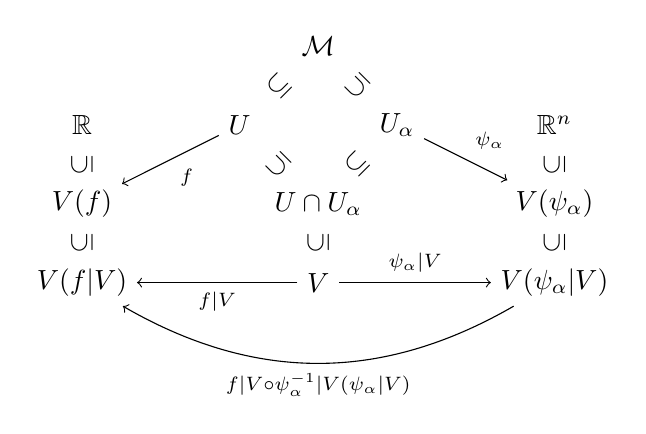
\begin{tikzpicture}[auto]
  \node (a) at ( 0, 3) {$\mathcal{M} $};
  \node (b) at (-1, 2) {$U $};
  \node (c) at ( 1, 2) {$U_\alpha $};
  \node (d) at ( 0, 1) {$U \cap U_\alpha $};
  \node (e) at ( 0, 0) {$V $};
  \node (f) at (-3, 2) {$\mathbb{R} $};
  \node (g) at (-3, 1) {$V(f) $};
  \node (h) at (-3, 0) {$V(f|V) $};
  \node (i) at ( 3, 2) {$\mathbb{R}^n $};
  \node (j) at ( 3, 1) {$V(\psi_\alpha ) $};
  \node (k) at ( 3, 0) {$V(\psi_\alpha |V ) $};
  \node (x) at (-0.5, 2.5) {\rotatebox{45}{$\subseteq $}};
  \node (x) at ( 0.5, 2.5) {\rotatebox{135}{$\subseteq $}};
  \node (x) at (-3.0, 1.5) {\rotatebox{90}{$\subseteq $}};
  \node (x) at (-0.5, 1.5) {\rotatebox{135}{$\subseteq $}};
  \node (x) at ( 0.5, 1.5) {\rotatebox{45}{$\subseteq $}};
  \node (x) at ( 3.0, 1.5) {\rotatebox{90}{$\subseteq $}};
  \node (x) at (-3.0, 0.5) {\rotatebox{90}{$\subseteq $}};
  \node (x) at ( 0.0, 0.5) {\rotatebox{90}{$\subseteq $}};
  \node (x) at ( 3.0, 0.5) {\rotatebox{90}{$\subseteq $}};
  \draw [->] (b) to node {$\scriptstyle f$} (g);
  \draw [->] (c) to node {$\scriptstyle \psi_\alpha $} (j);
  \draw [->] (e) to node {$\scriptstyle f|V$} (h);
  \draw [->] (e) to node {$\scriptstyle \psi_\alpha |V$} (k);
  \draw [->] (k) to[bend left=30] node {$\scriptstyle f|V \circ \psi_\alpha^{-1}|V(\psi_\alpha |V) $} (h);
\end{tikzpicture}
\end{center}
\begin{thm}\label{8.3.2.1}
$n$次元$C^{r}$級多様体$\left( \mathcal{M},\mathfrak{O} \right)$、その多様体$\left( \mathcal{M},\mathfrak{O} \right)$の$C^{r}$級座標近傍系$\left\{ \left( U_{\alpha},\psi_{\alpha} \right) \right\}_{\alpha \in A}$が与えられたとき、$\forall \alpha \in A$に対し、その局所座標系$\psi_\alpha $が$\psi_\alpha =\left( \psi_\alpha^i \right)_{i\in \varLambda_n }$とおかれれば、$\forall i\in \varLambda_n $に対し、その写像$\psi_\alpha^i $はその開集合$U_\alpha $で$C^r$級である。
\end{thm}
\begin{proof}
$n$次元$C^{r}$級多様体$\left( \mathcal{M},\mathfrak{O} \right)$、その多様体$\left( \mathcal{M},\mathfrak{O} \right)$の$C^{r}$級座標近傍系$\left\{ \left( U_{\alpha},\psi_{\alpha} \right) \right\}_{\alpha \in A}$が与えられたとき、$\forall \alpha \in A$に対し、その局所座標系$\psi_\alpha $が$\psi_\alpha =\left( \psi_\alpha^i \right)_{i\in \varLambda_n }$とおかれれば、$\forall i\in \varLambda_n \forall p\in U_\alpha $に対し、定理\ref{8.3.1.3}より$\exists \beta \in A$に対し\footnote{例えば、$\beta =\alpha $が挙げられる。}、$p\in U_{\alpha} \cap U_{\beta} $で、$\exists V \in \mathfrak{O}$に対し、$p\in V \subseteq U_{\alpha} \cap U_{\beta}$となるので、関数$\psi_\alpha^i \circ \psi_{\beta}^{- 1}|V\left( \psi_{\beta}|V \right):V\left( \psi_{\beta}|V \right) \rightarrow \mathbb{R}$について、$C^{r}$級多様体の定義より座標変換$f_{\left( U_{\beta},\psi_{\beta} \right) \rightarrow \left( U_{\alpha},\psi_{\alpha} \right)}$がその定義域で$C^{r}$級関数であるから、その関数$\psi_\alpha^i \circ \psi_{\beta}^{- 1}|V\left( \psi_{\beta}|V \right)$も$C^{r}$級関数である。よって、その写像$\psi_\alpha^i $はその開集合$U_\alpha $で$C^r$級である。
\end{proof}
\begin{thm}\label{8.3.2.2}
$n$次元$C^{r}$級多様体$\left( \mathcal{M},\mathfrak{O} \right)$、その多様体$\left( \mathcal{M},\mathfrak{O} \right)$の$C^{r}$級座標近傍系$\left\{ \left( U_{\alpha},\psi_{\alpha} \right) \right\}_{\alpha \in A}$が与えられたとき、$\forall \alpha \in A$に対し、$C^s $級関数$f:V\left( \psi_\alpha \right) \rightarrow \mathbb{R} $を用いた関数$f\circ \psi_\alpha : U_\alpha \rightarrow \mathbb{R} $はその開集合$U_\alpha $で$C^s$級である。
\end{thm}
\begin{proof}
$n$次元$C^{r}$級多様体$\left( \mathcal{M},\mathfrak{O} \right)$、その多様体$\left( \mathcal{M},\mathfrak{O} \right)$の$C^{r}$級座標近傍系$\left\{ \left( U_{\alpha},\psi_{\alpha} \right) \right\}_{\alpha \in A}$が与えられたとき、$\forall \alpha \in A$に対し、$C^s $級関数$f:V\left( \psi_\alpha \right) \rightarrow \mathbb{R} $を用いた関数$f\circ \psi_\alpha : U_\alpha \rightarrow \mathbb{R} $について、次のようになることから、
\begin{align*}
  f\circ \psi_\alpha \circ \psi^{-1}_\alpha |V\left( \psi_\alpha \right) &= f\circ \psi_\alpha \circ \psi^{-1}_\alpha =f 
\end{align*}
定義よりその関数$f\circ \psi_\alpha : U_\alpha \rightarrow \mathbb{R} $はその開集合$U_\alpha $で$C^s$級である。
\end{proof}
\subsubsection{写像の偏導関数}
\begin{dfn}
$n$次元$C^{r}$級多様体$\left( \mathcal{M},\mathfrak{O} \right)$、$U \in \mathfrak{O}$なるその多様体$\left( \mathcal{M},\mathfrak{O} \right)$から1次元Euclid空間$E$における位相空間$\left( \mathbb{R},\mathfrak{O}_{d_{E}} \right)$への連続写像$f:U \rightarrow \mathbb{R}$、その多様体$\left( \mathcal{M},\mathfrak{O} \right)$の$C^{r}$級座標近傍系$\left\{ \left( U_{\alpha},\psi_{\alpha} \right) \right\}_{\alpha \in A}$が与えられたとする。その局所座標系$\psi_\alpha $が$\psi_\alpha =\left( \psi_\alpha^i \right)_{i\in \varLambda_n }$とおかれれば、$\forall p\in \mathcal{M}\exists\alpha \in A$に対し、$p \in U_{\alpha}$が成り立ちその写像$f$が$1\leq s \leq r$としてその元$p$で$C^{s}$級であるとき、$i\in \varLambda_n $として次のように書くことにする。
\begin{align*}
\frac{\partial f}{\partial \psi_\alpha^i }(p) =\partial_i \left( f\circ \psi_\alpha^{-1} \right) \circ \psi_\alpha (p)
\end{align*}\par
特に、$\exists V \in \mathfrak{O}$に対し、$V \subseteq U \cap U_{\alpha}$も成り立つのであったことに注意すれば、その写像$f$が$1\leq s \leq r$としてその開集合$U$で$C^{s}$級であるとき、$i\in \varLambda_n $として次のように写像$\frac{\partial f}{\partial \psi_\alpha^i }$が定義される\footnote{写像$f:A\rightarrow B$が与えられたとき、$A'\subseteq A$なる空集合でない集合$A'$に制限された写像$f|A':A'\rightarrow B$も記法の煩雑さを避けるために$f:A'\rightarrow B$と書くことにします。また、同じ添字が2回現れたときにEinstein縮約記法も用いることにします。}。その写像$\frac{\partial f}{\partial \psi_\alpha^i } $をその写像$f$のその座標近傍$\left( U_{\alpha},\psi_{\alpha} \right) $における第$i$偏導関数という。
\begin{comment}
\begin{align*}
\frac{\partial f}{\partial \psi_\alpha^i } =\partial_i \left( f|V \circ \psi_\alpha^{-1} |V \left( \psi_\alpha |V \right)\right) \circ \psi_\alpha |V :V\rightarrow \mathbb{R} ;p\mapsto \partial_i \left( f\circ \psi_\alpha^{-1} \right) \circ \psi_\alpha (p)
\end{align*}
\end{comment}
\begin{align*}
\frac{\partial f}{\partial \psi_\alpha^i } =\partial_i \left( f\circ \psi_\alpha^{-1} \right) \circ \psi_\alpha :V\rightarrow \mathbb{R} ;p\mapsto \partial_i \left( f\circ \psi_\alpha^{-1} \right) \circ \psi_\alpha (p)
\end{align*}
\end{dfn}\par
このことは次のように表される。
\begin{center}
  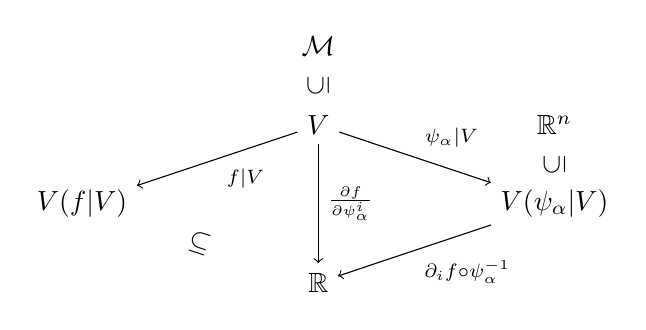
\begin{tikzpicture}[auto]
    \node (a) at ( 0, 3) {$\mathcal{M} $};
    \node (b) at ( 0, 2) {$V $};
    \node (f) at ( 0, 0) {$\mathbb{R} $};
    \node (g) at (-3, 1) {$V(f|V) $};
    \node (i) at ( 3, 2) {$\mathbb{R}^n $};
    \node (j) at ( 3, 1) {$V(\psi_\alpha |V ) $};
    \node (x) at ( 0.0, 2.5) {\rotatebox{90}{$\subseteq $}};
    \node (x) at (-1.5, 0.5) {\rotatebox{342}{$\subseteq $}};
    \node (x) at ( 3.0, 1.5) {\rotatebox{90}{$\subseteq $}};
    \draw [->] (b) to node {$\scriptstyle f|V$} (g);
    \draw [->] (b) to node {$\scriptstyle \psi_\alpha |V$} (j);
    \draw [->] (j) to node {$\scriptstyle \partial_i f\circ \psi_\alpha^{-1} $} (f);
    \draw [->] (b) to node {$\scriptstyle \frac{\partial f}{\partial \psi_\alpha^i } $} (f);
  \end{tikzpicture}
\end{center}
\begin{thm}\label{8.3.2.3}
$n$次元$C^{r}$級多様体$\left( \mathcal{M},\mathfrak{O} \right)$、$U \in \mathfrak{O}$なるその多様体$\left( \mathcal{M},\mathfrak{O} \right)$から1次元Euclid空間$E$における位相空間$\left( \mathbb{R},\mathfrak{O}_{d_{E}} \right)$への連続写像$f:U \rightarrow \mathbb{R}$、その多様体$\left( \mathcal{M},\mathfrak{O} \right)$の$C^{r}$級座標近傍系$\left\{ \left( U_{\alpha},\psi_{\alpha} \right) \right\}_{\alpha \in A}$が与えられたとする。その局所座標系$\psi_\alpha $が$\psi_\alpha =\left( \psi_\alpha^i \right)_{i\in \varLambda_n }$とおかれ、さらに、その写像$f$が、$1\leq s \leq r$としてその開集合$U$で$C^{s}$級であるとき、$\exists V\in \mathfrak{O}$に対し、$V\subseteq U\cap U_\alpha \cap U_\beta $が成り立つのであったことに注意すれば、$k\in \varLambda_n $として次式が成り立つ。
\begin{align*}
\frac{\partial f}{\partial \psi_\alpha^i } = \frac{\partial f}{\partial \psi_\beta^k } \frac{\partial \psi_\beta^k }{\partial \psi_\alpha^i } : V\rightarrow \mathbb{R}
\end{align*}
\end{thm}\par
この定理から計算方法が分かっただけではなく定義\ref{写像はCs級であることの定義}でわざわざ局所座標系を述べる必要がなかったこともわかる。
\begin{proof}
$n$次元$C^{r}$級多様体$\left( \mathcal{M},\mathfrak{O} \right)$、$U \in \mathfrak{O}$なるその多様体$\left( \mathcal{M},\mathfrak{O} \right)$から1次元Euclid空間$E$における位相空間$\left( \mathbb{R},\mathfrak{O}_{d_{E}} \right)$への連続写像$f:U \rightarrow \mathbb{R}$、その多様体$\left( \mathcal{M},\mathfrak{O} \right)$の$C^{r}$級座標近傍系$\left\{ \left( U_{\alpha},\psi_{\alpha} \right) \right\}_{\alpha \in A}$が与えられたとする。その局所座標系$\psi_\alpha $が$\psi_\alpha =\left( \psi_\alpha^i \right)_{i\in \varLambda_n }$とおかれ、さらに、その写像$f$が、$1\leq s \leq r$としてその開集合$U$で$C^{s}$級であるとき、$\exists V\in \mathfrak{O}$に対し、$V\subseteq U\cap U_\alpha \cap U_\beta $が成り立つのであったことに注意すれば、$k\in \varLambda_n $として次のようになる。
\begin{comment}
\begin{align*}
\frac{\partial f}{\partial \psi_\alpha^i } &=\partial_i \left( f|V \circ \psi_\alpha^{-1} |V \left( \psi_\alpha |V \right)\right) \circ \psi_\alpha |V \\
&=\partial_i \left( f|V \circ \left( \psi_\beta |V\right)^{-1} \circ \psi_\beta |V \circ \psi_\alpha^{-1} |V \left( \psi_\alpha |V \right)\right) \circ \psi_\alpha |V \\
&=\partial_i \left( f|V \circ \psi_\beta^{-1} |V\left( \psi_\beta |V \right) \circ \psi_\beta |V \circ \psi_\alpha^{-1} |V \left( \psi_\alpha |V \right)\right) \circ \psi_\alpha |V \\
&=\left( \partial_k \left( f|V \circ \psi_\beta^{-1} |V\left( \psi_\beta |V \right) \right) \circ \psi_\beta |V \circ \psi_\alpha^{-1} |V \left( \psi_\alpha |V \right) \right) \\
&\quad \partial_i \left( \psi_\beta^k |V \circ \psi_\alpha^{-1} |V \left( \psi_\alpha |V \right) \right) \circ \psi_\alpha |V \\
&=\left( \partial_k \left( f|V \circ \psi_\beta^{-1} |V\left( \psi_\beta |V \right) \right) \circ \psi_\beta |V \circ \left( \psi_\alpha |V \right)^{-1} \circ \psi_\alpha |V \right) \\
&\quad \left( \partial_i \left( \psi_\beta^k |V \circ \psi_\alpha^{-1} |V \left( \psi_\alpha |V \right) \right) \circ \psi_\alpha |V \right) \\
&=\left( \partial_k \left( f|V \circ \psi_\beta^{-1} |V\left( \psi_\beta |V \right) \right) \circ \psi_\beta |V \right) \\
&\quad \left( \partial_i \left( \psi_\beta^k |V \circ \psi_\alpha^{-1} |V \left( \psi_\alpha |V \right) \right) \circ \psi_\alpha |V \right) \\
&= \frac{\partial f}{\partial \psi_\beta^k } \frac{\partial \psi_\beta^k }{\partial \psi_\alpha^i }
\end{align*}
\end{comment}
\begin{align*}
  \frac{\partial f}{\partial \psi_\alpha^i } &=\partial_i \left( f\circ \psi_\alpha^{-1} \right) \circ \psi_\alpha \\
  &=\partial_i \left( f\circ \psi_\beta^{-1} \circ \psi_\beta \circ \psi_\alpha^{-1} \right) \circ \psi_\alpha \\
  &=\left( \partial_k \left( f\circ \psi_\beta^{-1} \right) \circ \psi_\beta \circ \psi_\alpha^{-1} \partial_i \left( \psi_\beta^k \circ \psi_\alpha^{-1} \right) \right) \circ \psi_\alpha \\
  &=\left( \partial_k \left( f\circ \psi_\beta^{-1} \right) \circ \psi_\beta \circ \psi_\alpha^{-1} \circ \psi_\alpha \right) \left( \partial_i \left( \psi_\beta^k \circ \psi_\alpha^{-1} \right) \circ \psi_\alpha \right) \\
  &=\left( \partial_k \left( f\circ \psi_\beta^{-1} \right) \circ \psi_\beta \right) \left( \partial_i \left( \psi_\beta^k \circ \psi_\alpha^{-1} \right) \circ \psi_\alpha \right) \\
  &= \frac{\partial f}{\partial \psi_\beta^k } \frac{\partial \psi_\beta^k }{\partial \psi_\alpha^i }
\end{align*}
\end{proof}
\begin{thm}\label{8.3.2.4}
$n$次元$C^{r}$級多様体$\left( \mathcal{M},\mathfrak{O} \right)$、その多様体$\left( \mathcal{M},\mathfrak{O} \right)$の$C^{r}$級座標近傍系$\left\{ \left( U_{\alpha},\psi_{\alpha} \right) \right\}_{\alpha \in A}$が与えられたとする。その局所座標系$\psi_\alpha $が$\psi_\alpha =\left( \psi_\alpha^i \right)_{i\in \varLambda_n }$とおかれるとき、$\exists V\in \mathfrak{O}$に対し、$V\subseteq U_\alpha \cap U_\beta $が成り立つのであったことに注意すれば、$k\in \varLambda_n $として次式が成り立つ。
\begin{align*}
  \delta_{ij} = \frac{\partial \psi_\alpha^j }{\partial \psi_\beta^k } \frac{\partial \psi_\beta^k }{\partial \psi_\alpha^i } : V\rightarrow \mathbb{R}
\end{align*}\par
さらに、次のように行列$A_{\left(U_\alpha ,\psi_\alpha \right)\rightarrow \left(U_\beta ,\psi_\beta \right)}$がおかれれば、
\begin{align*}
  A_{\left(U_\alpha ,\psi_\alpha \right)\rightarrow \left(U_\beta ,\psi_\beta \right)} = \begin{pmatrix}
    \frac{\partial \psi_\alpha^1 }{\partial \psi_\beta^1 } & \frac{\partial \psi_\alpha^2 }{\partial \psi_\beta^1 } & \cdots & \frac{\partial \psi_\alpha^n }{\partial \psi_\beta^1 } \\
    \frac{\partial \psi_\alpha^1 }{\partial \psi_\beta^2 } & \frac{\partial \psi_\alpha^2 }{\partial \psi_\beta^2 } & \cdots & \frac{\partial \psi_\alpha^n }{\partial \psi_\beta^2 } \\
    \vdots & \vdots & \ddots & \vdots \\
    \frac{\partial \psi_\alpha^1 }{\partial \psi_\beta^n } & \frac{\partial \psi_\alpha^2 }{\partial \psi_\beta^n } & \cdots & \frac{\partial \psi_\alpha^n }{\partial \psi_\beta^n } 
  \end{pmatrix} : U_\alpha \cap U_\beta \rightarrow \mathbb{R}
\end{align*}
$\det A_{\left(U_\alpha ,\psi_\alpha \right)\rightarrow \left(U_\beta ,\psi_\beta \right)} \ne 0$で$A_{\left(U_\alpha ,\psi_\alpha \right)\rightarrow \left(U_\beta ,\psi_\beta \right)}^{-1} = A_{\left(U_\beta ,\psi_\beta \right)\rightarrow \left(U_\alpha ,\psi_\alpha \right)} $が成り立つ。
\end{thm}
\begin{proof}
$n$次元$C^{r}$級多様体$\left( \mathcal{M},\mathfrak{O} \right)$、その多様体$\left( \mathcal{M},\mathfrak{O} \right)$の$C^{r}$級座標近傍系$\left\{ \left( U_{\alpha},\psi_{\alpha} \right) \right\}_{\alpha \in A}$が与えられたとする。その局所座標系$\psi_\alpha $が$\psi_\alpha =\left( \psi_\alpha^i \right)_{i\in \varLambda_n }$とおかれるとき、$\exists V\in \mathfrak{O}$に対し、$V\subseteq U_\alpha \cap U_\beta $が成り立つのであったことに注意すれば、$k\in \varLambda_n $として定理\ref{8.3.2.1}、定理\ref{8.3.2.3}より次のようになる。
\begin{align*}
  \frac{\partial \psi_\alpha^j }{\partial \psi_\alpha^i } = \frac{\partial \psi_\alpha^j }{\partial \psi_\beta^k } \frac{\partial \psi_\beta^k }{\partial \psi_\alpha^i } : V\rightarrow \mathbb{R}
\end{align*}
ここで、次のようになることから、
\begin{align*}
  \frac{\partial \psi_\alpha^j }{\partial \psi_\alpha^i } &= \partial_i \left( \psi_\alpha^j \circ \psi_\alpha^{-1} \right) \circ \psi_\alpha \\
  &= \partial_i \mathrm{pr}_j \circ \psi_\alpha = \delta_{ij} 
\end{align*}
次式が成り立つ。
\begin{align*}
  \delta_{ij} = \frac{\partial \psi_\alpha^j }{\partial \psi_\beta^k } \frac{\partial \psi_\beta^k }{\partial \psi_\alpha^i } : V\rightarrow \mathbb{R}
\end{align*}\par
さらに、次のように行列$A_{\left(U_\alpha ,\psi_\alpha \right)\rightarrow \left(U_\beta ,\psi_\beta \right)}$がおかれよう。
\begin{align*}
  A_{\left(U_\alpha ,\psi_\alpha \right)\rightarrow \left(U_\beta ,\psi_\beta \right)} = \begin{pmatrix}
    \frac{\partial \psi_\alpha^1 }{\partial \psi_\beta^1 } & \frac{\partial \psi_\alpha^2 }{\partial \psi_\beta^1 } & \cdots & \frac{\partial \psi_\alpha^n }{\partial \psi_\beta^1 } \\
    \frac{\partial \psi_\alpha^1 }{\partial \psi_\beta^2 } & \frac{\partial \psi_\alpha^2 }{\partial \psi_\beta^2 } & \cdots & \frac{\partial \psi_\alpha^n }{\partial \psi_\beta^2 } \\
    \vdots & \vdots & \ddots & \vdots \\
    \frac{\partial \psi_\alpha^1 }{\partial \psi_\beta^n } & \frac{\partial \psi_\alpha^2 }{\partial \psi_\beta^n } & \cdots & \frac{\partial \psi_\alpha^n }{\partial \psi_\beta^n } 
  \end{pmatrix} : U_\alpha \cap U_\beta \rightarrow \mathbb{R}
\end{align*}
このとき、上記の議論により次のようになる、
\begin{align*}
  \delta_{ij} = \frac{\partial \psi_\alpha^j }{\partial \psi_\beta^k } \frac{\partial \psi_\beta^k }{\partial \psi_\alpha^i } : V\rightarrow \mathbb{R},\ \ \delta_{ij} = \frac{\partial \psi_\beta^j }{\partial \psi_\alpha^k } \frac{\partial \psi_\alpha^k }{\partial \psi_\beta^i } : V\rightarrow \mathbb{R}
\end{align*}
即ち、次式が成り立つ。
\begin{align*}
  A_{\left(U_\alpha ,\psi_\alpha \right)\rightarrow \left(U_\beta ,\psi_\beta \right)} A_{\left(U_\beta ,\psi_\beta \right)\rightarrow \left(U_\alpha ,\psi_\alpha \right)} =A_{\left(U_\beta ,\psi_\beta \right)\rightarrow \left(U_\alpha ,\psi_\alpha \right)} A_{\left(U_\alpha ,\psi_\alpha \right)\rightarrow \left(U_\beta ,\psi_\beta \right)} =I_n 
\end{align*}\par
よって、$\det A_{\left(U_\alpha ,\psi_\alpha \right)\rightarrow \left(U_\beta ,\psi_\beta \right)} \ne 0$で$A_{\left(U_\alpha ,\psi_\alpha \right)\rightarrow \left(U_\beta ,\psi_\beta \right)}^{-1} = A_{\left(U_\beta ,\psi_\beta \right)\rightarrow \left(U_\alpha ,\psi_\alpha \right)} $が成り立つ。
\begin{comment}
$\det A_{\left(U_\alpha ,\psi_\alpha \right)\rightarrow \left(U_\beta ,\psi_\beta \right)} = 0$が成り立つと仮定すると、上記の議論より次のようになる。
\begin{align*}
  1 &= \det I_n =\det \begin{pmatrix}
    1 & 0 & \cdots & 0 \\
    0 & 1 & \cdots & 0 \\
    \vdots & \vdots & \ddots & \vdots \\
    0 & 0 & \cdots & 1 \\
  \end{pmatrix}\\
  &= \left| \begin{matrix}
    \frac{\partial \psi_\alpha^1 }{\partial \psi_\beta^k } \frac{\partial \psi_\beta^k }{\partial \psi_\alpha^1 } & \frac{\partial \psi_\alpha^2 }{\partial \psi_\beta^k } \frac{\partial \psi_\beta^k }{\partial \psi_\alpha^1 } & \cdots & \frac{\partial \psi_\alpha^n }{\partial \psi_\beta^k } \frac{\partial \psi_\beta^k }{\partial \psi_\alpha^1 }\\
    \frac{\partial \psi_\alpha^1 }{\partial \psi_\beta^k } \frac{\partial \psi_\beta^k }{\partial \psi_\alpha^2 } & \frac{\partial \psi_\alpha^2 }{\partial \psi_\beta^k } \frac{\partial \psi_\beta^k }{\partial \psi_\alpha^2 } & \cdots & \frac{\partial \psi_\alpha^n }{\partial \psi_\beta^k } \frac{\partial \psi_\beta^k }{\partial \psi_\alpha^2 }\\
    \vdots & \vdots & \ddots & \vdots \\
    \frac{\partial \psi_\alpha^1 }{\partial \psi_\beta^k } \frac{\partial \psi_\beta^k }{\partial \psi_\alpha^n } & \frac{\partial \psi_\alpha^2 }{\partial \psi_\beta^k } \frac{\partial \psi_\beta^k }{\partial \psi_\alpha^n } & \cdots & \frac{\partial \psi_\alpha^n }{\partial \psi_\beta^k } \frac{\partial \psi_\beta^k }{\partial \psi_\alpha^n }
  \end{matrix} \right| \\
  &= \left| \begin{matrix}
    \frac{\partial \psi_\beta^1 }{\partial \psi_\alpha^1 }& \frac{\partial \psi_\beta^2 }{\partial \psi_\alpha^1 } & \cdots & \frac{\partial \psi_\beta^n }{\partial \psi_\alpha^1 }\\
    \frac{\partial \psi_\beta^1 }{\partial \psi_\alpha^2 } & \frac{\partial \psi_\beta^2 }{\partial \psi_\alpha^2 } & \cdots & \frac{\partial \psi_\beta^n }{\partial \psi_\alpha^2 }\\
    \vdots & \vdots & \ddots & \vdots \\
    \frac{\partial \psi_\beta^1 }{\partial \psi_\alpha^n } & \frac{\partial \psi_\beta^2 }{\partial \psi_\alpha^n }\circ \psi_\alpha^{-1} & \cdots & \frac{\partial \psi_\beta^n }{\partial \psi_\alpha^n }
  \end{matrix} \right| \left| \begin{matrix}
    \frac{\partial \psi_\alpha^1 }{\partial \psi_\beta^1 } & \frac{\partial \psi_\alpha^2 }{\partial \psi_\beta^1 } & \cdots & \frac{\partial \psi_\alpha^n }{\partial \psi_\beta^1 }\\
    \frac{\partial \psi_\alpha^1 }{\partial \psi_\beta^2 } & \frac{\partial \psi_\alpha^2 }{\partial \psi_\beta^2 } & \cdots & \frac{\partial \psi_\alpha^n }{\partial \psi_\beta^2 } \\
    \vdots & \vdots & \ddots & \vdots \\
    \frac{\partial \psi_\alpha^1 }{\partial \psi_\beta^n } & \frac{\partial \psi_\alpha^2 }{\partial \psi_\beta^n } & \cdots & \frac{\partial \psi_\alpha^n }{\partial \psi_\beta^n }
  \end{matrix} \right| \\
\end{align*}
ここで、仮定より次式が成り立つので、
\begin{align*}
  \det A_{\left(U_\alpha ,\psi_\alpha \right)\rightarrow \left(U_\beta ,\psi_\beta \right)} \circ \psi_\alpha^{-1} = \left| \begin{matrix}
    \frac{\partial \psi_\alpha^1 }{\partial \psi_\beta^1 } \circ \psi_\alpha^{-1} & \frac{\partial \psi_\alpha^2 }{\partial \psi_\beta^1 } \circ \psi_\alpha^{-1} & \cdots & \frac{\partial \psi_\alpha^n }{\partial \psi_\beta^1 } \circ \psi_\alpha^{-1} \\
    \frac{\partial \psi_\alpha^1 }{\partial \psi_\beta^2 } \circ \psi_\alpha^{-1} & \frac{\partial \psi_\alpha^2 }{\partial \psi_\beta^2 } \circ \psi_\alpha^{-1} & \cdots & \frac{\partial \psi_\alpha^n }{\partial \psi_\beta^2 } \circ \psi_\alpha^{-1} \\
    \vdots & \vdots & \ddots & \vdots \\
    \frac{\partial \psi_\alpha^1 }{\partial \psi_\beta^n } \circ \psi_\alpha^{-1} & \frac{\partial \psi_\alpha^2 }{\partial \psi_\beta^n } \circ \psi_\alpha^{-1} & \cdots & \frac{\partial \psi_\alpha^n }{\partial \psi_\beta^n } \circ \psi_\alpha^{-1}
  \end{matrix} \right| =0
\end{align*}
$1 = 0$が得られるが、これは矛盾している。よって、$\det A_{\left(U_\alpha ,\psi_\alpha \right)\rightarrow \left(U_\beta ,\psi_\beta \right)} \ne 0$が成り立つ。
\end{comment}
\end{proof}
\subsubsection{関数行列式}
\begin{dfn}
$n$次元$C^{r}$級多様体$\left( \mathcal{M},\mathfrak{O} \right)$、$U \in \mathfrak{O}$なるその多様体$\left( \mathcal{M},\mathfrak{O} \right)$から1次元Euclid空間$E$における位相空間$\left( \mathbb{R},\mathfrak{O}_{d_{E}} \right)$への$1\leq s \leq r$としてその開集合$U$で$C^{s}$級な写像の族$\left\{ f_i :U \rightarrow \mathbb{R} \right\}_{i\in \varLambda_n } $、その多様体$\left( \mathcal{M},\mathfrak{O} \right)$の$C^{r}$級座標近傍系$\left\{ \left( U_{\alpha},\psi_{\alpha} \right) \right\}_{\alpha \in A}$が与えられたとする。写像$\left( f_i \right)_{i\in \varLambda_n } :U \rightarrow \mathbb{R}^n $が$f:U \rightarrow \mathbb{R}^n $\footnote{もちろん、その写像$f$がその開集合$U$で微分可能でJacobi行列をもつのであれば、その族$\left\{ f_i \right\}_{i\in \varLambda_n } $のどの元はその開集合$U$で$C^1$級です。}、その局所座標系$\psi_\alpha $が$\psi_\alpha =\left( \psi_\alpha^i \right)_{i\in \varLambda_n }$とおかれ、$U\cap U_\alpha \ne \emptyset $のとき\footnote{定理\ref{8.3.1.3}より$\exists \alpha \in A$に対し、$U\cap U_\alpha \ne \emptyset $が成り立ちます。}、次のように写像$\frac{Df}{D\psi_\alpha }$が定義される。その写像$\frac{Df}{D\psi_\alpha }$をその写像$f$のその座標近傍$\left(U_\alpha ,\psi_\alpha \right)$におけるその開集合$U$での関数行列式という。
\begin{align*}
\frac{Df}{D\psi_\alpha } =\left| \begin{matrix}
  \frac{\partial f^1 }{\partial \psi_\alpha^1 } & \frac{\partial f^1 }{\partial \psi_\alpha^2 } & \cdots & \frac{\partial f^1 }{\partial \psi_\alpha^n } \\
  \frac{\partial f^2 }{\partial \psi_\alpha^1 } & \frac{\partial f^2 }{\partial \psi_\alpha^2 } & \cdots & \frac{\partial f^2 }{\partial \psi_\alpha^n } \\
  \vdots & \vdots & \ddots & \vdots \\
  \frac{\partial f^n }{\partial \psi_\alpha^1 } & \frac{\partial f^n }{\partial \psi_\alpha^2 } & \cdots & \frac{\partial f^n }{\partial \psi_\alpha^n }
\end{matrix} \right| :U\cap U_\alpha \rightarrow \mathbb{R}
\end{align*}
\end{dfn}
\begin{thm}\label{8.3.2.5}
$n$次元$C^{r}$級多様体$\left( \mathcal{M},\mathfrak{O} \right)$、$U \in \mathfrak{O}$なるその多様体$\left( \mathcal{M},\mathfrak{O} \right)$から1次元Euclid空間$E$における位相空間$\left( \mathbb{R},\mathfrak{O}_{d_{E}} \right)$への$1\leq s \leq r$としてその開集合$U$で$C^{s}$級な写像の族$\left\{ f_i :U \rightarrow \mathbb{R} \right\}_{i\in \varLambda_n } $、その多様体$\left( \mathcal{M},\mathfrak{O} \right)$の$C^{r}$級座標近傍系$\left\{ \left( U_{\alpha},\psi_{\alpha} \right) \right\}_{\alpha \in A}$が与えられたとする。写像$\left( f_i \right)_{i\in \varLambda_n } :U \rightarrow \mathbb{R}^n $が$f:U \rightarrow \mathbb{R}^n $、その局所座標系$\psi_\alpha $が$\psi_\alpha =\left( \psi_\alpha^i \right)_{i\in \varLambda_n }$とおかれ、$U\cap U_\alpha \cap U_\beta \ne \emptyset $のとき、次式が成り立つ。
\begin{align*}
\frac{Df}{D\psi_\beta } = \det A_{\left(U_\alpha ,\psi_\alpha \right)\rightarrow \left(U_\beta ,\psi_\beta \right)} \frac{Df}{D\psi_\alpha } : U\cap U_\alpha \cap U_\beta \rightarrow \mathbb{R}
\end{align*}
特に、$\frac{Df}{D\psi_\alpha } |U\cap U_\alpha \cap U_\beta \ne 0$が成り立つのであれば、$\frac{Df}{D\psi_\beta } |U\cap U_\alpha \cap U_\beta \ne 0$も成り立つことになる。
\end{thm}
\begin{proof}
$n$次元$C^{r}$級多様体$\left( \mathcal{M},\mathfrak{O} \right)$、$U \in \mathfrak{O}$なるその多様体$\left( \mathcal{M},\mathfrak{O} \right)$から1次元Euclid空間$E$における位相空間$\left( \mathbb{R},\mathfrak{O}_{d_{E}} \right)$への$1\leq s \leq r$としてその開集合$U$で$C^{s}$級な写像の族$\left\{ f_i :U \rightarrow \mathbb{R} \right\}_{i\in \varLambda_n } $、その多様体$\left( \mathcal{M},\mathfrak{O} \right)$の$C^{r}$級座標近傍系$\left\{ \left( U_{\alpha},\psi_{\alpha} \right) \right\}_{\alpha \in A}$が与えられたとする。写像$\left( f_i \right)_{i\in \varLambda_n } :U \rightarrow \mathbb{R}^n $が$f:U \rightarrow \mathbb{R}^n $、その局所座標系$\psi_\alpha $が$\psi_\alpha =\left( \psi_\alpha^i \right)_{i\in \varLambda_n }$とおかれ、$U\cap U_\alpha \cap U_\beta \ne \emptyset $のとき、$\forall i,j\in \varLambda_n $に対し、定理\ref{8.3.2.3}より次式が成り立つ。
\begin{align*}
\frac{\partial f^i }{\partial \psi_\beta^j } = \frac{\partial f^i }{\partial \psi_\alpha^k } \frac{\partial \psi_\alpha^k }{\partial \psi_\beta^j } 
\end{align*}
したがって、次式が成り立つので、
\begin{align*}
\left| \begin{matrix}
  \frac{\partial f^1 }{\partial \psi_\beta^1 } & \frac{\partial f^1 }{\partial \psi_\beta^2 } & \cdots & \frac{\partial f^1 }{\partial \psi_\beta^n } \\
  \frac{\partial f^2 }{\partial \psi_\beta^1 } & \frac{\partial f^2 }{\partial \psi_\beta^2 } & \cdots & \frac{\partial f^2 }{\partial \psi_\beta^n } \\
  \vdots & \vdots & \ddots & \vdots \\
  \frac{\partial f^n }{\partial \psi_\beta^1 } & \frac{\partial f^n }{\partial \psi_\beta^2 } & \cdots & \frac{\partial f^n }{\partial \psi_\beta^n }
\end{matrix} \right| &= \left| \begin{matrix}
  \frac{\partial f^1 }{\partial \psi_\alpha^k } \frac{\partial \psi_\alpha^k }{\partial \psi_\beta^1 } & \frac{\partial f^1 }{\partial \psi_\alpha^k } \frac{\partial \psi_\alpha^k }{\partial \psi_\beta^2 }  & \cdots & \frac{\partial f^1 }{\partial \psi_\alpha^k } \frac{\partial \psi_\alpha^k }{\partial \psi_\beta^n }  \\
  \frac{\partial f^2 }{\partial \psi_\alpha^k } \frac{\partial \psi_\alpha^k }{\partial \psi_\beta^1 }  & \frac{\partial f^2 }{\partial \psi_\alpha^k } \frac{\partial \psi_\alpha^k }{\partial \psi_\beta^2 }  & \cdots & \frac{\partial f^2 }{\partial \psi_\alpha^k } \frac{\partial \psi_\alpha^k }{\partial \psi_\beta^n }  \\
  \vdots & \vdots & \ddots & \vdots \\
  \frac{\partial f^n }{\partial \psi_\alpha^k } \frac{\partial \psi_\alpha^k }{\partial \psi_\beta^1 }  & \frac{\partial f^n }{\partial \psi_\alpha^k } \frac{\partial \psi_\alpha^k }{\partial \psi_\beta^2 }  & \cdots & \frac{\partial f^n }{\partial \psi_\alpha^k } \frac{\partial \psi_\alpha^k }{\partial \psi_\beta^n } 
\end{matrix} \right| \\
&= \left| \begin{matrix}
  \frac{\partial f^1 }{\partial \psi_\alpha^1 } & \frac{\partial f^1 }{\partial \psi_\alpha^2 }  & \cdots & \frac{\partial f^1 }{\partial \psi_\alpha^n } \\
  \frac{\partial f^2 }{\partial \psi_\alpha^1 } & \frac{\partial f^2 }{\partial \psi_\alpha^2 } & \cdots & \frac{\partial f^2 }{\partial \psi_\alpha^n } \\
  \vdots & \vdots & \ddots & \vdots \\
  \frac{\partial f^n }{\partial \psi_\alpha^1 }  & \frac{\partial f^n }{\partial \psi_\alpha^2 }  & \cdots & \frac{\partial f^n }{\partial \psi_\alpha^n } 
\end{matrix} \right| \left| \begin{matrix}
  \frac{\partial \psi_\alpha^1 }{\partial \psi_\beta^1 } & \frac{\partial \psi_\alpha^1 }{\partial \psi_\beta^2 }  & \cdots & \frac{\partial \psi_\alpha^1 }{\partial \psi_\beta^n }  \\
  \frac{\partial \psi_\alpha^2 }{\partial \psi_\beta^1 }  & \frac{\partial \psi_\alpha^2 }{\partial \psi_\beta^2 }  & \cdots & \frac{\partial \psi_\alpha^2 }{\partial \psi_\beta^n }  \\
  \vdots & \vdots & \ddots & \vdots \\
  \frac{\partial \psi_\alpha^n }{\partial \psi_\beta^1 }  & \frac{\partial \psi_\alpha^n }{\partial \psi_\beta^2 }  & \cdots & \frac{\partial \psi_\alpha^n }{\partial \psi_\beta^n } \end{matrix} \right| \\
&= \left| \begin{matrix}
  \frac{\partial \psi_\alpha^1 }{\partial \psi_\beta^1 } & \frac{\partial \psi_\alpha^2 }{\partial \psi_\beta^1 } & \cdots & \frac{\partial \psi_\alpha^n }{\partial \psi_\beta^1 } \\
  \frac{\partial \psi_\alpha^1 }{\partial \psi_\beta^2 } & \frac{\partial \psi_\alpha^2 }{\partial \psi_\beta^2 } & \cdots & \frac{\partial \psi_\alpha^n }{\partial \psi_\beta^2 } \\
  \vdots & \vdots & \ddots & \vdots \\
  \frac{\partial \psi_\alpha^1 }{\partial \psi_\beta^n } & \frac{\partial \psi_\alpha^2 }{\partial \psi_\beta^n } & \cdots & \frac{\partial \psi_\alpha^n }{\partial \psi_\beta^n } \\
\end{matrix} \right| \left| \begin{matrix}
  \frac{\partial f^1 }{\partial \psi_\alpha^1 } & \frac{\partial f^1 }{\partial \psi_\alpha^2 }  & \cdots & \frac{\partial f^1 }{\partial \psi_\alpha^n } \\
  \frac{\partial f^2 }{\partial \psi_\alpha^1 } & \frac{\partial f^2 }{\partial \psi_\alpha^2 } & \cdots & \frac{\partial f^2 }{\partial \psi_\alpha^n } \\
  \vdots & \vdots & \ddots & \vdots \\
  \frac{\partial f^n }{\partial \psi_\alpha^1 }  & \frac{\partial f^n }{\partial \psi_\alpha^2 }  & \cdots & \frac{\partial f^n }{\partial \psi_\alpha^n } 
\end{matrix} \right|
\end{align*}
次式が成り立つ。
\begin{align*}
\frac{Df}{D\psi_\beta } = \det A_{\left(U_\alpha ,\psi_\alpha \right)\rightarrow \left(U_\beta ,\psi_\beta \right)} \frac{Df}{D\psi_\alpha } 
\end{align*}\par
特に、$\frac{Df}{D\psi_\alpha } |U\cap U_\alpha \cap U_\beta \ne 0$が成り立つのであれば、定理\ref{8.3.2.4}より$\frac{Df}{D\psi_\beta } |U\cap U_\alpha \cap U_\beta \ne 0$も成り立つことになる。
\end{proof}
\begin{thm}\label{8.3.2.6}
$n$次元$C^{r}$級多様体$\left( \mathcal{M},\mathfrak{O} \right)$、その多様体$\left( \mathcal{M},\mathfrak{O} \right)$の$C^{r}$級座標近傍系$\left\{ \left( U_{\alpha},\psi_{\alpha} \right) \right\}_{\alpha \in A}$が与えられたとする。その局所座標系$\psi_\alpha $が$\psi_\alpha =\left( \psi_\alpha^i \right)_{i\in \varLambda_n }$とおかれたとき、$\frac{D\psi_\alpha }{D\psi_\alpha } = 1 $が成り立つ。
\end{thm}
\begin{proof}
$n$次元$C^{r}$級多様体$\left( \mathcal{M},\mathfrak{O} \right)$、その多様体$\left( \mathcal{M},\mathfrak{O} \right)$の$C^{r}$級座標近傍系$\left\{ \left( U_{\alpha},\psi_{\alpha} \right) \right\}_{\alpha \in A}$が与えられたとする。その局所座標系$\psi_\alpha $が$\psi_\alpha =\left( \psi_\alpha^i \right)_{i\in \varLambda_n }$とおかれたとき、定理\ref{8.3.2.1}に注意すれば、$\forall i,j\in \varLambda_n $に対し、$\frac{\partial \psi_\alpha^i }{\partial \psi_\alpha^j } $が定義できて次のようになるので、
\begin{align*}
\frac{\partial \psi_\alpha^i }{\partial \psi_\alpha^j } &= \partial_j \left( \psi_\alpha^i \circ \psi_\alpha^{-1} \right) \circ \psi_\alpha \\
&= \partial_j \mathrm{pr}_i \circ \psi_\alpha = \delta_{ij} 
\end{align*}
$\frac{D\psi_\alpha }{D\psi_\alpha } \circ \psi_\alpha^{-1} = 1 $が成り立つ。
\end{proof}
\begin{dfn}
$n$次元$C^{r}$級多様体$\left( \mathcal{M},\mathfrak{O} \right)$、$U \in \mathfrak{O}$なるその多様体$\left( \mathcal{M},\mathfrak{O} \right)$から1次元Euclid空間$E$における位相空間$\left( \mathbb{R},\mathfrak{O}_{d_{E}} \right)$への$1\leq s \leq r$としてその開集合$U$で$C^{s}$級な写像の族$\left\{ f_i :U \rightarrow \mathbb{R} \right\}_{i\in \varLambda_n } $、その多様体$\left( \mathcal{M},\mathfrak{O} \right)$の$C^{r}$級座標近傍系$\left\{ \left( U_{\alpha},\psi_{\alpha} \right) \right\}_{\alpha \in A}$が与えられたとする。写像$\left( f_i \right)_{i\in \varLambda_n } :U \rightarrow \mathbb{R}^n $が$f:U \rightarrow \mathbb{R}^n $、その局所座標系$\psi_\alpha $が$\psi_\alpha =\left( \psi_\alpha^i \right)_{i\in \varLambda_n }$とおかれ、$U\cap U_\alpha \ne \emptyset $のとき、その写像$f$のその座標近傍$\left(U_\alpha ,\psi_\alpha \right)$におけるその開集合$U$での関数行列式$\frac{Df}{D\psi_\alpha }$が$p\in U\cap U_\alpha $なる元$p$で$\frac{Df}{D\psi_\alpha } (p) \ne 0$を満たすとき、その写像$f$をその元$p$のまわりの$C^s $級局所座標系という。
\end{dfn}
\begin{thm}\label{8.3.2.7}
$n$次元$C^{r}$級多様体$\left( \mathcal{M},\mathfrak{O} \right)$、$U \in \mathfrak{O}$なるその多様体$\left( \mathcal{M},\mathfrak{O} \right)$から1次元Euclid空間$E$における位相空間$\left( \mathbb{R},\mathfrak{O}_{d_{E}} \right)$への$1\leq s \leq r$としてその開集合$U$で$C^{s}$級な写像の族$\left\{ f_i :U \rightarrow \mathbb{R} \right\}_{i\in \varLambda_n } $、その多様体$\left( \mathcal{M},\mathfrak{O} \right)$の$C^{r}$級座標近傍系$\left\{ \left( U_{\alpha},\psi_{\alpha} \right) \right\}_{\alpha \in A}$が与えられたとする。写像$\left( f_i \right)_{i\in \varLambda_n } :U \rightarrow \mathbb{R}^n $が$f:U \rightarrow \mathbb{R}^n $、その局所座標系$\psi_\alpha $が$\psi_\alpha =\left( \psi_\alpha^i \right)_{i\in \varLambda_n }$とおかれ、$U\cap U_\alpha \ne \emptyset $のとき、その写像$f$のその座標近傍$\left(U_\alpha ,\psi_\alpha \right)$におけるその開集合$U$での関数行列式$\frac{Df}{D\psi_\alpha }$が$p\in U\cap U_\alpha $なる元$p$で$\frac{Df}{D\psi_\alpha } (p) \ne 0$を満たすとき、その部分位相空間$\left( U\cap U_\alpha ,\mathfrak{O}_{U\cap U_\alpha } \right)$におけるその元$p$のある近傍$V$が存在して、$\frac{Df}{D\psi_\alpha } |V \ne 0$が成り立つ。
\end{thm}\par
このことから、その写像$f$がその元$p$のまわりの$C^s $級局所座標系であれば、その元$p$の近傍$V$をうまくとったときのその近傍$V$の各点のまわりの$C^s $級局所座標系となる。
\begin{proof}
$n$次元$C^{r}$級多様体$\left( \mathcal{M},\mathfrak{O} \right)$、$U \in \mathfrak{O}$なるその多様体$\left( \mathcal{M},\mathfrak{O} \right)$から1次元Euclid空間$E$における位相空間$\left( \mathbb{R},\mathfrak{O}_{d_{E}} \right)$への$1\leq s \leq r$としてその開集合$U$で$C^{s}$級な写像の族$\left\{ f_i :U \rightarrow \mathbb{R} \right\}_{i\in \varLambda_n } $、その多様体$\left( \mathcal{M},\mathfrak{O} \right)$の$C^{r}$級座標近傍系$\left\{ \left( U_{\alpha},\psi_{\alpha} \right) \right\}_{\alpha \in A}$が与えられたとする。写像$\left( f_i \right)_{i\in \varLambda_n } :U \rightarrow \mathbb{R}^n $が$f:U \rightarrow \mathbb{R}^n $、その局所座標系$\psi_\alpha $が$\psi_\alpha =\left( \psi_\alpha^i \right)_{i\in \varLambda_n }$とおかれ、$U\cap U_\alpha \ne \emptyset $のとき、その写像$f$のその座標近傍$\left(U_\alpha ,\psi_\alpha \right)$におけるその開集合$U$での関数行列式$\frac{Df}{D\psi_\alpha }$が$p\in U\cap U_\alpha $なる元$p$で$\frac{Df}{D\psi_\alpha } (p) \ne 0$を満たすとき、次式が成り立つことから、
\begin{align*}
\frac{Df}{D\psi_\alpha } = \sum_{\sigma \in \mathfrak{S}_n } \mathrm{sgn} \sigma \prod_{i\in \varLambda_n } \frac{\partial f^i }{\partial \psi_\alpha^{\sigma (i)} } : U\cap U_\alpha \rightarrow \mathbb{R}
\end{align*}その関数行列式$\frac{Df}{D\psi_\alpha }$はその開集合$U\cap U_\alpha $で連続である。したがって、定理\ref{8.1.3.1}よりその元$\frac{Df}{D\psi_\alpha }(p)$の1次元Euclid空間における位相空間$\left( \mathbb{R} ,\mathfrak{O}_{d_E } \right)$におけるどの近傍$W$をとってもその値域$V\left({\frac{Df}{D\psi_\alpha } }^{-1} | W\right) $はその元$p$の近傍となる。ここで、1次元Euclid空間は距離空間なので、定理\ref{8.2.1.6}より$\exists \delta \in \mathbb{R}^+ $に対し、$B\left(\frac{Df}{D\psi_\alpha }(p) ,\delta \right) \subseteq W$が成り立つので、その値域$V\left({\frac{Df}{D\psi_\alpha } }^{-1} | B\left(\frac{Df}{D\psi_\alpha }(p) ,\delta \right) \right) $もその元$p$の近傍となる。ここで、次のように正の実数$\varepsilon$が定義されれば、
\begin{align*}
\varepsilon = \min \left\{ \frac{1}{2} \left| \frac{Df}{D\psi_\alpha }(p) \right| ,\delta \right\}
\end{align*}
$B\left(\frac{Df}{D\psi_\alpha }(p) ,\varepsilon \right) \subseteq B\left(\frac{Df}{D\psi_\alpha }(p) ,\delta \right) $が成り立つので、その値域$V\left({\frac{Df}{D\psi_\alpha } }^{-1} | B\left(\frac{Df}{D\psi_\alpha }(p) ,\varepsilon \right) \right) $もその元$p$の近傍となる。ここで、この近傍を$V$とおくと、$\forall q\in V$に対し、$\frac{Df}{D\psi_\alpha }(q) \in B\left(\frac{Df}{D\psi_\alpha }(p) ,\varepsilon \right) $が成り立つので、次のようになる。
\begin{align*}
q\in V &\Leftrightarrow \frac{Df}{D\psi_\alpha }(q) \in B\left(\frac{Df}{D\psi_\alpha }(p) ,\varepsilon \right) \\
&\Leftrightarrow \left| \frac{Df}{D\psi_\alpha }(p) - \frac{Df}{D\psi_\alpha }(q) \right| < \varepsilon\leq \frac{1}{2} \left| \frac{Df}{D\psi_\alpha }(p) \right| \\
&\Rightarrow -\frac{1}{2} \left| \frac{Df}{D\psi_\alpha }(p) \right| < \left| \frac{Df}{D\psi_\alpha }(q) \right| - \left| \frac{Df}{D\psi_\alpha }(p) \right| < \frac{1}{2} \left| \frac{Df}{D\psi_\alpha }(p) \right| \\
&\Rightarrow 0 < \frac{1}{2} \left| \frac{Df}{D\psi_\alpha }(p) \right| < \left| \frac{Df}{D\psi_\alpha }(q) \right|
\end{align*}
よって、その部分位相空間$\left( U\cap U_\alpha ,\mathfrak{O}_{U\cap U_\alpha } \right)$におけるその元$p$のある近傍$V$が存在して、$\frac{Df}{D\psi_\alpha } |V \ne 0$が成り立つ。
\end{proof}
\begin{thm}\label{8.3.2.8}
$n$次元$C^{r}$級多様体$\left( \mathcal{M},\mathfrak{O} \right)$、$U \in \mathfrak{O}$なるその多様体$\left( \mathcal{M},\mathfrak{O} \right)$から1次元Euclid空間$E$における位相空間$\left( \mathbb{R},\mathfrak{O}_{d_{E}} \right)$への$1\leq s \leq r$としてその開集合$U$で$C^{s}$級な写像の族$\left\{ f_i :U \rightarrow \mathbb{R} \right\}_{i\in \varLambda_n } $、その多様体$\left( \mathcal{M},\mathfrak{O} \right)$の$C^{r}$級座標近傍系$\left\{ \left( U_{\alpha},\psi_{\alpha} \right) \right\}_{\alpha \in A}$が与えられたとする。写像$\left( f_i \right)_{i\in \varLambda_n } :U \rightarrow \mathbb{R}^n $が$f:U \rightarrow \mathbb{R}^n $、その局所座標系$\psi_\alpha $が$\psi_\alpha =\left( \psi_\alpha^i \right)_{i\in \varLambda_n }$とおかれ、$U\cap U_\alpha \ne \emptyset $でその写像$f$のその座標近傍$\left(U_\alpha ,\psi_\alpha \right)$におけるその開集合$U$での関数行列式$\frac{Df}{D\psi_\alpha }$が$p\in U\cap U_\alpha $なる元$p$で$\frac{Df}{D\psi_\alpha } (p) \ne 0$を満たすとき、即ち、その元$p$がその写像$f$の$C^s$級局所座標系であるとき、その位相空間$\left( U\cap U_\alpha ,\mathfrak{O}_{U\cap U_\alpha } \right)$におけるその元$p$のある近傍$U'$が存在して、その組$\left(U',f\right)$がその多様体$\left(\mathcal{M},\mathfrak{O}\right)$の座標近傍となる。
\end{thm}
\begin{proof}
$n$次元$C^{r}$級多様体$\left( \mathcal{M},\mathfrak{O} \right)$、$U \in \mathfrak{O}$なるその多様体$\left( \mathcal{M},\mathfrak{O} \right)$から1次元Euclid空間$E$における位相空間$\left( \mathbb{R},\mathfrak{O}_{d_{E}} \right)$への$1\leq s \leq r$としてその開集合$U$で$C^{s}$級な写像の族$\left\{ f_i :U \rightarrow \mathbb{R} \right\}_{i\in \varLambda_n } $、その多様体$\left( \mathcal{M},\mathfrak{O} \right)$の$C^{r}$級座標近傍系$\left\{ \left( U_{\alpha},\psi_{\alpha} \right) \right\}_{\alpha \in A}$が与えられたとする。写像$\left( f_i \right)_{i\in \varLambda_n } :U \rightarrow \mathbb{R}^n $が$f:U \rightarrow \mathbb{R}^n $、その局所座標系$\psi_\alpha $が$\psi_\alpha =\left( \psi_\alpha^i \right)_{i\in \varLambda_n }$とおかれ、$U\cap U_\alpha \ne \emptyset $でその写像$f$のその座標近傍$\left(U_\alpha ,\psi_\alpha \right)$におけるその開集合$U$での関数行列式$\frac{Df}{D\psi_\alpha }$が$p\in U\cap U_\alpha $なる元$p$で$\frac{Df}{D\psi_\alpha } (p) \ne 0$を満たすとき、即ち、その元$p$がその写像$f$の$C^s$級局所座標系であるとき、$\forall i,j\in \varLambda_n $に対し、次式が成り立つので、
\begin{align*}
\frac{\partial f^i }{\partial \psi_\alpha^j } = \partial_j \left( f^i \circ \psi_\alpha^{-1} \right) \circ \psi_\alpha
\end{align*}
次式が成り立つ。
\begin{align*}
\frac{Df}{D\psi_\alpha } = \det J_{f\circ \psi_\alpha^{-1} } \circ \psi_\alpha :U\cap U_\alpha \rightarrow \mathbb{R}
\end{align*}
関数行列式$\frac{Df}{D\psi_\alpha }$が$p\in U\cap U_\alpha $なる元$p$で$\frac{Df}{D\psi_\alpha } (p) \ne 0$を満たすので、$\det J_{f\circ \psi_\alpha^{-1} } \ne 0$が成り立つ、即ち、$J_{f\circ \psi_\alpha^{-1} } :U\cap U_\alpha \rightarrow M_{nn}\left(\mathbb{R}\right)$の逆行列が存在することになる。また、それらの写像たち$f_i $いずれも$C^s$級である、即ち、それらの関数たち$f_i \circ \psi_\alpha^{-1} $いずれも$C^s $級であるので、これが成り立つならそのときに限り、その関数$f\circ \psi_\alpha^{-1}$も$C^s$級である。そこで、逆関数定理より$n$次元Euclid空間$E^n $における位相空間$\left(\mathbb{R}^n ,\mathfrak{O}_{d_{E^n}}\right)$でのある開近傍たち$V$、$W$が存在して、$f\circ \psi_\alpha^{-1} |V : V\rightarrow W$の逆関数が存在するようにすることができる。さらに、その逆関数$\left(f\circ \psi_\alpha^{-1} \right)^{-1} $も$C^s$級である。特に、その関数$f\circ \psi_\alpha^{-1} $は連続でその逆関数$\left(f\circ \psi_\alpha^{-1} \right)^{-1} $も連続であるので、その関数$f\circ \psi_\alpha^{-1} $は$n$次元Euclid空間$E^n $における部分位相空間間の同相写像となっている。そこで、$U' = V\left( \psi_\alpha^{-1} |V \right)$とすれば、その写像$\psi_\alpha $が連続なのでこれは開集合で次のようになることから、
\begin{align*}
f|U' &= f \circ \psi_\alpha^{-1} \circ \psi_\alpha |V\left( \psi_\alpha^{-1} |V \right) \\
&= f \circ \psi_\alpha^{-1} |V \circ \psi_\alpha |V\left( \psi_\alpha^{-1} |V \right) 
\end{align*}
その写像$f|U'$はその部分位相空間$\left(V\left( \psi_\alpha^{-1} |V \right) , \mathfrak{O}_{V\left( \psi_\alpha^{-1} |V \right) } \right)$からその部分位相空間$\left(V,\left(\mathfrak{O}_{d_{E^n}}\right)_{V}\right)$への同相写像$\psi_\alpha |V\left( \psi_\alpha^{-1} |V \right) $とその部分位相空間$\left(V,\left(\mathfrak{O}_{d_{E^n}}\right)_{V}\right)$からその部分位相空間$\left(W,\left(\mathfrak{O}_{d_{E^n}}\right)_{W}\right)$への同相写像の合成写像となっているので、その写像$f|U'$も同相写像である。よって、その位相空間$\left( U\cap U_\alpha ,\mathfrak{O}_{U\cap U_\alpha } \right)$におけるその元$p$のある近傍$U'$が存在して、その組$\left(U',f\right)$がその多様体$\left(\mathcal{M},\mathfrak{O}\right)$の座標近傍となる。
\end{proof}
\begin{thebibliography}{50}
\bibitem{1}
  松島与三, 多様体入門, 裳華房, 1965. 第36刷 p31-35 ISBN978-4-7853-1305-0
\bibitem{2}
  新井朝雄, 相対性理論の数理, 日本評論会, 2021. 第1版第1刷 p164-166 ISBN978-4-535-78928-9
\end{thebibliography}
\end{document}

\clearpage
\documentclass[dvipdfmx]{jsarticle}
\setcounter{section}{3}
\setcounter{subsection}{2}
\usepackage{xr}
\externaldocument{8.3.1}
\externaldocument{8.3.2}
\usepackage{amsmath,amsfonts,amssymb,array,comment,mathtools,url,docmute}
\usepackage{longtable,booktabs,dcolumn,tabularx,mathtools,multirow,colortbl,xcolor}
\usepackage[dvipdfmx]{graphics}
\usepackage{bmpsize}
\usepackage{amsthm}
\usepackage{enumitem}
\setlistdepth{20}
\renewlist{itemize}{itemize}{20}
\setlist[itemize]{label=•}
\renewlist{enumerate}{enumerate}{20}
\setlist[enumerate]{label=\arabic*.}
\setcounter{MaxMatrixCols}{20}
\setcounter{tocdepth}{3}
\newcommand{\rotin}{\text{\rotatebox[origin=c]{90}{$\in $}}}
\newcommand{\amap}[6]{\text{\raisebox{-0.7cm}{\begin{tikzpicture} 
  \node (a) at (0, 1) {$\textstyle{#2}$};
  \node (b) at (#6, 1) {$\textstyle{#3}$};
  \node (c) at (0, 0) {$\textstyle{#4}$};
  \node (d) at (#6, 0) {$\textstyle{#5}$};
  \node (x) at (0, 0.5) {$\rotin $};
  \node (x) at (#6, 0.5) {$\rotin $};
  \draw[->] (a) to node[xshift=0pt, yshift=7pt] {$\textstyle{\scriptstyle{#1}}$} (b);
  \draw[|->] (c) to node[xshift=0pt, yshift=7pt] {$\textstyle{\scriptstyle{#1}}$} (d);
\end{tikzpicture}}}}
\newcommand{\twomaps}[9]{\text{\raisebox{-0.7cm}{\begin{tikzpicture} 
  \node (a) at (0, 1) {$\textstyle{#3}$};
  \node (b) at (#9, 1) {$\textstyle{#4}$};
  \node (c) at (#9+#9, 1) {$\textstyle{#5}$};
  \node (d) at (0, 0) {$\textstyle{#6}$};
  \node (e) at (#9, 0) {$\textstyle{#7}$};
  \node (f) at (#9+#9, 0) {$\textstyle{#8}$};
  \node (x) at (0, 0.5) {$\rotin $};
  \node (x) at (#9, 0.5) {$\rotin $};
  \node (x) at (#9+#9, 0.5) {$\rotin $};
  \draw[->] (a) to node[xshift=0pt, yshift=7pt] {$\textstyle{\scriptstyle{#1}}$} (b);
  \draw[|->] (d) to node[xshift=0pt, yshift=7pt] {$\textstyle{\scriptstyle{#2}}$} (e);
  \draw[->] (b) to node[xshift=0pt, yshift=7pt] {$\textstyle{\scriptstyle{#1}}$} (c);
  \draw[|->] (e) to node[xshift=0pt, yshift=7pt] {$\textstyle{\scriptstyle{#2}}$} (f);
\end{tikzpicture}}}}
\renewcommand{\thesection}{第\arabic{section}部}
\renewcommand{\thesubsection}{\arabic{section}.\arabic{subsection}}
\renewcommand{\thesubsubsection}{\arabic{section}.\arabic{subsection}.\arabic{subsubsection}}
\everymath{\displaystyle}
\allowdisplaybreaks[4]
\usepackage{vtable}
\theoremstyle{definition}
\newtheorem{thm}{定理}[subsection]
\newtheorem*{thm*}{定理}
\newtheorem{dfn}{定義}[subsection]
\newtheorem*{dfn*}{定義}
\newtheorem{axs}[dfn]{公理}
\newtheorem*{axs*}{公理}
\renewcommand{\headfont}{\bfseries}
\makeatletter
  \renewcommand{\section}{%
    \@startsection{section}{1}{\z@}%
    {\Cvs}{\Cvs}%
    {\normalfont\huge\headfont\raggedright}}
\makeatother
\makeatletter
  \renewcommand{\subsection}{%
    \@startsection{subsection}{2}{\z@}%
    {0.5\Cvs}{0.5\Cvs}%
    {\normalfont\LARGE\headfont\raggedright}}
\makeatother
\makeatletter
  \renewcommand{\subsubsection}{%
    \@startsection{subsubsection}{3}{\z@}%
    {0.4\Cvs}{0.4\Cvs}%
    {\normalfont\Large\headfont\raggedright}}
\makeatother
\makeatletter
\renewenvironment{proof}[1][\proofname]{\par
  \pushQED{\qed}%
  \normalfont \topsep6\p@\@plus6\p@\relax
  \trivlist
  \item\relax
  {
  #1\@addpunct{.}}\hspace\labelsep\ignorespaces
}{%
  \popQED\endtrivlist\@endpefalse
}
\makeatother
\renewcommand{\proofname}{\textbf{証明}}
\usepackage{tikz,graphics}
\usepackage[dvipdfmx]{hyperref}
\usepackage{pxjahyper}
\hypersetup{
 setpagesize=false,
 bookmarks=true,
 bookmarksdepth=tocdepth,
 bookmarksnumbered=true,
 colorlinks=false,
 pdftitle={},
 pdfsubject={},
 pdfauthor={},
 pdfkeywords={}}
\begin{document}
\subsection{接vector空間}
\subsubsection{$p$-同値}
\begin{dfn}
  $n$次元多様体$\left(\mathcal{M},\mathfrak{O}\right)$の台集合$\mathcal{M}$の元$p$が与えられたとき、その元$p$の近傍$V$を用いた$C^{\infty} $級写像$f:V\rightarrow \mathbb{R} $全体の集合$C^\infty_p \left( V\right)$について、その和集合$\bigsqcup_{V\in \mathbf{V}} C^\infty_p \left( V\right)$を$C^\infty_p \mathcal{M}$と書き、さらに、その多様体$\left(\mathcal{M},\mathfrak{O}\right)$上の$C^\infty $級関数全体、即ち、和集合$\bigsqcup_{U\in \mathfrak{O} } C^\infty \left(U\right)$を$C^\infty \mathcal{M}$と書く。
\end{dfn}
\begin{thm}\label{8.3.3.1}
  $n$次元多様体$\left(\mathcal{M},\mathfrak{O}\right)$の台集合$\mathcal{M}$の元$p$が与えられたとき、$\forall a,b\in \mathbb{R} \forall f,g\in C^\infty_p \mathcal{M}$に対し、$af+bg,fg\in C^\infty_p \mathcal{M} $が成り立つ。
\end{thm}
\begin{proof}
  $n$次元多様体$\left(\mathcal{M},\mathfrak{O}\right)$の台集合$\mathcal{M}$の元$p$が与えられたとき、$\forall a,b\in \mathbb{R} \forall f,g\in C^\infty_p \mathcal{M}$に対し、それらの写像たち$f$、$g$の定義域をそれぞれ$V$、$W$とすれば、$V\cap W \in \mathbf{V} \left( p\right) $より適切に座標近傍系$\left(U,\psi\right)$がとられれば、次の関数たちは$C^\infty $級関数であり
  \begin{align*}
    f\circ \psi^{-1} |V\left(\psi | U\cap V\cap W \right) &: V\left(\psi | U\cap V\cap W \right) \rightarrow \mathbb{R}, \\
    g\circ \psi^{-1} |V\left(\psi | U\cap V\cap W \right) &: V\left(\psi | U\cap V\cap W \right) \rightarrow \mathbb{R} 
  \end{align*}
  次の関数たちも$C^\infty $級関数である。
  \begin{align*}
    af\circ \psi^{-1} +bg\circ \psi^{-1} |V\left(\psi | U\cap V\cap W \right) &: V\left(\psi | U\cap V\cap W \right) \rightarrow \mathbb{R};\psi\left(p\right) \mapsto af\left(p\right) +bg\left(p\right), \\
    \left( f\circ \psi^{-1} \right) \left( g\circ \psi^{-1} \right) |V\left(\psi | U\cap V\cap W \right) &: V\left(\psi | U\cap V\cap W \right) \rightarrow \mathbb{R} ;\psi\left(p\right) \mapsto f\left(p\right) g\left(p\right) 
  \end{align*}
  ここで、次のことが成り立つことに注意すれば、
  \begin{align*}
    af\circ \psi^{-1} +bg\circ \psi^{-1} |V\left(\psi | U\cap V\cap W \right) &= \left( af+bg \right) \circ \psi^{-1} |V\left(\psi | U\cap V\cap W \right) ,\\
    \left( f\circ \psi^{-1} \right) \left( g\circ \psi^{-1} \right) |V\left(\psi | U\cap V\cap W \right) &= fg\circ \psi^{-1} |V\left(\psi | U\cap V\cap W \right) 
  \end{align*}
  よって、これらの写像たち$af+bg$、$fg$はその元$p$の近傍で定義される写像で$C^\infty $級であり$af+bg,fg\in C^\infty_p \mathcal{M} $が成り立つ。
\end{proof}
\begin{thm}\label{8.3.3.2}
  $n$次元多様体$\left(\mathcal{M},\mathfrak{O}\right)$の台集合$\mathcal{M}$の元$p$が与えられたとき、その集合$C^\infty_p \mathcal{M} $はvector空間になりえない\footnote{なお、終集合が$\mathbb{R}$かこれの部分集合となっているような2つの写像たち$f$、$g$の実数たち$a$、$b$を用いた写像$af+bg$を次のように定義するものとしています。
  \begin{align*}
    af+bg:D\left(f\right)\cap D\left(g\right)\rightarrow \mathbb{R} ;q\mapsto af\left(q\right) +bg\left(q\right)
  \end{align*}}。
\end{thm}
\begin{proof}
  $n$次元多様体$\left(\mathcal{M},\mathfrak{O}\right)$の台集合$\mathcal{M}$の元$p$が与えられたとき、その集合$C^\infty_p \mathcal{M} $がvector空間であると仮定しよう。vector空間の公理より零vector$\mathbf{0} $が存在する。このとき、$\forall f\in C^\infty_p \mathcal{M} $に対し、$f+\mathbf{0}=f$が成り立つ。そこで、その集合$C^\infty_p \mathcal{M} $の元の定義域の和集合を$\mathcal{U}$としその写像$\mathbf{0}$の定義域がその集合$\mathcal{U}$でないとすれば、その定義域を$D\left(\mathbf{0}\right)$として$D\left(\mathbf{0}\right)\subset \mathcal{U} $が成り立つ。このとき、その集合$\mathcal{U}$はその元$p$の近傍であるので、$q\in \mathcal{U} \setminus D\left(\mathbf{0}\right)$とすれば、その集合$\mathcal{U}$の定義よりその元$q$が属するような定義域$V$をもつその集合$C^\infty_p \mathcal{M} $の元$g$が存在する。このとき、$V\cap D\left(\mathbf{0}\right) \ne V$なので、$g+\mathbf{0}=g$が成り立たない。ゆえに、その写像$\mathbf{0}$の定義域はその集合$\mathcal{U}$である。\par
  次に、その関数$f$のその可換群$\left(C^\infty_p \mathcal{M},+\right) $における逆元を$-f$とおくと、$f+\left(-f\right)=\mathbf{0}$が成り立つので、その関数$f+\left(-f\right)$の定義域はその集合$\mathcal{U}$である。ゆえに、その関数$f$の定義域は$\mathcal{U}$となる。\par
  ここで、ある座標近傍$\left(U ,\psi \right)$を用いれば、その集合$V\left(\psi\right) $は$n$次元Euclid空間における位相空間での開集合であり異なる2点$\psi \left(q\right)$、$\psi\left(r\right)$がとられることができる。このとき、その写像$\psi $は同相写像なので、$q\ne r$が成り立つ。そこで、その多様体$\left(\mathcal{M},\mathfrak{O}\right)$がHaudorff空間であることから、それらの元々$p$、$q$、$r$の互いに素な近傍たち$V_p $、$V_q $、$V_r $がとられることができる。このとき、それらの関数たち$f|V_p \sqcup V_q$、$f|V_p \sqcup V_r$もその集合$C^\infty_p \mathcal{M}$の元々である。しかしながら、それらの関数たちの定義域は$\mathcal{U}$でありえない。このことは上記の議論に矛盾する。よって、その集合$C^\infty_p \mathcal{M} $はvector空間になりえない。
\end{proof}
\begin{dfn}
  $n$次元多様体$\left(\mathcal{M},\mathfrak{O}\right)$の台集合$\mathcal{M}$の元$p$が与えられたとする。その集合$C_p\infty \mathcal{M}$の元々$f$、$g$において、$\exists V\in \mathbf{V}\left(p\right)$に対し、$f|V=g|V$が成り立つとき、それらの写像たち$f$、$g$は$p$-同値であるといい、$f\sim_p g$と書く。
\end{dfn}
\begin{thm}\label{8.3.3.3}
  $n$次元多様体$\left(\mathcal{M},\mathfrak{O}\right)$の台集合$\mathcal{M}$の元$p$が与えられたとき、その関係$\sim_p $は同値関係となる。
\end{thm}
\begin{proof}
  $n$次元多様体$\left(\mathcal{M},\mathfrak{O}\right)$の台集合$\mathcal{M}$の元$p$が与えられたとき、$\forall f\in C^\infty_p \mathcal{M}$に対し、その写像$f$の定義域を$V$とすれば、もちろん$V\in \mathbf{V}\left(p\right)$で$f|V=f|V$が成り立つ。$\forall f,g\in C^\infty_p \mathcal{M}$に対し、$f\sim_p g$が成り立つなら、$\exists V\in \mathbf{V}\left(p\right)$に対し、$f|V=g|V$が成り立つので、$g\sim_p f$が成り立つ。最後に、$\forall f,g,h\in C^\infty_p \mathcal{M}$に対し、$f\sim_p g$かつ$g\sim_p f$が成り立つなら、$\exists V,W\in \mathbf{V}\left(p\right)$に対し、$f|V=g|V$かつ$g|W=h|W$が成り立つ。そこで、$V\cap W\in \mathbf{V}\left(p\right)$で$f|V\cap W=g|V\cap W$かつ$g|V\cap W=h|V\cap W$が成り立っているので、$f|V\cap W=h|V\cap W$が成り立つ。これにより、$f\sim_p h$が得られた。
\end{proof}
\begin{thm}\label{8.3.3.4}
  $n$次元多様体$\left(\mathcal{M},\mathfrak{O}\right)$の台集合$\mathcal{M}$の元$p$が与えられたとき、次のように和とscalar倍が定義されれば、
  \begin{align*}
    +&:C^\infty_p \mathcal{M} /\sim_p \times C^\infty_p \mathcal{M} /\sim_p \rightarrow C^\infty_p \mathcal{M} /\sim_p ; \left( C_{\sim_p} \left(f\right),C_{\sim_p} \left(g\right)\right) \mapsto C_{\sim_p} \left(f+g\right) \\
    \cdot &: \mathbb{R} \times C^\infty_p \mathcal{M} /\sim_p \rightarrow C^\infty_p \mathcal{M} /\sim_p ; \left( a,C_{\sim_p } \left(f\right) \right) \mapsto C_{\sim_p} \left(af\right)
  \end{align*}
  その商集合$C^\infty_p \mathcal{M} /\sim_p $は体$\mathbb{R}$上のvector空間をなす。
\end{thm}
\begin{proof}
  $n$次元多様体$\left(\mathcal{M},\mathfrak{O}\right)$の台集合$\mathcal{M}$の元$p$が与えられたとする。次のように和とscalar倍が定義されたとき、
  \begin{align*}
    +&:C^\infty_p \mathcal{M} /\sim_p \times C^\infty_p \mathcal{M} /\sim_p \rightarrow C^\infty_p \mathcal{M} /\sim_p ; \left( C_{\sim_p} \left(f\right),C_{\sim_p} \left(g\right)\right) \mapsto C_{\sim_p} \left(f+g\right) \\
    \cdot &: \mathbb{R} \times C^\infty_p \mathcal{M} /\sim_p \rightarrow C^\infty_p \mathcal{M} /\sim_p ; \left( a,C_{\sim_p } \left(f\right) \right) \mapsto C_{\sim_p} \left(af\right)
  \end{align*}
  そのscalar倍はうまく定義されているので、その和がうまく定義されていることを示そう。$\forall f,f',g,g' \in C^\infty_p \mathcal{M}$に対し、$f\sim_p f'$かつ$g\sim_p g'$が成り立つとすれば、即ち、$C_{\sim_p} \left(f\right) =C_{\sim_p } \left(f'\right)$かつ$C_{\sim_p} \left(g\right) =C_{\sim_p } \left(g'\right)$が成り立つとすれば、$\exists V,W\in \mathbf{V} \left(p\right)$に対し、$f|V=f'|V$かつ$g|W=g'|W$が成り立っているので、$V\cap W\in \mathbf{V} \left(p\right)$に注意すれば、$\left(f+g\right)|V\cap W=\left(f'+g'\right)|V\cap W$が成り立つので、$f+g\sim_p f'+g'$が成り立つ、即ち、$C_{\sim_p } \left(f+g\right) =C_{\sim_p } \left(f'+g'\right)$が成り立つ。\par
  次に、$0:\mathcal{M} \rightarrow \mathbb{R} ;q\mapsto 0$は定数関数なので、その元$p$で$C^\infty $級である。このとき、組$\left(C^\infty_p \mathcal{M}/\sim_p,+\right)$が可換群をなすことを示そう。$\forall C_{\sim_p } \left(f\right) ,C_{\sim_p } \left(g\right) ,C_{\sim_p } \left(h\right) \in C^\infty_p \mathcal{M}/\sim_p$に対し、次のようになるかつ、
  \begin{align*}
    \left(C_{\sim_p} \left(f\right) +C_{\sim_p } \left(g\right) \right) +C_{\sim_p } \left(h\right) &=C_{\sim_p } \left(f+g\right) +C_{\sim_p } \left(h\right) \\
    &=C_{\sim_p } \left(\left(f+g\right)+h\right) \\
    &=C_{\sim_p } \left(f+\left(g+h\right)\right) \\
    &=C_{\sim_p } \left(f\right) +C_{\sim_p } \left(g+h\right) \\
    &=C_{\sim_p } \left(f\right) +\left(C_{\sim_p } \left(g\right) +C_{\sim_p } \left(h\right) \right) 
  \end{align*}
  $\forall C_{\sim_p } \left(f\right) \in C^\infty_p \mathcal{M}/\sim_p$に対し、その写像$f$の定義域を$V$とすれば、$0|V\sim_p 0$より次のようになるかつ、
  \begin{align*}
    C_{\sim_p }\left(f\right)+C_{\sim_p}\left(0\right)&=C_{\sim_p }\left(f\right)+C_{\sim_p}\left(0|V\right)\\
    &=C_{\sim_p }\left(f+0|V\right)\\
    &=C_{\sim_p }\left(f\right)
  \end{align*}
  さらに、$\forall C_{\sim_p } \left(f\right) \in C^\infty_p \mathcal{M}/\sim_p$に対し、その写像$f$の定義域を$V$とすれば、$0|V\sim_p 0$より次のようになるかつ、
  \begin{align*}
    C_{\sim_p }\left(f\right)+C_{\sim_p}\left(-f\right)&=C_{\sim_p }\left(f-f\right)\\
    &=C_{\sim_p }\left(0|V\right)\\
    &=C_{\sim_p }\left(0\right)
  \end{align*}
  $\forall C_{\sim_p } \left(f\right) ,C_{\sim_p } \left(g\right) \in C^\infty_p \mathcal{M}/\sim_p$に対し、次のようになる。
  \begin{align*}
    C_{\sim_p} \left(f\right) +C_{\sim_p } \left(g\right) &=C_{\sim_p } \left(f+g\right) \\
    &=C_{\sim_p } \left(g+f\right) \\
    &=C_{\sim_p } \left(g\right) +C_{\sim_p } \left(f\right) 
  \end{align*}
  以上の議論よりその組$\left(C^\infty_p \mathcal{M}/\sim_p,+\right)$は可換群をなす。あとは、次のことがただちに示される。
  \begin{itemize}
    \item $\forall a\in \mathbb{R} \forall C_{\sim_p }\left(f\right),C_{\sim_p }\left(g\right) \in C^\infty_p \mathcal{M}/\sim_p$に対し、$a\left(C_{\sim_p} \left(f\right)+C_{\sim_p} \left(g\right)\right)=aC_{\sim_p} \left(f\right)+aC_{\sim_p} \left(g\right)$が成り立つ。
    \item $\forall a,b\in \mathbb{R} \forall C_{\sim_p }\left(f\right)\in C^\infty_p \mathcal{M}/\sim_p$に対し、$\left(a+b\right)C_{\sim_p} \left(f\right)=aC_{\sim_p} \left(f\right)+bC_{\sim_p} \left(f\right)$が成り立つ。
    \item $\forall a,b\in \mathbb{R} \forall C_{\sim_p }\left(f\right)\in C^\infty_p \mathcal{M}/\sim_p$に対し、$\left(ab\right)C_{\sim_p} \left(f\right)=a\left(bC_{\sim_p} \left(f\right)\right)$が成り立つ。
    \item $\forall C_{\sim_p }\left(f\right)\in C^\infty_p \mathcal{M}/\sim_p$に対し、$1C_{\sim_p} \left(f\right)=C_{\sim_p} \left(f\right)$が成り立つ。
  \end{itemize}
  よって、その商集合$C^\infty_p \mathcal{M} /\sim_p $は体$\mathbb{R}$上のvector空間をなす。
\end{proof}
\begin{thm}\label{8.3.3.5}
  $n$次元多様体$\left(\mathcal{M},\mathfrak{O}\right)$の台集合$\mathcal{M}$の元$p$が与えられたとき、次のように積が定義されれば、
  \begin{align*}
    \cdot &:C^\infty_p \mathcal{M} /\sim_p \times C^\infty_p \mathcal{M} /\sim_p \rightarrow C^\infty_p \mathcal{M} /\sim_p ; \left( C_{\sim_p} \left(f\right),C_{\sim_p} \left(g\right)\right) \mapsto C_{\sim_p} \left(fg\right) 
  \end{align*}
  その商集合$C^\infty_p \mathcal{M} /\sim_p $は可換環をなす。
\end{thm}
\begin{proof}
  $n$次元多様体$\left(\mathcal{M},\mathfrak{O}\right)$の台集合$\mathcal{M}$の元$p$が与えられたとする。次のように積が定義されれば、
  \begin{align*}
    \cdot &:C^\infty_p \mathcal{M} /\sim_p \times C^\infty_p \mathcal{M} /\sim_p \rightarrow C^\infty_p \mathcal{M} /\sim_p ; \left( C_{\sim_p} \left(f\right),C_{\sim_p} \left(g\right)\right) \mapsto C_{\sim_p} \left(fg\right) 
  \end{align*}  
  その積がうまく定義されていることを示そう。$\forall f,f',g,g' \in C^\infty_p \mathcal{M}$に対し、$f\sim_p f'$かつ$g\sim_p g'$が成り立つとすれば、即ち、$C_{\sim_p} \left(f\right) =C_{\sim_p } \left(f'\right)$かつ$C_{\sim_p} \left(g\right) =C_{\sim_p } \left(g'\right)$が成り立つとすれば、$\exists V,W\in \mathbf{V} \left(p\right)$に対し、$f|V=f'|V$かつ$g|W=g'|W$が成り立っているので、$V\cap W\in \mathbf{V} \left(p\right)$に注意すれば、$\left(fg\right)|V\cap W=\left(f'g'\right)|V\cap W$が成り立つので、$fg\sim_p f'g'$が成り立つ、即ち、$C_{\sim_p } \left(fg\right) =C_{\sim_p } \left(f'g'\right)$が成り立つ。\par
  定理\ref{8.3.3.4}の証明と同様にすれば、その組$\left(C^\infty_p \mathcal{M}/\sim_p \right)$は可換群をなす。さらに、$1:\mathcal{M} \rightarrow \mathbb{R} ;q\mapsto 1$は定数関数なので、その元$p$で$C^\infty $級である。これにより、$\forall C_{\sim_p}\left(f\right),C_{\sim_p}\left(g\right),C_{\sim_p}\left(h\right)\in C^\infty_p \mathcal{M}/\sim_p$に対し、次のようになるかつ、
  \begin{align*}
    \left(C_{\sim_p}\left(f\right)C_{\sim_p}\left(g\right)\right)C_{\sim_p}\left(h\right)&=C_{\sim_p}\left(fg\right)C_{\sim_p}\left(h\right)\\
    &=C_{\sim_p}\left(\left(fg\right)h\right)\\
    &=C_{\sim_p}\left(f\left(gh\right)\right)\\
    &=C_{\sim_p}\left(f\right)C_{\sim_p}\left(gh\right)\\
    &=C_{\sim_p}\left(f\right)\left(C_{\sim_p}\left(g\right)C_{\sim_p}\left(h\right)\right)
  \end{align*}
  $\forall C_{\sim_p}\left(f\right)\in C^\infty_p \mathcal{M}/\sim_p$に対し、次のようになるかつ、
  \begin{align*}
    C_{\sim_p}\left(1\right)C_{\sim_p}\left(f\right)&=C_{\sim_p}\left(1f\right)\\
    &=C_{\sim_p}\left(f\right)
  \end{align*}
  $\forall C_{\sim_p}\left(f\right),C_{\sim_p}\left(g\right),C_{\sim_p}\left(h\right)\in C^\infty_p \mathcal{M}/\sim_p$に対し、次のようになるかつ、
  \begin{align*}
    C_{\sim_p}\left(f\right)\left(C_{\sim_p}\left(g\right)+C_{\sim_p}\left(h\right)\right)&=C_{\sim_p}\left(f\right)C_{\sim_p}\left(g+h\right)\\
    &=C_{\sim_p}\left(f\left(g+h\right)\right)\\
    &=C_{\sim_p}\left(fg+fh\right)\\
    &=C_{\sim_p}\left(fg\right)+C_{\sim_p}\left(fh\right)\\
    &=C_{\sim_p}\left(f\right)C_{\sim_p}\left(g\right)+C_{\sim_p}\left(f\right)C_{\sim_p}\left(h\right)
  \end{align*}
  $\forall C_{\sim_p}\left(f\right),C_{\sim_p}\left(g\right)\in C^\infty_p \mathcal{M}/\sim_p$に対し、次のようになる\footnote{これがあるので、積の順序を逆にしたものは示さなくても済む。}。
  \begin{align*}
    C_{\sim_p}\left(f\right)C_{\sim_p}\left(g\right)&=C_{\sim_p}\left(fg\right)\\
    &=C_{\sim_p}\left(gf\right)\\
    &=C_{\sim_p}\left(g\right)C_{\sim_p}\left(f\right)
  \end{align*}
  これにより、その商集合$C^\infty_p \mathcal{M}/\sim_p$は可換環をなす。
\end{proof}
\subsubsection{接vector空間}
\begin{axs}[接vector空間の公理]
  $n$次元多様体$\left(\mathcal{M},\mathfrak{O}\right)$の台集合$\mathcal{M}$の元$p$が与えられたとき、写像$\widetilde{v}:C^\infty_p \mathcal{M}/\sim_p \rightarrow \mathbb{R}$のうち次のことを満たすものの合成写像$\widetilde{v} \circ C_{\sim_p}$をその元$p$におけるその多様体$\left( \mathcal{M},\mathfrak{O} \right) $の接vectorといい、さらに、これ全体の集合をその元$p$におけるその多様体$\left( \mathcal{M},\mathfrak{O} \right) $の接vector空間といい$T_p \mathcal{M} $などと書く。
  \begin{itemize}
    \item その写像$\widetilde{v}$はそのvector 空間$C^\infty_p \mathcal{M}/\sim_p $からvector空間$\mathbb{R}$への線形写像である、即ち、$\forall a,b\in \mathbb{R} \forall C_{\sim_p}\left(f\right),C_{\sim_p}\left(g\right)\in C^\infty_p \mathcal{M}/\sim_p $に対し、次式が成り立つ。このことを線形性という。
    \begin{align*}
      \widetilde{v}\left( aC_{\sim_p}\left(f\right)+bC_{\sim_p}\left(g\right)\right) =a\widetilde{v}\left(C_{\sim_p}\left(f\right)\right) +b\widetilde{v}\left(C_{\sim_p}\left(g\right)\right) 
    \end{align*}
    \item $\forall C_{\sim_p} \left(f\right),C_{\sim_p} \left(g\right)\in C^\infty_p \mathcal{M}/\sim_p $に対し、次式が成り立つ。このことをLeibniz則という。
    \begin{align*}
      \widetilde{v}\left( C_{\sim_p}\left(f\right)C_{\sim_p}\left(g\right)\right) =\widetilde{v}\left(C_{\sim_p}\left(f\right)\right) g\left( p\right) +f\left( p\right) \widetilde{v}\left(C_{\sim_p}\left(g\right)\right) 
    \end{align*}
  \end{itemize}
\end{axs}
\begin{thm}\label{8.3.3.6}
  $n$次元多様体$\left(\mathcal{M},\mathfrak{O}\right)$の台集合$\mathcal{M}$の元$p$が与えられたとき、写像$v:C^\infty_p \mathcal{M}\rightarrow \mathbb{R}$がその元$p$における接vectorであるならそのときに限り、次のことを満たす。
  \begin{itemize}
    \item $\forall a,b\in \mathbb{R} \forall f,g\in C^\infty_p \mathcal{M}$に対し、次式が成り立つ。このことも線形性という。
    \begin{align*}
      v\left( af+bg\right) =av\left(f\right) +bv\left(g\right) 
    \end{align*}
    \item $\forall f,g\in C^\infty_p \mathcal{M}$に対し、次式が成り立つ。このこともLeibniz則という。
    \begin{align*}
      v\left(fg\right)=v\left(f\right)g\left( p\right)+f\left(p\right)v\left(g\right) 
    \end{align*}
    \item $\forall f,g \in C^\infty_p \mathcal{M}$に対し、$f\sim_p g$が成り立つなら、$v\left(f\right) =v\left(g\right)$が成り立つ。
  \end{itemize}
\end{thm}
\begin{proof}
  $n$次元多様体$\left(\mathcal{M},\mathfrak{O}\right)$の台集合$\mathcal{M}$の元$p$が与えられたとき、写像$v:C^\infty_p \mathcal{M}\rightarrow \mathbb{R}$がその元$p$における接vectorであるなら、公理より$v=\widetilde{v}\circ C_{\sim_p}$な写像$\widetilde{v}:C^\infty_p \mathcal{M}/\sim_p \rightarrow \mathbb{R}$が存在して、次のようになる。
  \begin{itemize}
    \item $\forall a,b\in \mathbb{R} \forall f,g\in C^\infty_p \mathcal{M}$に対し、次のようになる。
    \begin{align*}
      v\left( af+bg\right) &=\widetilde{v} \left( C_{\sim_p}\left( af+bg\right) \right) \\
      &=\widetilde{v} \left( aC_{\sim_p}\left(f\right)+bC_{\sim_p}\left(g\right) \right) \\
      &=a\widetilde{v} \left( C_{\sim_p}\left(f\right) \right) +b\widetilde{v} \left( C_{\sim_p}\left(g\right) \right) \\
      &=av\left(f\right) +bv\left(g\right) 
    \end{align*}
    \item $\forall f,g\in C^\infty_p \mathcal{M}$に対し、次のようになる。
    \begin{align*}
      v\left(fg\right)&=\widetilde{v}\left(C_{\sim_p} \left(fg\right)\right)\\
      &=\widetilde{v}\left( C_{\sim_p}\left(f\right)C_{\sim_p}\left(g\right)\right) \\
      &=\widetilde{v}\left(C_{\sim_p}\left(f\right)\right) g\left( p\right) +f\left( p\right) \widetilde{v}\left(C_{\sim_p}\left(g\right)\right) \\
      &=v\left(f\right)g\left( p\right)+f\left(p\right)v\left(g\right) 
    \end{align*}
    \item $\forall f,g \in C^\infty_p \mathcal{M}$に対し、$f\sim_p g$が成り立つなら、$C_{\sim_p }\left(f\right)=C_{\sim_p } \left(g\right)$より$v\left(f\right) =\widetilde{v}\left(C_{\sim_p }\left(f\right)\right)=\widetilde{v}\left(C_{\sim_p }\left(g\right)\right)=v\left(g\right)$が成り立つ。
  \end{itemize}\par
  一方で、その商集合$C^\infty_p \mathcal{M}/\sim_p$の元$C_{\sim_p} f$から$g\in C_{\sim_p}\left(f\right)$な写像$g$をとって実数$v\left(g\right)$へうつす写像$\widetilde{v}:C^\infty_p \mathcal{M}/\sim_p \rightarrow \mathbb{R}$が考えられよう。これはうまく定義されている。実際、$\forall C_{\sim_p} \left(f\right)\in C^\infty_p \mathcal{M}/\sim_p$に対し、その同値類$C_{\sim_p} \left(f\right)$の元々$g$、$h$がとられれば、$f\sim_p g\sim_p h$より$v\left(f\right)=v\left(g\right)=v\left(h\right)$が成り立つ。このとき、次のようになる。
  \begin{itemize}
    \item $\forall a,b\in \mathbb{R} \forall C_{\sim_p}\left(f\right),C_{\sim_p}\left(g\right)\in C^\infty_p \mathcal{M}/\sim_p $に対し、次のようになる。
    \begin{align*}
      \widetilde{v}\left( aC_{\sim_p}\left(f\right)+bC_{\sim_p}\left(g\right)\right) &=\widetilde{v}\left( C_{\sim_p}\left(af+bg\right)\right) \\
      &=v\left(af+bg\right) \\
      &=av\left(f\right)+bv\left(g\right)\\
      &=a\widetilde{v}\left(C_{\sim_p}\left(f\right)\right) +b\widetilde{v}\left(C_{\sim_p}\left(g\right)\right) 
    \end{align*}
    \item $\forall C_{\sim_p} \left(f\right),C_{\sim_p} \left(g\right)\in C^\infty_p \mathcal{M}/\sim_p $に対し、次のようになる。
    \begin{align*}
      \widetilde{v}\left( C_{\sim_p}\left(f\right)C_{\sim_p}\left(g\right)\right) &= \widetilde{v}\left( C_{\sim_p}\left(fg\right)\right) \\
      &=v\left(fg\right) \\
      &=v\left(f\right) g\left( p\right) +f\left( p\right) v\left(g\right) \\
      &=\widetilde{v}\left(C_{\sim_p}\left(f\right)\right) g\left( p\right) +f\left( p\right) \widetilde{v}\left(C_{\sim_p}\left(g\right)\right) 
    \end{align*}
  \end{itemize}
\end{proof}
\begin{thm}\label{8.3.3.7}
  $n$次元多様体$\left(\mathcal{M},\mathfrak{O}\right)$の台集合$\mathcal{M}$の元$p$が与えられたとき、その元$p$におけるその多様体$\left( \mathcal{M},\mathfrak{O} \right) $の接vector空間$T_p \mathcal{M}$において、次のように和とscalar倍が定義されれば、
  \begin{align*}
    +&:T_p \mathcal{M} \times T_p \mathcal{M} \rightarrow T_p \mathcal{M} ; \left( v,w\right) \mapsto v+w:C^\infty_p \mathcal{M} \rightarrow \mathbb{R} ; f\mapsto v\left(f\right) +w\left(f\right) \\
    \cdot &: \mathbb{R} \times T_p \mathcal{M} \rightarrow T_p \mathcal{M} ; \left( \xi,v\right) \mapsto \xi v:C^\infty_p \mathcal{M} \rightarrow \mathbb{R} ; f\mapsto \xi v\left(f\right) 
  \end{align*}
  その接vector空間$T_p \mathcal{M}$は体$\mathbb{R}$上のvector空間をなす。
\end{thm}
\begin{proof}
  $n$次元多様体$\left(\mathcal{M},\mathfrak{O}\right)$の台集合$\mathcal{M}$の元$p$が与えられたとき、その元$p$におけるその多様体$\left( \mathcal{M},\mathfrak{O} \right) $の接vector空間$T_p \mathcal{M}$において、次のように和とscalar倍が定義されれば、
  \begin{align*}
    +&:T_p \mathcal{M} \times T_p \mathcal{M} \rightarrow T_p \mathcal{M} ; \left( v,w\right) \mapsto v+w:C^\infty_p \mathcal{M} \rightarrow \mathbb{R} ; f\mapsto v\left(f\right) +w\left(f\right) \\
    \cdot &: \mathbb{R} \times T_p \mathcal{M} \rightarrow T_p \mathcal{M} ; \left( \xi,v\right) \mapsto \xi v:C^\infty_p \mathcal{M} \rightarrow \mathbb{R} ; f\mapsto \xi v\left(f\right) 
  \end{align*}
  これがうまく定義されていることを示そう。このとき、$\forall v,w\in T_p \mathcal{M}$に対し、和$v+w$が定義されれば、次のようになる。
  \begin{itemize}
    \item $\forall a,b\in \mathbb{R} \forall f,g\in C^\infty_p \mathcal{M}$に対し、次のようになる。
    \begin{align*}
      \left(v+w\right) \left(af+bg\right) &= v \left(af+bg\right) +w\left(af+bg\right) \\
      &= av\left(f\right) +bv\left(g\right) +aw\left(f\right) +bw\left(g\right) \\
      &= a\left(v+w\right) \left(f\right) +b\left(v+w\right) \left(g\right)
    \end{align*}
    \item $\forall f,g\in C^\infty_p \mathcal{M}$に対し、次のようになる。
    \begin{align*}
      \left(v+w\right) \left(fg\right) &= v \left(fg\right) +w\left(fg\right) \\
      &= v\left(f\right) g\left(p\right) +f\left(p\right) v\left(g\right) +w\left(f\right) g\left(p\right) +f\left(p\right) w\left(g\right) \\
      &= \left(v+w\right)\left(f\right) g\left(p\right) +f\left(p\right) \left(v+w\right)\left(g\right) 
    \end{align*}
    \item $\forall f,g\in C^\infty_p \mathcal{M}$に対し、$f\sim_p g$が成り立つなら、次のようになる。
    \begin{align*}
      \left(v+w\right) \left(f\right) &= v \left(f\right) +w\left(f\right) \\
      &=v\left(g\right) +w\left(g\right) \\ 
      &=\left(v+w\right)\left(g\right) 
    \end{align*}
\end{itemize}
  ゆえに、定理\ref{8.3.3.6}より$v+w\in T_p \mathcal{M}$が成り立つ。\par
  また、$\forall \xi \in \mathbb{R}\forall v\in T_p \mathcal{M}$に対し、scalar倍$\xi v$が定義されれば、次のようになる。
  \begin{itemize}
    \item $\forall a,b\in \mathbb{R} \forall f,g\in C^\infty_p \mathcal{M}$に対し、次のようになる。
    \begin{align*}
      \xi v\left(af+bg\right) &= \xi \left( av\left(f\right) +bv\left(g\right) \right) \\
      &= a\xi v\left(f\right) +b\xi v\left(g\right)
    \end{align*}
    \item $\forall f,g\in C^\infty_p \mathcal{M}$に対し、次のようになる。
    \begin{align*}
      \xi v\left(fg\right) &= \xi \left( v\left(f\right) g\left(p\right) +f\left(p\right) v\left(g\right) \right)\\
      &= \xi v\left(f\right) g\left(p\right) +f\left(p\right) \xi v\left(g\right) 
    \end{align*}
    \item $\forall f,g\in C^\infty_p \mathcal{M}$に対し、$f\sim_p g$が成り立つなら、$\xi v\left(f\right) = \xi v\left(g\right)$が成り立つ。
    \end{itemize}
  ゆえに、定理\ref{8.3.3.6}より$\xi v\in T_p \mathcal{M}$が成り立つ。\par
  あとは、次のように写像$0$が定義されれば、
  \begin{align*}
    0:C^\infty_p \mathcal{M} \rightarrow \mathbb{R};f\mapsto 0
  \end{align*}
  次のことがただちに示される。
  \begin{itemize}
    \item その集合$T_p \mathcal{M}$を用いた組$\left(T_p \mathcal{M},+\right)$は可換群をなす。
    \item $\forall \xi \in \mathbb{R} \forall v,w\in T_p \mathcal{M}$に対し、$\xi \left(v+w\right)=\xi v+\xi w$が成り立つ。
    \item $\forall \xi ,\eta \in \mathbb{R} \forall v\in T_p \mathcal{M}$に対し、$\left(\xi +\eta\right)v=\xi v+\eta v$が成り立つ。
    \item $\forall \xi ,\eta \in \mathbb{R} \forall v\in T_p \mathcal{M}$に対し、$\left(\xi \eta\right)v=\xi \left( \eta v\right) $が成り立つ。
    \item $\forall v\in T_p \mathcal{M}$に対し、$1v=v$が成り立つ。
  \end{itemize}
\end{proof}
\begin{thm}\label{8.3.3.8}
  $n$次元多様体$\left(\mathcal{M},\mathfrak{O}\right)$の台集合$\mathcal{M}$の元$p$が与えられたとき、$\forall v\in T_p \mathcal{M} \exists V\in \mathbf{V} \left(p\right) \forall f\in C^\infty_p \mathcal{M}$に対し、その写像$f|V:V\rightarrow \mathbb{R}$が定数関数となっているとき、$v\left(f\right)=0$が成り立つ。
\end{thm}
\begin{proof}
  $n$次元多様体$\left(\mathcal{M},\mathfrak{O}\right)$の台集合$\mathcal{M}$の元$p$が与えられたとき、$\forall v\in T_p \mathcal{M} \exists V\in \mathbf{V} \left(p\right) \forall f\in C^\infty_p \mathcal{M}$に対し、その写像$f|V:V\rightarrow \mathbb{R}$が定数関数となっているとき、$\forall q\in V$に対し、$C=f\left(q\right)$とおき、さらに、$\forall c\in \mathbb{R}$に対し、写像$c$を次のように定義すると、
  \begin{align*}
    c:\mathcal{M} \rightarrow \mathbb{R} ;q\mapsto c
  \end{align*}
  $f\sim_p C$となっており、したがって、次のようになる。
  \begin{align*}
    v\left(C\right) &=v\left(C\cdot 1\right) \\
    &=v\left(C\right) \cdot 1+C\cdot v\left(1\right) \\
    &=v\left(C\right) +v\left(C\right)
  \end{align*}
  これにより、$v\left(f\right)=v\left(C\right)=0$が得られる。
\end{proof}
\begin{dfn}
  $n$次元多様体$\left(\mathcal{M},\mathfrak{O}\right)$の台集合$\mathcal{M}$の元$p$が与えられたとき、$p\in U$、$\psi =\left(\psi^i \right)_{i\in \varLambda_n }$なる座標近傍$\left(U,\psi\right)$を用いて次の写像$\left. \frac{\partial}{\partial \psi^i }\right|_p $が定義される。
  \begin{align*}
    \left. \frac{\partial}{\partial \psi^i }\right|_p :C^\infty_p \mathcal{M} \rightarrow \mathbb{R} ;f\mapsto \frac{\partial f}{\partial \psi^i } \left(p\right)
  \end{align*}
  その写像$\left. \frac{\partial}{\partial \psi^i }\right|_p $をその元$p$におけるその座標近傍$\left(U,\psi\right)$での第$i$偏微分作用素という。
\end{dfn}
\begin{thm}\label{8.3.3.9}
  $n$次元多様体$\left(\mathcal{M},\mathfrak{O}\right)$の台集合$\mathcal{M}$の元$p$が与えられたとき、その元$p$における$\psi =\left(\psi^i \right)_{i\in \varLambda_n }$なる座標近傍$\left(U,\psi\right)$での第$i$偏微分作用素$\left. \frac{\partial}{\partial \psi^i }\right|_p $はその元$p$における接vectorである。
\end{thm}
\begin{proof}
  $n$次元多様体$\left(\mathcal{M},\mathfrak{O}\right)$の台集合$\mathcal{M}$の元$p$が与えられたとき、その元$p$における$\psi =\left(\psi^i \right)_{i\in \varLambda_n }$なる座標近傍$\left(U,\psi\right)$での第$i$偏微分作用素$\left. \frac{\partial}{\partial \psi^i }\right|_p $について、次のようになる。
  \begin{itemize}
    \item $\forall a,b\in \mathbb{R} \forall f,g \in C^\infty_p \mathcal{M} $に対し、次のようになる。
    \begin{align*}
      \left. \frac{\partial}{\partial \psi^i }\right|_p \left(af+bg\right) &= \frac{\partial }{\partial \psi^i } \left(af+bg\right) \left(p\right) \\
      &=a\frac{\partial f}{\partial \psi^i } \left(p\right) +b\frac{\partial g}{\partial \psi^i }\left(p\right) \\
      &=a\left. \frac{\partial }{\partial \psi^i } \right|_p \left(f\right) +b\left. \frac{\partial }{\partial \psi^i } \right|_p \left(g\right) 
    \end{align*}
    \item $\forall f,g \in C^\infty_p \mathcal{M} $に対し、次のようになる。
    \begin{align*}
      \left. \frac{\partial}{\partial \psi^i }\right|_p \left(fg\right) &= \frac{\partial }{\partial \psi^i } \left(fg\right) \left(p\right) \\
      &= \partial_i \left(fg\circ \psi^{-1} \right) \circ \psi \left(p\right) \\
      &= \partial_i \left(\left(f\circ \psi^{-1} \right) \left(g\circ \psi^{-1} \right)\right) \circ \psi \left(p\right) \\
      &= \left( \partial_i \left(f\circ \psi^{-1} \right) g\circ \psi^{-1} +f\circ \psi^{-1} \partial_i \left(g\circ \psi^{-1} \right)\right) \circ \psi \left(p\right) \\
      &= \partial_i \left(f\circ \psi^{-1} \right) \circ \psi \left(p\right) g\left(p\right) +f\left(p\right) \partial_i \left(g\circ \psi^{-1} \right) \circ \psi \left(p\right) \\
      &=\frac{\partial f}{\partial \psi^i } \left(p\right) g\left(p\right) +f\left(p\right) \frac{\partial g}{\partial \psi^i } \left(p\right) \\
      &=\left. \frac{\partial}{\partial \psi^i }\right|_p \left(f\right) g\left(p\right) +f\left(p\right) \left. \frac{\partial}{\partial \psi^i }\right|_p \left(g\right)
    \end{align*}
    \item $\forall f,g\in C^\infty_p \mathcal{M}$に対し、$f\sim_p g$が成り立つなら、$\exists V\in \mathbf{V} \left(p\right)$に対し、$f|V=g|V$が成り立つので、次のようになる。
    \begin{align*}
      \left. \frac{\partial}{\partial \psi^i } \right|_p \left(f\right) =\frac{\partial f}{\partial \psi^i } \left(p\right) =\frac{\partial f|V}{\partial \psi^i } \left(p\right) =\frac{\partial g|V}{\partial \psi^i } \left(p\right) =\frac{\partial g}{\partial \psi^i } \left(p\right) =\left. \frac{\partial}{\partial \psi^i } \right|_p \left(g\right)
    \end{align*}
  \end{itemize}
  以上、定理\ref{8.3.3.6}より$\left. \frac{\partial }{\partial \psi^i }\right|_p \in T_p \mathcal{M}$が成り立つ。
\end{proof}
\begin{thm}\label{8.3.3.10}
  $n$次元多様体$\left(\mathcal{M},\mathfrak{O}\right)$の台集合$\mathcal{M}$の元$p$が与えられたとき、その元$p$における$\psi =\left(\psi^i \right)_{i\in \varLambda_n }$なる座標近傍$\left(U,\psi\right)$での第$i$偏微分作用素$\left. \frac{\partial}{\partial \psi^i }\right|_p $からなる組$\left\langle \left. \frac{\partial}{\partial \psi^i }\right|_p \right\rangle_{i\in \varLambda_n} $はその接vector空間$T_p \mathcal{M}$の基底で$k\in \varLambda_n $として、$\forall v\in T_p \mathcal{M}$に対し、次式が成り立つ。
  \begin{align*}
    v=v\left(\psi^k \right) \left. \frac{\partial }{\partial \psi^k } \right|_p 
  \end{align*}
  特に、$\dim T_p \mathcal{M} =n$が成り立つ。
\end{thm}
\begin{dfn}
  $n$次元多様体$\left(\mathcal{M},\mathfrak{O}\right)$の台集合$\mathcal{M}$の元$p$が与えられたとき、その元$p$における$\psi =\left(\psi^i \right)_{i\in \varLambda_n }$なる座標近傍$\left(U,\psi\right)$での第$i$偏微分作用素$\left. \frac{\partial}{\partial \psi^i }\right|_p $からなる基底$\left\langle \left. \frac{\partial}{\partial \psi^i }\right|_p \right\rangle_{i\in \varLambda_n} $をその元$p$における座標近傍$\left(U,\psi\right)$での自然標構、自然基底という。
\end{dfn}
\begin{proof}
  $n$次元多様体$\left(\mathcal{M},\mathfrak{O}\right)$の台集合$\mathcal{M}$の元$p$が与えられたとき、その元$p$における$\psi =\left(\psi^i \right)_{i\in \varLambda_n }$なる座標近傍$\left(U,\psi\right)$での第$i$偏微分作用素$\left. \frac{\partial}{\partial \psi^i }\right|_p $からなる組$\left\langle \left. \frac{\partial}{\partial \psi^i }\right|_p \right\rangle_{i\in \varLambda_n} $が与えられたとき、$k\in \varLambda_n $、$c_k \in \mathbb{R}$として$c_k \left. \frac{\partial }{\partial \psi^k } \right|_p =0$が成り立つなら、$\forall i\in \varLambda_n $に対し、$\psi^i \in C^\infty_p \mathcal{M}$が成り立つので、次のようになる。
  \begin{align*}
    0 &= c_k \left. \frac{\partial }{\partial \psi^k } \right|_p \left( \psi^i \right) \\
    &= c_k \frac{\partial \psi^i }{\partial \psi^k } \left(p\right) \\
    &= c_k \partial_k \left( \psi^i \circ \psi^{-1} \right) \circ \psi \left( p \right)\\
    &= c_k \delta_{ik} = c_i 
  \end{align*}
  これにより、その組$\left\langle \left. \frac{\partial}{\partial \psi^i }\right|_p \right\rangle_{i\in \varLambda_n} $は線形独立である。\par
  一方で、その集合$V\left(\psi\right)$は開集合であるので、$\exists \varepsilon \in \mathbb{R}^+$に対し、$U\left(\psi\left(p\right),\varepsilon\right)\subseteq V\left(\psi\right)$が成り立つ\footnote{$U\left(\psi\left(p\right),\varepsilon\right)$は中心$\psi\left(p\right)$、半径$\varepsilon$の開球です。}。そこで、その関数$f\circ \psi^{-1}$は$C^2$級でもあるので、Taylorの定理より$h=\left(h^i \right)_{i\in \varLambda_n } :V\left(\psi^{-1}|U\left(\psi\left(p\right),\varepsilon\right)\right) \rightarrow \mathbb{R} ;q\mapsto \psi \left(q\right) -\psi \left(p\right)$とすれば、$\forall q\in V\left(\psi^{-1}|U\left(\psi\left(p\right),\varepsilon\right)\right)\exists c\in \left(0,1\right)$に対し、次式が成り立つ、
  \begin{align*}
    f\circ \psi^{-1} \left(\psi \left(q\right) \right) &=f\circ \psi^{-1} \left(\psi\left(p\right)\right) +\partial_k \left(f\circ \psi^{-1}\right) \left(\psi\left(p\right)\right) h^k \left(q \right) \\
    &\quad +\frac{1}{2}\partial_{kl} \left(f\circ \psi^{-1}\right) \left(\psi\left(p\right) +ch\left(q\right)\right) h^k \left(q\right) h^l \left(q\right)
  \end{align*}
  即ち、次式が成り立つ。
  \begin{align*}
    f\left(q\right) &=f\left(p\right) +\partial_k \left(f\circ \psi^{-1}\right) \circ \psi\left(p\right) h^k \left(q\right) +\frac{1}{2}\partial_{kl} \left(f\circ \psi^{-1}\right) \left(\psi\left(p\right) +ch\left(q\right)\right) h^k \left(q\right) h^l \left(q\right) \\
    &=f\left(p\right) +\frac{\partial f}{\partial \psi^k } \left(p\right) h^k \left(q\right) +\frac{1}{2}\partial_{kl} \left(f\circ \psi^{-1}\right) \left(\psi\left(p\right) +ch\left(q\right)\right) h^k \left(q\right) h^l \left(q\right) 
  \end{align*}
  これを写像とみれば、次のようになる。
  \begin{align*}
    f|V\left(\psi^{-1}|U\left(\psi\left(p\right),\varepsilon\right)\right) =f\left(p\right) +\frac{\partial f}{\partial \psi^k } \left(p\right) h^k +\frac{1}{2}\partial_{kl} \left(f\circ \psi^{-1}\right) \left(\psi\left(p\right) +ch \right) h^k h^l 
  \end{align*} 
  したがって、次のようになる。
  \begin{align*}
    v\left(f\right) &=v\left(f\left(p\right) +\frac{\partial f}{\partial \psi^k } \left(p\right) h^k +\frac{1}{2}\partial_{kl} \left(f\circ \psi^{-1}\right) \left(\psi\left(p\right) +ch \right) h^k h^l \right) \\
    &=v\left(f\left(p\right) \right)+\frac{\partial f}{\partial \psi^k } \left(p\right) v\left(h^k \right) +\frac{1}{2}v\left(\partial_{kl} \left(f\circ \psi^{-1}\right) \left(\psi\left(p\right) +ch \right) h^k h^l \right) \\
    &=v\left(f\left(p\right) \right)+\frac{\partial f}{\partial \psi^k } \left(p\right) v\left(h^k \right) \\
    &\quad +\frac{1}{2}v\left(\partial_{kl} \left(f\circ \psi^{-1}\right) \left(\psi\left(p\right) +ch \right) \right) h^k \left(p\right) h^l \left(p\right) \\
    &\quad +\frac{1}{2}\partial_{kl} \left(f\circ \psi^{-1}\right) \left(\psi\left(p\right) +ch\left(p\right) \right) v\left(h^k\right) h^l \left(p\right) \\
    &\quad +\frac{1}{2}\partial_{kl} \left(f\circ \psi^{-1}\right) \left(\psi\left(p\right) +ch\left(p\right) \right) h^k \left(p\right) v\left(h^l\right) \\
    &=v\left(f\left(p\right) \right)+\frac{\partial f}{\partial \psi^k } \left(p\right) v\left(\psi^k -\psi^k  \left(p\right) \right) \\
    &\quad +\frac{1}{2}v\left(\partial_{kl} \left(f\circ \psi^{-1}\right) \left(\psi\left(p\right) +ch \right) \right) \left(\psi^k \left(p\right) -\psi^k  \left(p\right)\right) \left(\psi^l \left(p\right) -\psi^l \left(p\right)\right)\\
    &\quad +\frac{1}{2}\partial_{kl} \left(f\circ \psi^{-1}\right) \left(\psi\left(p\right) +ch\left(p\right) \right) v\left(\psi^k-\psi^k  \left(p\right)\right) \left(\psi^l \left(p\right) -\psi^l \left(p\right)\right)\\
    &\quad +\frac{1}{2}\partial_{kl} \left(f\circ \psi^{-1}\right) \left(\psi\left(p\right) +ch\left(p\right) \right) \left(\psi^k \left(p\right) -\psi^k  \left(p\right)\right) v\left(\psi^l -\psi^l \left(p\right)\right) \\
    &=v\left(f\left(p\right) \right)+\frac{\partial f}{\partial \psi^k } \left(p\right) \left(v\left(\psi^k \right)-v\left(\psi^k \left(p\right) \right)\right) \\
    &\quad +\frac{1}{2}v\left(\partial_{kl} \left(f\circ \psi^{-1}\right) \left(\psi\left(p\right) +ch \right) \right) \left(\psi^k \left(p\right) -\psi^k  \left(p\right)\right) \left(\psi^l \left(p\right) -\psi^l \left(p\right)\right)\\
    &\quad +\frac{1}{2}\partial_{kl} \left(f\circ \psi^{-1}\right) \left(\psi\left(p\right) +ch\left(p\right) \right) \left(v\left(\psi^k \right)-v\left(\psi^k \left(p\right) \right)\right)  \left(\psi^l \left(p\right) -\psi^l \left(p\right)\right)\\
    &\quad +\frac{1}{2}\partial_{kl} \left(f\circ \psi^{-1}\right) \left(\psi\left(p\right) +ch\left(p\right) \right) \left(\psi^k \left(p\right) -\psi^k  \left(p\right)\right) \left(v\left(\psi^l \right)-v\left(\psi^l \left(p\right) \right)\right) \\
    &=0+\frac{\partial f}{\partial \psi^k } \left(p\right) \left(v\left(\psi^k \right)-0\right) \\
    &\quad +\frac{1}{2}v\left(\partial_{kl} \left(f\circ \psi^{-1}\right) \left(\psi\left(p\right) +ch \right) \right) \cdot 0\cdot 0\\
    &\quad +\frac{1}{2}\partial_{kl} \left(f\circ \psi^{-1}\right) \left(\psi\left(p\right) +ch\left(p\right) \right) \left(v\left(\psi^k \right)-v\left(\psi^k \left(p\right) \right)\right) \cdot 0\\
    &\quad +\frac{1}{2}\partial_{kl} \left(f\circ \psi^{-1}\right) \left(\psi\left(p\right) +ch\left(p\right) \right) \cdot 0 \cdot \left(v\left(\psi^l \right)-v\left(\psi^l \left(p\right) \right)\right) \\
    &=v\left(\psi^k \right) \frac{\partial f}{\partial \psi^k } \left(p\right) =v\left(\psi^k \right) \left. \frac{\partial}{\partial \psi^k } \right|_p \left(f\right)
  \end{align*}
  これにより、次式が成り立つので、
  \begin{align*}
    v=v\left(\psi^k \right) \left. \frac{\partial }{\partial \psi^k } \right|_p 
  \end{align*}
  その接vector空間$T_p \mathcal{M}$はそれらの接vectorたち$\left. \frac{\partial }{\partial \psi^i } \right|_p $によって張られている。\par
  よって、その組$\left\langle \left. \frac{\partial}{\partial \psi^i }\right|_p \right\rangle_{i\in \varLambda_n} $はその接vector空間$T_p \mathcal{M}$の基底で$k\in \varLambda_n $として、$\forall v\in T_p \mathcal{M}$に対し、次式が成り立つ。
  \begin{align*}
    v=v\left(\psi^k \right) \left. \frac{\partial }{\partial \psi^k } \right|_p 
  \end{align*}
  特に、$\dim T_p \mathcal{M} =n$が成り立つ。
\end{proof}
\begin{thm}\label{8.3.3.11}
  $n$次元多様体$\left(\mathcal{M},\mathfrak{O}\right)$の台集合$\mathcal{M}$の元$p$が与えられたとき、その元$p$における座標近傍$\left(U_\alpha,\psi_\alpha \right)$での自然標構$\left\langle \left. \frac{\partial}{\partial \psi^i_\alpha }\right|_p \right\rangle_{i\in \varLambda_n} $、その元$p$における座標近傍$\left(U_\beta ,\psi_\beta \right)$での自然標構$\left\langle \left. \frac{\partial}{\partial \psi^i_\beta }\right|_p \right\rangle_{i\in \varLambda_n} $について、$\forall v\in T_p \mathcal{M} \forall i\in \varLambda_n $に対し、次式が成り立つ。
  \begin{align*}
    v\left( \psi^i_\beta \right)=\frac{\partial \psi^i_\beta }{\partial \psi^k_\alpha } \left(p\right) v\left(\psi^k_\alpha \right) 
  \end{align*}
\end{thm}
\begin{proof}
  $n$次元多様体$\left(\mathcal{M},\mathfrak{O}\right)$の台集合$\mathcal{M}$の元$p$が与えられたとき、その元$p$における座標近傍$\left(U_\alpha,\psi_\alpha \right)$での自然標構$\left\langle \left. \frac{\partial}{\partial \psi^i_\alpha }\right|_p \right\rangle_{i\in \varLambda_n} $、その元$p$における座標近傍$\left(U_\beta ,\psi_\beta \right)$での自然標構$\left\langle \left. \frac{\partial}{\partial \psi^i_\beta }\right|_p \right\rangle_{i\in \varLambda_n} $について、$\forall v\in T_p \mathcal{M} \forall i\in \varLambda_n $に対し、定理\ref{8.3.3.10}より次のようになる。
  \begin{align*}
    v=v\left(\psi^l_\beta \right) \left. \frac{\partial}{\partial \psi_\beta^l } \right|_p 
  \end{align*}
  一方で、$\forall f\in C^\infty_p \mathcal{M}$に対し、定理\ref{8.3.2.2}より次のようになるので、
  \begin{align*}
    v\left(f\right) &= v\left(\psi^k_\alpha \right) \left. \frac{\partial }{\partial \psi^k_\alpha } \right|_p \left(f\right) \\
    &= v\left(\psi^k_\alpha \right) \frac{\partial f}{\partial \psi^k_\alpha } \left(p\right) \\
    &= v\left(\psi^k_\alpha \right) \frac{\partial \psi^l_\beta }{\partial \psi^k_\alpha } \left(p\right) \frac{\partial f}{\partial \psi^l_\beta } \left(p\right) \\
    &= v\left(\psi^k_\alpha \right) \frac{\partial \psi^l_\beta }{\partial \psi^k_\alpha } \left(p\right) \left. \frac{\partial }{\partial \psi^l_\beta } \right|_p \left(f\right) 
  \end{align*}
  したがって、次式が成り立つ。
  \begin{align*}
    v=v\left(\psi^k_\alpha \right) \frac{\partial \psi^l_\beta }{\partial \psi^k_\alpha } \left(p\right) \left. \frac{\partial }{\partial \psi^l_\beta } \right|_p =\frac{\partial \psi^l_\beta }{\partial \psi^k_\alpha } \left(p\right) v\left(\psi^k_\alpha \right) \left. \frac{\partial }{\partial \psi^l_\beta } \right|_p
  \end{align*}
  定理\ref{8.3.3.10}より成分を比較して、よって、$\forall i\in \varLambda_n $に対し、次式が成り立つ。
  \begin{align*}
    v\left( \psi^i_\beta \right)=\frac{\partial \psi^i_\beta }{\partial \psi^k_\alpha } \left(p\right) v\left(\psi^k_\alpha \right)  
  \end{align*}
\end{proof}
\subsubsection{自然な線形同型写像$\iota :T_{\mathbf{p}} \mathbb{R}^n \rightarrow \mathbb{R}^n $}
\begin{thm}\label{8.3.3.12}
  $n$次元Euclid空間$E^n$における位相空間$\left(\mathbb{R}^n ,\mathfrak{O}_{d_{E^n}}\right)$は$n$次元$C^\infty $級多様体である。
\end{thm}
\begin{proof}
  $n$次元Euclid空間$E^n$における位相空間$\left(\mathbb{R}^n ,\mathfrak{O}_{d_{E^n}}\right)$が与えられたとき、これはもちろん$n$次元位相多様体である。そこで、例えば、$\varepsilon =\left\langle \mathbf{e}_i \right\rangle_{i\in \varLambda_n } $、$\mathbf{e}_j =\left( \delta_{ij} \right)_{i\in \varLambda_n }$なるその$n$次元数空間$\mathbb{R}^n $の基底$\varepsilon$を用いた次のような座標近傍系$\left\{ \left(\mathbb{R}^n ,1_\varepsilon \right) \right\} $はその位相多様体$\left(\mathbb{R}^n ,\mathfrak{O}_{d_{E^n}}\right)$に$C^\infty $可微分構造を入れている。
  \begin{align*}
    1_\varepsilon =\left( 1_\varepsilon^i \right)_{i\in \varLambda_n },\ \ 1_\varepsilon^i :\mathbb{R}^n \rightarrow \mathbb{R} ;a_k \mathbf{e}_k \mapsto a_i 
  \end{align*}
\end{proof}
\begin{thm}\label{8.3.3.13}
  $n$次元Euclid空間$E^n$における位相空間$\left(\mathbb{R}^n ,\mathfrak{O}_{d_{E^n}}\right)$は$n$次元$C^\infty $級多様体であった。そこで、$\forall \mathbf{p} \in \mathbb{R}^n $に対し、$\varepsilon =\left\langle \mathbf{e}_i \right\rangle_{i\in \varLambda_n } $なるその$n$次元数空間$\mathbb{R}^n $の基底$\varepsilon$を用いた次のような写像$\iota $は自然な線形同型写像である\footnote{線形代数学で線形同型写像を特徴づけるのに基底を予め決めておく必要がないようなものを自然な線形同型写像などといったりします。}。
  \begin{align*}
    \iota :T_\mathbf{p} \mathbb{R}^n \rightarrow \mathbb{R}^n &;v\mapsto v\left(1_\varepsilon^k \right) \mathbf{e}_k ,\\
    1_\varepsilon =\left( 1_\varepsilon^i \right)_{i\in \varLambda_n },\ \ 1_\varepsilon^i &:\mathbb{R}^n \rightarrow \mathbb{R} ;a_k \mathbf{e}_k \mapsto a_i 
  \end{align*}
\end{thm}\par
このことから、しばしば$T_\mathbf{p} \mathbb{R}^n =\mathbb{R}^n $と同一視することもある。このとき、$\forall v\in T_\mathbf{p} \mathbb{R}^n $に対し、次のようになる。
\begin{align*}
  v=v\left(1_\varepsilon^k \right) \left. \frac{\partial }{\partial 1_\varepsilon^k } \right|_\mathbf{p} =v\left(1_\varepsilon^k \right) \mathbf{e}_k
\end{align*}
\begin{proof}
  $n$次元Euclid空間$E^n$における位相空間$\left(\mathbb{R}^n ,\mathfrak{O}_{d_{E^n}}\right)$は$n$次元$C^\infty $級多様体であった。そこで、$\forall \mathbf{p} \in \mathbb{R}^n $に対し、$\varepsilon =\left\langle \mathbf{e}_i \right\rangle_{i\in \varLambda_n } $なるその$n$次元数空間$\mathbb{R}^n $の基底$\varepsilon$を用いた次のような写像$\iota $について、
  \begin{align*}
    \iota :T_\mathbf{p} \mathbb{R}^n \rightarrow \mathbb{R}^n &;v\mapsto v\left(1_\varepsilon^l \right) \mathbf{e}_l ,\\
    1_\varepsilon =\left( 1_\varepsilon^i \right)_{i\in \varLambda_n },\ \ 1_\varepsilon^i &:\mathbb{R}^n \rightarrow \mathbb{R} ;b_l \mathbf{e}_l \mapsto b_i 
  \end{align*}
  その組$\left(\mathbb{R}^n ,1_\varepsilon \right)$はその点$\mathbf{p}$における座標近傍で$1_\varepsilon^i \in C^\infty_p \mathcal{M}$が成り立つ。ゆえに、$\forall v\in T_\mathbf{p} \mathcal{M}$に対し、定理\ref{8.3.3.10}より次式が成り立つ。
  \begin{align*}
    v=v\left(1_\varepsilon^l \right) \left. \frac{\partial }{\partial 1_\varepsilon^l } \right|_\mathbf{p}
  \end{align*}\par
  $\forall \xi ,\eta \in \mathbb{R} \forall v,w\in T_\mathbf{p} \mathcal{M}$に対し、次のようになるので、
  \begin{align*}
    \iota \left(\xi v+\eta w\right) &=\left(\xi v+\eta w\right) \left(1_\varepsilon^l \right) \mathbf{e}_l \\
    &=\xi v \left(1_\varepsilon^l \right) \mathbf{e}_l+\eta w \left(1_\varepsilon^l \right) \mathbf{e}_l \\
    &=\xi \iota \left(v\right)+\eta \iota \left(w\right)
  \end{align*}
  その写像$\iota $は線形写像である。\par
  さらに、定理\ref{8.3.3.10}より$\dim T_\mathbf{p} \mathbb{R}^n =\dim \mathbb{R}^n =n$が成り立つので、その線形写像$\iota $が線形同型写像であることを示すにはその線形写像$\iota $が単射であることを示せばよい。$\forall v,w\in T_\mathbf{p} \mathbb{R}^n $に対し、$v\ne w$が成り立つなら、定理\ref{8.3.3.10}より次式が成り立つので、
  \begin{align*}
    v=v\left(1_\varepsilon^l \right) \left. \frac{\partial }{\partial 1_\varepsilon^l } \right|_\mathbf{p},\ \ w=w\left(1_\varepsilon^l \right) \left. \frac{\partial }{\partial 1_\varepsilon^l } \right|_\mathbf{p}
  \end{align*}
  $\exists i\in \varLambda_n $に対し、$v\left(1_\varepsilon^i \right) \ne w\left(1_\varepsilon^i \right)$が成り立つ。これにより、次のようになるので、
  \begin{align*}
    \iota \left(v\right) =v\left(1_\varepsilon^l \right) \mathbf{e}_l \ne w\left(1_\varepsilon^l \right) \mathbf{e}_l =\iota \left(w\right)
  \end{align*}
  その線形写像$\iota $は単射である。よって、その線形写像$\iota $は線形同型写像である。\par
  さらに、その$n$次元数空間$\mathbb{R}^n $の$\delta =\left\langle \mathbf{d}_i \right\rangle_{i\in \varLambda_n }$なる基底$\delta $を用いて、$\forall i\in \varLambda_n $に対し、$\mathbf{d}_i =P_{ik} \mathbf{e}_k $とおくと、その行列$\left(P_{ij}\right)_{\left(i,j\right)\in \varLambda_n^2 } $の逆行列$\left(Q_{ij}\right)_{\left(i,j\right)\in \varLambda_n^2 }$が存在して、次式が成り立つ。
  \begin{align*}
    \mathbf{e}_i =Q_{ik} \mathbf{d}_k ,\ \ P_{ik} Q_{kj} =Q_{il} P_{lj} =\delta_{ij}
  \end{align*}
  ここで、次のように写像$1_\delta $が定義されれば、
  \begin{align*}
    1_\delta =\left( 1_\delta^i \right)_{i\in \varLambda_n },\ \ 1_\delta^i &:\mathbb{R}^n \rightarrow \mathbb{R} ;a_k \mathbf{d}_k \mapsto a_i 
  \end{align*}
  その組$\left(\mathbb{R}^n ,1_\delta \right)$はその点$\mathbf{p}$における座標近傍で$1_\delta^i \in C^\infty_p \mathcal{M}$が成り立つ。$\forall a_k \mathbf{d}_k \in \mathbb{R}^n $に対し、$1_\delta^i \left(a_k \mathbf{d}_k \right) =a_i $に注意すれば、次のようになる。
  \begin{align*}
    1_\varepsilon^i \left(a_k \mathbf{d}_k \right) =1_\varepsilon^i \left( a_k P_{kl} \mathbf{e}_l \right)= a_k P_{ki} =1_\delta^k \left( a_k \mathbf{d}_k \right) P_{ki}
  \end{align*}
  したがって、$1_\varepsilon^i =1_\delta^k P_{ki}$が成り立つ。このとき、次のようになるので、
  \begin{align*}
    \iota \left( v\right) &= v\left(1_\varepsilon^l \right) \mathbf{e}^l \\
    &= v\left(1_\delta^k P_{kl} \right) Q_{lm} \mathbf{d}_m \\
    &= v\left(1_\delta^k \right) P_{kl} Q_{lm} \mathbf{d}_m \\
    &= v\left(1_\delta^k \right) \delta_{km} \mathbf{d}_m \\
    &= v\left(1_\delta^k \right) \mathbf{d}_k
  \end{align*}
  よって、その線形同型写像$\iota $は自然な線形同型写像でもある。
\end{proof}
\subsubsection{接束}
\begin{dfn}
  $n$次元多様体$\left(\mathcal{M},\mathfrak{O}\right)$が与えられたとき、次のように定義される$\left(p,v\right)\in \left\{p\right\}\times T_p \mathcal{M}$なる組$\left(p,v\right)$全体の和集合をその多様体$\left(\mathcal{M},\mathfrak{O}\right)$の接束、接bundleという。
  \begin{align*}
    T \mathcal{M} =\bigsqcup_{p\in \mathcal{M}} \left\{p\right\} \times T_p \mathcal{M}
  \end{align*}
\end{dfn}
\begin{thm}\label{8.3.3.14}
  $n$次元多様体$\left(\mathcal{M},\mathfrak{O}\right)$が与えられたとき、$\forall p\in \mathcal{M}$に対し、その集合$\left\{ p\right\} \times T_p \mathcal{M}$について、次のように和とscalar倍が定義されれば、
  \begin{align*}
    +&:\left( \left\{ p\right\} \times T_p \mathcal{M} \right) \times \left( \left\{ p\right\} \times T_p \mathcal{M} \right) \rightarrow \left\{ p\right\} \times T_p \mathcal{M} ;\left(\left(p,v\right),\left(p,w\right) \right) \mapsto \left(p,v+w\right)\\
    \cdot &: \mathbb{R} \times \left( \left\{ p\right\} \times T_p \mathcal{M} \right) \rightarrow \left\{ p\right\} \times T_p \mathcal{M}; \left(\xi ,\left(p,v\right)\right) \mapsto \left(p,\xi v\right)
  \end{align*}
  その集合$\left\{ p\right\} \times T_p \mathcal{M}$は体$\mathbb{R}$上のvector空間をなす。さらに、そのvector空間$\left\{ p\right\} \times T_p \mathcal{M}$の基底としてその元$p$における座標近傍$\left(U,\psi\right)$での自然標構$\left\langle \left. \frac{\partial}{\partial \psi^i }\right|_p \right\rangle_{i\in \varLambda_n } $を用いた組$\left\langle \left(p,\left.\frac{\partial }{\partial \psi^i } \right|_p \right)\right\rangle_{i\in \varLambda_n }$が挙げられる。特に、$\dim \left( \left\{ p\right\} \times T_p \mathcal{M} \right) =n$が成り立つ。
\end{thm}
\begin{proof}
  $n$次元多様体$\left(\mathcal{M},\mathfrak{O}\right)$が与えられたとき、$\forall p\in \mathcal{M}$に対し、その集合$\left\{ p\right\} \times T_p \mathcal{M}$について、次のように和とscalar倍が定義されれば、
  \begin{align*}
    +&:\left( \left\{ p\right\} \times T_p \mathcal{M} \right) \times \left( \left\{ p\right\} \times T_p \mathcal{M} \right) \rightarrow \left\{ p\right\} \times T_p \mathcal{M} ;\left(\left(p,v\right),\left(p,w\right) \right) \mapsto \left(p,v+w\right)\\
    \cdot &: \mathbb{R} \times \left( \left\{ p\right\} \times T_p \mathcal{M} \right) \rightarrow \left\{ p\right\} \times T_p \mathcal{M}; \left(\xi ,\left(p,v\right)\right) \mapsto \left(p,\xi v\right)
  \end{align*}
  定理\ref{8.3.3.7}で述べられたその写像$0:C^\infty_p \mathcal{M} \rightarrow \mathbb{R}$を用いて次のことが示される。
  \begin{itemize}
    \item その組$\left(\left\{ p\right\} \times T_p \mathcal{M} ,+\right)$は可換群をなす。
    \item $\forall \xi \in \mathbb{R} \forall \left(p,v\right) ,\left(p,w\right) \in \left\{ p\right\} \times T_p \mathcal{M}$に対し、$\xi \left(\left(p,v\right)+\left(p,w\right)\right)=\xi \left(p,v\right)+\xi \left(p,w\right)$が成り立つ。
    \item $\forall \xi ,\eta \in \mathbb{R} \forall \left(p,v\right)\in \left\{ p\right\} \times T_p \mathcal{M}$に対し、$\left(\xi +\eta\right)\left(p,v\right)=\xi \left(p,v\right)+\eta \left(p,v\right)$が成り立つ。
    \item $\forall \xi ,\eta \in \mathbb{R} \forall \left(p,v\right)\in \left\{ p\right\} \times T_p \mathcal{M}$に対し、$\left(\xi \eta\right)\left(p,v\right)=\xi \left( \eta \left(p,v\right)\right) $が成り立つ。
    \item $\forall \left(p,v\right)\in \left\{ p\right\} \times T_p \mathcal{M}$に対し、$1\left(p,v\right)=\left(p,v\right)$が成り立つ。
  \end{itemize}
  よって、その集合$\left\{ p\right\} \times T_p \mathcal{M}$は体$\mathbb{R}$上のvector空間をなす。\par
  また、もちろん、その元$p$における座標近傍$\left(U,\psi\right)$での自然標構$\left\langle \left. \frac{\partial}{\partial \psi^i }\right|_p \right\rangle_{i\in \varLambda_n } $を用いた組$\left\langle \left(p,\left.\frac{\partial }{\partial \psi^i } \right|_p \right)\right\rangle_{i\in \varLambda_n }$が与えられたとき、$\forall i\in \varLambda_n $に対し、$\left(p,\left.\frac{\partial }{\partial \psi^i } \right|_p \right) \in \left\{ p\right\} \times T_p \mathcal{M}$が成り立つ。さらに、$c_k \left(p,\left.\frac{\partial }{\partial \psi^k } \right|_p \right) =\left(p,0\right) $のとき次のようになることから、
  \begin{align*}
    \left(p,0\right) = c_k \left(p,\left.\frac{\partial }{\partial \psi^k } \right|_p \right) =\left(p,c_k \left.\frac{\partial }{\partial \psi^k } \right|_p \right)
  \end{align*}
  $c_k \left.\frac{\partial }{\partial \psi^k } \right|_p =0$が成り立つ。定理\ref{8.3.3.10}より、$\forall i\in \varLambda_n $に対し、$c_i =0$が成り立つ。これにより、その組$\left\langle \left(p,\left.\frac{\partial }{\partial \psi^i } \right|_p \right)\right\rangle_{i\in \varLambda_n }$は線形独立である。さらに、$\forall \left(p,v\right) \in \left\{ p\right\} \times T_p \mathcal{M}$に対し、$v\in T_p \mathcal{M}$が成り立つので、定理\ref{8.3.3.10}より$v=v\left(\psi^k \right) \left. \frac{\partial }{\partial \psi^k }\right|_p $が成り立つので、次のようになる。
  \begin{align*}
    \left(p,v\right) =\left(p,v\left(\psi^k \right) \left. \frac{\partial }{\partial \psi^k }\right|_p \right) =v\left(\psi^k \right) \left(p,\left. \frac{\partial }{\partial \psi^k }\right|_p \right)
  \end{align*}
  したがって、そのvector空間$\left\{p\right\} \times T_p \mathcal{M}$はその組$\left\langle \left(p,\left.\frac{\partial }{\partial \psi^i } \right|_p \right)\right\rangle_{i\in \varLambda_n }$によって張られている。\par
  よって、そのvector空間$\left\{ p\right\} \times T_p \mathcal{M}$の基底としてその組$\left\langle \left(p,\left.\frac{\partial }{\partial \psi^i } \right|_p \right)\right\rangle_{i\in \varLambda_n }$が挙げられる。特に、$\dim \left( \left\{ p\right\} \times T_p \mathcal{M} \right) =n$が成り立つ。
\end{proof}\begin{thm}\label{8.3.3.15}
  $n$次元多様体$\left(\mathcal{M},\mathfrak{O}\right)$が与えられたとき、$\forall p\in \mathcal{M}$に対し、次の写像$\rho $はそのvector空間$\left\{ p\right\} \times T_p \mathcal{M}$からそのvector空間$T_p \mathcal{M}$への自然な線形同型写像である。
  \begin{align*}
    \rho : \left\{ p\right\} \times T_p \mathcal{M} \rightarrow T_p \mathcal{M} ;\left(p,v\right) \mapsto v
  \end{align*}
\end{thm}\par
このことから、しばしば$\left\{p\right\} \times T_p \mathcal{M} =T_p \mathcal{M}$と同一視することもある。このとき、接束$T\mathcal{M}$は次のようになる。
\begin{align*}
  T \mathcal{M} =\bigsqcup_{p\in \mathcal{M}} \left\{p\right\} \times T_p \mathcal{M} =\bigsqcup_{p\in \mathcal{M}} T_p \mathcal{M}
\end{align*}
\begin{proof}
  $n$次元多様体$\left(\mathcal{M},\mathfrak{O}\right)$が与えられたとき、$\forall p\in \mathcal{M}$に対し、次の写像$\rho $について、
  \begin{align*}
    \rho : \left\{ p\right\} \times T_p \mathcal{M} \rightarrow T_p \mathcal{M} ;\left(p,v\right) \mapsto v
  \end{align*}
  $\forall \xi ,\eta \in \mathbb{R} \forall \left(p,v\right),\left(p,w\right) \in \left\{ p\right\} \times T_p \mathcal{M}$に対し、次のようになる。
  \begin{align*}
    \rho \left(\xi \left(p,v\right) +\eta \left(p,w\right)\right) &= \rho \left(p,\xi v+\eta w\right) =\xi v+\eta w =\xi \rho \left(p,v\right)+\eta \rho \left(p,w\right)
  \end{align*}
  ゆえに、その写像$\rho $はそのvector空間$\left\{ p\right\} \times T_p \mathcal{M}$からそのvector空間$T_p \mathcal{M}$への線形写像である。\par
  定理\ref{8.3.3.10}、定理\ref{8.3.3.14}より$\dim \left(\left\{ p\right\} \times T_p \mathcal{M} \right) =\dim T_p \mathcal{M} =n$が成り立つので、その線形写像$\rho $が線形同型写像であることをいうにはその写像$\rho $が単射であることを示せばよいことになる。$\forall \left(p,v\right),\left(p,w\right)\in \left\{ p\right\} \times T_p \mathcal{M} $に対し、$\left(p,v\right)\ne \left(p,w\right)$が成り立つなら、$v\ne w$が成り立つので、$\rho \left(p,v\right) \ne \rho \left(p,w\right)$が成り立つ。これにより、その写像$\rho $は単射であるので、その写像$\rho $はそのvector空間$\left\{ p\right\} \times T_p \mathcal{M}$からそのvector空間$T_p \mathcal{M}$への線形同型写像である。\par
  その線形同型写像$\rho $が自然な線形同型写像であることは定義よりただちにわかる。
\end{proof}
\begin{dfn}
  $n$次元多様体$\left(\mathcal{M},\mathfrak{O}\right)$が与えられたとき、次のような写像$\pi $をその接束$T\mathcal{M}$からその多様体$\left(\mathcal{M},\mathfrak{O}\right)$への射影という。
  \begin{align*}
    \pi :T\mathcal{M} \rightarrow \mathcal{M} ;\left(p,v\right) \mapsto p
  \end{align*}
\end{dfn}
\begin{thm}\label{8.3.3.16}
  $n$次元多様体$\left(\mathcal{M},\mathfrak{O}\right)$が与えられたとき、その接束$T\mathcal{M}$からその多様体$\left(\mathcal{M},\mathfrak{O}\right)$への射影$\pi $によるその多様体$\left(\mathcal{M},\mathfrak{O}\right)$からの誘導位相空間$\left(T\mathcal{M},\mathfrak{O}_\mathrm{bund}\right)$は$2n$次元$C^\infty $級多様体となる。
\end{thm}
\begin{proof}
  $n$次元多様体$\left(\mathcal{M},\mathfrak{O}\right)$が与えられたとき、その接束$T\mathcal{M}$からその多様体$\left(\mathcal{M},\mathfrak{O}\right)$への射影$\pi $によるその多様体$\left(\mathcal{M},\mathfrak{O}\right)$からの誘導位相空間$\left(T\mathcal{M},\mathfrak{O}_\mathrm{bund}\right)$について、その多様体$\left(\mathcal{M},\mathfrak{O}\right)$の$C^\infty$級座標近傍系$\left\{ \left(U_\alpha ,\psi_\alpha \right)\right\}_{\alpha \in A}$を用いれば、$\mathcal{M}=\bigcup_{\alpha \in A} U_\alpha $が成り立つ。そこで、次のようになり、
  \begin{align*}
    T\mathcal{M} &=V\left(\pi^{-1}\right) =V\left(\pi^{-1}|\mathcal{M}\right) \\
    &=V\left(\pi^{-1}|\bigcup_{\alpha \in A} U_\alpha \right) =\bigcup_{\alpha \in A} V\left(\pi^{-1} |U_\alpha \right)
  \end{align*}
  その写像$\pi $が連続で、$\forall \alpha \in A$に対し、$U_\alpha \in \mathfrak{O}$が成り立つことから、$V\left(\pi^{-1} |U_\alpha \right) \in \mathfrak{O}_\mathrm{bund}$が成り立つので、その族$\left\{ V\left(\pi^{-1} |U_\alpha \right)\right\}_{\alpha \in A}$はその集合$\mathcal{M}$の開被覆である。そこで、$\psi_\alpha =\left(\psi_\alpha^i \right)_{i\in \varLambda_n }$とおくと、$\forall p\in U_\alpha \forall v\in T_p \mathcal{M}$に対し、定理\ref{8.3.3.10}よりその接vector空間$T_p \mathcal{M}$における自然標構$\left\langle \left. \frac{\partial}{\partial \psi_\alpha^i }\right|_p \right\rangle_{i\in \varLambda_n }$を用いて、$v=v\left(\psi_\alpha^k \right) \left. \frac{\partial}{\partial \psi_\alpha^k }\right|_p $が成り立つ。その自然標構$\left\langle \left. \frac{\partial}{\partial \psi_\alpha^i }\right|_p \right\rangle_{i\in \varLambda_n }$に関する基底変換における線形同型写像$\varphi : \mathbb{R}^n \rightarrow T_p \mathcal{M} $を用いれば、そのvector空間$T_p \mathcal{M}$はその$n$次元数空間$\mathbb{R}^n $と線形同型である。\par
  そこで、次のような写像$\rho $が定義されれば、
  \begin{align*}
    \rho : \left\{ p\right\} \times T_p \mathcal{M} \rightarrow T_p \mathcal{M} ;\left(p,v\right) \mapsto v
  \end{align*}
  次のようにして定義される写像$\widetilde{\psi }_\alpha $は同相写像となる。
  \begin{align*}
    \widetilde{\psi }_\alpha =\left( \begin{matrix}
      \psi_\alpha \circ \pi \\
      \varphi^{-1} \circ \rho 
    \end{matrix} \right) : V\left(\pi^{-1} |U_\alpha \right) \rightarrow V\left(\psi_\alpha |U_\alpha \right) \times \mathbb{R}^n ; \left(p,v\right) \mapsto \left( \begin{matrix}
      \psi_\alpha \left(p\right) \\
      \varphi^{-1} \left(v\right) 
    \end{matrix} \right)
  \end{align*}
  実際、次のような写像$\widetilde{\psi}_\alpha'$が考えられれば、
  \begin{align*}
    \widetilde{\psi }_\alpha' : V\left(\psi_\alpha |U_\alpha \right) \times \mathbb{R}^n \rightarrow V\left(\pi^{-1} |U_\alpha \right) ; \left( \begin{matrix}
      \mathbf{p} \\
      \mathbf{q}
    \end{matrix} \right) \mapsto \left(\psi_\alpha^{-1} \left(\mathbf{p}\right),\varphi \left(\mathbf{q}\right)\right)
  \end{align*}
  $\forall \left(p,v\right)\in T \mathcal{M}$に対し、次のようになるかつ、
  \begin{align*}
    \widetilde{\psi }_\alpha' \circ \widetilde{\psi }_\alpha \left(p,v\right) = \widetilde{\psi }_\alpha' \left( \begin{matrix}
      \psi_\alpha \left(p\right) \\
      \varphi^{-1} \left(v\right) 
    \end{matrix} \right) =\left(\psi_\alpha^{-1} \left(\psi_\alpha \left(p\right) \right),\varphi \left(\varphi^{-1} \left(v\right) \right)\right) =\left(p,v\right) 
  \end{align*}
  $\forall \left( \begin{matrix}
    \mathbf{p} \\
    \mathbf{q}
  \end{matrix} \right) \in V\left(\psi_\alpha |U_\alpha \right) \times \mathbb{R}^n $に対し、次のようになるので、
  \begin{align*}
    \widetilde{\psi }_\alpha \circ \widetilde{\psi }_\alpha' \left( \begin{matrix}
      \mathbf{p} \\
      \mathbf{q}
    \end{matrix} \right) = \widetilde{\psi }_\alpha \left(\psi_\alpha^{-1} \left(\mathbf{p}\right),\varphi \left(\mathbf{q}\right)\right) =\left( \begin{matrix}
      \psi_\alpha \left(\psi_\alpha^{-1} \left(\mathbf{p}\right)\right) \\
      \varphi^{-1} \left(\varphi \left(\mathbf{q}\right)\right) 
    \end{matrix} \right) =\left( \begin{matrix}
      \mathbf{p} \\
      \mathbf{q}
    \end{matrix} \right) 
  \end{align*}
  $\widetilde{\psi}_\alpha' =\widetilde{\psi}_\alpha^{-1} $が成り立つ。ゆえに、その写像$\widetilde{\psi}_\alpha $は全単射である。さらに、その誘導位相空間$\left(T\mathcal{M},\mathfrak{O}_\mathrm{bund} \right)$の部分位相空間$\left(V\left(\pi^{-1} | U_\alpha \right) ,\left(\mathfrak{O}_\mathrm{bund}\right)_{V\left(\pi^{-1} |U_\alpha \right)}\right)$、その$2n$次元Euclid空間における位相空間$\left(\mathbb{R}^{2n} ,\mathfrak{O}_{d_{E^{2n}}} \right)$の部分位相空間$\left(V\left(\psi_\alpha |U_\alpha \right)\times\mathbb{R}^n ,\left(\mathfrak{O}_{d_{E^{2n}}} \right)_{V\left(\psi_\alpha |U_\alpha \right)\times\mathbb{R}^n} \right)$において、$\forall U\in \left(\mathfrak{O}_\mathrm{bund}\right)_{V\left(\pi^{-1} |U_\alpha \right)} \forall \left(p,v\right) \in U$に対し、$p\in U_\alpha $より$\psi_\alpha \left(p\right) \in V\left(\psi_\alpha |U_\alpha \right)$が成り立つかつ、$\varphi^{-1} \left(v\right) \in \mathbb{R}^n $が成り立つので、$\widetilde{\psi}_\alpha \left(p,v\right) \in V\left(\psi_\alpha |U_\alpha \right) \times \mathbb{R}^n $が成り立つ。さらに、
  
  
  $\forall E\in \left(\mathfrak{O}_{d_{E^{2n}}} \right)_{V\left(\psi_\alpha |U_\alpha \right)\times\mathbb{R}^n} $に対し、


\end{proof}
\begin{thebibliography}{50}
\bibitem{1}
  松島与三, 多様体入門, 裳華房, 1965. 第36刷 p24-31 ISBN978-4-7853-1305-0
\bibitem{2}
  新井朝雄, 相対性理論の数理, 日本評論会, 2021. 第1版第1刷 p164-166, 175-183 ISBN978-4-535-78928-9
\bibitem{3}
  志甫淳, 層とホモロジー代数, 共立出版, 2016. 初版2刷 p277-303 ISBN978-4-320-11160-8
\end{thebibliography}
\end{document}

\clearpage
\documentclass[dvipdfmx]{jsarticle}
\setcounter{section}{3}
\setcounter{subsection}{3}
\usepackage{xr}
\externaldocument{8.3.1}
\usepackage{amsmath,amsfonts,amssymb,array,comment,mathtools,url,docmute}
\usepackage{longtable,booktabs,dcolumn,tabularx,mathtools,multirow,colortbl,xcolor}
\usepackage[dvipdfmx]{graphics}
\usepackage{bmpsize}
\usepackage{amsthm}
\usepackage{enumitem}
\setlistdepth{20}
\renewlist{itemize}{itemize}{20}
\setlist[itemize]{label=•}
\renewlist{enumerate}{enumerate}{20}
\setlist[enumerate]{label=\arabic*.}
\setcounter{MaxMatrixCols}{20}
\setcounter{tocdepth}{3}
\newcommand{\rotin}{\text{\rotatebox[origin=c]{90}{$\in $}}}
\newcommand{\amap}[6]{\text{\raisebox{-0.7cm}{\begin{tikzpicture} 
  \node (a) at (0, 1) {$\textstyle{#2}$};
  \node (b) at (#6, 1) {$\textstyle{#3}$};
  \node (c) at (0, 0) {$\textstyle{#4}$};
  \node (d) at (#6, 0) {$\textstyle{#5}$};
  \node (x) at (0, 0.5) {$\rotin $};
  \node (x) at (#6, 0.5) {$\rotin $};
  \draw[->] (a) to node[xshift=0pt, yshift=7pt] {$\textstyle{\scriptstyle{#1}}$} (b);
  \draw[|->] (c) to node[xshift=0pt, yshift=7pt] {$\textstyle{\scriptstyle{#1}}$} (d);
\end{tikzpicture}}}}
\newcommand{\twomaps}[9]{\text{\raisebox{-0.7cm}{\begin{tikzpicture} 
  \node (a) at (0, 1) {$\textstyle{#3}$};
  \node (b) at (#9, 1) {$\textstyle{#4}$};
  \node (c) at (#9+#9, 1) {$\textstyle{#5}$};
  \node (d) at (0, 0) {$\textstyle{#6}$};
  \node (e) at (#9, 0) {$\textstyle{#7}$};
  \node (f) at (#9+#9, 0) {$\textstyle{#8}$};
  \node (x) at (0, 0.5) {$\rotin $};
  \node (x) at (#9, 0.5) {$\rotin $};
  \node (x) at (#9+#9, 0.5) {$\rotin $};
  \draw[->] (a) to node[xshift=0pt, yshift=7pt] {$\textstyle{\scriptstyle{#1}}$} (b);
  \draw[|->] (d) to node[xshift=0pt, yshift=7pt] {$\textstyle{\scriptstyle{#2}}$} (e);
  \draw[->] (b) to node[xshift=0pt, yshift=7pt] {$\textstyle{\scriptstyle{#1}}$} (c);
  \draw[|->] (e) to node[xshift=0pt, yshift=7pt] {$\textstyle{\scriptstyle{#2}}$} (f);
\end{tikzpicture}}}}
\renewcommand{\thesection}{第\arabic{section}部}
\renewcommand{\thesubsection}{\arabic{section}.\arabic{subsection}}
\renewcommand{\thesubsubsection}{\arabic{section}.\arabic{subsection}.\arabic{subsubsection}}
\everymath{\displaystyle}
\allowdisplaybreaks[4]
\usepackage{vtable}
\theoremstyle{definition}
\newtheorem{thm}{定理}[subsection]
\newtheorem*{thm*}{定理}
\newtheorem{dfn}{定義}[subsection]
\newtheorem*{dfn*}{定義}
\newtheorem{axs}[dfn]{公理}
\newtheorem*{axs*}{公理}
\renewcommand{\headfont}{\bfseries}
\makeatletter
  \renewcommand{\section}{%
    \@startsection{section}{1}{\z@}%
    {\Cvs}{\Cvs}%
    {\normalfont\huge\headfont\raggedright}}
\makeatother
\makeatletter
  \renewcommand{\subsection}{%
    \@startsection{subsection}{2}{\z@}%
    {0.5\Cvs}{0.5\Cvs}%
    {\normalfont\LARGE\headfont\raggedright}}
\makeatother
\makeatletter
  \renewcommand{\subsubsection}{%
    \@startsection{subsubsection}{3}{\z@}%
    {0.4\Cvs}{0.4\Cvs}%
    {\normalfont\Large\headfont\raggedright}}
\makeatother
\makeatletter
\renewenvironment{proof}[1][\proofname]{\par
  \pushQED{\qed}%
  \normalfont \topsep6\p@\@plus6\p@\relax
  \trivlist
  \item\relax
  {
  #1\@addpunct{.}}\hspace\labelsep\ignorespaces
}{%
  \popQED\endtrivlist\@endpefalse
}
\makeatother
\renewcommand{\proofname}{\textbf{証明}}
\usepackage{tikz,graphics}
\usepackage[dvipdfmx]{hyperref}
\usepackage{pxjahyper}
\hypersetup{
 setpagesize=false,
 bookmarks=true,
 bookmarksdepth=tocdepth,
 bookmarksnumbered=true,
 colorlinks=false,
 pdftitle={},
 pdfsubject={},
 pdfauthor={},
 pdfkeywords={}}
\begin{document}
\subsubsection{可微分写像}
\begin{dfn}
$m$次元、$n$次元$C^\infty $級多様体$\left( \mathcal{M},\mathfrak{O} \right) $、$\left( \mathcal{N},\mathfrak{P} \right) $、その多様体$\left( \mathcal{M},\mathfrak{O} \right) $からその多様体$\left( \mathcal{N},\mathfrak{P} \right) $への連続写像$\varphi :\mathcal{M} \rightarrow \mathcal{N} $が与えられたとき、$p\in \mathcal{M}$なる元$\varphi (p)$のその多様体$\left( \mathcal{N},\mathfrak{P} \right) $における近傍$V$で定義された任意の$C^r $級写像$f:V\rightarrow \mathbb{R} $に対し、その写像$\varphi $が連続なので、定理\ref{8.1.3.1}よりその値域$V\left(\varphi^{-1} | V\right)$もその多様体$\left( \mathcal{M},\mathfrak{O} \right) $におけるその元$p$の近傍となる。このときの合成写像$f\circ \varphi : V\left(\varphi^{-1} | V\right) \rightarrow \mathbb{R} $も、その写像たち$\varphi $、$f$が連続なので、連続である。これに加えて、その写像$f\circ \varphi $がその元$p$の近傍で$C^r $級であるとき、その写像$\varphi $はその元$p$で$C^r $級であるといい、$\forall p\in \mathcal{M} $に対し、その元$p$でその写像$\varphi $が$C^r $級であるとき、その写像$\varphi $はその多様体$\left( \mathcal{M},\mathfrak{O} \right) $からその多様体$\left( \mathcal{N},\mathfrak{P} \right) $への$C^r $級写像であるという。特に、その写像$\varphi $がその元$p$で$C^\infty $級である、その多様体$\left( \mathcal{M},\mathfrak{O} \right) $からその多様体$\left( \mathcal{N},\mathfrak{P} \right) $への$C^\infty $級写像であるとき、それぞれその写像$\varphi $がその元$p$で可微分である、その多様体$\left( \mathcal{M},\mathfrak{O} \right) $からその多様体$\left( \mathcal{N},\mathfrak{P} \right) $への可微分写像であるという。
\end{dfn}
\begin{thm}\label{8.3.2.9}
$m$次元、$n$次元$C^\infty $級多様体$\left( \mathcal{M},\mathfrak{O} \right) $、$\left( \mathcal{N},\mathfrak{P} \right) $、その多様体$\left( \mathcal{M},\mathfrak{O} \right) $からその多様体$\left( \mathcal{N},\mathfrak{P} \right) $への連続写像$\varphi :\mathcal{M} \rightarrow \mathcal{N} $が与えられたとき、$\forall p\in \mathcal{M}$に対し、$p\in U$、$\varphi \left(p\right) \in V$、$\chi=\left(\chi_i \right)_{i\in \varLambda_n }$なるそれらの多様体たち$\left(\mathcal{M},\mathfrak{O}\right)$、$\left(\mathcal{N},\mathfrak{P}\right)$におけるある座標近傍系たち$\left(U,\psi\right)$、$\left(V,\chi\right)$を用いて、その写像$\varphi $がその元$p$で$C^r $級であるなら、そのときに限り、$i\in \varLambda_n $なる関数たち$\chi_i \circ \varphi \circ \psi^{-1} $がその元$p$で$C^r $級である。このとき、これらの座標近傍系たち$\left(U,\psi\right)$、$\left(V,\chi\right)$の取り方に依らない。
\end{thm}\par
なお、上の主張での関係は次のように与えられる。
\begin{center}
\begin{tikzpicture}[auto]
  \node (a) at (1, 1) {$V\left(\psi\right)$};
  \node (b) at (5, 1) {$V\left(\chi\right)$};
  \node (c) at (1, 5) {$U$};
  \node (d) at (5, 5) {$V$};
  \node (e) at (0, 4) {$p$};
  \node (f) at (4, 4) {$\varphi \left(p\right)$};
  \node (x) at (0.5, 4.5) {\rotatebox{45}{$\in $} };
  \node (x) at (4.5, 4.5) {\rotatebox{45}{$\in $} };
  \node (x) at (1.5, 5.5) {\rotatebox{45}{$\subseteq $} };
  \node (x) at (5.5, 5.5) {\rotatebox{45}{$\subseteq $} };
  \node (x) at (2, 6) {{$\mathcal{M} $} };
  \node (x) at (6, 6) {{$\mathcal{N} $} };
  \node (i) at (0, 0) {$\psi\left(p\right)$};
  \node (j) at (4, 0) {$\chi \circ \varphi \left(p\right)$};
  \node (x) at (0.5, 0.5) {\rotatebox{45}{$\in $} };
  \node (x) at (4.5, 0.5) {\rotatebox{45}{$\in $} };
  \node (x) at (1.5, 1.5) {\rotatebox{45}{$\subseteq $} };
  \node (x) at (5.5, 1.5) {\rotatebox{45}{$\subseteq $} };
  \node (x) at (2, 2) {{$\mathbb{R}^m $} };
  \node (x) at (6, 2) {{$\mathbb{R}^n $} };
  
  \draw [->] (c) to node {$\scriptstyle \varphi $} (d);
  \draw [|->] (e) to node {$\scriptstyle \varphi $} (f);
  \draw [->] (c) to node {$\scriptstyle \psi $} (a);
  \draw [|->] (e) to node {$\scriptstyle \psi $} (i);
  \draw [->] (a) to node {$\scriptstyle \chi \circ \varphi \circ \psi^{-1}$} (b);
  \draw [|->] (i) to node {$\scriptstyle \chi \circ \varphi \circ \psi^{-1}$} (j);
  \draw [->] (b) to node {$\scriptstyle \chi $} (d);
  \draw [|->] (j) to node {$\scriptstyle \chi $} (f);
\end{tikzpicture}
\end{center}
\begin{proof}
$m$次元、$n$次元$C^\infty $級多様体$\left( \mathcal{M},\mathfrak{O} \right) $、$\left( \mathcal{N},\mathfrak{P} \right) $、その多様体$\left( \mathcal{M},\mathfrak{O} \right) $からその多様体$\left( \mathcal{N},\mathfrak{P} \right) $への連続写像$\varphi :\mathcal{M} \rightarrow \mathcal{N} $が与えられたとき、$\forall p\in \mathcal{M}$に対し、$p\in U$、$\varphi \left(p\right) \in V$、$\chi=\left(\chi_i \right)_{i\in \varLambda_n }$なるそれらの多様体たち$\left(\mathcal{M},\mathfrak{O}\right)$、$\left(\mathcal{N},\mathfrak{P}\right)$におけるある座標近傍系たち$\left(U,\psi\right)$、$\left(V,\chi\right)$を用いて、その写像$\varphi $がその元$p$で$C^r $級であるなら、その元$\varphi (p)$のその多様体$\left( \mathcal{N},\mathfrak{P} \right) $における近傍$W$で定義された任意の$C^r $級写像$f:W\rightarrow \mathbb{R} $に対し、その写像$f\circ \varphi $がその元$p$の近傍で$C^r $級となる、即ち、その関数$f\circ \varphi \circ \psi^{-1} $がその元$\psi \left(p\right) $の近傍で$C^r $級となる。特に、定理\ref{8.3.2.1}より$\forall i\in \varLambda_n $に対し、その関数$\chi_i \circ \varphi \circ \psi^{-1} $がその元$\psi \left(p\right) $の近傍で$C^r $級となる。\par
逆に、$i\in \varLambda_n $なる関数たち$\chi_i \circ \varphi \circ \psi^{-1} $がその元$p$で$C^r $級であるなら、その元$\varphi (p)$のその多様体$\left( \mathcal{N},\mathfrak{P} \right) $における近傍$W$で定義された任意の$C^r $級写像$f:W\rightarrow \mathbb{R} $に対し、定義\ref{写像はCs級であることの定義}よりその関数$f\circ \chi^{-1} $もその元$\varphi\left(p\right)$の近傍で$C^r $級であるので、その合成関数$\left( f\circ \chi^{-1} \right) \circ \left( \chi \circ \varphi \circ \psi^{-1} \right) $もその点$\psi^{-1} \left(p\right) $で$C^r $級となる、即ち、その写像$f\circ \varphi $もその元$p$で$C^r $級となる。これはその写像$\varphi $がその元$p$で$C^r $級となることを意味する。\par
このとき、これらの座標近傍系たち$\left(U,\psi\right)$、$\left(V,\chi\right)$とは別に座標近傍系$\left(U',\psi'\right)$、$\left(V',\chi'\right)$をとったとき、仮定よりそれらの合成関数たち$\psi \circ {\psi'}^{-1} $、$\chi' \circ \chi^{-1} $も$C^\infty $級となるので、その合成関数$\left( \chi' \circ \chi^{-1} \right) \circ \left( \chi \circ \varphi \circ \psi^{-1} \right) \circ \left( \psi \circ \psi' \right) $も$C^r $級となる、即ち、その関数$\chi' \circ \varphi \circ \psi' $も$C^r $級となることから、これで示すべきことがすべて示された。
\end{proof}
\begin{dfn}
$m$次元、$n$次元$C^\infty $級多様体$\left( \mathcal{M},\mathfrak{O} \right) $、$\left( \mathcal{N},\mathfrak{P} \right) $、その多様体$\left( \mathcal{M},\mathfrak{O} \right) $からその多様体$\left( \mathcal{N},\mathfrak{P} \right) $への連続写像$\varphi :\mathcal{M} \rightarrow \mathcal{N} $が与えられたとき、  
\end{dfn}
\begin{thebibliography}{50}
\bibitem{1}
  松島与三, 多様体入門, 裳華房, 1965. 第36刷 p24-31 ISBN978-4-7853-1305-0
\bibitem{2}
  松本幸夫, 多様体の基礎, 東京大学出版会, 1988. 第16刷 p37-53 ISBN4-13-062103-3
\bibitem{3}
  新井朝雄, 相対性理論の数理, 日本評論会, 2021. 第1版第1刷 p164-166 ISBN978-4-535-78928-9
\end{thebibliography}
\end{document}

\clearpage
\documentclass[a4paper]{jsarticle}
\setcounter{section}{1}
\usepackage{amsmath,amsfonts,amssymb,array,comment,mathtools,url,docmute}
\usepackage{longtable,booktabs,dcolumn,tabularx,mathtools,multirow,colortbl,xcolor}
\usepackage[dvipdfmx]{graphics}
\usepackage{bmpsize}
\usepackage{amsthm}
\usepackage{enumitem}
\setlistdepth{20}
\renewlist{itemize}{itemize}{20}
\setlist[itemize]{label=•}
\renewlist{enumerate}{enumerate}{20}
\setlist[enumerate]{label=\arabic*.}
\setcounter{MaxMatrixCols}{20}
\setcounter{tocdepth}{3}
\newcommand{\rotin}{\text{\rotatebox[origin=c]{90}{$\in $}}}
\newcommand{\amap}[6]{\text{\raisebox{-0.7cm}{\begin{tikzpicture} 
  \node (a) at (0, 1) {$\textstyle{#2}$};
  \node (b) at (#6, 1) {$\textstyle{#3}$};
  \node (c) at (0, 0) {$\textstyle{#4}$};
  \node (d) at (#6, 0) {$\textstyle{#5}$};
  \node (x) at (0, 0.5) {$\rotin $};
  \node (x) at (#6, 0.5) {$\rotin $};
  \draw[->] (a) to node[xshift=0pt, yshift=7pt] {$\textstyle{\scriptstyle{#1}}$} (b);
  \draw[|->] (c) to node[xshift=0pt, yshift=7pt] {$\textstyle{\scriptstyle{#1}}$} (d);
\end{tikzpicture}}}}
\newcommand{\twomaps}[9]{\text{\raisebox{-0.7cm}{\begin{tikzpicture} 
  \node (a) at (0, 1) {$\textstyle{#3}$};
  \node (b) at (#9, 1) {$\textstyle{#4}$};
  \node (c) at (#9+#9, 1) {$\textstyle{#5}$};
  \node (d) at (0, 0) {$\textstyle{#6}$};
  \node (e) at (#9, 0) {$\textstyle{#7}$};
  \node (f) at (#9+#9, 0) {$\textstyle{#8}$};
  \node (x) at (0, 0.5) {$\rotin $};
  \node (x) at (#9, 0.5) {$\rotin $};
  \node (x) at (#9+#9, 0.5) {$\rotin $};
  \draw[->] (a) to node[xshift=0pt, yshift=7pt] {$\textstyle{\scriptstyle{#1}}$} (b);
  \draw[|->] (d) to node[xshift=0pt, yshift=7pt] {$\textstyle{\scriptstyle{#2}}$} (e);
  \draw[->] (b) to node[xshift=0pt, yshift=7pt] {$\textstyle{\scriptstyle{#1}}$} (c);
  \draw[|->] (e) to node[xshift=0pt, yshift=7pt] {$\textstyle{\scriptstyle{#2}}$} (f);
\end{tikzpicture}}}}
\renewcommand{\thesection}{第\arabic{section}部}
\renewcommand{\thesubsection}{\arabic{section}.\arabic{subsection}}
\renewcommand{\thesubsubsection}{\arabic{section}.\arabic{subsection}.\arabic{subsubsection}}
\everymath{\displaystyle}
\allowdisplaybreaks[4]
\usepackage{vtable}
\theoremstyle{definition}
\newtheorem{thm}{定理}[subsection]
\newtheorem*{thm*}{定理}
\newtheorem{dfn}{定義}[subsection]
\newtheorem*{dfn*}{定義}
\newtheorem{axs}[dfn]{公理}
\newtheorem*{axs*}{公理}
\renewcommand{\headfont}{\bfseries}
\makeatletter
  \renewcommand{\section}{%
    \@startsection{section}{1}{\z@}%
    {\Cvs}{\Cvs}%
    {\normalfont\huge\headfont\raggedright}}
\makeatother
\makeatletter
  \renewcommand{\subsection}{%
    \@startsection{subsection}{2}{\z@}%
    {0.5\Cvs}{0.5\Cvs}%
    {\normalfont\LARGE\headfont\raggedright}}
\makeatother
\makeatletter
  \renewcommand{\subsubsection}{%
    \@startsection{subsubsection}{3}{\z@}%
    {0.4\Cvs}{0.4\Cvs}%
    {\normalfont\Large\headfont\raggedright}}
\makeatother
\makeatletter
\renewenvironment{proof}[1][\proofname]{\par
  \pushQED{\qed}%
  \normalfont \topsep6\p@\@plus6\p@\relax
  \trivlist
  \item\relax
  {
  #1\@addpunct{.}}\hspace\labelsep\ignorespaces
}{%
  \popQED\endtrivlist\@endpefalse
}
\makeatother
\renewcommand{\proofname}{\textbf{証明}}
\usepackage{tikz,graphics}
\usepackage[dvipdfmx]{hyperref}
\usepackage{pxjahyper}
\hypersetup{
 setpagesize=false,
 bookmarks=true,
 bookmarksdepth=tocdepth,
 bookmarksnumbered=true,
 colorlinks=false,
 pdftitle={},
 pdfsubject={},
 pdfauthor={},
 pdfkeywords={}}
\begin{document}
\section{多様体論}
\end{document}
\end{document}